% Options for packages loaded elsewhere
\PassOptionsToPackage{unicode}{hyperref}
\PassOptionsToPackage{hyphens}{url}
%
\documentclass[
]{book}
\usepackage{amsmath,amssymb}
\usepackage{iftex}
\ifPDFTeX
  \usepackage[T1]{fontenc}
  \usepackage[utf8]{inputenc}
  \usepackage{textcomp} % provide euro and other symbols
\else % if luatex or xetex
  \usepackage{unicode-math} % this also loads fontspec
  \defaultfontfeatures{Scale=MatchLowercase}
  \defaultfontfeatures[\rmfamily]{Ligatures=TeX,Scale=1}
\fi
\usepackage{lmodern}
\ifPDFTeX\else
  % xetex/luatex font selection
\fi
% Use upquote if available, for straight quotes in verbatim environments
\IfFileExists{upquote.sty}{\usepackage{upquote}}{}
\IfFileExists{microtype.sty}{% use microtype if available
  \usepackage[]{microtype}
  \UseMicrotypeSet[protrusion]{basicmath} % disable protrusion for tt fonts
}{}
\makeatletter
\@ifundefined{KOMAClassName}{% if non-KOMA class
  \IfFileExists{parskip.sty}{%
    \usepackage{parskip}
  }{% else
    \setlength{\parindent}{0pt}
    \setlength{\parskip}{6pt plus 2pt minus 1pt}}
}{% if KOMA class
  \KOMAoptions{parskip=half}}
\makeatother
\usepackage{xcolor}
\usepackage{color}
\usepackage{fancyvrb}
\newcommand{\VerbBar}{|}
\newcommand{\VERB}{\Verb[commandchars=\\\{\}]}
\DefineVerbatimEnvironment{Highlighting}{Verbatim}{commandchars=\\\{\}}
% Add ',fontsize=\small' for more characters per line
\usepackage{framed}
\definecolor{shadecolor}{RGB}{248,248,248}
\newenvironment{Shaded}{\begin{snugshade}}{\end{snugshade}}
\newcommand{\AlertTok}[1]{\textcolor[rgb]{0.94,0.16,0.16}{#1}}
\newcommand{\AnnotationTok}[1]{\textcolor[rgb]{0.56,0.35,0.01}{\textbf{\textit{#1}}}}
\newcommand{\AttributeTok}[1]{\textcolor[rgb]{0.13,0.29,0.53}{#1}}
\newcommand{\BaseNTok}[1]{\textcolor[rgb]{0.00,0.00,0.81}{#1}}
\newcommand{\BuiltInTok}[1]{#1}
\newcommand{\CharTok}[1]{\textcolor[rgb]{0.31,0.60,0.02}{#1}}
\newcommand{\CommentTok}[1]{\textcolor[rgb]{0.56,0.35,0.01}{\textit{#1}}}
\newcommand{\CommentVarTok}[1]{\textcolor[rgb]{0.56,0.35,0.01}{\textbf{\textit{#1}}}}
\newcommand{\ConstantTok}[1]{\textcolor[rgb]{0.56,0.35,0.01}{#1}}
\newcommand{\ControlFlowTok}[1]{\textcolor[rgb]{0.13,0.29,0.53}{\textbf{#1}}}
\newcommand{\DataTypeTok}[1]{\textcolor[rgb]{0.13,0.29,0.53}{#1}}
\newcommand{\DecValTok}[1]{\textcolor[rgb]{0.00,0.00,0.81}{#1}}
\newcommand{\DocumentationTok}[1]{\textcolor[rgb]{0.56,0.35,0.01}{\textbf{\textit{#1}}}}
\newcommand{\ErrorTok}[1]{\textcolor[rgb]{0.64,0.00,0.00}{\textbf{#1}}}
\newcommand{\ExtensionTok}[1]{#1}
\newcommand{\FloatTok}[1]{\textcolor[rgb]{0.00,0.00,0.81}{#1}}
\newcommand{\FunctionTok}[1]{\textcolor[rgb]{0.13,0.29,0.53}{\textbf{#1}}}
\newcommand{\ImportTok}[1]{#1}
\newcommand{\InformationTok}[1]{\textcolor[rgb]{0.56,0.35,0.01}{\textbf{\textit{#1}}}}
\newcommand{\KeywordTok}[1]{\textcolor[rgb]{0.13,0.29,0.53}{\textbf{#1}}}
\newcommand{\NormalTok}[1]{#1}
\newcommand{\OperatorTok}[1]{\textcolor[rgb]{0.81,0.36,0.00}{\textbf{#1}}}
\newcommand{\OtherTok}[1]{\textcolor[rgb]{0.56,0.35,0.01}{#1}}
\newcommand{\PreprocessorTok}[1]{\textcolor[rgb]{0.56,0.35,0.01}{\textit{#1}}}
\newcommand{\RegionMarkerTok}[1]{#1}
\newcommand{\SpecialCharTok}[1]{\textcolor[rgb]{0.81,0.36,0.00}{\textbf{#1}}}
\newcommand{\SpecialStringTok}[1]{\textcolor[rgb]{0.31,0.60,0.02}{#1}}
\newcommand{\StringTok}[1]{\textcolor[rgb]{0.31,0.60,0.02}{#1}}
\newcommand{\VariableTok}[1]{\textcolor[rgb]{0.00,0.00,0.00}{#1}}
\newcommand{\VerbatimStringTok}[1]{\textcolor[rgb]{0.31,0.60,0.02}{#1}}
\newcommand{\WarningTok}[1]{\textcolor[rgb]{0.56,0.35,0.01}{\textbf{\textit{#1}}}}
\usepackage{longtable,booktabs,array}
\usepackage{calc} % for calculating minipage widths
% Correct order of tables after \paragraph or \subparagraph
\usepackage{etoolbox}
\makeatletter
\patchcmd\longtable{\par}{\if@noskipsec\mbox{}\fi\par}{}{}
\makeatother
% Allow footnotes in longtable head/foot
\IfFileExists{footnotehyper.sty}{\usepackage{footnotehyper}}{\usepackage{footnote}}
\makesavenoteenv{longtable}
\usepackage{graphicx}
\makeatletter
\def\maxwidth{\ifdim\Gin@nat@width>\linewidth\linewidth\else\Gin@nat@width\fi}
\def\maxheight{\ifdim\Gin@nat@height>\textheight\textheight\else\Gin@nat@height\fi}
\makeatother
% Scale images if necessary, so that they will not overflow the page
% margins by default, and it is still possible to overwrite the defaults
% using explicit options in \includegraphics[width, height, ...]{}
\setkeys{Gin}{width=\maxwidth,height=\maxheight,keepaspectratio}
% Set default figure placement to htbp
\makeatletter
\def\fps@figure{htbp}
\makeatother
\setlength{\emergencystretch}{3em} % prevent overfull lines
\providecommand{\tightlist}{%
  \setlength{\itemsep}{0pt}\setlength{\parskip}{0pt}}
\setcounter{secnumdepth}{5}
% definitions for citeproc citations
\NewDocumentCommand\citeproctext{}{}
\NewDocumentCommand\citeproc{mm}{%
  \begingroup\def\citeproctext{#2}\cite{#1}\endgroup}
\makeatletter
 % allow citations to break across lines
 \let\@cite@ofmt\@firstofone
 % avoid brackets around text for \cite:
 \def\@biblabel#1{}
 \def\@cite#1#2{{#1\if@tempswa , #2\fi}}
\makeatother
\newlength{\cslhangindent}
\setlength{\cslhangindent}{1.5em}
\newlength{\csllabelwidth}
\setlength{\csllabelwidth}{3em}
\newenvironment{CSLReferences}[2] % #1 hanging-indent, #2 entry-spacing
 {\begin{list}{}{%
  \setlength{\itemindent}{0pt}
  \setlength{\leftmargin}{0pt}
  \setlength{\parsep}{0pt}
  % turn on hanging indent if param 1 is 1
  \ifodd #1
   \setlength{\leftmargin}{\cslhangindent}
   \setlength{\itemindent}{-1\cslhangindent}
  \fi
  % set entry spacing
  \setlength{\itemsep}{#2\baselineskip}}}
 {\end{list}}
\usepackage{calc}
\newcommand{\CSLBlock}[1]{\hfill\break\parbox[t]{\linewidth}{\strut\ignorespaces#1\strut}}
\newcommand{\CSLLeftMargin}[1]{\parbox[t]{\csllabelwidth}{\strut#1\strut}}
\newcommand{\CSLRightInline}[1]{\parbox[t]{\linewidth - \csllabelwidth}{\strut#1\strut}}
\newcommand{\CSLIndent}[1]{\hspace{\cslhangindent}#1}
\usepackage{tikz-cd}
\usepackage{booktabs}
\usepackage{longtable}
\usepackage{array}
\usepackage{multirow}
\usepackage{wrapfig}
\usepackage{float}
\usepackage{colortbl}
\usepackage{pdflscape}
\usepackage{tabu}
\usepackage{threeparttable}
\usepackage{threeparttablex}
\usepackage[normalem]{ulem}
\usepackage{makecell}
\usepackage{xcolor}
\ifLuaTeX
  \usepackage{selnolig}  % disable illegal ligatures
\fi
\usepackage{bookmark}
\IfFileExists{xurl.sty}{\usepackage{xurl}}{} % add URL line breaks if available
\urlstyle{same}
\hypersetup{
  pdftitle={Fluent Graphics},
  pdfauthor={Adam Bartonicek},
  hidelinks,
  pdfcreator={LaTeX via pandoc}}

\title{Fluent Graphics}
\author{Adam Bartonicek}
\date{}

\usepackage{amsthm}
\newtheorem{theorem}{Theorem}[chapter]
\newtheorem{lemma}{Lemma}[chapter]
\newtheorem{corollary}{Corollary}[chapter]
\newtheorem{proposition}{Proposition}[chapter]
\newtheorem{conjecture}{Conjecture}[chapter]
\theoremstyle{definition}
\newtheorem{definition}{Definition}[chapter]
\theoremstyle{definition}
\newtheorem{example}{Example}[chapter]
\theoremstyle{definition}
\newtheorem{exercise}{Exercise}[chapter]
\theoremstyle{definition}
\newtheorem{hypothesis}{Hypothesis}[chapter]
\theoremstyle{remark}
\newtheorem*{remark}{Remark}
\newtheorem*{solution}{Solution}
\begin{document}
\maketitle

{
\setcounter{tocdepth}{1}
\tableofcontents
}
\chapter{Abstract}\label{abstract}

Interactive data visualization has become a staple of modern data presentation. Yet, despite its growing popularity, there still exists many unresolved issues which make the process of producing rich interactive data visualizations difficult. Chief among these is the problem of data pipelines: how do we design a framework for turning raw data into summary statistics that can then be visualized, efficiently, on demand, and in a visually coherent way? Despite seeming like a straightforward task, there are in fact many subtle problems that arise when designing such a pipeline, and some of these may require a dramatic shift in perspective. In this thesis, I argue that, in order to design coherent generic interactive data visualization systems, we need to ground our thinking in concepts from some fairly abstract areas of mathematics including category theory and abstract algebra. By leveraging these algebraic concepts, we may be able to build more flexible and expressive interactive data visualization systems.

\newcommand\then{⨾}

\chapter{Introduction}\label{introduction}

\begin{quote}
It's written here: `In the Beginning was the Word!'
Here I stick already! Who can help me? It's absurd,
{[}\ldots{]}
The Spirit helps me! I have it now, intact.
And firmly write: 'In the Beginning was the Act!

Faust, Part I, Johann Wolfgang von Goethe (\citeproc{ref-goethe2015}{{[}1808{]} 2015})
\end{quote}

Humans are intensely visual creatures. About 20-30\% of our brain is involved in visual processing (\citeproc{ref-van2003}{Van Essen 2003}; \citeproc{ref-sheth2016}{Sheth and Young 2016}), utilizing a highly sophisticated and powerful visual processing pipeline (see e.g. \citeproc{ref-goebel2004}{Goebel, Muckli, and Kim 2004}; \citeproc{ref-knudsen2020}{Knudsen 2020}; for a brief review, see \citeproc{ref-ware2019}{Ware 2019}). It is well-established the brain can process certain salient visual stimuli in sub-20-millisecond times, outside of conscious attention (\citeproc{ref-ledoux2000}{LeDoux 2000}, \citeproc{ref-ledoux2003}{2003}), and that people can make accurate, parallel, and extremely rapid visual judgements, in phenomena known as subitizing and pre-attentive processing (\citeproc{ref-mandler1982}{Mandler and Shebo 1982}; \citeproc{ref-treisman1985}{Treisman 1985}). These features make the visual cortex the most powerful information channel that humans possess, both in terms of bandwidth and throughput.

Statisticians have known about this power of visual presentation for a long time. Starting with early charts and maps, data visualization co-evolved alongside mathematical statistics, offering an alternative and complementary perspective (for a review, see \citeproc{ref-friendly2006}{Friendly 2006} or Section \ref{brief-history}). While mathematical statistics tended to focus on confirmatory hypothesis testing, data visualization provided avenues for unsupervised exploration, ``forcing us to notice that which we would never expect to see'' (\citeproc{ref-tukey1977}{Tukey et al. 1977}). Eventually, this valuable role of forcing us to see the unexpected established data visualization as a respected tool within the applied statistician's toolkit.

Seeing an object from a distance is one thing, but being able to also touch, manipulate, and probe it is another. Within the human brain, action and perception are not independent, but are instead intricately linked, mutually reinforcing processes (see e.g. \citeproc{ref-dijkerman2007}{Dijkerman and De Haan 2007}; \citeproc{ref-lederman2009}{Lederman and Klatzky 2009}). Beginning in the 1970's, statisticians acquired a new set of tools for exploiting this connection. The advent of computer graphics and interactive data visualization transformed the idea of ``interrogating a chart'' from a mere turn of phrase into tangible reality. All of a sudden, it became possible to work with the visual representation of data in a tactile way, getting new perspectives and insights at the stroke of a key or click of a button.

This compelling union of the visual and the tactile has made interactive data visualization a popular method of presenting data. Nowadays, there are many packages and libraries for building interactive data visualizations across all the major data analytic languages. Interactive figures make frequent appearance in online news articles and commercial dashboards. However, despite this apparent popularity, significant gaps remain in the use and understanding of interactive visualizations. Individual analysts rarely utilize interactive data visualization tools (see e.g. \citeproc{ref-batch2017}{Batch and Elmqvist 2017}), the availability of certain more sophisticated interactive features is fairly limited (see Section \ref{litreview}), and researchers still point to a lack of a general interactive data visualization pipeline (\citeproc{ref-wickham2009}{Wickham et al. 2009}; \citeproc{ref-vanderplas2020}{Vanderplas, Cook, and Hofmann 2020}).

This thesis explores these interactive data visualization paradoxes and the inherent challenges surrounding interactive data visualization pipelines more specifically. I argue that, contrary to some prevailing views, interactivity is not simply an add-on to static graphics. Instead, interactive visualizations must be designed with interactivity as a primary consideration. Furthermore, I contend that certain interactive features fundamentally influence the types of visualizations that can be effectively presented. My claim is that popular types of interactive visualizations exhibit a particular kind congruence between graphics, statistics, and interaction, and that the absence of this congruence results in suboptimal visualizations. I formalize this congruence using the framework of category theory. Finally, I validate these theoretical concepts by developing an open-source interactive data visualization library and demonstrate its application to real-world data.

\subsubsection{Thesis Overview}\label{thesis-overview}

The thesis is organized as follows. Section \ref{litreview} reviews the history of interactive data visualization and discusses general trends and issues in the field. Section \ref{problems}, focuses on specific problems encountered when designing an interactive data visualization pipeline. Section \ref{goals}, outlines the the goals and aims that guided the development of the interactive data visualization library. Section \ref{system} details the system's components and design considerations. Section \ref{applied-example}, presents an applied example of exploring a real-world data set using the developed library. Finally, Section \ref{discussion}, discusses lessons learned and potential future research directions.

\chapter{Background}\label{litreview}

\section{Brief history of interactive data visualization}\label{brief-history}

Data visualization has a rich and intricate history, and a comprehensive treatment is beyond the scope of the present thesis. Nevertheless, in this section, I will provide a brief overview, with a particular focus on the later developments related to interactive visualization. For a more detailed historical account, readers should refer to Beniger and Robyn (\citeproc{ref-beniger1978}{1978}), Dix and Ellis (\citeproc{ref-dix1998}{1998}), Friendly (\citeproc{ref-friendly2006}{2006}), Friendly and Wainer (\citeproc{ref-friendly2021}{2021}), or Young, Valero-Mora, and Friendly (\citeproc{ref-young2011}{2011}).

\subsection{Static data visualization: From ancient times to the space age}\label{static-data-visualization-from-ancient-times-to-the-space-age}

The idea of graphically representing abstract information is very old. As one concrete example, a clay tablet recording a land survey during the Old Babylonian period (approximately 1900-1600 BCE) has recently been identified as the earliest visual depiction of the Pythagorean theorem (\citeproc{ref-mansfield2020}{Mansfield 2020}). Other examples of early abstract visualizations include maps of geographic regions and the night sky, and these were also the first to introduce the idea of a system of coordinates (\citeproc{ref-beniger1978}{Beniger and Robyn 1978}; \citeproc{ref-friendly2021}{Friendly and Wainer 2021}).

\begin{figure}

{\centering 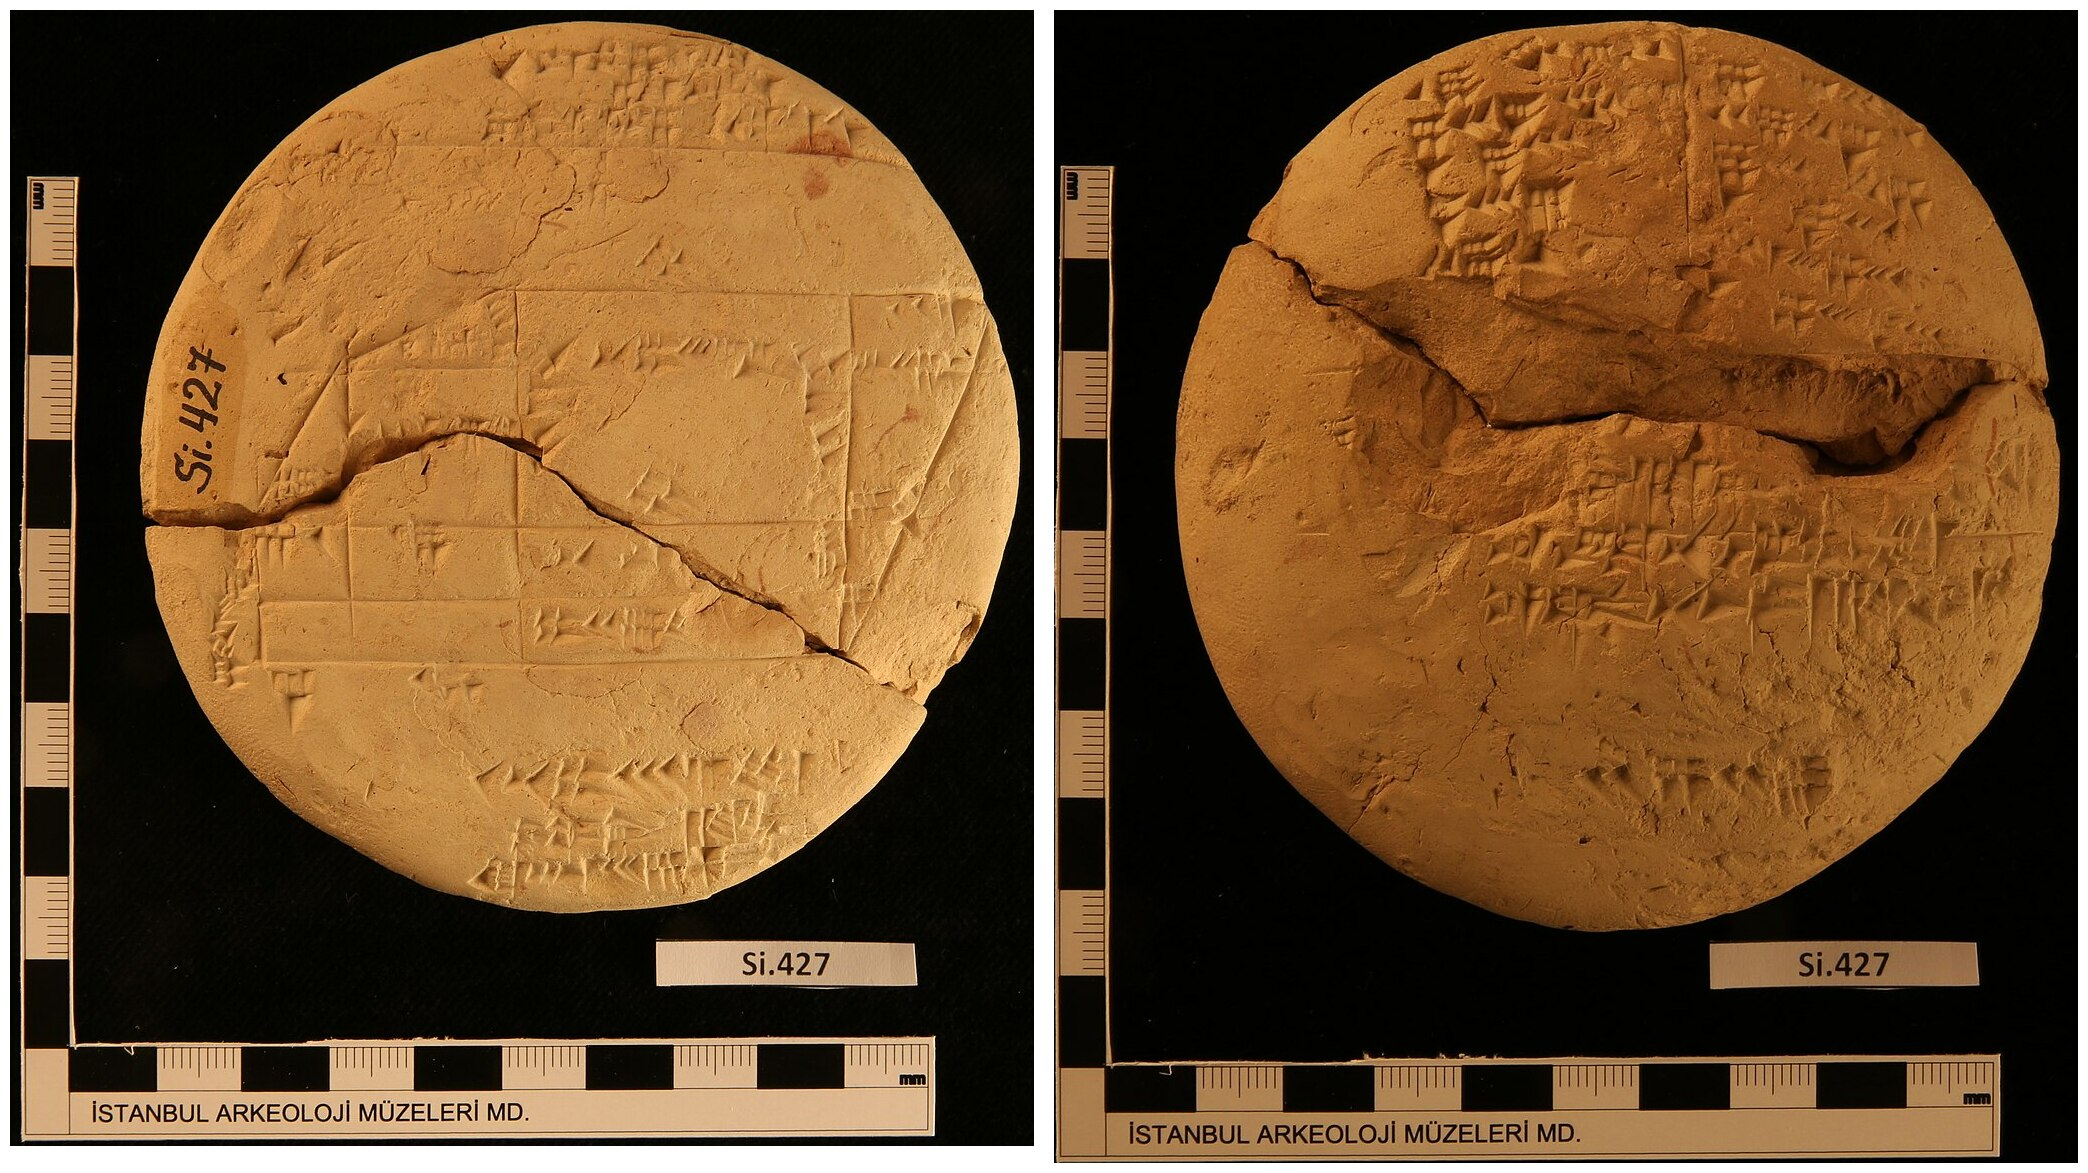
\includegraphics[width=1\linewidth,height=1\textheight]{./figures/si427} 

}

\caption{Photos of the tablet Si. 427 which has recently been identified as the earliest depiction of the Pythagorean theorem [@mansfield2020]. Left: the obverse of the tablet depicts a diagram of a field, inscribed with areas. Right: the reverse of the tablet contains a table of numbers, corresponding to the calculation of the areas. Source: Wikimedia Commons [@mansfield2024].}\label{fig:unnamed-chunk-4}
\end{figure}

For a long time, coordinate systems remained tied to geography and maps. However, with the arrival of the early modern age, this was about to change. In the 16-17th century, the works of the 9th century algebraist Al-Khwarizmi percolated into Europe, and with them the idea of representing unknown quantities by variables (\citeproc{ref-kvasz2006}{Kvasz 2006}). This idea culminated with Descartes, who introduced the concept of visualizing algebraic relationships as objects in a 2D plane, forging a powerful link between Euclidean geometry and algebra (\citeproc{ref-friendly2021}{Friendly and Wainer 2021}). Coordinate systems were thus freed of their connection to geography, and the x- and y-axes could now be used to represent an arbitrary ``space'' spanned by two variables.

Descartes' invention of drawing abstract relationships as objects in a 2D plane was initially only used to plot mathematical functions. However, it would not be long until people realized that observations of the real world could be visualized as well. A true pioneer in this arena was William Playfair, who popularized visualization as a way of presenting socioeconomic data and invented many types of plots still in use today, such as the barplot, lineplot, and pie chart (\citeproc{ref-friendly2021}{Friendly and Wainer 2021}). Further, with the emergence of modern nation states in the 19th century, the collection of data and \emph{statistics} (``things of the state,'' \citeproc{ref-etymonline2024}{Online Etymology Dictionary 2024}) became widespread, leading to a ``golden age'' of statistical graphics (\citeproc{ref-beniger1978}{Beniger and Robyn 1978}; \citeproc{ref-friendly2021}{Friendly and Wainer 2021}; \citeproc{ref-young2011}{Young, Valero-Mora, and Friendly 2011}). This period saw the emergence of other graphical lumnaries, such as Étienne-Jules Marey and Charles Joseph Minard (\citeproc{ref-friendly2021}{Friendly and Wainer 2021}), as well as some ingenious examples of the use of statistical graphics to solve real-world problems, including John Snow's investigation into the London cholera outbreak (\citeproc{ref-freedman1999}{Freedman 1999}; \citeproc{ref-friendly2021}{Friendly and Wainer 2021}) and Florence Nightingale's reporting on the unsanitary treatment of wounded British soldiers during the Crimean War (\citeproc{ref-brasseur2005}{Brasseur 2005}), both of which lead to a great reduction of preventable deaths.

Simultaneously, the field of mathematical statistics was also experiencing significant developments. Building upon the foundation laid by mathematical prodigies such as Jakob Bernoulli, Abraham de Moivre, Pierre Simon Laplace, and Carl Friedrich Gauss, early 19th century pioneers such as Adolph Quetelet and Francis Galton began developing statistical techniques for uncovering hidden trends in the newly unearthed treasure trove of socioeconomic data (\citeproc{ref-fienberg1992}{Fienberg 1992}; \citeproc{ref-freedman1999}{Freedman 1999}). In the late 19th and early 20th century, these initial efforts were greatly advanced by the theoretical work of figures such as Karl Pearson, Ronald A. Fisher, Jerzy Neyman, and Harold Jeffreys, who established statistics as a discipline in its own right and facilitated its dissemination throughout many scientific fields (\citeproc{ref-fienberg1992}{Fienberg 1992}).

As mathematical statistics gained prominence in the early 20th century, data visualization declined. Perceived as less rigorous than ``serious'' statistical analysis, it got relegated to an auxiliary position, ushering in ``dark age'' of statistical graphics (\citeproc{ref-friendly2006}{Friendly 2006}; \citeproc{ref-young2011}{Young, Valero-Mora, and Friendly 2011}). This development may have been partly driven by the early frequentist statisticians' aspiration to establish statistics as a foundation for determining objective truths about the world and society, motivated by personal socio-political goals (see \citeproc{ref-clayton2021}{Clayton 2021}). Be it as it may, while statistical graphics also did get popularized and entered the mainstream during this time, only a few interesting developments took place (\citeproc{ref-friendly2021}{Friendly and Wainer 2021}).

However, beginning in the late 1950's, a series of developments took place which would restore the prominence of data visualization and make it more accessible than ever. Firstly, on the theoretical front, the work of certain academic heavy-weights greatly elevated data visualization and its prestige. Particularly, John Tukey (\citeproc{ref-tukey1962}{1962}; \citeproc{ref-tukey1977}{1977}) fervently championed exploratory data analysis and placed data visualization in its centre. Around the same time, Jacques Bertin published his famous \emph{Sémiologie graphique} (\citeproc{ref-bertin1967}{1967}), which was one of the first works to attempt to lay out a comprehensive system of visual encodings and scales. Secondly, at the more applied level, the development of personal computers (see e.g. \citeproc{ref-abbate1999}{Abbate 1999}) and high-level programming languages such as FORTRAN in 1954 (\citeproc{ref-backus1978}{Backus 1978}), made the process of rendering production-grade figures easier and more accessible than ever before. Combined, these developments fueled a surge in the use and dissemination of data visualizations.

As the millennium drew to a close, several other important developments solidified the foundation of static data visualization. First, William Cleveland made significant contributions to the field, laying out many important principles for scientific data visualization (\citeproc{ref-cleveland1985}{Cleveland 1985}, \citeproc{ref-cleveland1993}{1993}). Of note, his seminal study on the impact of the choice of visual encodings on statistical judgements remains widely cited today (\citeproc{ref-cleveland1984}{Cleveland and McGill 1984}). Similarly, Edward Tufte introduced essential principles for designing effective graphics, coining terms such as \emph{chartjunk} and \emph{data-to-ink ratio} (\citeproc{ref-tufte2001}{Tufte 2001}). Finally, Leland Wilkinson's groundbreaking Grammar of Graphics (\citeproc{ref-wilkinson2012}{2012}) introduced a comprehensive system for designing charts based on simple algebraic rules, influencing nearly every subsequent software package and research endeavor in the field of visualization.

\subsection{Early interactive data visualization: By statisticians for statisticians}\label{early-interactive}

Compared to static data visualization, interactive data visualization is much more of a recent development. Consequently, less has been written about its history, owing to the shorter timeline, as well as the rapid evolution of software in the time since its inception and the proprietary nature of some systems. Nevertheless, the brief history of interactive data visualization is still rather compelling.

Following the boom of static data visualization in the 1950's, interactive data visualization would not be left far behind. It started with tools designed for niche, specialized tasks. For example, Fowlkes (\citeproc{ref-fowlkes1969}{1969}) designed a system which allowed the users to view probability plots under different configurations of parameters and transformations, whereas Kruskal (\citeproc{ref-kruskal1964}{1965}) created a tool for visualizing multidimensional scaling.

\begin{figure}

{\centering 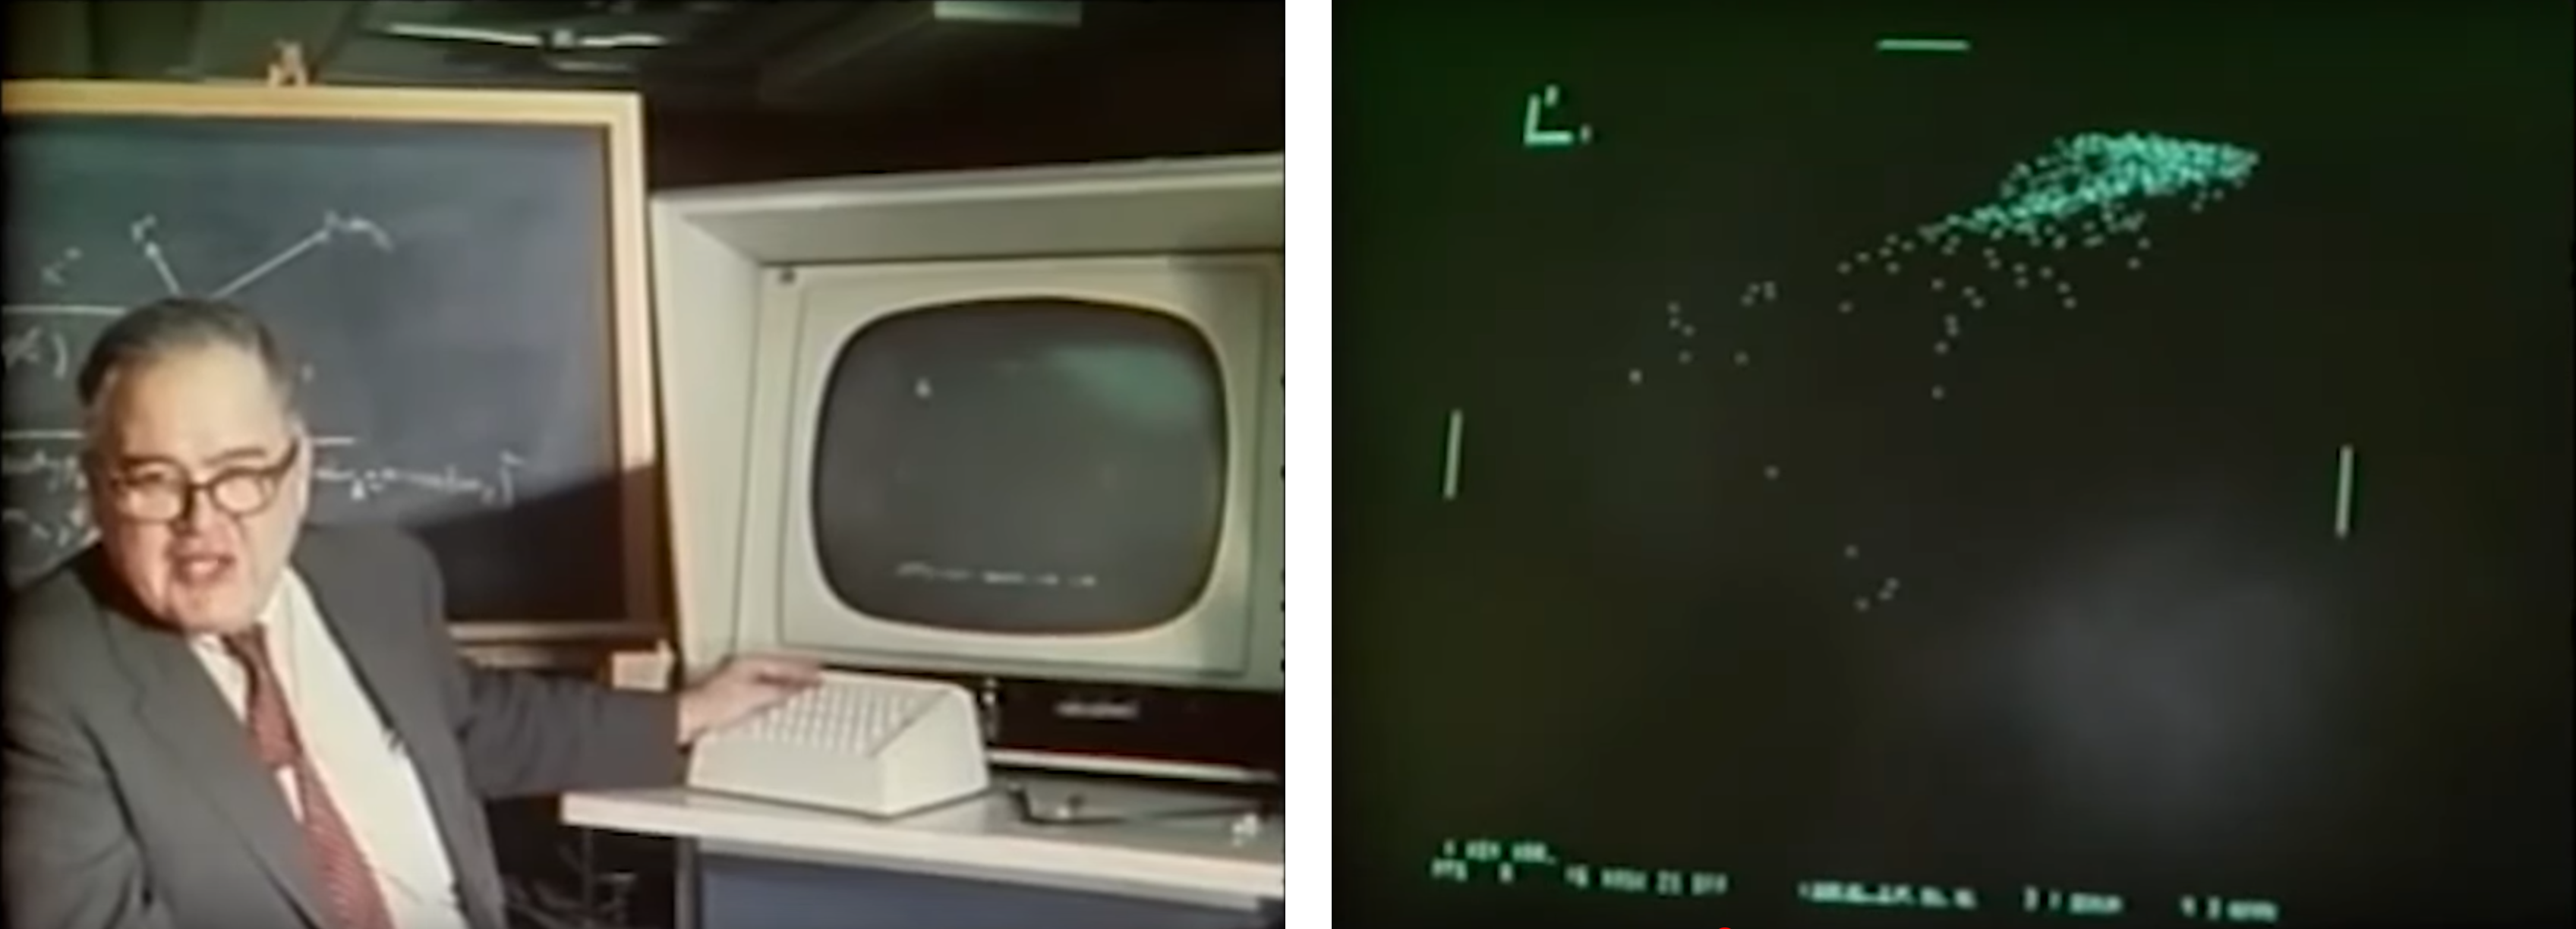
\includegraphics[width=1\linewidth,height=1\textheight]{./figures/prim9} 

}

\caption{John Tukey showcasing the PRIM-9 system (left), with an example of a projected scatterplot [right, @fisherkeller1974]. Screenshots were taken from a video available at: [ASA Statistical Graphics Video Library](https://community.amstat.org/jointscsg-section/media/videos))}\label{fig:unnamed-chunk-5}
\end{figure}

However, researchers soon recognized the potential of interactive data visualization as a general-purpose tool for exploring data. The first such general-purpose system was PRIM-9 (\citeproc{ref-fisherkeller1974}{Fisherkeller, Friedman, and Tukey 1974}). PRIM-9 allowed for exploration of multivariate data via interactive features such as projection, rotation, masking, and filtering. Following PRIM-9, the late 1980's saw the emergence of a new generation of systems which provided an even wider range of capabilities. Tools like MacSpin (\citeproc{ref-donoho1988}{Donoho, Donoho, and Gasko 1988}), Data Desk (\citeproc{ref-velleman1989}{Velleman and Paul 1989}), XLISP-STAT (\citeproc{ref-tierney1990}{L. Tierney 1990}), and XGobi (\citeproc{ref-swayne1998}{Swayne, Cook, and Buja 1998}) introduced features such as interactive scaling, rotation, linked views, and grand tours (for a glimpse into these systems, excellent video-documentaries are available at \href{https://community.amstat.org/jointscsg-section/media/videos}{ASA Statistical Graphics Video Library}).

\begin{figure}

{\centering 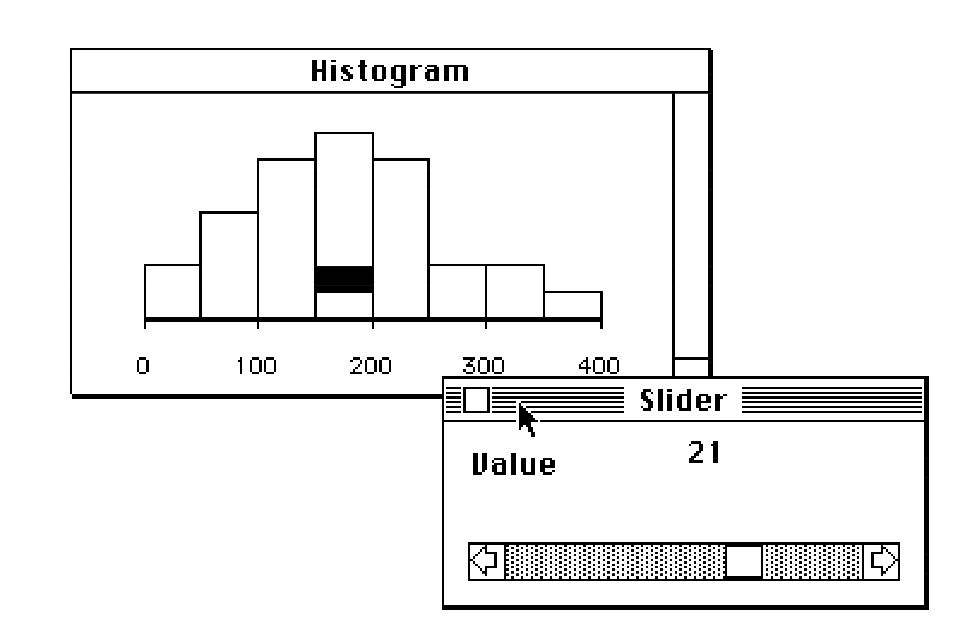
\includegraphics[width=1\linewidth,height=1\textheight]{./figures/xlisp-stat} 

}

\caption{Example of interactive control of histogram highlighting in XLISP-STAT. Note that, unlike in many current data visualization systems, aggregation plots were sensitive to data order (not commutative). This non-commutative behavior meant that, for instance, a highlighted segment could appear in the middle of a bar (as seen in the figure above) or multiple non-adjacent highlighted cases might appear as 'stripes'. Figure reproduced from @tierney1990.}\label{fig:xlisp-stat}
\end{figure}

\subsubsection{Open-source Statistical Computing}\label{open-source-statistical-computing}

The proliferation of open-source, general-purpose statistical computing software such as S and R further democratized the access to interactive data visualization tools (see also \citeproc{ref-leeuw2004}{Leeuw 2004}). Building on XGobi's foundation, GGobi (\citeproc{ref-swayne2003}{Swayne et al. 2003}), expanded upon on XGobi and provided an integration layer for R. Other tools like MANET (\citeproc{ref-unwin1996}{Unwin et al. 1996}) and Mondrian (\citeproc{ref-theus2002}{Theus 2002}) introduced sophisticated linking techniques, with features such as selection sequences, allowing the users to combine a series of selections via logical operators (see also \citeproc{ref-unwin2006}{Unwin et al. 2006}). Further, iPlots (\citeproc{ref-urbanek2003}{Urbanek and Theus 2003}) implemented a general framework for interactive plotting in R, allowing not only for one-shot rendering interactive figures from R but also for direct programmatic manipulation. This package was later expanded expanded for big data capabilities in iPlots eXtreme (\citeproc{ref-urbanek2011}{Urbanek 2011}). Finally, the \texttt{cranvas} package (\citeproc{ref-xie2014}{Xie, Hofmann, and Cheng 2014}) introduced a set of reactive programming primitives that could be used for building the infrastructure underlying interactive graphics directly in R, within the model-view-controller (MVC) framework.

\begin{figure}

{\centering 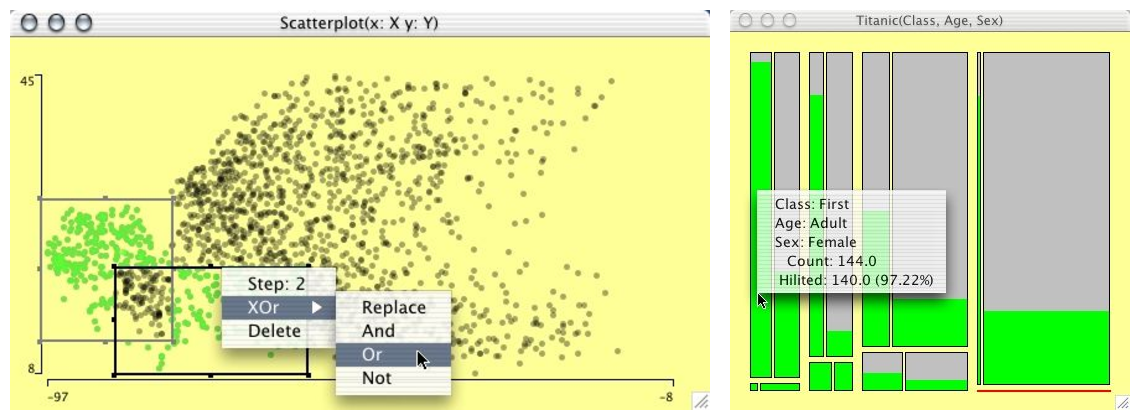
\includegraphics[width=1\linewidth,height=1\textheight]{./figures/mondrian} 

}

\caption{Examples of interactive features in Mondrian [@theus2002]: selection operators (left) and mosaic plot with querying (right).}\label{fig:unnamed-chunk-6}
\end{figure}

Alongside the more general interactive data visualization frameworks mentioned above, there were also more specialized packages designed for specific techniques and models. For instance, \texttt{KLIMT} was developed for interactive visualization of classification and regression trees (\citeproc{ref-urbanek2001}{Urbanek and Unwin 2001}; \citeproc{ref-urbanek2002}{Urbanek 2002}). Similarly, packages like \texttt{tourr} (\citeproc{ref-wickham2011}{Wickham 2011}), \texttt{spinifex} (\citeproc{ref-spyrison2020}{Spyrison and Cook 2020}), \texttt{liminal} (\citeproc{ref-lee2021}{Lee 2021}; \citeproc{ref-lee2022a}{Lee, Laa, and Cook 2022}) provided tools for exploring large multivariate data sets via grand tour projections (see \citeproc{ref-cook1995}{Cook et al. 1995}).

Another important milestone in the history of interactivity in R was the development of Shiny (\citeproc{ref-shiny2024}{W. Chang et al. 2024}; see also \citeproc{ref-sievert2020}{Sievert 2020}; \citeproc{ref-wickham2021}{Wickham 2021}), a general framework for developing web apps in R. Shiny uses a client-server MVC-like model, whereby the user defines an R-based server and a web-based UI/controller layer (which is scaffolded in R, but which transpiles to HTML, CSS, and JavaScript). Bi-directional communication between the client and the server is handled via WebSockets (\citeproc{ref-mdn2024g}{MDN 2025}), facilitated through the \texttt{httpuv} package (\citeproc{ref-cheng2024}{Cheng et al. 2024}). The primary advantage of Shiny is that it gives less technical R users the ability to easily create rich interactive web apps, including interactive data visualizations (by re-rendering static plots). The one major downside of Shiny is that, since every interactive event has to do a round-trip from the client to the R server and back again, high-frequency interactions (such as brushing scatterplot points) can become prohibitively slow, particularly at larger data volumes (although there are ways to mitigate this, \citeproc{ref-sievert2020}{Sievert 2020}).

Over time, there seems to have been a trend towards more of the specialized tools within the R community, and fewer of the general, high-level frameworks (although there were some notable exceptions, such as the \texttt{loon} package, \citeproc{ref-waddell2023}{Waddell and Oldford 2023}). Currently, it seems that R users typically encounter interactive visualizations as part of Shiny (\citeproc{ref-shiny2024}{W. Chang et al. 2024}) dashboards, or through R wrappers of interactive data visualization packages ported over from the JavaScript ecosystem (see Section \ref{web-based}).

\subsubsection{Common features and limitations of early interactive systems}\label{common-features-and-limitations-of-early-interactive-systems}

A common thread among these interactive data visualization systems is that they were designed by statisticians with primary focus on data exploration. High-level analytic features such as linked views, rotation/projection, and interactive manipulation of model parameters made frequent appearance. While these features were powerful, they also contributed to a steeper learning curve, potentially limiting adoption by users without a strong data analytic background. Furthermore, these early tools were typically standalone applications, with only later packages like GGobi and iplots offering integration with other data analysis software and languages. Finally, they often offerered only limited customization options and this made them less suitable for data presentation.

\subsection{Interactive data visualization and the internet: Web-based interactivity}\label{web-based}

The end of the millennium marked the arrival of a new class of technologies which impacted interactive data visualization just as much as almost every other field of human endeavor. The rise of the internet in the mid 1990's made it possible to create interactive applications that could be accessed by anyone, from anywhere. This was aided by the dissemination of robust and standardized web browsers, as well as the development of JavaScript as a high-level programming language for the web (for a tour of the language's history, see e.g. \citeproc{ref-wirfs-brock2020}{Wirfs-Brock and Eich 2020}). Soon, interactive visualizations became just one of many emerging technologies within the burgeoning web ecosystem.

Early web-based interactive data visualization systems tended to rely on external plugins. Examples of these include Prefuse (\citeproc{ref-heer2005}{Heer, Card, and Landay 2005}) and Flare (developed around 2008, \citeproc{ref-flare2020}{Blokt 2020}), which leveraged the Java runtime and Adobe Flash Player, respectively. However, as browser technologies advanced, particularly as JavaScript's performance improved thanks to advances in just-in-time compilation (JIT, see e.g. \citeproc{ref-clark2017}{Clark 2017}; \citeproc{ref-dao2020}{Dao 2020}), it became possible to create complex interactive experiences directly in the browser. This led to the emergence of several popular web-native interactive data visualization systems in the early 2010s, many of which remain widely used today.

\subsubsection{D3}\label{d3}

D3.js (\citeproc{ref-bostock2022}{Mike Bostock 2022}) is one of the earliest and most influential web-based visualization systems. As a general, low-level framework for visualizing data, D3 provides of a suite of specialized JavaScript modules for various aspects of the data visualization workflow, including data parsing, transformation, scaling, and DOM interaction.

For instance, here's how to create a basic scatterplot in D3:

\begin{Shaded}
\begin{Highlighting}[]
\ImportTok{import} \OperatorTok{*} \ImportTok{as}\NormalTok{ d3 }\ImportTok{from} \StringTok{"d3"}\OperatorTok{;}

\KeywordTok{const}\NormalTok{ plot }\OperatorTok{=} \BuiltInTok{document}\OperatorTok{.}\FunctionTok{querySelector}\OperatorTok{\textless{}}\BuiltInTok{HTMLDivElement}\OperatorTok{\textgreater{}}\NormalTok{(}\StringTok{"\#d3{-}plot"}\NormalTok{)}\OperatorTok{!;}
\KeywordTok{const}\NormalTok{ data }\OperatorTok{=}\NormalTok{ [}
\NormalTok{  \{ }\DataTypeTok{x}\OperatorTok{:} \DecValTok{1}\OperatorTok{,} \DataTypeTok{y}\OperatorTok{:} \FloatTok{0.41}\NormalTok{ \}}\OperatorTok{,}
\NormalTok{  \{ }\DataTypeTok{x}\OperatorTok{:} \DecValTok{2}\OperatorTok{,} \DataTypeTok{y}\OperatorTok{:} \FloatTok{4.62}\NormalTok{ \}}\OperatorTok{,}
\NormalTok{  \{ }\DataTypeTok{x}\OperatorTok{:} \DecValTok{3}\OperatorTok{,} \DataTypeTok{y}\OperatorTok{:} \FloatTok{7.62}\NormalTok{ \}}\OperatorTok{,}
\NormalTok{  \{ }\DataTypeTok{x}\OperatorTok{:} \DecValTok{4}\OperatorTok{,} \DataTypeTok{y}\OperatorTok{:} \FloatTok{6.54}\NormalTok{ \}}\OperatorTok{,}
\NormalTok{  \{ }\DataTypeTok{x}\OperatorTok{:} \DecValTok{5}\OperatorTok{,} \DataTypeTok{y}\OperatorTok{:} \FloatTok{9.61}\NormalTok{ \}}\OperatorTok{,}
\NormalTok{]}\OperatorTok{;}

\KeywordTok{const}\NormalTok{ margin }\OperatorTok{=}\NormalTok{ \{ }\DataTypeTok{top}\OperatorTok{:} \DecValTok{10}\OperatorTok{,} \DataTypeTok{right}\OperatorTok{:} \DecValTok{30}\OperatorTok{,} \DataTypeTok{bottom}\OperatorTok{:} \DecValTok{30}\OperatorTok{,} \DataTypeTok{left}\OperatorTok{:} \DecValTok{60}\NormalTok{ \}}\OperatorTok{;}
\KeywordTok{const}\NormalTok{ width }\OperatorTok{=} \PreprocessorTok{parseFloat}\NormalTok{(plot}\OperatorTok{.}\AttributeTok{style}\OperatorTok{.}\AttributeTok{width}\NormalTok{)}\OperatorTok{;}
\KeywordTok{const}\NormalTok{ height }\OperatorTok{=} \PreprocessorTok{parseFloat}\NormalTok{(plot}\OperatorTok{.}\AttributeTok{style}\OperatorTok{.}\AttributeTok{height}\NormalTok{)}\OperatorTok{;}

\CommentTok{// Create a SVG element, resize it, and append it to \#d3{-}plot}
\KeywordTok{const}\NormalTok{ svg }\OperatorTok{=}\NormalTok{ d3}
  \OperatorTok{.}\FunctionTok{select}\NormalTok{(}\StringTok{"\#d3{-}plot"}\NormalTok{)}
  \OperatorTok{.}\FunctionTok{append}\NormalTok{(}\StringTok{"svg"}\NormalTok{)}
  \OperatorTok{.}\FunctionTok{attr}\NormalTok{(}\StringTok{"width"}\OperatorTok{,}\NormalTok{ width }\OperatorTok{+}\NormalTok{ margin}\OperatorTok{.}\AttributeTok{left} \OperatorTok{+}\NormalTok{ margin}\OperatorTok{.}\AttributeTok{right}\NormalTok{)}
  \OperatorTok{.}\FunctionTok{attr}\NormalTok{(}\StringTok{"height"}\OperatorTok{,}\NormalTok{ height }\OperatorTok{+}\NormalTok{ margin}\OperatorTok{.}\AttributeTok{top} \OperatorTok{+}\NormalTok{ margin}\OperatorTok{.}\AttributeTok{bottom}\NormalTok{)}
  \OperatorTok{.}\FunctionTok{append}\NormalTok{(}\StringTok{"g"}\NormalTok{)}
  \OperatorTok{.}\FunctionTok{attr}\NormalTok{(}\StringTok{"transform"}\OperatorTok{,} \StringTok{"translate("} \OperatorTok{+}\NormalTok{ margin}\OperatorTok{.}\AttributeTok{left} \OperatorTok{+} \StringTok{","} \OperatorTok{+}\NormalTok{ margin}\OperatorTok{.}\AttributeTok{top} \OperatorTok{+} \StringTok{")"}\NormalTok{)}\OperatorTok{;}

\CommentTok{// Create x and y scales and append them to}
\KeywordTok{const}\NormalTok{ scaleX }\OperatorTok{=}\NormalTok{ d3}\OperatorTok{.}\FunctionTok{scaleLinear}\NormalTok{()}\OperatorTok{.}\FunctionTok{domain}\NormalTok{([}\DecValTok{0}\OperatorTok{,} \DecValTok{6}\NormalTok{])}\OperatorTok{.}\FunctionTok{range}\NormalTok{([}\DecValTok{0}\OperatorTok{,}\NormalTok{ width])}\OperatorTok{;}
\KeywordTok{const}\NormalTok{ scaleY }\OperatorTok{=}\NormalTok{ d3}\OperatorTok{.}\FunctionTok{scaleLinear}\NormalTok{()}\OperatorTok{.}\FunctionTok{domain}\NormalTok{([}\DecValTok{10}\OperatorTok{,} \DecValTok{0}\NormalTok{])}\OperatorTok{.}\FunctionTok{range}\NormalTok{([}\DecValTok{0}\OperatorTok{,}\NormalTok{ height])}\OperatorTok{;}
\NormalTok{svg}
  \OperatorTok{.}\FunctionTok{append}\NormalTok{(}\StringTok{"g"}\NormalTok{)}
  \OperatorTok{.}\FunctionTok{attr}\NormalTok{(}\StringTok{"transform"}\OperatorTok{,} \StringTok{"translate(0,"} \OperatorTok{+}\NormalTok{ height }\OperatorTok{+} \StringTok{")"}\NormalTok{)}
  \OperatorTok{.}\FunctionTok{call}\NormalTok{(d3}\OperatorTok{.}\FunctionTok{axisBottom}\NormalTok{(scaleX))}\OperatorTok{;}
\NormalTok{svg}\OperatorTok{.}\FunctionTok{append}\NormalTok{(}\StringTok{"g"}\NormalTok{)}\OperatorTok{.}\FunctionTok{call}\NormalTok{(d3}\OperatorTok{.}\FunctionTok{axisLeft}\NormalTok{(scaleY))}\OperatorTok{;}

\CommentTok{// Add points}
\NormalTok{svg}
  \OperatorTok{.}\FunctionTok{append}\NormalTok{(}\StringTok{"g"}\NormalTok{)}
  \OperatorTok{.}\FunctionTok{selectAll}\NormalTok{(}\StringTok{"dot"}\NormalTok{)}
  \OperatorTok{.}\FunctionTok{data}\NormalTok{(data)}
  \OperatorTok{.}\FunctionTok{enter}\NormalTok{()}
  \OperatorTok{.}\FunctionTok{append}\NormalTok{(}\StringTok{"circle"}\NormalTok{)}
  \OperatorTok{.}\FunctionTok{attr}\NormalTok{(}\StringTok{"cx"}\OperatorTok{,}\NormalTok{ (d) }\KeywordTok{=\textgreater{}} \FunctionTok{scaleX}\NormalTok{(d}\OperatorTok{.}\AttributeTok{x}\NormalTok{))}
  \OperatorTok{.}\FunctionTok{attr}\NormalTok{(}\StringTok{"cy"}\OperatorTok{,}\NormalTok{ (d) }\KeywordTok{=\textgreater{}} \FunctionTok{scaleY}\NormalTok{(d}\OperatorTok{.}\AttributeTok{y}\NormalTok{))}
  \OperatorTok{.}\FunctionTok{attr}\NormalTok{(}\StringTok{"r"}\OperatorTok{,} \DecValTok{2}\NormalTok{)}\OperatorTok{;}
\end{Highlighting}
\end{Shaded}

\begin{figure}

{\centering 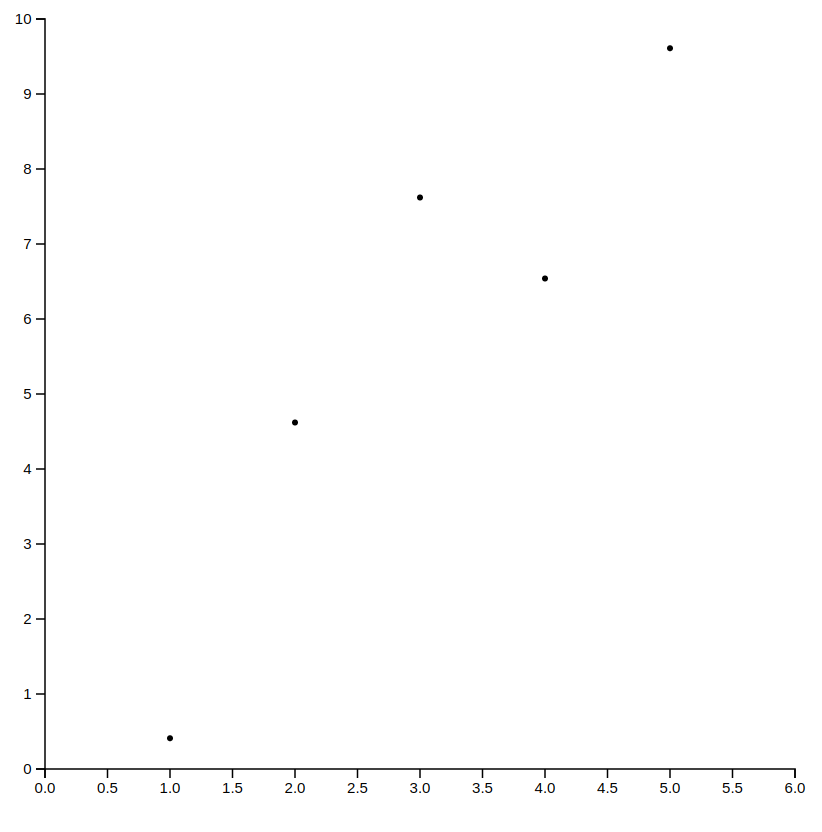
\includegraphics[width=1\linewidth,height=1\textheight]{./figures/d3-scatterplot} 

}

\caption{Example of a scatterplot built with D3.js. The code was taken from D3 Graph Gallery [@holtz2022b] and adjusted to use ES6 syntax and slightly more informative variable names/comments.}\label{fig:d3-scatterplot}
\end{figure}

As you can see from Figure \ref{fig:d3-scatterplot} and the corresponding code, D3 is a fairly low-level framework. Compared to typical high-level plotting functionalities such as those provided by base R or \texttt{ggplot2} (\citeproc{ref-r2024}{R Core Team 2024}; \citeproc{ref-wickham2016}{Wickham 2016}), the user has to handle many low-level details such as scaling and appending of primitives explicitly. This is also the case with interaction. While D3 does provide some methods for handling reactive DOM events, it does not itself provide a system for dispatching and coordinating these events - instead, it delegates this responsibility to the user, and encourages the use of reactive Web frameworks such as React (\citeproc{ref-react2024}{Meta 2024}), Vue (\citeproc{ref-vue2024}{Evan You and the Vue Core Team 2024}), or Svelte (\citeproc{ref-svelte2024}{Rich Harris and the Svelte Core Team 2024}).

Finally, D3.js visualizations are rendered as Scalable Vector Graphics (SVG) by default. This ensures lossless scaling but may impact rendering performance at high data volumes. While various unofficial alternative rendering engines based on the HTML 5 Canvas element or WebGL, do exist, there are no official libraries with such functionalities as of this date.

\subsubsection{Plotly and Highcharts}\label{plotly-and-highcharts}

Building upon the low-level infrastructure that D3 provides, many packages such as Plotly.js (\citeproc{ref-plotly2022}{Plotly Inc. 2022}) and Highcharts (\citeproc{ref-highcharts2024}{Highsoft 2024}) provide high-level abstractions which make the process of building interactive figures easier for the average user. Unlike D3 which provides low-level utilities such as data transformations, scales, and geometric objects, these packages provide a simple declarative framework for rendering entire plots using a static \hyperref[JSON]{JSON} schema.

Here's how we can render the same scatterplot in Plotly, using the R \texttt{plotly} package (\citeproc{ref-sievert2020}{Sievert 2020}):

\begin{Shaded}
\begin{Highlighting}[]
\FunctionTok{library}\NormalTok{(plotly)}
\NormalTok{data }\OtherTok{\textless{}{-}} \FunctionTok{data.frame}\NormalTok{(}\AttributeTok{x =} \DecValTok{1}\SpecialCharTok{:}\DecValTok{5}\NormalTok{, }\AttributeTok{y =} \FunctionTok{c}\NormalTok{(}\FloatTok{0.41}\NormalTok{, }\FloatTok{4.62}\NormalTok{, }\FloatTok{7.62}\NormalTok{, }\FloatTok{6.54}\NormalTok{, }\FloatTok{9.61}\NormalTok{))}
\FunctionTok{plot\_ly}\NormalTok{(data, }\AttributeTok{x =} \SpecialCharTok{\textasciitilde{}}\NormalTok{x, }\AttributeTok{y =} \SpecialCharTok{\textasciitilde{}}\NormalTok{y)}
\end{Highlighting}
\end{Shaded}

\begin{figure}

{\centering 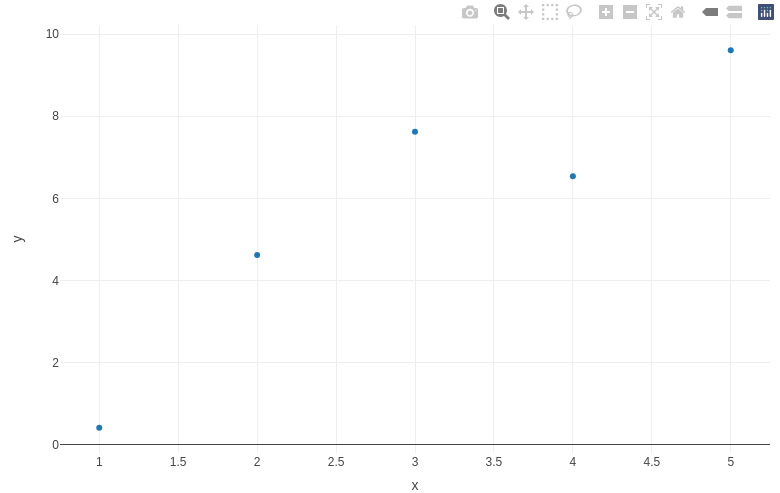
\includegraphics[width=1\linewidth,height=1\textheight]{./figures/plotly-scatterplot} 

}

\caption{Example of a scatterplot with `plotly`.}\label{fig:plotly-scatterplot}
\end{figure}

Here's the correponding code in JavaScript:

\begin{Shaded}
\begin{Highlighting}[]
\KeywordTok{const}\NormalTok{ data }\OperatorTok{=}\NormalTok{ [\{}
  \DataTypeTok{x}\OperatorTok{:}\NormalTok{ [}\DecValTok{1}\OperatorTok{,} \DecValTok{2}\OperatorTok{,} \DecValTok{3}\OperatorTok{,} \DecValTok{4}\OperatorTok{,} \DecValTok{5}\NormalTok{]}\OperatorTok{,}
  \DataTypeTok{y}\OperatorTok{:}\NormalTok{ [}\FloatTok{0.41}\OperatorTok{,} \FloatTok{4.62}\OperatorTok{,} \FloatTok{7.62}\OperatorTok{,} \FloatTok{6.54}\OperatorTok{,} \FloatTok{9.61}\NormalTok{]}\OperatorTok{,}
  \DataTypeTok{mode}\OperatorTok{:} \StringTok{\textquotesingle{}markers\textquotesingle{}}\OperatorTok{,}
  \DataTypeTok{type}\OperatorTok{:} \StringTok{\textquotesingle{}scatter\textquotesingle{}}
\NormalTok{\}]}\OperatorTok{;}

\NormalTok{Plotly}\OperatorTok{.}\FunctionTok{newPlot}\NormalTok{(}\StringTok{\textquotesingle{}app\textquotesingle{}}\OperatorTok{,}\NormalTok{ data)}\OperatorTok{;}
\end{Highlighting}
\end{Shaded}

Clearly, compared to the D3 code used to create Figure \ref{fig:d3-scatterplot}, the code for creating Figure \ref{fig:plotly-scatterplot} is much terser. Many details, such as the axis limits and margins, point size and colour, gridlines, and widgets, are handled implicitly, via default values and automatic inference. Also, note that the figure provides some interactive features by default, such as zooming, panning, and tooltip on hover. Reactivity is handled automatically using systems built on the native DOM Event Target interface (\citeproc{ref-mdn2024a}{MDN 2024a}).

Highcharts provides a similar JSON-based interface for specifying plots. While perhaps slightly more flexible than Plotly, it also requires more verbose specifications. Because of the similarity, I will not provide a separate example here (interested reader should look up the package's website, \citeproc{ref-highcharts2024}{Highsoft 2024}).

Finally, like D3, both plotly.js and Highcharts also render the graphics in SVG by default. However, unlike D3, they both also provide alternative rendering engines based on WebGL (\citeproc{ref-highschartsboost2022}{Highsoft 2022}; \citeproc{ref-plotly2024b}{Plotly Inc. 2024}). This makes them more ergonomic for use with large data sets.

\subsubsection{Vega and Vega-Lite}\label{vega-and-vega-lite}

Vega (\citeproc{ref-satyanarayan2015}{Satyanarayan et al. 2015}; \citeproc{ref-vega2024a}{Vega Project 2024d}) is another popular interactive data visualization package. Like Plotly and Highcharts, Vega is also partially built upon the foundation of D3 and uses JSON schema for plot specification. However, Vega is more low-level and implements a lot of custom functionality. This allows it to offer more fine-grained customization of graphics and interactive behavior, leading to greater flexibility.

However, this added flexibility does come at a cost. Compared to the high-level frameworks like Plotly and Highcharts, Vega is significantly more verbose. For instance, creating a scatterplot matrix with linked selection in Vega requires over 300 lines of JSON specification, not including the data and using default formatting (\citeproc{ref-vega2024b}{Vega Project 2024b}).

Vega-Lite (\citeproc{ref-satyanarayan2015}{Satyanarayan et al. 2015}) attempts to remedy this complexity by providing a high-level interface to Vega. Here's how we can define a scatterplot with zooming, panning, and tooltip on hover in Vega-Lite:

\begin{Shaded}
\begin{Highlighting}[]
\FunctionTok{library}\NormalTok{(vegawidget)}

\NormalTok{plot\_spec }\OtherTok{\textless{}{-}} \FunctionTok{list}\NormalTok{(}
    \StringTok{\textasciigrave{}}\AttributeTok{$schema}\StringTok{\textasciigrave{}} \OtherTok{=} \FunctionTok{vega\_schema}\NormalTok{(),}
    \AttributeTok{width =} \DecValTok{500}\NormalTok{,}
    \AttributeTok{height =} \DecValTok{300}\NormalTok{,}
    \AttributeTok{data =} \FunctionTok{list}\NormalTok{(}\AttributeTok{values =}\NormalTok{ data),}
    \AttributeTok{mark =} \FunctionTok{list}\NormalTok{(}\AttributeTok{type =} \StringTok{"point"}\NormalTok{, }\AttributeTok{tooltip =} \ConstantTok{TRUE}\NormalTok{),}
    \AttributeTok{encoding =} \FunctionTok{list}\NormalTok{(}
      \AttributeTok{x =} \FunctionTok{list}\NormalTok{(}\AttributeTok{field =} \StringTok{"x"}\NormalTok{, }\AttributeTok{type =} \StringTok{"quantitative"}\NormalTok{),}
      \AttributeTok{y =} \FunctionTok{list}\NormalTok{(}\AttributeTok{field =} \StringTok{"y"}\NormalTok{, }\AttributeTok{type =} \StringTok{"quantitative"}\NormalTok{)}
\NormalTok{    ),}
    \AttributeTok{params =} \FunctionTok{list}\NormalTok{(}\FunctionTok{list}\NormalTok{(}\AttributeTok{name =} \StringTok{"grid"}\NormalTok{, }
                       \AttributeTok{select =} \StringTok{"interval"}\NormalTok{, }
                       \AttributeTok{bind =} \StringTok{"scales"}\NormalTok{))}
\NormalTok{  )}

\NormalTok{plot\_spec }\SpecialCharTok{|\textgreater{}} \FunctionTok{vegawidget}\NormalTok{()}
\end{Highlighting}
\end{Shaded}

\begin{figure}

{\centering 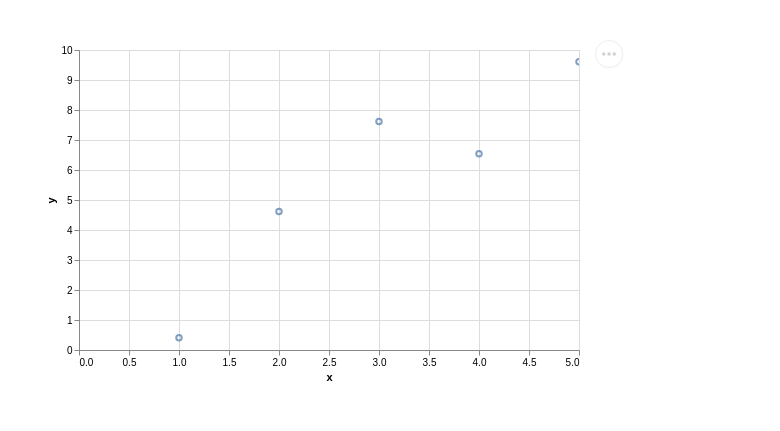
\includegraphics[width=1\linewidth,height=1\textheight]{./figures/vegalite-scatterplot} 

}

\caption{Example of a scatterplot built with `vegalite`.}\label{fig:vegalite-scatterplot}
\end{figure}

Just for clarity, the R code above corresponds to the following declarative JSON schema:

\begin{Shaded}
\begin{Highlighting}[]
\NormalTok{\{}
  \DataTypeTok{$schema}\OperatorTok{:} \StringTok{"https://vega.github.io/schema/vega{-}lite/v5.json"}\OperatorTok{,}
  \DataTypeTok{width}\OperatorTok{:} \DecValTok{500}\OperatorTok{,}
  \DataTypeTok{height}\OperatorTok{:} \DecValTok{300}\OperatorTok{,}
  \DataTypeTok{data}\OperatorTok{:}\NormalTok{ \{ }\DataTypeTok{values}\OperatorTok{:}\NormalTok{ [}
\NormalTok{    \{ }\DataTypeTok{x}\OperatorTok{:} \DecValTok{1}\OperatorTok{,} \DataTypeTok{y}\OperatorTok{:} \FloatTok{0.41}\NormalTok{ \}}\OperatorTok{,}
\NormalTok{    \{ }\DataTypeTok{x}\OperatorTok{:} \DecValTok{2}\OperatorTok{,} \DataTypeTok{y}\OperatorTok{:} \FloatTok{4.62}\NormalTok{ \}}\OperatorTok{,}
\NormalTok{    \{ }\DataTypeTok{x}\OperatorTok{:} \DecValTok{3}\OperatorTok{,} \DataTypeTok{y}\OperatorTok{:} \FloatTok{7.62}\NormalTok{ \}}\OperatorTok{,}
\NormalTok{    \{ }\DataTypeTok{x}\OperatorTok{:} \DecValTok{4}\OperatorTok{,} \DataTypeTok{y}\OperatorTok{:} \FloatTok{6.54}\NormalTok{ \}}\OperatorTok{,}
\NormalTok{    \{ }\DataTypeTok{x}\OperatorTok{:} \DecValTok{5}\OperatorTok{,} \DataTypeTok{y}\OperatorTok{:} \FloatTok{9.61}\NormalTok{ \}]}
\NormalTok{  \}}\OperatorTok{,}
  \DataTypeTok{mark}\OperatorTok{:}\NormalTok{ \{}\StringTok{"type"}\OperatorTok{:} \StringTok{"point"}\OperatorTok{,} \StringTok{"tooltip"}\OperatorTok{:} \KeywordTok{true}\NormalTok{\}}\OperatorTok{,}
  \DataTypeTok{encoding}\OperatorTok{:}\NormalTok{ \{}
    \DataTypeTok{x}\OperatorTok{:}\NormalTok{ \{ }\DataTypeTok{field}\OperatorTok{:} \StringTok{"x"}\OperatorTok{,} \DataTypeTok{type}\OperatorTok{:} \StringTok{"quantitative"}\NormalTok{ \}}\OperatorTok{,}
    \DataTypeTok{y}\OperatorTok{:}\NormalTok{ \{ }\DataTypeTok{field}\OperatorTok{:} \StringTok{"y"}\OperatorTok{,} \DataTypeTok{type}\OperatorTok{:} \StringTok{"quantitative"}\NormalTok{ \}}
\NormalTok{  \}}\OperatorTok{,}
  \DataTypeTok{params}\OperatorTok{:}\NormalTok{ [\{ }\DataTypeTok{name}\OperatorTok{:} \StringTok{"grid"}\OperatorTok{,} \DataTypeTok{select}\OperatorTok{:} \StringTok{"interval"}\OperatorTok{,} \DataTypeTok{bind}\OperatorTok{:} \StringTok{"scales"}\NormalTok{ \}]}
\NormalTok{\}}\OperatorTok{;}
\end{Highlighting}
\end{Shaded}

Note that the zooming and panning capability is provided by the \texttt{params} property, which declaratively specifies a list of plot parameters that can be modified by interaction (see \citeproc{ref-vegalite2024a}{Vega Project 2024c}). In the case above, the specification creates a two-way binding between plot scales and mouse selection events (\citeproc{ref-vegalite2024b}{Vega Project 2024a}).

\subsubsection{Common features and limitations of web-based interactive systems}\label{common-features-and-limitations-of-web-based-interactive-systems}

In general, these contemporary web-based interactive data visualization systems offer a great deal of flexibility, making them well-suited to modern data presentation. However, all of this expressiveness does seem to come at a cost. Compared to the earlier statistical graphics systems, described in Section \ref{early-interactive}, many of the more advanced features that used to be common are either missing or require a significant effort to implement, such that they are only accessible to expert users. This is evidenced by their infrequent appearance in documentation and example gallery pages.

For instance, the \href{https://r-graph-gallery.com/interactive-charts.html}{R Graph Gallery entry on Interactive Charts} (\citeproc{ref-holtz2022}{Holtz 2022}) features multiple interactive figures implemented in the JavaScript libraries described above. However, all of these examples show only surface-level, single-plot interactive features such zooming, panning, hovering, 3D rotation, and node repositioning. The \href{https://dash.plotly.com/interactive-graphing}{Plotly Dash documentation page on Interactive Visualizations} (\citeproc{ref-plotly2022}{Plotly Inc. 2022}) does feature two examples of simple linked cross-filtering, however, the vast majority of visualizations in the \href{https://plotly.com/r/}{Plotly R Open Source Graphing Library documentation page} (\citeproc{ref-plotly2022}{Plotly Inc. 2022}) show examples only surface-level interactivity. Similarly, \href{https://vega.github.io/vega-lite/examples/\#interactive-charts}{VegaLite Gallery pages on Interactive Charts} (\citeproc{ref-vegalite2022}{Vega Project 2022}) feature many examples, however, only a limited number of examples show linked or parametric interactivity (see e.g.~\href{https://vega.github.io/vega-lite/examples/\#interactive-multi-view-displays}{Interactive Multiview Displays}). Finally, the \href{https://jkunst.com/highcharter/articles/showcase.html}{Highcharter Showcase Page} (\citeproc{ref-kunst2022}{Kunst 2022}) does not feature any examples of linking.

Even when advanced features such as linking and parametric manipulation are supported, they are often limited in some way. For example, the following is a quote from the website of Crosstalk, a package designed to enable linking in R, using web-based interactive widgets created with the \texttt{htmlwidgets} package (\citeproc{ref-htmlwidgets2021}{Vaidyanathan et al. 2021}) or R Shiny (\citeproc{ref-shiny2024}{W. Chang et al. 2024}):

\begin{quote}
``Crosstalk currently only works for linked brushing and filtering of views that show individual data points, not aggregate or summary views (where ``observations'' is defined as a single row in a data frame). For example, histograms are not supported since each bar represents multiple data points; but scatter plot points each represent a single data point, so they are supported.''

\begin{itemize}
\tightlist
\item
  Posit (formerly RStudio Inc.) (\citeproc{ref-crosstalk2025}{2025})
\end{itemize}
\end{quote}

Of course, with enough effort, these web-based visualization systems can still be used to create rich figures with advanced interactive features such as linked views and parametric interaction. However, implementing these features often requires stepping down a level of abstraction and dealing with low-level language primitives. This defeats the purpose of using a high-level libraries and creates a barrier to entry for casual users (\citeproc{ref-keller2024}{Keller, Manz, and Gehlenborg 2024}). It also may explain why interactive visualizations are nowadays mainly used for data presentation, not data exploration (\citeproc{ref-batch2017}{Batch and Elmqvist 2017}). With the high upfront cost of learning these package's APIs, creating rich interactive figures may be a task best suited for dedicated developers working inside large organizations, rather than individual researchers/analysts.

\section{What even is interactive data visualization?}\label{what-is-interactive-visualization}

\begin{quote}
If it looks like a duck, swims like a duck, and quacks like a duck, then it probably is a duck.

{[}\ldots{]} The irony is that while the phrase is often cited as proof of abductive reasoning, it is not proof, as the mechanical duck is still not a living duck

\href{https://en.wikipedia.org/wiki/Duck_test}{Duck Test} entry, (\citeproc{ref-wikipedia2022}{Wikipedia 2022})
\end{quote}

In the previous section (Section \ref{brief-history}), I provided an overview of the history and present state of interactive data visualization, discussing a number of features and systems. However, while doing so, I avoided one crucial question: what constitutes an interactive data visualization?

Surprisingly, despite the widespread popularity of interactive visualizations, there is no universally agreed-upon definition of interactivity (\citeproc{ref-vanderplas2020}{Vanderplas, Cook, and Hofmann 2020}). Within the data visualization literature, the terms ``interactive'' and ``interaction'' are rarely explicitly defined. And even when they are, the definitions are often incongruent or even contradictory (see e.g. \citeproc{ref-dimara2019}{Dimara and Perin 2019}; \citeproc{ref-elmqvist2011}{Elmqvist et al. 2011}; \citeproc{ref-pike2009}{Pike et al. 2009}). Finally, similar conceptual ambiguity extends to other terms commonly used in the field, such as a ``dashboard'' (\citeproc{ref-sarikaya2018}{Sarikaya et al. 2018}).

This lack of a clear consensus makes the task of discussing interactive data visualization difficult. Ignoring the issue could lead to confusion, while a truly comprehensive dive into the terminology surrounding interactive data visualization could become excessively verbose, as evidenced by the existence of research papers dedicated to the topic (see e.g. \citeproc{ref-dimara2019}{Dimara and Perin 2019}; \citeproc{ref-elmqvist2011}{Elmqvist et al. 2011}). To address this issue, this section aims to provide a concise overview of how interactivity has been conceptualized in the literature. The goal is to establish a clear framework for understanding ``interactive'' and ``interaction'' within the context of this thesis.

\subsection{Interactive vs.~interacting with}\label{interactive-interacting}

First, the word ``visualization'' in ``interactive data visualization'' can be interpreted in two different ways:

\begin{enumerate}
\def\labelenumi{\arabic{enumi}.}
\tightlist
\item
  As a noun: a concrete chart or figure
\item
  As a nominalized verb: the process of interacting with a figure
\end{enumerate}

In data visualization literature, both interpretations are frequently used, leading to significant ambiguity (\citeproc{ref-dimara2019}{Dimara and Perin 2019}; \citeproc{ref-pike2009}{Pike et al. 2009}; see also \citeproc{ref-yi2007}{Yi et al. 2007}). On one hand, some researchers focus on the mathematical and computational aspects of visualization, discussing specific systems and implementations (see e.g. \citeproc{ref-buja1996}{Buja, Cook, and Swayne 1996}; \citeproc{ref-kelleher2015}{Kelleher and Levkowitz 2015}; \citeproc{ref-leman2013}{Leman et al. 2013}; \citeproc{ref-wills2008}{G. Wills 2008}). Others prioritize the more cognitive or human-computer interaction (HCI) aspects of interactive data visualization, exploring what impact different kinds of visualization techniques have on the user's ability to derive insights from the data (see e.g. \citeproc{ref-brehmer2013}{Brehmer and Munzner 2013}; \citeproc{ref-dimara2019}{Dimara and Perin 2019}; \citeproc{ref-dix1998}{Dix and Ellis 1998}; \citeproc{ref-pike2009}{Pike et al. 2009}; \citeproc{ref-quadri2021}{Quadri and Rosen 2021}; \citeproc{ref-yi2007}{Yi et al. 2007}).

Of course, many interactive data visualization papers discuss both implementation and user experience. However, the dual interpretation of the term ``interactive data visualization'' does complicate literature search. It also highlights the interdisciplinary nature of the field, showing its connections to statistics, computer science, applied mathematics, business analytics, HCI, and cognitive psychology (see \citeproc{ref-brehmer2013}{Brehmer and Munzner 2013}; \citeproc{ref-dimara2019}{Dimara and Perin 2019}). While this interdisciplinary nature of interactive data visualization is certainly a strength, it can also lead to confusion. As such I think it is necessary to clearly define key terms.

To ensure clarity throughout thesis, the term \emph{``interactive data visualization''} will primarily refer to concrete charts or figures. When referring to the \emph{practice} of interactive data visualization, I will attempt to use more active phrasing such as \emph{``interacting with a visualization''} or \emph{``user's interaction with a visualization''}, to indicate that what is being referred to is the activity or process of visualization, rather than any concrete figure or chart.

\subsection{\texorpdfstring{Interactive \emph{enough}?}{Interactive enough?}}\label{interactive-enough}

Even when we use the term ``interactive data visualization'' to refer to concrete charts or figures, the meaning still remains fairly ambiguous. What is the bar for calling a figure ``interactive''? What features should interactive figures have? Surprisingly, it is hard to find consensus on these topics among data visualization researchers, and the criteria tend to vary a lot, such that the same figure may be considered interactive by some but not by others.

Some researchers adopt a broad definition of interactive data visualization, considering almost any figure combined with an interactive graphical user interface (GUI) as interactive, as long as it allows for some level of user manipulation (\citeproc{ref-brodbeck2009}{Brodbeck, Mazza, and Lalanne 2009}). For others, the speed of the computer's responses to user input is important, with faster updates translating to greater interactivity (\citeproc{ref-becker1987}{Becker and Cleveland 1987}; \citeproc{ref-buja1996}{Buja, Cook, and Swayne 1996}). Some also differentiate between ``interactive'' and ``dynamic'' manipulation, such that interactive manipulation involves discrete actions such as pressing a button or selecting an item from a drop-down menu, whereas dynamic manipulation involves continuous actions, like moving a slider or clicking-and-dragging to highlight a rectangular area (\citeproc{ref-rheingans2002}{Rheingans 2002}; \citeproc{ref-jankun2007}{Jankun-Kelly, Ma, and Gertz 2007}; see also \citeproc{ref-dimara2019}{Dimara and Perin 2019}).

However, many other researchers ascribe to a much narrower view of interactive data visualization, which hinges on high-level analytic features that allow efficient exploration of the data. These features include the ability to generate different views of the data (by e.g.~zooming, panning, sorting, and filtering), and the reactive propagation of changes between connected or ``linked'' parts of a figure (\citeproc{ref-kehrer2012}{Kehrer et al. 2012}; \citeproc{ref-buja1996}{Buja, Cook, and Swayne 1996}; \citeproc{ref-keim2002}{Keim 2002}; \citeproc{ref-unwin1999}{Unwin 1999}; \citeproc{ref-chen2008}{Chen et al. 2008}). An often cited guideline is the visual information seeking mantra: overview first, zoom and filter, then details-on-demand (\citeproc{ref-shneiderman2003}{Shneiderman 2003}). Similarly, in visual analytics research, a distinction is made between ``surface-level'' (or ``low-level'') and ``parametric'' (or ``high-level'') interactions, where surface-level interactions manipulate attributes of the visual domain only (e.g.~zooming and panning), whereas parametric interactions manipulate attributes of mathematical models or algorithms underlying the visualization (\citeproc{ref-leman2013}{Leman et al. 2013}; \citeproc{ref-self2018}{Self et al. 2018}; \citeproc{ref-pike2009}{Pike et al. 2009}).

Table \ref{tab:definitions} provides a concise summary of the several perspectives on interactivity discussed above. It meant to serve as a reference point for future discussions within the text, though it is important to note that this is not an exhaustive list. For a more comprehensive taxonomy of interactive visualization systems and features, see e.g. Dimara and Perin (\citeproc{ref-dimara2019}{2019}), Yi et al. (\citeproc{ref-yi2007}{2007}).

\begin{table}
\centering
\caption{\label{tab:definitions}Summary of the perspectives on interactivity}
\centering
\begin{tabular}[t]{l|l|l}
\hline
Name & Details & Selected references\\
\hline
User interaction & The user can interactively manipulate the figure in some way & @brodbeck2009\\
\hline
Real-time updates & The user's interactions propagate into the visualization with little to no lag & @becker1987, @buja1996, @jankun2007, and @rheingans2002\\
\hline
Plot- and data-space manipulation & The user can interactively explore different parts of the data set by doing actions which effectively amount to "subsetting" rows of the data (e.g. zooming, panning, and filtering) & @buja1996, @keim2002, @shneiderman2003, and @unwin1999\\
\hline
Linked views & The user's interactions propagate across multiple plots (e.g. linked highlighting) & @buja1996, @keim2002, @kehrer2012, @unwin1999, @theus2008, @wilhelm2008, @wills2008\\
\hline
Parametric updates & The user can manipulate the parameters of some underlying mathematical model or algorithm (e.g. histogram bins, grand tour projections, etc...) & @leman2013, @pike2009\\
\hline
\end{tabular}
\end{table}

\subsection{Complexity of interactive features}\label{complexity-of-features}

The way we define interactivity is not just a matter of taste or preference: it has a significant impact on the complexity and feasibility of our systems. As we will see in Section \ref{common-features}, some simple features are fairly easy to implement, requiring just a thin interactive layer over a static data visualization system, whereas others come with a significant overhead, requiring an entirely different framework than static visualization.

To make the point with a particularly blunt example, many programming languages support a read-evaluate-print loop (REPL). This allows interactive code execution from the command line: the user inputs code, the interpreter evaluates it, outputs results, and waits for more input. If the language supports plotting, running code to generate plots could be considered an ``interactive data visualization system.'' User interaction with the REPL modifies the visual output, and with fast-enough input, updates could appear almost instantly (thus satisfying the user interaction and real-time update definitions of interactivity, see table). This would make almost every programming language an ``interactive data visualization system'', requiring no additional effort.

However, I would argue that, today, this view stretches the concept of interactivity. It is true that, historically, the command line was considered a highly interactive user interface (see e.g. \citeproc{ref-foley1990}{Foley 1990}; \citeproc{ref-howard1995}{Howard and MacEachren 1995}). However, with advancements in processor speeds and the widespread adoption of graphical user interfaces (GUIs), user expectations have evolved. Nowadays, we typically associate interactivity with direct manipulation of visual elements and immediate feedback (\citeproc{ref-dimara2019}{Dimara and Perin 2019}; \citeproc{ref-urbanek2011}{Urbanek 2011}). Thus, we can see that what's considered ``interactive'' evolves over time.

But even with figures that are manipulated directly, there still are considerable differences in what different features imply for implementation requirements. Some features, like changing color or opacity of points in a scatterplot affect only the visual attributes of the plot and not the underlying data representation. This makes them simple to implement as they do not require any specialized data structures or complex computations, and the primary cost lies in re-rendering the visualization.

In contrast, some interactive features require a lot more infrastructure. For instance, filtering, linked highlighting, or parametric interaction require specialized data structures and algorithms beyond those that would be required in static plots. This is because, each time the user engages in an interaction, entirely new summaries of the underlying data may need to be computed.

To give a concrete example, when a user selects several points in a linked scatterplot (see Section \ref{linked-selection}), we first have to find the ids of all the selected cases, recompute the statistics underlying all other linked plots (such as counts/sums in barplots or histograms), train all of the relevant scales, and only then can we re-render the figure. Likewise, when interactively manipulating a histogram's binwidth, we need to recompute the number of cases in each bin whenever the binwidth changes. To maintain the illusion of smooth, ``continuous'' interaction (\citeproc{ref-dimara2019}{Dimara and Perin 2019}), these computations need to happen fast, and as such, computational efficiency becomes imperative at high data volumes.

\subsection{Working definition}\label{working-definition}

As discussed in previous sections, the definition ``interactive data visualization'' varies across fields and researchers. Moreover, when building interactive data visualization systems, different definitions imply varying levels of implementation complexity. Thus, we need to establish clear criteria for our specific definition.

Data visualization can be broadly categorized into two primary modes: presentation and exploration. While both modes share a bulk of common techniques, each comes with a different set of goals and challenges (\citeproc{ref-kosara2016}{Kosara 2016}). Data presentation starts from the assumption that we have derived most of the important insights from our data already, and the goal is now to communicate these insights clearly and make an impactful and lasting impression (\citeproc{ref-kosara2016}{Kosara 2016}). In contrast, data exploration begins from a position of incomplete knowledge - we accept that there are facts about our data we might not be aware of. Thus, when we explore data with visualizations, the goal is to help us see what we might otherwise miss or might not even think to look for (\citeproc{ref-tukey1977}{Tukey et al. 1977}; \citeproc{ref-unwin2018}{Unwin 2018}).

However, it is not always the case that more complex visuals necessarily translate to better statistical insights. In static visualization, it is a well-established that plots can include seemingly sophisticated features which do not promote the acquisition of statistical insights in any way (\citeproc{ref-cairo2014}{Cairo 2014}, \citeproc{ref-cairo2019}{2019}; \citeproc{ref-gelman2013}{Gelman and Unwin 2013}; \citeproc{ref-tufte2001}{Tufte 2001}). Similarly, adding interactivity to a visualization does not always improve its statistical legibility (see e.g. \citeproc{ref-abukhodair2013}{Abukhodair et al. 2013}; \citeproc{ref-franconeri2021}{Franconeri et al. 2021}).

I propose to treat interactive features the same way we treat visual features in static visualization. Specifically, I propose the following working definition:

\begin{quote}
When building interactive data visualization systems, we should prioritize interactive features which promote statistical understanding.
\end{quote}

If we accept this proposition, then several important consequences follow. First, we must favor high-level, data-dependent, parametric interactions over the purely graphical ones. That is not to say that purely graphical interactive features cannot useful. For instance, in the case of overplotting, changing the size or alpha of points in a scatterplot can help us see features that would otherwise remain hidden. Nevertheless, I argue that the ability to see entirely new representations of the data is what makes some interactive data visualizations systems particularly powerful. The interactive features that enable this, such as linked highlighting and parameter manipulation, go beyond aesthetics, and empower the users to explore the data in a much more dynamic way, compared to static graphics.

\subsection{Common interactive features}\label{common-features}

This section describes several common types of interactive features that tend to frequently appear in general interactive data visualization systems. It is only meant as an overview (for more comprehensive taxonomies of interactive features, see \citeproc{ref-dimara2019}{Dimara and Perin 2019}; \citeproc{ref-unwin2006}{Unwin et al. 2006}; \citeproc{ref-yi2007}{Yi et al. 2007}). For each feature, I highlight its core properties, common use cases, and implementation requirements.

\subsubsection{Changing size and opacity}\label{changing-size-and-opacity}

One of the simplest and most widely-implemented interactive features is the ability to adjust the size and opacity of geometric objects. This feature gives the user the ability to dynamically shrink or grow objects and make semi-transparent, fully transparent, or opaque.

The ability to shrink objects or make them semi-transparent can be particularly useful at high data volumes, since this can reveal trends that may be otherwise hidden due to overplotting. For example, in scatterplots, shrinking points and making them semi-transparent makes it possible to identify high-density regions and can in fact provide an approximation to a 2D kernel density plot (see e.g. \citeproc{ref-dang2010}{Dang, Wilkinson, and Anand 2010}). The same applies to all other types of plots where the where objects or glyphs may be plotted on top of each other at high densities, such as parallel coordinate plots (\citeproc{ref-theus2008}{Theus 2008}).

This feature usually fairly easy to implement, since it involves manipulating visual attributes only. Specifically, in many interactive systems, size and alpha multipliers are independent parameters of the visual representation, which do not depend on the underlying data in any way. In other words, when we manipulate size or opacity of geometric objects in our plots, we do not need to worry about what data these objects represent. Compared to other interactive features, this makes it relatively simple to add this functionality to an existing static visualization system (see \citeproc{ref-bracsoveanu2017}{Braşoveanu et al. 2017}).

\subsubsection{Zooming and panning}\label{zooming-and-panning}

Another two significantly related interactive features are zooming and panning. They are often used in tandem, and both involve interactive manipulation of scale limits. For this reason, I discuss them here simultaneously, in a single subsection.

Zooming, depicted in Figure \ref{fig:zooming}, allows the user to magnify into a specific region of a plot. A common approach involves creating a rectangular selection and the axis scales are then automatically adjusted to match this region, however, other techniques do exist, for instance a symmetric zoom centered on a point using a mouse wheel. Zooming is useful because it allows the user to get a better sense of the trend within the magnified region, and discover patterns that may be otherwise obscured due to overplotting or improper aspect ratio (see e.g. \citeproc{ref-buja1996}{Buja, Cook, and Swayne 1996}; \citeproc{ref-dix1998}{Dix and Ellis 1998}; \citeproc{ref-unwin1999}{Unwin 1999}; \citeproc{ref-theus2008}{Theus 2008}; \citeproc{ref-yi2007}{Yi et al. 2007}).

\begin{figure}

{\centering 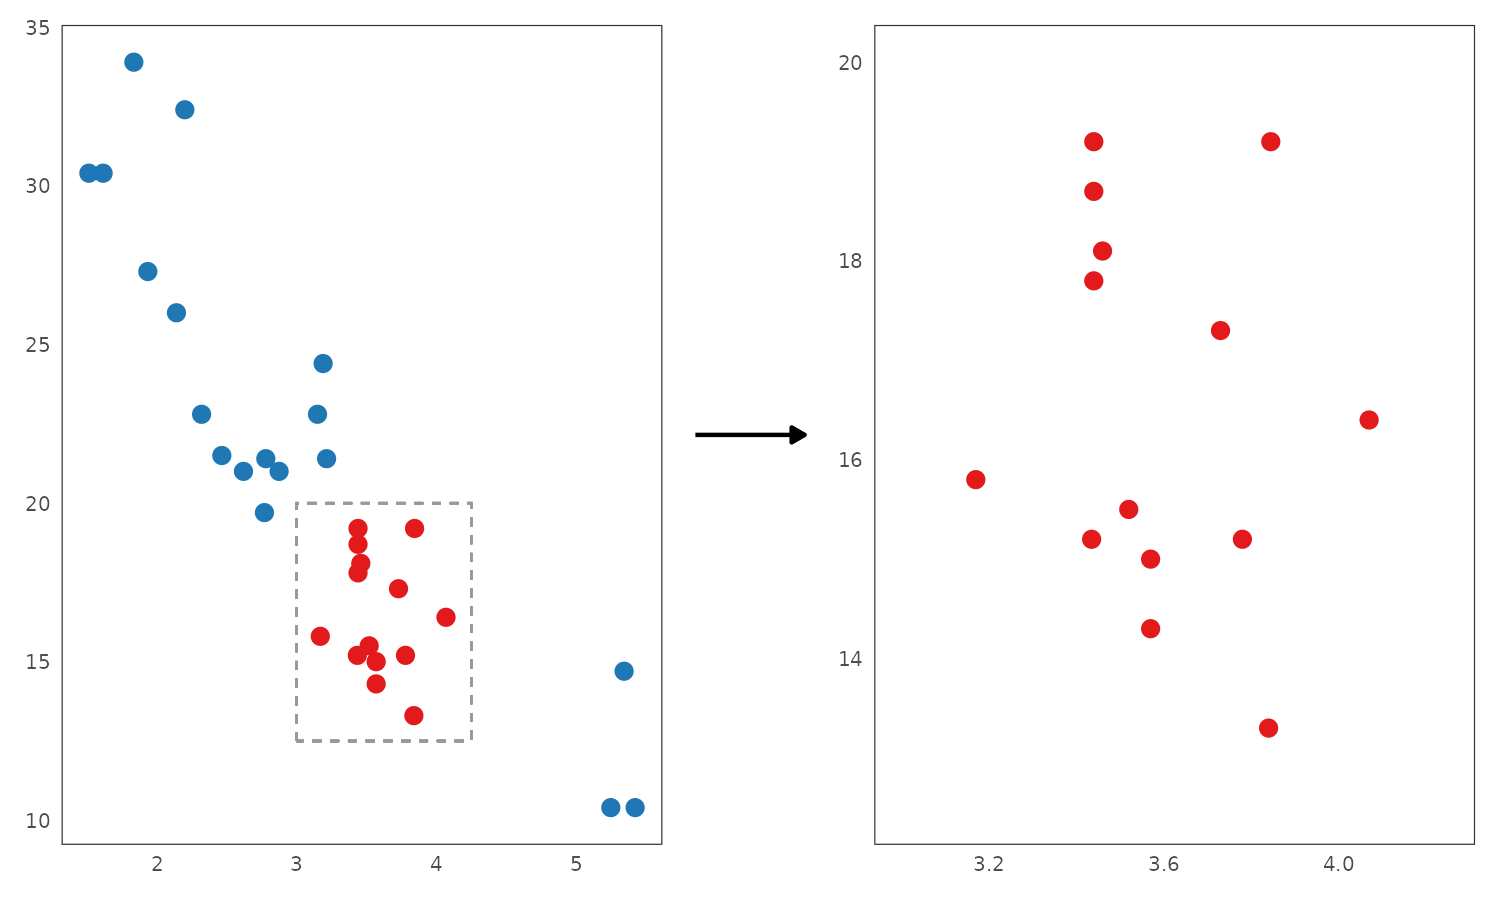
\includegraphics[width=1\linewidth,height=1\textheight]{./figures/zooming} 

}

\caption{Zooming involves shrinking the axis limits to obtain a more detailed view of the data. Typically, the user selects a rectangular region of the plot (left) and the plot scales are then adjusted so that the region fills up the entire plot area (right). Notice the change in the axis limits.}\label{fig:zooming}
\end{figure}

After zooming, it is useful to retain the ability to navigate the wider plot region while preserving the current zoom level and aspect ratio. Panning addresses this need. By performing some action, typically right-click and drag, the user can move the center of the zoomed-in region around, exploring different areas of the plot.

\begin{figure}

{\centering 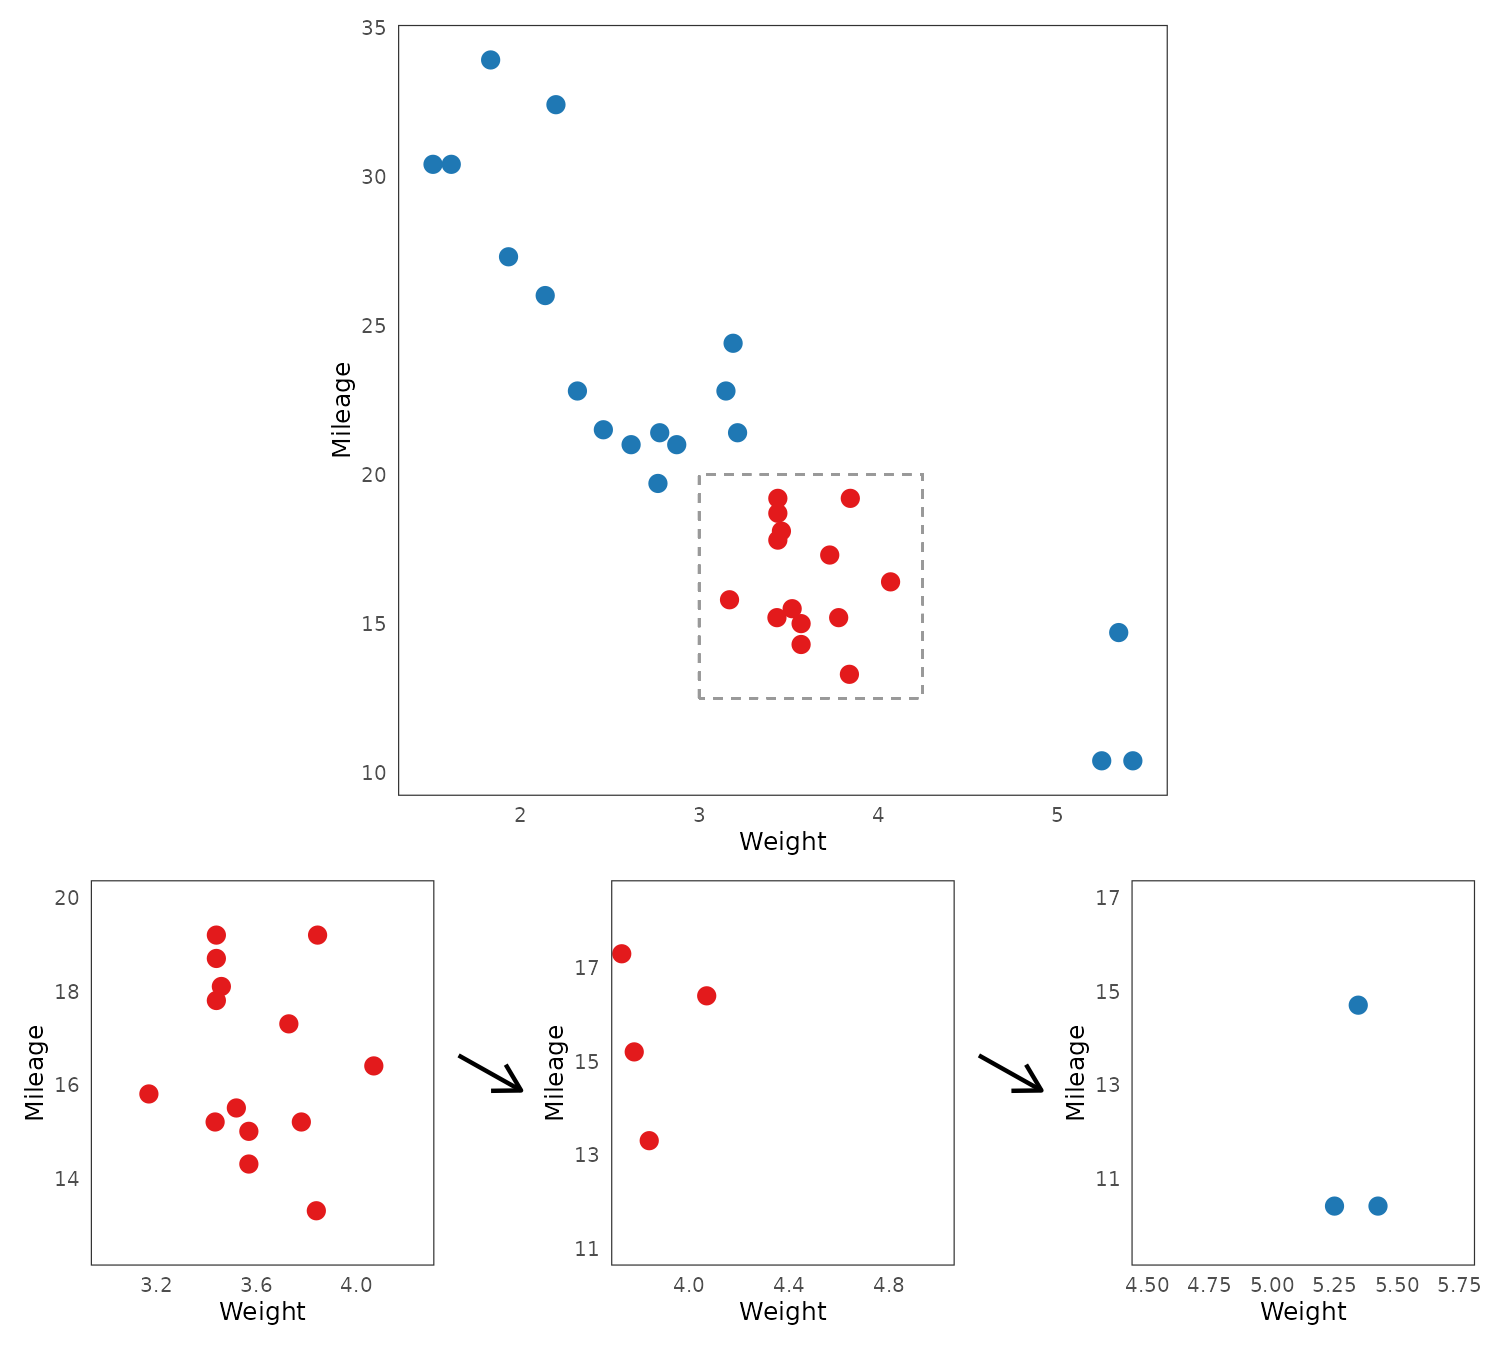
\includegraphics[width=1\linewidth,height=1\textheight]{./figures/panning} 

}

\caption{Panning involves moving the axis limits while retaining the same zoom level and axis ratio. After zooming into a rectangular region (top row), the user can around the plot region, usually by clicking and dragging (bottom row).}\label{fig:panning}
\end{figure}

Zooming and panning can be implemented by manipulating scales only, and this also makes them generally fairly straightforward to implement, similar to changing size and opacity. However, there are a few issues to consider. First, whereas continuous axes can be be zoomed and/or panned by simply modifying the axis limits, zooming discrete axes requires a bit more nuance (see e.g. \citeproc{ref-wilkinson2012}{Wilkinson 2012}). Second, it is often desirable to give the user the ability to zoom-in multiple levels deep, and this makes maintaining a reversible history of previous zoom-states essential (\citeproc{ref-unwin1999}{Unwin 1999}). Third, at times, it can be useful to link scale updates across multiple plots, such that, for example, zooming or panning a plot in a scatterplot matrix produces the same actions in other plots with the same variable on one of the axes. Finally, an advanced feature that can be also quite useful is semantic or logical zooming (\citeproc{ref-keim2002}{Keim 2002}; \citeproc{ref-unwin1999}{Unwin 1999}; \citeproc{ref-yi2007}{Yi et al. 2007}). This technique goes beyond magnifying objects; it also increases the level of detail the objects display as the user zooms in. Semantic zooming can be particularly powerful when combined with hierarchical data such as geographic information, however, it also introduces additional complexity, since the effects of the zoom action propagate beyond x- and y-axis scales.

\subsubsection{Querying}\label{querying}

Querying is another popular interactive feature that is usually fairly straightforward to implement. As shown in Figure \ref{fig:querying}, the way querying is typically implemented is that when a user mouses over a particular geometric object, a small table of key-value pairs is displayed via a tool-tip/pop-up, showing a summary of the underlying data point(s) (\citeproc{ref-urbanek2003}{Urbanek and Theus 2003}; \citeproc{ref-xie2014}{Xie, Hofmann, and Cheng 2014}). This makes it possible to look up precise values that would otherwise be available only approximately via the visual representation.

\begin{figure}

{\centering 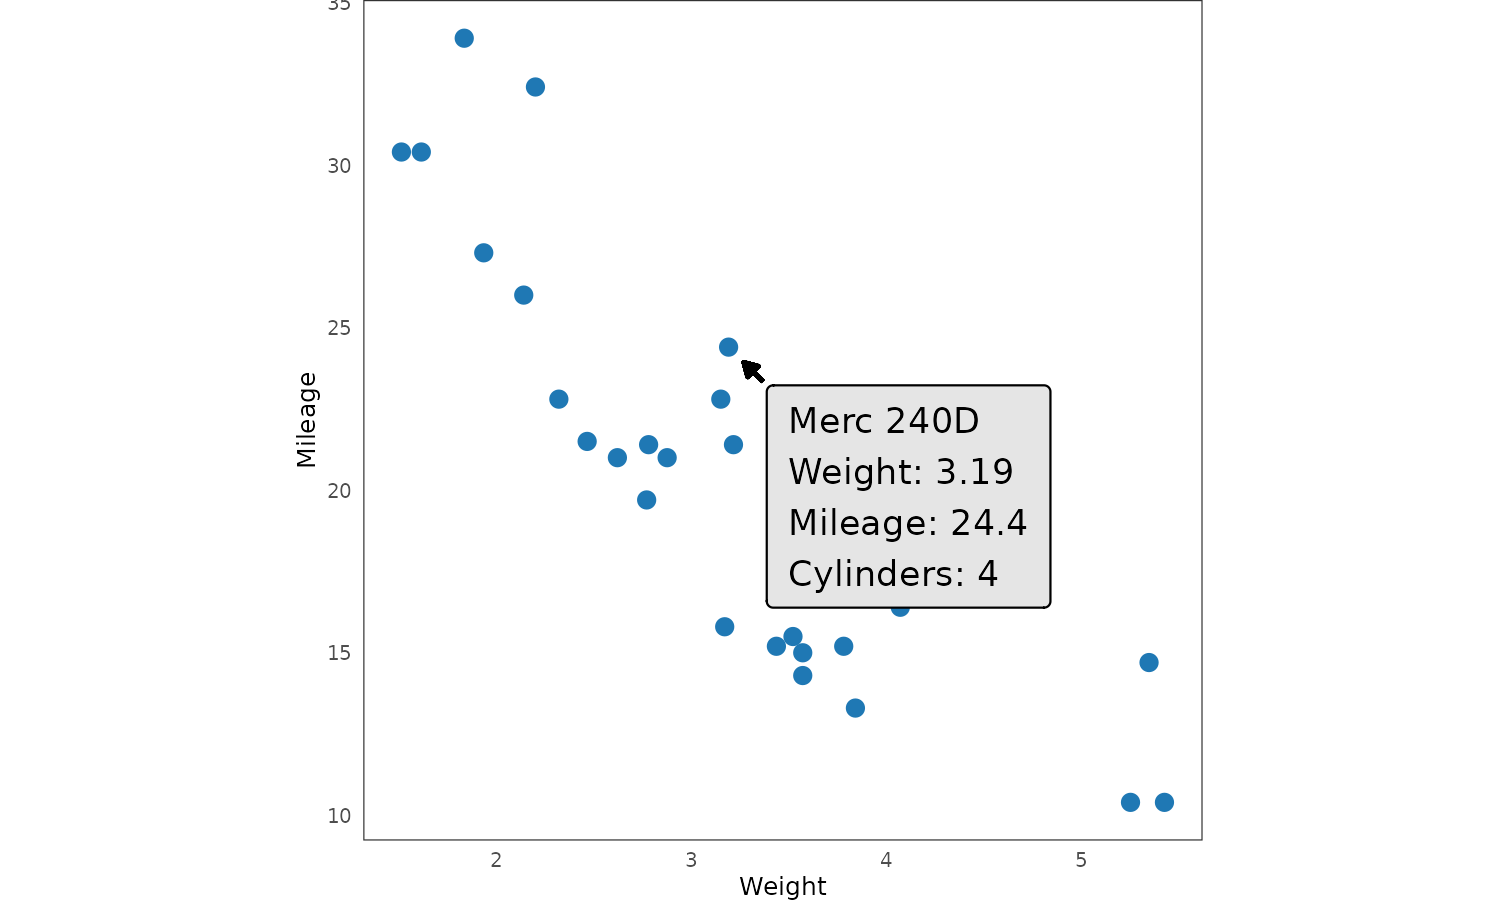
\includegraphics[width=1\linewidth,height=1\textheight]{./figures/querying} 

}

\caption{Querying involves hovering over an object to display its associated data values in a table or pop-up. Notice that this can include both plotted values (`weight`, `mileage`) as well as values that are not directly represented in the plot (car name, `cylinders`).}\label{fig:querying}
\end{figure}

Querying is useful because it combines the best features of graphics and tables. Specifically, it allows the user to overcome Tukey's famous prescriptions: ``graphics are for the qualitative/descriptive {[}\ldots{]} never for the carefully quantitative (tables do that better)'', and: ``graphics are for comparison {[}\ldots{]} not for access to individual amounts'' (\citeproc{ref-tukey1993}{Tukey 1993}). By providing the option to query individual objects, the user can seamlessly transition between the high-level analytic overview of the graphic and low-level quantitative detail of a table. This facilitates high-precision analytic tasks, such as identifying specific outliers or calculating exact magnitudes of differences (\citeproc{ref-unwin2006}{Unwin et al. 2006}).

Additionally, querying also allow us to show more information than is displayed via the visual encodings alone (see again Figure \ref{fig:querying}). Specifically, whereas most plots can encode only two or three variables, we can assign an arbitrary number of key-value pairs to the rows of the query table/pop-up. However, it is crucial to balance the level of detail against visual clutter. Too many rows may overtax the attention of the user and also can lead to clipping/overplotting issues, if the query table cannot fit inside the plotting area. Further, there are \hyperref[bidirectional-communication]{better methods} for retrieving very detailed information from interactive visualizations.

Finally, while querying is also one of the more straightforward features, its implementation does present certain challenges. First, a naive implementation might simply display derived data values in the state just before they are mapped to visual attributes via scales, however, these are not always the most informative. For instance, in a stacked barplot, returning the original (unstacked) values is more useful than the stacked ones. Second, aggregate plots such as barplots or histograms do generally present some design decisions (see \citeproc{ref-unwin2006}{Unwin et al. 2006}). In the case of one-to-one plots such as scatterplots, query data for an object (point) can be obtained by simply retrieving the corresponding row. However, in aggregate plots like barplots and histograms, a single object may correspond to multiple rows. This necessitates summarizing the underlying data, and often there may be no single ``correct'' summary. For instance, when querying a bar in a barplot, should we return the sum of the underlying continuous variable, some other numeric summary such as the mean or maximum, the set of all unique values, multiple of these summaries, or perhaps something else entirely? Similar ambiguities arise when querying objects which are partially selected or highlighted (see Section \ref{linked-selection}): should the query return summaries corresponding to the entire object, the highlighted parts, or both?

\subsubsection{Sorting and reordering}\label{sorting-and-reordering}

With plots of discrete (unordered) data, a highly useful feature can be to sort or reorder objects based on some criterion (see \citeproc{ref-unwin2000}{Unwin 2000}; \citeproc{ref-unwin2006}{Unwin et al. 2006}). For example, with barplots, in the absence of other ordering rules, bars are typically ordered by the lexographical order of the x-axis variable. However, sometimes, we can glean interesting patterns by sorting the bars in some other order, for example by their height, see Figure \ref{fig:sorting}.

\begin{figure}

{\centering 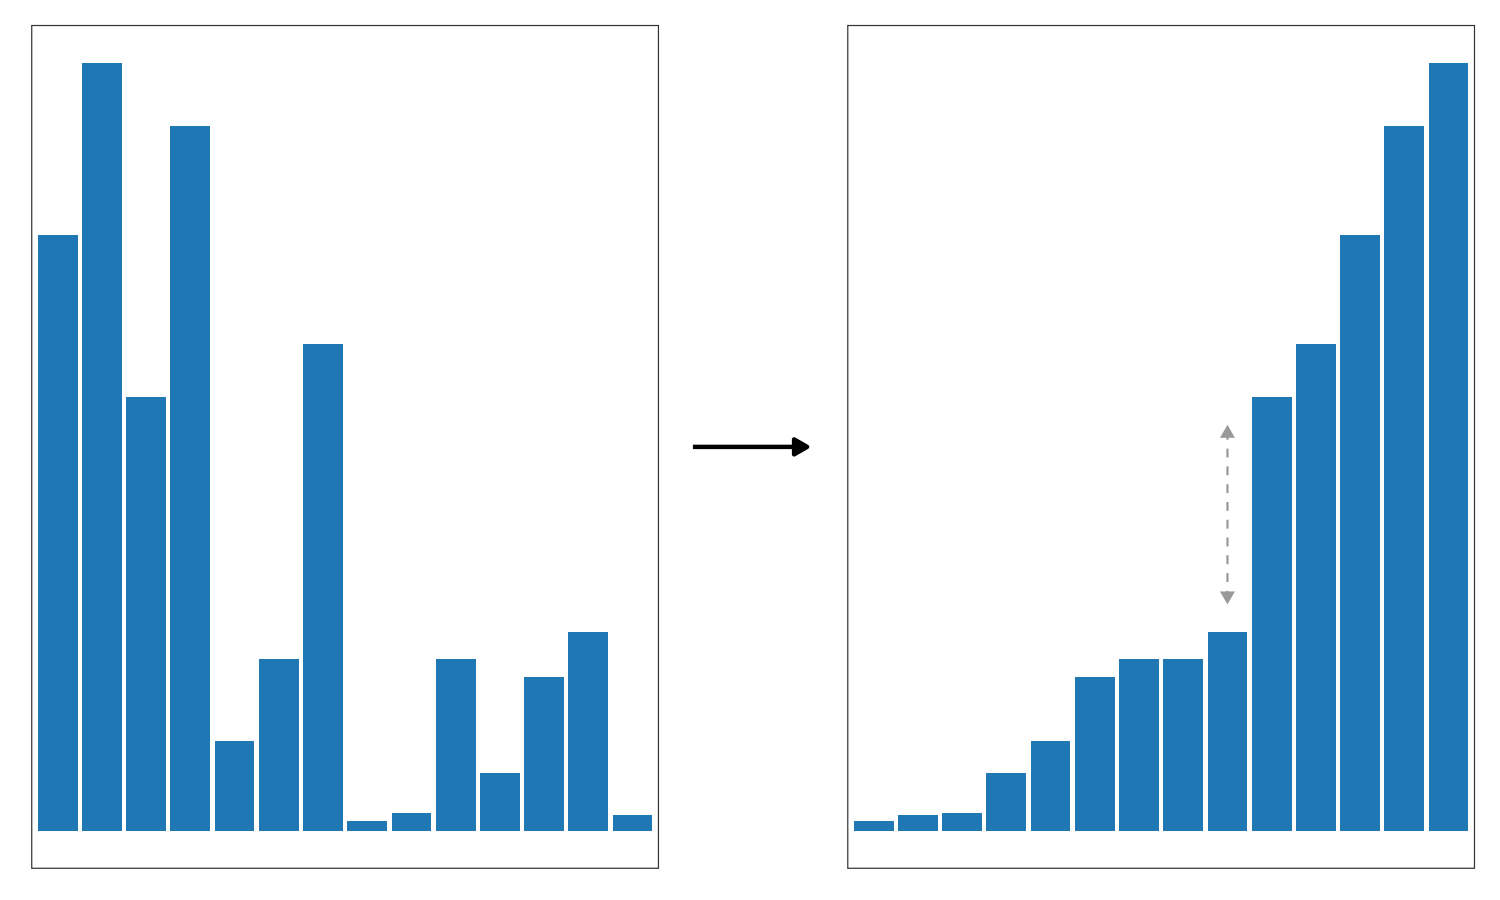
\includegraphics[width=1\linewidth,height=1\textheight]{./figures/sorting} 

}

\caption{Sorting or reordering can highlight interesting trends. For instance, sorting lexicographically ordered bars (left) by bar height (right) in the figure above immediately reveals a significant gap between the five tallest bars and the rest (gray dashed line).}\label{fig:sorting}
\end{figure}

There are more sophisticated ways to sort objects in a plot than just sorting bars by height, however. For instance, in plots which show multiple summary statistics, any may serve as the basis for the sorting rule; for instance a boxplot may be sorted by the median, upper and lower quartile, the maximum, and the minimum (\citeproc{ref-unwin2006}{Unwin et al. 2006}). Likewise, in the presence of selection/highlighting, objects may be sorted by the summary statistic on the highlighted parts. Alternatively, some systems allow users to permute the order of discrete scales manually by swapping the position of categories pairwise, a feature which can be particularly useful in parallel coordinate plots (\citeproc{ref-unwin2006}{Unwin et al. 2006}; \citeproc{ref-urbanek2011}{Urbanek 2011}). Finally, in the presence of many categories, sorting may also be usefully combined with lumping categories below a certain threshold together (\citeproc{ref-unwin2000}{Unwin 2000}).

Like zooming and panning, basic sorting typically involves the manipulation of axis scales only, making it also a fairly straightforward feature to implement. However, the more sophisticated sorting features can pose non-trivial implementation challenges (\citeproc{ref-unwin2006}{Unwin et al. 2006}). For instance, sorting by custom summary statistics or manually permuting discrete scale order may require specialized system components and behavior.

\subsubsection{Parametric interaction}\label{parametric-interaction}

As discussed in Section \ref{complexity-of-features}, another valuable class of interactive features are those which affect the computation of the summary statistics underlying the graphic (also called ``parametric interaction,'' \citeproc{ref-leman2013}{Leman et al. 2013}; \citeproc{ref-self2018}{Self et al. 2018}; \citeproc{ref-urbanek2011}{Urbanek 2011}). These features extend beyond simple manipulation of visual attributes, requiring that user interaction penetrates much deeper into the data visualization pipeline. Fundamentally, these features involve the manipulation of the parameters of some underlying mathematical model or algorithm.

An illustrative and popular example of parameter manipulation is dynamically changing histogram binwidth or anchor. Assuming a fixed binwidth \(w\) and an anchor \(a\), we can describe a histogram via a function \(h\) that, for each observation of a continuous variable \(x_i\) returns an index \(j\) of the corresponding bin, such that, for an ordered list of bins breaks \(b_j\), we have \(x_i \in [b_{j}, b_{j + 1})\)\footnote{Technically, if there are any values \(x_i < a\), we will have negative indices (\(j < 0\)), and if all values are significantly larger than the anchor, such that \(x_i > a + w\), the indices will not start at 1. So, to implement the histogram properly, we should shift all indices by subtracting the minimum index. Finally, if the histogram binwidth is not fixed, \(h\) becomes more complex as well.}:

\[h(x_i; a, w) = \lfloor (x_i - a) / w \rfloor + 1\]

Thus, a histogram really is a kind of a mathematical model, and can in fact be seen as a crude form of density estimation (see e.g. \citeproc{ref-bishop2006}{Bishop and Nasrabadi 2006, 4:120--22}). Manipulating histogram bins amounts to manipulating the parameters of the function \(h\). Crucially, unlike changes to surface-level visual attributes like size or opacity, changing binwidth or anchor requires recomputing the underlying summary statistics (\citeproc{ref-urbanek2011}{Urbanek 2011}). As noted in Section \ref{complexity-of-features}, these changes can have significant downstream effects. For instance, increasing the binwidth may cause certain bins to contain more data points than the current maximum, potentially requiring the adjustment of the upper y-axis limit, to prevent the bars from overflowing the plotting area.

There are other, more complex types of parametric interaction, than just changing histogram binwidth or anchor. These include, for example, modifying the bandwidth of a kernel density estimator, specifying the number of clusters in a clustering algorithm, or manipulating splitting criteria in classification and regression trees, as well as regularization parameters in smooth fits (for some more examples, see \citeproc{ref-leman2013}{Leman et al. 2013}; \citeproc{ref-self2018}{Self et al. 2018}).

Because parametric interaction necessitates recalculating the plot's underlying summary statistics, it is both more computationally expensive and as well as more difficult to implement. The interactive system must be able to respond to user input by recomputing relevant summaries and updating dependent plot parameters. In some systems such as Shiny (\citeproc{ref-shiny2024}{W. Chang et al. 2024}), the common approach is to re-render the entire plot from scratch each time any interaction occurs. However, this can become prohibitively expensive when these deep, parametric interactions are combined with rapid interactions closer to the surface of the visualization pipeline. Thus, the development of generic and efficient data visualization pipelines still remains an open research problem (\citeproc{ref-wickham2009}{Wickham et al. 2009}; \citeproc{ref-vanderplas2020}{Vanderplas, Cook, and Hofmann 2020}; \citeproc{ref-xie2014}{Xie, Hofmann, and Cheng 2014}).

\subsubsection{Animation and projection}\label{animation-and-projection}

A particularly useful form of parametric interaction involves the ability to control a continuous traversal through a series of states, observing the resulting changes as animation. This technique is especially useful when combined with projective techniques such as the grand tour (see \citeproc{ref-chen2008}{Chen et al. 2008}; for a recent comprehensive review, see \citeproc{ref-lee2022b}{Lee et al. 2022}), and for this reason I discuss them both here, within the same subsection.

A common and straightforward application of interactive animation is visualizing transitions in data subsets ordered by a specific variable, such as time. A particularly famous example of this technique is the \href{https://www.gapminder.org/tools/\#$chart-type=bubbles&url=v2}{interactive animation of the Gapminder data set} (\citeproc{ref-rosling2011}{Rosling and Zhang 2011}), which illustrates the joint evolution of GDP and life expectancy for countries worldwide. The interactive control of the timeline (play, pause, and pan) empowers users to explore time-dependent trends within this relatively high-dimensional data set, revealing trends that would be challenging to visualize by other means. For instance, the visualization clearly depicts the profound drop in both GDP and life expectancy during the second world war, followed by the subsequent rapid recovery and growth after 1945.

Interactive animation becomes particularly powerful when coupled with techniques like the grand tour (\citeproc{ref-asimov1985}{Asimov 1985}; \citeproc{ref-buja1986}{Buja and Asimov 1986}; \citeproc{ref-cook1995}{Cook et al. 1995}), designed for exploring high-dimensional datasets. Because data visualizations are typically limited to two dimensions, effectively representing high-dimensional data is challenging. The grand tour technique addresses this issue by projecting the data onto a series of lower-dimensional (two-dimensional) subspaces, interpolating between these projections, and animating the results to create a ``tour'' of different data views (\citeproc{ref-cook1995}{Cook et al. 1995}). By surveying this series of projections, the users may discover high-dimensional outliers, clusters, or non-linear dependencies (\citeproc{ref-wickham2011}{Wickham 2011}), and this discovery can be greatly aided by interactive controls of the animation's timeline or even manual control of the tour's direction (\citeproc{ref-chen2008}{Chen et al. 2008}; \citeproc{ref-lee2022b}{Lee et al. 2022}). Finally, the technique also integrates well with other interactive features, such as linked selection and querying/tooltips (\citeproc{ref-cook1995}{Cook et al. 1995}; \citeproc{ref-wickham2011}{Wickham 2011}; \citeproc{ref-lee2022a}{Lee, Laa, and Cook 2022}; \citeproc{ref-lee2022b}{Lee et al. 2022}).

The implementation complexity of interactive animation varies considerably depending on its application. While animating data subsets based on a single variable, as in the Gapminder visualization (\citeproc{ref-rosling2011}{Rosling and Zhang 2011}), presents no greater implementation challenges than previously discussed techniques, computing the grand tour path requires specialized algorithms (see, e.g., \citeproc{ref-chen2008}{Chen et al. 2008}, for a brief description). However, if the data subsets corresponding to each animation frame are pre-computed, the animation itself is generally fairly straightforward to implement.

\subsubsection{Representation switching}\label{representation-switching}

Another specialized kind of parametric (or semi-parametric) interaction involves changing the representation of the underlying data. It is well known that the same data can often be visualized using various sets of visual encodings (\citeproc{ref-wilkinson2012}{Wilkinson 2012}), with some being more effective for answering specific questions than others. Enabling users to switch between these various representations provides greater flexibility for data exploration (\citeproc{ref-yi2007}{Yi et al. 2007}). However, for certain plot types, changing the representation involves more than just altering surface-level visual attributes; it also necessitates recalculating derived statistics.

A typical example is switching between a barplot and a spineplot, see Figure \ref{fig:barplot-spineplot1}. Barplots are effective for comparing absolute quantities. Specifically, by encoding categories along the x-axis and continuous quantities along the y-axis (bar height), we can easily compare the quantities across categories. Color-coding parts of the bars as segments allows us to visualize a second categorical variable, enabling subgroup comparisons of absolute values. However, barplots are less well-suited for comparing the \emph{proportions} represented by these segments, particularly when bar heights vary considerably.

\begin{figure}

{\centering 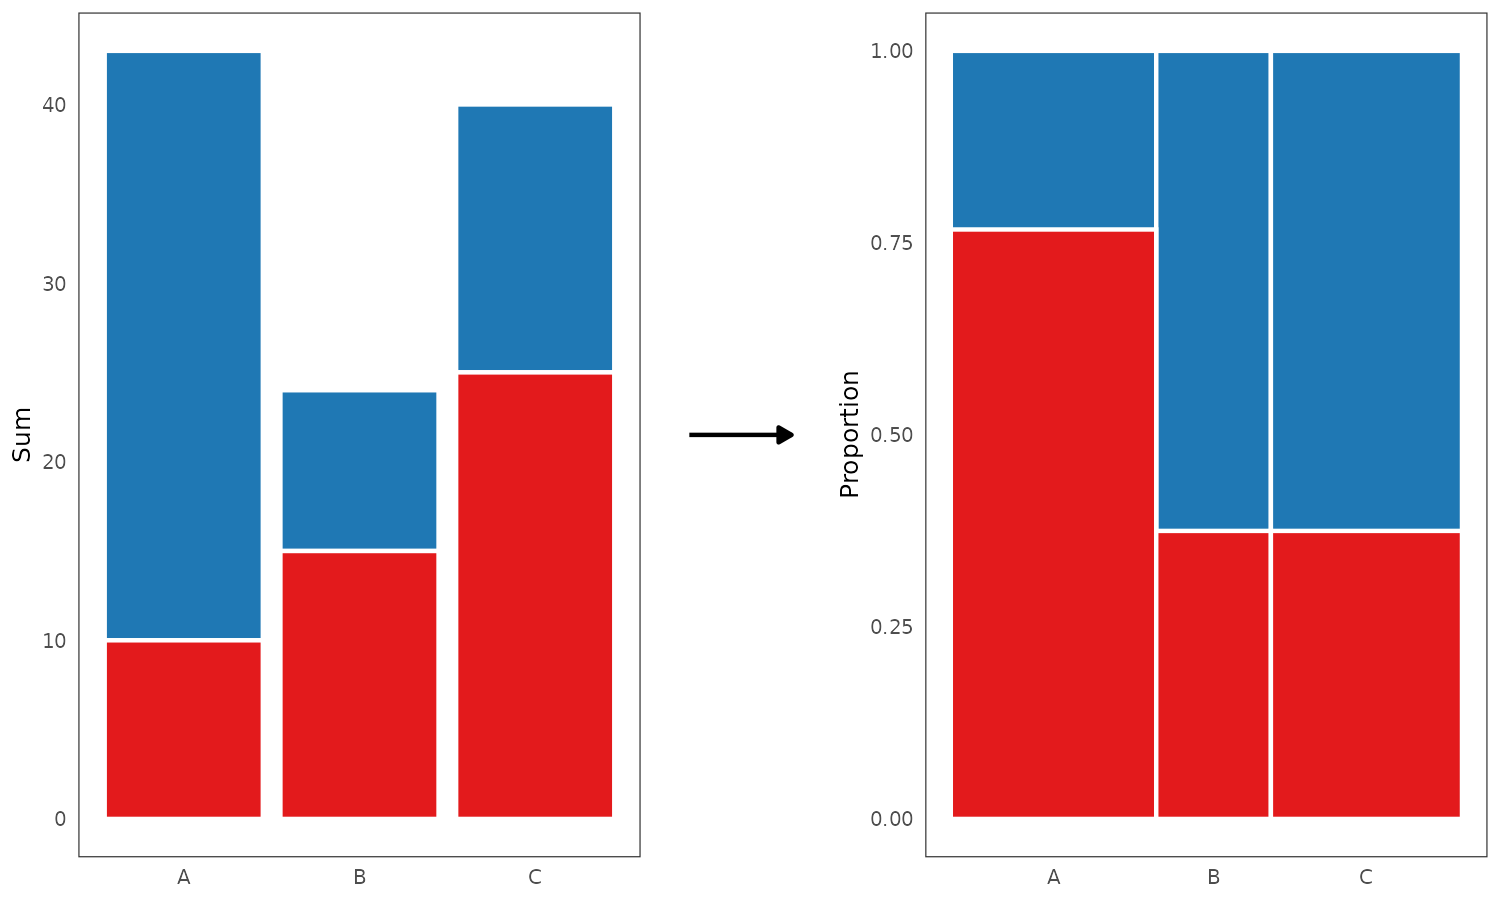
\includegraphics[width=1\linewidth,height=1\textheight]{./figures/barplot-spineplot} 

}

\caption{Switching representation can be an effective way to derive new insights from the data. A barplot (left) represents the same underlying data as a spineplot (right), however, the former is better for comparing absolute counts whereas the latter is better for comparing proportions. Note that in the spineplot, it is much easier to see that the proportion of the red cases is the same in categories B and C.}\label{fig:barplot-spineplot1}
\end{figure}

Spineplots, on the other hand, present a way of visualizing the same sort of data as a barplot while making it much easier to compare proportions. Specifically, in a spineplot, the heights of the bars are all normalized to 1, such that the segments show a proportion of the total, and the original values are instead encoded as the bar width, which is stacked along the x-axis. Thus, the fixed height of bars makes it easy to compare the segments proportionally.

Other examples of switching of representations include switching from a histogram to spinogram (a normalized version of the histogram) and switching between aggregate geometric objects and individual points (e.g.~boxplot, parallel coordinate plots).

\subsubsection{Linked selection}\label{linked-selection}

Linked selection, also known as linked brushing, linked highlighting, or linked views, is often considered one of the most versatile and powerful interactive data visualization features (see e.g. \citeproc{ref-becker1987}{Becker and Cleveland 1987}; \citeproc{ref-buja1996}{Buja, Cook, and Swayne 1996}; \citeproc{ref-wilhelm2003}{Wilhelm 2003}; \citeproc{ref-heer2012}{Heer and Shneiderman 2012}; \citeproc{ref-ward2015}{Ward, Grinstein, and Keim 2015}; \citeproc{ref-ware2019}{Ware 2019}). Fundamentally, it involves creating a figure with multiple ``linked'' plots. The user can then click or click-and-drag over objects in one plot, and the corresponding cases are highlighted across all the other plots, see Figure \ref{fig:linked-selection}. This makes it possible to quickly quickly explore trends across different dynamically-generated subsets of the data (\citeproc{ref-dix1998}{Dix and Ellis 1998}). The ability to quickly materialize alternative views of the data makes this a particularly effective tool for data exploration (\citeproc{ref-wilhelm2008}{Wilhelm 2008}; \citeproc{ref-wills2008}{G. Wills 2008}).

\begin{figure}

{\centering 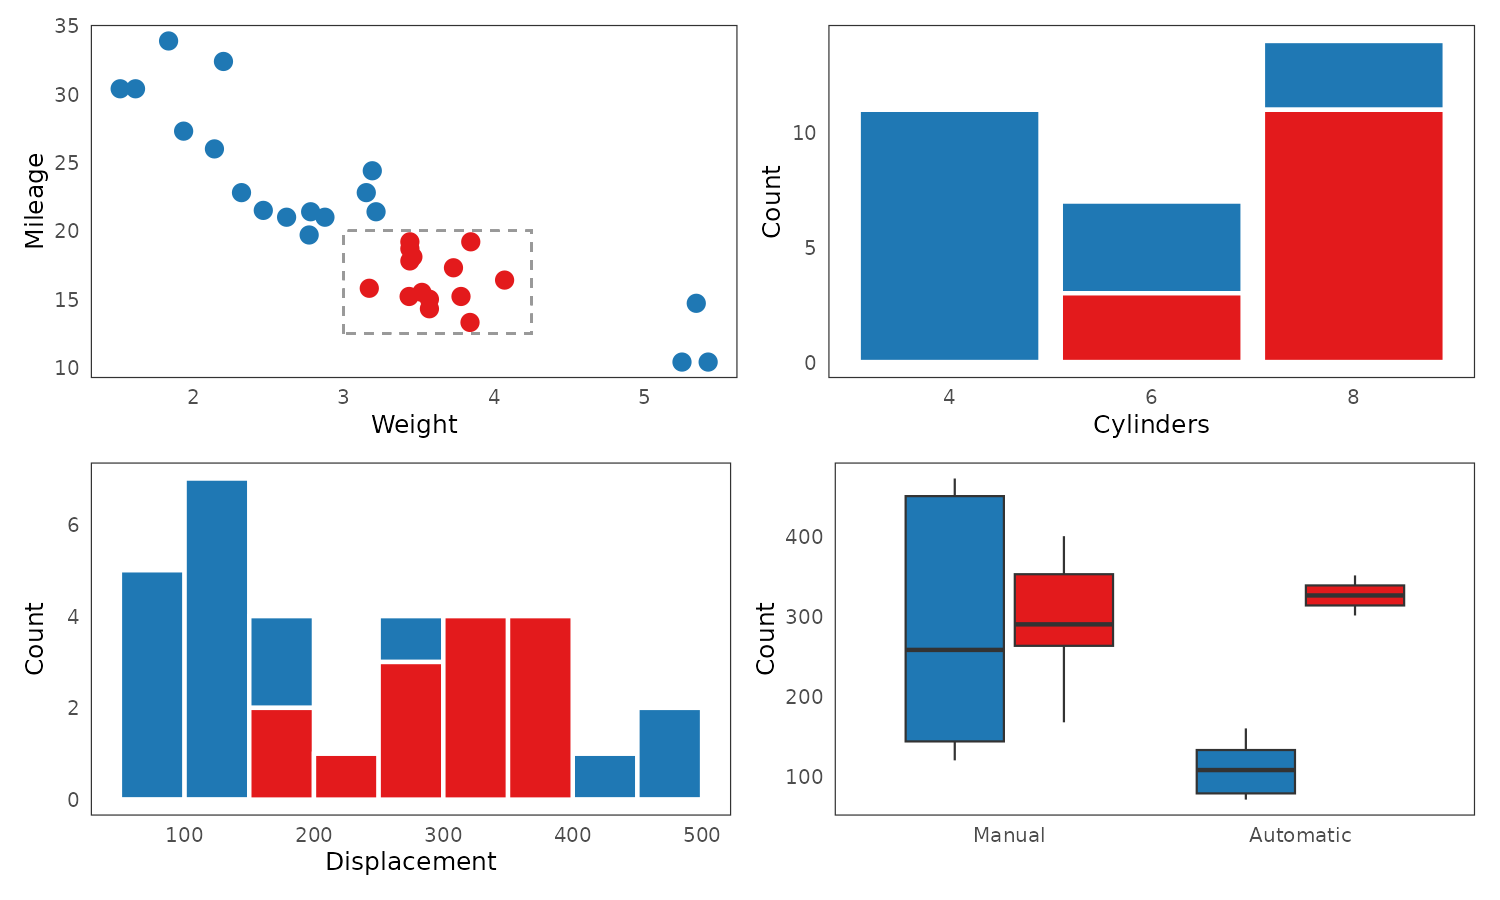
\includegraphics[width=1\linewidth,height=1\textheight]{./figures/linked-selection} 

}

\caption{Linked selection involves highlighting the same cases across all plots. The user can select some objects in one plot, such as points in a scatterplot (top left), and the corresponding cases are higlighted in all the other plots. Source of the underlying data is the `mtcars` dataset [@henderson1981].}\label{fig:linked-selection}
\end{figure}

Despite the fact that the user experience of linked selection is usually fairly intuitive, there are many subtle considerations that go into implementing the feature (for a good overview, see \citeproc{ref-wilhelm2008}{Wilhelm 2008}). First, there is the issue of how the user makes the selection. Typically, clicking selects a single objects and clicking-and-dragging selects multiple objects in a rectangular region (similar to how selecting files and folders works on desktop GUIs of most operating systems). In some systems, the users may also drag the selection region around (``brushing''), form a continuous ``lasso'' selection, select lines in a particular angular range, or points at a particular distance from a centroid (see e.g. \citeproc{ref-hauser2002}{Hauser, Ledermann, and Doleisch 2002}; \citeproc{ref-splechtna2018}{Splechtna et al. 2018}; \citeproc{ref-wills2008}{G. Wills 2008}). Further, when one variables is continuous and the other is derived (such as the x- and y-axes in a histogram), the interaction may also be simplified by restricting selection/brushing to the primary axis (\citeproc{ref-satyanarayan2016}{Satyanarayan et al. 2016}). Finally, the selections can be combined by various operators such as OR, AND, NOT, and XOR, to form unions, intersections, and other types of logical subsets (\citeproc{ref-theus2002}{Theus 2002}; \citeproc{ref-urbanek2003}{Urbanek and Theus 2003}; \citeproc{ref-wills2000}{G. J. Wills 2000}; \citeproc{ref-wills2008}{G. Wills 2008}).

Second, there is the issue of who should dispatch and respond to selection events. In presentation-focused interactive data visualization and dashboarding systems, this responsibility is kept flexible, such that some plots may only dispatch, only respond, do both, or neither (\citeproc{ref-satyanarayan2015}{Satyanarayan et al. 2015}, \citeproc{ref-satyanarayan2016}{2016}). However, in systems focused on data exploration, the convention is typically for all plots to both dispatch and respond to selection events, such that they may be interacted with in the same way. (\citeproc{ref-theus2002}{Theus 2002}; \citeproc{ref-urbanek2003}{Urbanek and Theus 2003}; \citeproc{ref-urbanek2011}{Urbanek 2011}).

Third, there is the issue of what to link. In the case of data represented by a two-dimensional table or data frame, the most common method is to link cases taken on the same observational level (identity linking), such that each row gets assigned a value representing the selection status (\citeproc{ref-urbanek2003}{Urbanek and Theus 2003}; \citeproc{ref-wilhelm2008}{Wilhelm 2008}; \citeproc{ref-wills2008}{G. Wills 2008}). However, in the case of more complex data, more advanced linking schemes are also available, such as hierarchical and distance-based linking (\citeproc{ref-wilhelm2008}{Wilhelm 2008}; \citeproc{ref-urbanek2011}{Urbanek 2011}).

Third, there is the issue of displaying selection. This issue will be touched upon in more detail later, in Section \ref{problems}. Briefly, Wilhelm (\citeproc{ref-wilhelm2008}{2008}) identifies three methods for displaying linked selection: replacement, overlaying, and repetition. Replacement involves replacing the entire plot with a new graphic; overlaying involves superimposing the objects representing the selected subsets on top of the original objects; and repetition involves displaying the selected objects alongside the original ones. Wilhelm identifies issues with all three techniques, although he does seem to generally come down in favor of repetition (however, see my argument in Section \ref{stacking-part-whole}).

A fourth and final issue in linked selection, and arguably one of the core concerns of the present thesis, is consistency. This topic will be coming up again and again, particularly in Section \ref{problems}. Consistent and predictable features are a cornerstone of good user interface design (see e.g. \citeproc{ref-ruiz2021}{Ruiz, Serral, and Snoeck 2021}). However, as discussed above, the design an interactive data visualization system supporting linked selection presents many design decisions, each with its own set of implementation constraints. Achieving a consistent user interface through the right combination of these decisions is a known challenge (\citeproc{ref-urbanek2011}{Urbanek 2011}; \citeproc{ref-pike2009}{Pike et al. 2009}).

For example, while the approach of allowing objects to independently dispatch and display selection events offers great flexibility, it can also lead to a less intuitive user experience. Put simply, when users select objects in one linked plot by clicking them, they might reasonably expect the same functionality in other plots. If that is not the case (if, for instance, other plots support only displaying but not dispatching selection events), their expectation will be violated. Thus, it might be reasonable to require that all objects can both dispatch and display selection events. However, this places some fundamental constraints on these objects. For instance, how do we draw a lineplot line where only some of the underlying cases are selected? Do we draw a sequence of differently-coloured line segments, leading to a striped ``candy cane'' pattern (see Figure \ref{fig:line-consistency})? Do we draw two separate lines? If so, how do we then dispatch selection events on these lines which are already conditional on selection? Like turning over a rock and disturbing a host of creepy-crawlies, linked selection reveals a complex web of visualization design challenges that defy a satisfying, generic solution.

\begin{figure}

{\centering 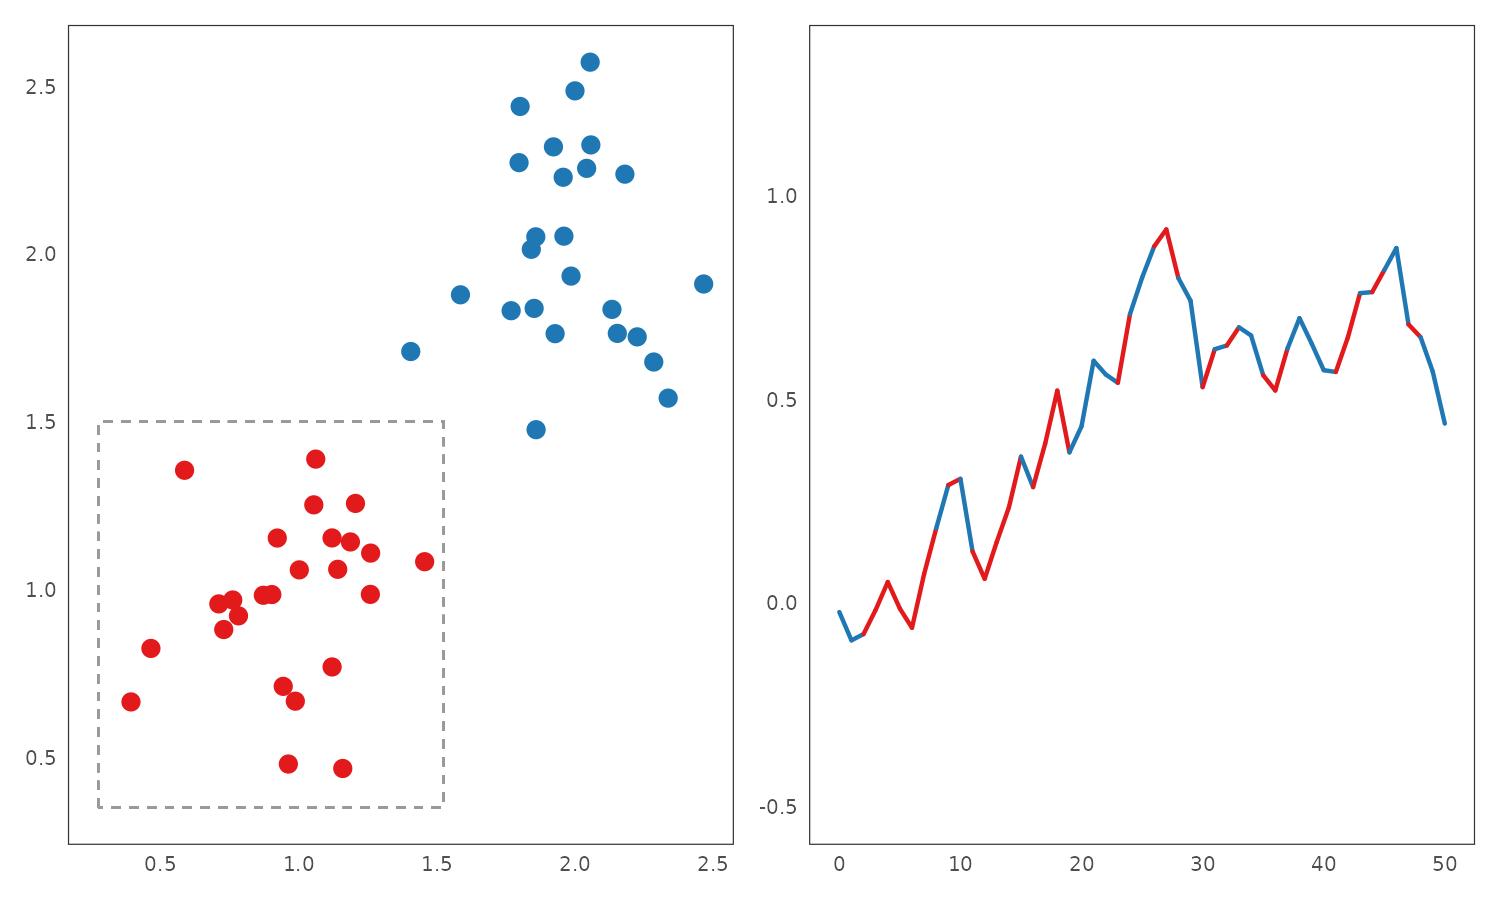
\includegraphics[width=1\linewidth,height=1\textheight]{./figures/line-consistency} 

}

\caption{Displaying selection is not always trivial. A good example is a lineplot (right). Whereas a point in a scatterplot displays a single case (row) and a bar in a barplot displays a simple subset of cases, a line segment in a lineplot connects two data points. As such, it is not clear whether to highlight the segment *starting* at the selected point, *ending* at the selected point, or, e.g., half a segment on each side of the point. Further, since the geometry of a segmented line is not commutative (row order matters), we end up with a striped 'candy cane' pattern that is not easily interpretable.}\label{fig:line-consistency}
\end{figure}

\section{General data visualization theory}\label{general-data-visualization-theory}

The following sections briefly explore several key theoretical topics in data visualization: the goals and purpose of visualizations, the mechanisms of visual perception, and the theory of scales and measurement. While mainly discussed in the context of static visualization, these topics are equally relevant to interactive visualization and present some unique challenges. My goal is not to give an exhaustive review - each of these topics is substantial enough to serve as a thesis topic in its own right. Instead, I just want to give a brief overview of these topics, highlight some key points, and discuss how they may relate to my own work.

\subsection{Visualization goals}\label{visualization-goals}

An important fact about data visualization is that, fundamentally, a chart can be used by many different people for many different things (for a review, see e.g. \citeproc{ref-brehmer2013}{Brehmer and Munzner 2013}; \citeproc{ref-franconeri2021}{Franconeri et al. 2021}; \citeproc{ref-sarikaya2018}{Sarikaya et al. 2018}). For example, applied researchers may create figures as part of their workflow, aiming to better understand the data they had collected, spot errors and anomalies, and come up with new ideas and hypotheses (\citeproc{ref-brehmer2013}{Brehmer and Munzner 2013}; see also \citeproc{ref-kandel2012}{Kandel et al. 2012}). Conversely, data scientists and data analysts in the public and private sector may visualize already familiar data sets to communicate important information, drive decisions, or convince or persuade stakeholders (\citeproc{ref-sarikaya2018}{Sarikaya et al. 2018}). Finally, some figures may be created out of a sense of curiosity or for pure aesthetic enjoyment (\citeproc{ref-brehmer2013}{Brehmer and Munzner 2013}; \citeproc{ref-tufte2001}{Tufte 2001}). Depending on the end-goals of the user and the desired target audience, certain visualization techniques, methods, or styles may become more useful than others.

As mentioned in Section \ref{interactive-interacting}, much has been written about the goals and experiences a user might have while creating data visualizations. For instance, Brehmer and Munzner (\citeproc{ref-brehmer2013}{2013}) formalized a typology of abstract visualization tasks, based around three adverbs: \emph{why} is a task is performed, \emph{how} it is performed, and \emph{what} does it pertain to. In the \emph{why} part of their typology, they list the following reasons for why a user may engage in the process of visualizing data: to consume (present, discover, or enjoy), produce, search (lookup, browse, locate, and explore), and query (identify, compare, summarize). As another example, Pike et al. (\citeproc{ref-pike2009}{2009}) list the following high-level goals a user might have when interacting with a visualization: explore, analyze, browse, assimilate, triage, asses, understand, compare. And there are many other typologies and taxonomies of data visualization tasks and goals in the literature.

Personally, when it comes to classifying interactive data visualization goals, I prefer the following short list provided by Ward, Grinstein, and Keim (\citeproc{ref-ward2015}{2015}):

\begin{itemize}
\tightlist
\item
  Exploration: The user wants to examine a data set
\item
  Confirmation: The user wants to verify a fact or a hypothesis
\item
  Presentation: The user wants to use the visualization to convince or inspire an audience
\item
  Interactive presentation: The user wants to take the audience on a guided tour of key insights
\end{itemize}

I believe this list maps fairly well onto interactive data visualization systems found in the wild, such as the ones discussed in Section \ref{brief-history}. Specifically, as mentioned before, in the history of interactive data visualization, the earlier statistical systems seemed to primarily focus on exploration and confirmation, whereas the newer web-based systems seem to prioritize presentation. The interactive presentation category is interesting, since, I would argue, it is far more specific and less common than the other categories, however, by singling it out, Ward et al.~make an interesting point. By incorporating time and intentionality, sequential interactive presentations, such as those found in the Graphics section of the New York Times (\citeproc{ref-nytimes2025}{The New York Times Company 2025}), really are quite unique.

\subsection{Visual perception}\label{visual-perception}

Another important research topic in data visualization is visual perception. Specifically, given that we use visual attributes such as position, color, length, or area to encode various aspects of our data, researchers have tried to answer the question of how to use these attributes in a way that best leverages the human visual system. Fortunately, this research has been quite fruitful, yielding precise and actionable guidelines (for a review, see \citeproc{ref-franconeri2021}{Franconeri et al. 2021}; \citeproc{ref-quadri2021}{Quadri and Rosen 2021}).

A landmark work in this area has been that of Cleveland and McGill (\citeproc{ref-cleveland1984}{1984}). In this study, the authors conducted a series of empirical experiments in which they investigated people's ability to accurately judge quantities based on different visual encodings. They found that judgments based on position along a common scale were the most accurate, followed by length-based comparisons, and then angle-based comparisons.

The findings were later corroborated by other authors. Heer and Bostock (\citeproc{ref-heer2010}{2010}) replicated the Cleveland and McGill (\citeproc{ref-cleveland1984}{1984}) study, and included judgements of circular and rectangular areas which were found to be less accurate than position, length, or angle. Other authors have extended these experiments to other visual encodings, such as color or density (e.g. \citeproc{ref-demiralp2014}{Demiralp, Bernstein, and Heer 2014}; \citeproc{ref-saket2017}{Saket et al. 2017}; \citeproc{ref-reda2018}{Reda, Nalawade, and Ansah-Koi 2018}). Together, these findings have been used to create rankings of visual encodings, with researchers generally agreeing on the following ordered list: position, length, area, angle, and intensity (from most effective to least, \citeproc{ref-mackinlay1986}{Mackinlay 1986}; \citeproc{ref-franconeri2021}{Franconeri et al. 2021}; \citeproc{ref-quadri2021}{Quadri and Rosen 2021}).

\subsection{Scales and measurement}\label{scales-measurement}

Visualizing data involves mapping values to graphical attributes. As discussed in the previous section, certain visual attributes are better for visualizing particular types of data, and vice versa. However, even when we pick an appropriate visual attribute to represent our data with, there are still many choices in how to perform the mapping. For instance, suppose we have some variable \(x\) with values \(\{ 1, 2, 3 \}\). Should these be treated as magnitudes, a simple ordering, or even just category labels that may be permuted at will? In most data visualization systems, this metadata encoding of values into visual attributes is handled specialized components called scales or coordinate systems, and I will discuss their implementation in detail later, in Section \ref{scales-composition}. However, it is first necessary to discuss some theoretical issues involving scales.

A particular challenge when discussing scales in data visualization is that the topic unavoidably intersects with a research area that has a particularly long and contentious history: theory of measurement (see e.g. \citeproc{ref-hand1996}{Hand 1996}; \citeproc{ref-michell1986}{Michell 1986}; \citeproc{ref-tal2025}{Tal 2025}). Theory of measurement (not to be confused with measure theory, with which it nevertheless shares some overlap) is the research area which tries to answer the deceptively simple question: what does it mean to measure something? This seemingly trivial problem has inspired long and fiery debates within the fields of mathematics, philosophy, and social science. Particularly, in psychology, where assigning numerical values non-physical phenomena such as moods and mental states is a central concern, the topic has garnered a significant amount of attention, creating a dense body of research (see e.g. \citeproc{ref-humphry2013}{Humphry 2013}; \citeproc{ref-michell2021}{Michell 2021}).

Arguably, the most influential work in this field has been that of Stevens (\citeproc{ref-stevens1946}{1946}). In his fairly concise paper, Stevens defined a \emph{scale} as method of assigning numbers to values, and introduced a four-fold classification classification, namely: nominal, ordinal, interval, and ratio scales (see Table \ref{tab:stevens-scales}).

\begin{table}

\caption{\label{tab:stevens-scales}Types of scales identified by Stevens (1946)}
\centering
\begin{tabular}[t]{l|l|l|l}
\hline
Scale & Structure & Comparison & Valid transformations\\
\hline
Nominal & Isomorphism & Are \$x\$ and \$y\$ the same? & \$x' = f(x)\$, where \$f\$ is a bijection\\
\hline
Ordinal & Monotone map & Is \$x\$ is greater than \$y\$? & \$x' = f(x)\$, where \$f\$ is a monotone bijection\\
\hline
Interval & Affine transformation & How far is \$x\$ from \$y\$? & \$x' = ax + b\$, for \$a, b \textbackslash{}in \textbackslash{}mathbb\{R\}\$\\
\hline
Ratio & Linear map & How many times is \$x\$ greater than \$y\$? & \$x' = ax\$, for \$a \textbackslash{}in \textbackslash{}mathbb\{R\}\$\\
\hline
\end{tabular}
\end{table}

The Steven's (\citeproc{ref-stevens1946}{1946}) typology is based on invariance under transformation. Specifically, for each class of scales, we define a set of transformations that preserve valid comparisons. The set of valid transformations shrinks as we move from one class of scales to another.

For nominal scales, any kind of bijective transformation is valid. Intuitively, we can think of the scale as assigning labels to values, and any kind re-labeling is valid, as long as it preserves equality of the underlying values. For instance, given a nominal scale with three values, we can assign the labels \(\{ \text{red}, \text{green}, \text{blue} \}\) or \(\{ \text{monday}, \text{tuesday}, \text{wednesday} \}\) in any way we like, as long as each value maps to a unique label. This identifies the underlying mathematical structure as an isomorphism.

Ordinal scales are more restrictive, since, on top of preserving equality, transformations also need to preserve order. For example, if we want to assign the labels \(\{ \text{monday}, \text{tuesday}, \text{wednesday} \}\) to an ordinal scale with three values, there is only one way to do it that preserves the underlying order: assign the least values to \(\text{monday}\), the middle value to \(\text{tuesday}\), and the greatest value to \(\text{wednesday}\) (assuming we order the labels/days in the usual day-of-week order). However, there is no notion of distance between the labels: we could just as well assign the values labels in \(\mathbb{N}\) such as \(\{ 10, 20, 30 \}\), \(\{1, 2, 9999 \}\), and so on. Thus, the fundamental mathematical structure is that of a monotone map.

Interval scales need to additionally preserve equality of intervals. This means that, for any three values \(a, b,\) and \(c\), if the distances between \(a\) and \(b\) and \(b\) and \(c\) are equal, \(d(a, b) = d(b, c)\), then so should be the distances between the scaled labels, \(d^*(f(a), f(b)) = d^*(f(b), f(c)\). For most real applications, this limits interval scales to the class of affine transformations of the form \(f(x) = ax + b\). A canonical example of an interval scale is the conversion formula of degrees Celsius to Fahrenheit: \(f(c) = 9/5 \cdot c + 32\) (\citeproc{ref-stevens1946}{Stevens 1946}). This example also highlights an important property of interval scales: the zero point can be arbitrary and ratios are not meaningful. Specifically, since the zero points of both Celsius and Fahrenheit scales were chosen based on arbitrary metrics (freezing temperatures of water and brine, respectively), it does not make sense to say that, e.g.~20°C is ``twice as hot'' as 10°C, in the same way that it does not make sense to say that 2000 CE is ``twice as late'' as 1000 CE.

Finally, ratio scales also need to preserve the equality of ratios. Specifically, if \(a/b = b/c\) then \(f(a)/f(b) = f(b) / f(c)\). As a consequence, this also means that the scale must have a well-defined zero-point. Examples of ratio scales include physical magnitudes such as height and weight, which have a well-defined zero point (\citeproc{ref-stevens1946}{Stevens 1946}).

Steven's (\citeproc{ref-stevens1946}{1946}) typology sparked a considerable debate, on multiple fronts. First, since the original publication, many authors have sought to either expand upon or criticize Steven's typology. However, despite some monumental efforts towards a unified theory, such as that of Krantz et al. (\citeproc{ref-krantz1971}{1971}), measurement has remained a hotly debated topic to this day (see e.g. \citeproc{ref-michell2021}{Michell 2021}; \citeproc{ref-tal2025}{Tal 2025}). Second, more relevant to statistics, some authors such as Stevens (\citeproc{ref-stevens1951}{1951}) and Luce (\citeproc{ref-luce1959}{1959}) used the theory to define come up with prescriptive rules for statistical transformations, suggesting that, for example, taking the mean of an ordinal variable is wrong since the meaning of the average operator is not preserved under monotone transformations. However, this issue was hotly contested by statisticians such as Lord (\citeproc{ref-lord1953}{1953}), Tukey (\citeproc{ref-tukey1986}{1986}), and Velleman and Wilkinson (\citeproc{ref-velleman1993}{1993}), who argued that many well-established statistical practices, such as rank-based tests and coefficients of variations, rely on such ``impermissible'' statistics but can nevertheless yield valuable insights. More broadly, these authors also argued that data is not really meaningful on its own, but instead derives its meaning from the statistical questions it is used to answer (see also \citeproc{ref-wilkinson2012}{Wilkinson 2012}).

At this point, the discussion around measurement has arguably become far too dense and theoretical, and most data visualization researchers seem to avoid delving into it too deeply (see e.g. \citeproc{ref-wilkinson2012}{Wilkinson 2012}). Nevertheless, there are still some areas where the issues of measurement and Steven's typology do crop up. For instance, when scaling area based on a continuous variable, a common recommendation is to start the scale at zero to ensure accurate representations of ratios (see e.g. \citeproc{ref-wickham2024}{Wickham and Navarro 2024}), aligning with Steven's definition of a ratio scale. Likewise, the long-standing debate around whether the base of a barplot should always start at zero (see e.g. \citeproc{ref-cleveland1985}{Cleveland 1985}; \citeproc{ref-wilkinson2012}{Wilkinson 2012}) also carries echoes of the measurement debate. Ultimately, it may yet require long time to settle the issues around measurement, however, there are definitely some ideas within the literature that data visualization can benefit from.

\newcommand\thena{⨾}

\chapter{Challenges}\label{problems}

Designing an interactive data visualization system presents a unique set of challenges. Some of these have been already touched on in the Section \ref{litreview}. This section homes in on these inherent challenges, discusses them in greater depth, and begins exploring avenues for possible solutions.

\section{The structure of this chapter: Data visualization pipeline}\label{the-structure-of-this-chapter-data-visualization-pipeline}

When creating visualizations, be they static or interactive, our ultimate goal is to render geometric objects that will represent our data in some way. However, it is rarely the case that we can plot the raw data directly, as is. Instead, before the data can be rendered, it often has to pass through several distinct transformation steps or stages. Together, these steps form a data visualization pipeline (see e.g. \citeproc{ref-chi2000}{Chi 2000}; \citeproc{ref-wickham2009}{Wickham et al. 2009}; \citeproc{ref-wu2024}{Wu and Chang 2024}). Each of these steps come with its inherent set of considerations and challenges, particularly when interaction is involved.

Take, for instance, the typical barplot. There are several steps to drawing a barplot. First, we have to divide the data into subsets, based on the levels of some categorical variable. Second, we need to summarize or aggregate these subsets by some metric, usually either sum or count. Third, we need to take these summaries and map them to visual encodings, such as x-axis position, y-axis position, and length. Finally, we use these encodings and render the individual bars as rectangles on the computer screen (see e.g. \citeproc{ref-franconeri2021}{Franconeri et al. 2021}).

Thus, the data visualization pipeline can be described by four fundamental steps:

\begin{itemize}
\tightlist
\item
  Partitioning
\item
  Aggregation
\item
  Scaling/encoding
\item
  Rendering
\end{itemize}

These four steps are common to both static and interactive visualization systems, however, interactivity does introduce some unique challenges. User interaction may affect any of the four stages, and as a result, changes need to be propagated accordingly. Finding a general and efficient solution to this change-propagation remains an open research topic (\citeproc{ref-wickham2009}{Wickham et al. 2009}; \citeproc{ref-franconeri2021}{Franconeri et al. 2021}). Consequently, discussions of the role interaction within the data visualization pipeline are often fairly vague (see \citeproc{ref-dimara2019}{Dimara and Perin 2019}; \citeproc{ref-wu2024}{Wu and Chang 2024}).

This chapter attempts to clarify some of this conceptual ambiguity. Mirroring the structure of the data visualization pipeline, it delves into each of the four steps and explores challenges related to their implementation in interactive systems. The central argument is that interaction is not just a thin veneer that can be layered on top of static graphics; instead, it fundamentally penetrates the abstract machinery of the pipeline. Moreover, for interaction to be predictable, intuitive, and efficient, the components of the pipeline must compose together in specific, well-defined ways, that may be described algebraically using the language of category theory. Mapping out this algebraic composition is crucial for building truly generic and robust interactive data visualization systems (see also \citeproc{ref-wu2024}{Wu and Chang 2024}; \citeproc{ref-sievert2020}{Sievert 2020}).

\section{Partitioning}\label{partitioning}

The first step of any data visualization pipeline is to divide the data into parts or subsets. The justification for this initial step lies in our ultimate goal: to draw one or (usually) more geometric objects (\citeproc{ref-wilkinson2012}{Wilkinson 2012}; also known as graphic items, \citeproc{ref-wills2008}{G. Wills 2008}), representing some aspects of our data. Thus, before we can do anything else, we need to define the set of data points each geometric object will represent. In the typical case of two-dimensional tables or data frames, this amounts to slicing the table's rows into smaller sub-tables.

The partitioning operation is fairly intuitive for aggregate plots, where each object represents multiple rows of the data. For instance, in a barplot, each bar represents a set of cases corresponding to a category, while in histogram, each bar represents a set of cases in which fall within the same bin along some continuous dimension. However, even one-to-one representations of the data can be viewed this way. For example, in a scatterplot or parallel coordinate plots, each geometric object represents one row of the data, which we can view as its own small table. Similarly, plots with a single geometric object (e.g.~density/radar plots) have the underlying set equal to the whole data set.

Thus, the process of splitting our data into subsets is in some way fairly straightforward. However, it does raise two fundamental questions:

\begin{itemize}
\tightlist
\item
  How much of the original data should the subsets contain?
\item
  What should be the relations between the subsets?
\end{itemize}

While common data visualization practices provide implicit solutions to these questions, explicit formulations are rarely given in the data visualization literature. This lack of conceptual clarity is problematic because how we choose to partition our data is a consequential decision; when we split our data into subsets, we make assumptions, about the data itself as well as the goals of the visualization process. In interactive data visualization particularly, the relations between the parts of our data become of key importance. Therefore, discussing the two questions above in greater depth is essential.

\subsection{Showing the full data}\label{show-all-data}

\begin{quote}
``If someone hides data from you, it's probably because he has something to hide.'' (\citeproc{ref-cairo2016}{Cairo 2016, 47})
\end{quote}

A common recommendation that many data visualization experts provide is that faithful visual representations should show the full data and leave nothing out. The moral behind this recommendation is fairly intuitive. A visualization which hides or obscures information, be it by intent or negligence, cannot be considered a truthful representation of the underlying information (\citeproc{ref-cairo2016}{Cairo 2016}, \citeproc{ref-cairo2019}{2019}).

However, data hiding can occur in many different ways. First, the data itself can be cherry-picked or massaged (see e.g. \citeproc{ref-lisnic2024}{Lisnic et al. 2024}). This is arguably the most egregious case, and can in some cases amount to malicious statistical practices such as HARKing or p-hacking (see e.g. \citeproc{ref-kerr1998}{Kerr 1998}; \citeproc{ref-lisnic2024}{Lisnic et al. 2024}; \citeproc{ref-head2015}{Head et al. 2015}). However, even when showing the full data, some visualizations can obscure or downplay certain data features via poor design or incorrect use of visual encodings (\citeproc{ref-cairo2016}{Cairo 2016}, \citeproc{ref-cairo2019}{2019}; \citeproc{ref-cleveland1985}{Cleveland 1985}; \citeproc{ref-ziemkiewicz2009}{Ziemkiewicz and Kosara 2009}). Finally, there is the issue of missing or incomplete data, where some data cannot be easily represented because it is simply not there.

An infamous example of data hiding leading to disastrous real-world consequences was the 1986 crash of the Space Shuttle Challenger (see \citeproc{ref-dalal1989}{Dalal, Fowlkes, and Hoadley 1989}). During a pre-launch teleconference, engineers debated the effect of temperature on the performance of O-ring gaskets, as the forecasted temperature was significantly lower than during previous launches. The plot in the left panel of Figure \ref{fig:challenger} was used to argue that there was no correlation between temperature and O-ring failures. However, this plot had one significant flaw: it excluded launches where no failures occurred. After the disaster, when the data including the zero-failure launches was plotted, it revealed a clear trend of increasing number of failures as temperature decreased (see right panel of Figure \ref{fig:challenger}, see also \citeproc{ref-dalal1989}{Dalal, Fowlkes, and Hoadley 1989}).

\begin{figure}

{\centering 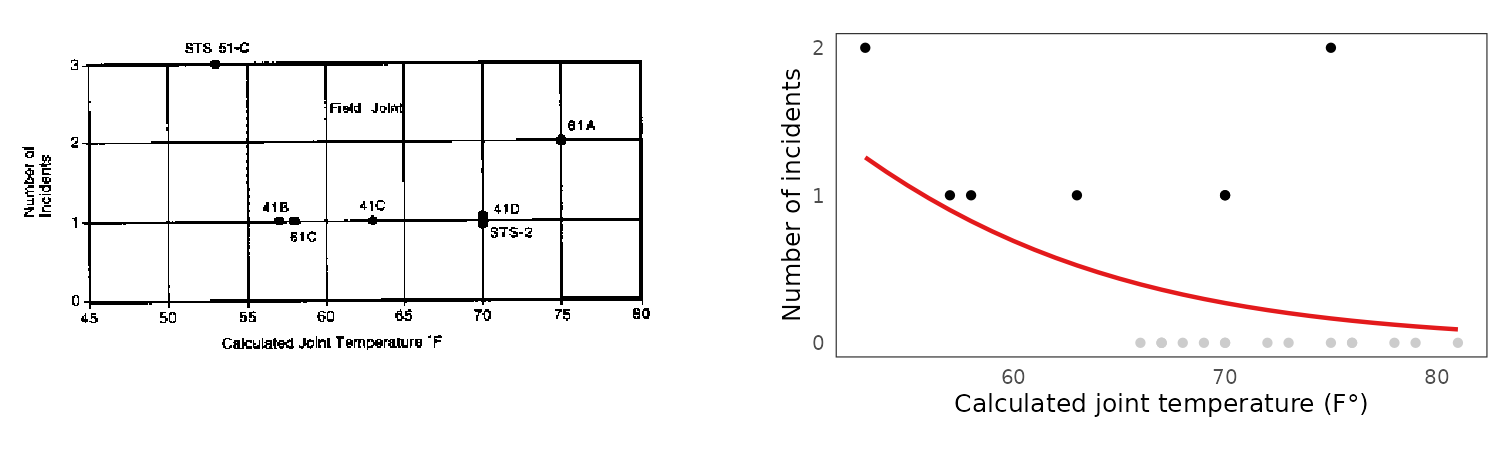
\includegraphics[width=1\linewidth,height=1\textheight]{./figures/challenger} 

}

\caption{Relationship between temperature and the number of O-ring failures within the 1986 Challenger data. Left: the original plot as presented during the pre-launch teleconference. Right: a reproduced plot of the same data, including the original data points (black), the excluded data points with zero failures (grey), and an estimated logistic regression fit (red). The source of right-panel data is @dalal1989.}\label{fig:challenger}
\end{figure}

However, data hiding can also occur in more subtle ways, such as the above-mentioned poor design choices. Consider, for example, axis limits. Cleveland (\citeproc{ref-cleveland1985}{1985}) argues that axis limits should generally be expanded to avoid inadvertently obscuring data near these limits (see also e.g. \citeproc{ref-chen2008}{Chen et al. 2008, 64}). Take the following two scatterplots:

\begin{figure}

{\centering 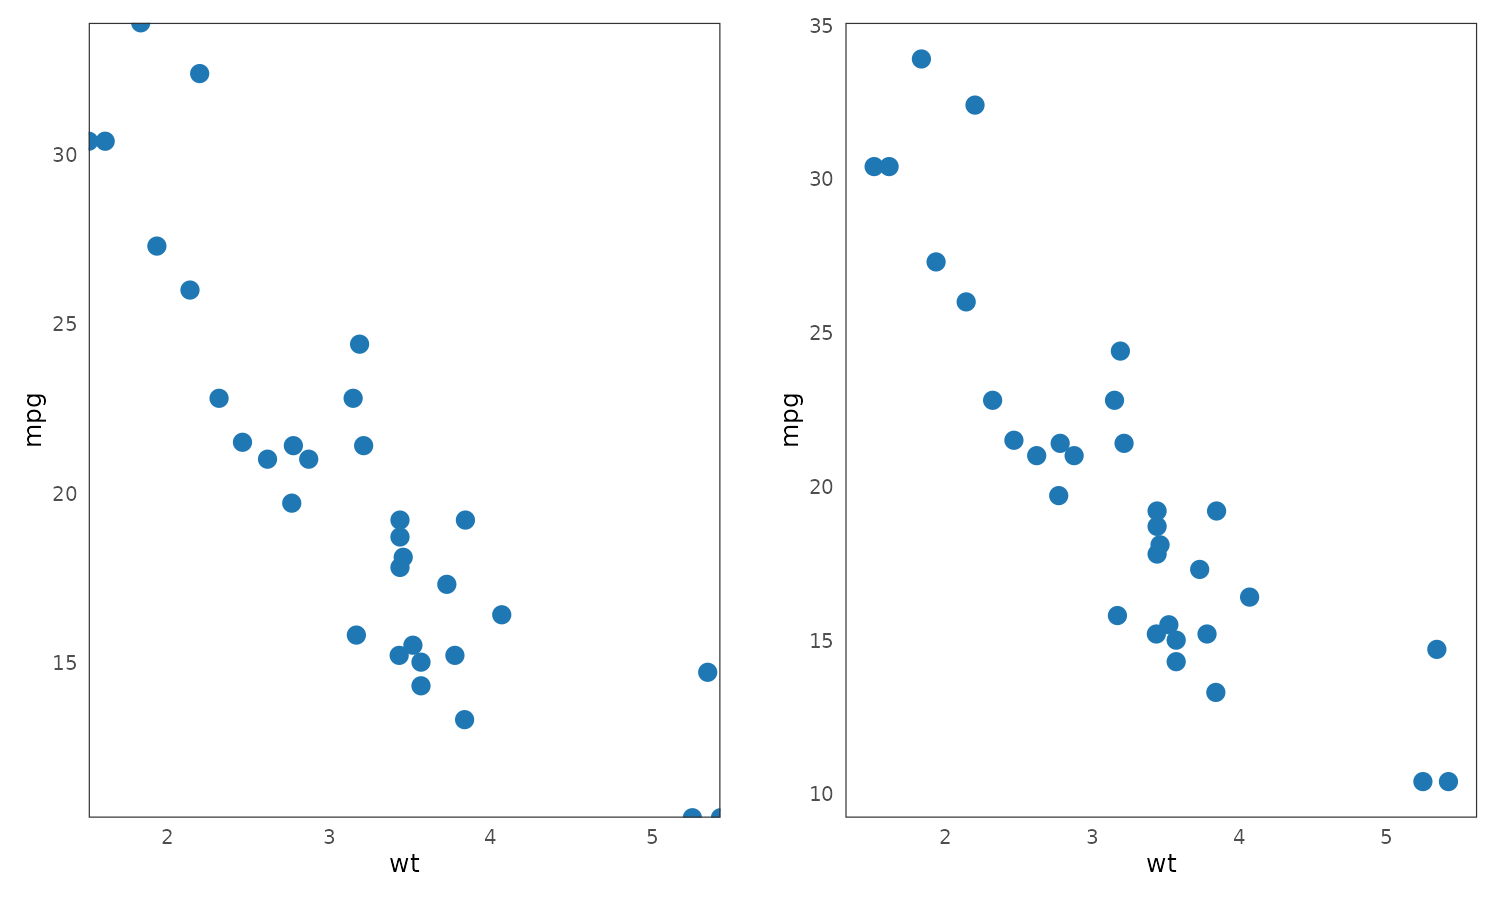
\includegraphics[width=1\linewidth,height=1\textheight]{./figures/expand-scatterplot} 

}

\caption{Without expanding axis limits, objects at or near the limits become less salient. Left: axis limits match the data limits exactly, and so the points in the top-left and bottom-right corner of the plot are represented by smaller area and the overall trend is distorted. Right: by expanding axis limits, we can ensure that trend is represented faithfully.}\label{fig:unnamed-chunk-13}
\end{figure}

In the left scatterplot, the axis limits match the data limits exactly, whereas in the right plot, they are expanded by a small fraction (5\%, \texttt{ggplot2} default, \citeproc{ref-wickham2016}{Wickham 2016}). The left scatterplot provides a misleading representation of the underlying trend, as data points near or at the axis limits (top-left and bottom-right corners) are represented by a smaller area, compared to points near the centre of the plot. For instance, the point in the bottom-right corner of the plot lies simultaneously at the limits of the x- and y-axis, and is thus represented by one-quarter of the area of the points in the center.

Finally, there is the issue of data hiding due to missing or incomplete data, which is a bit more complicated. While techniques of visualizing data with missing values do exist (see e.g. \citeproc{ref-unwin1996}{Unwin et al. 1996}; \citeproc{ref-tierney2023}{N. Tierney and Cook 2023}), they are often tied to specific visualization types and styles, and few general solutions are available. Properly analyzing the patterns of missingness in the data often calls for a full-fledged separate visualization workflow (\citeproc{ref-tierney2023}{N. Tierney and Cook 2023}).

Either way, data hiding is something we should be mindful of. Unless there is a clear and justifiable reason, no data should be arbitrarily removed or discarded, and we should pick good visual representations to represent all of our data faithfully. In the ideal case, the visualization should present a clear and unambiguous mapping between the graphics and the data (\citeproc{ref-ziemkiewicz2009}{Ziemkiewicz and Kosara 2009}).

\subsection{Disjointness and comparison}\label{disjointness-and-comparison}

\begin{quote}
``To be truthful and revealing, data graphics must bear on the question at the heart of quantitative thinking: `compared to what'?'' (\citeproc{ref-tufte2001}{Tufte 2001, 74}).
\end{quote}

\begin{quote}
``Graphics are for comparison - comparison of one kind or another - not for access to individual amounts.'' (\citeproc{ref-tukey1993}{Tukey 1993})
\end{quote}

An interesting yet underappreciated fact is that in many common visualization types, geometric objects tend to represent disjoint subsets of the data. That is, in most plots, each point, bar, line, or polygon corresponds a unique set of data points (rows of the data), with no overlap with other objects within the same graphical layer. While different layers can represent the same data (e.g., a smooth fit over a scatterplot, or point clouds over boxplots), objects within the same layer rarely represent the same data. This practice, despite being so common to border on a rule, it is surprisingly seldom discussed.

There are of course counter-examples. For instance, certain visualizations of set-typed data ``double up'' the contribution of data subsets, such that the same subset of the data may appear in multiple objects (see e.g. \citeproc{ref-alsallakh2013}{Alsallakh et al. 2013}, \citeproc{ref-alsallakh2014}{2014}; \citeproc{ref-conway2017}{Conway, Lex, and Gehlenborg 2017}; \citeproc{ref-lex2014}{Lex et al. 2014}). However, these types of visualizations are fairly rare, and represent the exception rather than the norm. When we see a barplot, we typically expect each bar to represent a unique set of cases.

But where does this unconscious ``law'' of showing disjoint parts of the data come from? I argue that it stems from the fundamental purpose of data visualization: comparison (\citeproc{ref-tufte2001}{Tufte 2001}; \citeproc{ref-tukey1993}{Tukey 1993}). When we visualize, we draw our graphics with the ultimate goal of comparing our data along a set of visual channels (\citeproc{ref-bertin1983}{Bertin 1983}; \citeproc{ref-wilkinson2012}{Wilkinson 2012}; \citeproc{ref-franconeri2021}{Franconeri et al. 2021}; \citeproc{ref-wilke2019}{Wilke 2019}). This mirrors the comparisons we make about objects and events in the real world. And, in general, it is far easier to reason about objects and events that are independent, rather than ones which overlap or blend together. One example of this comes from basic probability theory, where the sum and product rules have independence as a pre-requisite (\citeproc{ref-kolmogorov2018}{Kolmogorov and Bharucha-Reid 2018}). Similarly, psychological research, such as the well-known ``Linda experiment'' (\citeproc{ref-tversky1983}{Tversky and Kahneman 1983}), shows that people struggle with comparing the probability of non-disjoint events. Thus it seems that, in many ways, disjointness presents a more intuitive, ``natural'' model.

More fundamentally, disjointness may be more intuitive because it reflects a structure which mathematicians have long considered natural: a \hyperref[functions]{bijection} or one-to-one mapping (see e.g. \citeproc{ref-fong2019}{Fong and Spivak 2019}; \citeproc{ref-lawvere2009}{Lawvere and Schanuel 2009}). Specifically, if we take a set, split it into disjoint subsets, and label each subset, then there is a one-to-one correspondence between these subsets and the subset labels (i.e.~the parts form an \hyperref[partition]{equivalence class}). Practically, this means that we can go back and forth between the subsets and the corresponding labels, without losing any information.

The fact that disjoint subsets form a bijection may be particularly useful in data visualization and this may explain its ubiquity, see Figure \ref{fig:geoms-bijection}. For instance, when drawing a barplot, if we divide our data into disjoint subsets and draw one bar corresponding to each part, then we can go back and forth between identifying subsets of the data corresponding to individual bars and vice versa. Thus, the function of identifying data subsets is invertible. In plots where the objects do not represent disjoint subsets, this correspondence is broken: if we select a subset of cases corresponding to a bar, there may be no simple way to identify the original bar from the cases alone. This issue applies both conceptually, when viewing static visualizations, and also more practically, when interacting with interactive visualizations, via features such as linked selection.

\begin{figure}

{\centering 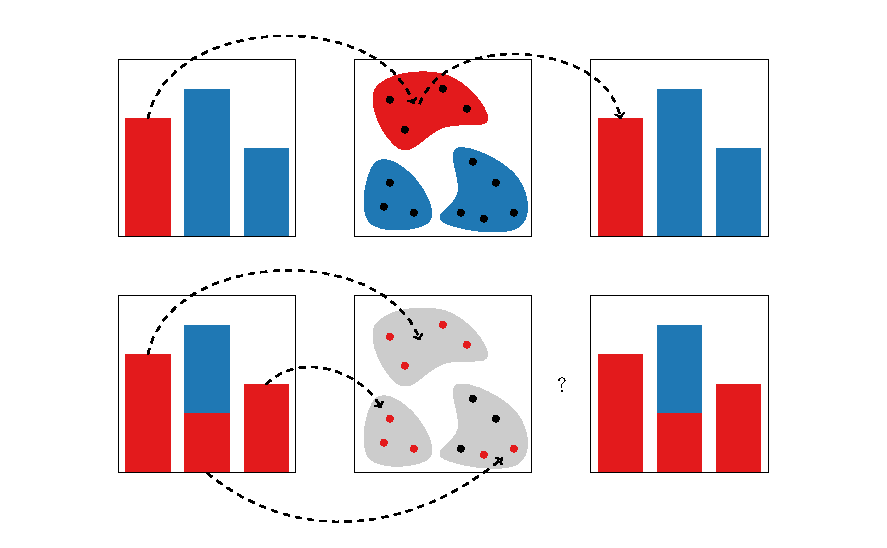
\includegraphics[width=1\linewidth,height=1\textheight]{./figures/geoms-bijection} 

}

\caption{Disjointness induces a one-to-one mapping (bijection) between geometric objects and subsets of the data. Suppose we mark out the cases corresponding to the leftmost bar (red). Top row: when each geometric object (bar) represents unique subset of data points, we can easily go back and forth between the object and its underlying subset (middle panel), and so the function of picking cases corresponding to each object is invertible. Bottom row: if there is an overlap between the cases represented by each object, then there may be no way to identify the original object after we have picked out the corresponding cases.}\label{fig:geoms-bijection}
\end{figure}

\subsubsection{Real-world example}\label{real-world-example}

To illustrate the idea of disjoint subsets on concrete, real-world example, take the following barplot representing the vote share among the top three parties in the 2023 New Zealand general election (\citeproc{ref-election2023}{Electoral Commission New Zealand 2023}):

\begin{figure}

{\centering 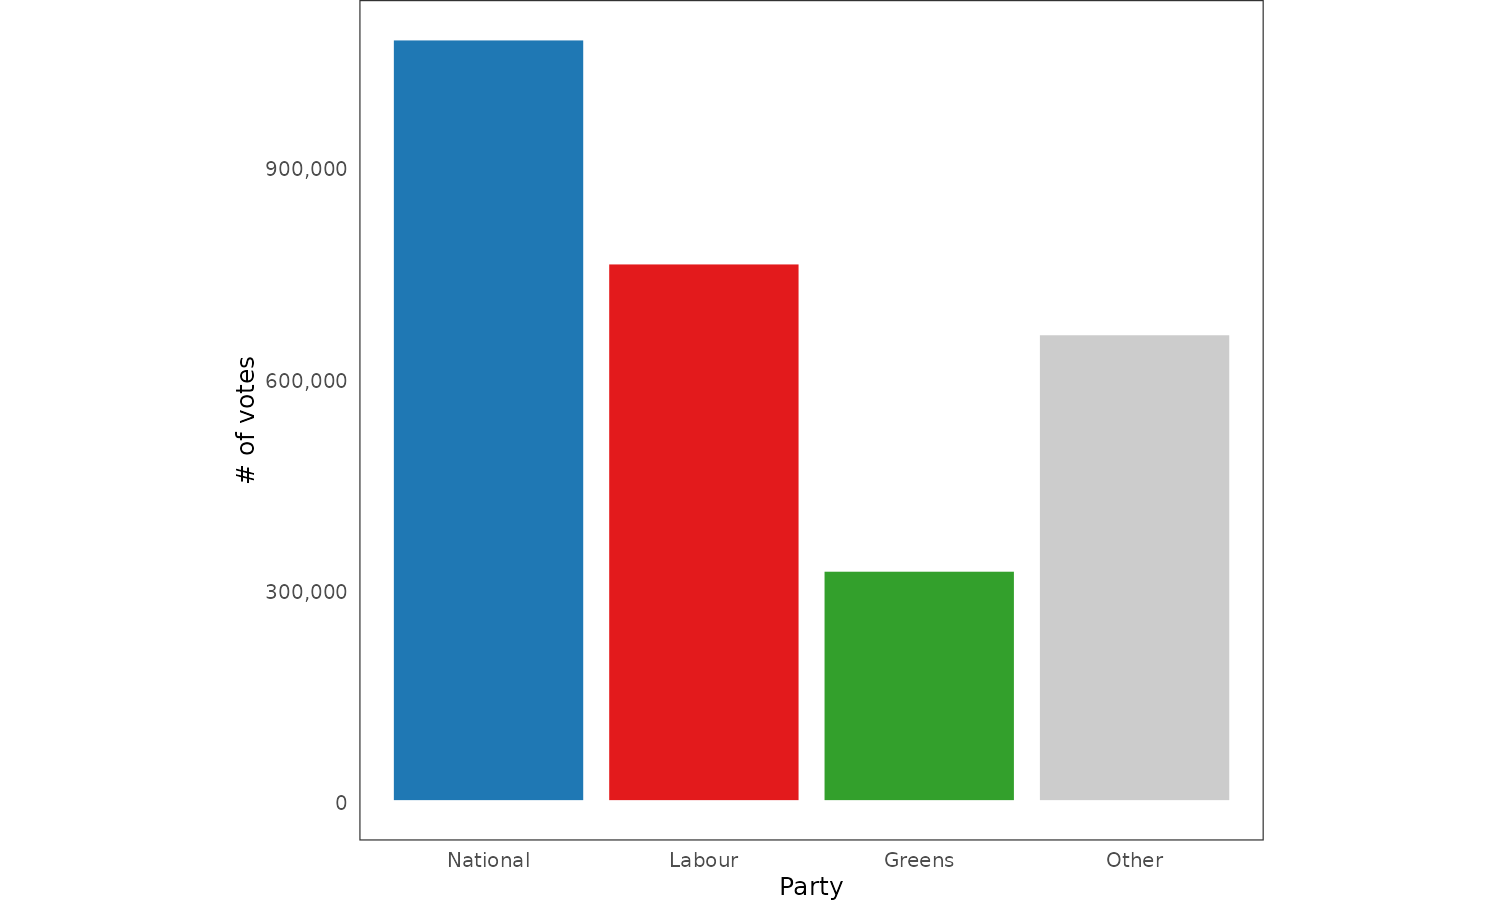
\includegraphics[width=1\linewidth,height=1\textheight]{./figures/barplot-bijection} 

}

\caption{Barplot showing disjoint subsets of the data. The bars show the vote share among the top three parties in the 2023 New Zealand general election, with each bar representing a unique subset of voters.}\label{fig:barplot-bijection}
\end{figure}

Each bar represents a unique subset of voters and thus the bars show disjoint data. This is the type of data representation that we encounter most often, however, there are few explicit guidelines about this. Hypothetically, we could transform our data, and use the leftmost bar to show, for example, the union of the votes of National and Labour parties:

\begin{figure}

{\centering 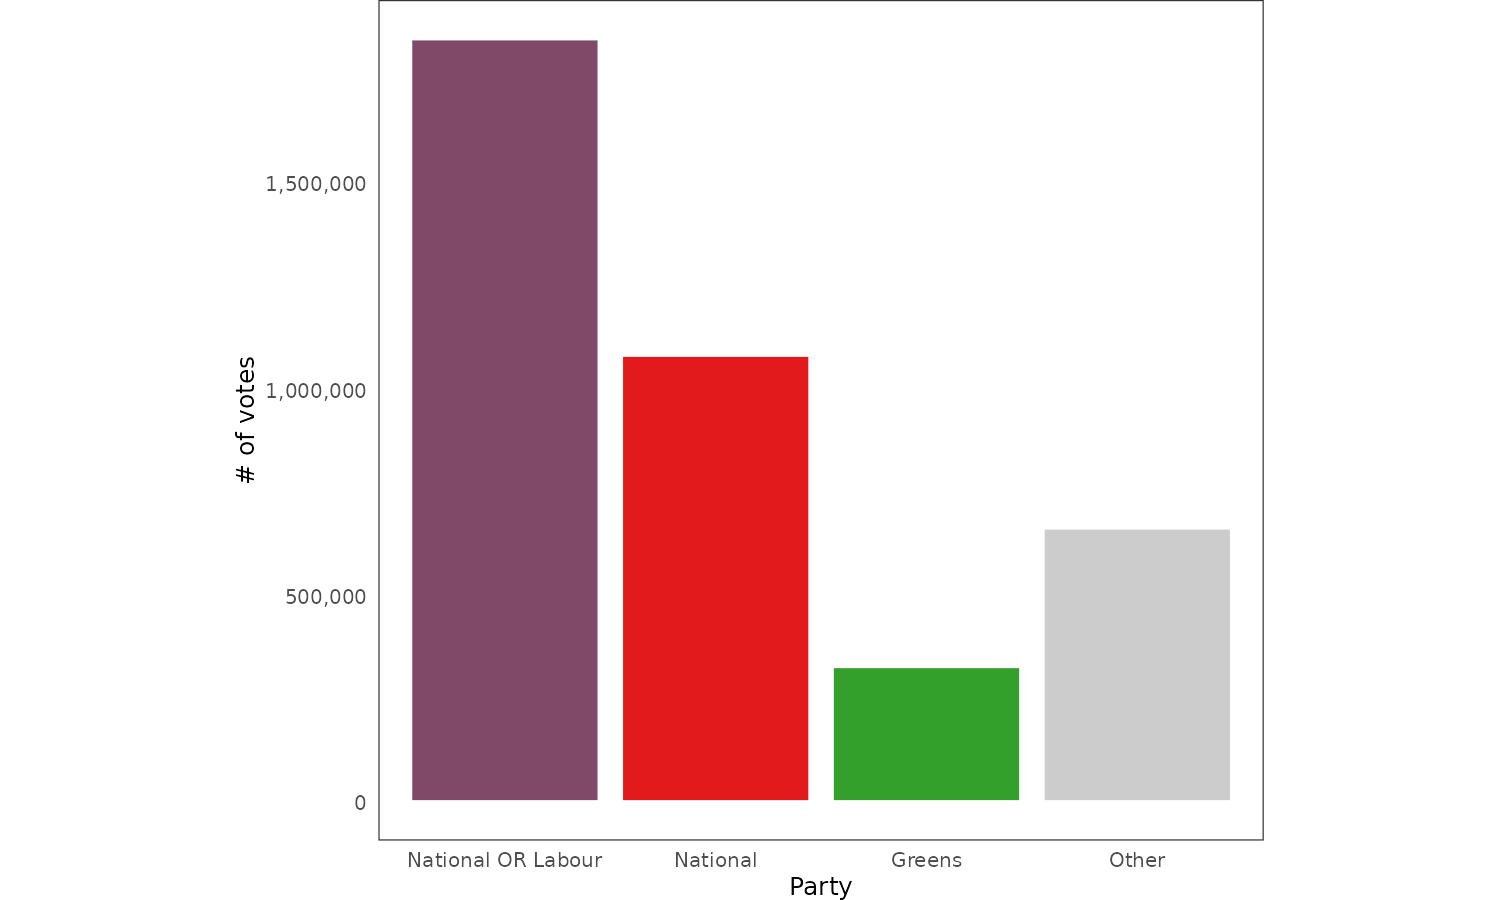
\includegraphics[width=1\linewidth,height=1\textheight]{./figures/barplot-notbijection} 

}

\caption{Barplot showing non-disjoint subsets of the data. Most of the bars show the same data as in Figure \\ref{fig:geoms-bijection}, however, the leftmost bar representing a union of National and Labour voters. The two leftmost bars are thus not disjoint. For a more realistic example, see Figure \\ref{fig:union-geoms2}.}\label{fig:union-geoms}
\end{figure}

However, this way of representing the data has several problems. First, this type of visualization is arguably not very useful for addressing our visualization goals. For example, when visualizing election data such as the one above, we typically want to compare the relative number of votes each party received. Figure \ref{fig:union-geoms} makes this comparison needlessly difficult. Specifically, since the leftmost bar represents the union of National and Labour votes, we have to perform additional mental calculation if we want to compare the number of votes received by National and Labour directly (\citeproc{ref-cleveland1985}{Cleveland 1985}). Second, we have metadata knowledge (see e.g. \citeproc{ref-wilkinson2012}{Wilkinson 2012}; \citeproc{ref-velleman1993}{Velleman and Wilkinson 1993}) about the data actually being disjoint. We know that, in the New Zealand parliament electoral system, each voter can only vote for a single party. Hence, it does not make sense to arbitrarily combine the data in this way. Finally, Figure \ref{fig:union-geoms} also needlessly duplicates information: the number of votes the National party received is counted twice, once in the leftmost bar and again in the second-from-left bar. This goes against the general principle of representing our data parsimoniously (\citeproc{ref-tufte2001}{Tufte 2001}).

Even when our goal is not to compare absolute counts, there are usually better disjoint data visualization methods available. For instance, if we were interested in visualizing the \emph{proportion} of votes that each party received, we could instead draw the following plot:

\begin{figure}

{\centering 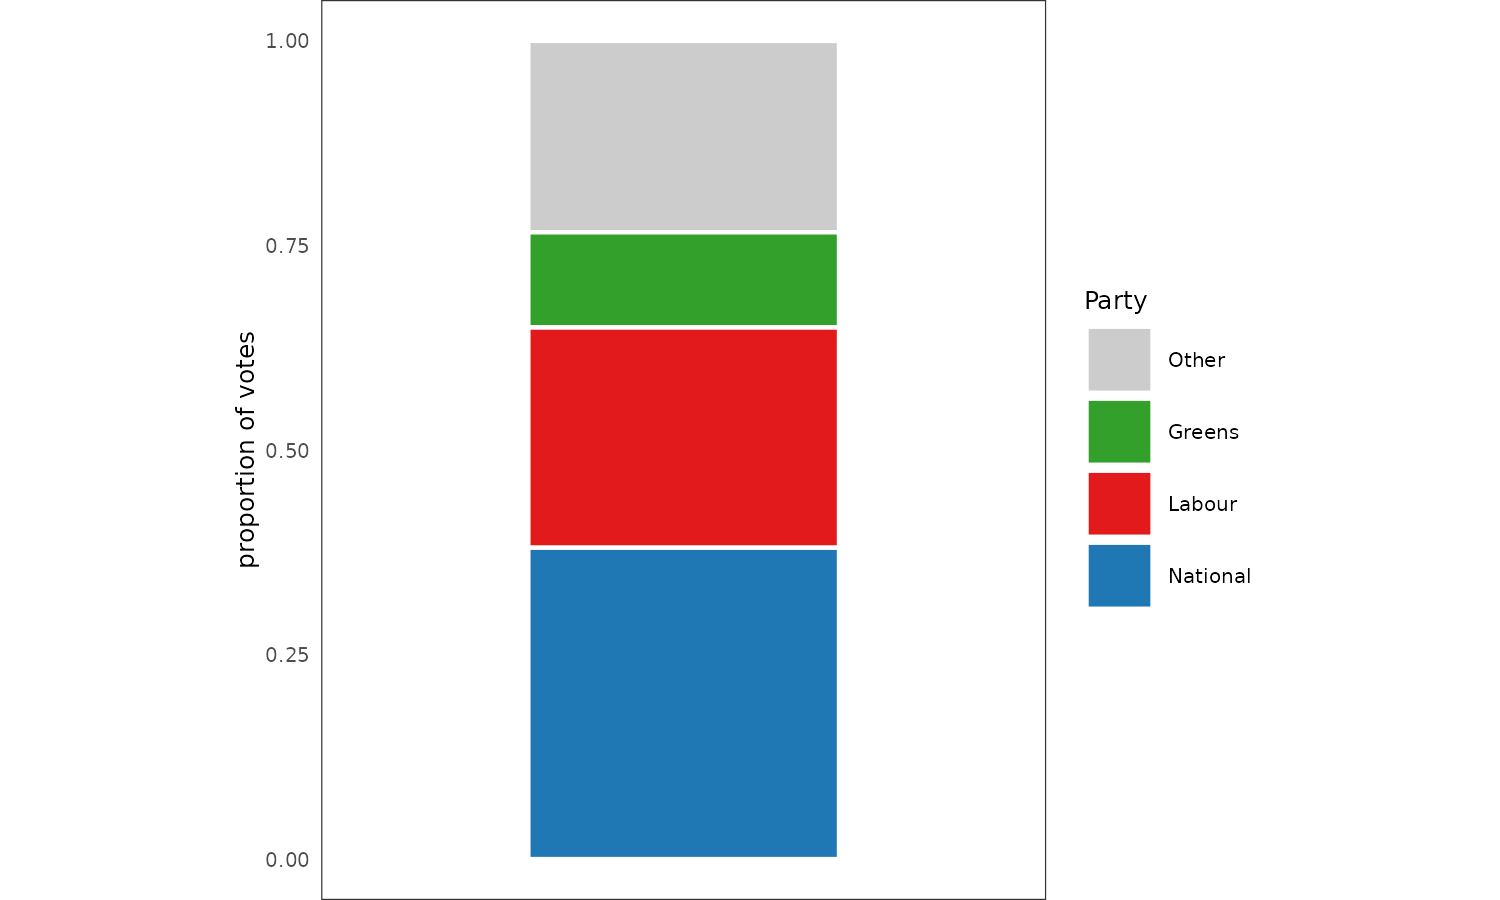
\includegraphics[width=1\linewidth,height=1\textheight]{./figures/barplot-bijection-proportions} 

}

\caption{Even when proportions are of interest, there are usually disjoint data visualization techniques available. The plot shows proportion of vote share of the top three parties in the 2023 New Zealand general election, with each bar segment again representing a unique subset of voters.}\label{fig:stacked-proportion}
\end{figure}

By stacking the bar segments on top of each other as in \ref{fig:stacked-proportion}, we can easily compare proportion of the total number of votes each party received, while retaining a disjoint representation. Each bar segment now again represents a unique subset of voters.

The example above is fairly clear-cut case of where disjoint data representation is the better choice. However, there are also more ambiguous situations, such as when multiple attributes of the data are simultaneously present or absent for each case. Take, for example, the 2020 New Zealand joint referendum on the legalization of euthanasia and cannabis. In this referendum, the two issues were included on the same ballot and voters would vote on them simultaneously. The legalization of euthanasia was accepted by the voters, with 65.1\% of votes supporting the decision, whereas the legalization of cannabis was rejected, with 50.7\% of voters rejecting the decision (\citeproc{ref-referendum2020}{Electoral Commission New Zealand 2020}).

We could visualize the referendum data in the following way:

\begin{figure}

{\centering 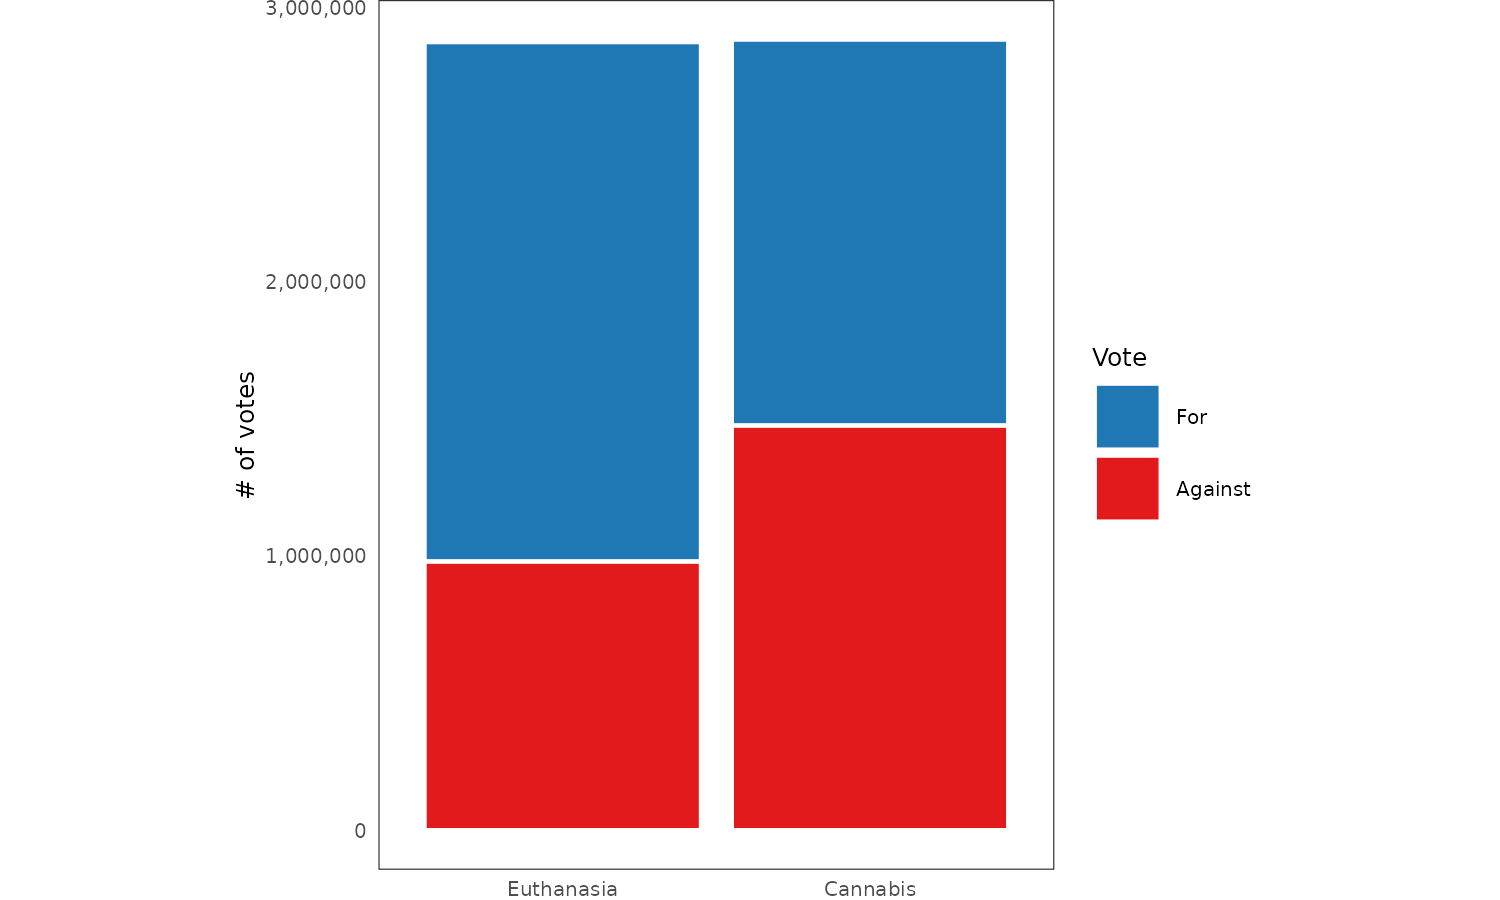
\includegraphics[width=1\linewidth,height=1\textheight]{./figures/referendum-notbijection} 

}

\caption{Barplot showing a more realistic example of non-disjoint data representation. The bars show the vote share cast by New Zealand voters in the joint 2020 referendum on euthanasia and cannabis. The two bars show (mostly) the same set of ballots, with each single ballot contributing to the height of one segment in each bar.}\label{fig:union-geoms2}
\end{figure}

In Figure \ref{fig:union-geoms2}, both bars include votes cast by the same voter (ignoring the votes where no preference was given for either issue, \citeproc{ref-referendum2020}{Electoral Commission New Zealand 2020}), making the representation non-disjoint. In
this case, the visualization works, since the underlying data is genuinely non-independent (each person cast two votes). If we had information about individual votes, it might be interesting to see how many people voted for both euthanasia and cannabis, how many voted for euthanasia but against cannabis, and so on. As was mentioned before, these types of visualizations can be useful for set-typed data (see e.g. \citeproc{ref-alsallakh2014}{Alsallakh et al. 2014}).

However, even though the data here is fundamentally non-independent, there is often a way to represent it in a disjoint way that preserves most of the desirable properties. Specifically, we can split the data and draw it as separate plots or small multiples (\citeproc{ref-tufte2001}{Tufte 2001}):

\begin{figure}

{\centering 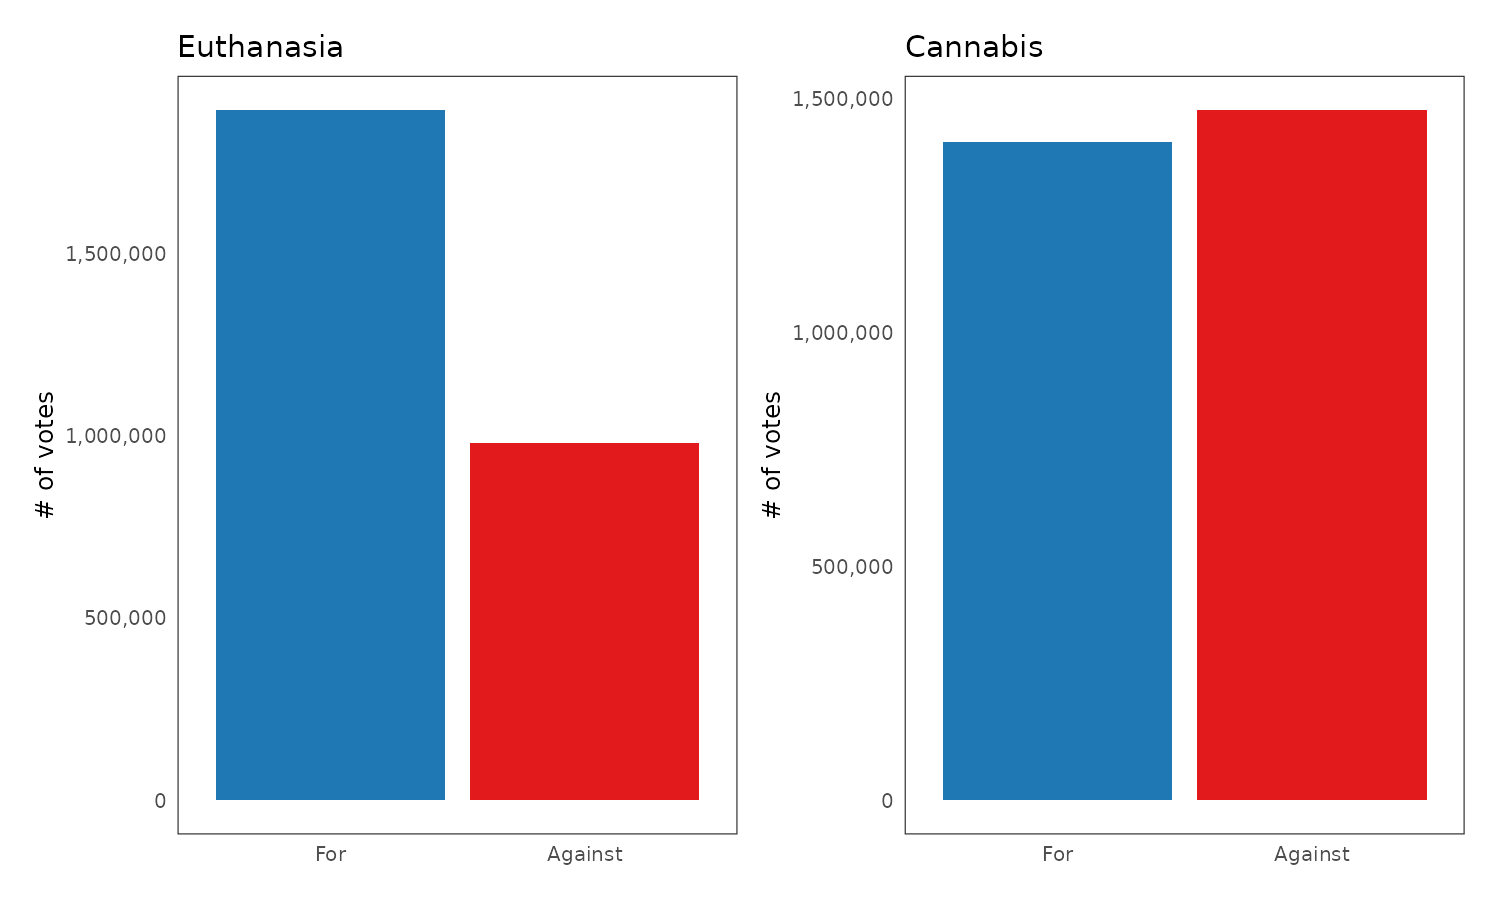
\includegraphics[width=1\linewidth,height=1\textheight]{./figures/referendum-bijection} 

}

\caption{Small multiple figure showing the non-disjoint data represented as disjoint bars. The bars again show the vote share cast by New Zealand voters in the joint 2020 referendum on euthanasia and cannabis, however, this time, each bar within one plot represents a unique subset of the cases.}\label{fig:small-multiples}
\end{figure}

Here again, in Figure \ref{fig:small-multiples}, each bar (segment) in each plot represents a disjoint subset of voters.

\subsubsection{Disjointness and interaction}\label{disjointness-and-interaction}

As I argued above, disjoint subsets offer a simpler mental model for understanding data visualizations. When each geometric object represents a unique set of data points, it becomes easier to reason about the comparisons being made. Conversely, when objects overlap or share underlying data points, additional cognitive effort is required to track the relationships between them.

Further, I argue that disjointness presents a particularly good model for interactive visualization (see also \citeproc{ref-wilhelm2008}{Wilhelm 2008}). The natural correspondence between geometric objects and subsets of the data makes certain interactions more intuitive, and conversely, overlapping subsets can produce unexpected or unintuitive behavior. For instance, when a user clicks on a bar in a linked barplot, they might reasonably expect to highlight \emph{that particular bar}, within the active plot, and the corresponding cases within all the other (passive) plots. If they see parts of other bars within the active plot get highlighted as well, they have to spend additional mental effort thinking about the relation between the objects (bars) and the subsets of the data, since this is no longer one-to-one.

Similar issue arises during querying. When a user queries an object that does not represent a disjoint subset of the data, should the returned summary statistics match the object or the (non-disjoint) subset? And how do we signal this to the user? Again, lack of disjointness introduces subtle ambiguities and complicates the interpretation of the presented information.

This does not mean that non-disjoint subsets cannot be usefuly combined with interaction, in specific contexts (see e.g. \citeproc{ref-alsallakh2014}{Alsallakh et al. 2014}; \citeproc{ref-wilhelm2008}{Wilhelm 2008}). However, I argue that, as a general model, disjointness provides a very good default. Disjoint subsets simplify our mental model, and this may be the reason why some authors discuss interactive features in the context of partitions, which are by definition disjoint (see e.g. \citeproc{ref-buja1996}{Buja, Cook, and Swayne 1996}; \citeproc{ref-keim2002}{Keim 2002}). Likewise, many common data analytic operations, such as SQL aggregation queries (\texttt{GROUP\ BY}, \citeproc{ref-hellerstein1999}{Hellerstein et al. 1999}), operate on disjoint subsets, and this may be another reason why this model is familiar.

\subsection{Plots as partitions}\label{plots-as-partitions}

In the two preceding sections, I have argued that it is generally desirable for plots in our (interactive) data visualization system to have two fundamental features:

\begin{itemize}
\tightlist
\item
  Completeness: They should show the full data
\item
  Distinctness: Geometric objects should represent distinct subsets of data points
\end{itemize}

These two features actually map onto two fundamental mathematical properties: \hyperref[Functions]{surjectivity} and \hyperref[Partitions]{disjointness}. In turn, these two properties define a well-known mathematical structure: a \hyperref[Partitions]{partition}. Therefore, partitions offer a compelling model for structuring our plots. I propose the following definition of a \emph{regular plot}:

\begin{definition}[Regular plot]
Regular plot is a plot where the geometric objects within one layer represent a partition of the data, such that there is a bijection between these objects and (possibly aggregated) subsets of the original data.
\end{definition}

Note that this definition still allows for plots where geometric objects in different layers represent overlapping data subsets, such as boxplots with overlaid points, or scatterplots with a smooth fit.

I propose regular plots as a fundamental building block of our interactive data visualization system. By building our interactive figures out of regular plots (as small multiples, \citeproc{ref-tufte2001}{Tufte 2001}), we can ensure that the resulting visualization will be easily interpretable, even when combined with interactive features such as linking and querying.

\subsubsection{Bijection on cases vs.~bijection on subsets}\label{bijection-on-cases-vs.-bijection-on-subsets}

Although I have not been able to find references conceptualizing plots as partitions in the same general way as I do here, some data visualization researchers have used the language of bijections when discussing graphics. For example, Dastani (\citeproc{ref-dastani2002}{2002}) discusses plots as bijections (homomorphisms) between data tables and visual attribute tables. Similarly, Ziemkiewicz and Kosara (\citeproc{ref-ziemkiewicz2009}{2009}), and Vickers, Faith, and Rossiter (\citeproc{ref-vickers2012}{2012}) argue that, in order to be visually unambiguous, plots should represent bijections of the underlying data. Essentially, these researchers argue that plots should represent bijective mappings of the data tables, such that each object represents one row of the data.

However, this ``one-row-one-object'' model sidesteps the issue of aggregation (see also Section \ref{aggregation}). It operates on the assumption that the data is pre-aggregated, such that, for instance, when we draw a barplot or a histogram, we start with a table that has one row per bar. This is rarely the case in practice. Most visualization systems incorporate aggregation as an explicit component of the data visualization pipeline (see e.g. \citeproc{ref-chi2000}{Chi 2000}; \citeproc{ref-wickham2016}{Wickham 2016}; \citeproc{ref-satyanarayan2015}{Satyanarayan et al. 2015}, \citeproc{ref-satyanarayan2016}{2016}; \citeproc{ref-wu2024}{Wu and Chang 2024}). Howeever, acknowledging aggregation presents a problem for the one-row-one-object model, since aggregation is, by definition, not injective. Once we aggregate multiple data points into a summary or a set of summaries, we cannot recover the original cases (see also \citeproc{ref-wu2024}{Wu and Chang 2024}). Thus, the model proposed by authors such as Dastani (\citeproc{ref-dastani2002}{2002}), Ziemkiewicz and Kosara (\citeproc{ref-ziemkiewicz2009}{2009}), and Vickers, Faith, and Rossiter (\citeproc{ref-vickers2012}{2012}) would exclude many common aggregation-based types of plots, such as barplots and histograms. Ziemkiewicz and Kosara (\citeproc{ref-ziemkiewicz2009}{2009}) indeed do acknowledge that this is a problem, and admit that, at times, aggregation can be an acceptable trade-off, despite the inherent information loss.

However, if we instead model plots as bijection between \emph{parts of data} and the geometric objects, rather than between individual \emph{data points} and geometric objects, aggregation ceases to be a problem. Even after we aggregate a multiple-row subset of the data into a single row summary, this bijection is preserved. Thus, aggregation can be considered a part of the bijection. For instance, if we split our data into ten tables and aggregate each table, we are still left with ten tables of one row each that we can map bijectively to geometric objects.

\subsubsection{Products of partitions}\label{products-of-partitions}

Many types of plots involve data that has partitioned or split across multiple dimensions. This is especially true in interactive data visualization, where features such as linking automatically induce another level of partitioning (\citeproc{ref-wilhelm2008}{Wilhelm 2008}). This necessitates a general mechanism for combining partitions into products.

The concept of ``product of partitions'' may be best illustrated with code examples. Suppose we want to draw the following barplot:

\begin{center}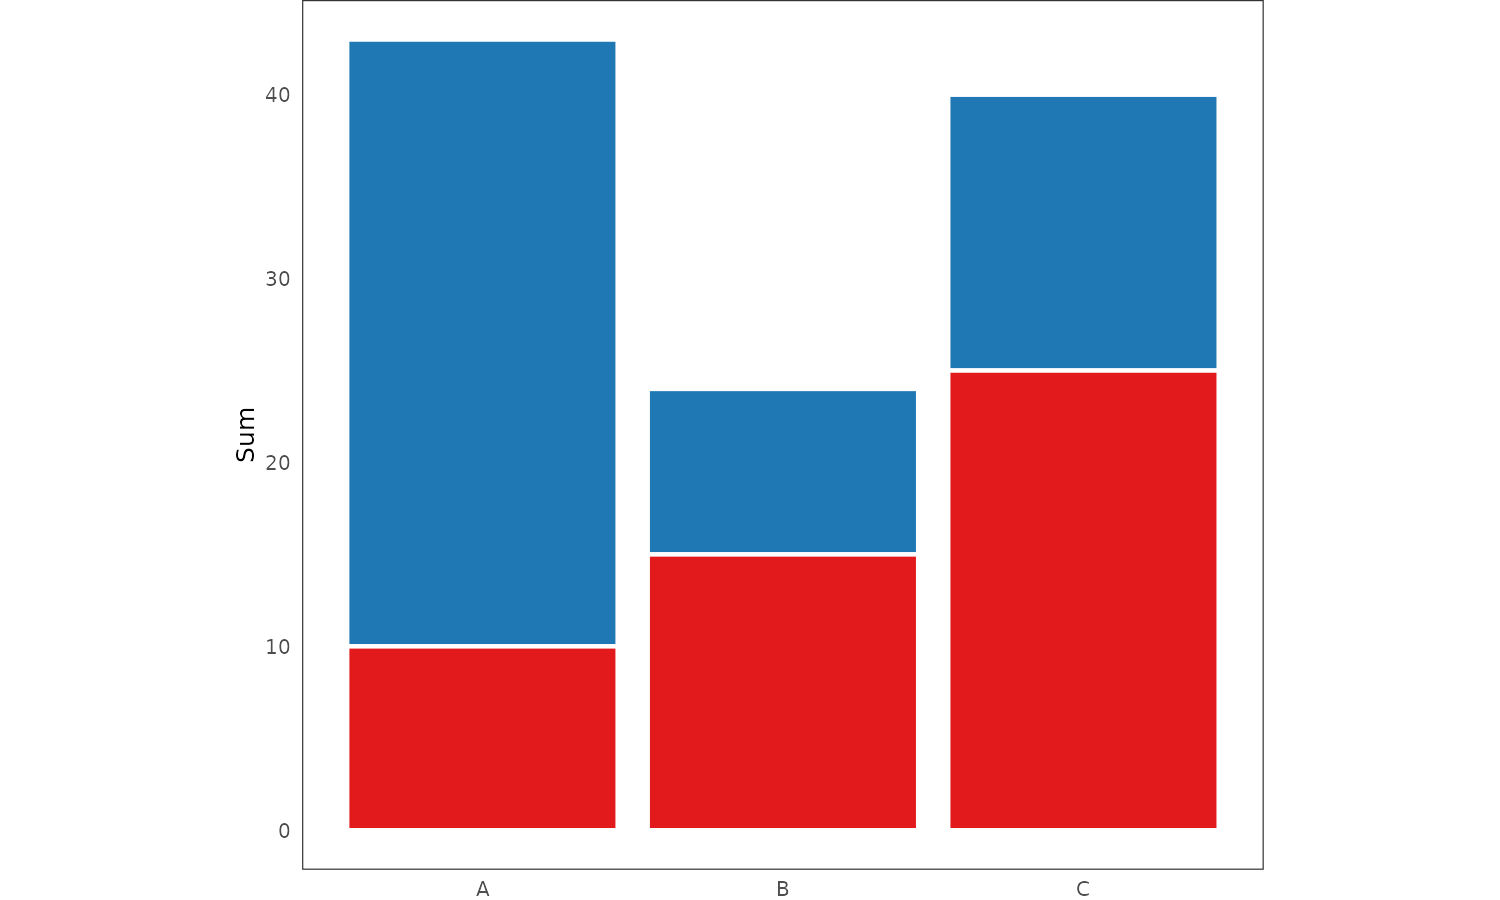
\includegraphics[width=1\linewidth,height=1\textheight]{./figures/barplot-partitions-products} \end{center}

We start with the following data, which includes a categorical variable (\texttt{group}, plotted along the x-axis), a variable representing selection status (\texttt{selection}, used to colour the bar segments), and a continuous variable that we want to summarize (\texttt{value}):

\begin{table}
\centering
\begin{tabular}{l|l|l|r}
\hline
  & group & selection & value\\
\hline
1 & A & 1 & 12\\
\hline
2 & A & 1 & 21\\
\hline
3 & A & 2 & 10\\
\hline
4 & B & 1 & 9\\
\hline
5 & B & 2 & 15\\
\hline
6 & C & 1 & 15\\
\hline
7 & C & 2 & 12\\
\hline
8 & C & 2 & 13\\
\hline
\end{tabular}
\end{table}

To draw individual bar segments, we need to sum \texttt{value} across the subsets cases corresponding to each segment. To do this, we first need to split our data into multiple subsets corresponding to the partition formed by taking the product of \texttt{group} and \texttt{selection} variables.

In R, the general data structure for representing partitions is the \texttt{factor} S3 class. In a \texttt{factor}, all elements of a vector are assigned a label, such that each label represent one disjoint part of the data. Unfortunately, there is no built-in function for creating a Cartesian product of two factors. However, we can easily emulate it using \texttt{paste} function to combine factor levels as strings element-wise:

\begin{Shaded}
\begin{Highlighting}[]
\NormalTok{product\_factor }\OtherTok{\textless{}{-}} \FunctionTok{paste}\NormalTok{(df}\SpecialCharTok{$}\NormalTok{group, df}\SpecialCharTok{$}\NormalTok{selection)}
\NormalTok{split\_dfs }\OtherTok{\textless{}{-}} \FunctionTok{split}\NormalTok{(df, product\_factor)}
\FunctionTok{render\_tables}\NormalTok{(split\_dfs)}
\end{Highlighting}
\end{Shaded}

\begin{table}
\begin{table}
\centering
\begin{tabular}{l|l|r}
\hline
group & selection & value\\
\hline
A & 1 & 12\\
\hline
A & 1 & 21\\
\hline
\end{tabular}
\end{table}\begin{table}
\centering
\begin{tabular}{l|l|l|r}
\hline
  & group & selection & value\\
\hline
3 & A & 2 & 10\\
\hline
\end{tabular}
\end{table}
\end{table}\begin{table}
\begin{table}
\centering
\begin{tabular}{l|l|l|r}
\hline
  & group & selection & value\\
\hline
4 & B & 1 & 9\\
\hline
\end{tabular}
\end{table}\begin{table}
\centering
\begin{tabular}{l|l|l|r}
\hline
  & group & selection & value\\
\hline
5 & B & 2 & 15\\
\hline
\end{tabular}
\end{table}
\end{table}\begin{table}
\begin{table}
\centering
\begin{tabular}{l|l|l|r}
\hline
  & group & selection & value\\
\hline
6 & C & 1 & 15\\
\hline
\end{tabular}
\end{table}\begin{table}
\centering
\begin{tabular}{l|l|l|r}
\hline
  & group & selection & value\\
\hline
7 & C & 2 & 12\\
\hline
8 & C & 2 & 13\\
\hline
\end{tabular}
\end{table}
\end{table}

We can then summarize each small data set by summing \texttt{value}:

\begin{Shaded}
\begin{Highlighting}[]
\NormalTok{summarized\_dfs }\OtherTok{\textless{}{-}} \FunctionTok{lapply}\NormalTok{(split\_dfs, }\ControlFlowTok{function}\NormalTok{(x) \{}
  \FunctionTok{aggregate}\NormalTok{(value }\SpecialCharTok{\textasciitilde{}}\NormalTok{ ., }\AttributeTok{data =}\NormalTok{ x, sum)}
\NormalTok{\})}

\FunctionTok{render\_tables}\NormalTok{(summarized\_dfs)}
\end{Highlighting}
\end{Shaded}

\begin{table}
\begin{table}
\centering
\begin{tabular}{l|l|r}
\hline
group & selection & value\\
\hline
A & 1 & 33\\
\hline
\end{tabular}
\end{table}\begin{table}
\centering
\begin{tabular}{l|l|r}
\hline
group & selection & value\\
\hline
A & 2 & 10\\
\hline
\end{tabular}
\end{table}
\end{table}\begin{table}
\begin{table}
\centering
\begin{tabular}{l|l|r}
\hline
group & selection & value\\
\hline
B & 1 & 9\\
\hline
\end{tabular}
\end{table}\begin{table}
\centering
\begin{tabular}{l|l|r}
\hline
group & selection & value\\
\hline
B & 2 & 15\\
\hline
\end{tabular}
\end{table}
\end{table}\begin{table}
\begin{table}
\centering
\begin{tabular}{l|l|r}
\hline
group & selection & value\\
\hline
C & 1 & 15\\
\hline
\end{tabular}
\end{table}\begin{table}
\centering
\begin{tabular}{l|l|r}
\hline
group & selection & value\\
\hline
C & 2 & 25\\
\hline
\end{tabular}
\end{table}
\end{table}

Finally, to ``stack'' the segments on top of each other, we need to combine the summaries back together, within the levels of \texttt{group} variable. We can do this by grouping the data sets by the \texttt{group} variable and taking their cumulative sum:

\begin{Shaded}
\begin{Highlighting}[]
\NormalTok{grouped\_dfs }\OtherTok{\textless{}{-}} \FunctionTok{split}\NormalTok{(summarized\_dfs, }\FunctionTok{sapply}\NormalTok{(summarized\_dfs, }\ControlFlowTok{function}\NormalTok{(x) x}\SpecialCharTok{$}\NormalTok{group))}
\NormalTok{stacked\_dfs }\OtherTok{\textless{}{-}} \FunctionTok{lapply}\NormalTok{(grouped\_dfs, }\ControlFlowTok{function}\NormalTok{(x) \{}
\NormalTok{  x }\OtherTok{\textless{}{-}} \FunctionTok{do.call}\NormalTok{(rbind, x)}
\NormalTok{  x}\SpecialCharTok{$}\NormalTok{value }\OtherTok{\textless{}{-}} \FunctionTok{cumsum}\NormalTok{(x}\SpecialCharTok{$}\NormalTok{value)}
  \FunctionTok{rownames}\NormalTok{(x) }\OtherTok{\textless{}{-}} \ConstantTok{NULL} \CommentTok{\# Remove rownames for nicer formatting}
\NormalTok{  x}
\NormalTok{\})}

\FunctionTok{render\_tables}\NormalTok{(stacked\_dfs)}
\end{Highlighting}
\end{Shaded}

\begin{table}
\begin{table}
\centering
\begin{tabular}{l|l|r}
\hline
group & selection & value\\
\hline
A & 1 & 33\\
\hline
A & 2 & 43\\
\hline
\end{tabular}
\end{table}\begin{table}
\centering
\begin{tabular}{l|l|r}
\hline
group & selection & value\\
\hline
B & 1 & 9\\
\hline
B & 2 & 24\\
\hline
\end{tabular}
\end{table}
\end{table}\begin{table}
\centering
\begin{tabular}{l|l|r}
\hline
group & selection & value\\
\hline
C & 1 & 15\\
\hline
C & 2 & 40\\
\hline
\end{tabular}
\end{table}

Now, we can combine these tables into one \texttt{data.frame} and render:

\begin{Shaded}
\begin{Highlighting}[]
\NormalTok{combined\_df }\OtherTok{\textless{}{-}} \FunctionTok{do.call}\NormalTok{(rbind, stacked\_dfs)}
\CommentTok{\# Need to reverse factor and row order for ggplot2 to layer segments correctly}
\NormalTok{combined\_df}\SpecialCharTok{$}\NormalTok{selection }\OtherTok{\textless{}{-}} \FunctionTok{factor}\NormalTok{(combined\_df}\SpecialCharTok{$}\NormalTok{selection, }\AttributeTok{levels =} \FunctionTok{c}\NormalTok{(}\DecValTok{2}\NormalTok{, }\DecValTok{1}\NormalTok{))}
\NormalTok{combined\_df }\OtherTok{\textless{}{-}}\NormalTok{ combined\_df[}\DecValTok{6}\SpecialCharTok{:}\DecValTok{1}\NormalTok{, ] }

\FunctionTok{ggplot}\NormalTok{(combined\_df, }\FunctionTok{aes}\NormalTok{(}\AttributeTok{x =}\NormalTok{ group, }\AttributeTok{y =}\NormalTok{ value, }\AttributeTok{fill =}\NormalTok{ selection)) }\SpecialCharTok{+}
  \FunctionTok{geom\_col}\NormalTok{(}\AttributeTok{position =} \FunctionTok{position\_identity}\NormalTok{())}
\end{Highlighting}
\end{Shaded}

\begin{center}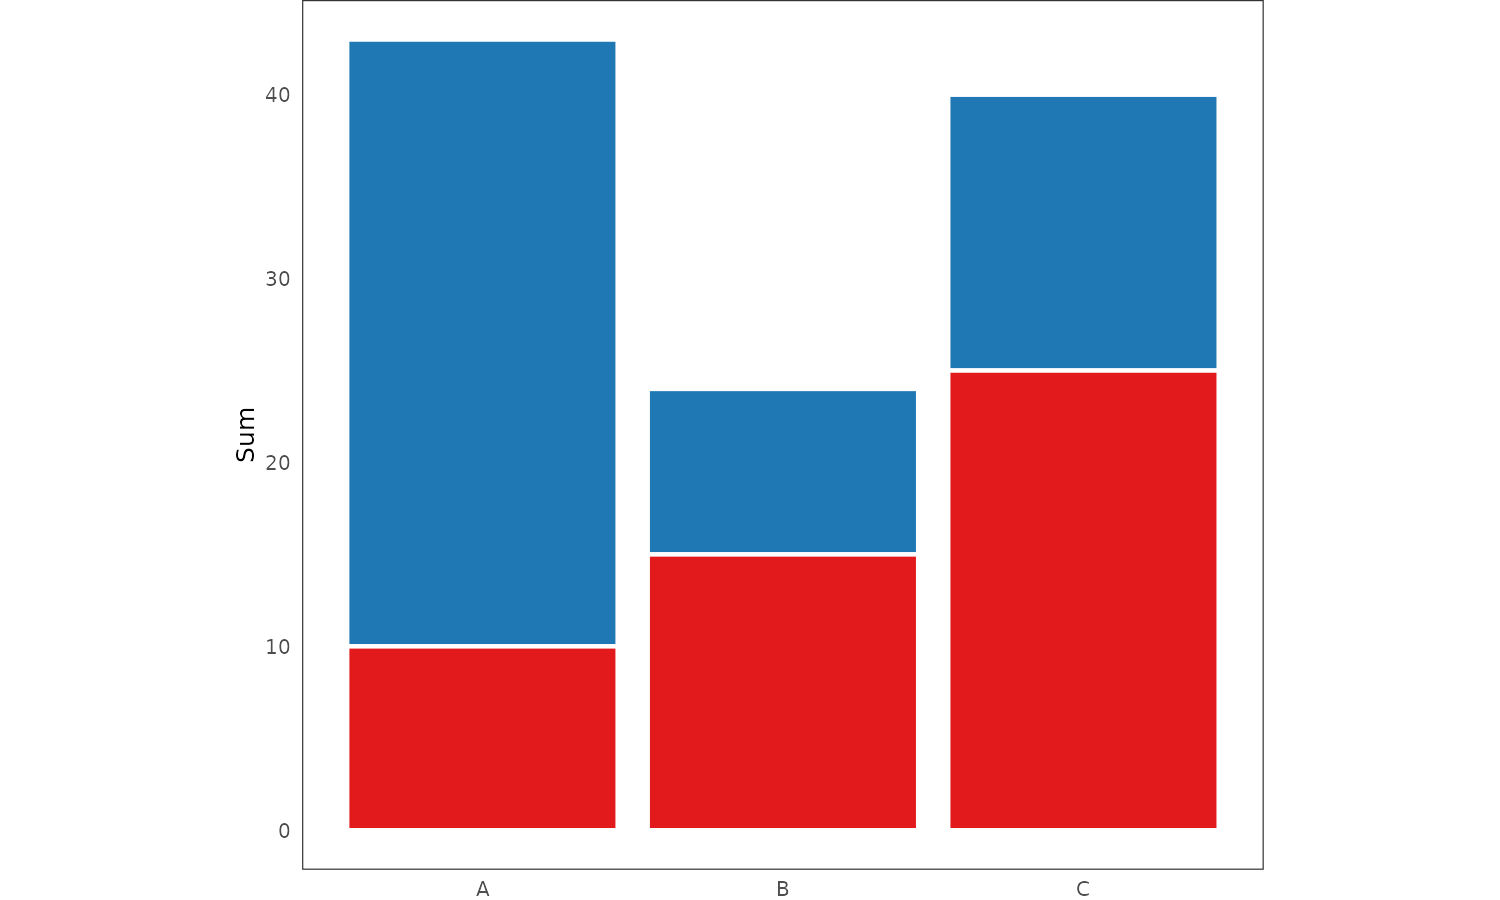
\includegraphics[width=1\linewidth,height=1\textheight]{./figures/barplot-partitions-products} \end{center}

What we have just shown is an example of a simple split-apply-combine pipeline (\citeproc{ref-wickham2011}{Wickham 2011}). This type of a pipeline is necessary in most types of plots and data visualization systems. For instance, the following \texttt{ggplot2} call produces a similar data visualization pipeline like the one we described above:

\begin{Shaded}
\begin{Highlighting}[]
\FunctionTok{ggplot}\NormalTok{(data, }\FunctionTok{aes}\NormalTok{(x, y, }\AttributeTok{fill =}\NormalTok{ fill)) }\SpecialCharTok{+}
  \FunctionTok{geom\_bar}\NormalTok{(}\AttributeTok{stat =} \StringTok{"summary"}\NormalTok{, }\AttributeTok{fun =} \StringTok{"sum"}\NormalTok{)}
\end{Highlighting}
\end{Shaded}

To be more explicit, in the \texttt{ggplot2} call above, we specify that we want to partition the data set by the Cartesian product of the \texttt{x}, \texttt{y}, and \texttt{fill} variables. See the following comment from the \href{https://github.com/tidyverse/ggplot2/blob/f46805349d6ca8ca7a99f8966cfa0f29279c2f6c/R/grouping.R\#L7}{\texttt{ggplot2} documentation} (\citeproc{ref-wickham2016}{Wickham 2016}):

\begin{Shaded}
\begin{Highlighting}[]
\CommentTok{\# If the \textasciigrave{}group\textasciigrave{} variable is not present, then a new group}
\CommentTok{\# variable is generated from the interaction of all discrete (factor or}
\CommentTok{\# character) vectors, excluding \textasciigrave{}label\textasciigrave{}.}
\end{Highlighting}
\end{Shaded}

We then compute whatever summary we want (\texttt{sum}). Finally, when a \texttt{fill} or \texttt{col} aesthetic is used with \texttt{geom\_bar}, \texttt{ggplot2} also automatically stack the bars on top of each other by summing their heights. Similar strategy is employed for many other types of stacked plots, including pie charts, histograms, or density plots (\citeproc{ref-wickham2016}{Wickham 2016}).

\subsubsection{Limits of flat product partitions}\label{limits-of-flat-product-partitions}

For many common plot types, a single ``flat'' product of all factors/partitions works reasonably well. However, for other types of plots, this simple model is not enough. Specifically, certain types of plots exhibit hierarchical relationships between the partitions which cannot be represented under this flat model (see also \citeproc{ref-slingsby2009}{Slingsby, Dykes, and Wood 2009}; \citeproc{ref-wu2022}{Wu 2022}).

To give a concrete example, let's turn back to the barplot from the section above (\ref{plots-as-partitions}). To draw the barplot, we first split our data into smaller tables, summarized each table by summing the values, stacked the summaries by taking their cumulative sum, and finally used the resulting data frame to render bar segments. This gave us a stacked barplot, which is a good visualization for comparing absolute counts across categories.

However, what if, instead of comparing absolute counts, we wanted to compare proportions? It turns out there is another type of visualization, called the spineplot, which can be used to represent the same underlying data as a barplot, however, is much better suited for comparing proportions:

\begin{figure}

{\centering 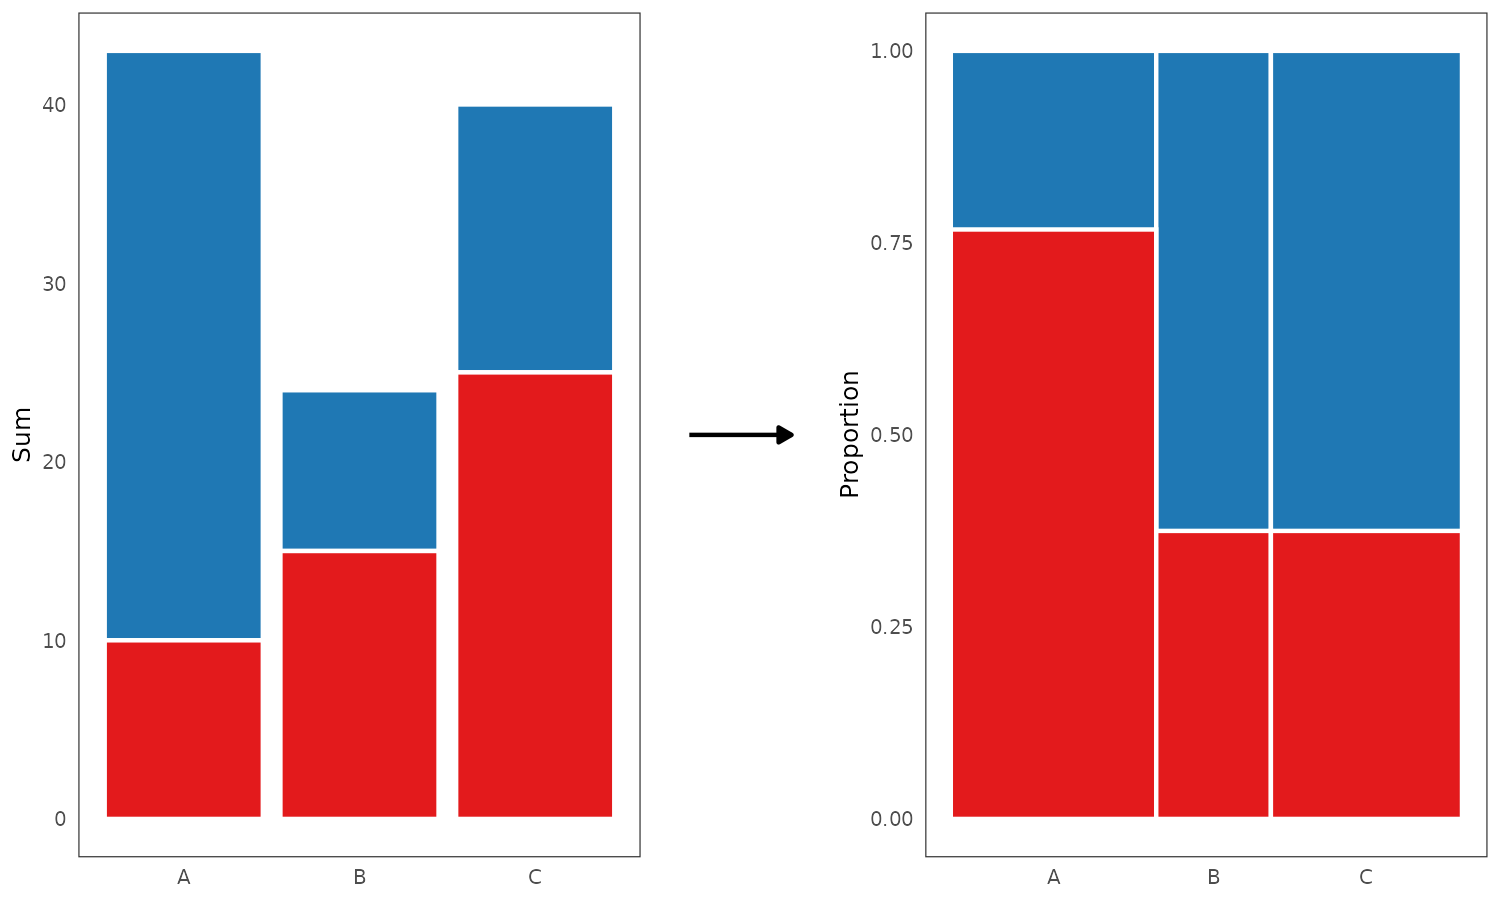
\includegraphics[width=1\linewidth,height=1\textheight]{./figures/barplot-spineplot} 

}

\caption{The same underlying data represented as a barplot (left) and a spineplot (right).}\label{fig:barplot-spineplot}
\end{figure}

Like barplots, spineplots represent some summary statistic (usually counts), aggregated within the levels of a product of two categorical variables. However, unlike barplots, spineplots map the underlying statistics to both the y-axis position (height) and the bar width. Furthermore, the y-axis position is normalized, such that the heights of the different segments within the same category add up to one. This normalization makes it possible to compare the relative frequencies within categories directly (notice how the right panel in Figure \ref{fig:barplot-spineplot} makes it obvious that the proportion of red cases within the B and C categories is the same). Thus, like the barplot, the spineplot is a valuable tool for visualizing categorical data, especially when we can use interactive features to switch from one type of representation to the other.

Although barplot and spineplot represent the same underlying data, turning one into the other is not always easy. Specifically, while many grammar-based visualization systems offer a simple declarative syntax for defining barplots, they lack such simple syntax for spineplots. For instance, to draw a spineplot in \texttt{ggplot2}, we first need to do a substantial amount of data wrangling (creating the plot in the right panel of Figure \ref{fig:barplot-spineplot} took over 10 lines of code, using standard \texttt{dplyr} syntax). This same hierarchical dependence applies to other ``normalized'' types of plots, such as spinograms, as well as innately hierarchical displays such as treemaps and mosaic plots {[}see e.g. Theus (\citeproc{ref-theus2002}{2002}); slingsby2009{]}.

\subsection{Partitions, hierarchy, and preorders}\label{hierarchy}

Why are spineplots so tricky? The reason is that they force us to confront the hierarchical nature of (interactive) graphics (\citeproc{ref-mcdonald1990}{McDonald, Stuetzle, and Buja 1990}; \citeproc{ref-keller2024}{Keller, Manz, and Gehlenborg 2024}). Specifically, while in a barplot, we can get by with a single flat partition of the data, in a spineplot, the data is summarized and stacked \emph{along and across} different levels of aggregation (\citeproc{ref-wu2024}{Wu and Chang 2024}):

\begin{itemize}
\tightlist
\item
  Along the x-axis, we stack the summaries \emph{across the levels of the top-level factor/category}
\item
  Along the y-axis, we stack the summaries \emph{across the levels of a product of two factors} and normalize them by the values \emph{within the levels of the top-level factor}.
\end{itemize}

For example, assume we have a data set with two categorical variables, with \(j\) and \(k\) levels respectively. If we want to render a spineplot using these two variables, it is not enough to simply split our data into \(j \cdot k\) tables. Instead, we need to partition our data twice: first, split it into \(j\) tables, and second, split it into \(j \cdot k\) tables. We also need to keep track of which of the \(j\) tables on the first level of partitioning \emph{corresponds} to each of the \(j \cdot k\) smaller tables. This automatically induces a hierarchical relationship, where the resulting data subsets form a graph - specifically, a tree - see Figure \ref{fig:spineplot-tree}:

\begin{figure}

{\centering 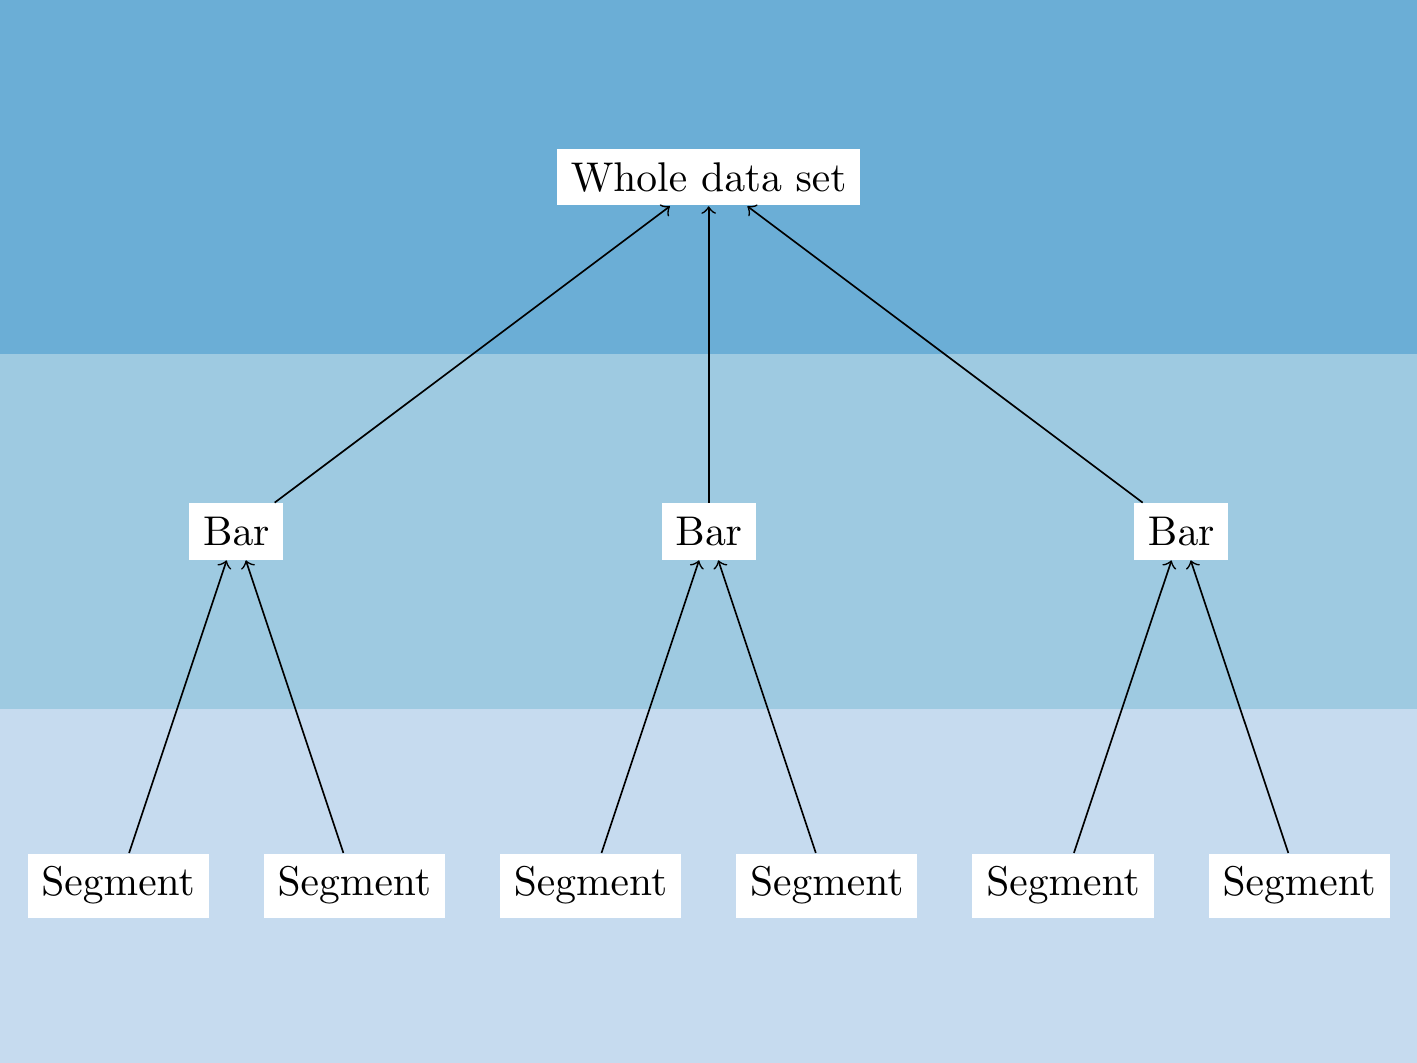
\includegraphics[width=1\linewidth,height=1\textheight]{./figures/spineplot-tree} 

}

\caption{A diagram of the hierarchical relationship between the subsets of the data represented by a spineplot/barplot. The whole data set is partitioned into bars, which are in turn partitioned into bar segments.}\label{fig:spineplot-tree}
\end{figure}

In \ref{fig:spineplot-tree}, each vertical level represents a data partition, and arrows indicate relationships between data subsets, such that a bar subset is composed of segment subsets, and the whole data set is in turn composed of bar subsets. This same tree can be used to represent both barplots and spineplots. For a stacked barplot, this tree structure can be implicit, since we can work with the lowest level of the partitioning only (the segments; ignoring details such as maintaining correct stacking order). However, for spineplots, this hierarchical structure is essential. In spineplots, we apply transformations \emph{across} the levels of the hierarchy: we need to normalize the statistics corresponding to each segment by the values within the parent bar. This is only possible if each segment can reference its parent bar in some way.

Thus, to be able to model a broad class of plots, we need a way to encode a hierarchical partitioning of our data. Furthermore, for reasons that will become clear later, it may be beneficial to introduce a more formal, mathematical framework for thinking about this hierarchy. A simple algebraic structure for encoding such class of hierarchies is a preorder.

\subsubsection{Plots as preorders}\label{plots-as-preorders}

A \hyperref[preorders]{preorder} is a binary relation on a set \(S\), generally denoted by \(\leq\), that is both reflexive and transitive. In simpler terms, given a preordered set \(S\), any two elements \(a, b \in S\) either relate (\(a \leq b\), meaning \(a\) is ``less than'' \(b\)), or they do not relate at all. Further, the relation obeys some common sense properties: every element relates to itself (reflexivity), and if \(a\) relates to \(b\) and \(b\) relates to \(c\), then \(a\) relates to \(c\) as well (transitivity).

We can turn our hierarchy of data subsets in Figure \ref{fig:spineplot-tree} into a preorder very easily, by simply being more explicit about the relations, see Figure \ref{fig:barplot-preorder}. Specifically, define set \(S\) as the set of data subsets \(D\), with the individual subsets indexed by identity such that e.g.~\(D_D\) corresponds to the whole data set, \(D_{B_1}, \ldots D_{B_n}\) correspond to bar subsets, and \(D_{S_1}, \ldots D_{S_k}\) correspond to segment subsets. Further, define the binary relation \(\leq\) as the set inclusion relation \(\subseteq\).

\begin{figure}

{\centering 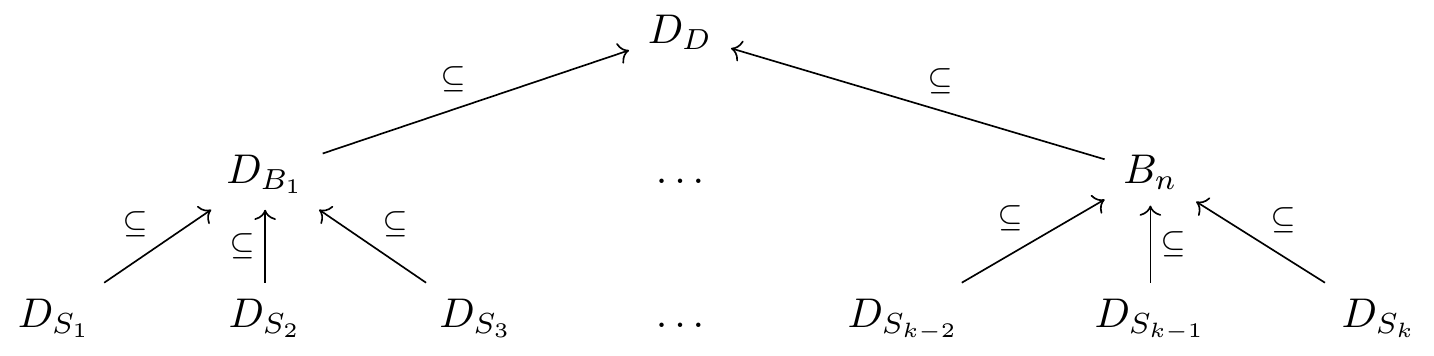
\includegraphics[width=1\linewidth,height=1\textheight]{./figures/barplot-preorder} 

}

\caption{A diagram of a barplot or spinogram, represented as a preorder ordered by set inclusion. $D_D$ represents the whole data set, $D_{B_i}$ represent bar subsets, and $D_{S_j}$ represent individual bar segment subsets. Arrows indicate set inclusion.}\label{fig:barplot-preorder}
\end{figure}

Then, we see that the two properties of preorders do indeed hold: every data subset is included in itself (reflexivity), and if a segment subset is a part of a bar subset, and bar subset is a part of the whole data set, then the segment subset is, clearly, a part of the whole data set as well (transitivity).

While set inclusion (\(\subseteq\)) is a perfectly valid way to describe the relation between data subsets, a slightly different perspective using set union \((\cup)\) will be more beneficial later. Specifically, instead of stating that a segment subset is included in a bar subset, we can express the relation by stating that a segment subset can be combined with another set to form the bar subset:

\begin{figure}

{\centering 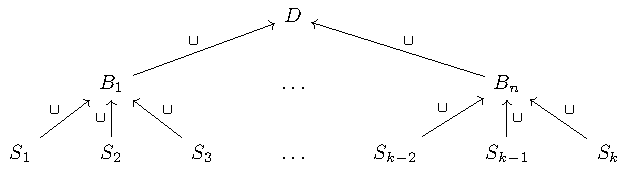
\includegraphics[width=1\linewidth,height=1\textheight]{./figures/barplot-preorder2} 

}

\caption{A more precise version of the diagram of a barplot/spinogram, with the relation identified as set union with the sibling subsets.}\label{fig:barplot-preorder2}
\end{figure}

This definition is still fairly vague, however, it will be made more precise in Section \ref(preorders-categories). To summarize the key points, our data subset hierarchy can be described as a preorder, where the ordering is defined by a kind of set union operation. This is really the same idea as Figure \ref{fig:spineplot-tree}, we are simply being more explicit about our data assumptions. The real utility of this approach will be revealed later, in Section \ref{aggregation}. However, for now, it may be useful to revise our definition of a regular plot:

\begin{definition}[Regular plot 2]
Regular plot is a plot where the geometric objects within one layer represent a preorder of data subsets ordered by set inclusion/union (such that there is a bijection between these objects and the data subsets, and the subsets on the same order level represent a partition of the data).
\end{definition}

\subsubsection{The graph behind the graph}\label{the-graph-behind-the-graph}

To summarize the main point of this entire section, \emph{graphs are graphs}. As a bit of a playful side-note, this view is not shared by everyone. Particularly, the poster of the following meme shared on the Mathematical Mathematics Memes Facebook group (\citeproc{ref-mathematicalmathematics2024}{Martínez 2024}) might not agree:

\begin{figure}

{\centering 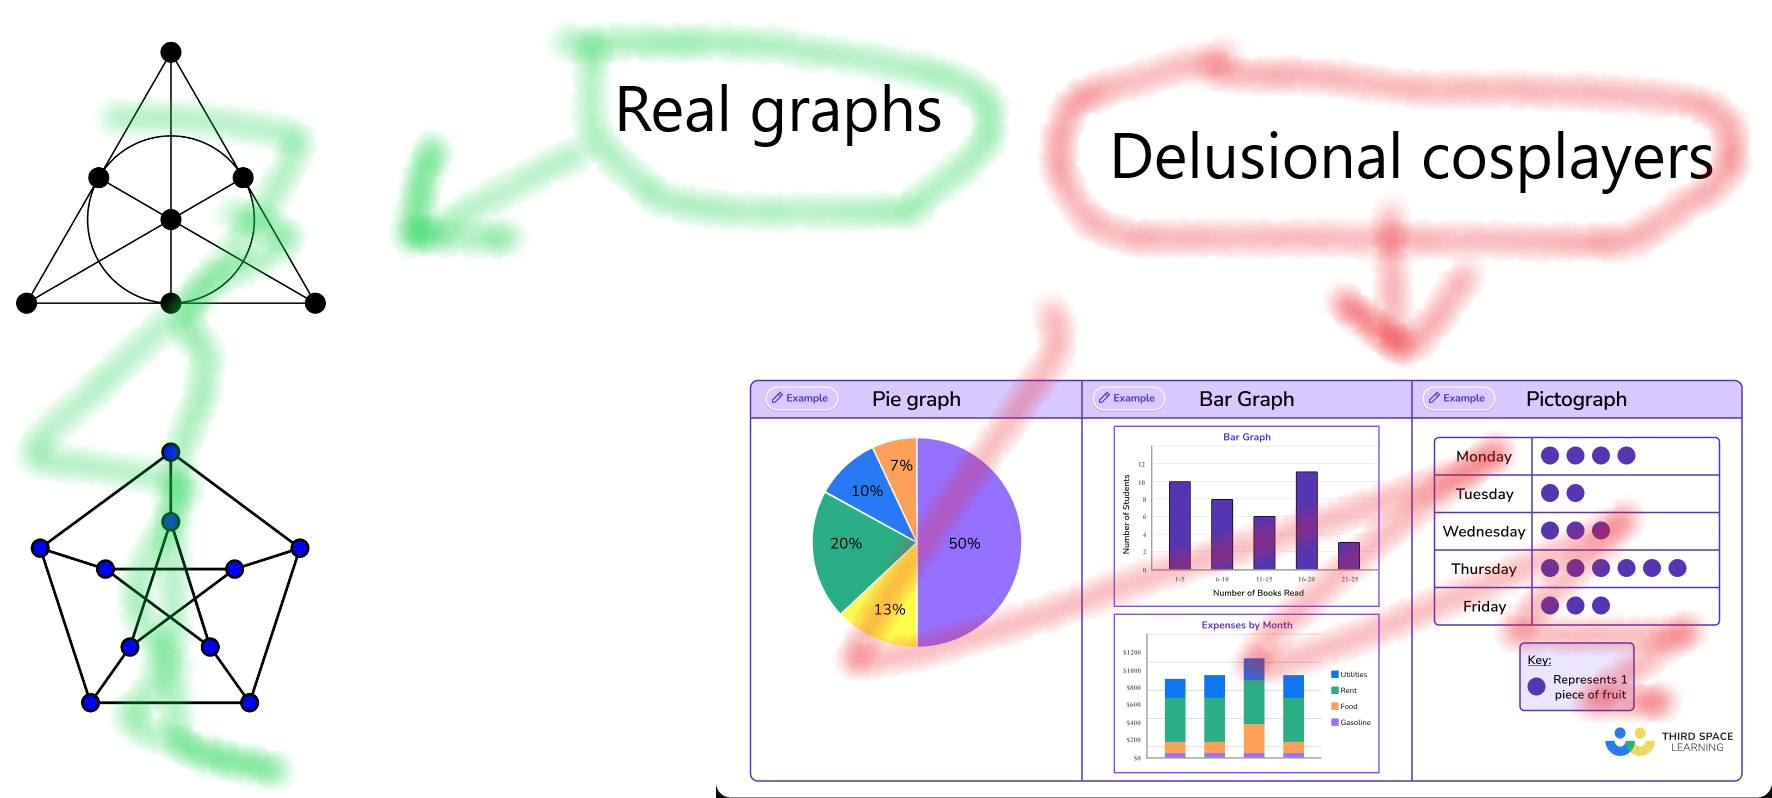
\includegraphics[width=0.75\linewidth,height=1\textheight,style="border:1px solid black;"]{./figures/graphs-cosplayers} 

}

\caption{A joke image shared in the Mathematical Mathematics Memes Facebook group on the 28th of March, 2024 [@mathematicalmathematics2024].}\label{fig:meme}
\end{figure}

I hope I have made a reasonably strong case here that many data visualization types are not ``delusional cosplayers''. By organizing our data into a preorder, we induce a graph-like, part-whole relationship on the subsets. Thus, graphs really are graphs.

However, organizing our data into a preorder introduces a new kind of challenge: preserving the inherent structure. Preorders, as algebraic objects, have structure encoded in their order relations. Intuitively, it would be wrong to disregard this structure in the subsequent steps of the data visualization pipeline. For instance, imagine taking a barplot, dividing the bars into segments, and then stacking half of the segments while placing the other half side-by-side. Clearly, something would be wrong with this approach. Visualization methods should respect the inherent hierarchy within our data.

However, what does it \emph{really} mean to respect the structure of our data? This question will be explored in detail in the following section, which deals with the next step of the data visualization pipeline: aggregation.

\section{Aggregation}\label{aggregation}

\begin{quote}
``This system cannot produce a meaningless graphic, however. This is a strong claim, vulnerable to a single counter-example. It is a claim based on the formal rules of the system, however, not on the evaluation of specific graphics it may produce.''

``Some of the combinations of graphs and statistical methods may be degenerate or bizarre, but there is no moral reason to restrict them.''

Wilkinson (\citeproc{ref-wilkinson2012}{2012}), The Grammar of Graphics, pp.~15 and 112.
\end{quote}

The second step of any data visualization pipeline is aggregation. Specifically, after we split our data into a hierarchy of parts (a preorder), we need to summarize each part via a set of summary statistics. Further, as I have hinted at in the previous section, these summaries should respect the hierarchical nature of the data. Thus, while the computing summaries may seem like a fairly straightforward step in the visualization pipeline, there is more complexity here than meets the eye. This will be the main subject of the present section.

\subsection{The relationship between graphics and statistics}\label{the-relationship-between-graphics-and-statistics}

A key issue in data visualization, which is also the central theme of the present thesis, concerns the relationship between graphics and statistics. Specifically, when we summarize our data and then render these summaries as geometric objects, an important question arises: can we pair arbitrary statistics and geometric objects? Or are there constraints which limit which statistics and geometric objects can be effectively combined, particularly when interaction is involved?

\subsubsection{Independence: The grammar-based model}\label{independence-the-grammar-based-model}

The approach of treating graphics and statistics as independent entities is highly appealing. Indeed, it is the cornerstone of the immensely popular ``grammar-based'' model of visualization, introduced by Wilkinson in his seminal work The Grammar of Graphics (\citeproc{ref-wilkinson2012}{2012}). Under this model, visualizations are constructed out of independent, modular components, such as geometric objects, statistics, scales, and coordinate systems. See the following quote by Wilkinson (\citeproc{ref-wilkinson2012}{2012, 14--15}):

\begin{quote}
``We have tried to avoid adding functions, graphs, or operators that do not work independently across the system. There are doubtless many statistical graphics the system in this book cannot completely specify. We can add many different graphs, transformations, types of axes, annotations, etc., but there are two limitations we will always face with a formal system.
\end{quote}

The grammar-based model offers many advantages, including simplicity and expressive power. This has contributed to its widespread adoption and implementation in many data visualization systems (see e.g. \citeproc{ref-mcnutt2022}{McNutt 2022}; \citeproc{ref-kim2022}{Kim et al. 2022}; \citeproc{ref-vanderplas2020}{Vanderplas, Cook, and Hofmann 2020}; \citeproc{ref-wickham2010}{Wickham 2010}; \citeproc{ref-satyanarayan2014}{Satyanarayan, Wongsuphasawat, and Heer 2014}; \citeproc{ref-satyanarayan2016}{Satyanarayan et al. 2016}). The canonical example is the famous \texttt{ggplot2} package (\citeproc{ref-wickham2010}{Wickham 2010}). In \texttt{ggplot2}, plots are built out of components such as geometric objects (called \texttt{geoms}), statistical summaries (\texttt{stats}), and scales. These components can be flexibly combined, allowing the user to express a wide range of graphics using a small set of primitives. The expressive power of \texttt{ggplot2} has made it one of the most popular R packages of all time.\footnote{Being the top most downloaded CRAN package as of 4th of December 2024, Data Science Meta (\citeproc{ref-rmeta2024}{2024})}.

However, despite its advantages, the grammar-based model has one fundamental flaw: graphics and statistics are not truly independent (see also \citeproc{ref-wu2024}{Wu and Chang 2024}). Instead, the visual representation of data must be congruent with its mathematical properties. This constraint, while present even in static visualizations, becomes especially critical in interactive contexts. Let's illustrate this point with an example of real-world data.

\subsubsection{Motivating example: Limits of independence}\label{stacking-not-graphical}

For this example, I will use famous data set from a study on the effect of smoking on child lung capacity (\citeproc{ref-tager1979}{Tager et al. 1979}; \citeproc{ref-kahn2005}{Kahn 2005}). In the study, the researchers measured children's forced expiratory volume (FEV), and recorded it alongside age, height, sex, and smoking status.

A rather surprising feature of this data set is that, at a glance, the children who smoked actually had greater lung volume than non-smokers. In \texttt{ggplot2}, we can easily create a boxplot showing the relationship between smoking status and FEV using the following short code snippet:

\begin{Shaded}
\begin{Highlighting}[]
\NormalTok{fev }\OtherTok{\textless{}{-}} \FunctionTok{read.csv}\NormalTok{(}\StringTok{"./data/fev.csv"}\NormalTok{)}

\FunctionTok{library}\NormalTok{(ggplot2)}

\FunctionTok{ggplot}\NormalTok{(fev, }\FunctionTok{aes}\NormalTok{(smoke, fev, }\AttributeTok{fill =}\NormalTok{ smoke)) }\SpecialCharTok{+}
  \FunctionTok{geom\_boxplot}\NormalTok{()}
\CommentTok{\# There is actually a bit more code involved in producing the plot below,}
\CommentTok{\# but it all just has to do with design/aesthetic flair}
\end{Highlighting}
\end{Shaded}

\begin{center}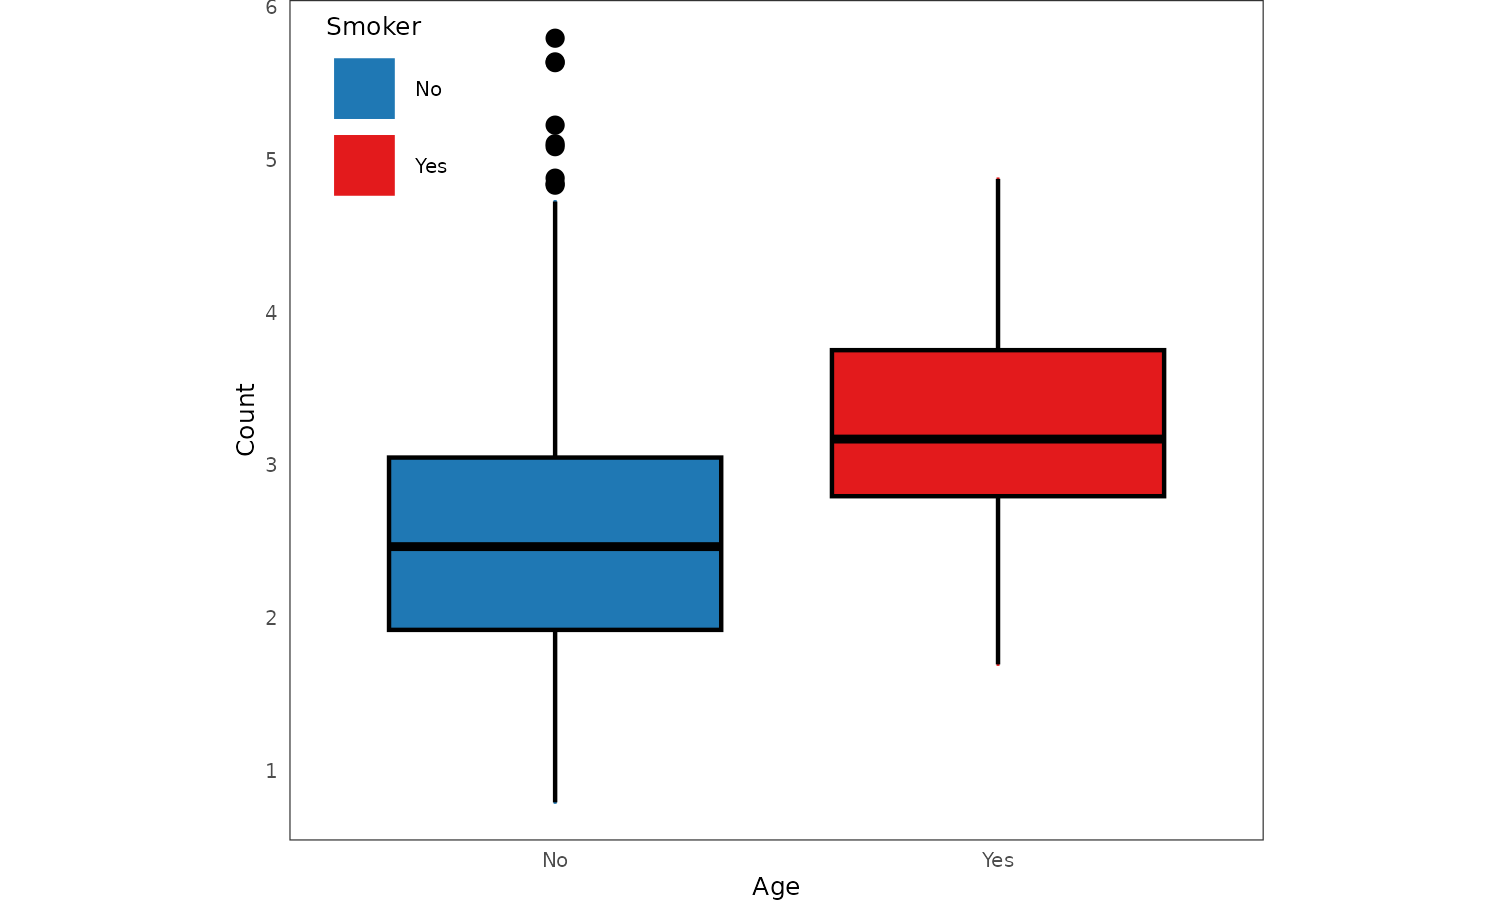
\includegraphics[width=1\linewidth,height=1\textheight]{./figures/grammar-boxplot} \end{center}

Before we start extolling the benefits of smoking for juvenile lung health, it may be a good idea to first look at some confounding variables. Lung volume develops with age, and the researchers had collected data from children ages three and up. Clearly, there were not going to be many smokers among three-year olds, so we should make sure age is not a confounder.

We can verify that there indeed is a strong relationship between age and FEV like so:

\begin{Shaded}
\begin{Highlighting}[]
\FunctionTok{ggplot}\NormalTok{(fev, }\FunctionTok{aes}\NormalTok{(age, fev, }\AttributeTok{fill =}\NormalTok{ smoke)) }\SpecialCharTok{+}
  \FunctionTok{geom\_point}\NormalTok{()}
\end{Highlighting}
\end{Shaded}

\begin{center}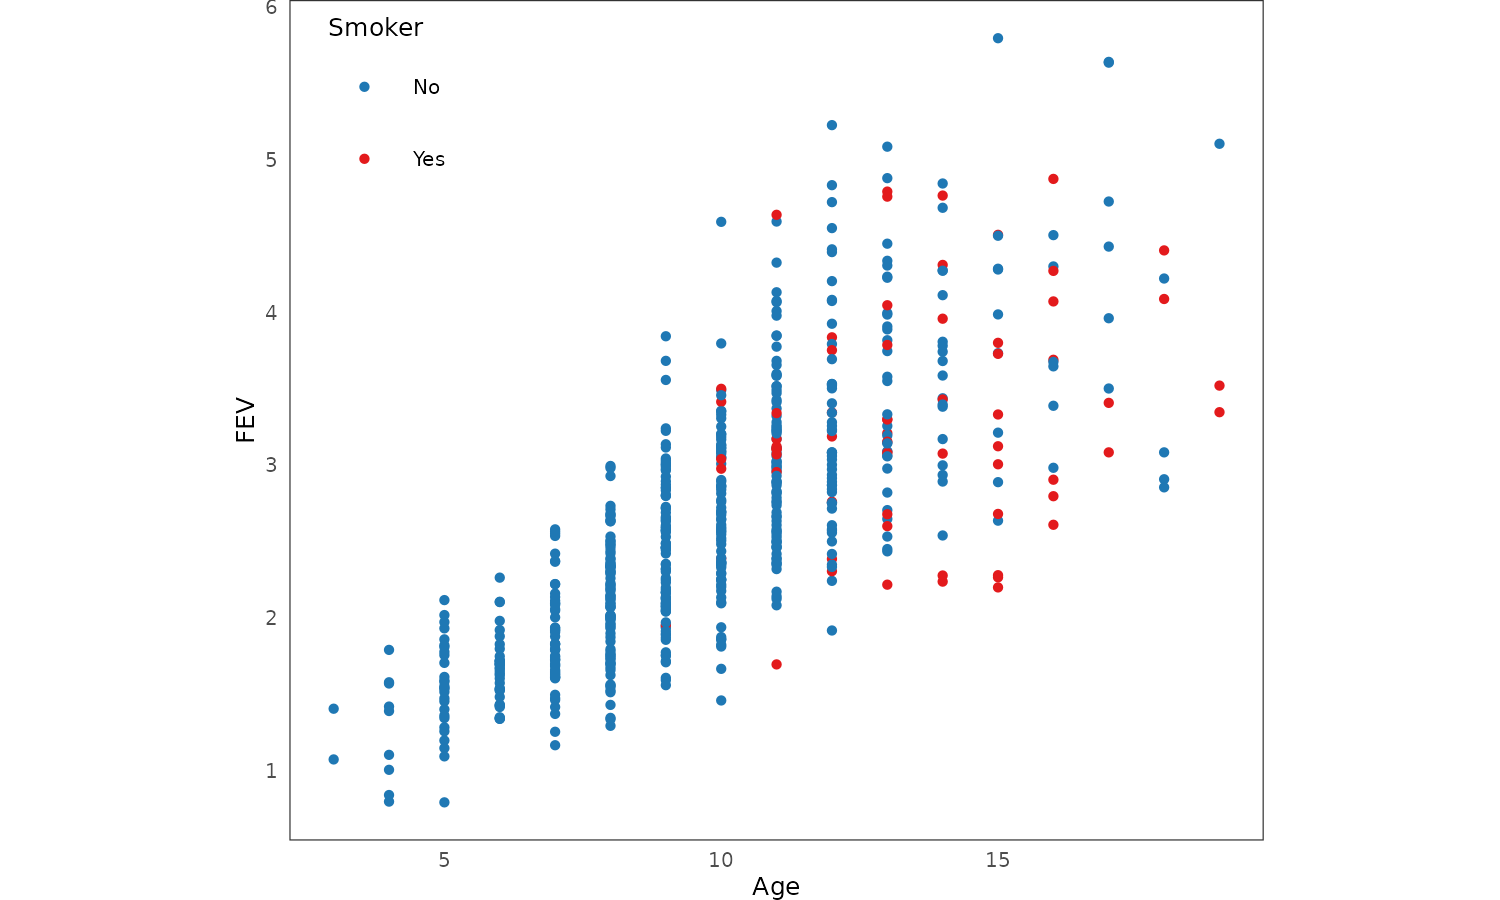
\includegraphics[width=1\linewidth,height=1\textheight]{./figures/grammar-scatterplot} \end{center}

From the plot above, we can see that age and FEV correlate strongly, and also that the smokers tend to be quite a bit older than the non-smokers. To visualize the distribution of smokers and non-smokers across age a bit more clearly, we can draw an ordinary stacked barplot:

\begin{Shaded}
\begin{Highlighting}[]
\FunctionTok{ggplot}\NormalTok{(fev, }\FunctionTok{aes}\NormalTok{(age, fev, }\AttributeTok{fill =}\NormalTok{ smoke)) }\SpecialCharTok{+}
  \FunctionTok{geom\_bar}\NormalTok{()}
\end{Highlighting}
\end{Shaded}

\begin{figure}

{\centering 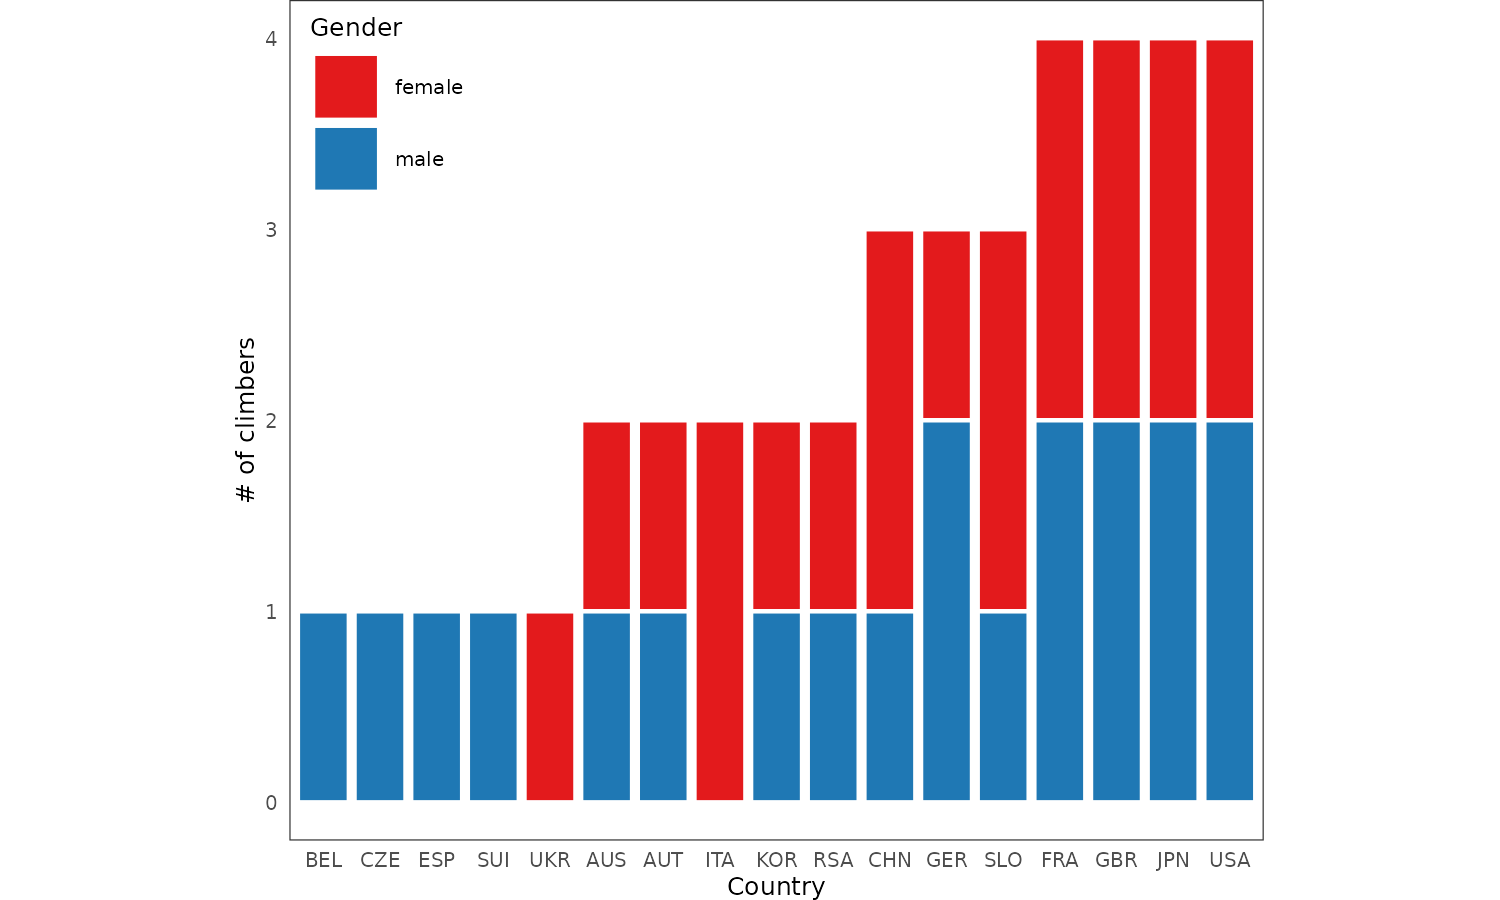
\includegraphics[width=1\linewidth,height=1\textheight]{./figures/grammar-barplot-counts} 

}

\caption{The number of participants by age and smoking status. Notice that the bar segments 'stack', such that the height of the whole bar accurately represents the combined number of smokers and non-smokers.}\label{fig:grammar-barplot-counts}
\end{figure}

The plot above clearly shows that there were more smokers than non-smokers, and that smokers tended to be on average older. This provides a support for our confounding hypothesis.

Now, what if we wanted to compare FEV across the different ages? A data visualization novice might do something like below, and draw a stacked barplot of the average FEV in each age group:

\begin{Shaded}
\begin{Highlighting}[]
\FunctionTok{ggplot}\NormalTok{(fev, }\FunctionTok{aes}\NormalTok{(age, fev, }\AttributeTok{fill =}\NormalTok{ smoke)) }\SpecialCharTok{+}
  \FunctionTok{geom\_bar}\NormalTok{(}\AttributeTok{stat =} \StringTok{"summary"}\NormalTok{, }\AttributeTok{fun =} \StringTok{"mean"}\NormalTok{)}
\end{Highlighting}
\end{Shaded}

\begin{figure}

{\centering 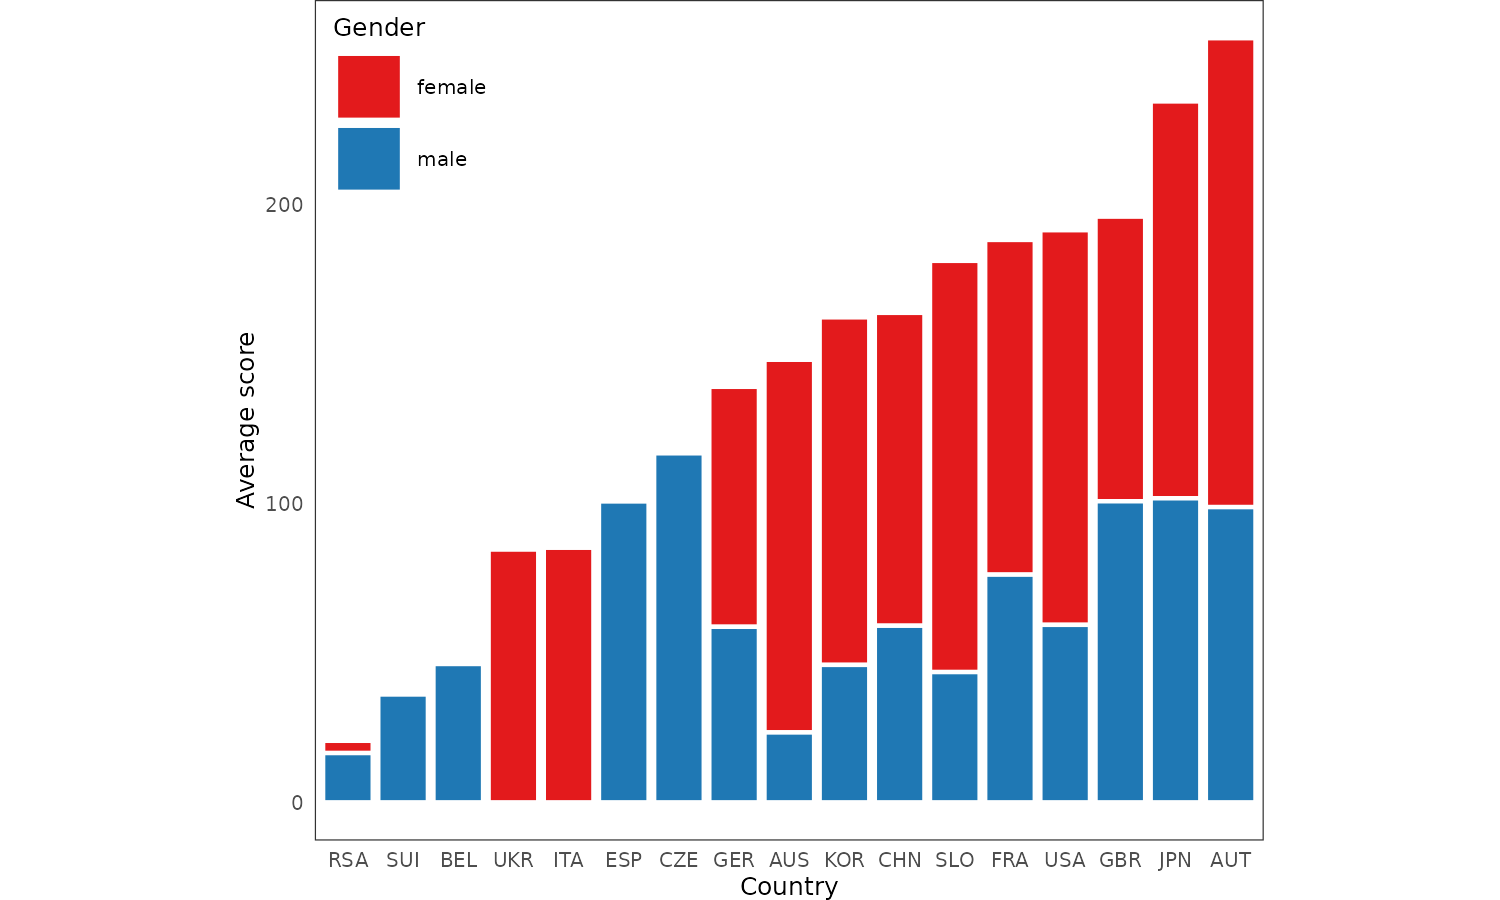
\includegraphics[width=1\linewidth,height=1\textheight]{./figures/grammar-barplot-means} 

}

\caption{A fundamentally flawed visualization of the average FEV by age and smoking status. Notice that the total height of the stacked bars is meaningless: it represents the sum of grouped averages, which is not a valid summary of the combined smoker and non-smoker data.}\label{fig:grammar-barplot-means}
\end{figure}

At a glance, the plot in \ref{fig:grammar-barplot-means} looks fine. However, what do the heights of the stacked bars actually represent? Each coloured bar segment represents a mean of the \texttt{fev} variable, grouped by the levels defined by the product of the \texttt{age} and \texttt{smoke} variables. By stacking the bars on top of each other, we are essentially summing up the average FEV of smokers and non-smokers, within the given age category.

\subsubsection{Some statistics are stackable but others are not}\label{some-statistics-are-stackable-but-others-are-not}

The visualization in \ref{fig:grammar-barplot-means} is problematic because the bar heights lack a meaningful statistical interpretation. The sum of group means is not something that most consumers of visualizations would know how to interpret or care about. In the previous example, in Figure \ref{fig:grammar-barplot-counts}, the heights of the stacked bars represented valid overall counts - the number of smokers and non-smokers within a given age category combined. In Figure \ref{fig:grammar-barplot-means}, this is no longer the case - the sum of the group means is different from the mean of the combined cases, and so may be the mean of the group means.

In \texttt{ggplot2}, stacking is implemented as a purely graphical operation. That is, within the context of the visualization system, stacking operates on geometric objects (rectangles), irrespective of the underlying summary statistics. However, as we can see from the example above, this can cause problems - \emph{what} we stack matters. Indeed, many data visualization researchers have explicitly warned about this problem:

\begin{quote}
``Stacking is useful when the sum of the amounts represented by the individual stacked bars is in itself a meaningful amount'' (\citeproc{ref-wilke2019}{Wilke 2019, 52}).
\end{quote}

\begin{quote}
``Because this gives the visual impression of one element that is the sum of several others, it is very important that if the element's size is used to display a statistic, then that statistic must be summable. Stacking bars that represent counts, sums, or percentages are fine, but a stacked bar chart where bars show average values is generally meaningless.'' (\citeproc{ref-wills2011}{G. Wills 2011, 112}).
\end{quote}

\begin{quote}
``{[}\ldots{]} We do this to ensure that aggregate statistics are always computed over the input data, and so users do not inadvertantly compute e.g., averages of averages, which can easily lead to misinterpretation.'' (\citeproc{ref-wu2022}{Wu 2022})
\end{quote}

Based on the quotes above, one might get the impression that we can only ever ``stack'' or ``highlight'' sums and counts, to get a valid combined summary statistics. However, take a look at the following plot:

\begin{Shaded}
\begin{Highlighting}[]
\CommentTok{\# Code is not included because this plot cannot be recreated }
\CommentTok{\# with a simple ggplot2 call (without data wrangling)}
\end{Highlighting}
\end{Shaded}

\begin{figure}

{\centering 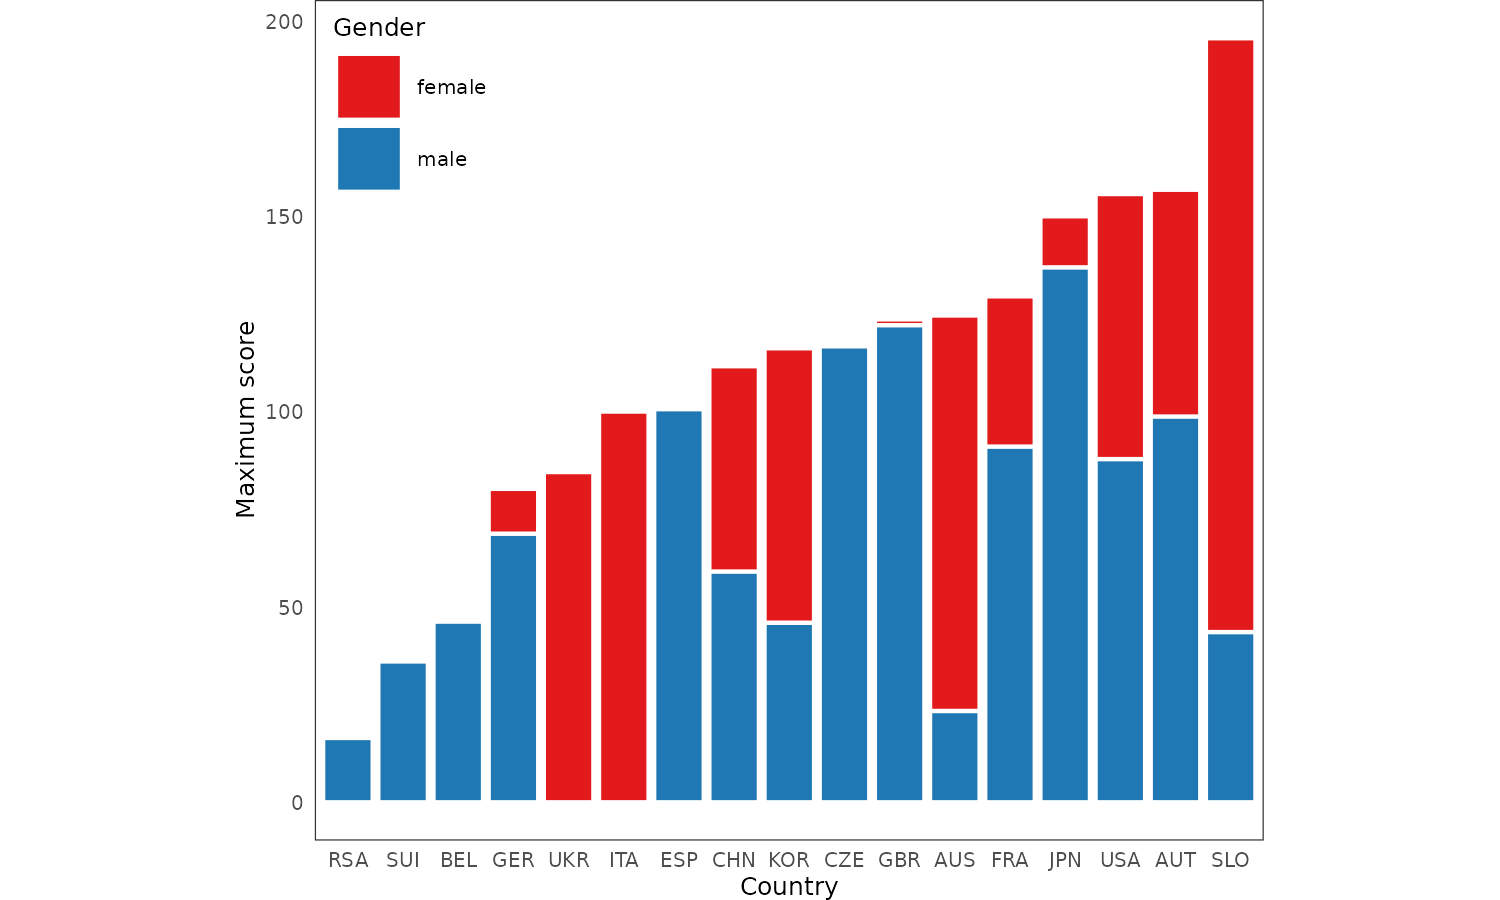
\includegraphics[width=1\linewidth,height=1\textheight]{./figures/grammar-barplot-maximums} 

}

\caption{The maximum of maxima is a valid maximum of all cases.}\label{fig:grammar-barplot-maximums}
\end{figure}

Here, in Figure \ref{fig:grammar-barplot-maximums}, we again plot FEV for smokers and non-smokers across the different age groups, however, this time, we display the \emph{maximum FEV} on the y-axis. From this plot, we can see that, in most of the age categories which included smokers (age 9 and up), the child with the highest lung capacity was a non-smoker, although there were a few exceptions (ages 11, 16, and 18).

Notice one important feature of the plot above: the heights of the ``stacked'' bars represent a valid overall summary. Taking grouped data, summarizing each group by its maximum, and then taking the maximum of those maxima yields a valid overall maximum. That is, \emph{the maximum of maxima is a valid maximum of all cases}. While the general usefulness of the plot in Figure \ref{fig:grammar-barplot-maximums} could be debated - given that each bar effectively represents a single data point (the group maximum), and that, in small data sets, the maximum can be a highly variable (c.f. \citeproc{ref-wills2008}{G. Wills 2008}) - the plot still demonstrates one important, undeniable fact: summaries other than sums and counts can be meaningfully ``stacked.''

Once we acknowledge this relationship between stacking and the statistics underlying our plot, we are fundamentally departing from the independence model described by Wilkinson (\citeproc{ref-wilkinson2012}{2012}) and implemented in, for example, \texttt{ggplot2} (\citeproc{ref-wickham2016}{Wickham 2016}). Clearly, the view of stacking as a mere ``collision modifier'' (\citeproc{ref-wilkinson2012}{Wilkinson 2012}) is incomplete. While moving beyond the independence model means giving up on the ability to neatly separate geometric objects from the quantities they represent - which is certainly a significant loss - it also opens up new tantalizing avenues for inquiry. What is it that makes certain statistics combine together, such that the resulting visualization is valid under stacking? Can we describe this property formally? And how does this relate to the rest of the data visualization pipeline? Exploring these questions will be one of the core ideas of the present thesis.

\subsubsection{Advantages of stacking: Part-whole relations}\label{stacking-part-whole}

However, before we go on to discuss what makes certain statistics stackable, we must first justify the focus on stacking. Specifically, some might argue that stacking is only one way of presenting partitioned data, and that we could equally well present ``unstackable'' summaries such as the averages in Figure \ref{fig:grammar-barplot-means} by plotting the corresponding bars side by side (a technique know as dodging), or by plotting them on top of each other in semi-transparent layers, see Figure \ref{fig:dodging-layering}:

\begin{figure}

{\centering 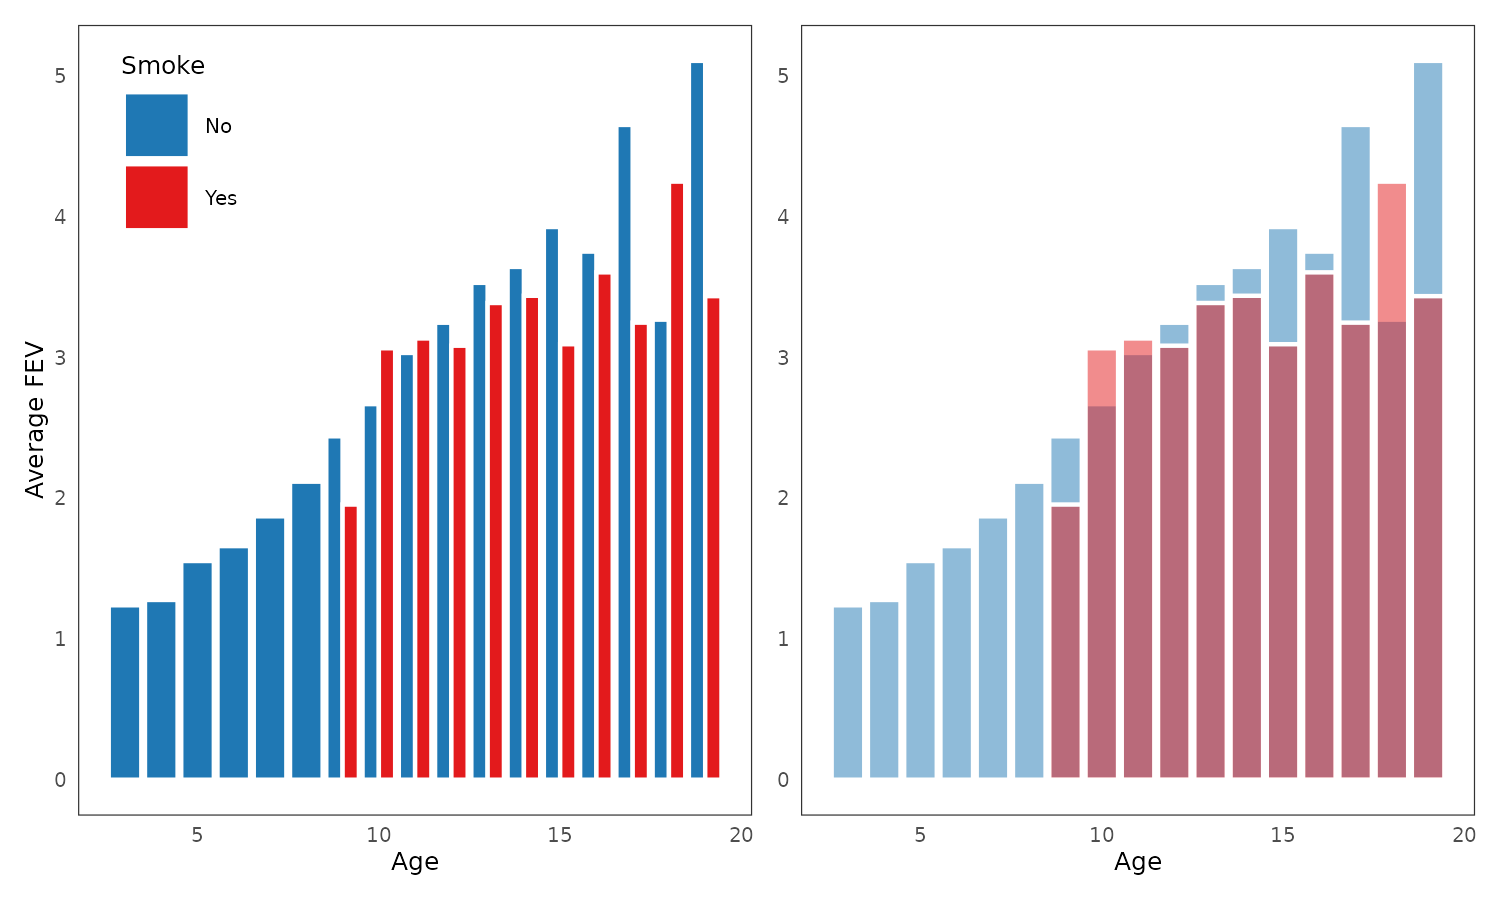
\includegraphics[width=1\linewidth,height=1\textheight]{./figures/grammar-dodging-layering} 

}

\caption{Two alternative means of displaying partitioned data: dodging and layering.}\label{fig:dodging-layering}
\end{figure}

Much has been written about the relative merits of stacking, dodging, and layering. For example, layering is only useful with few categories, as blending many colors can make it difficult to tell the categories apart (\citeproc{ref-franconeri2021}{Franconeri et al. 2021}; \citeproc{ref-wilke2019}{Wilke 2019}). Further, in a landmark study, Cleveland and McGill (\citeproc{ref-cleveland1984}{1984}) showed that people tend to be less accurate when reading information from stacked bar charts as opposed to dodged bar charts. Specifically, since the lower y-axis coordinate of a stacked segment is pushed up by the cumulative height of the segments below, it becomes difficult to accurately compare segments' length, both within and across bars (\citeproc{ref-cleveland1984}{Cleveland and McGill 1984}). Subsequent research has independently validated these findings and expanded upon them (see e.g. \citeproc{ref-heer2010}{Heer and Bostock 2010}; \citeproc{ref-thudt2016}{Thudt et al. 2016}; \citeproc{ref-quadri2021}{Quadri and Rosen 2021}). Due to this suboptimal statistical legibility, many data visualization researchers have urged caution about stacking (see e.g. \citeproc{ref-byron2008}{Byron and Wattenberg 2008}; \citeproc{ref-cairo2014}{Cairo 2014}; \citeproc{ref-franconeri2021}{Franconeri et al. 2021}), and some have even discouraged its use altogether (\citeproc{ref-kosara2016}{Kosara 2016}; \citeproc{ref-wilke2019}{Wilke 2019}).

However, I contend that, while dodging and layering are indeed valuable techniques for static visualization, stacking offers significant advantages in interactive contexts. The issue comes down to how the three techniques represent the relatedness of data subsets. In dodging and layering, the only indication of the fact that two subsets are related is their spatial proximity. In contrast, in stacking, the stacked segments are both close together in space (proximity) and also combine together to form a single object (part-whole relationship, see also \citeproc{ref-slingsby2009}{Slingsby, Dykes, and Wood 2009}). Thus, in a stacked barplot, we can interpret an individual stacked segments as highlighted \emph{parts} of a bar, whereas the same is not true for dodging or layering. This subtle distinction has important implications for the figure's visual properties and interactive behavior (see also \citeproc{ref-roberts2000}{Roberts et al. 2000}; \citeproc{ref-wilhelm2008}{Wilhelm 2008}).

Take, for instance, the typical stacked barplot. Here, the heights of the stacked segments sum to total bar height, providing a fixed upper bound and a clear visual anchor, see Figure \ref{fig:stacking-vs-dodging}. This is particularly useful with linked selection. Even when the segment heights change, the total bar height remains constant, allowing us to maintain a fixed upper y-axis limit, for instance. This leads to predictable plot behavior: the highlighted segments will never ``grow'' outside of the plotting area. Additionally, computational overhead is also reduced, since the axis limits only need to be recomputed \emph{when total bar heights change} (e.g.~changing binwidth in a histogram), not when the segment heights change. These advantages extend beyond barplots: whenever we represent selection by highlighting interior parts of geometric objects, the resulting interaction will behave more ``consistently'' and we can save computational resources by caching the quantities associated with the whole objects.

\begin{figure}

{\centering 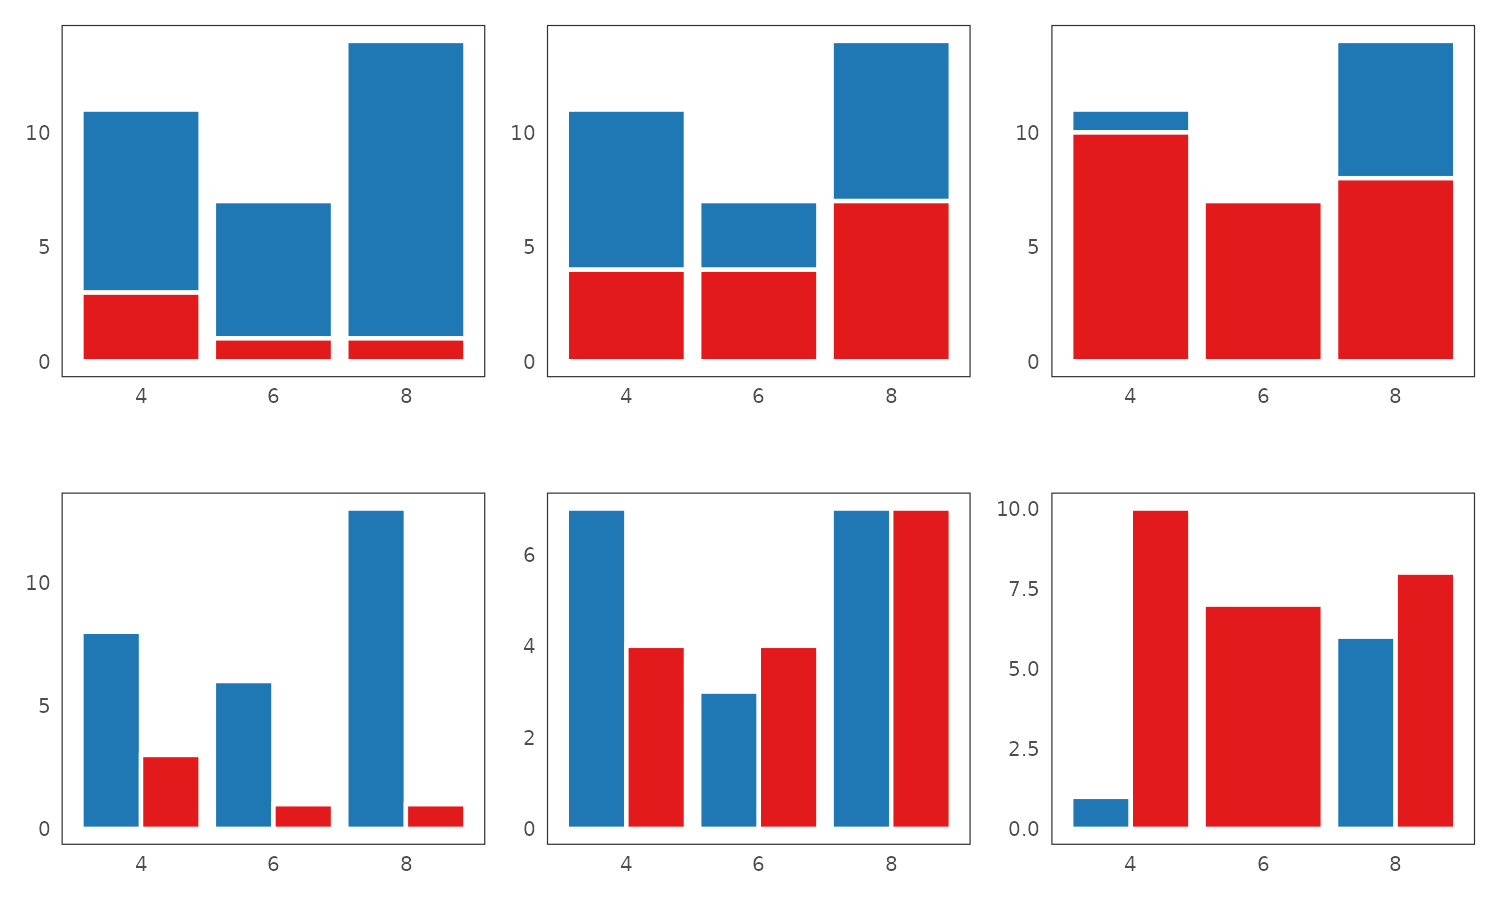
\includegraphics[width=1\linewidth,height=1\textheight]{./figures/stacking-vs-dodging} 

}

\caption{Stacking has advantages over dodging (and layering) when it comes to displaying linked selection. Plots left to right show simulated static snapshots of more cases being selected (red). In a stacked barplot (top row), the heights of the higlighted segments are always bound by the height of the whole bar, and so the outline of the figure remains constant. In contrast, in a dodged barplot, the bar segment heights are not bounded, leading to the outline of the figure fluctuating dramatically (notice the changing upper y-axis limit).}\label{fig:stacking-vs-dodging}
\end{figure}

This is not the case for dodging and layering. Here, the segment heights are unbounded, meaning that heights of the selected segments may exceed those of unselected segments. This forces us to choose between making the upper y-axis limit reactive (losing the context that the limit provides, whenever selection happens), or risking the segments growing outside the plot area. Moreover, I contend that the lack of visual anchoring creates significant visual noise. Research shows that translating and looming stimuli capture attention (\citeproc{ref-franconeri2003}{Franconeri and Simons 2003}). Because selection may translate the top edges of the dodged/layered bar segments in unpredictable ways, it follows that the resulting animation will be more visually distracting and harder to follow.

Surprisingly, little research has explored the perceptual and computational benefits of part-whole object relations. I have been able to find only two relevant references: Wilhelm (\citeproc{ref-wilhelm2008}{Wilhelm 2008}), who discusses the topic in the context of the visual properties of linked selection, and Sievert (\citeproc{ref-sievert2020}{Sievert 2020}), who focuses more on the computational aspects. Given the key importance of this topic to the main ideas of the present thesis, I will examine the content of these two referenes in more detail.

Wilhelm (\citeproc{ref-wilhelm2008}{2008}) outlines three strategies for displaying selection: replacement, overlaying, and repetition. Within the context of the three techniques discussed above (stacking, dodging, and layering), overlaying essentially conflates both stacking and layering, repetition is equivalent to dodging, and replacement involves re-rendering the entire visualization upon selection. Wilhelm notes that replacement is a flawed strategy because it entirely discards contextual information such as axis limits. He also argues that repetition is less commonly used due to the necessity of re-arranging the plot upon selection. Finally, he identifies two issues with overlaying: the fact that plot parameters are inherited from the plot representing the whole data set, and the fact that parts of the original plot may become obscured by the highlighted subset. Ultimately, he appears to favor repetition over the other two methods.

Sievert (\citeproc{ref-sievert2020}{Sievert 2020, chap. 17}), discusses the computational challenges related to rendering linked views with Shiny (\citeproc{ref-shiny2024}{W. Chang et al. 2024}) and \texttt{plotly} (\citeproc{ref-plotly2023}{Plotly Inc. 2023}). He discusses the problem of making comparisons when plot context (provided by parameters such as axis limits) is lost during selection, and mentions how retaining the context of the ``whole bars'' improves computational efficiency, since the entire plot does not have to be re-rendered from scratch. To address this, Sievert provides a solution in the form of a fixed ``base layer'', which he acknowledges ``may seem like a hack'', but provides a better user-experience.

My conclusion aligns fairly closely with Sievert (\citeproc{ref-sievert2020}{2020}), but diverges somewhat from Wilhelm (\citeproc{ref-wilhelm2008}{2008}). Contrary to Wilhelm, I contend that, while overlaying/stacking is less flexible than repetition/dodging, layering, and replacement, it is nevertheless the superior method, since it ensures that the context of the whole data set is always preserved. Conversely, repetition/dodging - the method favored by Wilhelm - suffers from the same contextual information loss as replacement. Specifically, if we draw highlighted subsets as separate objects, then, in the general case, we have to make axis limits reactive. What Wilhelm (\citeproc{ref-wilhelm2008}{2008}) sees as one of the problems with overlaying/stacking - the fact that plot parameters are inherited from the whole data - I instead see as a fundamental strength, similar to Sievert (\citeproc{ref-sievert2020}{2020}). However, unlike Sievert, I go further in positing that something like Sievert's ``fixed'' base layer should not just be an accidental workaround, but instead a fundamental concept in how the data visualization pipeline is structured. Maintaining part-whole relations between geometric objects and highlighted segments ensures that interaction will be computationally efficient and always preserve context.

\subsection{Stackable summaries: A brief journey into Category Theory}\label{stackable-summaries-a-brief-journey-into-category-theory}

Let's briefly recap the key points so far. In section \ref{partitioning}, I advocated for modeling plots as a hierarchy of partitions, particularly a preorder of data subsets ordered by set union. Starting with the full data set, we divide it into disjoint subsets, each corresponding to a geometric object. These subsets can then be further subdivided, representing parts of those objects (such as those resulting from linked selection). As discussed in Section \ref{hierarchy}, we end up with a tree-like structure that encodes this part-whole relationship, which can be formally described as a preorder.

Further, in Section \ref{stacking-not-graphical}, I demonstrated on the example \ref{fig:barplot-maximums} that some ``stackable'' summary statistics have the property of preserving the part-whole relationships in the data hierarchy, whereas others do not. I have also and pointed to other researchers who have noted this problem. Additionally, I have argued that preserving these part-whole relationship in our visualizations is desirable, particularly when interaction is involved. They simplify certain interactive behaviors, make them more intuitive and ``natural,'' and reduce the workload interactive data visualization systems need to do.

Now it is finally time to discuss what makes certain statistics stackable. To do this, I will need to use some concepts from category theory. These concepts are described in greater detail in the \hyperref[mathematical-theory]{Appendix: Mathematical Theory} - the reader is advised to consult this section if they are unfamiliar with the material (links to appropriate sections will also be provided throughout the text). As a final note, although category theory is a very complex field, only introductory concepts - which are sufficient for our purposes - will be used here.

\subsubsection{Generalizing preorders: Categories}\label{preorders-categories}

Previously, I had formalized the hierarchy of data subsets as a preorder, an algebraic concept with a structure that we want to preserve. However, to truly formalize the concept of preserving structure, we need to take one more step towards abstraction. Specifically, it is necessary to recast preorders as categories, a fundamental concept in category theory.

The definition of a \hyperref[categories]{category} is quite straightforward. In simple terms, a category \(\mathcal{C}\) is just a collection of objects, connected by arrows, that conforms to several properties. More specifically, when we have a category \(\mathcal{C}\):

\begin{itemize}
\tightlist
\item
  We have a collection of objects \(\text{Ob}(\mathcal{C})\)
\item
  For every pair of objects \(c_1, c_2 \in \text{Ob}(\mathcal{C})\), there is a set of of arrows (morphisms) \(c_1 \to c_2\) (this set of arrows is often denoted as \(\mathcal{C}(c_1, c_2)\))
\end{itemize}

Further:

\begin{itemize}
\tightlist
\item
  Every object \(c \in \text{Ob}(\mathcal{C})\) has special arrow \(\text{id}_c\) pointing back to itself (called the identity morphism)
\item
  Arrows compose. That is, if there is an arrow \(f\) from object \(c_1\) to object \(c_2\), and an arrow \(g\) from object \(c_2\) to object \(c_3\), we can define a composite arrow \(f ⨾g\) from \(c_1\) to \(c_3\)
\end{itemize}

Finally, the arrows need to conform to two properties:

\begin{itemize}
\tightlist
\item
  Composing with the identity morphism leaves arrows unchanged: \(\text{id}_{c_1} ⨾f = f ⨾\text{id}_{c_2} = f\)
\item
  Composition is associative: \(f ⨾(g ⨾h) = (f ⨾g) ⨾h = f ⨾g ⨾h\)
\end{itemize}

For example, the following is a diagram of a simple category with two objects and a single non-identity morphism, called \(\underline{\textbf{2}}\):

\begin{center}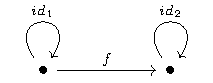
\includegraphics[width=1\linewidth,height=1\textheight]{./figures/category-two} \end{center}

Here, the morphism \(f\) simply means we can get from object 1 (left) to object 2 (right). Based on the rules of a category, we can infer that, for example, \((\text{id}_1 ⨾f) ⨾\text{id}_2 = \text{id}_1 ⨾(f ⨾\text{id}_2) = f\). As a final note, since the identity arrows are always present, they are often not drawn explicitly in diagrams of categories (however, they are presumed to be there).

Now, what are the objects? What are the arrows? That is all left for us to specify. For example, the objects and arrows could be elements of a set and relations, sets and functions, or even entire categories and a generalizations of functions called functors (which we will discuss later). This abstract nature of categories can be initially difficult to grasp. However, there are some fairly straightforward examples that can help.

A key example, relevant to our discussion, are preorders. Specifically, it can be shown that every preorder is in fact a category. Given a preorder on a set \(S\), define the objects \(c \in \text{Ob}(\mathcal{C})\) as the elements in \(s \in S\), and, for any two objects \(c_1\) and \(c_2\), define at most one morphism \(c_1 \to c_2\) if \(c_1 \leq c_2\) (and no morphism if \(c_1 \not \leq c_2\)). Then, the two properties of preorders just fall out of the definition of a category:

\begin{itemize}
\tightlist
\item
  Reflexivity: this is just the identity morphism. For every \(c \in \text{Ob}(\mathcal{C})\), we have \(\text{id}_c : c \to c\)
\item
  Transitivity: this is just composition of morphisms. Given \(f: c_1 \to c_2\) (\(c_1 \leq c_2\)) and \(g: c_2 \to c_3\) (\(c_2 \leq c_3\)), we can define \(h: c_1 \to c_3\) as \(h = f ⨾g\) (\(c_1 \leq c_3\))
\end{itemize}

In our concrete case of preorder of data subsets ordered by set union, we can easily reuse the diagram from Section \ref{plots-as-preorders} - Figure \ref{fig:barplot-preorder2} - and re-intepret it as a category \(\mathcal{D}\):

\begin{center}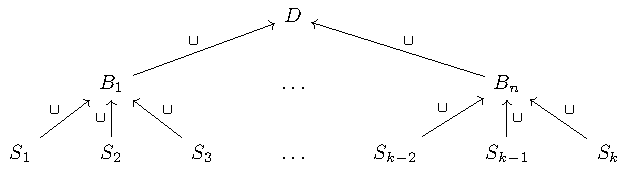
\includegraphics[width=1\linewidth,height=1\textheight]{./figures/barplot-preorder2} \end{center}

Here, the objects are again just the data subsets, such as the whole data set \(D_D\), the bar subsets \(D_{B_i}\), and the segments \(D_{S_j}\). The morphisms are the arrows indicating set union. As before, the fact that there is an arrow between \(D_{S_1}\) and \(D_{B_1}\) simply means that Segment 1 can be combined with another set to form Bar 1 (and the absence of an arrow between \(D_{S_1}\) and \(D_{S_2}\) indicates that segments are disjoint). Identity morphisms are not explicitly shown, but they are of course present (every subset can be combined with the empty set \(\varnothing\) to get back the original set). Finally, as mentioned above, reflexivity and transitivity automatically fall out of the definition of a category.

Further, this categorical definition allows for a more precise description of the relationships in the figure. Whereas in a preorder, the relation is assumed to be homogeneous between all objects, a category allows for distinct morphisms between objects. Thus, instead of simply stating that the relation \(\cup\) represents union with some unspecified set, we can explicitly define it as \emph{union with all other sibling sets} and label the corresponding arrows appropriately. While labeling the entire graph would create visual clutter, the following example demonstrates this approach for a portion of the diagram, specifically the subsets corresponding to Bar 1:

\begin{figure}

{\centering 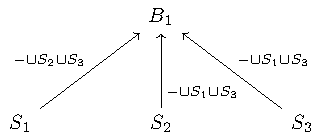
\includegraphics[width=1\linewidth,height=1\textheight]{./figures/barplot-preorder3} 

}

\caption{A diagram of a part of the barplot/spineplot category, with all of the morphisms described explictly.}\label{fig:barplot-preorder3}
\end{figure}

Figure \ref{fig:barplot-preorder3} illustrates the simple fact that Bar 1 is formed by combining the data subset of Segment 1 with those of Segments 2 and 3 using the set union operator (and similarly for Segments 2 and 3). In some way, it is simply a more detailed, zoomed-in view of a section of Figure \ref{fig:barplot-preorder2}. We could in fact go further and add nodes representing pairwise unions of sets, e.g.~\(D_{S_1} \cup D_{S_2}\), however, this is not strictly necessary.

Even though the benefits of re-formulating our data hierarchy in this abstract way may still not be entirely apparent, I encourage the reader to bear with me. In the next sections, I will show the advantages of thinking about our data and visualizations categorically.

\subsubsection{Structure preserving maps: Functors}\label{structure-preserving-maps-functors}

A second fundamental concept in category theory is that of a structure-preserving map or a \hyperref[functors]{functor}. A functor is a mapping from one category to another which preserves the relationships within the first category (this can also be thought of as drawing a diagram of the the first category inside the second category, \citeproc{ref-fong2019}{Fong and Spivak 2019}).

In more precise terms, a functor \(F: \mathcal{C} \to \mathcal{D}\) is a mapping from category \(\mathcal{C}\) to category \(\mathcal{D}\) such that:

\begin{itemize}
\tightlist
\item
  Every object in \(c \in \text{Ob}(\mathcal{C})\) is mapped to some object \(d \in \text{Ob}(\mathcal{D})\)
\item
  Every morphism \(f: c_1 \to c_2\) in \(\mathcal{C}(c_1, c_2)\) is mapped to some morphism in \(\mathcal{D}(F(c_1), F(c_2))\), i.e.~\(F(f): F(c_1) \to F(c_2)\)
\end{itemize}

Further, this mapping is subject to two fundamental properties:

\begin{itemize}
\tightlist
\item
  Identities are preserved: \(F(\text{id}_c) = \text{id}_{F(c)}\)
\item
  Composition is too: \(F(f ⨾g) = F(f) ⨾F(g)\)
\end{itemize}

The first property is fairly intuitive and simply states that objects cannot be separated from their identities. The second property is more interesting, since it tells us that all compositions (chains of arrows) must be preserved. Other than that, we are free to map the objects and arrows as we wish. For instance, we can map multiple objects in \(\text{Ob}(\mathcal{C})\) to a single object in \(\text{Ob}(\mathcal{D})\), ``squish'' a morphism (or a chain of morphisms) in \(\mathcal{C}\) by mapping it to an identity morphism in \(\mathcal{D}\), or ``stretch'' a morphism in \(\mathcal{C}\) by mapping it to a composite morphism in \(\mathcal{D}\). However, we cannot ``rip'' or ``tear'' any morphism or chain of morphisms in \(\mathcal{C}\) into multiple morphisms or chains in \(\mathcal{D}\).

This second property of preserving composition can be described by the following commutative diagram:

\begin{figure}

{\centering 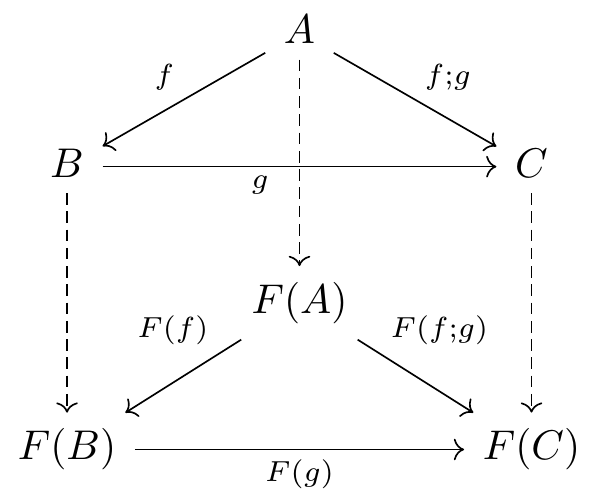
\includegraphics[width=1\linewidth,height=1\textheight]{./figures/functor} 

}

\caption{A commutative diagram showing how a functor $F$ preserves associativity. $A$, $B$, $C$ are objects in category $\mathcal{C}$, $F(A)$, $F(B)$, $F(C)$ are objects in category $\mathcal{D}$, $f$ and $g$ are morphisms in $\mathcal{C}$, and $F(F)$ and $F(g)$ are objects in $\mathcal{D}$.}\label{fig:functor}
\end{figure}

Here, \(A\), \(B\), and \(C\) are three objects in category \(\mathcal{C}\) and \(F(A)\), \(F(B)\), and \(F(C)\) are the same three objects mapped to category \(\mathcal{D}\) (and the same for morphisms \(f\) and \(g\)). The diagram commuting means that following any two parallel arrows (same source and destination) gives us the same result. For instance, to get from \(A\) to \(F(C)\), we may either:

\begin{itemize}
\tightlist
\item
  Map \(A \to C\) (via \(f ⨾g\)) and then apply the functor (\(F(\text{id}_C)\))
\item
  Map \(A \to B\) (via \(f\)), apply the functor (\(F(\text{id}_B)\)), and then map \(F(B) \to F(C)\) (via \(F(g)\))
\item
  Apply the functor immediately (\(F(\text{id}_A)\)) and then map \(F(A) \to F(C)\) (via \(F(f ⨾g) = F(f) ⨾F(g)\))
\end{itemize}

The second property of functors states that all of the above paths must lead to the same object \(F(C)\) (if \(F\) is a functor).

\subsubsection{Aggregation: A functor from the preorder of data subsets to the preorder of summary statistics}\label{aggregation-functor}

As we have established before, when visualizing data, we may start with a category/preorder of data subsets ordered by sibling subset union, as in Figure \ref{fig:barplot-preorder2} (reproduced below for reminder). We would like to translate these data subsets into summary statistics, in a way that preserves the inherent structure in the data. As we will see, the appropriate way to do this is via a functor.

\begin{figure}

{\centering 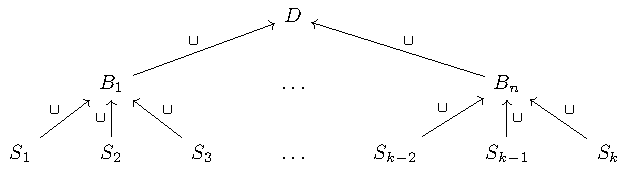
\includegraphics[width=1\linewidth,height=1\textheight]{./figures/barplot-preorder2} 

}

\caption{Reproduction of Figure \\ref{fig:barplot-preorder2}: a diagram of a barplot/spineplot represented as a preorder/category ordered by set union.}\label{fig:barplot-preorder22}
\end{figure}

But first, let's discuss the summary statistics. Since we want to summarize each data subset, then, it is given that we should end up with an equal number of summaries. For instance, if \(D = \{ D_D, D_{B_1}, \ldots D_{B_n}, D_{S_1}, \ldots, D_{S_k} \}\) is the set of data subsets corresponding to the whole data set, bars, and segments, respectively, and \(S\) is the set of summaries, then \(\lvert D \lvert = \lvert S \lvert\). Further, since the elements of \(D\) are actually objects in a category (\(\mathcal{D}\)), then, intuitively, \(S\) should be a part of a category as well, let's call it \(\mathcal{S}\).

If the elements of \(S\) are objects in a category \(\mathcal{S}\), what should be the morphisms? In the category of data subsets \(\mathcal{D}\), the morphisms are given by union with the sibling subsets. In the category of summaries, we want the morphisms to reflect some operation that ``behaves like set union'', such that it represents the operation of \emph{combining sibling summaries}. We can label this operation with the symbol \(\otimes\), such that the resulting category looks as follows:

\begin{figure}

{\centering 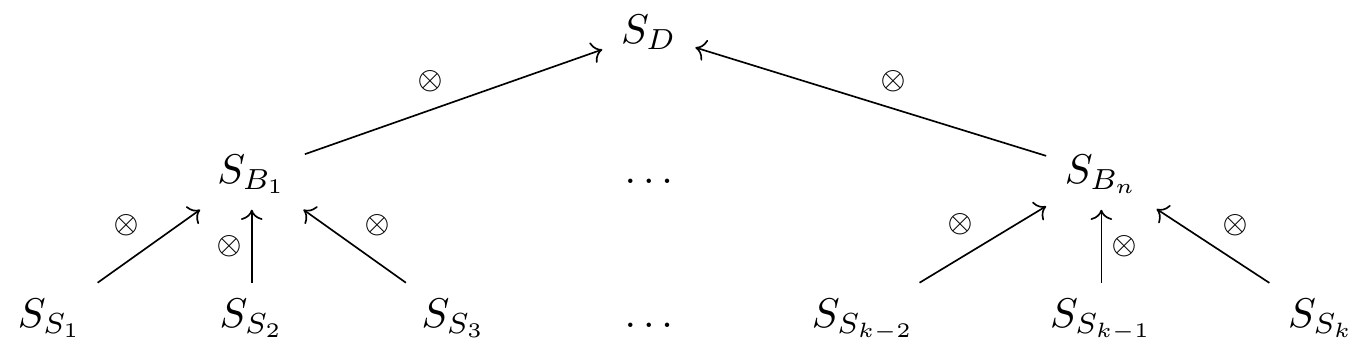
\includegraphics[width=1\linewidth,height=1\textheight]{./figures/barplot-preorder4} 

}

\caption{A diagram of barplot/spineplot summary statistic preorder/category, ordered by the combination operator $\otimes$.}\label{fig:barplot-preorder4}
\end{figure}

As before, each \(\otimes\) in the diagram above corresponds to the operation of combining a summary with the other sibling summaries, such that, for example, the label for the arrow \(S_{S_1} \to S_{B_1}\) should be \(- \otimes S_{S_1} \otimes S_{S_2}\). In words, ``a segment summary combines into a bar summary''.

Now comes the key point. Suppose that we have some summary function \(F: D \to S\) which maps data subsets to summaries. To preserve the structure of \(\mathcal{D}\), the operation should be a functor \(F: \mathcal{D} \to \mathcal{S}\), which maps data subsets in \(D\) to summaries in \(S\) and set unions \(D_i \cup D_j\) to combinations of summaries \(S_i \otimes S_j\), such that composition and identities are preserved. Specifically, by substituting our morphisms into the composition-preserving property of functors:

\[F(- \cup D_{i} ⨾- \cup D_{j}) = F(- \cup D_i) ⨾F(- \cup D_j)\]

The expression above appears somewhat awkward due to the mixing of function expressions with the binary operator \(\cup\) and the composition operator \(⨾\) (i.e.~if instead of \(- \cup D_i\) and \(- \cup D_j\) we had \(f\) and \(g\), the expression \(F(f ⨾g) = F(f) ⨾F(g)\) would look much cleaner, even though it expresses the same concept). However, it can be greatly simplified by noting two facts:

\begin{itemize}
\tightlist
\item
  \(F(- \cup D_i ) = - \otimes F(D_i)\). This follows from the definition of our functor: the union operator is mapped to combining summaries in the summary category.
\item
  We can omit the composition operator \(⨾\). This is due to the fact that \(\cup\) and \(\otimes\) are associative binary operators (associativity follows from the definition of composition in categories). As an example, if \(f(x) = - \otimes 2 = x + 2\), then we can write \([f ⨾f](x) = f(f(x)) = ((x + 2) + 2) = x + 2 + 2\))
\end{itemize}

This leads to the following simplification:

\[F(- \cup D_i \cup D_j) = - \otimes F(D_i) \otimes F(D_j)\]

Finally, without loss of generality, we can choose the empty set \(\varnothing\) as the subset being operated on (\(-\)), and then the equation reduces to:

\begin{equation}

F(D_i \cup D_j) = F(D_i) \otimes F(D_j)
\label{eq:summary-functor-composition}

\end{equation}

In other words, when summarizing data, \emph{it should not matter whether we first take the union of the underlying data and then summarize the resulting superset, or first summarize the subsets and then combine the summaries via the combination operator \(\otimes\) (i.e.~the summary should distribute across set union)}.

Finally, we should note that, to be fully functorial, the operation should also preserve identities:

\begin{equation}

F(\text{id}_{D_i}) = \text{id}_{F(D_i)}
\label{eq:summary-functor-identity}

\end{equation}

\subsubsection{Functorial summaries and set union}\label{functorial-summaries-and-set-union}

Let's explore the functoriality of summary statistics in more concrete terms. First, as was mentioned in Section \ref{plots-as-preorders}, the identity morphism for a data subset is just union with the empty set, \(- \cup \varnothing\). Therefore, preserving identities as per Equation \eqref{eq:summary-functor-identity} amounts to:

\begin{align}

F(\text{id}_{D_i}) &= F(D_i \cup \varnothing) \\
                   &= F(D_i) \otimes F(\varnothing) \\ 
                   &= F(D_i) \otimes e \\
                   &= F(D_i) = \text{id}_{F(D_i)}
\end{align}

This means that the summary operation \(F\) must be defined for the empty set, and should return some ``neutral'' element \(e = F(\varnothing) \in S\), which, when combined with any other summary, just returns the same summary back.

Second, as per Equation \eqref{eq:summary-functor-composition}, the summary should distribute across set union via the combination operator \(\otimes\):

\[F(D_i \cup D_j) = F(D_i) \otimes F(D_j)\]

This distributive property should hold over \emph{all} disjoint subsets of the data as these correspond to all possible arrows we can draw in the set union diagram of the data subset preorder (Figure \ref{fig:barplot-preorder2}). Further, given any set \(D_i \in D\), the smallest possible (non-empty) disjoint subset is a single data point (row) \(d_j \in D_i\). Thus, the summary operation should distribute over individual data points:

\[F(d_1 \cup d_2 \cup \ldots \cup d_n) = F(d_1) \otimes F(d_2) \otimes \ldots \otimes F(d_n)\]

Thus, from a certain point of view, \(F\) \emph{is} the binary combination operator \(\otimes\)\footnote{Technically, if \(d_i\) represents a single data row, with multiple named data values corresponding to columns, the summary operation \(F\) should also select the appropriate value(s) while remaining closed under repeated applications. For instance, if we are summarizing a variable named \texttt{x}, the following R function fullfills these criteria: \texttt{pick\_sum\ \textless{}-\ function(s,\ d)\ ifelse(is.numeric(d),\ s\ +\ d,\ s\ +\ d\$x);\ Reduce(pick\_sum,\ lapply(1:3,\ \textbackslash{}(n)\ list(x\ =\ n)),\ 0)}.}. With a bit of handwaving, we can write:

\[F(d_1 \cup d_2 \cup \ldots d_k) = d_1 \otimes d_2 \otimes \ldots d_n\]

Just to drive the point home, we can also follow the equality the other way, starting with combining the summaries of two data subsets \(F(D_i)\) and \(F(D_j)\). Then:

\begin{align}

F(D_i) \otimes F(D_j) &= (d_{i1} \otimes d_{i2} \otimes \ldots d_{in}) \otimes (d_{j1} \otimes d_{j1} \otimes \ldots d_{jk}) \\
&= d_{i1} \otimes d_{i2} \otimes \ldots d_{in} \otimes d_{j1} \otimes d_{j1} \otimes \ldots d_{jk} \qquad \text{(by associativity)} \\
&= F(D_i \cup D_j)

\end{align}

Again, this shows that combining summaries leads to a valid summary of the underlying set union, which is precisely the desired property we set out to find.

Finally, we can also consider the case when \(F\) is \emph{not} functorial, i.e.~\(F(D_i \cup D_j) \neq F(D_i) \otimes F(D_j)\). This corresponds to a situation where the summary of the superset somehow contains some additional ``non-additive'' information that the summaries of either of the two subsets do not. More generally, these situation where the \emph{whole is more than ``sum'' of its parts} are called an \emph{interactive} or \emph{generative effects} (\citeproc{ref-adam2017}{Adam 2017}; \citeproc{ref-fong2019}{Fong and Spivak 2019}). Generative effects apply to a broader class of mappings than just the specific case with set union we have outlined here, however, the idea of (not) preserving composition (\(F(f ⨾g) \neq F(f) ⨾F(g)\)) is the same. For our summary statistics to be well-behaved under features like linked selection, they should \emph{not} have any kind of generative effect.

\subsubsection{Whole equal to the sum of its parts: Monoids}\label{whole-equal-to-the-sum-of-its-parts-monoids}

Above, I have argued that, for plots to be well-behaved under certain kinds of interactions such as linked selection, the summary statistics we display should \emph{``behave like set union''}. Specifically, they should be a functor from the preorder of data subsets, such that combining two summaries gives the same result as summarizing the union of the underlying data. Conversely, the summary of the union should result in no non-additive ``surprises'' or generative effects.

The framing of the summary mapping \(F\) as functor has lead to two key insights: the summary statistic should be based on some binary associative operation \(\otimes\), and the summarized values should be equipped with some ``neutral'' value that is the result of summarizing an empty set. It turns out there is a well-known algebraic structure with these exact properties: a monoid.

Formally, a monoid \((M, e, \otimes)\) is a set \(M\) equipped with a binary operation \(\otimes\) and a special neutral element \(e\), such that the operation is:

\begin{itemize}
\tightlist
\item
  Unital: \(m \otimes e = e \otimes m = m\) for all \(m \in M\)
\item
  Associative: \((m_1 \otimes m_2) \otimes m_3 = m_1 \otimes (m_2 \otimes m_3) = m_1 \otimes m_2 \otimes m_3\)
\end{itemize}

These are exactly the properties we were looking for. In other words, if the summary statistic is a monoid, it behaves like set union. The summary functor \(F\) then just acts the following way:

\begin{itemize}
\tightlist
\item
  For the empty set, it just returns the neutral value: \(F(\varnothing) = e\)
\item
  For a non-empty set \(D_i\), it ``folds'' the set by repeatedly applying the combination operator: \(F(D_i) = F(\{d_{i1} , d_{i2}, \ldots, d_{in} \}) = d_{i1} \otimes d_{i2} \otimes \ldots \otimes d_{in}\)
\end{itemize}

Monoids are well-known in category theory and functional programming. When \(M\) is the set of real numbers, a typical example is the summation \((\mathbb{R}, 0, +)\) (which we are familiar with as the ``default'' summary statistic in typical barplots). Other examples include the product \((\mathbb{R}, 1, \cdot)\) and maximum operators \((\mathbb{R}, \max, -\infty)\). However, the set \(M\) does not have to be only numbers. For example, the set of strings with the concatenation operator \(\text{++}\) and the empty string \(\text{""}\) as the neutral element forms a valid monoid:

\[\text{"hello" ++ ""} = \text{"" ++ "hello" } = \text{"hello"} \]
\[\text{"quick " ++ (" brown" ++ " fox")}  \text{} = \text{("quick " ++ " brown ") ++ " fox"} = \text{"quick brown fox"}\]

While most summary statistics we care about in data visualization are quantitative, the fact that some non-numeric data summaries can behave like set union may be still interesting to ponder.

Further, even the set union \(\cup\) operation itself forms a monoid, with the empty set \(\varnothing\) as the neutral/identity element. Thus, in a certain way, the mapping of data subsets to summaries \(F\) can be seen as a mapping between two monoids: a \emph{monoid homomorphism} (which is just an abstract algebra term for a functor between monoids). However, \(F\) is more than just a monoid homomorphism; monoids alone do not capture the hierarchical structure of \(\mathcal{D}\) and \(\mathcal{P}\). Instead, \(F\) is a mapping between two categories that have the features of both a monoid \emph{and} preorder. As a sidenote, the technical term for a monoid that is also a preorder is, unsurprisingly, a \emph{monoidal preorder} (\citeproc{ref-nlab2024e}{nLab 2025}). Thus, \(F\) could technically be called a \emph{``monoidal preorder homomorphism''}. However, I believe it is far easier and clearer to simply refer to \(F\) as a functor.

As a final note, a key consequence of the associativity of monoids is linerizability. Specifically, an arbitrary expression built with an associative binary function \(f\), e.g.~\(f(f(x, y), f(z, f(u, w)))\) can always be rewritten as a linear sequence of steps (e.g.~\(f(x, f(y, f(z, f(u, w))))\)). This effectively flattens the expression tree into a linear chain (\citeproc{ref-adam2017}{Adam 2017}).

\subsubsection{Monoids in code}\label{monoids-in-code}

Monoids translate well to code and are in fact frequently used in functional programming (see e.g. \citeproc{ref-milewski2018}{Milewski 2018}; \citeproc{ref-stepanov2014}{Stepanov and Rose 2014}). Further, we can even test whether an arbitrary summary function conforms to our specific functorial properties. For instance, in R, if we replace the set union operation with vector/array concatenation (the \texttt{c()} function), and provided that we have some three representative data vectors \texttt{x}, \texttt{y}, and \texttt{z}, we can test associativity as follows:

\begin{Shaded}
\begin{Highlighting}[]
\NormalTok{x }\OtherTok{\textless{}{-}} \DecValTok{1}\SpecialCharTok{:}\DecValTok{10}
\NormalTok{y }\OtherTok{\textless{}{-}} \DecValTok{11}\SpecialCharTok{:}\DecValTok{20}
\NormalTok{z }\OtherTok{\textless{}{-}} \DecValTok{21}\SpecialCharTok{:}\DecValTok{30}

\CommentTok{\#     F(f; g)       =     F(f);F(g)}
\FunctionTok{sum}\NormalTok{(}\FunctionTok{c}\NormalTok{(}\FunctionTok{c}\NormalTok{(x, y), z)) }\SpecialCharTok{==} \FunctionTok{sum}\NormalTok{(}\FunctionTok{c}\NormalTok{(}\FunctionTok{sum}\NormalTok{(}\FunctionTok{c}\NormalTok{(x, y)), z))}
\FunctionTok{mean}\NormalTok{(}\FunctionTok{c}\NormalTok{(}\FunctionTok{c}\NormalTok{(x, y), z)) }\SpecialCharTok{==} \FunctionTok{mean}\NormalTok{(}\FunctionTok{c}\NormalTok{(}\FunctionTok{mean}\NormalTok{(}\FunctionTok{c}\NormalTok{(x, y)), z))}
\end{Highlighting}
\end{Shaded}

\begin{verbatim}
## [1] TRUE
## [1] FALSE
\end{verbatim}

Likewise, we can easily test the unitality property with a given neutral element \texttt{e}. We could even create a wrapper function to test whether a given function with a neutral element forms monoid:

\begin{Shaded}
\begin{Highlighting}[]
\NormalTok{is\_unital }\OtherTok{\textless{}{-}} \ControlFlowTok{function}\NormalTok{(fn, e, x) \{}
  \CommentTok{\# Test two{-}sided unitality}
\NormalTok{  (}\FunctionTok{fn}\NormalTok{(}\FunctionTok{c}\NormalTok{(e, x)) }\SpecialCharTok{==} \FunctionTok{fn}\NormalTok{(}\FunctionTok{c}\NormalTok{(x, e))) }\SpecialCharTok{\&\&}\NormalTok{ (}\FunctionTok{fn}\NormalTok{(}\FunctionTok{c}\NormalTok{(e, x)) }\SpecialCharTok{==} \FunctionTok{fn}\NormalTok{(x))}
\NormalTok{\}}

\NormalTok{is\_associative }\OtherTok{\textless{}{-}} \ControlFlowTok{function}\NormalTok{(fn, x, y, z) \{}
  \FunctionTok{fn}\NormalTok{(}\FunctionTok{c}\NormalTok{(}\FunctionTok{c}\NormalTok{(x, y), z)) }\SpecialCharTok{==} \FunctionTok{fn}\NormalTok{(}\FunctionTok{c}\NormalTok{(}\FunctionTok{fn}\NormalTok{(}\FunctionTok{c}\NormalTok{(x, y)), z))}
\NormalTok{\}}

\NormalTok{is\_monoid }\OtherTok{\textless{}{-}} \ControlFlowTok{function}\NormalTok{(fn, e, x, y, z) \{}
  \FunctionTok{is\_unital}\NormalTok{(fn, e, x) }\SpecialCharTok{\&\&} \FunctionTok{is\_associative}\NormalTok{(fn, x, y, z)}
\NormalTok{\}}

\NormalTok{string\_concat }\OtherTok{\textless{}{-}} \ControlFlowTok{function}\NormalTok{(x) }\FunctionTok{paste0}\NormalTok{(x, }\AttributeTok{collapse =} \StringTok{""}\NormalTok{)}
\NormalTok{l2\_norm }\OtherTok{\textless{}{-}} \ControlFlowTok{function}\NormalTok{(x) }\FunctionTok{sqrt}\NormalTok{(}\FunctionTok{sum}\NormalTok{(x}\SpecialCharTok{\^{}}\DecValTok{2}\NormalTok{)) }\CommentTok{\# Aka euclidean norm/vector length}

\FunctionTok{is\_monoid}\NormalTok{(sum, }\DecValTok{0}\NormalTok{, x, y, z)}
\FunctionTok{is\_monoid}\NormalTok{(max, }\SpecialCharTok{{-}}\ConstantTok{Inf}\NormalTok{, x, y, z)}
\FunctionTok{is\_monoid}\NormalTok{(prod, }\DecValTok{1}\NormalTok{, x, y, z)}
\FunctionTok{is\_monoid}\NormalTok{(string\_concat, }\StringTok{""}\NormalTok{, }\StringTok{"a"}\NormalTok{, }\StringTok{"b"}\NormalTok{, }\StringTok{"c"}\NormalTok{)}
\FunctionTok{is\_monoid}\NormalTok{(l2\_norm, }\DecValTok{0}\NormalTok{, x, y, z)}
\FunctionTok{is\_monoid}\NormalTok{(mean, }\DecValTok{0}\NormalTok{, x, y, z)}
\FunctionTok{is\_monoid}\NormalTok{(median, }\DecValTok{0}\NormalTok{, x, y, z)}
\FunctionTok{is\_monoid}\NormalTok{(sd, }\DecValTok{0}\NormalTok{, x, y, z)}
\end{Highlighting}
\end{Shaded}

\begin{verbatim}
## [1] TRUE
## [1] TRUE
## [1] TRUE
## [1] TRUE
## [1] TRUE
## [1] FALSE
## [1] FALSE
## [1] FALSE
\end{verbatim}

A couple of points. First, based on what we have shown before, we could simplify our task by defining \texttt{fn} to always take two scalar arguments instead of a vector. This binary formulation would demonstrate that, for example, \texttt{mean2\ ==\ median2\ ==\ function(x,\ y)\ (x\ +\ y)\ /\ 2} (median of even number of elements is the average of the middle two), and so if we can show that \texttt{(x\ +\ y)\ /\ 2} is not associative, we disprove both \texttt{mean2} and \texttt{median2} being a monoid. Also, more intuitively, with three or more values, applying \texttt{median2} amounts to repeatedly averaging values pairwise, and this operation is clearly different from simply picking the middle value. Furthermore, the binary formulation of \texttt{fn} also makes the absence of a neutral element \texttt{e} clearer. For instance, it is not difficult to see that there is no (constant) value \texttt{e} such that \texttt{(x\ +\ e)\ /\ 2\ ==\ x} for all \texttt{x}. Thus, generally, it might make more sense to always formulate \texttt{fn} as a binary function; however, in the code block above, I used the vector formulation to ensure consistency with function definitions of \texttt{mean}, \texttt{median}, and \texttt{sd}.

Second, the properties of associativity and unitality should hold for \emph{all} possible values. Thus, testing that a function passes the \texttt{is\_monoid} test for any three specific values is not sufficient to demonstrate that it is a monoid. For instance, while it is the case that \texttt{mean(c(c(2,\ 4),\ 3))\ ==\ mean(c(mean(c(2,\ 4)),\ 3))}, this does not prove that \texttt{mean} is associative (in fact, with a bit of high-school algebra, it can be shown that the equality holds for any triplets \(x, y, z\) where \(3x + 3y + 6z = 4x + 4y + 4z\)). However, a single counter-example \emph{does} disprove that the summary function is monoid, as is the case, for example, with \texttt{mean}, \texttt{median}, and \texttt{sd} functions above. Thus, while not a hard-and-fast rule, the \texttt{is\_monoid} function can nevertheless be useful for some basic sanity checks about the suitability of certain summary statistics.

\subsubsection{Groups and inverses}\label{groups-and-inverses}

Suppose we have our summary functor \(F\) which summarizes a data subset \(D_i\) by repeatedly applying some monoidal operation \(\otimes\). As we have shown, given two data subsets \(D_i\) and \(D_j\), \(F(D_i) \otimes F(D_j) = F(D_i \cup D_j)\). More concretely, with data subsets \(D_1, D_2, D_3, \ldots\), it is the case that, for example:

\begin{align}

&F(D_1) = F(D_1) \\
&F(D_1) \otimes F(D_2) = F(D_1 \cup D_2) \\
&F(D_1) \otimes F(D_2) \otimes F(D_3) = F(D_1 \cup D_2 \cup D_3) \\
&F(D_1) \otimes F(D_2) \otimes F(D_3) \otimes \ldots = F(D_1 \cup D_2 \cup D_3 \cup \ldots)

\end{align}

Now, comparing the statistic \(F(D_1)\) with \(F(D_1) \otimes F(D_2)\) amounts to comparing the summaries of \(D_1\) with that of \(D_1 \cup D_2\). For instance, in a barplot where \(D_{S_1}\) and \(D_{S_2}\) represent segment subsets that together form a bar subset, \(D_{B_1} = D_{S_1} \cup D_{S_2}\), comparing \(F(D_{S_1})\) and \(F(D_{S_1}) \otimes F(D_{S_2})\) amounts to comparing the summary on the subset \(D_{S_1}\) with that of \(D_{S_1} \cup D_{S_2}\), i.e.~the summary of all cases in the bar.

Why is this important? It is critical to note that \emph{comparing \(D_i\) with \(D_i \cup D_j\) is different from comparing \(D_i\) with \(D_j\) directly}. That is, while \(F(D_i) \otimes F(D_j) = F(D_i \cup D_j)\) is a valid summary of \(D_i \cup D_j\), \emph{there is no guarantee that we will be able to recover \(F(D_j)\) from it}. \(F(D_i) \otimes F(D_j)\) may collapse information contained in \(F(D_i)\) and \(F(D_j)\) individually. If we want to use the combined summary \(F(D_i \cup D_j)\) to compare \(D_i\) and \(D_j\) \emph{as disjoint subsets}, then we also require the presence of an inverse operator \(\otimes^{-1}\):

\[F(D_i) \otimes F(D_j) = F(D_i \cup D_j) \iff F(D_i \cup D_j) \otimes^{-1} F(D_j) = F(D_i)\]

Specifically, we want some inverse operator \(\otimes^{-1}\) that would allow our statistic \emph{to also preserve/distribute over set difference} (\(\setminus\)). Specifically, we could imagine taking the diagram in Figure \ref{fig:barplot-preorder2} and adding a second set of arrows pointing in the opposite direction, labeled with \(\setminus\). Then, for \(F\) to be a functor, it would have to preserve the composition of these set difference arrows as well.

Fortunately, we do not have to search for a monoid with an inverse operator; this is precisely the definition of another famous algebraic structure: a group. Groups are well-studied in group theory and subject to many interesting results (see e.g., \citeproc{ref-pinter2010}{Pinter 2010}). However, for our purposes, a group is just a monoid equipped with the inverse operator \(\otimes^{-1}\), subject to\footnote{The inverse operator needs to be two-sided, since so is set difference.}:

\[x \otimes y = z \iff (z \otimes^{-1} x = y) \wedge (z \otimes^{-1} y = x)\]

When the inverse operator is not present, we can still compare \(D_i\) with \(D_i \cup D_j\), however, direct comparisons of \(D_i\) and \(D_j\) may no longer be possible after combining with \(\otimes\). For instance, a typical example of a monoid which lacks inverse is the maximum operator. It is easy to show that maximum is associative:

\[\max(x, \max(y, z)) = \max(\max(x, y), z)\]

And it also has a neutral element, namely \(-\infty\), thus maximum is a valid monoid. However, maximum lacks an inverse \(\otimes^{-1}\):

\[\not \exists \otimes^{-1} \text{ s. t. } \max(x, y) \otimes^{-1} y = x\]

Thus, for example, if it is the case that:

\[\max(x, y) = 8\]

Then, even if we know that \(y = 8\), there is no way to recover the value of \(x\). Thus, in a certain sense, maximum irretrievably discards information contained in its operands. This is different from generative effects/not preserving composition/lack of associativity, which is about validity: a maximum of maximums is always equal to the maximum of all cases. It is just that there is no meaningful way to ``subtract'' from a maximum: once we choose the larger value, the smaller is lost.

This abstract distinction between groups and monoids, and the presence (absence) of inverses translates into tangible differences in interactive behavior. When implementing linked selection, some interactive systems allow the user to define only a single selection group, whereas others allow multiple. This seemingly minor difference in implementation has a large impact on the kinds of statistics we are able to effectively represent. Specifically, with single-group selection, the user defines a single ``special'' subset that is then compared against the entirety of the data, i.e.~a highlighted subset \(D_i\) that is compared against some superset \(D_j \supseteq D_i\). Crucially, the ``rest'' of the data, \(D_j \setminus D_i\), plays a secondary role: we only care about it in as much as it contributes to the superset \(D_j\). As such, it is enough if the combination operator \(\otimes\) is a part of a monoid. However, in multi-group selection, we actually care about comparing the individual disjoint subsets \(D_i, D_j, D_k, \ldots\) that result from selection. Thus, we require the inverse operator \(\otimes^{-1}\) and \(\otimes\) needs to be a part of a group.

Thus, monoids and groups present two fundamentally different models for linked selection. If we care about using parts of a geometric object to compare some ``special'' highlighted subset \(D_i\) against the subset representing the rest of the data \(D_j \supseteq D_i\), then it is enough for the underlying summary statistic to be a monoid. However, if \(D_i\) and \(D_j\) are disjoint, \(D_i \cap D_j = \varnothing\), and we care about comparing \(D_i\) and \(D_j\) directly, then we also need the inverse operator \(\otimes^{-1}\) and the underlying summary needs to be a group.

This distinction even has interesting implications for data interpretation. For instance, the reason why the maximum operator works well in Figure \ref(fig:barplot-maximums) is because we are comparing a ``special subset'' of the study participants (``smokers'') against that of all participants (``smokers \emph{and} non-smokers''). In other words, with the smoking status variable, it makes sense to compare one category with a union of both. This is not the case for all categorical variables, however. For instance, with a gender variable, it would rarely make sense to think of ``men'' as a special subset of ``men and women'', or vice versa; the vast majority of time, we are interested in comparing men and women directly, as disjoint subsets. Conversely, this is also the case why monoids work with single-group linked selection: the selected points really are a ``special'' subset, and the subset representing the ``rest'' of the data is only interesting in that it is part of ``all'' of the data points to compare against. However, with multiple selection groups, disjoint comparisons become essential.

\subsubsection{Transforming summaries: Stacking, normalizing, and shifting}\label{transforming-summaries-stacking-normalizing-and-shifting}

Finally, once we have computed our tree/category of summaries \(\mathcal{S}\) via the functor \(F: \mathcal{S} \to \mathcal{D}\), we may also need to transform these summaries further, while respecting the structure of the tree. Indeed, such is the precise nature of stacking, as well as normalization in plots such as spineplots and spinograms.

Specifically, consider the diagram of \(\mathcal{S}\) again:

\begin{figure}

{\centering 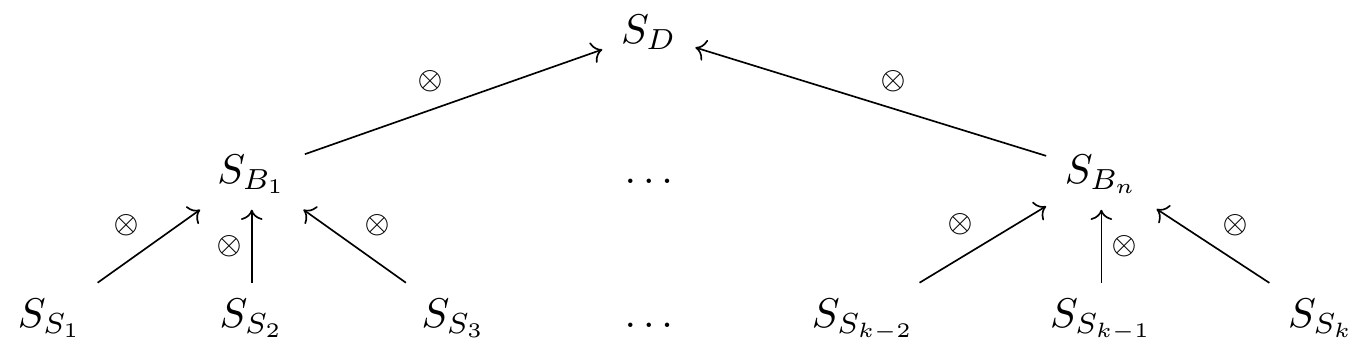
\includegraphics[width=1\linewidth,height=1\textheight]{./figures/barplot-preorder4} 

}

\caption{Reproduction of Figure \\ref{fig:barplot-preorder4}: a diagram of barplot/spineplot summary statistic preorder/category, ordered by the combination operator $\otimes$.}\label{fig:unnamed-chunk-33}
\end{figure}

\paragraph{Stacking}\label{stacking}

To stack statistics, we need to apply our summary/combination operator \(\otimes\) cumulatively, across the child nodes corresponding to the object we want to stack. For instance, in a typical barplot, to stack summaries of segments into the summary of single whole bar \(S_{B_i}\), we can cumulatively sum the child/segment summaries (sums or counts). More specifically, to compute the summaries underlying a stacked bar \(B_1\), we compute \(S_{S_1}\), \(S_{S_1} + S_{S_2}\), \(S_{S_1} + S_{S_2} + S_{S_3}, \ldots\), and so on. To turn this ``typical'' barplot into barplot of maximums (Figure \ref{fig:grammar-barplot-maximums}), we can simply replace the sum operator with the maximum operator: e.g., compute \(S_{S_1}\), \(\max(S_{S_1}, S_{S_2})\), \(\max(\max(S_{S_1}, S_{S_2}), S_{S_3}), \ldots\). As shown before, the properties of monoids ensure that the stacked summary is a valid summary of the underlying set, \(S_{S_1} \otimes S_{S_2} \otimes S_{S_3} \otimes \ldots = S_{B_1}\).

Importantly, stacking can be applied at different levels of the hierarchical structure. Spinograms provide a good example. In spinograms, segments are stacked vertically, within bars, and also bars are stacked horizontally, to form the monolithic rectangle corresponding to the whole data set. Thus, on top of segment-stacking, e.g., \(S_{S_1} \otimes S_{S_2} \otimes S_{S_3} \otimes \ldots = S_{B_1}\), we also have whole-object-stacking, \(S_{B_1} \otimes S_{B_2} \otimes S_{B_3} \otimes \ldots = S_{D}\).

Similar to stacking multiple selection groups, horizontally stacking summary statistics that lack the inverse operator may produce some rather bizzare-looking spinograms. For instance, if we stack maximums and the first histogram bin contains the greatest data value, then the spinogram will consist of only a single bar (all of the bar values stack to the same value). Nevertheless, the plot will be a valid summary of the underlying data. Again, the underlying issue is the lack of the inverse operator and the distinction between monoids and groups.

\paragraph{Normalizing}\label{normalizing}

To normalize statistics, we can apply a binary function that takes as the second argument the value of the parent statistic. For instance, if we have some already stacked segments, e.g.~\(S_{S_1}\), \(S_{S_1} + S_{S_2}\), \(S_{S_1} + S_{S_2} + S_{S_3}\), we can normalize them between {[}0, 1{]} by dividing by the parent bar statistic: \(S_{S_1} / S_{B_1}\), \((S_{S_1} + S_{S_2}) / S_{B_1}\), \((S_{S_1} + S_{S_2} + S_{S_3}) / S_{B_1}\). Thus, as was mentioned in Section \ref{hierarchy}, we need the hierarchical structure to divide \emph{across the levels of the hierarchy}.

It is worth considering whether functions other than simple division could serve as ``normalizing'' functions. For example, weighted division (e.g.~\(\sqrt{S_{S_1}} / \sqrt{S_{B_1}}\)) could be used to down-weigh large values. It may also possible to apply a binary function that is entirely different from division. To be fair, these alternative ways of normalizing data may result in plots which are difficult to interpret, and I have not been able to come up with a real, practical application. Nevertheless, this alternative view of normalization does present intriguing possibilities.

\paragraph{Shifting}\label{shifting}

One final point to mention is that the monoidal structure of the summary statistics presents the possibility of ``shifting'' values towards the neutral element. For instance, with a list of sums (e.g.~\(\{ 4, 2, 3, 2 \}\)), we may use the neutral element (0) to ``shift the values leftwards'' (\(\{ 0, 4, 2, 3 \}\)). This is useful, for example, when horizontally stacking values in a spinogram, since it ensures we have a way to represent the left edge of the first bar (the \texttt{x0} aesthetic). For instance, if we stacked bars horizontally using the cumulative product, e.g.~\(\{ 4, 2, 3, 2 \} \to \{ 4, 8, 24, 48 \}\), then we want the statistics for the left edge of the bars to be \(\{ 1, 4, 8, 24, \}\) (notice that the first value - the neutral element - is 1; also, the right edge will be just the stacked summaries, \(\{ 4, 8, 24, 48 \}\)).

Again, while the practical utility of this technique beyond spineplots and ``typical'' statistics like sums and counts may be limited, it does expand the way we may think about the relationship between summary statistics and our graphs. The existence of a well-defined ``zero-point'' is also useful more generally, for instance, when setting the lower y-axis limit in a barplot.

\section{Scaling and encoding}\label{scaling}

Suppose we have partitioned our data and computed all relevant summary statistics. Now we need a way to to encode these summaries into visual attributes that we can then present on the computer screen. In most data visualization systems, this is done by specialized components called scales or coordinate systems (see e.g. \citeproc{ref-murrell2005}{Murrell 2005}; \citeproc{ref-wickham2016}{Wickham 2016}; \citeproc{ref-wilkinson2012}{Wilkinson 2012}; \citeproc{ref-petricek2020}{Petricek 2020}).

As discussed in Sections \ref{scales-measurement} and \ref{visual-perception}, there exists is a fair amount of literature on the theoretical properties of scales and their relationship to the mechanisms of visual perception (see e.g. \citeproc{ref-krzywinski2013}{Krzywinski 2013}; \citeproc{ref-michell1986}{Michell 1986}; \citeproc{ref-wilkinson2012}{Wilkinson 2012}; \citeproc{ref-stevens1946}{Stevens 1946}). However, when it comes to applying this knowledge and implementing scales in concrete data visualization systems, few research papers are available, and most only discuss the problem in vague, abstract terms (for some rare counter-examples, see e.g. \citeproc{ref-murrell2005}{Murrell 2005}; \citeproc{ref-ziemkiewicz2009}{Ziemkiewicz and Kosara 2009}). To learn about how to actually implement scales scales, one has to go digging through open-source code repositories, which are rarely the most concise educational resources.

This gap between theory and practice is quite unfortunate in my opinion, since scales are an integral part of the data visualization pipeline. Further, they are the foundation of many interactive features, such as zooming, panning, and reordering. Finally, within existing data visualization systems, it is often the case that a large portion of the code is dedicated to scales. For instance, within the \texttt{ggplot2} codebase, the file containing the definition of the \texttt{Scale} class has the greatest number of lines, by quite a significant margin (as of 4th of December 2024, \citeproc{ref-ggplot2repo2024}{Wickham 2024}), see Figure \ref{fig:ggplot2-linecounts}:

\begin{figure}

{\centering 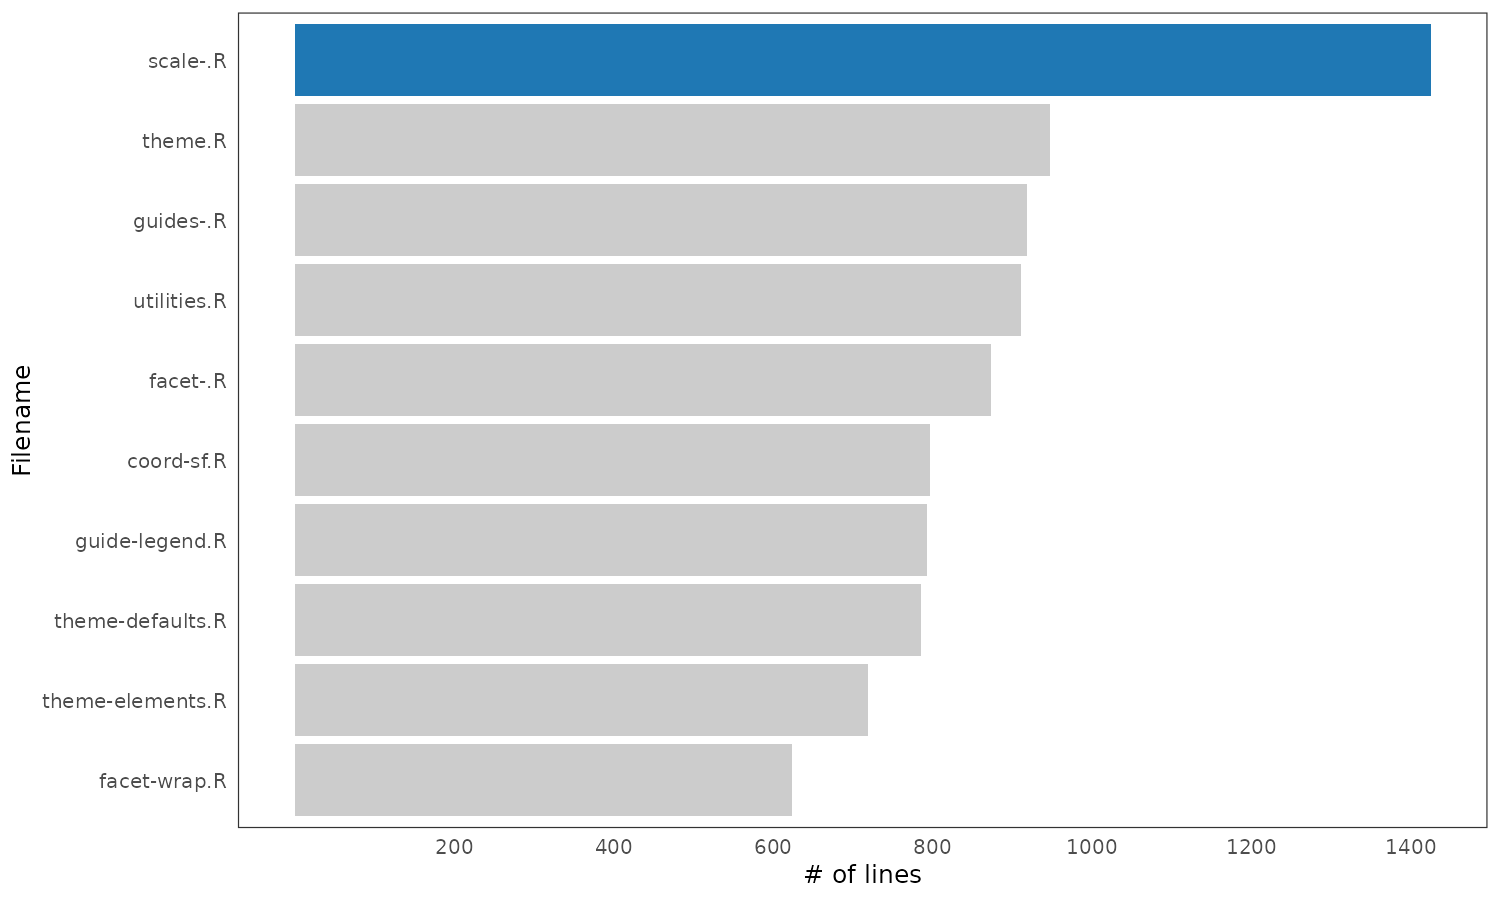
\includegraphics[width=1\linewidth,height=1\textheight]{./figures/ggplot2-linecounts} 

}

\caption{The top 10 longest source files within the `ggplot2` codebase. Notice that `scale-.R` files contains significantly more lines than the other files.}\label{fig:ggplot2-linecounts}
\end{figure}

For the reasons outlined above, I believe it is important to discuss the issue of applied scaling in more depth. The information here is based largely on how scales have been implemented in existing data visualization codebases, such as the \texttt{ggplot2}package (\citeproc{ref-wickham2016}{Wickham 2016}) or \texttt{d3-scale} module of D3 (\citeproc{ref-d3-scale2024}{Observable 2024}; used also by e.g.~Vega \citeproc{ref-satyanarayan2015}{Satyanarayan et al. 2015}), as well as on personal insights gained while implementing my package.

\subsubsection{Scales as functions}\label{scales-as-functions}

From a high-level perspective, a scale is just a function \(s: D \to V\) which maps data values \(d \in D\) to values of some visual attribute \(v \in V\), such as the x- and y-position, length, area, radius, or color (\citeproc{ref-wilkinson2012}{Wilkinson 2012}; \citeproc{ref-petricek2020}{Petricek 2020}). This function may or may not be invertible, such that, at times, each value of the visual attribute may be uniquely identifiable with a single data value, or not.

One of the most common examples of a scale is a function where both \(D\) and \(V\) are subsets of the real numbers:

\[s: [d_{min}, d_{max}] \to [v_{min}, v_{max}] \qquad d_{min}, d_{max}, v_{min}, v_{max} \in \mathbb{R}\]

For example, suppose our data takes values in the range from 1 to 10 and we want to plot it along the x-axis, within a 800 pixels wide plotting region. Then, our scale is simply:

\[s_x: [1, 10] \to [0, 800]\]

Now, there is an infinite number of functions that fit this signature. However, one particularly nice and simple candidate is the following function:

\begin{definition}[Simple linear mapping]
\protect\hypertarget{def:linear-mapping}{}\label{def:linear-mapping}\[s(d) = v_{min} + \frac{d - d_{min}}{d_{max} - d_{min}} \cdot (v_{max} - v_{min})\]
\end{definition}

if we substitute our concrete values into the formula, this becomes:

\[s_x(d) = 0 + \frac{d - 1}{10 - 1} \cdot (800 - 0) = [(d - 1) / 9] \cdot 800\]

The function acts on the data in the following way:

\begin{itemize}
\tightlist
\item
  \(s_x(1) = (1 - 1) / 9 \cdot 800 = 0\)
\item
  \(s_x(10) = (10 - 1) / 9 \cdot 800 = 800\)
\item
  \(s_x(d) \in [0, 800]\) for any \(d \in [1, 10]\)
\end{itemize}

That is, the function maps the data value 1 to pixel 0 (left border of the plotting region), value 10 to to pixel 800 (right border of the plotting region), and any value in between 1 and 10 inside the interval 0 to 800, proportionally to where in the data range it is located.

\subsubsection{Limits of modeling scales with simple functions}\label{simple-scale-limits}

Simple linear maps like the one above can work fine for basic data visualization systems. However, once we begin to add more features, this design can become prohibitive. Consider, for example, what happens if we want to:

\begin{itemize}
\tightlist
\item
  Expand the scale limits
\item
  Scale discrete data
\item
  Apply non-linear transformations
\item
  Pan, zoom, reverse, reorder, or otherwise modify the scale interactively
\end{itemize}

Having a single function with hard-coded values makes these operations difficult. Let's take the first point in the list above as a motivating example. Consider what happens to data points at the limits of the data range under the simple linear mapping:

\begin{Shaded}
\begin{Highlighting}[]
\FunctionTok{set.seed}\NormalTok{(}\DecValTok{123456}\NormalTok{)}
\NormalTok{x }\OtherTok{\textless{}{-}} \DecValTok{1}\SpecialCharTok{:}\DecValTok{10}
\NormalTok{y }\OtherTok{\textless{}{-}} \FunctionTok{rnorm}\NormalTok{(}\DecValTok{10}\NormalTok{, }\DecValTok{0}\NormalTok{, }\DecValTok{5}\NormalTok{)}
\NormalTok{col }\OtherTok{\textless{}{-}} \FunctionTok{ifelse}\NormalTok{(}\DecValTok{1}\SpecialCharTok{:}\DecValTok{10} \SpecialCharTok{\%in\%} \FunctionTok{c}\NormalTok{(}\DecValTok{1}\NormalTok{, }\DecValTok{10}\NormalTok{), }\StringTok{"indianred"}\NormalTok{, }\StringTok{"grey80"}\NormalTok{)}

\CommentTok{\# xaxs = "i" makes sure the x{-}axis limits match the data range exactly}
\FunctionTok{plot}\NormalTok{(x, y, }\AttributeTok{col =}\NormalTok{ col, }\AttributeTok{cex =} \DecValTok{3}\NormalTok{, }\AttributeTok{xaxs =} \StringTok{"i"}\NormalTok{, }\AttributeTok{pch =} \DecValTok{19}\NormalTok{)}
\end{Highlighting}
\end{Shaded}

\begin{center}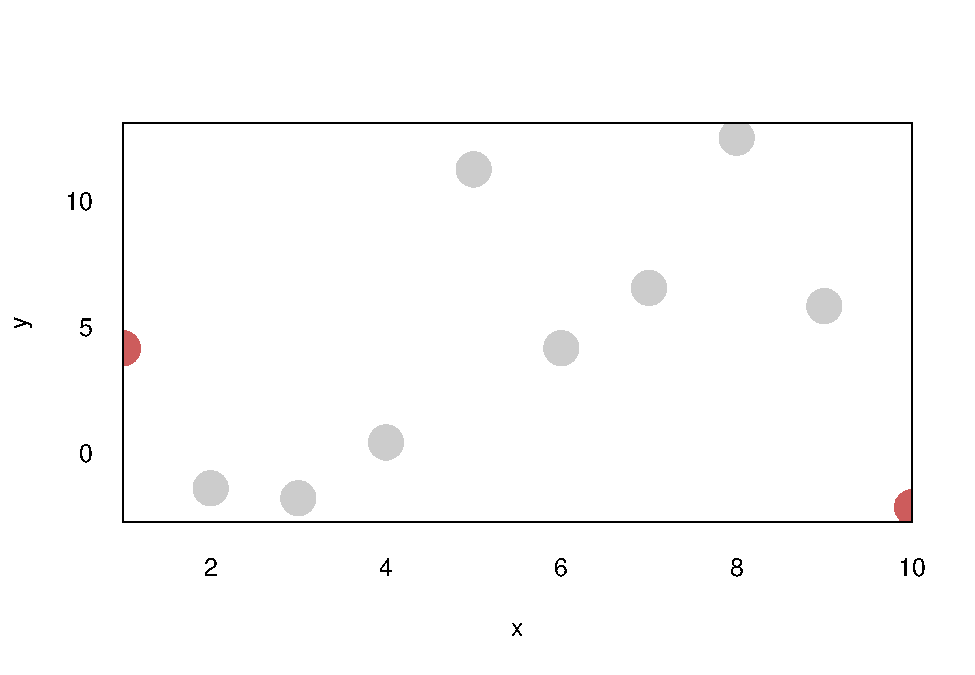
\includegraphics[width=800px,height=1\textheight]{_main_files/figure-latex/unnamed-chunk-34-1} \end{center}

The plot above shows values scaled using the simple linear mapping along the x-axis, that is, \(s: [1, 10] \to [0, 800]\) (effect of the \texttt{xaxs\ =\ "i"} argument). Notice that, since the positions of the points representing the values 1 and 10 (highlighted in red) get mapped to pixel values 0 and 800 (the left and right border of the plot), only half of each point is visible. This is problematic: as was discussed in Section \ref{show-all-data}, a fundamental principles of graphical integrity is that our graphics should not downplay or hide certain features of the data (\citeproc{ref-tufte2001}{Tufte 2001}). Since the points near the axis limits are represented by only 1/2 of the area, they become less visually salient, and this is particularly problematic since these points are more likely to be outliers.

To address this problem, most data visualization systems automatically expand the range of the domain by some pre-specified percentage:

\begin{Shaded}
\begin{Highlighting}[]
\CommentTok{\# By default, the base R plot() function automatically expands the x{-} and y{-}axis}
\CommentTok{\# limits by approximately 4\% on each end, see \textasciigrave{}xaxs\textasciigrave{} in ?graphics::par}
\FunctionTok{plot}\NormalTok{(x, y, }\AttributeTok{col =}\NormalTok{ col, }\AttributeTok{cex =} \DecValTok{3}\NormalTok{, }\AttributeTok{pch =} \DecValTok{19}\NormalTok{)}
\end{Highlighting}
\end{Shaded}

\begin{center}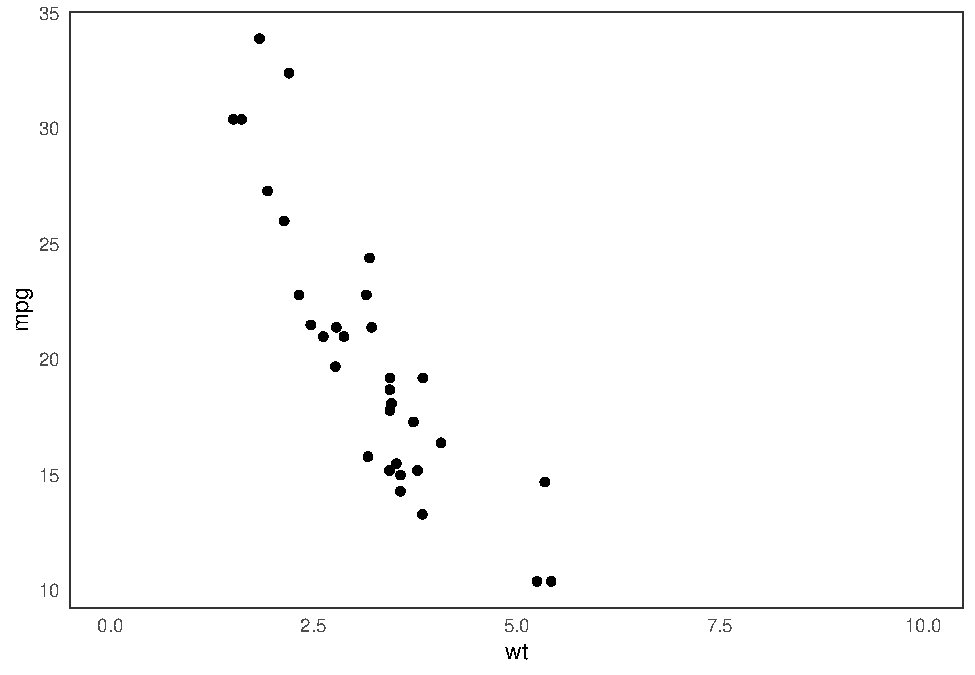
\includegraphics[width=800px,height=1\textheight]{_main_files/figure-latex/unnamed-chunk-35-1} \end{center}

We could achieve this by expanding our data range by some hard-coded percentage, for example, a symmetric 10\% margin on each side:

\begin{equation}

  s(d) = v_{min} + \bigg[ 0.1 + \frac{d - d_{min}}{d_{max} - d_{min}} \cdot (0.9 - 0.1) 
            \bigg] \cdot (v_{max} - v_{min}) 
  \label{eq:margins}

\end{equation}

However, this design becomes prohibitive as more features are added. For example, if we want to map some discrete data values to the same visual attribute codomain \(V\), do we have to design an entirely new mapping function? Similarly, what if we want to apply a different margin on each side, shift both margins by an equal amount, or flip the scale's direction? It would be useful if there were some way to abstract out the data domain \(D\) and the visual attribute \(V\), such that we could apply some common operations to the scale regardless of its specific implementation.

\subsubsection{Solution: Scales as function composition}\label{scales-composition}

The linear mapping formula in Equation \eqref{eq:margins} can guide us in decomposing the scale function into smaller, more manageable parts. Let's look at it again:

\[  s(d) = v_{min} + \bigg[ 0.1 + \frac{d - d_{min}}{d_{max} - d_{min}} \cdot (0.9 - 0.1) 
            \bigg] \cdot (v_{max} - v_{min}) \]

If we look closely, we may be able to see that the function can be split into three parts:

\begin{equation}

s(d) = \color{steelblue}{v_{min} +} \bigg[ \color{seagreen}{0.1 +} \color{indianred}{\frac{\color{black}{d} - d_{min}}{d_{max} - d_{min}}} \color{seagreen}{\cdot (0.9 - 0.1)} \bigg] \color{steelblue}{\cdot (v_{max} - v_{min})}
  
\label{eq:scale-composition}

\end{equation}

That is, the linear mapping can be interpreted as a composition of three simpler functions:

\begin{itemize}
\tightlist
\item
  \(\color{indianred}{n_D(d) = (d - d_{min}) / (d_{max} - d_{min})}\) takes a data value \(d \in D\) and maps it to the interval \([0, 1]\)\footnote{More on this below.}
\item
  \(\color{seagreen}{r(p) = 0.1 + p \cdot (0.9 - 0.1)}\) takes a value in \([0, 1]\) and maps it elsewhere in \([0, 1]\)
\item
  \(\color{steelblue}{u_V(p) = v_{min} + p \cdot (v_{max} - v_{min})}\) takes a value in \([0, 1]\) and maps it to a visual attribute value \(v \in V\)
\end{itemize}

In other words, instead of thinking of scale as mapping from \(D\) to \(V\) directly, we can break the mapping into three distinct steps. This leads us to the following definition of a scale:

\begin{definition}[Scale as function composition]
\protect\hypertarget{def:scale}{}\label{def:scale}A scale \(s: D \to V\) can be created by composing:

\begin{itemize}
\tightlist
\item
  A \emph{data normalizing} function \(n_D: D \to \mathbb{R}\), mapping data values to the real numbers \(\mathbb{R}\)
\item
  A linear \emph{rescale} function \(r: \mathbb{R} \to \mathbb{R}\)
\item
  An \emph{visual attribute unnormalizing} function \(u_V: \mathbb{R} \to V\), mapping real numbers to the visual attribute codomain
\end{itemize}

Such that:

\[s(d) = u_V(r(n_D(d)))\]
\end{definition}

This is the proposed model of scales in a nutshell. However, there are several important points which bear explaining in more detail.

\paragraph{Reusability and discrete scales}\label{reusability-and-discrete-scales}

First, by expressing scales as the composition of three functions, we gain the flexibility of three adjustable components. By choosing a specific data normalizing function \(n_D\), a rescale function \(r\), or visual attribute unnormalizing function \(u_V\), we can express a wide range of scales. Further, by swapping only one or two of the components, we may be able to create entirely new scales while reusing a lot of the functionality.

For instance, take the linear mapping from Equation \eqref{eq:scale-composition}. To turn it into a discrete scale, we could simply replace the linear mapping normalize function \(n_D(d) = (d - d_{\min}) / (d_{\max} - d_{\min})\) by some discrete mapping \(n_D\):

\[s(d) = v_{min} + \bigg[ 0.1 + n_D(d) \cdot (0.9 - 0.1) \bigg] \cdot (v_{max} - v_{min})\]
For example, if our data takes on discrete values such that, e.g.~\(d \in \{ Berlin, Prague, Vienna \}\), one simple discrete mapping may be to place the discrete values at equidistant points along the \([0, 1]\) interval:

\[n_D(d) = \begin{cases} 0.25 & \text{ if } d = Berlin \\ 0.5 & \text{ if } d = Prague \\ 0.75 & \text{ if } d = Vienna  \end{cases}\]

The function will then correctly map the discrete values in \(D = \{ Berlin, Prague, Vienna \}\) to the interval given by \([v_{\min}, v_{\max}]\), with the 10\% margins. Further, we could just as easily replace the unnormalizing function \(u_V\) by some discrete mapping, provided we wanted to scale to some discrete visual attribute values (e.g.~to a discrete colour palette).

\paragraph{The intermediate interval}\label{the-intermediate-interval}

Second, note that in Definition \ref{def:scale}, the intermediate interval is identified as \(\mathbb{R}\). This is technically correct, however, note that, for data values \(d \in D\) which fall into some \emph{typical} subset (such as \([d_{\min}, d_{\max}]\) for continuous \(D\)), \(n_D\) should \emph{generally} return values in the unit interval \([0, 1]\) (and, conversely, \(u_V\) should map values in \([0, 1]\) to typical values of the visual attribute).

The reason why the intermediate interval is identified as \(\mathbb{R}\) instead of \([0, 1]\) is because, at times, we may want to be able to map values which fall outside of the typical range of the data or the visual attribute. For instance, suppose we zoom into a region of a scatterplot and there is a point with its center just outside of the new plot limits. If the point's radius is greater than the distance of its center to the plot border, a part of the point will still overlap the plotting region and we should render it, even though the x- and y- coordinates lie outside the data range.

However, for most intents and purposes, we can act as if the intermediate interval was \([0, 1]\). This is somewhat arbitrary - any interval \([a, b]\) with \(a, b \in \mathbb{R}\) will work - however, \([0, 1]\) offers a convenient interpretation. Specifically, values \(p \in [0, 1]\) can be interpreted as percentages: for example, \(n_D(d) = 0.5\) indicates data value is at the 50th percentile of the data range, and should, therefore, be generally mapped to the middle of the visual attribute range (other factors that we will discuss later aside). Values outside of \([0, 1]\) represent data values extending beyond the data (visual attribute) range. For example, \(n_D(d) = 1.2\) suggests that the data point lies 20\% beyond the upper limit of the data range (provided that \(D\) is continuous).

Finally, note that the terms \emph{normalizing} and \emph{unnormalizing} are also arbitrary, however, I believe they make for useful labels. We can interpret them as 1D equivalent of vector normalization, mapping a one-dimensional vector in \(D\) to and from the extended unit interval \([0, 1]\) (and vice-versa for \(V\)).

\paragraph{Implementing scale features via the intermediate interval}\label{implementing-scale-features-via-the-intermediate-interval}

The three-component scale model becomes particularly useful when implementing many of the standard features of scales. Specifically, plot margins, as well as interactive features such as zooming and panning, can be implemented by manipulating the parameters of the rescale function \(r\) only. This is advantageous for reuse, since these operations can apply homomorphically, independent of the data domain \(D\) or the visual attribute codomain \(V\).

\subparagraph{Margins}\label{margins}

One feature we have seen already implemented via the rescale function are plot margins. For example, suppose we want to implement margins on the x-axis scale. Starting with a simple ``identity'' rescale function:

\[r(p) = p\]

we can shift data values closer to the centre of visual attribute range by introducing ``limits'' into the rescale function. For example, to implement symmetric 10\% margins on each side, we can rescale with \((0.1, 0.9)\) limits:

\[r(p) = 0.1 + p \cdot (0.9 - 0.1)\]

However, the limits do not have to be symmetric. For example, we could implement a 10\% left margin and 30\% right margin like so:

\[r(p) = 0.1 + p \cdot (0.7 - 0.1)\]

Importantly, the margins are independent of the data domain \(D\) and the visual attribute codomain \(V\). As long as the data normalizing function correctly maps values \(D \to \mathbb{R}\) and the visual attribute unnormalizing function correctly maps values \(\mathbb{R} \to V\), the scale will correctly implement margins.

\subparagraph{Panning}\label{panning}

Now, suppose we also want to pan the plot 25\% to the right. Again, all we need to do is to change the parameters of the rescale function for the x-axis scale. For example, using the scale with 10\% symmetric margins above, we can simply increment the scale limits by 0.25:

\begin{align}

r(p) &= (0.1 + 0.25) + p \cdot [(0.9 + 0.25) - (0.1 + 0.25)] \\
    &= 0.35 + p \cdot (1.15 - 0.35)

\end{align}

Now, the ``least'' data point \(d \in D\) will get mapped to 0.35 (10\% margin + 25\% to the right), whereas the ``greatest'' data point will get mapped to 1.15 (25\% to the right - 10\% margin). Notice that, again, this is entirely independent of \(D\) and \(V\). That is, for instance, we can pan a continuous scale the exact same way we can pan a discrete scale.

\subparagraph{Zooming}\label{zooming}

Zooming can also be implemented entirely using the rescale function \(r\). The key here is to notice that if we set the limits outside of \([0, 1]\), the scale essentially gets stretched such that the least and the greatest data values get mapped outside of the visual attribute range (leading to a zoom behavior).

For instance, setting the limits to \(-(0.5, 1.5)\) effectively zooms into the middle 50\% of the range, since the 25th percentile data value gets mapped to zero and the 75th percentile data value gets mapped to one:

\[r(0.25) = -0.5 + 0.25 \cdot [1.5 - (-0.5)] = 0\]
\[r(0.75) = -0.5 + 0.75 \cdot [1.5 - (-0.5)] = 1\]

Care must be taken when zooming in the presence of pre-existing limits, such as those caused by margins or multiple levels of zoom. In that case, we need to re-normalize the new limits within the context of the current limits. Coming up with the right formula requires a bit of careful algebra; details of the algorithm are given in Section \ref{scales}.

\paragraph{Inverses}\label{inverses}

Another advantage of the three component scale system is that if both \(n_D\) and \(u_V\) have inverses (or at least retractions), we can easily implement an inverse scale function. Specifically, let \((n_D)^{-1} = u_D\) and \((u_V)^{-1} = n_V\) such that \(u_D: \mathbb{R} \to D\) and \(n_V = V \to \mathbb{R}\), and \(u_D \circ n_D = n_V \circ u_V = \text{id}\), the identity function. Then:

\[s^{-1}(v) = u_D(r^{-1}(n_V(v)))\]

(the inverse of the rescale function \(r\), \(r^{-1}\), effectively always exists, since the function is just a simple linear map)

The inverse scale function allows us to go from the values of the visual attribute to the values of the data domain. This may be useful in certain situations, such as when we want to find the closest data point to a given x- and y-axis coordinate.

However, as was mentioned above, \(n_D\) and \(u_V\) may not always have a full inverse. For example, such is the case with the discrete mapping \(n_D\):

\[n_D(d) = \begin{cases} 0.25 & \text{ if } d = Berlin \\ 0.5 & \text{ if } d = Prague \\ 0.75 & \text{ if } d = Vienna  \end{cases}\]
We can construct a function which reverts the effect of \(n_D\):

\[u_D(p)^ = \begin{cases} Berlin & \text{ if } p = 0.25 \\ Prague & \text{ if } p = 0.5 \\ Vienna & \text{ if } p = 0.75  \end{cases}\]
Such that \(u_D(n_D(d)) = d\) for all \(d \in D\). However, the converse is not necessarily true: it is not the case that \(n_D(u_D(p)) = p\) for all \(p \in \mathbb{R}\), since \(u_D(p)\) is only defined for \(p \in \{ 0.25, 0.5, 0.75 \}\). We could construct \(u_D\) in such a way that it e.g.~maps the intermediate value \(p\) to the ``closest'' value in \(D\), such that, e.g.~\(p < 0.375\) gets mapped to \(Berlin\), \(0.375 \leq p < 0.625\) gets mapped to \(Prague\), and \(p \geq 0.625\) get mapped to \(Vienna\). This way, \(u_D(p)\) will be defined for all \(p \in \mathbb{R}\), however, it is still not the case that \(n_D(u_D(p)) = p\) for all \(p \in \mathbb{R}\). And such will be the case for any finite \(D\), or more generally, any time the dimensionalities of \(D\) and \(V\) do not match. However, even when the functions have only a one-sided inverse (a retraction), the inverse scale function may still prove quite useful.

\paragraph{Scale transformations}\label{scale-transformations}

\begin{quote}
``Transformation is a critical tool for visualization or for any other mode of data analysis
because it can substantially simplify the structure of a set of data.''

Cleveland (\citeproc{ref-cleveland1993}{1993}), pp.~48
\end{quote}

\subsubsection{Comparison to past implementations of scales}\label{comparison-to-past-implementations-of-scales}

Many popular data visualization systems implement a multi-component model of scales similar to the one outlined above, however, they typically omit the \(r\) function and implement the \(n_D\) and \(u_V\) mappings quite differently. For example, in \texttt{D3} (\citeproc{ref-bostock2011}{Michael Bostock, Ogievetsky, and Heer 2011}), scales are implemented in a functional style, such that the data domain and the visual attribute codomain are passed as tuples or arrays of values to a higher-order \texttt{scale*} function (such as \texttt{scaleLinear}, \texttt{scalePoint}, or \texttt{scaleBand}), which then returns a new function that can be used for scaling. The domain and codomain can also be modified afterwards, using the \texttt{scale*.domain} and \texttt{scale*.range} methods respectively (JavaScript functions are objects and can have other functions/methods attached to them).

For illustration, here are few examples from the official documentation (\citeproc{ref-d3-scale2024}{Observable 2024}):

\begin{Shaded}
\begin{Highlighting}[]
\KeywordTok{const}\NormalTok{ x }\OperatorTok{=}\NormalTok{ d3}\OperatorTok{.}\FunctionTok{scaleLinear}\NormalTok{([}\DecValTok{10}\OperatorTok{,} \DecValTok{130}\NormalTok{]}\OperatorTok{,}\NormalTok{ [}\DecValTok{0}\OperatorTok{,} \DecValTok{960}\NormalTok{])}\OperatorTok{;}
\FunctionTok{x}\NormalTok{(}\DecValTok{20}\NormalTok{)}\OperatorTok{;} \CommentTok{// 80}
\KeywordTok{const}\NormalTok{ color }\OperatorTok{=}\NormalTok{ d3}\OperatorTok{.}\FunctionTok{scaleLinear}\NormalTok{([}\DecValTok{10}\OperatorTok{,} \DecValTok{100}\NormalTok{]}\OperatorTok{,}\NormalTok{ [}\StringTok{"brown"}\OperatorTok{,} \StringTok{"steelblue"}\NormalTok{])}\OperatorTok{;}
\FunctionTok{color}\NormalTok{(}\DecValTok{20}\NormalTok{)}\OperatorTok{;} \CommentTok{// "rgb(154, 52, 57)"}
\CommentTok{// The domain and codomain can be changed after initialization}
\KeywordTok{const}\NormalTok{ y }\OperatorTok{=}\NormalTok{ d3}\OperatorTok{.}\FunctionTok{scaleLinear}\NormalTok{()}\OperatorTok{.}\FunctionTok{domain}\NormalTok{([}\DecValTok{10}\OperatorTok{,} \DecValTok{130}\NormalTok{])}\OperatorTok{;} 
\end{Highlighting}
\end{Shaded}

Internally, the \texttt{scale*} functions rely on other specialized functions to translate from its domain to the codomain (such as the \texttt{normalize()} and \texttt{scale()} functions for continuous and discrete/ordinal domains, respectively, and various \texttt{interpolate()} functions for codomains).

Similarly, in \texttt{ggplot2} (\citeproc{ref-wickham2016}{Wickham 2016}), all scales inherit from the \texttt{Scale} base class, with each subtype implementing \texttt{limits} and \texttt{palette} properties. The \texttt{limits} property is a vector which corresponds to the data domain and the \texttt{palette} property is a function which corresponds roughly to the visual codomain (the x- and y-position behave slightly differently, due to being transformed via coordinate systems). Internally, the package uses the \texttt{rescale} function from the \texttt{scales} package (\citeproc{ref-wickham2023}{Wickham, Pedersen, and Seidel 2023}) to map data values to \([0, 1]\) and then the \texttt{palette} function is responsible for mapping these normalized values to the visual attribute. For illustration, here's the full definition of the \texttt{map} method on the \texttt{ScaleContinuous} class (I've added comments for clarity):

\begin{Shaded}
\begin{Highlighting}[]
\NormalTok{map }\OtherTok{=} \ControlFlowTok{function}\NormalTok{(self, x, }\AttributeTok{limits =}\NormalTok{ self}\SpecialCharTok{$}\FunctionTok{get\_limits}\NormalTok{()) \{}
  \CommentTok{\# Limits are just a tuple, rescale maps x to [0, 1]}
\NormalTok{  x }\OtherTok{\textless{}{-}}\NormalTok{ self}\SpecialCharTok{$}\FunctionTok{rescale}\NormalTok{(self}\SpecialCharTok{$}\FunctionTok{oob}\NormalTok{(x, }\AttributeTok{range =}\NormalTok{ limits), limits) }

\NormalTok{  uniq }\OtherTok{\textless{}{-}} \FunctionTok{unique0}\NormalTok{(x)}
  \CommentTok{\# Palette is a function which returns a vector of attribute values}
\NormalTok{  pal }\OtherTok{\textless{}{-}}\NormalTok{ self}\SpecialCharTok{$}\FunctionTok{palette}\NormalTok{(uniq) }
\NormalTok{  scaled }\OtherTok{\textless{}{-}}\NormalTok{ pal[}\FunctionTok{match}\NormalTok{(x, uniq)]}

  \FunctionTok{ifelse}\NormalTok{(}\SpecialCharTok{!}\FunctionTok{is.na}\NormalTok{(scaled), scaled, self}\SpecialCharTok{$}\NormalTok{na.value)}
\NormalTok{\}}
\end{Highlighting}
\end{Shaded}

Thus, a key difference between the models of scales discussed above, and the model I propose, is that the domain and codomain are generally implemented as different types. In \texttt{D3}, internally, the functions used to translate from \(D \to \mathbb{R}\) are fundamentally different from those used to translate from \(\mathbb{R} \to V\). This difference is even more pronounced in \texttt{ggplot2}, where \texttt{limits} is a simple vector/tuple whereas \texttt{palette} is a function.

I contend that having different types for the domain and codomain has several disadvantages. First, it impedes code reuse, since we cannot simply use the same object in either place. Second, it complicates the mental model: the user has to hold a completely different concept for the domain and codomain in their head. Finally, the models of scales outlined above are designed to work in only one direction: from the data to the visual attribute. To go the other way around, from the visual attribute to the data, other, specialized functions have to be implemented.

Instead, I propose a unified model where the data domain and visual attribute codomain differ only in the context they are used. Details will be discussed in Section \ref{scales}.

\section{Rendering}\label{rendering}

\chapter{Goals}\label{goals}

The primary aim of this doctoral project was to develop an original interactive data visualization system, while attempting to provide solutions to the problems described in Section \ref{problems}. This was realized through the creation and publication of the R package \texttt{plotscaper} (available on \href{https://cran.r-project.org/web/packages/plotscaper/index.html}{CRAN}) and the underlying JavaScript package \texttt{plotscape} (available on \href{https://www.npmjs.com/package/@abartonicek/plotscape}{NPM}). This section outlines some general concerns that informed the more specific design decisions that will be discussed in Section \ref{system}.

\section{User profile}\label{user-profile}

A key first step in designing any kind of system is understanding the target audience. This is especially the case in interactive data visualization systems, which cater to a diverse range of users. As was discussed in Section \ref{litreview}, users of interactive data visualization systems can differ in their analysis goals, experience, and motivation. At one end of the spectrum, some interactive data visualization systems are designed with fairly minimal expectations of the user's level of experience or motivation. Conversely, other systems assume a highly motivated ``expert'' users with a sufficient level of domain expertise (\citeproc{ref-dimara2019}{Dimara and Perin 2019}) or the ability to contend with low-level execution details such as rendering or reactive event graph (\citeproc{ref-satyanarayan2015}{Satyanarayan et al. 2015}, \citeproc{ref-satyanarayan2016}{2016}).

The goal was to design a package for interactive data exploration that would be accessible to a wide range of R users. Specifically, I wanted to enable even the novice users to quickly create comprehensive interactive figures they could use to explore their data, while, at the same time, allowing more advanced users to take advantage of the full range of features and engage in deeper customization. This necessitated a generally simple design, with low-level implementation details abstracted away. Consequently, the design prioritized several key features: a simple API with sensible defaults, a clean and intuitive user interface, and a robust set of built-in interactive capabilities.

\section{Programming interface}\label{programming-interface}

To make the package accessible to a wide range of R users, a key concern was designing a simple and intuitive application programming interface (\hyperref[API]{API}). Specifically, I wanted to make it easy for the average user to learn the package and produce fairly complete and useful interactive figures, with only few lines of R code. Ideally, the package should empower even users with limited programming experience to take advantage of interactive graphics.

Achieving this level of accessibility required several design choices. First, the API had to be easy to learn. I tried to accomplish this by drawing inspiration from established packages. Specifically, the main inspirations for the \texttt{plotscaper} API were the popular \texttt{ggplot2} package (\citeproc{ref-wickham2016}{Wickham 2016}), as well as the \texttt{iplots} package (\citeproc{ref-urbanek2003}{Urbanek and Theus 2003}; \citeproc{ref-urbanek2011}{Urbanek 2011}). However, \texttt{plotscaper}`s design goals also necessitated some deviations from these packages' APIs, see Section \ref{system}. Second, to further simplify the API, many of the components such as scales had to be given sensible defaults. Conversely, this also meant that extensive customizability was not a primary concern: the goal was to empower the users to start exploring their data quickly, rather than spend time making fine-grained adjustments to their figures. Third, to broaden its appeal, the package had to integrate seamlessly with existing tools within the R ecosystem. These included the popular RStudio \hyperref[ide]{IDE} (\citeproc{ref-rstudio2024}{Posit 2024}) and the RMarkdown document-authoring system (\citeproc{ref-xie2018}{Xie, Allaire, and Grolemund 2018}).

\section{User interface}\label{user-interface}

While ease of writing user code was a key consideration, equally important was the ease of interpreting and interacting with the resulting visualizations. The visual design of the figures needed to promote acquisition of statistical insights, and the figures' interactive behavior had to be clear and intuitive. As was discussed in Section \ref{litreview}, effective visual design is of key impoertance, as poor design can make figures less legible or even misleading (see e.g. \citeproc{ref-tufte2001}{Tufte 2001}; \citeproc{ref-cairo2014}{Cairo 2014}, \citeproc{ref-cairo2019}{2019}; \citeproc{ref-franconeri2021}{Franconeri et al. 2021}). Similarly, the design of interactions can either enhance or hinder the acquisition of insights.

A general rule I applied to the design of the user interface \texttt{plotscaper} was ``less is more''. Specifically, following Tufte's (\citeproc{ref-tufte2001}{2001}) example, I aimed to design figures that would prioritize showing the data above all else. Visually, this was achieved by minimizing auxiliary graphical elements such as axis ticks, labels, and grid lines. I also tried to strive for a minimalist ``pen and paper'' look and feel, as if the figures were drawn in a notebook. For color, I decided to use muted colors for non-data elements and an established color palette for representing the data. Finally, when it came to interactive features, I tried to approach those with similar degree of minimalism. I tried to avoid distracting interactive features, such as having query tool-tips always appear on hover by default, and in general tried to design the user interactions in a way that would complement but not overwhelm the visual experience.

\section{Interactive features}\label{interactive-features}

The next important question was which interactive features to support. As was discussed in Section \ref{litreview}, there are many interactive data visualization features, and some are more useful than others (for data exploration, anyway). Furthermore, the amount of time and effort required to implement these features also varies considerably. Therefore, choosing the right set of features to prioritize was a key design consideration.

As was hinted at throughout Section \ref{litreview}, the core feature to implement was generalized linked selection or brushing. Specifically, every plot in \texttt{plotscaper} needed to support both dispatching and displaying selection events. This feature is highly desirable because it allows users to quickly explore trends across dynamically-generated subsets of their data, making it one of the most useful tools in the interactive data visualization arsenal (\citeproc{ref-buja1996}{Buja, Cook, and Swayne 1996}; \citeproc{ref-heer2012}{Heer and Shneiderman 2012}; \citeproc{ref-wilhelm2003}{Wilhelm 2003}, \citeproc{ref-wilhelm2008}{2008}; \citeproc{ref-wills2008}{G. Wills 2008}; \citeproc{ref-ware2019}{Ware 2019}; \citeproc{ref-ward2015}{Ward, Grinstein, and Keim 2015}). However, it also requires a significant amount of careful planning and programming effort. Simply adding this functionality on top of an existing static data visualization system does not work. Naive solutions, like replacing the entire plot upon selection, produce unsatisfactory behavior, see for example the following quote by Adalbert Wilhelm from chapter II.9 of the Data Visualization Handbook:

\begin{quote}
``{[}Replacing the entire plot{]} only works fine when we have individual plot symbols for each observation, as in scatterplots for example, where some attributes are changed by the user interaction. But even when replacing plot parameters the user loses the possibility to compare the current plot with previous versions. The
user can only compare the current image with a mental copy of the previous image and hence the comparison might get distorted.''

(\citeproc{ref-wilhelm2008}{Wilhelm 2008, 210})
\end{quote}

Thus, linked selection had to be directly integrated into the data visualization pipeline, or rather, the data visualization pipeline had to be built around this feature. This was a significant programming challenge. Crucially also, I aimed for a consistent linked selection behavior across \emph{all} implemented plot types. This necessitated careful consideration of the issues discussed in Section \ref{problems}.

Other important features which also had to be directly integrated into the data visualization pipeline were parameter manipulation and representation switching. These features give the user the ability to quickly see alternative views of their data and discover trends that they may otherwise miss (see Sections \ref{changing-representation}). This makes them highly desirable.

Another interesting challenge was querying. Upon seeing an interesting visual trend in their data, users may often be interested in the precise data values that produced that visual impression. Thus, being able to interactively query geometric objects is very useful. This feature is arguably simpler to implement than the previously mentioned features, however, it should be noted that what complicates its implementation is that, often, the user does not directly care about the visual attributes of the queried geometric objects, but the instead the statistics underlying those visual attributes. For instance, when querying a stacked barplot, we do not care about the stacked values, but instead about the values corresponding to individual segments. Thus, querying provided an intermediate level of challenge.

Other interesting feature was bi-directional communication. The ability to call functions in an interactive session and have the figure respond directly can be invaluable in data exploration. However, compared to a static data visualization, this requires a specialized setup, such as having live server respond to messages from the client. Thus, developing a system for communicating between the R client and the JavaScript ``backend'' (the figure) was necessary.

Finally, there were some useful features which were relatively simple to implement. These included changing size and alpha, zooming, and panning. These features could be implemented by manipulating scales and/or the visual attributes of geometric objects, without modifying earlier stages of the data visualization pipeline. Nevertheless, desppite their simplicity, these features could still be highly useful. For example, zooming and panning can help to reveal trends within narrow data ranges, while adjustments to size and alpha can mitigate overplotting. Therefore, implementing these features was an easy choice.

Some features I did not choose to implement were complex logical selection, semantic zooming, and {[}LIST OTHERS{]}. Logical selection refers to the ability of being able to use logical operators such as AND, OR, and XOR with selection events to create more complex selections (see e.g. \citeproc{ref-theus2008}{Theus 2008}). While this feature can be undeniably a powerful tool in the hands of more advanced users, its utility for novices is debatable. G. J. Wills (\citeproc{ref-wills2000}{2000}) argued that selection systems should be simple, powerful, and forgiving, and as such, I did not choose to prioritize complex selection operators, opting instead for simple transient/persistent selection. More sophisticated selection operators could also always be implemented later. As for semantic zooming, I did not choose to prioritize this feature since, while also undeniably useful in certain situations, it is fairly complex and applies only to a limited set of plot types such as maps. Generally, I focused on features that could apply across many different plot types, and this gave features like semantic zooming lower priority.

\chapter{High-level design}\label{high-level-design}

\begin{quote}
``Designing is fundamentally about taking things apart {[}\ldots{]} in such a way that they can be put back together. Separating things into things that can be composed.''

Rich Hickey (\citeproc{ref-hickey2013}{2013})
\end{quote}

This section contains a description of some of the high-level design decisions that went into making the system.

\begin{quote}
The example code chunks in this section are written in both R and TypeScript. While I would prefer to use R for all code examples, due to its tight integration with RMarkdown, some of the concepts are much easier to explain in a language with static typing like TypeScript (particularly, type annotations and interfaces). However, since some examples can also be greatly enhanced by graphical output, I also wanted to use R.

So, where graphical output is important, the code examples are written in R, and, where the code itself is the main focus, they are written in TypeScript. I hope this bilingualism is not too confusing. I have tried to use only the core features of each language to make the examples clear.
\end{quote}

\subsection{User profile}\label{user-profile-1}

When designing an interactive data visualization system, one important consideration is the profile of the average user. Among interactive data visualization systems, there can be significant differences in what the user is expected to know, across various implementations and research areas. For example, some general interactive data visualization systems make almost no assumptions about the user's level of experience or motivation, whereas others assume a highly motivated ``expert'' user with a sufficient level of domain knowledge (\citeproc{ref-dimara2019}{Dimara and Perin 2019}).

The goal of the project was to design a fairly versatile system for general data exploration. As such, the system was designed in such a way to make it possible for someone with fairly modest data science skills to pick up and make decent use of its basic features. At the same time, I also wanted to provide some more advanced features that experienced users could make use of.

{[}Give examples{]}.

\section{Programming paradigm}\label{programming-paradigm}

\begin{quote}
``Apex predator of Grug is complexity. Complexity bad. Say again: complexity very bad.
You say now: complexity very, very bad. Given choice between complexity or one on one
against T-rex, Grug take T-rex: at least grug see T-rex.''

The Grug Brained Developer, Gross (\citeproc{ref-gross2024}{2024})
\end{quote}

It is often the case that single programming task can often be solved in many different ways, each with its own set of trade-offs. These trade-offs affect factors like performance, readability, reliability, and maintainability. With regards to these trade-offs, one of the most fundamental decisions is the choice of a programming paradigm.

Programming paradigms provide a set of high-level guidelines for thinking about and solving programming problems. They offer distinct approaches to issues such as data representation, code organization, and control flow. Underlying these are philosophical differences on topics such as data mutability, the fundamental unit of computation. These differences can produce programs of radically different shapes and styles.

However, all programming paradigms ultimately share one fundamental concern: complexity (\citeproc{ref-booch2008}{Booch et al. 2008}). Every programming problem comes with some inherent level of complexity. Without careful thought and constant effort, software has the tendency to grow out of scope and becomes unmanageable (\citeproc{ref-moseley2006}{Moseley and Marks 2006}). Thus, all programming paradigms provide answers to the fundamental problem of complexity, each in their own idiosyncratic way (\citeproc{ref-chambers2014}{Chambers 2014}; \citeproc{ref-jordan2015}{Jordan et al. 2015}; \citeproc{ref-moseley2006}{Moseley and Marks 2006}; \citeproc{ref-van2009}{Van Roy et al. 2009}).

Most programming languages are geared towards one specific programming paradigm, and typically support only one or two to a reasonable capacity (\citeproc{ref-van2009}{Van Roy et al. 2009}). Fortunately, this is not the case for either JavaScript/TypeScript or R, since both are multiparadigm programming languages (\citeproc{ref-chambers2014}{Chambers 2014}; \citeproc{ref-mdn2024c}{MDN 2024f}). Both languages support object-oriented programming, via prototype inheritance in the case of JavaScript (\citeproc{ref-mdn2024d}{MDN 2024b}) and the S3, S4, and R6 systems in the case of R (\citeproc{ref-wickham2019}{Wickham 2019}), and treat functions as first class citizens, allowing for functional programming style (\citeproc{ref-chambers2014}{Chambers 2014}; \citeproc{ref-mdn2024e}{MDN 2024d}). Further, as C based languages, both also support classical imperative/procedural programming style, and also provide some utilities for reflective metaprogramming.

The flexibility of JavaScript and R had allowed me to experiment with different programming paradigms while developing my interactive data visualization package. I have rewritten the JavaScript side of the package multiple times from scratch, testing out several different programming paradigms and styles in the process. Below, I provide a rough sketch of the paradigms I have sampled, as well as an account of my experience of using each paradigm and some thoughts on its suitability for designing interactive data visualization systems.

\subsection{Imperative programming}\label{imperative-programming}

Imperative programming is one of the oldest and most classical programming paradigms. It conceptualizes the program as a sequence of discrete steps that manipulate some mutable state (\citeproc{ref-frame2014}{Frame and Coffey 2014}). In this way, it closely resembles the way computer programs get executed on the underlying hardware (barring some advanced techniques such as branch prediction and speculative execution, the CPU executes instructions sequentially, see e.g. \citeproc{ref-parihar2015}{Parihar 2015}; \citeproc{ref-raghavan1998}{Raghavan, Shachnai, and Yaniv 1998}).

\subsection{Functional programming}\label{functional-programming}

\subsection{Object oriented programming}\label{object-oriented-programming}

Object oriented programming (OOP) is a widely used programming paradigm. It first appeared in the late 1950's and early 1960's, with languages like Simula and Smalltalk (\citeproc{ref-black2013}{Black 2013}). It then grew to prominence in the 1980's and 1990's, eventually becoming an industry standard.

While there are may different interpretations of OOP, there are several concepts which tend to be shared by most implementations. The core idea of OOP is that programs should be modeled as networks of objects: independent units of computation which bundle related data (properties, members) and code (methods, virtual functions) together (\citeproc{ref-booch2008}{Booch et al. 2008}). Objects are self-contained, and own hidden, private state; they expose only a limited public interface. To communicate with each other, objects send each other messages (\citeproc{ref-meyer1997}{Meyer 1997}). In this way, they behave similarly to networks of biological cells (this was the inspiration for Alan Kay, one of the creators of Smalltalk, who also coined the term ``object oriented,'' \citeproc{ref-kay1996}{Kay 1996}).

Each object is instantiated based on a class, a sort of a blueprint which provides the object with a type as well as implementation of its methods. Classes can be associated with each other in various ways. For example, a class may inherit methods and properties from a parent class (superclass), such that it can make use of the parent's implementation. Alternatively, a class may be composed of other classes, by having their instances as properties.

Here's a basic example one might see in an introductory OOP text-book (for some reasons, animals are a popular metaphor in introductory OOP texts). We start with a base class \texttt{Animal}:

\begin{Shaded}
\begin{Highlighting}[]
\CommentTok{// Animal.ts}
\KeywordTok{type}\NormalTok{ Food }\OperatorTok{=}\NormalTok{ \{ nutrition}\OperatorTok{:} \DataTypeTok{number}\NormalTok{ \}}\OperatorTok{;}

\ImportTok{export} \KeywordTok{class}\NormalTok{ Animal \{}
  \CommentTok{// Class properties with default values}
\NormalTok{  x }\OperatorTok{=} \DecValTok{0}\OperatorTok{;} 
\NormalTok{  y }\OperatorTok{=} \DecValTok{0}\OperatorTok{;}
\NormalTok{  nutrition }\OperatorTok{=} \DecValTok{100}\OperatorTok{;}

  \CommentTok{// A basic method shared by all Animals}
  \FunctionTok{move}\NormalTok{(dx}\OperatorTok{:} \DataTypeTok{number}\OperatorTok{,}\NormalTok{ dy}\OperatorTok{:} \DataTypeTok{number}\NormalTok{) \{}
    \KeywordTok{this}\OperatorTok{.}\AttributeTok{x} \OperatorTok{+=}\NormalTok{ dx}\OperatorTok{;}
    \KeywordTok{this}\OperatorTok{.}\AttributeTok{y} \OperatorTok{+=}\NormalTok{ dy}\OperatorTok{;}
\NormalTok{  \}}

  \CommentTok{// Default eat method}
  \FunctionTok{eat}\NormalTok{(food}\OperatorTok{:}\NormalTok{ Food) \{}
    \KeywordTok{this}\OperatorTok{.}\AttributeTok{nutrition} \OperatorTok{+=}\NormalTok{ food}\OperatorTok{.}\AttributeTok{nutrition}\OperatorTok{;}
\NormalTok{  \}}
\NormalTok{\}}
\end{Highlighting}
\end{Shaded}

Next, we subclass the \texttt{Animal} class and create a \texttt{Dog} class:

\begin{Shaded}
\begin{Highlighting}[]
\ImportTok{import}\NormalTok{ \{ Animal \} }\ImportTok{from} \StringTok{"./Animal.ts"}

\KeywordTok{type}\NormalTok{ Meat }\OperatorTok{=}\NormalTok{ \{ type}\OperatorTok{:} \VerbatimStringTok{\textasciigrave{}meat\textasciigrave{}}\OperatorTok{;}\NormalTok{ nutrition}\OperatorTok{:} \DataTypeTok{number}\NormalTok{ \}}\OperatorTok{;}

\KeywordTok{class}\NormalTok{ Dog }\KeywordTok{extends}\NormalTok{ Animal \{}
  \CommentTok{// Overwrite superclass method {-} dogs only eat meat}
  \FunctionTok{eat}\NormalTok{(food}\OperatorTok{:}\NormalTok{ Meat) \{ }
    \KeywordTok{super}\OperatorTok{.}\FunctionTok{eat}\NormalTok{(food)}\OperatorTok{;} \CommentTok{// Call superclass method}
\NormalTok{  \}}

  \CommentTok{// Dogs also makes a specific dog{-}like sound}
  \FunctionTok{getSound}\NormalTok{() \{ }
    \ControlFlowTok{return} \VerbatimStringTok{\textasciigrave{}Woof!\textasciigrave{}}\OperatorTok{;}
\NormalTok{  \}}
\NormalTok{\}}

\KeywordTok{const}\NormalTok{ dog }\OperatorTok{=} \KeywordTok{new} \FunctionTok{Dog}\NormalTok{()}\OperatorTok{;}

\CommentTok{// Dog inherits all of the methods and properties of Animal}
\NormalTok{dog}\OperatorTok{.}\FunctionTok{move}\NormalTok{(}\OperatorTok{{-}}\DecValTok{10}\OperatorTok{,} \DecValTok{10}\NormalTok{)}\OperatorTok{;} 
\NormalTok{dog}\OperatorTok{.}\FunctionTok{eat}\NormalTok{(\{ type}\OperatorTok{:} \VerbatimStringTok{\textasciigrave{}meat\textasciigrave{}}\OperatorTok{,}\NormalTok{ nutrition}\OperatorTok{:} \DecValTok{10}\NormalTok{ \})}\OperatorTok{;} \CommentTok{// This is fine}
\CommentTok{// dog.eat(\{ type: \textasciigrave{}vegatable\textasciigrave{}, nutrition: 10 \}); // This would result in a compiler error}

\BuiltInTok{console}\OperatorTok{.}\FunctionTok{log}\NormalTok{([}\VerbatimStringTok{\textasciigrave{}x\textasciigrave{}}\OperatorTok{,} \VerbatimStringTok{\textasciigrave{}y\textasciigrave{}}\OperatorTok{,} \VerbatimStringTok{\textasciigrave{}nutrition\textasciigrave{}}\NormalTok{]}\OperatorTok{.}\FunctionTok{map}\NormalTok{(e }\KeywordTok{=\textgreater{}} \VerbatimStringTok{\textasciigrave{}}\SpecialCharTok{$\{}\NormalTok{e}\SpecialCharTok{\}}\VerbatimStringTok{: }\SpecialCharTok{$\{}\NormalTok{dog[e]}\SpecialCharTok{\}}\VerbatimStringTok{\textasciigrave{}}\NormalTok{)}\OperatorTok{.}\FunctionTok{join}\NormalTok{(}\VerbatimStringTok{\textasciigrave{}, \textasciigrave{}}\NormalTok{))}
\BuiltInTok{console}\OperatorTok{.}\FunctionTok{log}\NormalTok{(dog}\OperatorTok{.}\FunctionTok{getSound}\NormalTok{())}\OperatorTok{;}
\end{Highlighting}
\end{Shaded}

\begin{verbatim}
## x: -10, y: 10, nutrition: 110
## Woof!
\end{verbatim}

This is only a toy example of OOP code. In real applications, when writing OOP code, one may also rely on more advanced language features such as interfaces, abstract classes, and generics, however, a detailed discussion of these features is outside of the scope of the present thesis. Nevertheless, what is important to discuss are some fundamental theoretical ideas behind OOP.

\subsubsection{Abstraction}\label{abstraction}

Abstraction is a fundamental concept in OOP. It refers to the idea that, after having built a system (class) out of components (values and other classes), one should be able to ``forget'' all of the messy internal details and only rely on the exposed public interface. For instance, in the example above, the \texttt{Dog} class inherits from the \texttt{Animal} class: we should be able to use the methods inherited from \texttt{Animal} (such as \texttt{move}) without having to remember how these methods were implemented on the \texttt{Animal} class.

Ultimately, the goal of abstraction is to make it possible to reason about complex systems (\citeproc{ref-booch2008}{Booch et al. 2008}). By hiding away details, good abstractions can free us to think about higher-level concepts. Fundamentally, this also comes with a shift of perspective: instead of thinking about the data objects are composed of, we should only consider their behavior (\citeproc{ref-black2013}{Black 2013}; \citeproc{ref-meyer1997}{Meyer 1997}).

\subsubsection{Encapsulation}\label{encapsulation}

An idea closely related to abstraction is encapsulation. Encapsulation refers to the practice of controlling access to class internals. Specifically, to properly encapsulate its data, a class should expose only a limited number of properties/methods and the rest should be kept private (\citeproc{ref-booch2008}{Booch et al. 2008}). Note that this does not mean that the hidden parts of a class have to be entirely \emph{invisible} to the user, merely that the user should not be able to access the hidden data and rely on it in their applications (\citeproc{ref-meyer1997}{Meyer 1997}).

The main goal of encapsulation is continuity. By encapsulating private properties, the developer is free to modify them without affecting the public interface (\citeproc{ref-booch2008}{Booch et al. 2008}; \citeproc{ref-meyer1997}{Meyer 1997}). In other words, users can continue using the class the same way, even while the developer is actively modifying the internals.

Encapsulation is also closely related to the ideas of the \emph{open-closed} principle and \emph{small interfaces} (\citeproc{ref-meyer1997}{Meyer 1997}). The open-closed principles states that modules should be open to extension but closed to modification. The idea of small interfaces suggests that, when communicating via messages (method calls), objects should exchange as little information as possible (\citeproc{ref-meyer1997}{Meyer 1997}). This is meant to prevent coupling.

\subsubsection{Polymorphism}\label{polymorphism}

Polymorphism refers to the idea that we should be able to swap out components of our system for other components that conform to the same public interface.

\subsubsection{Inheritance}\label{inheritance}

``programming without inheritance is distinctly not object-oriented; that would merely be programming with abstract data types'' (\citeproc{ref-booch2008}{Booch et al. 2008}).

\subsubsection{Domain-driven design}\label{domain-driven-design}

One final concept that is not uniquely object-oriented but has a strong tradition in OOP is domain-drive design. This refers to the idea that components of a program (classes) should model things in the business domain or the real world (\citeproc{ref-hadar2013}{Hadar 2013}; \citeproc{ref-meyer1997}{Meyer 1997}). The goal of this strategy is to make it easier to discover objects/classes and their relationships by exploiting the mind's capacity for thinking about the natural world (\citeproc{ref-booch2008}{Booch et al. 2008}; \citeproc{ref-hadar2013}{Hadar 2013}; \citeproc{ref-meyer1997}{Meyer 1997}).

\subsubsection{Criticism of OOP}\label{criticism-of-oop}

Another OOP principle that is not always adhered to is the idea of small interfaces (\citeproc{ref-meyer1997}{Meyer 1997}). In practice, it is common for class methods to receive pointers to other objects as arguments. However, this results in effectively sending all of the information contained in the argument object(s), defeating the principle of small interfaces (\citeproc{ref-will2016}{Will 2016}).

Another issue is that, while elegant abstractions are undeniably powerful, it usually takes a long time to come up with them. Poor and/or complicated abstractions tend to appear first (\citeproc{ref-meyer1997}{Meyer 1997}). The problem with OOP is that it tends to introduce abstraction early (essentially treating all components of a system as abstract data types, \citeproc{ref-vaneerd2024}{Van Eerd 2024}).

\subsection{Data oriented programming}\label{data-oriented-programming}

\begin{quote}
My second remark is that our intellectual powers are rather geared to master static relations and that our powers to visualize processes evolving in time are relatively poorly developed. For that reason we should do (as wise programmers aware of our limitations) our utmost to shorten the conceptual gap between the static program and the dynamic process, to make the correspondence between the program (spread out in text space) and the process (spread out in time) as trivial as possible.

Edgar Dijkstra -Dijkstra (\citeproc{ref-dijkstra1968}{1968})
\end{quote}

Data-oriented programming (DOP) is a relatively new programming paradigm that has been gaining attention in certain programming communities over the recent years. Unfortunately, due to its novelty, there is some confusion in the terminology surrounding this paradigm. The term ``DOP'' is often used interchangeably with Data Oriented Design (DOD), which shares a number of similarities. However, there are also important differences: whereas DOP is inspired by the Clojure style of programming and focuses on high-level principles such as structure and organization of code (\citeproc{ref-hickey2011}{Hickey 2011}, \citeproc{ref-hickey2018}{2018}; \citeproc{ref-sharvit2022}{Sharvit 2022}; \citeproc{ref-parlog2024}{Parlog 2024}), DOD originates in the world of video-game development and primarily concerns itself with low-level optimization details such as memory layout and CPU cache utilization (\citeproc{ref-acton2014}{Acton 2014}; \citeproc{ref-bayliss2022}{Bayliss 2022}; \citeproc{ref-kelley2023}{Kelley 2023}; \citeproc{ref-nikolov2018}{Nikolov 2018}; \citeproc{ref-fabian2018}{Fabian 2018}). Also, both paradigms share a connection to value semantics and Value Oriented Design (VOD, \citeproc{ref-parent2013}{Parent 2013}, \citeproc{ref-parent2015}{2015}; \citeproc{ref-vaneerd2021}{Van Eerd 2021}, \citeproc{ref-vaneerd2023}{2023}, \citeproc{ref-vaneerd2024}{2024}) which has its roots in the work of Alexander Stepanov (see e.g. \citeproc{ref-stepanov2009}{Stepanov and McJones 2009}; \citeproc{ref-stepanov2013}{Stepanov 2013}).

Nevertheless, despite the differences, there is also a large common set of ideas that the above-mentioned paradigms share. Specifically, the high-level principles and guidelines they provide are remarkably similar, and there are even examples of explicit cross-pollination and sharing of ideas (see e.g. \citeproc{ref-vaneerd2024}{Van Eerd 2024}). Therefore, in this section, I have decided to use DOP as an umbrella term and use it to refer to all three paradigms, unless explicitly specified otherwise.

\subsubsection{Data first}\label{data-first}

The main idea of DOP is a data-first perspective. Programs should be viewed as transformations of data, nothing less, nothing more (\citeproc{ref-acton2014}{Acton 2014}; \citeproc{ref-fabian2018}{Fabian 2018}; \citeproc{ref-sharvit2022}{Sharvit 2022}). This view has several important consequences for design.

First and foremost, programs should be partitioned into two sets of independent components: data and code (\citeproc{ref-fabian2018}{Fabian 2018}). Data should be represented by generic data structures and code should live inside modules composed of stateless functions (\citeproc{ref-fabian2018}{Fabian 2018}; \citeproc{ref-sharvit2022}{Sharvit 2022}). The main benefit of this approach is that, by keeping data and code separate, we can use and reason about both in isolation, without entanglement (\citeproc{ref-vaneerd2024}{Van Eerd 2024}). More specifically, data becomes easy to pass around and serialize, and, since the code is composed of pure functions, it becomes easy to test and mock (\citeproc{ref-sharvit2022}{Sharvit 2022}). In this way, programs can be thought of as being split between what \emph{is} and what \emph{does}.

\subsubsection{The data}\label{the-data}

In the DOP view, data should be represented by plain data structures. These are any structures that can formed by combining generic components: primitives, arrays, and dictionaries (aka objects, maps, or structs, \citeproc{ref-hickey2011}{Hickey 2011}, \citeproc{ref-hickey2018}{2018}; \citeproc{ref-sharvit2022}{Sharvit 2022}). A good example of such plain data is \hyperref[JSON]{JSON}.

The data should be organized in a way that makes logical sense and avoids duplicating information. It may even be desirable that the data adheres to the relational model (\citeproc{ref-codd1970}{Codd 1970}; \citeproc{ref-moseley2006}{Moseley and Marks 2006}; \citeproc{ref-fabian2018}{Fabian 2018}). This does not mean that the data has to actually \emph{live} inside a relational database, just that its shape should resemble that of normalized database tables, with columns represented by generic arrays (\citeproc{ref-fabian2018}{Fabian 2018}).

Since data represents just itself - data - there is no obligation for it to model the real world or any kind of abstract entity. This can bring significant performance benefits (\citeproc{ref-acton2014}{Acton 2014}; \citeproc{ref-fabian2018}{Fabian 2018}). An example typically discussed in DOD is the Structure of Arrays (\hyperref[SoA]{SoA}) data structure (\citeproc{ref-acton2014}{Acton 2014}, \citeproc{ref-acton2019}{2019}; \citeproc{ref-kelley2023}{Kelley 2023}). Storing a list of records as a single record of homogeneous arrays can dramatically reduce memory footprint and improve cache line utilization, resulting in better performance (\citeproc{ref-acton2014}{Acton 2014}; \citeproc{ref-fabian2018}{Fabian 2018}; \citeproc{ref-kelley2023}{Kelley 2023}). Another example of alternative data representation that can lead to improved performance are Entity Component Systems in videogames (\citeproc{ref-harkonen2019}{Härkönen 2019}).

Outside of performance, another benefit of plain data is that it allows us introduce abstraction gradually. When starting a new project, we should rely on generic data manipulation functions as much as possible (\citeproc{ref-fabian2018}{Fabian 2018}; \citeproc{ref-sharvit2022}{Sharvit 2022}). Only once we have settled on a good abstraction should we reify it as code.

\subsubsection{The code}\label{the-code}

Separate calculating from doing (\citeproc{ref-vaneerd2023}{Van Eerd 2023}, \citeproc{ref-vaneerd2024}{2024}).

It may seem that many of the DOP principles directly contradict many popular OOP principles, specifically encapsulation, inheritance, polymorphism, and domain driven design. However, many of these principles can either be reconciled with DOP, or DOP in fact provides better alternatives. Below, I go over these principles and provide code examples that further illustrate how DOP works.

\paragraph{Encapsulation}\label{encapsulation-1}

When it comes to encapsulation in DOP, we have to differentiate between encapsulating data and encapsulating code. Encapsulating code is easy in DOP - we can simply not export certain functions from the code modules. We are then free to modify the signature of these functions without affecting the public interface (\citeproc{ref-fabian2018}{Fabian 2018}). Encapsulating data may require a bit more work. Depending on the language, generic data structures may not have property access modifiers (although there does seem to be a trend in recent languages to support property access modifiers more generically, see e.g. \citeproc{ref-rust2024}{Rust Foundation 2024}; \citeproc{ref-zig2024}{Zig Software Foundation 2024}). For instance, in JavaScript, private properties can only be declared as part of a class declaration (\citeproc{ref-mdn2024e}{MDN 2024d}). However, in most languages, it is still possible to use other language features and metaprogramming to achieve data encapsulation - for example, in JavaScript, we can use the Proxy class to emulate private property access (\hyperref[dop-encapsulation]{see Appendix}).

Thus, encapsulation of data is certainly possible in DOP. However, a question still remains whether it is a good idea. While in OOP, encapsulation is generally seen as a net positive, in DOP it is thought to come with trade-offs. It does provide an additional layer of security, however, it also makes systems more complex and harder to debug (\citeproc{ref-fabian2018}{Fabian 2018}; \citeproc{ref-sharvit2022}{Sharvit 2022}). And, even with full encapsulation, users may still come to rely on hidden features of the system (\citeproc{ref-fabian2018}{Fabian 2018}). Ultimately, it is necessary to weigh the pros and cons of encapsulating data within the context of the specific use-case.

Some languages also have features which allow for a weak form encapsulation which is compatible with DOP. In JavaScript, this can be implemented by using symbol keys for object properties (\citeproc{ref-mdn2024f}{MDN 2024c}). Symbols are builtin primitive in JavaScript and are guaranteed to be unique. If we assign a property to an object using an unexported symbol as the key, the user will still be able to inspect the object and see the property, however, they will not be able to access it without using reflection. This is actually in line with the data hiding concept as laid out by Meyer (\citeproc{ref-meyer1997}{1997}).

I actually found this form a weak encapsulation a good fit for \texttt{plotscape}. For example, here is how I implemented the \texttt{Meta} mixin which allows use to store arbitrary metadata on objects:

\begin{Shaded}
\begin{Highlighting}[]
\CommentTok{// Meta.ts}
\KeywordTok{const}\NormalTok{ METADATA }\OperatorTok{=} \BuiltInTok{Symbol}\NormalTok{(}\StringTok{"metadata"}\NormalTok{)}\OperatorTok{;}
\KeywordTok{type}\NormalTok{ METADATA }\OperatorTok{=} \KeywordTok{typeof}\NormalTok{ METADATA}\OperatorTok{;}

\ImportTok{export} \KeywordTok{interface}\NormalTok{ Meta}\OperatorTok{\textless{}}\NormalTok{T }\KeywordTok{extends} \BuiltInTok{Record}\OperatorTok{\textless{}}\DataTypeTok{string}\OperatorTok{,} \DataTypeTok{any}\OperatorTok{\textgreater{}\textgreater{}}\NormalTok{ \{}
\NormalTok{  [METADATA]}\OperatorTok{:}\NormalTok{ T}\OperatorTok{;}
\NormalTok{\}}

\ImportTok{export} \ImportTok{namespace} \DataTypeTok{Meta}\NormalTok{ \{}
  \ImportTok{export} \KeywordTok{function} \KeywordTok{of}\OperatorTok{\textless{}}\NormalTok{T }\KeywordTok{extends} \BuiltInTok{Object}\OperatorTok{\textgreater{}}\NormalTok{(object}\OperatorTok{:}\NormalTok{ T) \{}
    \ControlFlowTok{return}\NormalTok{ \{ }\OperatorTok{...}\KeywordTok{object}\OperatorTok{,}\NormalTok{ [METADATA]}\OperatorTok{:}\NormalTok{ \{\} \}}\OperatorTok{;}
\NormalTok{  \}}

  \ImportTok{export} \KeywordTok{function} \KeywordTok{get}\OperatorTok{\textless{}}\NormalTok{T }\KeywordTok{extends}\NormalTok{ Meta}\OperatorTok{\textgreater{}}\NormalTok{(object}\OperatorTok{:}\NormalTok{ T}\OperatorTok{,}\NormalTok{ key}\OperatorTok{:} \KeywordTok{keyof}\NormalTok{ T[METADATA]) \{}
    \ControlFlowTok{return} \KeywordTok{object}\NormalTok{[METADATA][key]}\OperatorTok{;}
\NormalTok{  \}}

  \ImportTok{export} \KeywordTok{function} \KeywordTok{set}\OperatorTok{\textless{}}\NormalTok{T }\KeywordTok{extends}\NormalTok{ Meta}\OperatorTok{,}\NormalTok{ K }\KeywordTok{extends} \KeywordTok{keyof}\NormalTok{ T[METADATA]}\OperatorTok{\textgreater{}}\NormalTok{(}
\NormalTok{    object}\OperatorTok{:}\NormalTok{ T}\OperatorTok{,}
\NormalTok{    key}\OperatorTok{:}\NormalTok{ K}\OperatorTok{,}
\NormalTok{    value}\OperatorTok{:}\NormalTok{ T[METADATA][K]}
\NormalTok{  ) \{}
    \KeywordTok{object}\NormalTok{[METADATA][key] }\OperatorTok{=}\NormalTok{ value}\OperatorTok{;}
\NormalTok{  \}}
\NormalTok{\}}
\end{Highlighting}
\end{Shaded}

Now we can import the module and use it to add secret metadata to arbitrary data objects:

\begin{Shaded}
\begin{Highlighting}[]
\ImportTok{import}\NormalTok{ \{ Meta \} }\ImportTok{from} \StringTok{"./Meta.ts"}

\KeywordTok{interface}\NormalTok{ User }\KeywordTok{extends}\NormalTok{ Meta}\OperatorTok{\textless{}}\NormalTok{\{ id}\OperatorTok{:} \DataTypeTok{number}\NormalTok{ \}}\OperatorTok{\textgreater{}}\NormalTok{ \{}
\NormalTok{  name}\OperatorTok{:} \DataTypeTok{string}\OperatorTok{;}
\NormalTok{\}}

\KeywordTok{const}\NormalTok{ user}\OperatorTok{:}\NormalTok{ User }\OperatorTok{=}\NormalTok{ Meta}\OperatorTok{.}\FunctionTok{of}\NormalTok{(\{ name}\OperatorTok{:} \StringTok{"Adam"}\NormalTok{ \})}\OperatorTok{;}
\NormalTok{Meta}\OperatorTok{.}\FunctionTok{set}\NormalTok{(user}\OperatorTok{,} \VerbatimStringTok{\textasciigrave{}id\textasciigrave{}}\OperatorTok{,} \DecValTok{1337}\NormalTok{)}\OperatorTok{;}
\BuiltInTok{console}\OperatorTok{.}\FunctionTok{log}\NormalTok{(user)}
\BuiltInTok{console}\OperatorTok{.}\FunctionTok{log}\NormalTok{(Meta}\OperatorTok{.}\FunctionTok{get}\NormalTok{(user}\OperatorTok{,} \VerbatimStringTok{\textasciigrave{}id\textasciigrave{}}\NormalTok{))}\OperatorTok{;}
\end{Highlighting}
\end{Shaded}

\begin{verbatim}
## {
##   name: "Adam",
##   [Symbol(metadata)]: {
##     id: 1337,
##   },
## }
## 1337
\end{verbatim}

\paragraph{Inheritance}\label{inheritance-1}

In OOP, primary mechanisms for code reuse are inheritance and composition.

In DOP, since data is generic and separate from behavior, we can call functions from arbitrary modules with any compatible data, and this makes code reuse trivial. For example, here's a simplified version of the \texttt{Reactive} interface (Observer pattern) from \texttt{plotscape}:

\begin{Shaded}
\begin{Highlighting}[]

\KeywordTok{const}\NormalTok{ LISTENERS }\OperatorTok{=} \BuiltInTok{Symbol}\NormalTok{(}\VerbatimStringTok{\textasciigrave{}listeners\textasciigrave{}}\NormalTok{)}\OperatorTok{;} \CommentTok{// A unique symbol, to avoid namespace clashes}
\KeywordTok{type}\NormalTok{ Dict }\OperatorTok{=} \BuiltInTok{Record}\OperatorTok{\textless{}}\DataTypeTok{string}\OperatorTok{,} \DataTypeTok{any}\OperatorTok{\textgreater{};} \CommentTok{// Generic dictionary type}
\KeywordTok{type}\NormalTok{ Callback }\OperatorTok{=}\NormalTok{ (data}\OperatorTok{:}\NormalTok{ Dict) }\KeywordTok{=\textgreater{}} \DataTypeTok{void}\OperatorTok{;} \CommentTok{// Generic callback function type}

\KeywordTok{interface}\NormalTok{ Reactive \{}
\NormalTok{  [LISTENERS]}\OperatorTok{:} \BuiltInTok{Record}\OperatorTok{\textless{}}\DataTypeTok{string}\OperatorTok{,}\NormalTok{ Callback[]}\OperatorTok{\textgreater{};}
\NormalTok{\}}

\ImportTok{namespace} \DataTypeTok{Reactive}\NormalTok{ \{}
  \ImportTok{export} \KeywordTok{function} \KeywordTok{of}\OperatorTok{\textless{}}\NormalTok{T }\KeywordTok{extends} \BuiltInTok{Object}\OperatorTok{\textgreater{}}\NormalTok{(object}\OperatorTok{:}\NormalTok{ T)}\OperatorTok{:}\NormalTok{ T }\OperatorTok{\&}\NormalTok{ Reactive \{}
    \ControlFlowTok{return}\NormalTok{ \{ }\OperatorTok{...}\KeywordTok{object}\OperatorTok{,}\NormalTok{ [LISTENERS]}\OperatorTok{:}\NormalTok{ \{\} \}}\OperatorTok{;}
\NormalTok{  \}}

  \ImportTok{export} \KeywordTok{function} \FunctionTok{listen}\NormalTok{(object}\OperatorTok{:}\NormalTok{ Reactive}\OperatorTok{,}\NormalTok{ event}\OperatorTok{:} \DataTypeTok{string}\OperatorTok{,}\NormalTok{ cb}\OperatorTok{:}\NormalTok{ Callback) \{}
    \ControlFlowTok{if}\NormalTok{ (}\OperatorTok{!}\KeywordTok{object}\NormalTok{[LISTENERS][}\BuiltInTok{event}\NormalTok{]) }\KeywordTok{object}\NormalTok{[LISTENERS][}\BuiltInTok{event}\NormalTok{] }\OperatorTok{=}\NormalTok{ []}\OperatorTok{;}
    \KeywordTok{object}\NormalTok{[LISTENERS][}\BuiltInTok{event}\NormalTok{]}\OperatorTok{.}\FunctionTok{push}\NormalTok{(cb)}\OperatorTok{;}
\NormalTok{  \}}

  \ImportTok{export} \KeywordTok{function} \FunctionTok{dispatch}\NormalTok{(object}\OperatorTok{:}\NormalTok{ Reactive}\OperatorTok{,}\NormalTok{ event}\OperatorTok{:} \DataTypeTok{string}\OperatorTok{,}\NormalTok{ data}\OperatorTok{:}\NormalTok{ Dict) \{}
    \ControlFlowTok{for}\NormalTok{ (}\KeywordTok{const}\NormalTok{ cb }\KeywordTok{of} \KeywordTok{object}\NormalTok{[LISTENERS][}\BuiltInTok{event}\NormalTok{] }\OperatorTok{??}\NormalTok{ []) }\FunctionTok{cb}\NormalTok{(data)}\OperatorTok{;}
\NormalTok{  \}}
\NormalTok{\}}

\KeywordTok{interface}\NormalTok{ Dog }\KeywordTok{extends}\NormalTok{ Reactive \{}
\NormalTok{  name}\OperatorTok{:} \DataTypeTok{string}
\NormalTok{\}}

\ImportTok{namespace} \DataTypeTok{Dog}\NormalTok{ \{}
  \ImportTok{export} \KeywordTok{function} \KeywordTok{of}\NormalTok{(name}\OperatorTok{:} \DataTypeTok{string}\NormalTok{) \{}
    \ControlFlowTok{return}\NormalTok{ Reactive}\OperatorTok{.}\FunctionTok{of}\NormalTok{(\{ name \})}
\NormalTok{  \}}
\NormalTok{\}}

\KeywordTok{const}\NormalTok{ dog }\OperatorTok{=}\NormalTok{ Dog}\OperatorTok{.}\FunctionTok{of}\NormalTok{(}\VerbatimStringTok{\textasciigrave{}Terry\textasciigrave{}}\NormalTok{)}
\NormalTok{Reactive}\OperatorTok{.}\FunctionTok{listen}\NormalTok{(dog}\OperatorTok{,} \VerbatimStringTok{\textasciigrave{}car goes by\textasciigrave{}}\OperatorTok{,}\NormalTok{ () }\KeywordTok{=\textgreater{}} \BuiltInTok{console}\OperatorTok{.}\FunctionTok{log}\NormalTok{(}\VerbatimStringTok{\textasciigrave{}Woof!\textasciigrave{}}\NormalTok{))}
\NormalTok{Reactive}\OperatorTok{.}\FunctionTok{dispatch}\NormalTok{(dog}\OperatorTok{,} \VerbatimStringTok{\textasciigrave{}car goes by\textasciigrave{}}\NormalTok{)}
\end{Highlighting}
\end{Shaded}

\begin{verbatim}
## Woof!
\end{verbatim}

\section{Reactivity}\label{reactivity}

\section{Data representation}\label{data-representation}

Data visualization is, first and foremost, about data (it's in the name). However, all data is not created equal. Information can come to us in various shapes and sizes, and the way the data is structured can have a significant impact on various aspects of the visualization system, including ease of use, maintainability, and performance.

\subsubsection{Row-based vs.~column-based}\label{row-based-vs.-column-based}

A common model in many data analytic languages is that of two-dimensional table or data frame. Here, the data is organized in a dictionary of columns, with each column being a homogeneous array containing values of the same type. However, unlike in a matrix data structure, different columns can store values of different types (such as floats, integers, or strings). The dataframe object can also store optional metadata, such as row names, column labels, or grouping structure (\citeproc{ref-r2024}{R Core Team 2024}; \citeproc{ref-bouchet-valat2023}{Bouchet-Valat and Kamiński 2023}). Popular examples of this design include the S3 \texttt{data.frame} class in base R (\citeproc{ref-r2024}{R Core Team 2024}), the \texttt{tbl\_df} S3 class in the \texttt{tibble} package (\citeproc{ref-muller2023}{Müller and Wickham 2023}), the \texttt{DataFrame} class in the Python \texttt{pandas} package (\citeproc{ref-pandas2024}{Pandas Core Team 2024}), the \texttt{DataFrame} class in the \texttt{polars} library (\citeproc{ref-polars2024}{Team 2024}), or the \texttt{DataFrame} type in the Julia \texttt{DataFrame.jl} package (\citeproc{ref-bouchet-valat2023}{Bouchet-Valat and Kamiński 2023}).

However, the column-based organization of data is not universal. For example, the popular JavaScript data visualization and transformation library D3 (\citeproc{ref-bostock2022}{Mike Bostock 2022}) models data frames as arrays of rows, with each row being its own separate dictionary. Likewise, certain types of databases store tables as lists of records, with each record having the shape of a dictionary (\citeproc{ref-abadi2013}{Abadi et al. 2013}).

Within a broader programming context, these two fundamental data layouts are referred to as the struct of arrays (SoA, also known as ``parallel arrays'') versus the array of structs (AoS) data structures. SoA store data in a dictionary of arrays, similar to the column-based layout, whereas AoS store data in an arrays of dictionaries, similar to row-based layout. The distinction between SoA and AoS is a bit more nuanced, since structs can store a wider class of types than just plain data, such as functions and pointers, and this makes either layout better suited to certain \hyperref[programming-paradigms]{programming styles}. For example, in object oriented programming, behaviour is encapsulated alongside data in objects (via methods/member functions), and this makes the AoS the more natural data structure within this programming paradigm (replicating the same functionality with SoA is awkward, although some modern languages offer features which make this more convenient, see e.g. \citeproc{ref-zig2024}{Zig Software Foundation 2024}).

\subsubsection{Performance}\label{performance}

The two data layouts also offer distinct performance characteristics.

The column-based (SoA) layout is generally considered to be the one better for performance (see e.g. \citeproc{ref-acton2014}{Acton 2014}; \citeproc{ref-kelley2023}{Kelley 2023}). Specifically, it benefits from two important features: better memory alignment and improved cache locality. First, homogeneous arrays offer better memory characteristics than heterogeneous structs. This is because they can be stored as contiguous blocks of memory with the same alignment, eliminating the need for padding and potentially leading to a significant reduction in memory footprint (see e.g. \citeproc{ref-rentzsch2005}{Rentzsch 2005}; \citeproc{ref-kelley2023}{Kelley 2023}). Second, the column-based data layout is better suited for pre-fetching. Specifically, when performing column-wise operations, the CPU can cache the contiguously-stored values more easily, often resulting in greatly improved performance (\citeproc{ref-abadi2013}{Abadi et al. 2013}; \citeproc{ref-acton2014}{Acton 2014}; \citeproc{ref-kelley2023}{Kelley 2023}).

However, the row-based (AoS) layout can also perform well in certain situations. Specifically, it can outperform column-based stores when retrieving individual records/rows is key, hence why it is commonly used in traditional Online Transaction Processing databases (OLTP, \citeproc{ref-abadi2013}{Abadi et al. 2013}). Additionally, it could be argued that the row-based layout can be more ``natural'' and offer better developer ergonomics for certain programming styles.

\section{Rendering engine}\label{rendering-engine}

\chapter{System description}\label{system}

This section contains a description of the two packages developed as part of this doctoral project (\href{https://github.com/bartonicek/plotscape}{plotscape} and \href{https://github.com/bartonicek/plotscaper}{plotscaper}). Since \texttt{plotscaper} provides high-level application programming interface (API) for R users, whereas \texttt{plotscape} is more concerned with more low-level JavaScript functionality, I will organize the sections accordingly, by discussing high-level API concerns alongside \texttt{plotscaper} and implementation details alongside \texttt{plotscape}. Cross-cutting concerns will be addressed towards the ends of the respective sections.

At the time of writing, the \texttt{plotscape} repository contains about \textasciitilde6,400 lines of code (mainly TypeScript), whereas the \texttt{plotscaper} repository contains about \textasciitilde500 lines of R code (counted using the \href{https://github.com/AlDanial/cloc}{\texttt{cloc} CLI tool}).

\section{Core requirements}\label{core-requirements}

The high-level system/API needs to:

\begin{itemize}
\tightlist
\item
  Be accessible to a wide range of users
\item
  Provide functionality for programmatically creating interactive figures and manipulating them live
\item
  Integrate well with popular tools within the R ecosystem, such as the RStudio IDE and RMarkdown
\end{itemize}

The low-level system needs to be able to:

\begin{itemize}
\tightlist
\item
  Partition the raw data into a hierarchy of parts
\item
  Compute summary statistics on these parts
\item
  Transform these summaries while respecting the hierarchy (e.g.~stacking, normalizing by parent values)
\item
  Map these summaries to visual encodings such as x- and y-position, width, height, or area
\item
  Render geometric objects, axes, etc\ldots{}
\item
  Respond to user input and propagate changes reactively
\end{itemize}

\section{\texorpdfstring{Application Programming Interface (\texttt{plotscaper})}{Application Programming Interface (plotscaper)}}\label{application-programming-interface-plotscaper}

As was discussed in Section \ref{goals}, a primary inspiration for \texttt{plotscaper}'s API was the popular R package \texttt{ggplot2}. In \texttt{ggplot2}, plots are created by chaining together a series of function calls, each of serves to compose an (immutable) plot schema:

\begin{Shaded}
\begin{Highlighting}[]
\FunctionTok{library}\NormalTok{(ggplot2)}

\CommentTok{\# In ggplot, plots are created by chaining a series of function calls}
\FunctionTok{ggplot}\NormalTok{(mtcars, }\FunctionTok{aes}\NormalTok{(wt, mpg)) }\SpecialCharTok{+}
  \FunctionTok{geom\_point}\NormalTok{() }\SpecialCharTok{+}
  \FunctionTok{scale\_x\_continuous}\NormalTok{(}\AttributeTok{limits =} \FunctionTok{c}\NormalTok{(}\DecValTok{0}\NormalTok{, }\DecValTok{10}\NormalTok{))}
\end{Highlighting}
\end{Shaded}

\begin{Shaded}
\begin{Highlighting}[]
\CommentTok{\# The ggplot2 call creates an immutable object defining the plot schema}
\NormalTok{plot1 }\OtherTok{\textless{}{-}} \FunctionTok{ggplot}\NormalTok{(mtcars, }\FunctionTok{aes}\NormalTok{(wt, mpg))}
\FunctionTok{names}\NormalTok{(plot1)}
\end{Highlighting}
\end{Shaded}

\begin{verbatim}
##  [1] "data"        "layers"      "scales"      "guides"      "mapping"     "theme"       "coordinates"
##  [8] "facet"       "plot_env"    "layout"      "labels"
\end{verbatim}

\begin{Shaded}
\begin{Highlighting}[]
\FunctionTok{length}\NormalTok{(plot1}\SpecialCharTok{$}\NormalTok{layers)}
\end{Highlighting}
\end{Shaded}

\begin{verbatim}
## [1] 0
\end{verbatim}

\begin{Shaded}
\begin{Highlighting}[]
\CommentTok{\# Adding components such as geoms returns a new schema object}
\NormalTok{plot2 }\OtherTok{\textless{}{-}} \FunctionTok{ggplot}\NormalTok{(mtcars, }\FunctionTok{aes}\NormalTok{(wt, mpg)) }\SpecialCharTok{+} \FunctionTok{geom\_point}\NormalTok{()}
\FunctionTok{names}\NormalTok{(plot2)}
\end{Highlighting}
\end{Shaded}

\begin{verbatim}
##  [1] "data"        "layers"      "scales"      "guides"      "mapping"     "theme"       "coordinates"
##  [8] "facet"       "plot_env"    "layout"      "labels"
\end{verbatim}

\begin{Shaded}
\begin{Highlighting}[]
\FunctionTok{length}\NormalTok{(plot2}\SpecialCharTok{$}\NormalTok{layers)}
\end{Highlighting}
\end{Shaded}

\begin{verbatim}
## [1] 1
\end{verbatim}

While a popular choice for static graphics, the \texttt{ggplot2} API has some disadvantages when it come to interactive graphics. Specifically:

\begin{itemize}
\tightlist
\item
  The package is generally designed around the idea of creating individual plots. Although multi-panel figures consisting of repeats of the same plot type can be created via facetting (\texttt{facet\_wrap()} and \texttt{facet\_grid()}, \citeproc{ref-wickham2016}{Wickham 2016}), to create multi-panel figures with a mix of different plot types, the users have to reach for external packages such as \texttt{gridExtra} (\citeproc{ref-auguie2017}{Auguie 2017}) or \texttt{patchwork} (\citeproc{ref-pedersen2024}{Pedersen 2024}). As was discussed in Section \ref{litreview}, in interactive graphics, customizing individual plots is less important however, the ability to compose and view multiple plots is key.
\item
  The model of composing an immutable plot schema works well for static graphics, however, with interactive graphics, mutability can be highly beneficial as well. Specifically, the ability to directly modify a rendered figure through code is particularly useful. For instance, in live figure, setting the width of a histogram bin to a specific value can be effectively achieved via a simple function call, rather than by having to manipulate a widget or some other control mechanism.\\
\item
  The package was developed before widespread adoption of the pipe operator in R (both \texttt{\%*\%} from \texttt{magrittr}, \citeproc{ref-bache2022}{Bache and Wickham 2022}; and the native \texttt{\textbar{}\textgreater{}} pipe, \citeproc{ref-r2024}{R Core Team 2024}) and so it used the overloaded \texttt{+} operator to implement essentially the same functionality. Hadley Wickham himself admitted that if he had discovered the pipe operator earlier, he would have never implemented \texttt{ggplot2} with \texttt{+} (\citeproc{ref-wickham2014}{Wickham, Hadley 2014}).
\item
  Many of the package's core functions make use of non-standard evaluation (e.g.~\texttt{aes()} and \texttt{facet\_wrap()}, \citeproc{ref-wickham2019}{Wickham 2019}). While non-standard evaluation seems to be quite popular within the R community and does make some interactive code more concise, it also makes it more harder to use these functions programmatically (\citeproc{ref-wickham2019}{Wickham 2019}). For example, using the default \texttt{aes()} function, we cannot plot all pairwise combinations of variables in a data set by simply looping over their names - to do this, we need to use a specialized \texttt{aes\_string()} function that takes variable names as strings. Again, in interactive graphics, it is often highly desirable to be able to manipulate the figure with code, and as such, non-standard evaluation may be less useful in this context.
\end{itemize}

Given the reasons above, I've adopted a similar approach to \texttt{ggplot2}, giving the user the ability to create interactive figures by chaining together a series of function calls. However, unlike in \texttt{ggplot2}, the primary focus is on building figures out of multiple plots, rather than customizing individual plots. As such, the function calls typically serve to add (or remove) entire plots, although individual plots can still be modified via specialized functions which rely on selectors. Furthermore, the API supports both the creation of immutable plot schemas as well as mutable manipulation of a live figure, using largely the same set of functions. The idea is that the user can choose their preferred workflow based on their circumstances.

\subsection{Basic example}\label{basic-example}

Here's a basic example of creating an interactive figure with \texttt{plotscaper}:

\begin{Shaded}
\begin{Highlighting}[]
\FunctionTok{library}\NormalTok{(plotscaper)}

\FunctionTok{create\_schema}\NormalTok{(mtcars) }\SpecialCharTok{|\textgreater{}}
  \FunctionTok{add\_scatterplot}\NormalTok{(}\FunctionTok{c}\NormalTok{(}\StringTok{"wt"}\NormalTok{, }\StringTok{"mpg"}\NormalTok{)) }\SpecialCharTok{|\textgreater{}}
  \FunctionTok{add\_barplot}\NormalTok{(}\FunctionTok{c}\NormalTok{(}\StringTok{"cyl"}\NormalTok{)) }\SpecialCharTok{|\textgreater{}}
  \FunctionTok{render}\NormalTok{()}
\end{Highlighting}
\end{Shaded}

We first initialize a plot schema with the \texttt{create\_schema()} function that we pass data to (more on that later, in Section \ref{scene-and-schema}). Next, we chain together a series of function calls of the form \texttt{add\_*()}, adding individual plots. Variable names are provided via character string vectors. Importantly, these string vectors do not represent direct aesthetic mapping in the same way how the \texttt{aes()} function in \texttt{ggplot2} does: in the \texttt{plotscaper} model, data variables are not directly mapped to aesthetics, but can undergo transformations and interactive remapping. Finally, the figure is rendered with the \texttt{render()} call.

\subsection{The scene and the schema}\label{scene-and-schema}

An key part of the \texttt{plotscaper} API is the distinction between the figure schema and the live scene. In short, the schema is an immutable blueprint defining the figure, while scene scene is its live, rendered version. Both can be manipulated using largely the same set of functions. However, whereas manipulatingthe schema simply appends the corresponding function calls to an immutable ledger, manipulating the scene applies the changes directly, in a mutable way. Consequently, the scene can only be manipulated inside an interactive R session (such as, for example, inside the RStudio IDE, \citeproc{ref-rstudio2024}{Posit 2024}), whereas a figure schema can also be rendered statically, as part of an RMarkdown document, for example.

Here is an example of the figure schema, using the same code as above:

\begin{Shaded}
\begin{Highlighting}[]
\NormalTok{schema }\OtherTok{\textless{}{-}} \FunctionTok{create\_schema}\NormalTok{(mtcars) }\SpecialCharTok{|\textgreater{}}
  \FunctionTok{add\_scatterplot}\NormalTok{(}\FunctionTok{c}\NormalTok{(}\StringTok{"wt"}\NormalTok{, }\StringTok{"mpg"}\NormalTok{)) }\SpecialCharTok{|\textgreater{}}
  \FunctionTok{add\_barplot}\NormalTok{(}\FunctionTok{c}\NormalTok{(}\StringTok{"cyl"}\NormalTok{))}

\NormalTok{schema}
\end{Highlighting}
\end{Shaded}

\begin{verbatim}
## plotscaper schema:
## add-plot { type: scatter, variables: c("wt", "mpg") }
## add-plot { type: bar, variables: cyl }
\end{verbatim}

\begin{Shaded}
\begin{Highlighting}[]
\FunctionTok{str}\NormalTok{(schema}\SpecialCharTok{$}\NormalTok{queue)}
\end{Highlighting}
\end{Shaded}

\begin{verbatim}
## List of 2
##  $ :List of 2
##   ..$ type: chr "add-plot"
##   ..$ data:List of 3
##   .. ..$ type     : 'scalar' chr "scatter"
##   .. ..$ variables: chr [1:2] "wt" "mpg"
##   .. ..$ id       : 'scalar' chr "29482c5c-2580-4b87-83ac-6412b64cdf6e"
##  $ :List of 2
##   ..$ type: chr "add-plot"
##   ..$ data:List of 3
##   .. ..$ type     : 'scalar' chr "bar"
##   .. ..$ variables: chr "cyl"
##   .. ..$ id       : 'scalar' chr "4b892420-f514-4349-8067-807d88994a80"
\end{verbatim}

As you can see, the schema is essentially just a list of messages (which are in fact stored as an R \texttt{list()} that gets converted to JSON when the figure gets rendered). The \texttt{render()} call parses these messages sequentially, applying the changes that create the figure. The main advantage of the schema is that it provides an immutable record, allowing the figure to be recreated in its exact state. Furthermore, the schema can be manipulated programmatically, by e.g.~pruning or modifying some of the messages, and, since it is essentially just JSON, it can be easily transported.

Importantly, the schema does not actually encode the the figure's state directly; instead, it records the sequence of steps that generate that state. This deliberate design choice avoids duplicating the figure's state between the R client (e.g., the RStudio session) and the JavaScript ``server'' (the live figure). By representing the schema as a simple immutable list of messages, all figure state resides within JavaScript, eliminating the need for reconciliation or synchronization with the R side.

The scene is implicitly created via the call to \texttt{render()}. Under the hood, the call constructs a \texttt{htmlwidgets} widget (\citeproc{ref-htmlwidgets2021}{Vaidyanathan et al. 2021}) which utilizes custom \texttt{plotscape} code to set up and manage the figure. When inside a live interactive R session, the render call also automatically launches an \texttt{httpuv} server (\citeproc{ref-cheng2024}{Cheng et al. 2024}) for live communication with the figure. To enable this live communication, the user must first assign the scene object to a variable. Then they can call functions to modify the figure the same way as they would with a schema, however, in this case, the figure is updated live, in a mutable fashion.

\begin{Shaded}
\begin{Highlighting}[]
\CommentTok{\# NOT EVALUATED {-} works only inside interactive R sessions,}
\CommentTok{\# not RMarkdown/bookdown documents}
\NormalTok{scene }\OtherTok{\textless{}{-}} \FunctionTok{create\_schema}\NormalTok{(mtcars) }\SpecialCharTok{|\textgreater{}}
  \FunctionTok{add\_scatterplot}\NormalTok{(}\FunctionTok{c}\NormalTok{(}\StringTok{"wt"}\NormalTok{, }\StringTok{"mpg"}\NormalTok{)) }\SpecialCharTok{|\textgreater{}}
  \FunctionTok{add\_barplot}\NormalTok{(}\FunctionTok{c}\NormalTok{(}\StringTok{"cyl"}\NormalTok{)) }\SpecialCharTok{|\textgreater{}}
  \FunctionTok{render}\NormalTok{()}

\CommentTok{\# Adds a histogram, mutating the current figure}
\NormalTok{scene }\SpecialCharTok{|\textgreater{}} \FunctionTok{add\_histogram}\NormalTok{(}\FunctionTok{c}\NormalTok{(}\StringTok{"disp"}\NormalTok{))}

\CommentTok{\# Selects cases by rows}
\NormalTok{scene }\SpecialCharTok{|\textgreater{}} \FunctionTok{select\_cases}\NormalTok{(}\DecValTok{1}\SpecialCharTok{:}\DecValTok{10}\NormalTok{)}

\CommentTok{\# Query selected cases (works in interactive mode only)}
\NormalTok{scene }\SpecialCharTok{|\textgreater{}} \FunctionTok{selected\_cases}\NormalTok{() }\CommentTok{\# 1 2 3 4 5 6 7 8 9 10}
\end{Highlighting}
\end{Shaded}

As noted earlier, most functions work on both the schema and the scene. The one exception are state-querying functions, which include \texttt{selected\_cases()}, \texttt{assigned\_cases()}, and \texttt{get\_scale()}. These functions retrieve the figure's state and return it as output in R (without modifying the figure in any way). For example, \texttt{selected\_cases()} returns the indices of the currently selected cases as a numeric vector. These functions are designed to interactively query the figure's state, and as such it does not make sense to use them with the stateless schema.

\subsection{HTML document embedding}\label{html-document-embedding}

Since \texttt{plotscaper} figures are just \texttt{htmlwidgets} widgets, they can be statically embedded in HTML documents such as those produced by RMarkdown (\citeproc{ref-rmarkdown2024}{\textbf{rmarkdown2024?}}) or Quarto (\citeproc{ref-allaire2024}{Allaire and Dervieux 2024}). More specifically, when a \texttt{plotscaper} figure is rendered, \texttt{htmlwidgets} (\citeproc{ref-htmlwidgets2021}{Vaidyanathan et al. 2021}) is used to construct a widget skeleton (consisting of HTML, CSS, and JavaScript) and injects the JavaScript corresponding to \texttt{plotscape}. The resulting widget can then be statically embedded in any kind of HTML document. This is how the \texttt{plotscaper} figures are rendered in the present thesis. As mentioned above, this means that the figure cannot be interacted live through code, however, within-figure interactive features such as linked selection and querying still work regardless (since these happen entirely on the JavaScript side).

\section{\texorpdfstring{Interactive figure platform (\texttt{plotscape})}{Interactive figure platform (plotscape)}}\label{interactive-figure-platform-plotscape}

This section describes the actual platform used to produce and manipulate interactive figures, as implemented in \texttt{plotscape}. It contains a detailed listing of the system's components, along with descriptions of what each component does.

\subsection{Indexable}\label{Indexable}

As discussed in Section \ref{row-based-or-column-based}, when it comes to representing data, the column-based model offer several advantages over the row-based model. In this model, data is stored in a dictionary of contiguous arrays (as in, for example, a CSV file). Thus, I chose to represent the fundamental unit of data as a column, a fixed-length array of values.

However, at times, it may be useful to have additional flexibility. Specifically, it may be useful to to extend our definition of a ``column'' to non-array-like things, such as derived values and values repeated across all rows. This is where \texttt{Indexable\textless{}T\textgreater{}} comes in.

An \texttt{Indexable\textless{}T\textgreater{}} represents a single ``column'' of data, and is just a union of three basic types:

\begin{Shaded}
\begin{Highlighting}[]
\NormalTok{Indexable}\OperatorTok{\textless{}}\NormalTok{T}\OperatorTok{\textgreater{}} \OperatorTok{=}\NormalTok{ T }\OperatorTok{|}\NormalTok{ T[] }\OperatorTok{|}\NormalTok{ ((index}\OperatorTok{:} \DataTypeTok{number}\NormalTok{) }\KeywordTok{=\textgreater{}}\NormalTok{ T)}
\end{Highlighting}
\end{Shaded}

In plain words, an \texttt{Indexable\textless{}T\textgreater{}} is one of three things:

\begin{itemize}
\tightlist
\item
  A variable of type \texttt{T}
\item
  An array of \texttt{T}s
\item
  A callback that takes an index and returns a \texttt{T}.
\end{itemize}

To extract a value from \texttt{Indexable\textless{}T\textgreater{}}, we rely on a generalized form of indexed access. The way how this indexed access works depends on the type of the indexable. First, if the indexable is an array, we subset it using the usual square bracket notation. Second, if the indexable is a non-array-like variable (but not a function), we always return it, regardless of the index (we can think of it as the value as being repeated across all rows). Third and finally, if the indexable is a callback, then we call it with the index and take the returned value. A uniform interface for this generalization of indexed access is provided by \hyperref[Getter]{\texttt{Getter}}s.

Altogether, this is similar to Leland Wilkinson's idea of a variable function (\citeproc{ref-wilkinson2012}{2012}).

The main advantage of \texttt{Indexable\textless{}T\textgreater{}} is that, while the raw data will typically come in the form of arrays, there are many places further down the data visualization pipeline where constants and callbacks are useful. For example, in a typical barplot, the base of the y-axis is set to a constant value, typically zero. While we could hypothetically append an array filled with zeros to the rendering data, it is more convenient and memory efficient to instead use a constant (\texttt{0}), or a thunk (\texttt{()\ =\textgreater{}\ 0}). As another example, often, if we have an array of several repeated values, it may be convenient to instead represent it as two arrays: a (short) underlying array of unique values or labels and an array of indices (similar to base R's \texttt{factor} class). When we need the actual values, we can use a callback to subset the array of labels.

\subsection{Getter}\label{Getter}

A \texttt{Getter\textless{}T\textgreater{}} is simply a function which takes an index and returns a value of type \texttt{T}. To construct a \texttt{Getter\textless{}T\textgreater{}}, we take an \texttt{Indexable\textless{}T\textgreater{}} and dispatch on its underlying type. For illustration, here is a (slightly) simplified implementation:

\begin{Shaded}
\begin{Highlighting}[]
\CommentTok{// Getter.ts}
\ImportTok{export type}\NormalTok{ Getter}\OperatorTok{\textless{}}\NormalTok{T}\OperatorTok{\textgreater{}} \OperatorTok{=}\NormalTok{ (index}\OperatorTok{:} \DataTypeTok{number}\NormalTok{) }\KeywordTok{=\textgreater{}}\NormalTok{ T}\OperatorTok{;}

\ImportTok{export} \ImportTok{namespace} \DataTypeTok{Getter}\NormalTok{ \{}
  \CommentTok{// Constructor}
  \ImportTok{export} \KeywordTok{function} \KeywordTok{of}\OperatorTok{\textless{}}\NormalTok{T}\OperatorTok{\textgreater{}}\NormalTok{(x}\OperatorTok{:}\NormalTok{ Indexable}\OperatorTok{\textless{}}\NormalTok{T}\OperatorTok{\textgreater{}}\NormalTok{)}\OperatorTok{:}\NormalTok{ Getter}\OperatorTok{\textless{}}\NormalTok{T}\OperatorTok{\textgreater{}}\NormalTok{ \{}
    \ControlFlowTok{if}\NormalTok{ (}\KeywordTok{typeof}\NormalTok{ x }\OperatorTok{===} \VerbatimStringTok{\textasciigrave{}function\textasciigrave{}}\NormalTok{) }\ControlFlowTok{return}\NormalTok{ x}\OperatorTok{;}
    \ControlFlowTok{else} \ControlFlowTok{if}\NormalTok{ (}\BuiltInTok{Array}\OperatorTok{.}\FunctionTok{isArray}\NormalTok{(x)) }\ControlFlowTok{return}\NormalTok{ (index}\OperatorTok{:} \DataTypeTok{number}\NormalTok{) }\KeywordTok{=\textgreater{}}\NormalTok{ x[index]}\OperatorTok{;}
    \ControlFlowTok{else} \ControlFlowTok{return}\NormalTok{ () }\KeywordTok{=\textgreater{}}\NormalTok{ x}
\NormalTok{  \}}
\NormalTok{\}}
\end{Highlighting}
\end{Shaded}

we can then create and use \texttt{Getter}s like so:

\begin{Shaded}
\begin{Highlighting}[]
\ImportTok{import}\NormalTok{ \{ Getter \} }\ImportTok{from} \StringTok{"./Getter"}

\KeywordTok{const}\NormalTok{ getter1 }\OperatorTok{=}\NormalTok{ Getter}\OperatorTok{.}\FunctionTok{of}\NormalTok{([}\DecValTok{1}\OperatorTok{,} \DecValTok{2}\OperatorTok{,} \DecValTok{3}\NormalTok{])}
\KeywordTok{const}\NormalTok{ getter2 }\OperatorTok{=}\NormalTok{ Getter}\OperatorTok{.}\FunctionTok{of}\NormalTok{(}\DecValTok{99}\NormalTok{)}\OperatorTok{;}
\KeywordTok{const}\NormalTok{ getter3 }\OperatorTok{=}\NormalTok{ Getter}\OperatorTok{.}\FunctionTok{of}\NormalTok{((index}\OperatorTok{:} \DataTypeTok{number}\NormalTok{) }\KeywordTok{=\textgreater{}}\NormalTok{ index }\OperatorTok{{-}} \DecValTok{1}\NormalTok{)}\OperatorTok{;}

\BuiltInTok{console}\OperatorTok{.}\FunctionTok{log}\NormalTok{(}\FunctionTok{getter1}\NormalTok{(}\DecValTok{0}\NormalTok{))}\OperatorTok{;}
\BuiltInTok{console}\OperatorTok{.}\FunctionTok{log}\NormalTok{(}\FunctionTok{getter2}\NormalTok{(}\DecValTok{0}\NormalTok{))}\OperatorTok{;}
\BuiltInTok{console}\OperatorTok{.}\FunctionTok{log}\NormalTok{(}\FunctionTok{getter3}\NormalTok{(}\DecValTok{0}\NormalTok{))}\OperatorTok{;}
\end{Highlighting}
\end{Shaded}

\begin{verbatim}
## 1
## 99
## -1
\end{verbatim}

Note that, by definition, every \texttt{Getter\textless{}T\textgreater{}} is also automatically an \texttt{Indexable\textless{}T\textgreater{}} (since it is a callback \texttt{(index:\ number)\ =\textgreater{}\ T}). This means that we can create new getters out of other getters.

The \texttt{Getter} namespace also includes several other utility functions. One example is \texttt{Getter.constant} which takes in a value \texttt{T} and returns a thunk which always returns \texttt{T} (i.e.~\texttt{()\ =\textgreater{}\ T}). This is useful, for example, when \texttt{T} is an array and we always want to return the whole array (not just a single element):

\begin{Shaded}
\begin{Highlighting}[]
\ImportTok{import}\NormalTok{ \{ Getter \} }\ImportTok{from} \StringTok{"./Getter"}

\KeywordTok{const}\NormalTok{ getter4 }\OperatorTok{=}\NormalTok{ Getter}\OperatorTok{.}\FunctionTok{constant}\NormalTok{([}\VerbatimStringTok{\textasciigrave{}A\textasciigrave{}}\OperatorTok{,} \VerbatimStringTok{\textasciigrave{}B\textasciigrave{}}\OperatorTok{,} \VerbatimStringTok{\textasciigrave{}C\textasciigrave{}}\NormalTok{])}

\BuiltInTok{console}\OperatorTok{.}\FunctionTok{log}\NormalTok{(}\FunctionTok{getter4}\NormalTok{(}\DecValTok{0}\NormalTok{))}
\BuiltInTok{console}\OperatorTok{.}\FunctionTok{log}\NormalTok{(}\FunctionTok{getter4}\NormalTok{(}\DecValTok{1}\NormalTok{))}
\end{Highlighting}
\end{Shaded}

\begin{verbatim}
## [ "A", "B", "C" ]
## [ "A", "B", "C" ]
\end{verbatim}

Another utility function is \texttt{Getter.proxy}, which takes a \texttt{Getter} and an array of indices, and returns a new \texttt{Getter} which proxies the access to the original values through the array of indices:

\begin{Shaded}
\begin{Highlighting}[]
\ImportTok{import}\NormalTok{ \{ Getter \} }\ImportTok{from} \StringTok{"./Getter"}

\KeywordTok{const}\NormalTok{ proxyGetter }\OperatorTok{=}\NormalTok{ Getter}\OperatorTok{.}\FunctionTok{proxy}\NormalTok{([}\VerbatimStringTok{\textasciigrave{}A\textasciigrave{}}\OperatorTok{,} \VerbatimStringTok{\textasciigrave{}B\textasciigrave{}}\OperatorTok{,} \VerbatimStringTok{\textasciigrave{}C\textasciigrave{}}\NormalTok{]}\OperatorTok{,}\NormalTok{ [}\DecValTok{2}\OperatorTok{,} \DecValTok{1}\OperatorTok{,} \DecValTok{1}\OperatorTok{,} \DecValTok{0}\OperatorTok{,} \DecValTok{0}\OperatorTok{,} \DecValTok{0}\NormalTok{])}\OperatorTok{;}
\BuiltInTok{console}\OperatorTok{.}\FunctionTok{log}\NormalTok{([}\DecValTok{0}\OperatorTok{,} \DecValTok{1}\OperatorTok{,} \DecValTok{2}\OperatorTok{,} \DecValTok{3}\OperatorTok{,} \DecValTok{4}\OperatorTok{,} \DecValTok{5}\NormalTok{]}\OperatorTok{.}\FunctionTok{map}\NormalTok{(proxyGetter))}
\end{Highlighting}
\end{Shaded}

\begin{verbatim}
## [ "C", "B", "B", "A", "A", "A" ]
\end{verbatim}

This function becomes particularly useful when implementing \texttt{Factor}s.

\subsection{Dataframe}\label{dataframe}

Another fundamental data structure is a \texttt{Dataframe}. A \texttt{Dataframe} is just a record of \hyperref[Indexable]{\texttt{Indexable}} values:

\begin{Shaded}
\begin{Highlighting}[]
\KeywordTok{interface}\NormalTok{ Dataframe \{}
\NormalTok{  [key}\OperatorTok{:} \DataTypeTok{string} \OperatorTok{|} \DataTypeTok{symbol}\NormalTok{]}\OperatorTok{:}\NormalTok{ Indexable}
\NormalTok{\}}
\end{Highlighting}
\end{Shaded}

In this way, a \texttt{Dataframe} is essentially just a \hyperref[SoA]{SoA} with a bit of extra flexibility. Specifically, while in typical SoA data structures, all properties are usually arrays, in \texttt{Dataframe} they are instances of the \texttt{Indexable} type, so they may also be constants or functions. For example, the following is a valid instance of a \texttt{Dataframe}:

\begin{Shaded}
\begin{Highlighting}[]
\KeywordTok{const}\NormalTok{ data}\OperatorTok{:}\NormalTok{ Dataframe }\OperatorTok{=}\NormalTok{ \{}
\NormalTok{  name}\OperatorTok{:}\NormalTok{ [}\VerbatimStringTok{\textasciigrave{}foo\textasciigrave{}}\OperatorTok{,} \VerbatimStringTok{\textasciigrave{}bar\textasciigrave{}}\OperatorTok{,} \VerbatimStringTok{\textasciigrave{}baz\textasciigrave{}}\NormalTok{]}\OperatorTok{,}
\NormalTok{  age}\OperatorTok{:} \DecValTok{99}\OperatorTok{,}
\NormalTok{  canDrive}\OperatorTok{:}\NormalTok{ (index}\OperatorTok{:} \DataTypeTok{number}\NormalTok{) }\KeywordTok{=\textgreater{}}\NormalTok{ index }\OperatorTok{\textless{}} \DecValTok{1}
\NormalTok{\}}
\end{Highlighting}
\end{Shaded}

The fact that the ``columns'' of a \texttt{Dataframe} can be constants and functions is useful, for example, when want every row to contain the same value (e.g.~0 for the base of a barplot), or when we want the value be lazily computed based on other values. This is also where the \hyperref[SoA]{SoA} representation offers a unique advantage: to achieve the same behavior in \hyperref[SoA]{AoS} layout, we would have to have a copy of the value or function pointer in every row.

\texttt{Dataframe} should always contain at least one array and all arrays in a \texttt{Dataframe} should have the same length. This is because some operations are impossible if we do not know the length of the \texttt{Dataframe} (the number of rows). For example, when rendering a scatterplot, how do we decide how many points to draw if the x- and y-positions have length 19 and 20, or if they are both constants? Thus, at least of one the dataframe's columns needs to have a fixed length (i.e.~have an underlying array) and there should not be multiple different lengths.

In the current version of the system, these fixed-length constraints are not enforced via a static check (such as during a constructor call), but are instead checked dynamically during runtime, whenever the integrity of a dataframe's length becomes a key concern (using utility functions such as \texttt{Dataframe.checkLength}). This is the case, for example, when initializing a \hyperref[Scene]{\texttt{Scene}} or when rendering.

I found the dynamic fixed-length checks to be the better option, for several reasons. First, they allow us to represent data as a plain JavaScript object (POJO) rather than having to instantiate a class. Second, due to JavaScript's dynamic nature, this approach is also safer: if, during runtime, the user adds a property to a \texttt{Dataframe} which violates the fixed-length constraints, this approach will catch the error. Third, and finally, for any data sets with typical dimensionality (more rows than columns, \(p << n\)), the tiny performance hit that may be incurred due to having to loop through the columns to find the length dynamically will be minuscule compared with the computational cost of looping through the data set's rows and doing work such as rendering or computing statistics. For high-dimensional datasets (\(p >> n\)), we could always extend the system to memoize the length/number of rows on the \texttt{Dataframe} object (although then we may lose the security of the dynamic runtime checks).

\subsection{Reactive}\label{reactive}

By definition, an interactive data visualization system needs to be able to respond to user input and propagate this information wherever it needs to go. \texttt{Reactive} is a fundamental mixin that provides this utility. It is essentially just custom implementation of the Observer/EventEmitter pattern.

Any object can be made \texttt{Reactive} by passing it into the \texttt{Reactive} constructor, and then calling it with functions from the \texttt{Reactive} namespace. Here is a simplified implementation:

\begin{Shaded}
\begin{Highlighting}[]
\CommentTok{// Reactive.ts}
\KeywordTok{const}\NormalTok{ LISTENERS }\OperatorTok{=} \BuiltInTok{Symbol}\NormalTok{(}\VerbatimStringTok{\textasciigrave{}listeners\textasciigrave{}}\NormalTok{)}\OperatorTok{;} \CommentTok{// A symbol key to emulate private property}
\KeywordTok{type}\NormalTok{ Callback }\OperatorTok{=}\NormalTok{ (data}\OperatorTok{:} \BuiltInTok{Record}\OperatorTok{\textless{}}\DataTypeTok{string}\OperatorTok{,} \DataTypeTok{unknown}\OperatorTok{\textgreater{}}\NormalTok{) }\KeywordTok{=\textgreater{}} \DataTypeTok{void}\OperatorTok{;}

\ImportTok{export} \KeywordTok{interface}\NormalTok{ Reactive \{}
\NormalTok{  [LISTENERS]}\OperatorTok{:} \BuiltInTok{Record}\OperatorTok{\textless{}}\DataTypeTok{string}\OperatorTok{,}\NormalTok{ Callback[]}\OperatorTok{\textgreater{};}
\NormalTok{\}}

\ImportTok{export} \ImportTok{namespace} \DataTypeTok{Reactive}\NormalTok{ \{}
  \ImportTok{export} \KeywordTok{function} \KeywordTok{of}\OperatorTok{\textless{}}\NormalTok{T }\KeywordTok{extends} \BuiltInTok{Object}\OperatorTok{\textgreater{}}\NormalTok{(object}\OperatorTok{:}\NormalTok{ T)}\OperatorTok{:}\NormalTok{ T }\OperatorTok{\&}\NormalTok{ Reactive \{}
    \ControlFlowTok{return}\NormalTok{ \{ }\OperatorTok{...}\KeywordTok{object}\OperatorTok{,}\NormalTok{ [LISTENERS]}\OperatorTok{:}\NormalTok{ \{\} \}}\OperatorTok{;}
\NormalTok{  \}}

  \ImportTok{export} \KeywordTok{function} \FunctionTok{listen}\NormalTok{(object}\OperatorTok{:}\NormalTok{ Reactive}\OperatorTok{,}\NormalTok{ event}\OperatorTok{:} \DataTypeTok{string}\OperatorTok{,}\NormalTok{ cb}\OperatorTok{:}\NormalTok{ Callback) \{}
    \ControlFlowTok{if}\NormalTok{ (}\OperatorTok{!}\KeywordTok{object}\NormalTok{[LISTENERS][}\BuiltInTok{event}\NormalTok{]) }\KeywordTok{object}\NormalTok{[LISTENERS][}\BuiltInTok{event}\NormalTok{] }\OperatorTok{=}\NormalTok{ []}\OperatorTok{;}
    \KeywordTok{object}\NormalTok{[LISTENERS][}\BuiltInTok{event}\NormalTok{]}\OperatorTok{.}\FunctionTok{push}\NormalTok{(cb)}\OperatorTok{;}
\NormalTok{  \}}

  \ImportTok{export} \KeywordTok{function} \FunctionTok{dispatch}\NormalTok{(}
\NormalTok{    object}\OperatorTok{:}\NormalTok{ Reactive}\OperatorTok{,}
\NormalTok{    event}\OperatorTok{:} \DataTypeTok{string}\OperatorTok{,}
\NormalTok{    data}\OperatorTok{:} \BuiltInTok{Record}\OperatorTok{\textless{}}\DataTypeTok{string}\OperatorTok{,} \DataTypeTok{unknown}\OperatorTok{\textgreater{}} \OperatorTok{=}\NormalTok{ \{\}}
\NormalTok{  ) \{}
    \ControlFlowTok{if}\NormalTok{ (}\OperatorTok{!}\KeywordTok{object}\NormalTok{[LISTENERS][}\BuiltInTok{event}\NormalTok{]) }\ControlFlowTok{return}\OperatorTok{;}
    \ControlFlowTok{for}\NormalTok{ (}\KeywordTok{const}\NormalTok{ cb }\KeywordTok{of} \KeywordTok{object}\NormalTok{[LISTENERS][}\BuiltInTok{event}\NormalTok{]) }\FunctionTok{cb}\NormalTok{(data)}\OperatorTok{;}
\NormalTok{  \}}
\NormalTok{\}}
\end{Highlighting}
\end{Shaded}

We can use \texttt{Reactive} like so:

\begin{Shaded}
\begin{Highlighting}[]
\ImportTok{import}\NormalTok{ \{ Reactive \} }\ImportTok{from} \StringTok{"./Reactive"}

\KeywordTok{const}\NormalTok{ dog }\OperatorTok{=}\NormalTok{ Reactive}\OperatorTok{.}\FunctionTok{of}\NormalTok{(\{ name}\OperatorTok{:} \VerbatimStringTok{\textasciigrave{}Terry the Terrier\textasciigrave{}}\NormalTok{ \})}
\NormalTok{Reactive}\OperatorTok{.}\FunctionTok{listen}\NormalTok{(dog}\OperatorTok{,} \VerbatimStringTok{\textasciigrave{}car goes by\textasciigrave{}}\OperatorTok{,}\NormalTok{ () }\KeywordTok{=\textgreater{}} \BuiltInTok{console}\OperatorTok{.}\FunctionTok{log}\NormalTok{(}\VerbatimStringTok{\textasciigrave{}Woof\textasciigrave{}}\NormalTok{))}
\NormalTok{Reactive}\OperatorTok{.}\FunctionTok{dispatch}\NormalTok{(dog}\OperatorTok{,} \VerbatimStringTok{\textasciigrave{}car goes by\textasciigrave{}}\NormalTok{)}
\end{Highlighting}
\end{Shaded}

\begin{verbatim}
## Woof
\end{verbatim}

The actual \texttt{Reactive} implementation includes more features, such as the ability to propagate events, throttle them and set their priority (determining the order in which event callbacks execute), remove listeners, and fire only once multiple events have been dispatched. However, the underlying model is the same.

\subsection{Factors}\label{factors}

When visualizing data, we often need to split our data into several parts. As was discussed in Introduction {[}ADD REFERENCE{]}, these parts together forms a \hyperref[Partitions]{partition} of the data, and there may be multiple partitions organized in a hierarchy, such that one or more parts in a child partition ``add up'' to a part in the parent partition.

A \texttt{Factor} provides a way to represent such data partitions and the associated metadata. In this way, it is similar to base R's \texttt{factor} S3 class, although there are some important differences which will be discussed below.

\texttt{Factor} has the following interface:

\begin{Shaded}
\begin{Highlighting}[]
\KeywordTok{interface}\NormalTok{ Factor}\OperatorTok{\textless{}}\NormalTok{T }\KeywordTok{extends}\NormalTok{ Dataframe}\OperatorTok{\textgreater{}} \KeywordTok{extends}\NormalTok{ Reactive \{}
\NormalTok{  cardinality}\OperatorTok{:} \DataTypeTok{number}\OperatorTok{;}
\NormalTok{  indices}\OperatorTok{:} \DataTypeTok{number}\NormalTok{[]}\OperatorTok{;}
\NormalTok{  data}\OperatorTok{:}\NormalTok{ T}
\NormalTok{  parent}\OperatorTok{?:}\NormalTok{ Factor}\OperatorTok{;}
\NormalTok{\}}
\end{Highlighting}
\end{Shaded}

\texttt{cardinality} records the number of unique parts (indices) that form the partition represented by the \texttt{Factor}. For example, if the factor represents boolean partitioning of the data into two parts, the cardinality will be 2, if it represents partitioning into three parts, the cardinality will be 3, if it represents a partitionining into all countries in the world, the cardinality will be 195, and so on.

\texttt{indices} represent the actual assignment of cases (rows of the data) to the parts. For example, the array of indices \texttt{{[}1,\ 0,\ 1,\ 1,\ 2{]}} represents the following partitioning: the second case (row) is assigned to the first part, the first, third, and fourth case are assigned to the second part, and the fifth case to the third part (keeping in mind JavaScript's zero-based indexing). As was mentioned above, the number of unique values in \texttt{indices} has to match the factor's \texttt{cardinality}, and the length of \texttt{indices} has to match the number of rows of the data set that the factor partitions.

Technically, \texttt{cardinality} represents the same information as is contained in \texttt{indices} (the number of unique values). However, for some operations, it is useful to be able to access cardinality directly, in \(O(1)\) time, instead of having to loop through the entire array of indices (\(O(n)\) time). Such is the case, for example, when constructing \hyperref[Productux5cux2520factors]{product factors} or when initializing arrays of summaries.

A factor may have associated metadata stored in the \texttt{data} property. The \texttt{data} property is a \hyperref[Dataframe]{\texttt{Dataframe}} with one row for each part (i.e.~the number of rows is equal to \texttt{cardinality}). Representing metadata as a dataframe represents a departure from base R's \texttt{factor} class, which represents all metadata as a flat vector of \texttt{levels}. For instance:

\begin{Shaded}
\begin{Highlighting}[]
\FunctionTok{cut}\NormalTok{(}\DecValTok{1}\SpecialCharTok{:}\DecValTok{10}\NormalTok{, }\AttributeTok{breaks =} \FunctionTok{c}\NormalTok{(}\DecValTok{0}\NormalTok{, }\DecValTok{5}\NormalTok{, }\DecValTok{10}\NormalTok{))}
\end{Highlighting}
\end{Shaded}

\begin{verbatim}
##  [1] (0,5]  (0,5]  (0,5]  (0,5]  (0,5]  (5,10] (5,10] (5,10] (5,10] (5,10]
## Levels: (0,5] (5,10]
\end{verbatim}

With \texttt{Factor}, the same information would be represented as:

\begin{Shaded}
\begin{Highlighting}[]
\KeywordTok{const}\NormalTok{ factor}\OperatorTok{:}\NormalTok{ Factor }\OperatorTok{=}\NormalTok{ \{}
\NormalTok{  cardinality}\OperatorTok{:} \DecValTok{2}\OperatorTok{,}
\NormalTok{  indices}\OperatorTok{:}\NormalTok{ [}\DecValTok{0}\OperatorTok{,} \DecValTok{0}\OperatorTok{,} \DecValTok{0}\OperatorTok{,} \DecValTok{0}\OperatorTok{,} \DecValTok{0}\OperatorTok{,} \DecValTok{1}\OperatorTok{,} \DecValTok{1}\OperatorTok{,} \DecValTok{1}\OperatorTok{,} \DecValTok{1}\OperatorTok{,} \DecValTok{1}\NormalTok{]}\OperatorTok{,}
\NormalTok{  data}\OperatorTok{:}\NormalTok{ \{}
\NormalTok{    binMin}\OperatorTok{:}\NormalTok{ [}\DecValTok{0}\OperatorTok{,} \DecValTok{5}\NormalTok{]}\OperatorTok{,}
\NormalTok{    binMax}\OperatorTok{:}\NormalTok{ [}\DecValTok{5}\OperatorTok{,} \DecValTok{10}\NormalTok{]}\OperatorTok{,}
\NormalTok{  \}}\OperatorTok{,}
\NormalTok{\}}\OperatorTok{;}
\end{Highlighting}
\end{Shaded}

There are several advantages to storing \texttt{Factor} metadata in a \texttt{Dataframe} as opposed to a flat vector/array. First, when partitioning data, we often want to associate several pieces of metadata with each part. For example, if we cut or bin some numeric variable, like in the example above, we want to store both the lower and upper bound of each part's bin. We could store both pieces of information as a single element (tuple) in an array/vector, the way that \texttt{cut} does it, however, this works well with only few pieces of metadata: once we start storing longer tuples, it becomes hard to tell what each tuple element represents. We could alleviate the problem by naming the tuple elements, but then we are essentially storing the metadata in an array of dictionaries, i.e.~the \hyperref[SoA]{AoS} data structure. We can do better by storing the metadata in a table.

Second, if we store metadata in a \texttt{Dataframe}, it is easier to combine it when we take \hyperref[Productux5cux2520factors]{a product of two or more factors}. Since taking the product of multiple factors is a fundamental operation in an interactive data visualization system, underpinning operations such as linked brushing, it makes sense to use this representation.

There are multiple types of factors which differ semantic meaning as well as the associated metadata. However, all are represented by the same underlying \texttt{Factor} data type. To construct these \texttt{Factor} subtypes, we use different constructor functions which are all exported by the \texttt{Factor} namespace. These will be discussed in the following subsections.

\subsubsection{Bijection factors}\label{bijection-factors}

\texttt{Factor.bijection} is the first of two trivial factor constructors. It assigns each case its individual part, such that the cardinality of the resulting factor is simply equal to the number of cases in the data. The function signature of \texttt{Factor.bijection} is as follows:

\begin{Shaded}
\begin{Highlighting}[]
\KeywordTok{function} \FunctionTok{bijection}\OperatorTok{\textless{}}\NormalTok{T }\KeywordTok{extends}\NormalTok{ Dataframe}\OperatorTok{\textgreater{}}\NormalTok{(n}\OperatorTok{:} \DataTypeTok{number}\OperatorTok{,}\NormalTok{ data}\OperatorTok{?:}\NormalTok{ T)}\OperatorTok{:}\NormalTok{ Factor}\OperatorTok{\textless{}}\NormalTok{T}\OperatorTok{\textgreater{}} 
\end{Highlighting}
\end{Shaded}

Notice that, when we create a bijection factor, we need to specify the length of the data \texttt{n} (the number of cases). This is used to create \texttt{indices}. Technically speaking, explicitly specifying \texttt{n} is not necessary: we could implement \texttt{indices} as a callback which takes an index and simply returns it back (an identity function). However, since the factors are primarily used to summarize data, and we need to know how many cases to summarize, we do need to store the length of the data \emph{somewhere}. I found it easier to simply create a dummy array of \texttt{indices}, rather than defining a separate \texttt{length} property on \texttt{Factor}. There is little computational cost associated with this, since, by definition, the partitioning represented by a bijection factor does not change\footnote{Unless the length of the data changes. I have not implemented data streaming for plotscape/r yet, however, it would be easy to extend bijection factor for streaming by simply pushing/popping the array of indices.}.

\texttt{Factor.bijection} can also have associated metadata. This is just a \texttt{Dataframe} of length \texttt{n}.

On an abstract level, a bijection factor represents a terminal object in the \texttt{Factor} category (a category of partitions with intersections as morphism). If we take the product of a bijection factor and any other factor, the result will always be another bijection.

Typical use case of \texttt{Factor.bijection} is the scatterplot. When constructing a scatterplot, we simply take two arrays of equal length (three, if representing size as well) and draw one point per each element of the arrays. Thus, the partitioning \texttt{Factor} has the same cardinality as the length of the arrays and the arrays represent the factor's metadata. Another use case is the parallel coordinates plot.

\subsubsection{Constant factors}\label{constant-factors}

Constant factors, created with the \texttt{Factor.mono} constructor, are the second trivial factor subtype. They represent the dual of bijection factors, by assigning all cases of the data to a single part. Thus, the labeling function is a constant function (hence the name). The constructor signature is the same as for \hyperref[Bijectionux5cux2520factors]{bijection factors}:

\begin{Shaded}
\begin{Highlighting}[]
\KeywordTok{function} \FunctionTok{mono}\OperatorTok{\textless{}}\NormalTok{T }\KeywordTok{extends}\NormalTok{ Dataframe}\OperatorTok{\textgreater{}}\NormalTok{(n}\OperatorTok{:} \DataTypeTok{number}\OperatorTok{,}\NormalTok{ data}\OperatorTok{?:}\NormalTok{ T)}\OperatorTok{:}\NormalTok{ Factor}\OperatorTok{\textless{}}\NormalTok{T}\OperatorTok{\textgreater{}} 
\end{Highlighting}
\end{Shaded}

The metadata associated with constant factors is, intuitively, a \texttt{Dataframe} of length 1, i.e.~a dictionary of arrays with one element.

On an abstract level, \texttt{Factor.mono} represents an initial object in the \texttt{Factor} category. That is, if we take the product of a constant factor and any other factor, the result will simply be the other factor (with the constant factor's metadata repeated in all of the other factor's partitions' metadata).

The use cases for constant factors are a bit more obscure. One example is the spinogram. In a spinogram, the upper x-axis limit represents the cumulative sum (count) of all cases in the data. A convenient way to model this is by a constant factor. Another potential use case for constant factors might be plots with a single geometric object, such as a radar plot\footnote{Not currently implemented in plotscape/r}.

\subsubsection{String factors}\label{string-factors}

When we have array of values which can be coerced to strings (using the \texttt{.toString()} method), we can easily turn this into a factor by treating two values as the same level if their string representations match. This is the basis of string factors constructed by \texttt{Factor.from}:

\begin{Shaded}
\begin{Highlighting}[]
\KeywordTok{type}\NormalTok{ Stringable }\OperatorTok{=}\NormalTok{ \{ }\FunctionTok{toString}\NormalTok{()}\OperatorTok{:} \DataTypeTok{string}\NormalTok{ \}}\OperatorTok{;}
\KeywordTok{function} \FunctionTok{from}\NormalTok{(array}\OperatorTok{:}\NormalTok{ Stringable[])}\OperatorTok{:}\NormalTok{ Factor}\OperatorTok{\textless{}}\NormalTok{\{ labels}\OperatorTok{:} \DataTypeTok{string}\NormalTok{[] \}}\OperatorTok{\textgreater{}} 
\end{Highlighting}
\end{Shaded}

The metadata associated with \texttt{Factor.from} is the array of \texttt{labels}, which are simply all of the unique values produced by applying the \texttt{toString()} method to each element in \texttt{array}.

\subsubsection{Binned factors}\label{binned-factors}

When we have an array of numeric values, we can turn this into a factor by assigning the values to (typically equal-sized) bins, as in a histogram. This is what \texttt{Factor.bin} is for. It has the following constructor signature:

\begin{Shaded}
\begin{Highlighting}[]
\KeywordTok{function} \FunctionTok{bin}\NormalTok{(}
\NormalTok{  array}\OperatorTok{:} \DataTypeTok{number}\NormalTok{[]}\OperatorTok{,}
\NormalTok{  options}\OperatorTok{:}\NormalTok{ \{}
\NormalTok{    breaks}\OperatorTok{?:} \DataTypeTok{number}\NormalTok{[]}\OperatorTok{;}
\NormalTok{    nBins}\OperatorTok{?:} \DataTypeTok{number}\OperatorTok{;}
\NormalTok{    width}\OperatorTok{?:} \DataTypeTok{number}\OperatorTok{;}
\NormalTok{    anchor}\OperatorTok{?:} \DataTypeTok{number}\OperatorTok{;}
\NormalTok{  \}}\OperatorTok{,}
\NormalTok{)}\OperatorTok{:}\NormalTok{ Factor}\OperatorTok{\textless{}}\NormalTok{\{ binMin}\OperatorTok{:} \DataTypeTok{number}\NormalTok{[]}\OperatorTok{;}\NormalTok{ binMax}\OperatorTok{:} \DataTypeTok{number}\NormalTok{[] \}}\OperatorTok{\textgreater{};}
\end{Highlighting}
\end{Shaded}

Notice that the constructor comes with a list of options which control how the bins are created. If \texttt{breaks} are provided, the constructor uses those as the bins directly. Otherwise it uses \texttt{nBins}, \texttt{width}, and \texttt{anchor} to determine the breaks, in decreasing order of importance.

The metadata that \texttt{Factor.bin} produces are the limits of each bin (\texttt{binMin} and \texttt{binMax}).

\subsubsection{Product factors}\label{product-factors}

A fundamental operation that we need to be able to do with factors is to take their Cartesian product. That is, when we have two factors of same length, each with its corresponding array of indices, we need to be able to take the indices, combine them element-wise, and create a new factor that will have as its cardinality the number of unique pairwise combinations of indices.

For example, take two factors represented by the following data (omitting the \texttt{data} property for conciseness):

\begin{Shaded}
\begin{Highlighting}[]
\NormalTok{\{ cardinality}\OperatorTok{:} \DecValTok{2}\OperatorTok{,}\NormalTok{ indices}\OperatorTok{:}\NormalTok{ [}\DecValTok{0}\OperatorTok{,} \DecValTok{0}\OperatorTok{,} \DecValTok{1}\OperatorTok{,} \DecValTok{0}\OperatorTok{,} \DecValTok{1}\OperatorTok{,} \DecValTok{1}\NormalTok{] \}}\OperatorTok{;}
\NormalTok{\{ cardinality}\OperatorTok{:} \DecValTok{3}\OperatorTok{,}\NormalTok{ indices}\OperatorTok{:}\NormalTok{ [}\DecValTok{0}\OperatorTok{,} \DecValTok{1}\OperatorTok{,} \DecValTok{2}\OperatorTok{,} \DecValTok{0}\OperatorTok{,} \DecValTok{1}\OperatorTok{,} \DecValTok{2}\NormalTok{] \}}\OperatorTok{;}
\end{Highlighting}
\end{Shaded}

If we take their product, we should end up with the following factor:

\begin{Shaded}
\begin{Highlighting}[]
\NormalTok{\{ cardinality}\OperatorTok{:} \DecValTok{4}\OperatorTok{,}\NormalTok{ indices}\OperatorTok{:}\NormalTok{ [}\DecValTok{0}\OperatorTok{,} \DecValTok{1}\OperatorTok{,} \DecValTok{3}\OperatorTok{,} \DecValTok{0}\OperatorTok{,} \DecValTok{2}\OperatorTok{,} \DecValTok{3}\NormalTok{] \}}\OperatorTok{;}
\end{Highlighting}
\end{Shaded}

Notice that the cardinality of the resulting factor (\(4\)) is greater than that of either of the two constituent factors (\(2\), \(3\)) but less than than the combined product of their cardinalities (\(2 \cdot 3 = 6\)). This will generally be the case: if the first factor has cardinality \(a\) and the second cardinality \(b\), the product of the two factors will have cardinality \(c\), such that:

\begin{itemize}
\tightlist
\item
  \(c \geq a\) and \(c \geq a\) (equality only if one or both of the factors are constant or there is only one unique element-wise index combination)
\item
  \(c \leq a \cdot b\) (equality only if all element-wise index combinations are unique)
\end{itemize}

That is, the product factor will have will be at least as many parts (but most likely more) as either of its constituent, and at most as many parts as the product of the numbers of the constituents' parts (but most likely fewer). This is a simple fact based on the logic of \hyperref[Partitions]{partitions}.

\paragraph{Computing product indices}\label{computing-product-indices}

A subtle challenge is how to actually compute indices of a product factor. One naive idea might be to simply sum the constituent factors' indices element-wise. However, this approach does not work: the sum of two different pairs of indices may produce the same value. For instance, in a product of two factors with cardinality \(4\), there are three different ways to get indices which sum to \(4\): \(1 + 3\), \(3 + 1\), and \(2 + 2\). Additionally, this approach does not preserve order: intuitively, we would want the cases associated with lower values of the first factor's indices to come first (have lower index).

The way out of this predicament is to use the following formula (similar to one discussed in \citeproc{ref-wickham2013}{Wickham 2013}) for computing product indices:

\[i_{\text{product}} = \max(a, b) \cdot i_{\text{factor 1}} + i_{\text{factor 2}}\]

We multiply the first factor's index by the greater of the two factors' cardinalities and add the index of the second factor. Intuitively then, the first factor gets assigned a greater ``weight'' (represented by the cardinality), and taking the maximum of the two cardinalities ensures that unique pairs of indices always produce a unique product index (since, e.g.~with factors of cardinalities 2 and 3, an index pair \texttt{(0,\ 2)} will produce a product index \texttt{2} and index pair \texttt{(1,\ 0)} will produce a product index \texttt{3}).

This method works well but there are two issues with it that need to be addressed. First, computing the indices does not tell us the resulting cardinality. Second, the computed indices are not dense. For example, multiplying computing the product indices using the factors above gets us the following:

\begin{Shaded}
\begin{Highlighting}[]
\NormalTok{\{ cardinality}\OperatorTok{:} \DecValTok{2}\OperatorTok{,}\NormalTok{ indices}\OperatorTok{:}\NormalTok{ [}\DecValTok{0}\OperatorTok{,} \DecValTok{0}\OperatorTok{,} \DecValTok{1}\OperatorTok{,} \DecValTok{0}\OperatorTok{,} \DecValTok{1}\OperatorTok{,} \DecValTok{1}\NormalTok{] \}}\OperatorTok{;}
\NormalTok{\{ cardinality}\OperatorTok{:} \DecValTok{3}\OperatorTok{,}\NormalTok{ indices}\OperatorTok{:}\NormalTok{ [}\DecValTok{0}\OperatorTok{,} \DecValTok{1}\OperatorTok{,} \DecValTok{2}\OperatorTok{,} \DecValTok{0}\OperatorTok{,} \DecValTok{1}\OperatorTok{,} \DecValTok{2}\NormalTok{] \}}\OperatorTok{;}

\CommentTok{// Product}
\NormalTok{\{ cardinality}\OperatorTok{:} \OperatorTok{?,}\NormalTok{ indices}\OperatorTok{:}\NormalTok{ [}\DecValTok{0}\OperatorTok{,} \DecValTok{1}\OperatorTok{,} \DecValTok{5}\OperatorTok{,} \DecValTok{0}\OperatorTok{,} \DecValTok{4}\OperatorTok{,} \DecValTok{5}\NormalTok{] \}}
\end{Highlighting}
\end{Shaded}

Notice that the cardinality is unknown (\texttt{?}) and there are gaps in the indices (for example, we are missing indices \texttt{2} and \texttt{3}).

The issue of cardinality is unavoidable - we cannot infer the cardinality of the product factor from the cardinalities of the constituent factors alone, because we do not know how many unique combinations of indices there will be. However, what we can do is keep track of how many unique product indices we encounter while computing them (using, for example, an array or a hash set), and then use that number after we have finished looping through the indices.

The issue of the gaps in the indices is a bit more complicated. While looping through the indices, we do not know how many unique index combinations we will encounter. There are several options for dealing with this problem. First, hypothetically, we could implement the downstream parts of our system in such a way that the factor indices would only represent relative position, not absolute. I have actually tried this out but found it rather inconvenient.

Second, in a language with first-class support for pointers, another option would be to store the product indices as pointers to a shorter underlying array of ``dirty'' indices (with gaps), and only clean up this dirty array of indices (by removing the gaps) once we compute the product factor. Unfortunately, in JavaScript, there is no way to represent pointers to primitive types, such as numbers, strings, or booleans.

The third option, and the one I ended up going with, is to simply loop through the product indices again and clean up the gaps this way. That is, the concrete steps taken in my system are:

\begin{enumerate}
\def\labelenumi{\arabic{enumi}.}
\tightlist
\item
  Compute product indices, keeping track of unique ones
\item
  Sort the unique product indices
\item
  Loop through product indices again, replacing them by position in the unique indices array
\end{enumerate}

Steps 1. and 3. require looping through the array of same length as the data, i.e.~an \(O(n)\) complexity. Step 2. has hypothetically \(O(n \cdot \log n)\) complexity (using the usual quicksort algorithm), however, the actual required work is likely to be much less, since, unless either of the two factors is a bijection or all of the product indices are unique (which is unlikely), the length of the array of unique indices will only be a fraction of the length of the data. Thus, the combined complexity of all three steps is likely to be \(O(n)\), with \(O(n \cdot \log n)\) worst case performance.

Since the operation of computing product factors represents a ``hot'' code path (it is required, for example, every time linked selection happens), having to loop through an array of the length of the data twice is not ideal. However, in JavaScript, there is likely no better alternative. While we could hypothetically wrap indices in objects, and store the pointers to those, the memory and data access overhead of this approach would most likely result in performance characteristic many times worse. One of the data types JavaScript engines such as V8 are best optimized to handle are packed arrays of small integers (called ``smi's,'' \citeproc{ref-veight2017}{V8 Core Team 2017}), and so, heuristically, it makes sense to keep the indices in this format. Additionally, compared to the overhead of other operations (such as rendering), the cost of looping through an array of small integers twice is likely to be miniscule. Personally, this is what I have seen while profiling the system.

\subsection{Reducers}\label{reducers}

\subsubsection{Motivation}\label{motivation}

When we visualize, we draw summary statistics computed on different parts of the data. For example, when drawing a typical barplot, we split the data based on the levels of some categorical variable, count up the number of cases in each part, and then draw bars of corresponding heights.

In the preceding section, I discussed the component used to represent partitioning of the data into parts: \hyperref[Factors]{factors}. Now it is time to discuss the process of actually computing the statistical summaries representing these parts. Interestingly, while all visualizations rely on this process in one way or another, designing a generic pipeline for doing this presents some surprising challenges.

One such important challenge is displaying coherent visualization. This topic has been discussed in the introduction, in Section {[}ADD REFERENCE{]}. Briefly, in order to be a valid representation of the data, an interactive data visualization system should compute and render statistics in such a way that the resulting visualization has correct algebraic properties. As was discussed previously, monoids and groups present a framework for ensuring this, and as such should serve as the backbone of our system.

Another challenge is the hierarchical nature of graphics. In interactive data visualization, it is often desirable to be able to convert one specific plot type into a different representation. For example, a typical barplot represents counts along the y-axis. This is useful for comparing absolute counts, however, it is less useful for comparing proportions. As such, some interactive data visualization systems offer the feature of turning a barplot into a spineplot, a normalized version of the plot where the counts are instead presented along the x-axis, in a stacked order, and the y-axis represents proportion of counts, see Figure \ref{fig:barspine}.

\begin{figure}

{\centering 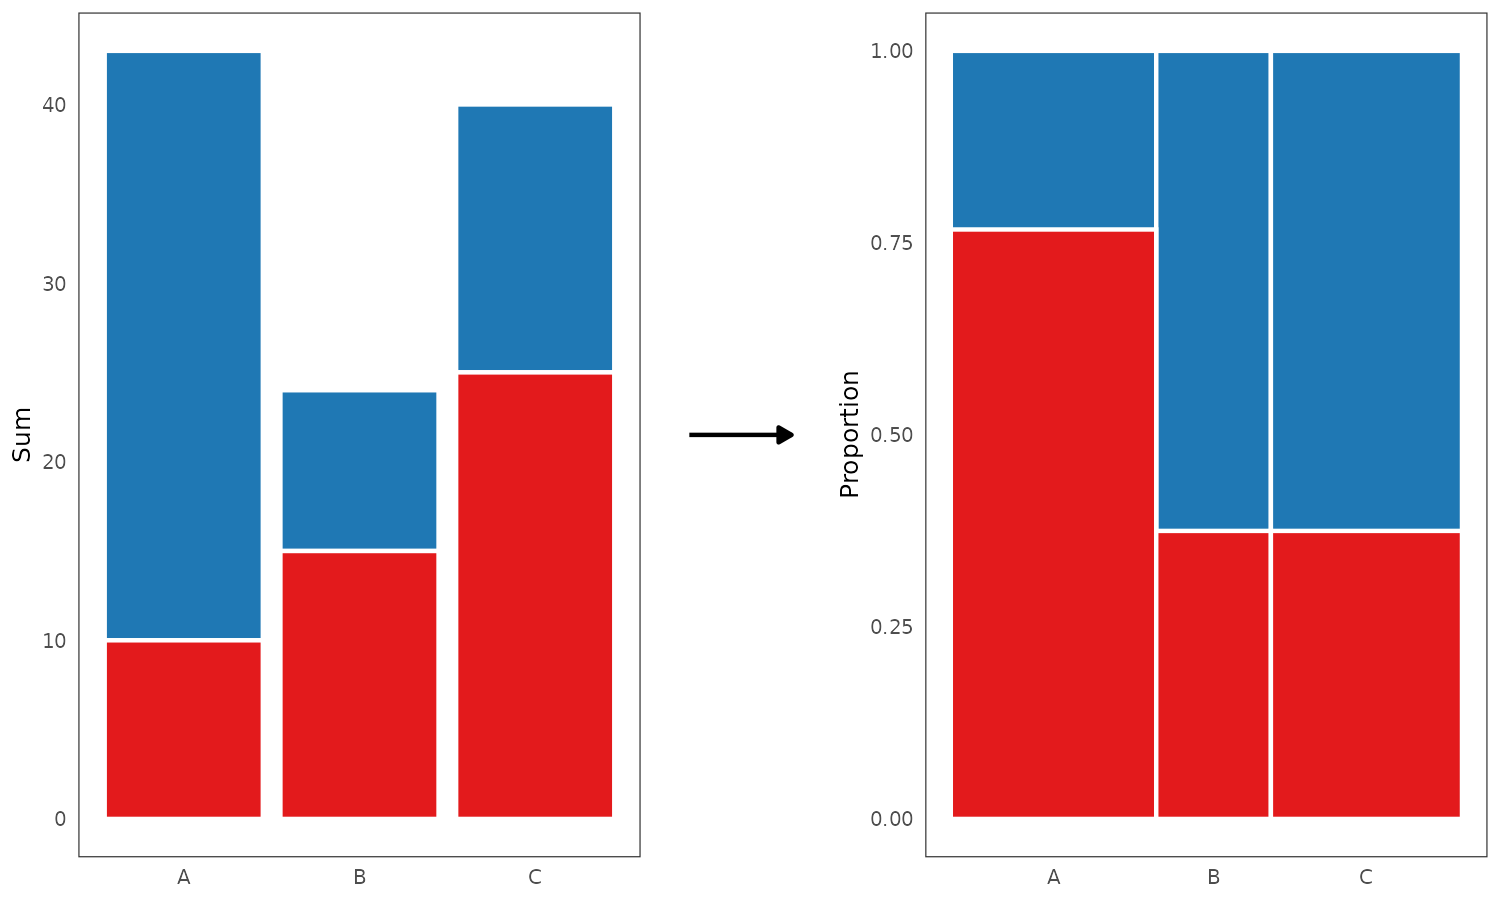
\includegraphics[width=1\linewidth,height=1\textheight]{./figures/barplot-spineplot} 

}

\caption{While barplot and spineplot represent the same underlying summaries, each makes it easier to see different aspects of our data. Barplot (left) makes it easier to compare absolute counts, whereas spineplot (right) makes it easier to compare proportions. Notice that the spineplot makes it much easier to see that the proportions of blue cases in categories B and C are exactly the same.}\label{fig:barspine}
\end{figure}

However, despite the fact that both barplots and spineplots represent the same underlying summaries (counts), turning one into the other is not always a trivial exercise. For example, in \texttt{ggplot2}, it is easy to create a barplot using simple declarative syntax, however, there is no such simple recipe for spineplots - creating the right plot in Figure \ref{fig:barspine} took over 10 lines of external data wrangling code (using standard \texttt{dplyr} syntax).

What is so complicated about spineplots? First of all, both the x- and y-axes represent the same variable: counts. However, the way the variable is used is different:

\begin{itemize}
\tightlist
\item
  Along the x-axis, we stack counts \emph{within the levels of a single factor}
\item
  Along the y-axis, we stack counts \emph{within the levels of a product of two factors} and normalize them by the counts \emph{within the levels of the parent factor}.
\end{itemize}

In other words, the spineplot forces us to confront the fact that the summaries in our plots form a hierarchy. When we compute the summaries underlying a stacked barplot or spineplot, we are not merely computing a matrix of values where the rows and the columns have no underlying meaning - instead, we are implicitly saying that objects along the x-axis (whole bars) represent a coarser level of partitioning compared with the objects (stacked segments) along the y-axis. The only difference between a barplot and spineplot is, in the barplot, we can get away with treating the two factors as if they were independent (had the same ``weight''), whereas in the spineplot this is no longer possible.

This is why in declarative data visualization systems such as \texttt{ggplot2}, certain types of plots like spineplots are difficult to express. In these systems, the data is implicitly partitioned as a ``flat'' product of the factor variables. This representation is convenient (e.g.~for defining aesthetics via a single call to \texttt{aes()}) but makes it impossible to express hierarchical structures such as the one encoded in spineplot.

Thus, ideally, our system should make it easy specify a pipeline where we compute monoidal summaries of our data within a hierarchy of partitions represented by one or more factor variables, apply some transformations to these summaries (possibly across the levels of the hierarchy), and finally map the summaries to some visual attributes.

\subsection{Scales}\label{scales}

To visualize data, we need to be able to translate values from the space of the data to the space of the graphical device (computer screen). In most data visualization systems, this is done by specialized components called scales or coordinate systems (see e.g. \citeproc{ref-murrell2005}{Murrell 2005}; \citeproc{ref-wickham2016}{Wickham 2016}; \citeproc{ref-wilkinson2012}{Wilkinson 2012}). Scales serve as a bridge between what we have (data) and what we see (visual attributes), allowing us to cross from one domain to the other.

There exists is a fair research on the theoretical properties of scales and how they relate to the mechanisms of visual perception (see e.g. \citeproc{ref-krzywinski2013}{Krzywinski 2013}; \citeproc{ref-michell1986}{Michell 1986}; \citeproc{ref-wilkinson2012}{Wilkinson 2012}; \citeproc{ref-stevens1946}{Stevens 1946}). However, when it comes to applying this knowledge and implementing scales in concrete data visualization systems, a lot less information is available. And, even when such information is available, it is it is often quite high-level of abstract (for some rare counter-examples, see e.g. \citeproc{ref-murrell2005}{Murrell 2005}; \citeproc{ref-ziemkiewicz2009}{Ziemkiewicz and Kosara 2009}). Thus, the following section is based largely on how scales have been implemented in existing data visualization codebases, such as the \texttt{ggplot2} R package (\citeproc{ref-wickham2016}{Wickham 2016}) or \texttt{d3-scale} module of D3 (\citeproc{ref-d3-scale2024}{Observable 2024}; also used by Vega \citeproc{ref-satyanarayan2015}{Satyanarayan et al. 2015}), as well as on personal insights gained while implementing the package.

\subsubsection{Overview}\label{overview}

From a high-level perspective, a scale is just a function \(s: D \to V\) which translates values of the data \(d \in D\) to values of some visual attribute \(v \in V\), such as the x- and y-position, length, area, radius, or color (\citeproc{ref-wilkinson2012}{Wilkinson 2012}). This function may or may not be invertible, such that, at times, each value of the visual attribute may be identified with a unique data value (but this is not always the case).

One of the most common and typical cases is a scale where both \(D\) and \(V\) are subsets of the real numbers:

\[s: [d_{min}, d_{max}] \to [v_{min}, v_{max}] \qquad d_{min}, d_{max}, v_{min}, v_{max} \in \mathbb{R}\]

For example, suppose our data takes values in the range from 1 to 10 and we want to plot it along the x-axis, within a 800 pixels wide plotting region. Then, our scale is simply:

\[s_x: [1, 10] \to [0, 800]\]

Now, there is an infinite number of functions that fit this signature. However, one particularly nice and simple candidate is the following function:

\begin{definition}[Simple linear mapping]
\protect\hypertarget{def:linear-mapping}{}\label{def:linear-mapping}\[s(d) = v_{max} + \frac{d - d_{min}}{d_{max} - d_{min}} \cdot (v_{max} - v_{min})\]
\end{definition}

if we substitute the concrete values into the formula, this becomes:

\[s_x(d) = 0 + \frac{d - 1}{10 - 1} \cdot (800 - 0) = [(d - 1) / 9] \cdot 800\]

The function acts on the data in the following way:

\begin{itemize}
\tightlist
\item
  \(s_x(1) = (1 - 1) / 9 \cdot 800 = 0\)
\item
  \(s_x(10) = (10 - 1) / 9 \cdot 800 = 800\)
\item
  \(s_x(d) \in (0, 800)\) for any \(d \in (1, 10)\)
\end{itemize}

That is, the function maps the data value 1 to pixel 0 (left border of the plotting region), value 10 to to pixel 800 (right border of the plotting region), and any value in between 1 and 10 inside the interval 0 to 800, proportionally to where in the data range it is located.

It is relatively simple to translate the formula in \ref{def:linear-mapping} to code:

\begin{Shaded}
\begin{Highlighting}[]
\CommentTok{// simpleScale.ts}
\ImportTok{export} \KeywordTok{function} \FunctionTok{simpleScale}\NormalTok{(}
\NormalTok{  d}\OperatorTok{:} \DataTypeTok{number}\OperatorTok{,}
\NormalTok{  dmin}\OperatorTok{:} \DataTypeTok{number}\OperatorTok{,}
\NormalTok{  dmax}\OperatorTok{:} \DataTypeTok{number}\OperatorTok{,}
\NormalTok{  vmin}\OperatorTok{:} \DataTypeTok{number}\OperatorTok{,}
\NormalTok{  vmax}\OperatorTok{:} \DataTypeTok{number}\OperatorTok{,}
\NormalTok{)}\OperatorTok{:} \DataTypeTok{number}\NormalTok{ \{}
  \ControlFlowTok{return}\NormalTok{ vmin }\OperatorTok{+}\NormalTok{ ((d }\OperatorTok{{-}}\NormalTok{ dmin) }\OperatorTok{/}\NormalTok{ (dmax }\OperatorTok{{-}}\NormalTok{ dmin)) }\OperatorTok{*}\NormalTok{ (vmax }\OperatorTok{{-}}\NormalTok{ vmin)}\OperatorTok{;}
\NormalTok{\}}
\end{Highlighting}
\end{Shaded}

And indeed, this function works the way we would expect:

\begin{Shaded}
\begin{Highlighting}[]
\ImportTok{import}\NormalTok{ \{ simpleScale \} }\ImportTok{from} \StringTok{"./simpleScale.ts"}

\BuiltInTok{console}\OperatorTok{.}\FunctionTok{log}\NormalTok{(}\FunctionTok{simpleScale}\NormalTok{(}\DecValTok{1}\OperatorTok{,} \DecValTok{1}\OperatorTok{,} \DecValTok{10}\OperatorTok{,} \DecValTok{0}\OperatorTok{,} \DecValTok{800}\NormalTok{))}
\BuiltInTok{console}\OperatorTok{.}\FunctionTok{log}\NormalTok{(}\FunctionTok{simpleScale}\NormalTok{(}\FloatTok{5.5}\OperatorTok{,} \DecValTok{1}\OperatorTok{,} \DecValTok{10}\OperatorTok{,} \DecValTok{0}\OperatorTok{,} \DecValTok{800}\NormalTok{))}
\BuiltInTok{console}\OperatorTok{.}\FunctionTok{log}\NormalTok{(}\FunctionTok{simpleScale}\NormalTok{(}\DecValTok{10}\OperatorTok{,} \DecValTok{1}\OperatorTok{,} \DecValTok{10}\OperatorTok{,} \DecValTok{0}\OperatorTok{,} \DecValTok{800}\NormalTok{))}
\end{Highlighting}
\end{Shaded}

\begin{verbatim}
## 0
## 400
## 800
\end{verbatim}

\subsubsection{Limits of modeling scales as simple functions}\label{simple-scale-limits}

Simple scale functions like the one above can work fine for basic data visualization systems. However, once we begin adding more features, this design becomes prohibitive. Consider, for example, what happens if we want to:

\begin{itemize}
\tightlist
\item
  Expand the scale limits
\item
  Scale discrete data
\item
  Apply non-linear transformations
\item
  Pan, zoom, reverse, reorder, or otherwise modify the scale interactively
\end{itemize}

Let's take the first point as a motivating example. Consider what happens to data points at the limits of the data range under the simple linear mapping:

\begin{Shaded}
\begin{Highlighting}[]
\NormalTok{x }\OtherTok{\textless{}{-}} \DecValTok{1}\SpecialCharTok{:}\DecValTok{10}
\NormalTok{y }\OtherTok{\textless{}{-}} \FunctionTok{rnorm}\NormalTok{(}\DecValTok{10}\NormalTok{, }\DecValTok{0}\NormalTok{, }\DecValTok{5}\NormalTok{)}
\NormalTok{col }\OtherTok{\textless{}{-}} \FunctionTok{ifelse}\NormalTok{(}\DecValTok{1}\SpecialCharTok{:}\DecValTok{10} \SpecialCharTok{\%in\%} \FunctionTok{c}\NormalTok{(}\DecValTok{1}\NormalTok{, }\DecValTok{10}\NormalTok{), }\StringTok{"indianred"}\NormalTok{, }\StringTok{"grey80"}\NormalTok{)}

\FunctionTok{plot}\NormalTok{(x, y, }\AttributeTok{col =}\NormalTok{ col, }\AttributeTok{cex =} \DecValTok{3}\NormalTok{, }\AttributeTok{xaxs =} \StringTok{"i"}\NormalTok{)}
\end{Highlighting}
\end{Shaded}

\begin{center}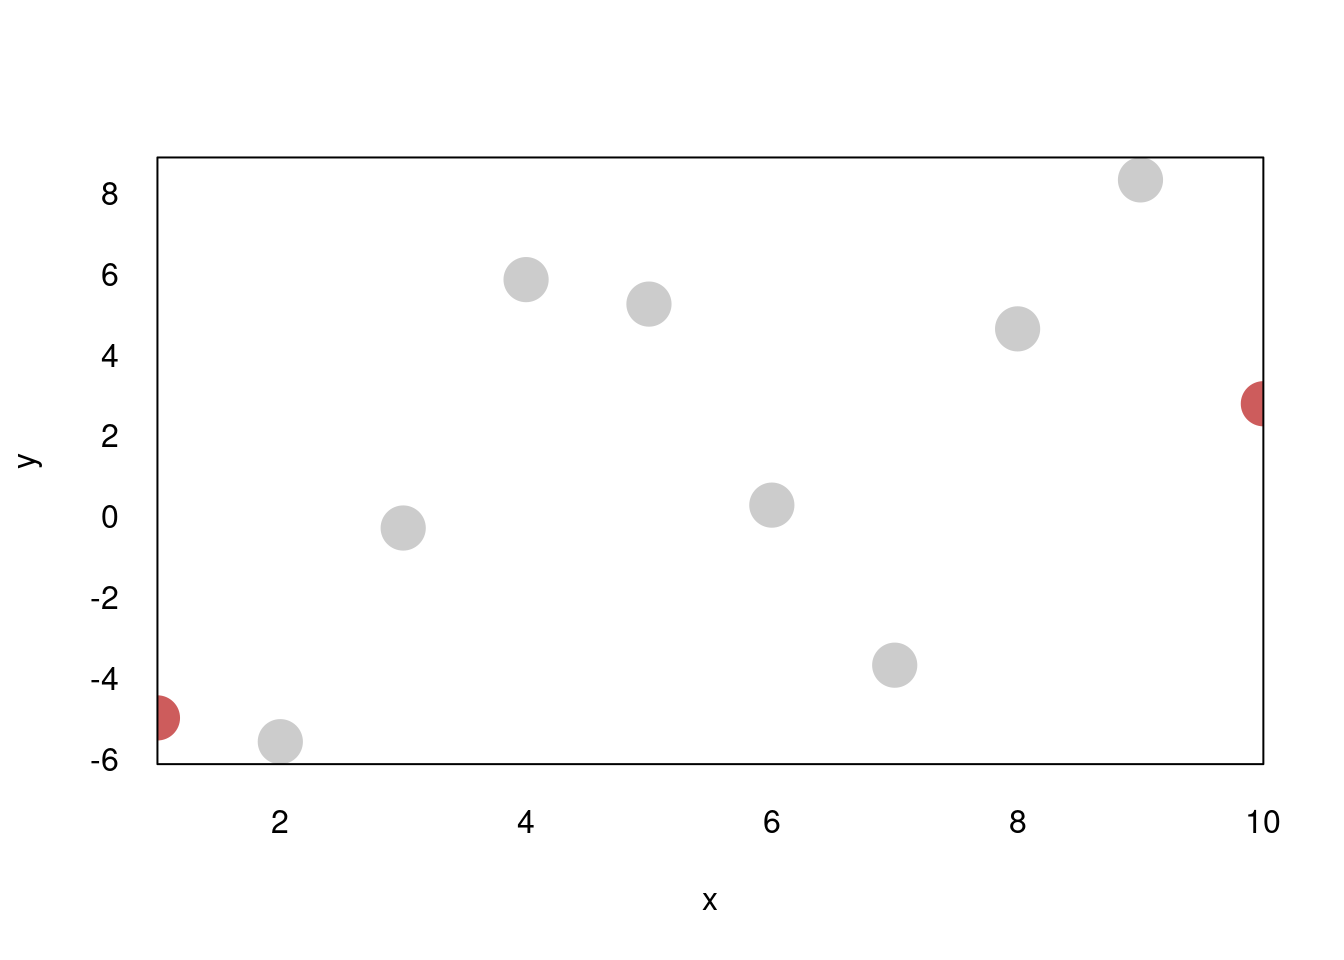
\includegraphics[width=1\linewidth,height=1\textheight]{_main_files/figure-latex/unnamed-chunk-71-1} \end{center}

The plot above shows values scaled using the simple linear mapping along the x-axis, that is, \(s: [1, 10] \to [0, 800]\) (effect of the \texttt{xaxs\ =\ "i"} argument). Notice that, since the position of the points representing the values 1 and 10 (highlighted in red) gets mapped to pixel values 0 and 800 (the left and right border of the plot), only half of each point is visible. This is quite undesirable - a fundamental principles of graphical integrity is that our graphics should not arbitrarily downplay or hide certain data points (\citeproc{ref-tufte2001}{Tufte 2001}). The points at the axis limits are represented by only 1/2 of the area (or less, if at the limits of both axes), making them less salient, and this is especially pernicious since they are likely to be outliers.

To address this problem, most data visualization systems automatically expand the range of the domain by some pre-specified percentage:

\begin{Shaded}
\begin{Highlighting}[]
\CommentTok{\# By default, the plot() function automatically expands the x{-} and y{-}axis}
\CommentTok{\# limits by approximately 4\% on each end, see \textasciigrave{}xaxs\textasciigrave{} in ?graphics::par}
\FunctionTok{plot}\NormalTok{(x, y, }\AttributeTok{col =}\NormalTok{ col, }\AttributeTok{cex =} \DecValTok{3}\NormalTok{)}
\end{Highlighting}
\end{Shaded}

\begin{center}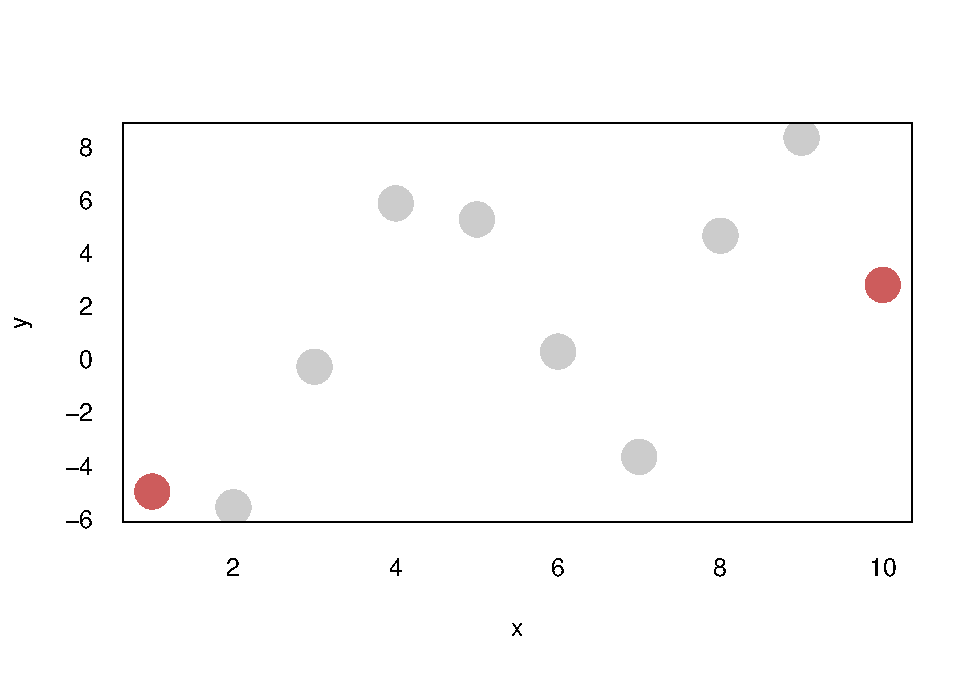
\includegraphics[width=1\linewidth,height=1\textheight]{_main_files/figure-latex/unnamed-chunk-72-1} \end{center}

We \emph{could} achieve similar effect by modifying the simple linear mapping we have defined above and adding an additional argument:

\begin{Shaded}
\begin{Highlighting}[]
\CommentTok{// simpleScale2.ts}
\ImportTok{export} \KeywordTok{function} \FunctionTok{simpleScale2}\NormalTok{(}
\NormalTok{  d}\OperatorTok{:} \DataTypeTok{number}\OperatorTok{,}
\NormalTok{  dmin}\OperatorTok{:} \DataTypeTok{number}\OperatorTok{,}
\NormalTok{  dmax}\OperatorTok{:} \DataTypeTok{number}\OperatorTok{,}
\NormalTok{  vmin}\OperatorTok{:} \DataTypeTok{number}\OperatorTok{,}
\NormalTok{  vmax}\OperatorTok{:} \DataTypeTok{number}\OperatorTok{,}
\NormalTok{  exp}\OperatorTok{:} \DataTypeTok{number}\OperatorTok{,} \CommentTok{// Extra argument}
\NormalTok{)}\OperatorTok{:} \DataTypeTok{number}\NormalTok{ \{}
  \ControlFlowTok{return}\NormalTok{ (}
\NormalTok{    vmin }\OperatorTok{+}\NormalTok{ (exp }\OperatorTok{/} \DecValTok{2} \OperatorTok{+}\NormalTok{ ((d }\OperatorTok{{-}}\NormalTok{ dmin) }\OperatorTok{/}\NormalTok{ (dmax }\OperatorTok{{-}}\NormalTok{ dmin)) }\OperatorTok{*}\NormalTok{ (}\DecValTok{1} \OperatorTok{{-}}\NormalTok{ exp)) }\OperatorTok{*}\NormalTok{ (vmax }\OperatorTok{{-}}\NormalTok{ vmin)}
\NormalTok{  )}\OperatorTok{;}
\NormalTok{\}}
\end{Highlighting}
\end{Shaded}

Now, if we set the \texttt{exp} argument to some positive value, the scaled values get mapped closer to the center of the plotting region. For example, setting \texttt{exp} to 0.2 moves each of the data limits 10\% closer to the center of the plotting region:

\begin{Shaded}
\begin{Highlighting}[]
\ImportTok{import}\NormalTok{ \{ simpleScale2 \} }\ImportTok{from} \StringTok{"./simpleScale2.ts"}

\BuiltInTok{console}\OperatorTok{.}\FunctionTok{log}\NormalTok{(}\FunctionTok{simpleScale2}\NormalTok{(}\DecValTok{1}\OperatorTok{,} \DecValTok{1}\OperatorTok{,} \DecValTok{10}\OperatorTok{,} \DecValTok{0}\OperatorTok{,} \DecValTok{800}\OperatorTok{,} \FloatTok{0.2}\NormalTok{))}\OperatorTok{;}
\BuiltInTok{console}\OperatorTok{.}\FunctionTok{log}\NormalTok{(}\FunctionTok{simpleScale2}\NormalTok{(}\FloatTok{5.5}\OperatorTok{,} \DecValTok{1}\OperatorTok{,} \DecValTok{10}\OperatorTok{,} \DecValTok{0}\OperatorTok{,} \DecValTok{800}\OperatorTok{,} \FloatTok{0.2}\NormalTok{))}\OperatorTok{;}
\BuiltInTok{console}\OperatorTok{.}\FunctionTok{log}\NormalTok{(}\FunctionTok{simpleScale2}\NormalTok{(}\DecValTok{10}\OperatorTok{,} \DecValTok{1}\OperatorTok{,} \DecValTok{10}\OperatorTok{,} \DecValTok{0}\OperatorTok{,} \DecValTok{800}\OperatorTok{,} \FloatTok{0.2}\NormalTok{))}\OperatorTok{;}
\end{Highlighting}
\end{Shaded}

\begin{verbatim}
## 80
## 400
## 720
\end{verbatim}

However, notice that this argument is applied symmetrically. At times, we may want to apply a different margin to each end of the scale. We could solve this by adding two arguments instead of one, e.g.~\texttt{expLeft} and \texttt{expRight}, however, at this point, the function signature starts to become unwieldy. If we have to call the function in multiple places, it may become difficult to remember what each individual argument represents. Further, note that by adding arguments, the logic inside the function's body becomes denser and less readable. Finally, we may want to persist or modify some of the arguments during runtime (such as when panning or zooming). For all of these reasons, it may be a good idea to take a more structured approach and break the function down into several smaller components.

\subsubsection{Solution: Two-component scales}\label{two-component-scales}

The linear mapping formula in \ref{def:linear-mapping} can guide us in decomposing the scale function into smaller, more manageable parts. Let's look at it again:

\[s(d) = v_{min} + \frac{d - d_{min}}{d_{max} - d_{min}} \cdot (v_{max} - v_{min})\]

If we look closely, we may be able to see that there are two parts to the function:

That is, the linear mapping is composed of two simpler functions:

This leads us to the following definition of a scale:

\begin{definition}[Scale as composition of two functions]
\protect\hypertarget{def:scale}{}\label{def:scale}A scale \(s\) can be created by composing:

\begin{itemize}
\tightlist
\item
  A \emph{normalize} function \(n: D \to [0, 1]\), mapping data to the interval \([0, 1]\)
\item
  An \emph{unnormalize} function \(u: [0, 1] \to V\), mapping value in \([0, 1]\) to the visual attribute codomain
\end{itemize}

Such that:

\[s(d) = u(n(d))\]
\end{definition}

Note that the terms \emph{normalize} and \emph{unnormalize} are arbitrary, however, I think they make for useful labels. They represent 1-D equivalent of vector normalization, mapping a value in the domain to and from a unit interval \([0, 1]\).

For the case of the linear mapping, we could rewrite this in code as follows:

\begin{Shaded}
\begin{Highlighting}[]
\CommentTok{// LinearMap.ts}
\ImportTok{export} \ImportTok{namespace} \DataTypeTok{LinearMap}\NormalTok{ \{}
  \ImportTok{export} \KeywordTok{function} \FunctionTok{normalize}\NormalTok{(d}\OperatorTok{:} \DataTypeTok{number}\OperatorTok{,}\NormalTok{ dmin}\OperatorTok{:} \DataTypeTok{number}\OperatorTok{,}\NormalTok{ dmax}\OperatorTok{:} \DataTypeTok{number}\NormalTok{) \{}
    \ControlFlowTok{return}\NormalTok{ (d }\OperatorTok{{-}}\NormalTok{ dmin) }\OperatorTok{/}\NormalTok{ (dmax }\OperatorTok{{-}}\NormalTok{ dmin)}\OperatorTok{;}
\NormalTok{  \}}

  \ImportTok{export} \KeywordTok{function} \FunctionTok{unnormalize}\NormalTok{(p}\OperatorTok{:} \DataTypeTok{number}\OperatorTok{,}\NormalTok{ vmin}\OperatorTok{:} \DataTypeTok{number}\OperatorTok{,}\NormalTok{ vmax}\OperatorTok{:} \DataTypeTok{number}\NormalTok{) \{}
    \ControlFlowTok{return}\NormalTok{ vmin }\OperatorTok{+}\NormalTok{ p }\OperatorTok{*}\NormalTok{ (vmax }\OperatorTok{{-}}\NormalTok{ vmin)}\OperatorTok{;}
\NormalTok{  \}}
\NormalTok{\}}
\end{Highlighting}
\end{Shaded}

\begin{Shaded}
\begin{Highlighting}[]
\ImportTok{import}\NormalTok{ \{ LinearMap \} }\ImportTok{from} \StringTok{"./LinearMap.ts"}

\BuiltInTok{console}\OperatorTok{.}\FunctionTok{log}\NormalTok{(LinearMap}\OperatorTok{.}\FunctionTok{normalize}\NormalTok{(}\FloatTok{5.5}\OperatorTok{,} \DecValTok{1}\OperatorTok{,} \DecValTok{10}\NormalTok{))}
\BuiltInTok{console}\OperatorTok{.}\FunctionTok{log}\NormalTok{(LinearMap}\OperatorTok{.}\FunctionTok{unnormalize}\NormalTok{(}\FloatTok{0.5}\OperatorTok{,} \DecValTok{0}\OperatorTok{,} \DecValTok{800}\NormalTok{))}
\BuiltInTok{console}\OperatorTok{.}\FunctionTok{log}\NormalTok{(LinearMap}\OperatorTok{.}\FunctionTok{unnormalize}\NormalTok{(LinearMap}\OperatorTok{.}\FunctionTok{normalize}\NormalTok{(}\FloatTok{5.5}\OperatorTok{,} \DecValTok{1}\OperatorTok{,} \DecValTok{10}\NormalTok{)}\OperatorTok{,} \DecValTok{0}\OperatorTok{,} \DecValTok{800}\NormalTok{))}
\end{Highlighting}
\end{Shaded}

\begin{verbatim}
## 0.5
## 400
## 400
\end{verbatim}

This two component system allows for a clean separation of concerns. Specifically, the normalize function only needs to know how to map the data values to \([0, 1]\). It does not need to be aware of where these normalized data values will be mapped to. Conversely, the unnormalize function only needs to understand how to translate values from \([0, 1]\) to the space of the visual attribute (such as x-axis position).

\paragraph{Beyond linear maps}\label{beyond-linear-maps}

Another big advantage of the two-component scale system is that the functions \(n\) and \(u\) do not need to be a simple linear maps anymore. For example, suppose that our data \(D\) takes form of a set of discrete labels, such as \(D = \{ Prague,  Vienna, Munich, Salzburg \}\). We can then replace \(n\) with a surjective function \(n: D \to [0, 1]\) such that:

\[n(d) = \begin{cases}  
0.2 & \text{if } d = Munich 
\\ 0.4 & \text{if } d = Prague 
\\ 0.6 & \text{if } d = Salzburg 
\\ 0.8 & \text{if } d = Vienna
\end{cases}\]

In other words, \(n\) will place values of \(D\) at equidistant points along \([0, 1]\), ordered alphabetically. We can implement this function in code as follows:

\begin{Shaded}
\begin{Highlighting}[]
\CommentTok{// PointMap.ts}
\ImportTok{export} \ImportTok{namespace} \DataTypeTok{PointMap}\NormalTok{ \{}
  \ImportTok{export} \KeywordTok{function} \FunctionTok{normalize}\NormalTok{(d}\OperatorTok{:} \DataTypeTok{string}\OperatorTok{,}\NormalTok{ dlabels}\OperatorTok{:} \DataTypeTok{string}\NormalTok{[]) \{}
    \ControlFlowTok{return}\NormalTok{ (dlabels}\OperatorTok{.}\FunctionTok{indexOf}\NormalTok{(d) }\OperatorTok{+} \DecValTok{1}\NormalTok{) }\OperatorTok{/}\NormalTok{ (dlabels}\OperatorTok{.}\AttributeTok{length} \OperatorTok{+} \DecValTok{1}\NormalTok{)}
\NormalTok{  \}}
\NormalTok{\}}
\end{Highlighting}
\end{Shaded}

Since the codomain of \(n\) is still \([0, 1]\), we can compose it with a simple linear mapping \(u\) just as easily as before:

\begin{Shaded}
\begin{Highlighting}[]
\ImportTok{import}\NormalTok{ \{ LinearMap \} }\ImportTok{from} \StringTok{"./LinearMap.ts"}
\ImportTok{import}\NormalTok{ \{ PointMap \} }\ImportTok{from} \StringTok{"./PointMap.ts"}

\KeywordTok{const}\NormalTok{ labels }\OperatorTok{=}\NormalTok{ [}\StringTok{"Munich"}\OperatorTok{,} \StringTok{"Prague"}\OperatorTok{,} \StringTok{"Salzburg"}\OperatorTok{,} \StringTok{"Vienna"}\NormalTok{]}\OperatorTok{;}

\BuiltInTok{console}\OperatorTok{.}\FunctionTok{log}\NormalTok{(PointMap}\OperatorTok{.}\FunctionTok{normalize}\NormalTok{(}\StringTok{"Munich"}\OperatorTok{,}\NormalTok{ labels))}\OperatorTok{;}
\BuiltInTok{console}\OperatorTok{.}\FunctionTok{log}\NormalTok{(LinearMap}\OperatorTok{.}\FunctionTok{unnormalize}\NormalTok{(PointMap}\OperatorTok{.}\FunctionTok{normalize}\NormalTok{(}\StringTok{"Munich"}\OperatorTok{,}\NormalTok{ labels)}\OperatorTok{,} \DecValTok{0}\OperatorTok{,} \DecValTok{800}\NormalTok{))}\OperatorTok{;}
\BuiltInTok{console}\OperatorTok{.}\FunctionTok{log}\NormalTok{(LinearMap}\OperatorTok{.}\FunctionTok{unnormalize}\NormalTok{(PointMap}\OperatorTok{.}\FunctionTok{normalize}\NormalTok{(}\StringTok{"Prague"}\OperatorTok{,}\NormalTok{ labels)}\OperatorTok{,} \DecValTok{0}\OperatorTok{,} \DecValTok{800}\NormalTok{))}\OperatorTok{;}
\end{Highlighting}
\end{Shaded}

\begin{verbatim}
## 0.2
## 160
## 320
\end{verbatim}

\paragraph{Inverses}\label{inverses-1}

Additionally, another property of the two-component scale system that can be useful is that, if both \(n\) and \(u\) are invertible, then so is \(s\). That is, we can easily obtain the inverse scale function by inverting the definition from \ref{def:scale}:

\begin{definition}[Scale inverse]
\protect\hypertarget{def:scale-inverse}{}\label{def:scale-inverse}If a scale \(s\) is composed of invertible functions \(n\) and \(u\), then \(s\) is invertible:

\[s^{-1}(v) = n^{-1}(u^{-1}(v))\]
\end{definition}

This is the case for the simple linear map: the normalize and unnormalize functions are actually inverses of each other:

\begin{Shaded}
\begin{Highlighting}[]
\ImportTok{import}\NormalTok{ \{ LinearMap \} }\ImportTok{from} \StringTok{"./LinearMap.ts"}

\BuiltInTok{console}\OperatorTok{.}\FunctionTok{log}\NormalTok{(LinearMap}\OperatorTok{.}\FunctionTok{unnormalize}\NormalTok{(LinearMap}\OperatorTok{.}\FunctionTok{normalize}\NormalTok{(}\DecValTok{300}\OperatorTok{,} \DecValTok{0}\OperatorTok{,} \DecValTok{500}\NormalTok{)}\OperatorTok{,} \DecValTok{0}\OperatorTok{,} \DecValTok{500}\NormalTok{))}
\end{Highlighting}
\end{Shaded}

\begin{verbatim}
## 300
\end{verbatim}

However, the inverse may not always exist. In practice, this is often the case when the domain of the data \(D\) is smaller than the codomain \([0, 1]\). Take, for example, the discrete point mapping. Since \(D\) is finite but \([0, 1]\) has infinitely many values, there will always be some values in \([0, 1]\) that no \(d \in D\) maps to. For example, if \(D = \{ Munich, Prague, Salzburg, Vienna \}\) and \(Munich\) maps to 0.2, \(Prague\) maps to \(0.4\), and \(Salzburg\) maps to \(0.8\), then there are no cities which map to 0.9, 0.444, or 0.123456789. Conversely, if we get given those numeric values, then there is no obvious way to map them back to the cities.

One thing we can do is to replace the inverse/unnormalize function with a weaker form of inverse, called retraction (\citeproc{ref-lawvere2009}{Lawvere and Schanuel 2009}). Specifically, if we have a normalize function \(n: D \to [0, 1]\), then an unnormalize retraction \(u^*\) will have the property that:

\[u^*(n(d)) = d \qquad \forall d \in D\]

However, the converse doesn't necessarily hold:

\[\neg \big[ n(u^*(v)) = v \qquad \forall v \in V \big]\]

For example, for the discrete point mapping, a retraction may map a value in \([0, 1]\) to the closest data value \(d \in D\):

\begin{Shaded}
\begin{Highlighting}[]
\CommentTok{// PointMap.ts}
\ImportTok{export} \ImportTok{namespace} \DataTypeTok{PointMap}\NormalTok{ \{}
  \ImportTok{export} \KeywordTok{function} \FunctionTok{normalize}\NormalTok{(d}\OperatorTok{:} \DataTypeTok{string}\OperatorTok{,}\NormalTok{ dlabels}\OperatorTok{:} \DataTypeTok{string}\NormalTok{[]) \{}
    \ControlFlowTok{return}\NormalTok{ (dlabels}\OperatorTok{.}\FunctionTok{indexOf}\NormalTok{(d) }\OperatorTok{+} \DecValTok{1}\NormalTok{) }\OperatorTok{/}\NormalTok{ (dlabels}\OperatorTok{.}\AttributeTok{length} \OperatorTok{+} \DecValTok{1}\NormalTok{)}
\NormalTok{  \}}
  
  \CommentTok{// Retraction {-} find the closest label}
  \ImportTok{export} \KeywordTok{function} \FunctionTok{unnormalize}\NormalTok{(p}\OperatorTok{:} \DataTypeTok{number}\OperatorTok{,}\NormalTok{ dlabels}\OperatorTok{:} \DataTypeTok{string}\NormalTok{[]) \{}
    \KeywordTok{const}\NormalTok{ k }\OperatorTok{=} \BuiltInTok{Math}\OperatorTok{.}\FunctionTok{round}\NormalTok{(p }\OperatorTok{*}\NormalTok{ (dlabels}\OperatorTok{.}\AttributeTok{length} \OperatorTok{+} \DecValTok{1}\NormalTok{) }\OperatorTok{{-}} \DecValTok{1}\NormalTok{)}
    \ControlFlowTok{return}\NormalTok{ dlabels[k]}
\NormalTok{  \}}
\NormalTok{\}}

\KeywordTok{const}\NormalTok{ labels }\OperatorTok{=}\NormalTok{ [}\StringTok{"Munich"}\OperatorTok{,} \StringTok{"Prague"}\OperatorTok{,} \StringTok{"Salzburg"}\OperatorTok{,} \StringTok{"Vienna"}\NormalTok{]}\OperatorTok{;}

\KeywordTok{const}\NormalTok{ [prague}\OperatorTok{,}\NormalTok{ munich] }\OperatorTok{=}\NormalTok{ [}\StringTok{"Prague"}\OperatorTok{,} \StringTok{"Munich"}\NormalTok{]}\OperatorTok{.}\FunctionTok{map}\NormalTok{(x }\KeywordTok{=\textgreater{}}\NormalTok{ PointMap}\OperatorTok{.}\FunctionTok{normalize}\NormalTok{(x}\OperatorTok{,}\NormalTok{ labels))}
\KeywordTok{const}\NormalTok{ midpoint }\OperatorTok{=}\NormalTok{ (prague }\OperatorTok{+}\NormalTok{ munich) }\OperatorTok{/} \DecValTok{2}

\CommentTok{// Helper function for stripping away floating point error }
\KeywordTok{const}\NormalTok{ strip }\OperatorTok{=}\NormalTok{ (x}\OperatorTok{:} \DataTypeTok{number}\NormalTok{) }\KeywordTok{=\textgreater{}} \PreprocessorTok{parseFloat}\NormalTok{(x}\OperatorTok{.}\FunctionTok{toPrecision}\NormalTok{(}\DecValTok{12}\NormalTok{))}

\BuiltInTok{console}\OperatorTok{.}\FunctionTok{log}\NormalTok{(}\VerbatimStringTok{\textasciigrave{}Midpoint between Munich and Prague: \textasciigrave{}}\OperatorTok{,} \FunctionTok{strip}\NormalTok{(midpoint))}
\BuiltInTok{console}\OperatorTok{.}\FunctionTok{log}\NormalTok{(}\VerbatimStringTok{\textasciigrave{}unnormalize(0.2999): \textasciigrave{}}\OperatorTok{,}\NormalTok{ PointMap}\OperatorTok{.}\FunctionTok{unnormalize}\NormalTok{(}\FloatTok{0.2999}\OperatorTok{,}\NormalTok{ labels))}
\BuiltInTok{console}\OperatorTok{.}\FunctionTok{log}\NormalTok{(}\VerbatimStringTok{\textasciigrave{}unnormalize(3): \textasciigrave{}}\OperatorTok{,}\NormalTok{ PointMap}\OperatorTok{.}\FunctionTok{unnormalize}\NormalTok{(}\FloatTok{0.3}\OperatorTok{,}\NormalTok{ labels))}
\end{Highlighting}
\end{Shaded}

\begin{verbatim}
## Midpoint between Munich and Prague:  0.3
## unnormalize(0.2999):  Munich
## unnormalize(3):  Prague
\end{verbatim}

While inverses are always unique (\citeproc{ref-lawvere2009}{Lawvere and Schanuel 2009}; \citeproc{ref-fong2019}{Fong and Spivak 2019}), we may be able to come up with many different retractions for any given function. For example, with the discrete point map above, we could use the floor function instead of rounding and assign label to a value in \([0, 1]\) if it is less than the value of the normalized label (but more than the preceding labels).

The non-uniqueness of retractions presents a bit of a dilemma. How do we decide which retraction to use? And, if a certain retractive implementation of \texttt{unnormalize} returns a value, how do we decide if it is the ``correct one''?

However, in practice, this is not much of a problem. While developing the package, I found that I've only ever had to use the \texttt{unnormalize} function with continuous data (\texttt{LinearMap}), and so the inverse was always well-defined. This is probably also why packages like \texttt{ggplot2} and \texttt{D3} can get by without this functionality. However, I still find it helpful to include the \texttt{unnormalize} function as a first class citizen (instead of it being relegated to some special case), both in terms of the mental model and also for debugging.

\paragraph{Some other remarks about the two-component scale system}\label{some-other-remarks-about-the-two-component-scale-system}

It is worth noting that there is nothing inherently special about the interval \([0, 1]\) as the intermediate domain: any finite subset of \(\mathbb{R}\) would do. However, the interval \([0, 1]\) is convenient, both in terms of interpretation as well as for implementation, as we will see later.

Finally, so far I have discussed scales as \emph{functions}: the scale function, the normalize function, and unnormalize function. Framing scales as composition of functions leads to a nice correspondence between the mathematical definition and the code. However, in practice, it may be more convenient to implement the domain and codomain as \emph{objects} or \emph{classes}, as we will also see in the following section. The important point is that, no matter how the two components are represented, each is responsible for translating values from/to its domain and the interval \([0, 1]\).

\subsubsection{Past implementations of scales}\label{past-implementations-of-scales}

Two-component scale systems such as the one sketched out above are fairly standard across data visualization libraries. For example, in \texttt{D3} (\citeproc{ref-bostock2011}{Michael Bostock, Ogievetsky, and Heer 2011}), scales are implemented in a functional style, such that the data domain and the visual attribute codomain are passed as tuples or arrays of values to a higher-order \texttt{scale*} function (such as \texttt{scaleLinear}, \texttt{scalePoint}, or \texttt{scaleBand}), which then returns a new function that can be used for scaling. The domain and codomain can also be changed at a later point, by using the \texttt{scale*.domain} and \texttt{scale*.range} methods respectively (JavaScript functions are objects and can have other functions/methods attached to them).

For illustration, here is an example from the official documentation (\citeproc{ref-d3-scale2024}{Observable 2024}):

\begin{Shaded}
\begin{Highlighting}[]
\KeywordTok{const}\NormalTok{ x }\OperatorTok{=}\NormalTok{ d3}\OperatorTok{.}\FunctionTok{scaleLinear}\NormalTok{([}\DecValTok{10}\OperatorTok{,} \DecValTok{130}\NormalTok{]}\OperatorTok{,}\NormalTok{ [}\DecValTok{0}\OperatorTok{,} \DecValTok{960}\NormalTok{])}\OperatorTok{;}
\FunctionTok{x}\NormalTok{(}\DecValTok{20}\NormalTok{)}\OperatorTok{;} \CommentTok{// 80}
\KeywordTok{const}\NormalTok{ color }\OperatorTok{=}\NormalTok{ d3}\OperatorTok{.}\FunctionTok{scaleLinear}\NormalTok{([}\DecValTok{10}\OperatorTok{,} \DecValTok{100}\NormalTok{]}\OperatorTok{,}\NormalTok{ [}\StringTok{"brown"}\OperatorTok{,} \StringTok{"steelblue"}\NormalTok{])}\OperatorTok{;}
\FunctionTok{color}\NormalTok{(}\DecValTok{20}\NormalTok{)}\OperatorTok{;} \CommentTok{// "rgb(154, 52, 57)"}
\CommentTok{// The domain and codomain can be changed after initialization}
\KeywordTok{const}\NormalTok{ y }\OperatorTok{=}\NormalTok{ d3}\OperatorTok{.}\FunctionTok{scaleLinear}\NormalTok{()}\OperatorTok{.}\FunctionTok{domain}\NormalTok{([}\DecValTok{10}\OperatorTok{,} \DecValTok{130}\NormalTok{])}\OperatorTok{;} 
\end{Highlighting}
\end{Shaded}

Internally, the \texttt{scale*} functions rely on other specialized functions to translate from its domain to the codomain (such as the \texttt{normalize()} and \texttt{scale()} functions for continuous and discrete/ordinal domains, respectively, and various \texttt{interpolate()} functions for codomains).

Similarly, in \texttt{ggplot2} (\citeproc{ref-wickham2016}{Wickham 2016}), scales are built upon the \texttt{Scale} class, with each subtype implementing \texttt{limits} and \texttt{palette} properties. The \texttt{limits} property is a vector which corresponds to the data domain and the \texttt{palette} property is a function which corresponds roughly to the visual codomain (the x- and y-position behave slightly differently, due to being transformed via coordinate systems). Internally, the package uses the \texttt{rescale} function from the \texttt{scales} package (\citeproc{ref-wickham2023}{Wickham, Pedersen, and Seidel 2023}) to map data values to \([0, 1]\) and then the \texttt{palette} function is responsible for mapping these normalized values to the visual attribute. For illustration, here's the full definition of the \texttt{map} method on the \texttt{ScaleContinuous} class (I've added comments for clarity):

\begin{Shaded}
\begin{Highlighting}[]
\NormalTok{map }\OtherTok{=} \ControlFlowTok{function}\NormalTok{(self, x, }\AttributeTok{limits =}\NormalTok{ self}\SpecialCharTok{$}\FunctionTok{get\_limits}\NormalTok{()) \{}
  \CommentTok{\# Limits are just a tuple, rescale maps x to [0, 1]}
\NormalTok{  x }\OtherTok{\textless{}{-}}\NormalTok{ self}\SpecialCharTok{$}\FunctionTok{rescale}\NormalTok{(self}\SpecialCharTok{$}\FunctionTok{oob}\NormalTok{(x, }\AttributeTok{range =}\NormalTok{ limits), limits) }

\NormalTok{  uniq }\OtherTok{\textless{}{-}} \FunctionTok{unique0}\NormalTok{(x)}
  \CommentTok{\# Palette is a function which returns a vector of attribute values}
\NormalTok{  pal }\OtherTok{\textless{}{-}}\NormalTok{ self}\SpecialCharTok{$}\FunctionTok{palette}\NormalTok{(uniq) }
\NormalTok{  scaled }\OtherTok{\textless{}{-}}\NormalTok{ pal[}\FunctionTok{match}\NormalTok{(x, uniq)]}

  \FunctionTok{ifelse}\NormalTok{(}\SpecialCharTok{!}\FunctionTok{is.na}\NormalTok{(scaled), scaled, self}\SpecialCharTok{$}\NormalTok{na.value)}
\NormalTok{\}}
\end{Highlighting}
\end{Shaded}

\subsubsection{Proposed model of scales}\label{proposed-model-of-scales}

One feature that the models of scales that \texttt{D3} and \texttt{ggplot2} rely on is that they both treat the data domain and the visual attribute codomain as different types. In \texttt{D3}, fundamentally different functions are used to translate from \(D \to [0, 1]\) and from \([0, 1] \to V\), and in \texttt{ggplot2}, \texttt{limits} is a simple vector/tuple whereas \texttt{palette} is a function. While these approaches may have some benefits, such as perhaps offering greater flexibility, they also add additional complexity. Specifically, we have to use two different mental models: one when considering the domain and another when considering the codomain. Further, these models of scales only work in one direction: mapping values \(D \to V\). For going the the other way, i.e.~mapping \(V \to D\), other specialized functions have to be used.

I propose a model of scales which implements both the domain and the codomain as components of the same type: \texttt{Expanse}. Fundamentally, this makes it so that the only difference between the data domain and the visual attribute codomain is which property of the scale they are assigned to.

Here is a (slightly) simplified version of the \texttt{Scale} interface:

\begin{Shaded}
\begin{Highlighting}[]
\KeywordTok{interface}\NormalTok{ Scale}\OperatorTok{\textless{}}\NormalTok{D }\KeywordTok{extends}\NormalTok{ Expanse}\OperatorTok{,}\NormalTok{ V }\KeywordTok{extends}\NormalTok{ Expanse}\OperatorTok{\textgreater{}}\NormalTok{ \{}
\NormalTok{  domain}\OperatorTok{:}\NormalTok{ D}
\NormalTok{  codomain}\OperatorTok{:}\NormalTok{ V}
\NormalTok{\}}
\end{Highlighting}
\end{Shaded}

\texttt{D} and \texttt{V} represent the data domain and the visual attribute codomain, respectively.

The two fundamental functions connected to \texttt{Scale} are:

\begin{Shaded}
\begin{Highlighting}[]
\KeywordTok{function} \FunctionTok{pushforward}\OperatorTok{\textless{}}\NormalTok{D}\OperatorTok{,}\NormalTok{ V}\OperatorTok{\textgreater{}}\NormalTok{(scale}\OperatorTok{:}\NormalTok{ Scale}\OperatorTok{\textless{}}\NormalTok{D}\OperatorTok{,}\NormalTok{ V}\OperatorTok{\textgreater{},}\NormalTok{ value}\OperatorTok{:}\NormalTok{ ValueOf}\OperatorTok{\textless{}}\NormalTok{D}\OperatorTok{\textgreater{}}\NormalTok{)}\OperatorTok{:}\NormalTok{ ValueOf}\OperatorTok{\textless{}}\NormalTok{V}\OperatorTok{\textgreater{}}
\KeywordTok{function} \FunctionTok{pullback}\OperatorTok{\textless{}}\NormalTok{D}\OperatorTok{,}\NormalTok{ V}\OperatorTok{\textgreater{}}\NormalTok{(scale}\OperatorTok{:}\NormalTok{ Scale}\OperatorTok{\textless{}}\NormalTok{D}\OperatorTok{,}\NormalTok{ V}\OperatorTok{\textgreater{},}\NormalTok{ value}\OperatorTok{:}\NormalTok{ ValueOf}\OperatorTok{\textless{}}\NormalTok{V}\OperatorTok{\textgreater{}}\NormalTok{)}\OperatorTok{:}\NormalTok{ ValueOf}\OperatorTok{\textless{}}\NormalTok{D}\OperatorTok{\textgreater{}}
\end{Highlighting}
\end{Shaded}

The \texttt{pushforward} function \emph{pushes values forward} through the scale, first through its domain and then its codomain, and the \texttt{pullback} function \emph{pulls values back}, first through its codomain and then through its domain. The \texttt{ValueOf} type helper just identifies the type associated with the expanse's data (e.g.~\texttt{number} for a continuous \texttt{Expanse}, \texttt{string} for a discrete \texttt{Expanse}, etc\ldots). I've omitted the generic type parameter constraint (\texttt{\textless{}D\ extends\ Expanse,\ V\ extends\ Expanse\textgreater{}}) for brevity.

Here is a simplified implementation of the two functions:

\begin{Shaded}
\begin{Highlighting}[]
\ImportTok{namespace} \DataTypeTok{Scale}\NormalTok{ \{}
  \KeywordTok{function} \FunctionTok{pushforward}\OperatorTok{\textless{}}\NormalTok{D}\OperatorTok{,}\NormalTok{ V}\OperatorTok{\textgreater{}}\NormalTok{(scale}\OperatorTok{:}\NormalTok{ Scale}\OperatorTok{\textless{}}\NormalTok{D}\OperatorTok{,}\NormalTok{ V}\OperatorTok{\textgreater{},}\NormalTok{ value}\OperatorTok{:}\NormalTok{ ValueOf}\OperatorTok{\textless{}}\NormalTok{D}\OperatorTok{\textgreater{}}\NormalTok{)}\OperatorTok{:}\NormalTok{ ValueOf}\OperatorTok{\textless{}}\NormalTok{V}\OperatorTok{\textgreater{}}\NormalTok{ \{}
    \KeywordTok{const}\NormalTok{ \{ domain}\OperatorTok{,}\NormalTok{ codomain \} }\OperatorTok{=}\NormalTok{ scale}\OperatorTok{;}
    \ControlFlowTok{return}\NormalTok{ Expanse}\OperatorTok{.}\FunctionTok{unnormalize}\NormalTok{(codomain}\OperatorTok{,}\NormalTok{ Expanse}\OperatorTok{.}\FunctionTok{normalize}\NormalTok{(domain}\OperatorTok{,}\NormalTok{ value))}\OperatorTok{;}
\NormalTok{  \}}

  \KeywordTok{function} \FunctionTok{pullback}\OperatorTok{\textless{}}\NormalTok{D}\OperatorTok{,}\NormalTok{ V}\OperatorTok{\textgreater{}}\NormalTok{(scale}\OperatorTok{:}\NormalTok{ Scale}\OperatorTok{\textless{}}\NormalTok{D}\OperatorTok{,}\NormalTok{ V}\OperatorTok{\textgreater{},}\NormalTok{ value}\OperatorTok{:}\NormalTok{ ValueOf}\OperatorTok{\textless{}}\NormalTok{V}\OperatorTok{\textgreater{}}\NormalTok{)}\OperatorTok{:}\NormalTok{ ValueOf}\OperatorTok{\textless{}}\NormalTok{D}\OperatorTok{\textgreater{}}\NormalTok{ \{}
    \KeywordTok{const}\NormalTok{ \{ domain}\OperatorTok{,}\NormalTok{ codomain \} }\OperatorTok{=}\NormalTok{ scale}\OperatorTok{;}
    \ControlFlowTok{return}\NormalTok{ Expanse}\OperatorTok{.}\FunctionTok{unnormalize}\NormalTok{(domain}\OperatorTok{,}\NormalTok{ Expanse}\OperatorTok{.}\FunctionTok{normalize}\NormalTok{(codomain}\OperatorTok{,}\NormalTok{ value))}
\NormalTok{  \}}
\NormalTok{\}}
\end{Highlighting}
\end{Shaded}

We can see that most of the work is done by the two \texttt{Expanse} components: we use \texttt{domain} to translates \(D \to [0, 1]\) and codomain to translate \([0, 1] \to V\). \texttt{Scale} only serves as plumbing, connecting the two together.

I argue that this model provides several benefits. First of all, it makes the code easier to reason about. Since both the \texttt{domain} and \texttt{codomain} are of the same type, we only need to keep a single mental model in mind. Second, if \texttt{domain} and \texttt{codomain} provide inverse functions (\texttt{unnormalize}), we get the inverse scale function \(V \to D\) for free (this is just the \texttt{pullback} function).

However, before we discuss \texttt{Expanse}, there are also some important functionalities that we may want to implement on \texttt{Scale} directly. There are two main reasons for this. First, we may want these functionalities to apply generally, across the various \texttt{Expanse} subtypes. Second, by implementing them on \texttt{Scale}, we can keep the \texttt{Expanse} interface cleaner. These general functionalities will be the subject of the next few sections.

\paragraph{Zero and one}\label{zero-and-one}

Recall how in Section \ref{simple-scale-limits}, we discussed the problem of expanding axis limits to display margins. Clearly, this is something that we also want to be able to do with our two-component scales. However, since we are designing an interactive data visualization system, we also want to be able to do more with axis limits: we want to be able to manipulate them dynamically during runtime, to implement features such as zooming and panning.

In Section \ref{simple-scale-limits}, we solved the problem of expanding axis limits by adding an additional argument to the \texttt{simpleScale} function. However, as was discussed previously, this approach does not scale well for more featureful implementations of scales. So how should we go about implementing dynamic axis limits in the context of the two-component scale system?

Suppose we want to add margins to a scale where both the domain or codomain are continuous, such as the x-axis in a typical scatterplot. To implement margins, we could either expand the range of the data (the domain) or shrink the range of the visual attribute (the codomain). However, expanding the domain seems like a bad idea - this only works if the domain is continuous, and, clearly, we may want to add margins to discrete scales too, such the the x-axis of a barplot. Shrinking the range of the codomain could work (most visual attributes are continuous), however, we would need to implement some custom logic for when the plot gets resized. Also, by treating codomain differently than the codomain, we would be breaking away from our intention of representing both with the same generic \texttt{Expanse} type.

So what can we do? As was foreshadowed at end of the previous section, we can put the functionality for expanding axis limits directly onto \texttt{Scale}. Specifically, notice that any values passing through a scale are first converted to the interval \([0, 1]\) and then back to the space of either the domain or codomain:

\[D \to [0, 1] \to V\]

If we re-normalize these normalized values in \([0, 1]\), we effectively expand or shrink axis limits without having to touch either the domain or codomain. To give a metaphor, if we imagine \texttt{Scale} as a pipe connecting the \texttt{domain} and \texttt{codomain}, we can manipulate axis limits by stretching or squeezing this pipe, allowing more or less water to flow through.

To actually implement this, we can add two additional parameters to \texttt{Scale}, \texttt{zero} and \texttt{one}:

\begin{Shaded}
\begin{Highlighting}[]
\KeywordTok{interface}\NormalTok{ Scale}\OperatorTok{\textless{}}\NormalTok{D }\KeywordTok{extends}\NormalTok{ Expanse}\OperatorTok{,}\NormalTok{ V }\KeywordTok{extends}\NormalTok{ Expanse}\OperatorTok{\textgreater{}}\NormalTok{ \{}
\NormalTok{  domain}\OperatorTok{:}\NormalTok{ D}
\NormalTok{  codomain}\OperatorTok{:}\NormalTok{ V}
\NormalTok{  props}\OperatorTok{:}\NormalTok{ \{ }\CommentTok{// A dictionary of properties}
\NormalTok{    zero}\OperatorTok{:} \DataTypeTok{number}
\NormalTok{    one}\OperatorTok{:} \DataTypeTok{number}
\NormalTok{  \}}
\NormalTok{\}}
\end{Highlighting}
\end{Shaded}

Now, we can use these two parameters to implement a new version of the \texttt{pushforward} function:

\begin{Shaded}
\begin{Highlighting}[]
\KeywordTok{function} \FunctionTok{pushforward}\OperatorTok{\textless{}}\NormalTok{D}\OperatorTok{,}\NormalTok{ V}\OperatorTok{\textgreater{}}\NormalTok{(scale}\OperatorTok{:}\NormalTok{ Scale}\OperatorTok{\textless{}}\NormalTok{D}\OperatorTok{,}\NormalTok{ V}\OperatorTok{\textgreater{},}\NormalTok{ value}\OperatorTok{:}\NormalTok{ D)}\OperatorTok{:}\NormalTok{ V \{}
  \KeywordTok{const}\NormalTok{ \{ domain}\OperatorTok{,}\NormalTok{ codomain}\OperatorTok{,}\NormalTok{ props \} }\OperatorTok{=}\NormalTok{ scale}\OperatorTok{;}
  \KeywordTok{const}\NormalTok{ \{ zero}\OperatorTok{,}\NormalTok{ one \} }\OperatorTok{=}\NormalTok{ props}
  \KeywordTok{let}\NormalTok{ normalized }\OperatorTok{=}\NormalTok{ Expanse}\OperatorTok{.}\FunctionTok{normalize}\NormalTok{(domain}\OperatorTok{,}\NormalTok{ value)}
\NormalTok{  normalized }\OperatorTok{=}\NormalTok{ zero }\OperatorTok{+}\NormalTok{ normalized }\OperatorTok{*}\NormalTok{ (one }\OperatorTok{{-}}\NormalTok{ zero) }\CommentTok{// Re{-}normalize}
  \ControlFlowTok{return}\NormalTok{ Expanse}\OperatorTok{.}\FunctionTok{unnormalize}\NormalTok{(codomain}\OperatorTok{,}\NormalTok{ normalized)}
\NormalTok{\}}
\end{Highlighting}
\end{Shaded}

The new function's body is a bit more dense, however, the only real change is in the line with the comment. When we re-normalize, we scale the normalized value by the \texttt{(zero\ -\ one)} range and increment it by \texttt{zero}. In other words, \texttt{zero} tells us the proportion of the codomain range that the minimum data value gets mapped to, and \texttt{one} tells us the proportion of the codomain range that the maximum data value gets mapped to.

For example, suppose we set \texttt{zero} to 0.1 and \texttt{one} to 0.9. Then we have effectively implemented 10\% margins on either side of the scale. If our scale has a \([1, 10]\) domain and \([0, 800]\) codomain, this will result in the following mapping:

\begin{itemize}
\tightlist
\item
  The ``minimum'' data value (1) gets mapped to 10\% of the codomain range (80)

  \begin{itemize}
  \tightlist
  \item
    Because \texttt{zero\ +\ 0\ *\ (one\ -\ zero)\ =\ zero\ =\ 0.1}
  \end{itemize}
\item
  The ``maximum'' data value (10) gets mapped to 90\% of the codomain range (720)

  \begin{itemize}
  \tightlist
  \item
    Because \texttt{zero\ +\ 1\ *\ (one\ -\ zero)\ =\ one\ =\ 0.9}
  \end{itemize}
\end{itemize}

Note the quotation marks around the words ``minimum'' and ``maximum'' - there is no requirement for the data to be continuous. For example, if the domain is a discrete \texttt{Expanse} which maps the string value \texttt{"A"} to zero, then the \texttt{pushforward} function will map \texttt{"A"} to 10\% of the codomain range, just as it did in the case of the continuous domain. Likewise, the codomain could also be discrete - we could use this to implement scales for binned versions of visual attributes such as color or size.

Thus, we can use \texttt{zero} and \texttt{one} to implement margins. However, there is much more we can do with these parameters. First, despite the names, \texttt{zero} and \texttt{one} can both take values \emph{less} than zero and \emph{more} than one. For example, suppose we increment both \texttt{zero} and \texttt{one} by the same amount, e.g.~we set \texttt{zero} to 0.1 and \texttt{one} to 1.1. Then, the minimum data value will get mapped to the 10\% of the codomain range, and the maximum data value will get mapped to 110\% of the codomain range (which may lie outside the space representable by the graphic device). If the codomain represents the x-axis position, then we have shifted all of the geometric objects 10\% to the right. We have effectively implemented \emph{panning}:

\begin{Shaded}
\begin{Highlighting}[]
\KeywordTok{function} \FunctionTok{move}\NormalTok{(scale}\OperatorTok{:}\NormalTok{ Scale}\OperatorTok{,}\NormalTok{ amount}\OperatorTok{:} \DataTypeTok{number}\NormalTok{) \{}
\NormalTok{  scale}\OperatorTok{.}\AttributeTok{props}\OperatorTok{.}\AttributeTok{zero} \OperatorTok{+=}\NormalTok{ amount}\OperatorTok{;}
\NormalTok{  scale}\OperatorTok{.}\AttributeTok{props}\OperatorTok{.}\AttributeTok{one} \OperatorTok{+=}\NormalTok{ amount}\OperatorTok{;}
\NormalTok{\}}
\end{Highlighting}
\end{Shaded}

That's it. We have implemented a functionality for panning which will work no matter if \texttt{domain} translates numbers, strings, or some other more complex data types.

We can also stretch or shrink \texttt{zero} and \texttt{one} in opposite directions. For example, by setting \texttt{zero} to -0.5 and \texttt{one} to 1.5, then the minimum and maximum data values will get mapped 50\% below and 50\% above the limits of the codomain range, respectively, and the 25 and 75 data percentiles will get mapped to the minimum and maximum of the codomain range. If we apply this to the x- or y-axes, we've just implemented \emph{zooming}.

To be perfectly honest, there's a bit more ceremony involved with zooming. Specifically, if we don't start from \texttt{zero\ =\ 0} and \texttt{one\ =\ 1} (e.g.~if our plot already has margins or if we're zooming in multiple levels deep), then we need to re-normalize within these values. This took me a bit of time to nail down, however, it's just (highschool) algebra:

\begin{Shaded}
\begin{Highlighting}[]
\KeywordTok{function} \FunctionTok{rangeInverse}\NormalTok{(min}\OperatorTok{:} \DataTypeTok{number}\OperatorTok{,}\NormalTok{ max}\OperatorTok{:} \DataTypeTok{number}\NormalTok{) \{}
  \ControlFlowTok{return} \DecValTok{1} \OperatorTok{/}\NormalTok{ (max }\OperatorTok{{-}}\NormalTok{ min)}\OperatorTok{;}
\NormalTok{\}}

\KeywordTok{function} \FunctionTok{invertRange}\NormalTok{(min}\OperatorTok{:} \DataTypeTok{number}\OperatorTok{,}\NormalTok{ max}\OperatorTok{:} \DataTypeTok{number}\NormalTok{) \{}
  \KeywordTok{const}\NormalTok{ ri }\OperatorTok{=} \FunctionTok{rangeInverse}\NormalTok{(min}\OperatorTok{,}\NormalTok{ max)}\OperatorTok{;}
  \ControlFlowTok{return}\NormalTok{ [}\OperatorTok{{-}}\NormalTok{min }\OperatorTok{*}\NormalTok{ ri}\OperatorTok{,}\NormalTok{ ri }\OperatorTok{{-}}\NormalTok{ min }\OperatorTok{*}\NormalTok{ ri]}\OperatorTok{;}
\NormalTok{\}}

\ImportTok{namespace} \DataTypeTok{Scale}\NormalTok{ \{}
  \ImportTok{export} \KeywordTok{function} \FunctionTok{expand}\NormalTok{(}
\NormalTok{    scale}\OperatorTok{:}\NormalTok{ \{ props}\OperatorTok{:}\NormalTok{ \{ zero}\OperatorTok{:} \DataTypeTok{number}\OperatorTok{;}\NormalTok{ one}\OperatorTok{:} \DataTypeTok{number}\NormalTok{ \} \}}\OperatorTok{,}
\NormalTok{    zero}\OperatorTok{:} \DataTypeTok{number}\OperatorTok{,}
\NormalTok{    one}\OperatorTok{:} \DataTypeTok{number}
\NormalTok{  ) \{}
    \KeywordTok{const}\NormalTok{ \{ zero}\OperatorTok{:}\NormalTok{ currentZero}\OperatorTok{,}\NormalTok{ one}\OperatorTok{:}\NormalTok{ currentOne \} }\OperatorTok{=}\NormalTok{ scale}\OperatorTok{.}\AttributeTok{props}\OperatorTok{;}
    \KeywordTok{const}\NormalTok{ currentRange }\OperatorTok{=}\NormalTok{ currentOne }\OperatorTok{{-}}\NormalTok{ currentZero}\OperatorTok{;}
    
    \CommentTok{// Re{-}normalize within current values}
\NormalTok{    zero }\OperatorTok{=}\NormalTok{ (zero }\OperatorTok{{-}}\NormalTok{ currentZero) }\OperatorTok{/}\NormalTok{ currentRange}\OperatorTok{;}
\NormalTok{    one }\OperatorTok{=}\NormalTok{ (one }\OperatorTok{{-}}\NormalTok{ currentZero) }\OperatorTok{/}\NormalTok{ currentRange}\OperatorTok{;}

    \CommentTok{// Invert}
\NormalTok{    [zero}\OperatorTok{,}\NormalTok{ one] }\OperatorTok{=} \FunctionTok{invertRange}\NormalTok{(zero}\OperatorTok{,}\NormalTok{ one)}\OperatorTok{;}

\NormalTok{    scale}\OperatorTok{.}\AttributeTok{props}\OperatorTok{.}\AttributeTok{zero} \OperatorTok{=}\NormalTok{ zero}\OperatorTok{;}
\NormalTok{    scale}\OperatorTok{.}\AttributeTok{props}\OperatorTok{.}\AttributeTok{one} \OperatorTok{=}\NormalTok{ one}\OperatorTok{;}
\NormalTok{  \}}
\NormalTok{\}}

\KeywordTok{const}\NormalTok{ scale1 }\OperatorTok{=}\NormalTok{ \{ props}\OperatorTok{:}\NormalTok{ \{ zero}\OperatorTok{:} \DecValTok{0}\OperatorTok{,}\NormalTok{ one}\OperatorTok{:} \DecValTok{1}\NormalTok{ \} \}}\OperatorTok{;} \CommentTok{// Mock of default scale}
\KeywordTok{const}\NormalTok{ scale2 }\OperatorTok{=}\NormalTok{ \{ props}\OperatorTok{:}\NormalTok{ \{ zero}\OperatorTok{:} \FloatTok{0.1}\OperatorTok{,}\NormalTok{ one}\OperatorTok{:} \FloatTok{0.9}\NormalTok{ \} \}}\OperatorTok{;} \CommentTok{// Mock of scale with margins}

\CommentTok{// Zoom into the middle 50\% of either scale}
\NormalTok{Scale}\OperatorTok{.}\FunctionTok{expand}\NormalTok{(scale1}\OperatorTok{,} \FloatTok{0.25}\OperatorTok{,} \FloatTok{0.75}\NormalTok{)}\OperatorTok{;}
\NormalTok{Scale}\OperatorTok{.}\FunctionTok{expand}\NormalTok{(scale2}\OperatorTok{,} \FloatTok{0.25}\OperatorTok{,} \FloatTok{0.75}\NormalTok{)}\OperatorTok{;}

\BuiltInTok{console}\OperatorTok{.}\FunctionTok{log}\NormalTok{(}\VerbatimStringTok{\textasciigrave{}Zoomed in scale with no margins\textasciigrave{}}\OperatorTok{,}\NormalTok{ scale1}\OperatorTok{.}\AttributeTok{props}\NormalTok{)}\OperatorTok{;}
\BuiltInTok{console}\OperatorTok{.}\FunctionTok{log}\NormalTok{(}\VerbatimStringTok{\textasciigrave{}Zoomed in scale with 10\% margins\textasciigrave{}}\OperatorTok{,}\NormalTok{ scale2}\OperatorTok{.}\AttributeTok{props}\NormalTok{)}\OperatorTok{;}
\end{Highlighting}
\end{Shaded}

\begin{verbatim}
## Zoomed in scale with no margins {
##   zero: -0.5,
##   one: 1.5,
## }
## Zoomed in scale with 10% margins {
##   zero: -0.3,
##   one: 1.3,
## }
\end{verbatim}

As you can see, zooming into the middle 50\% of a scale that already includes margins has a smaller effect on \texttt{zero} and \texttt{one}, since the margins have effectively expand the space we're zooming into (i.e., a scale with margins is already \emph{zoomed out}, in a way).

\paragraph{Direction}\label{direction}

In the same way we can think about expanding/shrinking axis limits in a way that is not coupled to any particular data representation or visual attribute, it may also be helpful to make direction a property of \texttt{Scale} rather than either of the \texttt{Expanse} components.

We \emph{could} do this by manipulating the \texttt{zero} and \texttt{one} properties. For example, by setting \texttt{zero} to 1 and \texttt{one} to 0, we could effectively reverse the direction of the scale. However, in practice, this would complicate our logic and make it harder for someone to interpret the \texttt{Scale} properties. It is a better idea to add an explicit \texttt{direction} parameter instead:

\begin{Shaded}
\begin{Highlighting}[]
\KeywordTok{interface}\NormalTok{ Scale}\OperatorTok{\textless{}}\NormalTok{D }\KeywordTok{extends}\NormalTok{ Expanse}\OperatorTok{,}\NormalTok{ V }\KeywordTok{extends}\NormalTok{ Expanse}\OperatorTok{\textgreater{}}\NormalTok{ \{}
\NormalTok{  domain}\OperatorTok{:}\NormalTok{ D}
\NormalTok{  codomain}\OperatorTok{:}\NormalTok{ V}
\NormalTok{  props}\OperatorTok{:}\NormalTok{ \{}
\NormalTok{    zero}\OperatorTok{:} \DataTypeTok{number}
\NormalTok{    one}\OperatorTok{:} \DataTypeTok{number}
\NormalTok{    direction}\OperatorTok{:} \DecValTok{1} \OperatorTok{|} \OperatorTok{{-}}\DecValTok{1} \CommentTok{// Extra parameter}
\NormalTok{  \}}
\NormalTok{\}}
\end{Highlighting}
\end{Shaded}

Like with \texttt{zero} and \texttt{one}, \texttt{direction} acts on the normalized values in \([0, 1]\). This means that we need to apply it in any transformations that use these values. For example, here's an updated version of the \texttt{move} function:

\begin{Shaded}
\begin{Highlighting}[]
\ImportTok{export} \KeywordTok{function} \FunctionTok{move}\NormalTok{(scale}\OperatorTok{:}\NormalTok{ Scale}\OperatorTok{,}\NormalTok{ amount}\OperatorTok{:} \DataTypeTok{number}\NormalTok{) \{}
  \KeywordTok{let}\NormalTok{ \{ direction}\OperatorTok{,}\NormalTok{ zero}\OperatorTok{,}\NormalTok{ one \} }\OperatorTok{=}\NormalTok{ scale}\OperatorTok{.}\AttributeTok{props}\OperatorTok{;}
\NormalTok{  zero }\OperatorTok{+=}\NormalTok{ direction }\OperatorTok{*}\NormalTok{ amount}\OperatorTok{;}
\NormalTok{  one }\OperatorTok{+=}\NormalTok{ direction }\OperatorTok{*}\NormalTok{ amount}\OperatorTok{;}
\NormalTok{\}}
\end{Highlighting}
\end{Shaded}

Likewise, the \texttt{pushforward}, \texttt{pullback}, and \texttt{expand} functions also need to take \texttt{direction} into account. Either way, with this functionality in place, it becomes trivial to flip or reverse a scale:

\begin{Shaded}
\begin{Highlighting}[]
\ImportTok{export} \KeywordTok{function} \FunctionTok{flip}\NormalTok{(scale}\OperatorTok{:}\NormalTok{ Scale) \{}
\NormalTok{  scale}\OperatorTok{.}\AttributeTok{props}\OperatorTok{.}\AttributeTok{direction} \OperatorTok{{-}=} \DecValTok{1}\OperatorTok{;}
\NormalTok{\}}
\end{Highlighting}
\end{Shaded}

\paragraph{Multipliers}\label{multipliers}

Finally, it may also be helpful to have the ability to shrink/expand the normalized values by some constant without having to modify properties of either the \texttt{domain} or \texttt{codomain}. Again, this could be done by using the \texttt{zero} and \texttt{one} properties, however, it's better to define separate properties instead. Specifically, we can add \emph{two} additional parameters:

\begin{Shaded}
\begin{Highlighting}[]
\KeywordTok{interface}\NormalTok{ Scale}\OperatorTok{\textless{}}\NormalTok{D }\KeywordTok{extends}\NormalTok{ Expanse}\OperatorTok{,}\NormalTok{ V }\KeywordTok{extends}\NormalTok{ Expanse}\OperatorTok{\textgreater{}}\NormalTok{ \{}
\NormalTok{  domain}\OperatorTok{:}\NormalTok{ D}
\NormalTok{  codomain}\OperatorTok{:}\NormalTok{ V}
\NormalTok{  props}\OperatorTok{:}\NormalTok{ \{}
\NormalTok{    zero}\OperatorTok{:} \DataTypeTok{number}
\NormalTok{    one}\OperatorTok{:} \DataTypeTok{number}
\NormalTok{    direction}\OperatorTok{:} \DecValTok{1} \OperatorTok{|} \OperatorTok{{-}}\DecValTok{1}
\NormalTok{    scale}\OperatorTok{:} \DataTypeTok{number} \CommentTok{// Extra parameter}
\NormalTok{    mult}\OperatorTok{:} \DataTypeTok{number} \CommentTok{// And another one}
\NormalTok{  \}}
\NormalTok{\}}
\end{Highlighting}
\end{Shaded}

The reason it is better to have two multiplier parameters instead of just one is that there are different reasons for why we may want to multiply values by a constant. First, we may want to multiply the values by some constant that remains fairly static throughout the lifetime of the program/visualization. That is the job of the \texttt{scale} parameter. Conversely, we may want to also dynamically manipulate the constant by which the values are multiplied. That is what \texttt{mult} is for. Having two multipliers makes it easier to reason about the scale's behavior, as well as to apply changes such as restoring to defaults.

A good example of this is the barplot. In a typical barplot, all bars share the same width, which is some fraction of the width of the entire plotting region. Clearly, this fraction needs to depend on the number of bars in the plot, such that, with \(k\) categories/bars, the bar width will be proportional to \(k\). However, we may also want to be able to make the bars wider/narrower interactively, e.g.~by pressing the \texttt{+\textbackslash{}-} keys. Thus, the width of the bars is proportional to \(c \cdot k\) where \(k\) is the static part of the constant (\texttt{scale}) and \(c\) is the dynamic part of the constant (\texttt{mult}).

We apply the constant to the normalized value each time we push/pull a value through a scale:

\begin{Shaded}
\begin{Highlighting}[]
\CommentTok{// This will be included in the body of pushforward(); see below for full example}
\KeywordTok{let}\NormalTok{ normalized }\OperatorTok{=}\NormalTok{ Expanse}\OperatorTok{.}\FunctionTok{normalize}\NormalTok{(domain}\OperatorTok{,}\NormalTok{ value)}
\NormalTok{normalized }\OperatorTok{=}\NormalTok{ normalized }\OperatorTok{*}\NormalTok{ scale }\OperatorTok{*}\NormalTok{ mult}
\end{Highlighting}
\end{Shaded}

Finally, we could hypothetically extend this idea to an entire array of different multipliers, that we could reduce into a single constant each time we push a value through a scale. This could be useful in some circumstances, however, in my application, I found that having two parameters was enough to solve all of my scaling problems. Additionally, having an array of multipliers might make the scaling functions slightly less performant, if we have to reduce the array each time we \texttt{pushforward}/\texttt{pullback}, or it might make keeping track of the state of the \texttt{Scale} object slightly more complicated, if we roll these multipliers into one constant each time we update the array. We would also lose the semantic distinction that we have with \texttt{scale} and \texttt{mult}. This might be a perfectly fine trade-off if our scales require more multipliers, however, I did not find this to be the case in my implementation.

\paragraph{The Full Monty}\label{the-full-monty}

With all of the pieces in place, we can put together the full implementation of the \texttt{pushforward} function.

It may be helpful to define two helper function for applying the \texttt{Scale} properties to a normalized value. First, the \texttt{applyDirection} function simply applies the \texttt{direction} property, such that \texttt{applyDirection(x,\ 1)} is simply the identity whereas \texttt{applyDirection(x,\ -1)} returns \texttt{1\ -\ x} (i.e.~moving from \texttt{one} down):

\begin{Shaded}
\begin{Highlighting}[]
\KeywordTok{function} \FunctionTok{applyDirection}\NormalTok{(x}\OperatorTok{:} \DataTypeTok{number}\OperatorTok{,}\NormalTok{ direction}\OperatorTok{:} \DecValTok{1} \OperatorTok{|} \OperatorTok{{-}}\DecValTok{1}\NormalTok{) \{}
  \ControlFlowTok{return} \FloatTok{0.5} \OperatorTok{*}\NormalTok{ (}\DecValTok{1} \OperatorTok{{-}}\NormalTok{ direction) }\OperatorTok{+}\NormalTok{ direction }\OperatorTok{*}\NormalTok{ x}\OperatorTok{;}
\NormalTok{\}}

\BuiltInTok{console}\OperatorTok{.}\FunctionTok{log}\NormalTok{(}\FunctionTok{applyDirection}\NormalTok{(}\FloatTok{0.75}\OperatorTok{,} \DecValTok{1}\NormalTok{))}
\BuiltInTok{console}\OperatorTok{.}\FunctionTok{log}\NormalTok{(}\FunctionTok{applyDirection}\NormalTok{(}\FloatTok{0.75}\OperatorTok{,} \OperatorTok{{-}}\DecValTok{1}\NormalTok{))}
\BuiltInTok{console}\OperatorTok{.}\FunctionTok{log}\NormalTok{(}\FunctionTok{applyDirection}\NormalTok{(}\FloatTok{1.25}\OperatorTok{,} \OperatorTok{{-}}\DecValTok{1}\NormalTok{))}
\end{Highlighting}
\end{Shaded}

\begin{verbatim}
## 0.75
## 0.25
## -0.25
\end{verbatim}

Second, we can define the \texttt{applyPropsForward} function which takes a normalized value and applies all of the \texttt{Scale} properties to it:

\begin{Shaded}
\begin{Highlighting}[]
\KeywordTok{type}\NormalTok{ Props }\OperatorTok{=}\NormalTok{ \{}
\NormalTok{  zero}\OperatorTok{:} \DataTypeTok{number}\OperatorTok{;}
\NormalTok{  one}\OperatorTok{:} \DataTypeTok{number}\OperatorTok{;}
\NormalTok{  direction}\OperatorTok{:} \OperatorTok{{-}}\DecValTok{1} \OperatorTok{|} \DecValTok{1}\OperatorTok{;}
\NormalTok{  scale}\OperatorTok{:} \DataTypeTok{number}\OperatorTok{;}
\NormalTok{  mult}\OperatorTok{:} \DataTypeTok{number}\OperatorTok{;}
\NormalTok{\}}\OperatorTok{;}

\KeywordTok{function} \FunctionTok{applyPropsForward}\NormalTok{(x}\OperatorTok{:} \DataTypeTok{number}\OperatorTok{,}\NormalTok{ props}\OperatorTok{:}\NormalTok{ Props) \{}
  \KeywordTok{const}\NormalTok{ \{ zero}\OperatorTok{,}\NormalTok{ one}\OperatorTok{,}\NormalTok{ direction}\OperatorTok{,}\NormalTok{ scale}\OperatorTok{,}\NormalTok{ mult \} }\OperatorTok{=}\NormalTok{ props}\OperatorTok{;}
\NormalTok{  x }\OperatorTok{=}\NormalTok{ x }\OperatorTok{*}\NormalTok{ scale }\OperatorTok{*}\NormalTok{ mult}\OperatorTok{;}
\NormalTok{  x }\OperatorTok{=}\NormalTok{ zero }\OperatorTok{+}\NormalTok{ x }\OperatorTok{*}\NormalTok{ (one }\OperatorTok{{-}}\NormalTok{ zero)}\OperatorTok{;}
  \ControlFlowTok{return} \FunctionTok{applyDirection}\NormalTok{(x}\OperatorTok{,}\NormalTok{ direction)}\OperatorTok{;}
\NormalTok{\}}
\end{Highlighting}
\end{Shaded}

Now we ready to define the full \texttt{pushforward} function. As one final note, we should probably be able to handle the case where the \texttt{domain} and \texttt{codomain} work on arrays of values rather than scalars (this can be helpful, for example, in the case of a parallel coordinates plot). As such, we can add an \texttt{if} block to check where the normalized value is an array and handle appropriately. In total:

\begin{Shaded}
\begin{Highlighting}[]
\KeywordTok{function} \FunctionTok{pushforward}\OperatorTok{\textless{}}\NormalTok{T }\KeywordTok{extends}\NormalTok{ Expanse}\OperatorTok{,}\NormalTok{ U }\KeywordTok{extends}\NormalTok{ Expanse}\OperatorTok{\textgreater{}}\NormalTok{(}
\NormalTok{  scale}\OperatorTok{:}\NormalTok{ Scale}\OperatorTok{\textless{}}\NormalTok{T}\OperatorTok{,}\NormalTok{ U}\OperatorTok{\textgreater{},}
\NormalTok{  value}\OperatorTok{:}\NormalTok{ Expanse}\OperatorTok{.}\AttributeTok{Value}\OperatorTok{\textless{}}\NormalTok{T}\OperatorTok{\textgreater{},}
\NormalTok{)}\OperatorTok{:}\NormalTok{ Expanse}\OperatorTok{.}\AttributeTok{Value}\OperatorTok{\textless{}}\NormalTok{U}\OperatorTok{\textgreater{}}\NormalTok{ \{}
  \KeywordTok{const}\NormalTok{ \{ domain}\OperatorTok{,}\NormalTok{ codomain}\OperatorTok{,}\NormalTok{ props \} }\OperatorTok{=}\NormalTok{ scale}\OperatorTok{;}
  \KeywordTok{let}\NormalTok{ normalized }\OperatorTok{=}\NormalTok{ Expanse}\OperatorTok{.}\FunctionTok{normalize}\NormalTok{(domain}\OperatorTok{,}\NormalTok{ value)}\OperatorTok{;}

  \ControlFlowTok{if}\NormalTok{ (}\BuiltInTok{Array}\OperatorTok{.}\FunctionTok{isArray}\NormalTok{(normalized)) \{}
\NormalTok{    normalized }\OperatorTok{=}\NormalTok{ normalized}\OperatorTok{.}\FunctionTok{map}\NormalTok{((x) }\KeywordTok{=\textgreater{}} \FunctionTok{applyPropsForward}\NormalTok{(x}\OperatorTok{,}\NormalTok{ props))}\OperatorTok{;}
\NormalTok{  \} }\ControlFlowTok{else}\NormalTok{ \{}
\NormalTok{    normalized }\OperatorTok{=} \FunctionTok{applyPropsForward}\NormalTok{(normalized}\OperatorTok{,}\NormalTok{ props)}\OperatorTok{;}
\NormalTok{  \}}

  \ControlFlowTok{return}\NormalTok{ Expanse}\OperatorTok{.}\FunctionTok{unnormalize}\NormalTok{(codomain}\OperatorTok{,}\NormalTok{ normalized)}\OperatorTok{;}
\NormalTok{\}}
\end{Highlighting}
\end{Shaded}

This is the full definition of the \texttt{pushforward} function in \texttt{plotscape} as of 2025-02-21. The implementation for \texttt{pullback} function is very similar, with the only differences being that the order of the \texttt{domain} and \texttt{codomain} arguments reversed, and it uses the \texttt{applyPropsBackward} function, which is not too difficult to derive.

\subsection{Expanses}\label{expanses}

So far, we have discussed scales, and described them as a sort of bridge between two properties of type \texttt{Expanse} - the domain and the codomain. However, we have left the precise nature of the \texttt{Expanse} type vague. Now it is finally time to discuss \texttt{Expanse} and its various subtypes concretely.

As mentioned previously, the job of the \texttt{Expanse\textless{}T\textgreater{}} is to translate values of type \texttt{T} (its domain) to and from the interval \([0, 1]^n\). This makes \texttt{Expanse} similar to the maps discussed in Section \ref{two-component-scales}. The reason why the normalized interval is identified as \([0, 1]^n\) instead of the one-dimensional interval \([0, 1]\) is because, sometimes, we may want to map multi-dimensional values. For example, in the parallel-coordinates plot, we want to map values of several different variables to the y-axis. Typically, the dimensionality of the normalized values will be the same as that of \texttt{T}, however, we could imagine a situation where it might not be so, for example, we could imagine mapping 3-dimensional vectors to their (normalized) length.

Most of the functionality is implemented by the specific subtypes of \texttt{Expanse}, however, there is also some shared behavior. The simplified interface of \texttt{Expanse} is:

\begin{Shaded}
\begin{Highlighting}[]
\KeywordTok{interface}\NormalTok{ Expanse}\OperatorTok{\textless{}}\NormalTok{T}\OperatorTok{\textgreater{}}\NormalTok{ \{}
\NormalTok{  value}\OperatorTok{:}\NormalTok{ T}\OperatorTok{;}
\NormalTok{  normalized}\OperatorTok{:} \DataTypeTok{number} \OperatorTok{|} \DataTypeTok{number}\NormalTok{[]}
\NormalTok{\}}
\end{Highlighting}
\end{Shaded}

Here, the \texttt{value} and \texttt{normalized} properties are opaque types (used on type-level only), which simply indicate the domain type \texttt{T} and the dimensionality of the normalized values (\texttt{number\ \textbar{}\ number{[}{]}}).

Each namespace corresponding to a subtype of \texttt{Expanse\textless{}T\textgreater{}} exports two important functions:

\begin{itemize}
\tightlist
\item
  A \emph{normalize} function \(n: T \to [0, 1]^n\), mapping values from \(T\) to \([0, 1]^n\)
\item
  An \emph{unnormalize} function \(u: [0, 1]^n \to T\), mapping values from \([0, 1]^n\) to \(T\)
\end{itemize}

There are two other important methods that each \texttt{Expanse} subtype must export: \texttt{train} and \texttt{breaks}. The \texttt{train} function allows the expanse to train on new data (for example, after a histogram binwidth has been changed). The \texttt{breaks} function simply returns an array of breaks of type \texttt{T}. Thus, each subtype of \texttt{Expanse} implements the following polymorphic methods:

\begin{Shaded}
\begin{Highlighting}[]
\KeywordTok{interface}\NormalTok{ ExpanseMethods}\OperatorTok{\textless{}}\NormalTok{T}\OperatorTok{\textgreater{}}\NormalTok{ \{}
  \FunctionTok{normalize}\NormalTok{(expanse}\OperatorTok{:}\NormalTok{ Expanse}\OperatorTok{\textless{}}\NormalTok{T}\OperatorTok{\textgreater{},}\NormalTok{ value}\OperatorTok{:}\NormalTok{ T)}\OperatorTok{:} \DataTypeTok{number} \OperatorTok{|} \DataTypeTok{number}\NormalTok{[]}\OperatorTok{;}
  \FunctionTok{unnormalize}\NormalTok{(expanse}\OperatorTok{:}\NormalTok{ Expanse}\OperatorTok{\textless{}}\NormalTok{T}\OperatorTok{\textgreater{},}\NormalTok{ value}\OperatorTok{:} \DataTypeTok{number} \OperatorTok{|} \DataTypeTok{number}\NormalTok{[])}\OperatorTok{:}\NormalTok{ T}\OperatorTok{;}
  \FunctionTok{train}\NormalTok{(expanse}\OperatorTok{:}\NormalTok{ Expanse}\OperatorTok{\textless{}}\NormalTok{T}\OperatorTok{\textgreater{},}\NormalTok{ values}\OperatorTok{:}\NormalTok{ T[]}\OperatorTok{,}\NormalTok{ options}\OperatorTok{?:} \BuiltInTok{Record}\OperatorTok{\textless{}}\DataTypeTok{string}\OperatorTok{,} \DataTypeTok{any}\OperatorTok{\textgreater{}}\NormalTok{)}\OperatorTok{:} \DataTypeTok{void}\OperatorTok{;}
  \FunctionTok{breaks}\NormalTok{(expanse}\OperatorTok{:}\NormalTok{ Expanse}\OperatorTok{\textless{}}\NormalTok{T}\OperatorTok{\textgreater{},}\NormalTok{ zero}\OperatorTok{?:} \DataTypeTok{number}\OperatorTok{,}\NormalTok{ one}\OperatorTok{?:} \DataTypeTok{number}\NormalTok{)}\OperatorTok{:}\NormalTok{ T[] }\OperatorTok{|} \DataTypeTok{number}\NormalTok{[]}\OperatorTok{;}
\NormalTok{\}}
\end{Highlighting}
\end{Shaded}

\subsubsection{Continuous expanses}\label{continuous-expanses}

A continuous expanse is a generalization of the linear mapping discussed in Section \ref{two-component-scales}. That is, it translates values to and from a continuous interval given (roughly) by \([\text{min}, \text{max}]\). Here is a simplified interface:

\begin{Shaded}
\begin{Highlighting}[]
\KeywordTok{interface}\NormalTok{ ExpanseContinuous \{}
\NormalTok{  min}\OperatorTok{:} \DataTypeTok{number}\OperatorTok{;}
\NormalTok{  max}\OperatorTok{:} \DataTypeTok{number}\OperatorTok{;}
\NormalTok{  offset}\OperatorTok{:} \DataTypeTok{number}\OperatorTok{;}
\NormalTok{  trans}\OperatorTok{:}\NormalTok{ (x}\OperatorTok{:} \DataTypeTok{number}\NormalTok{) }\KeywordTok{=\textgreater{}} \DataTypeTok{number}\OperatorTok{;}
\NormalTok{  inv}\OperatorTok{:}\NormalTok{ (x}\OperatorTok{:} \DataTypeTok{number}\NormalTok{) }\KeywordTok{=\textgreater{}} \DataTypeTok{number}\OperatorTok{;}
\NormalTok{  ratio}\OperatorTok{:} \DataTypeTok{boolean}\OperatorTok{;}
\NormalTok{\}}
\end{Highlighting}
\end{Shaded}

The \texttt{min} and \texttt{max} properties are fairly self-explanatory - they denote the minimum and maximum of the data. The \texttt{offset} property allows us to move values by some constant, either before they have been normalized or after they have been unnormalized. This is useful, for example, when we want to ensure that the width of a spineplot bar is exactly 1 pixel less than the available space. The \texttt{trans} and \texttt{inv} properties allow us to perform non-linear transformations (they should, intuitively, be inverses of each other). By default, they are both set to the identity function (\texttt{(x)\ =\textgreater{}\ x}). Finally, the \texttt{ratio} property is a simple boolean flag which indicates whether the expanse is part of a ratio scale. If this flag is set to \texttt{true}, then the \texttt{min} value of the expanse must always be zero and we cannot change it by, for example, training on new data.

The normalize and unnormalize functions in the \texttt{ExpanseContinuous} namespace are generalizations of the linear map:

\begin{Shaded}
\begin{Highlighting}[]
\CommentTok{// ExpanseContinuous.ts}
\ImportTok{export} \ImportTok{namespace} \DataTypeTok{ExpanseContinuous}\NormalTok{ \{}
    \ImportTok{export} \KeywordTok{function} \FunctionTok{normalize}\NormalTok{(expanse}\OperatorTok{:}\NormalTok{ ExpanseContinuous}\OperatorTok{,}\NormalTok{ value}\OperatorTok{:} \DataTypeTok{number}\NormalTok{) \{}
    \KeywordTok{const}\NormalTok{ \{ min}\OperatorTok{,}\NormalTok{ max}\OperatorTok{,}\NormalTok{ offset}\OperatorTok{,}\NormalTok{ trans \} }\OperatorTok{=}\NormalTok{ expanse}\OperatorTok{;}
    \ControlFlowTok{return}\NormalTok{ (}\FunctionTok{trans}\NormalTok{(value }\OperatorTok{{-}}\NormalTok{ offset) }\OperatorTok{{-}} \FunctionTok{trans}\NormalTok{(min)) }\OperatorTok{/}\NormalTok{ (}\FunctionTok{trans}\NormalTok{(max) }\OperatorTok{{-}} \FunctionTok{trans}\NormalTok{(min))}\OperatorTok{;}
\NormalTok{  \}}

  \ImportTok{export} \KeywordTok{function} \FunctionTok{unnormalize}\NormalTok{(expanse}\OperatorTok{:}\NormalTok{ ExpanseContinuous}\OperatorTok{,}\NormalTok{ value}\OperatorTok{:} \DataTypeTok{number}\NormalTok{) \{}
    \KeywordTok{const}\NormalTok{ \{ min}\OperatorTok{,}\NormalTok{ max}\OperatorTok{,}\NormalTok{ offset}\OperatorTok{,}\NormalTok{ trans}\OperatorTok{,}\NormalTok{ inv \} }\OperatorTok{=}\NormalTok{ expanse}\OperatorTok{;}
    \ControlFlowTok{return} \FunctionTok{inv}\NormalTok{(}\FunctionTok{trans}\NormalTok{(min) }\OperatorTok{+}\NormalTok{ value }\OperatorTok{*}\NormalTok{ (}\FunctionTok{trans}\NormalTok{(max) }\OperatorTok{{-}} \FunctionTok{trans}\NormalTok{(min))) }\OperatorTok{+}\NormalTok{ offset}\OperatorTok{;}
\NormalTok{  \}}
\NormalTok{\}}
\end{Highlighting}
\end{Shaded}

And these work as we would expect:

\begin{Shaded}
\begin{Highlighting}[]
\ImportTok{import}\NormalTok{ \{ ExpanseContinuous \} }\ImportTok{from} \StringTok{"./ExpanseContinuous"}

\KeywordTok{const}\NormalTok{ identity }\OperatorTok{=}\NormalTok{ (x) }\KeywordTok{=\textgreater{}}\NormalTok{ x}\OperatorTok{;}
\CommentTok{// I could have defined a proper constructor above but opted not to to save lines}
\KeywordTok{const}\NormalTok{ exp }\OperatorTok{=}\NormalTok{ \{ min}\OperatorTok{:} \DecValTok{1}\OperatorTok{,}\NormalTok{ max}\OperatorTok{:} \DecValTok{16}\OperatorTok{,}\NormalTok{ offset}\OperatorTok{:} \DecValTok{0}\OperatorTok{,}\NormalTok{ trans}\OperatorTok{:}\NormalTok{ identity}\OperatorTok{,}\NormalTok{ inv}\OperatorTok{:}\NormalTok{ identity \}}\OperatorTok{;}

\BuiltInTok{console}\OperatorTok{.}\FunctionTok{log}\NormalTok{(ExpanseContinuous}\OperatorTok{.}\FunctionTok{normalize}\NormalTok{(exp}\OperatorTok{,} \DecValTok{4}\NormalTok{))}\OperatorTok{;}
\NormalTok{exp}\OperatorTok{.}\AttributeTok{trans} \OperatorTok{=} \BuiltInTok{Math}\OperatorTok{.}\FunctionTok{sqrt}\OperatorTok{;} \CommentTok{// Technically, we should also set inverse to square}
\BuiltInTok{console}\OperatorTok{.}\FunctionTok{log}\NormalTok{(ExpanseContinuous}\OperatorTok{.}\FunctionTok{normalize}\NormalTok{(exp}\OperatorTok{,} \DecValTok{4}\NormalTok{))}\OperatorTok{;}
\end{Highlighting}
\end{Shaded}

\begin{verbatim}
## 0.2
## 0.3333333333333333
\end{verbatim}

Finally, the \texttt{ExpanseContinuous} namespace also export a \texttt{train} function, which goes through an array values and updates the min and max properties (max only if \texttt{ratio} is set to \texttt{true}), and a \texttt{breaks} function which returns a list of breaks, using an algorithm inspired by base R's \texttt{pretty} function.

\subsubsection{Point expanses}\label{point-expanses}

A point expanse is the simplest type of discrete expanse. It simply places values at equidistant points along the \([0, 1]\) interval, based on an ordered array of labels. Here is a simplified interface:

\begin{Shaded}
\begin{Highlighting}[]
\KeywordTok{interface}\NormalTok{ ExpansePoint \{}
\NormalTok{    labels}\OperatorTok{:} \DataTypeTok{string}\NormalTok{[]}\OperatorTok{;}
\NormalTok{    order}\OperatorTok{:} \DataTypeTok{number}\NormalTok{[]}\OperatorTok{;}
\NormalTok{\}}
\end{Highlighting}
\end{Shaded}

The \texttt{labels} array contains the all of the unique values that data take (strings). The \texttt{order} array is a simple array of indices which represent the order in which the labels get assigned to points in the \([0, 1]\) interval.

The normalize and unnormalize functions in the \texttt{ExpansePoint} namespace simply use a label to find the corresponding point in \([0, 1]\) or the use a point to find the closest label, while respecting the \texttt{order}:

\begin{Shaded}
\begin{Highlighting}[]
\CommentTok{// ExpansePoint.ts}
\ImportTok{export} \ImportTok{namespace} \DataTypeTok{ExpansePoint}\NormalTok{ \{}
  \ImportTok{export} \KeywordTok{function} \FunctionTok{normalize}\NormalTok{(expanse}\OperatorTok{:}\NormalTok{ ExpansePoint}\OperatorTok{,}\NormalTok{ value}\OperatorTok{:} \DataTypeTok{string}\NormalTok{) \{}
    \KeywordTok{const}\NormalTok{ \{ labels}\OperatorTok{,}\NormalTok{ order \} }\OperatorTok{=}\NormalTok{ expanse}\OperatorTok{;}
    \KeywordTok{const}\NormalTok{ index }\OperatorTok{=}\NormalTok{ order[labels}\OperatorTok{.}\FunctionTok{indexOf}\NormalTok{(value)]}\OperatorTok{;}
    \ControlFlowTok{if}\NormalTok{ (index }\OperatorTok{===} \OperatorTok{{-}}\DecValTok{1}\NormalTok{) }\ControlFlowTok{return}\NormalTok{ index}\OperatorTok{;}
    \ControlFlowTok{return}\NormalTok{ index }\OperatorTok{/}\NormalTok{ (labels}\OperatorTok{.}\AttributeTok{length} \OperatorTok{{-}} \DecValTok{1}\NormalTok{)}\OperatorTok{;}
\NormalTok{  \}}

  \ImportTok{export} \KeywordTok{function} \FunctionTok{unnormalize}\NormalTok{(expanse}\OperatorTok{:}\NormalTok{ ExpansePoint}\OperatorTok{,}\NormalTok{ index}\OperatorTok{:} \DataTypeTok{number}\NormalTok{) \{}
    \KeywordTok{const}\NormalTok{ \{ labels}\OperatorTok{,}\NormalTok{ order \} }\OperatorTok{=}\NormalTok{ expanse}\OperatorTok{;}
\NormalTok{    index }\OperatorTok{=} \BuiltInTok{Math}\OperatorTok{.}\FunctionTok{round}\NormalTok{(index }\OperatorTok{*}\NormalTok{ (labels}\OperatorTok{.}\AttributeTok{length} \OperatorTok{{-}} \DecValTok{1}\NormalTok{))}\OperatorTok{;}
    \ControlFlowTok{return}\NormalTok{ labels[order[index]]}\OperatorTok{;}
\NormalTok{  \}}
\NormalTok{\}}
\end{Highlighting}
\end{Shaded}

Again, these functions work as we would expect:

\begin{Shaded}
\begin{Highlighting}[]
\ImportTok{import}\NormalTok{ \{ ExpansePoint \} }\ImportTok{from} \StringTok{"./ExpansePoint"}

\KeywordTok{const}\NormalTok{ cities }\OperatorTok{=}\NormalTok{ [}\StringTok{"Berlin"}\OperatorTok{,} \StringTok{"Prague"}\OperatorTok{,} \StringTok{"Vienna"}\NormalTok{]}

\KeywordTok{const}\NormalTok{ exp }\OperatorTok{=}\NormalTok{ \{}
\NormalTok{  labels}\OperatorTok{:}\NormalTok{ cities}\OperatorTok{,}
\NormalTok{  order}\OperatorTok{:}\NormalTok{ [}\DecValTok{0}\OperatorTok{,} \DecValTok{1}\OperatorTok{,} \DecValTok{2}\NormalTok{]}\OperatorTok{,}
\NormalTok{\}}\OperatorTok{;}

\BuiltInTok{console}\OperatorTok{.}\FunctionTok{log}\NormalTok{(cities}\OperatorTok{.}\FunctionTok{map}\NormalTok{(city }\KeywordTok{=\textgreater{}}\NormalTok{ ExpansePoint}\OperatorTok{.}\FunctionTok{normalize}\NormalTok{(exp}\OperatorTok{,}\NormalTok{ city)))}\OperatorTok{;}
\NormalTok{exp}\OperatorTok{.}\AttributeTok{order}\NormalTok{[}\DecValTok{0}\NormalTok{] }\OperatorTok{=} \DecValTok{1}\OperatorTok{;} \CommentTok{// Swap the order of the first two values}
\NormalTok{exp}\OperatorTok{.}\AttributeTok{order}\NormalTok{[}\DecValTok{1}\NormalTok{] }\OperatorTok{=} \DecValTok{0}\OperatorTok{;}
\BuiltInTok{console}\OperatorTok{.}\FunctionTok{log}\NormalTok{(cities}\OperatorTok{.}\FunctionTok{map}\NormalTok{(city }\KeywordTok{=\textgreater{}}\NormalTok{ ExpansePoint}\OperatorTok{.}\FunctionTok{normalize}\NormalTok{(exp}\OperatorTok{,}\NormalTok{ city)))}\OperatorTok{;}
\end{Highlighting}
\end{Shaded}

\begin{verbatim}
## [ 0, 0.5, 1 ]
## [ 0.5, 0, 1 ]
\end{verbatim}

Like \texttt{ExpanseContinuous}, the \texttt{ExpansePoint} namespace also contains a \texttt{train} function, which loops through an array of labels and finds all of the unique values, as well as a \texttt{breaks} function, which simply returns ordered \texttt{labels}. Further, the namespace also contains a \texttt{reorder} function which mutates the \texttt{order} property based on an array of indices.

\subsubsection{Band expanses}\label{band-expanses}

While \texttt{ExpansePoint} places values at equidistant points along \([0, 1]\), \texttt{ExpanseBand} places values at the midpoints of corresponding bins or bands. These bands can have variable widths, which is useful, for example, when specifying the x-axis position in a barplot. The simplified interface of \texttt{ExpanseBand} is the following:

\begin{Shaded}
\begin{Highlighting}[]
\ImportTok{export} \KeywordTok{interface}\NormalTok{ ExpanseBand \{}
\NormalTok{  labels}\OperatorTok{:} \DataTypeTok{string}\NormalTok{[]}\OperatorTok{;}
\NormalTok{  order}\OperatorTok{:} \DataTypeTok{number}\NormalTok{[]}\OperatorTok{;}
\NormalTok{  weights}\OperatorTok{:} \DataTypeTok{number}\NormalTok{[]}\OperatorTok{;}
\NormalTok{  cumulativeWeights}\OperatorTok{:} \DataTypeTok{number}\NormalTok{[]}\OperatorTok{;}
\NormalTok{\}}
\end{Highlighting}
\end{Shaded}

Like \texttt{ExpansePoint}, \texttt{ExpanseBand} has the \texttt{labels} and \texttt{order} properties, which work exactly the same way as before. However, additionally, it also has the \texttt{weights} and \texttt{cumulativeWeights} properties, which are numeric arrays that define the width of each band. \texttt{weights} record the width of each band, and \texttt{cumulativeWeights} record the cumulative sums of the weights, which are used in the \texttt{normalize} and \texttt{unnormalize} functions. Thus, each time we update \texttt{weights}, we need to also update \texttt{cumulativeWeights} as well.

The normalize and unnormalize functions in the \texttt{ExpanseBand} namespace map labels to and from the midpoint of their corresponding bands:

\begin{Shaded}
\begin{Highlighting}[]
\ImportTok{export} \ImportTok{namespace} \DataTypeTok{ExpanseBand}\NormalTok{ \{}
  \ImportTok{export} \KeywordTok{function} \FunctionTok{normalize}\NormalTok{(expanse}\OperatorTok{:}\NormalTok{ ExpanseBand}\OperatorTok{,}\NormalTok{ value}\OperatorTok{:} \DataTypeTok{string}\NormalTok{) \{}
    \KeywordTok{const}\NormalTok{ \{ labels \} }\OperatorTok{=}\NormalTok{ expanse}\OperatorTok{;}
    \KeywordTok{const}\NormalTok{ index }\OperatorTok{=}\NormalTok{ labels}\OperatorTok{.}\FunctionTok{indexOf}\NormalTok{(value)}\OperatorTok{;}
    \ControlFlowTok{return} \FunctionTok{getMidpoint}\NormalTok{(expanse}\OperatorTok{,}\NormalTok{ index)}\OperatorTok{;}
\NormalTok{  \}}

  \ImportTok{export} \KeywordTok{function} \FunctionTok{unnormalize}\NormalTok{(expanse}\OperatorTok{:}\NormalTok{ ExpanseBand}\OperatorTok{,}\NormalTok{ value}\OperatorTok{:} \DataTypeTok{number}\NormalTok{) \{}
    \KeywordTok{const}\NormalTok{ \{ labels}\OperatorTok{,}\NormalTok{ order}\OperatorTok{,}\NormalTok{ cumulativeWeights \} }\OperatorTok{=}\NormalTok{ expanse}\OperatorTok{;}

    \KeywordTok{const}\NormalTok{ weight }\OperatorTok{=}\NormalTok{ value }\OperatorTok{*} \FunctionTok{last}\NormalTok{(cumulativeWeights)}\OperatorTok{;}
    \KeywordTok{let}\NormalTok{ index }\OperatorTok{=} \DecValTok{0}\OperatorTok{;}

    \ControlFlowTok{while}\NormalTok{ (index }\OperatorTok{\textless{}}\NormalTok{ cumulativeWeights}\OperatorTok{.}\AttributeTok{length} \OperatorTok{{-}} \DecValTok{1}\NormalTok{) \{}
      \ControlFlowTok{if}\NormalTok{ (cumulativeWeights[index] }\OperatorTok{\textgreater{}=}\NormalTok{ weight) }\ControlFlowTok{break}\OperatorTok{;}
\NormalTok{      index}\OperatorTok{++;}
\NormalTok{    \}}

    \ControlFlowTok{return}\NormalTok{ labels[order[index]]}\OperatorTok{;}
\NormalTok{  \}}

  \KeywordTok{function} \FunctionTok{getMidpoint}\NormalTok{(expanse}\OperatorTok{:}\NormalTok{ ExpanseBand}\OperatorTok{,}\NormalTok{ index}\OperatorTok{:} \DataTypeTok{number}\NormalTok{) \{}
    \KeywordTok{const}\NormalTok{ \{ order}\OperatorTok{,}\NormalTok{ cumulativeWeights \} }\OperatorTok{=}\NormalTok{ expanse}\OperatorTok{.}\AttributeTok{props}\OperatorTok{;}
\NormalTok{    index }\OperatorTok{=}\NormalTok{ order[index]}\OperatorTok{;}

    \KeywordTok{const}\NormalTok{ lower }\OperatorTok{=}\NormalTok{ cumulativeWeights[index }\OperatorTok{{-}} \DecValTok{1}\NormalTok{] }\OperatorTok{??} \DecValTok{0}\OperatorTok{;}
    \KeywordTok{const}\NormalTok{ upper }\OperatorTok{=}\NormalTok{ cumulativeWeights[index]}\OperatorTok{;}
    \KeywordTok{const}\NormalTok{ max }\OperatorTok{=} \FunctionTok{last}\NormalTok{(cumulativeWeights)}\OperatorTok{;}

    \ControlFlowTok{return}\NormalTok{ (lower }\OperatorTok{+}\NormalTok{ upper) }\OperatorTok{/} \DecValTok{2} \OperatorTok{/}\NormalTok{ max}\OperatorTok{;}
\NormalTok{  \}}
\NormalTok{\}}
\end{Highlighting}
\end{Shaded}

Notice that, because of the cumulative nature of the bands, the logic in the functions' bodies is a bit more complicated. First, to \texttt{normalize} a label, we need to first find the index of the label and then return the corresponding midpoint of the band, taking \texttt{weights} and \texttt{order} into account. Second, to \texttt{unnormalize}, we actually have to loop through the array of \texttt{cumulativeWeights} - there is no way to determine which bin a normalized value belongs to in \(O(1)\) time (as far as I am aware). This is not much of a problem since the \texttt{ExpanseBand.unnormalize} is not used anywhere in the system (all scales implemented thus far use only \texttt{ExpanseBand.normalize}), however, it is important to be mindful of this.

\chapter{Applied example}\label{applied-example}

\begin{quote}
Please note that the data set used in this section is fairly large (\textasciitilde70,000 rows) and so the figures take some time to load (please allow \textasciitilde30 seconds).
\end{quote}

This section demonstrates a typical interactive workflow with \texttt{plotscaper}. The goal is to showcase the package's key features and capabilities by exploring a large, real-world data set, pertaining to a pressing issue: mental health.

Mental health is a global concern. In developed nations, mental health disorders are primary contributor to years lived with disability, significantly impacting both the well-being of individuals and the economic productivity of entire countries (\citeproc{ref-who2022}{Organization 2022}). This issue, however, extends beyond developed nations. The global burden of mental health disorders has been steadily rising over the recent decades, a trend which is particularly concerning in low-income countries where access to mental health services is even more limited (\citeproc{ref-patel2018}{Patel et al. 2018}).

Having had personal experience with friends and relatives impacted by mental health issues, as well as having majored in psychology during my undergraduate studies, I have had a long-standing interest in the topic. It is clear to me that mental health is a key challenge that the world is facing today, and the first step towards solving it will require clearly identifying key trends and patterns. For this reason, I chose to dedicate this section to an exploration of a large longitudinal mental health data set.

\subsection{About the data set}\label{about-the-data-set}

The \href{https://www.uzis.cz/index-en.php}{Institute of Health Information and Statistics of the Czech Republic} (IHIS, ÚZIS in Czech) is a government agency established by the Czech Ministry of Health. Its primary responsibility is the collection, processing, and reporting of medical data within the country of Czechia (\citeproc{ref-uzis2024}{ÚZIS 2024}). Of interest, the institute provides high-quality, open-access medical data, including information about the use and manufacture of pharmaceutics, fiscal and employment records from healthcare facilities, and various epidemiological data sets.

The Long-term Care data set (\citeproc{ref-soukupova2023}{Soukupová et al. 2023}) contains longitudinal information about long-term psychiatric care in Czechia. More specifically, it contains aggregated data on individuals released from psychiatric care facilities between 2010 and 2022. It includes information such the region of the treatment facility, the sex of the patients, age category, diagnosis based on the international ICD-10 classification (\citeproc{ref-icd2024a}{World Health Organization 2024a}, \citeproc{ref-icd2024b}{2024b}), the number of hospitalizations, and the total number of days spent in care by the given subset of patients.

Here's the data set at a quick glance:

\begin{Shaded}
\begin{Highlighting}[]
\NormalTok{df }\OtherTok{\textless{}{-}} \FunctionTok{read.csv}\NormalTok{(}\StringTok{"./data/longterm\_care.csv"}\NormalTok{)}
\NormalTok{dplyr}\SpecialCharTok{::}\FunctionTok{glimpse}\NormalTok{(df)}
\end{Highlighting}
\end{Shaded}

\begin{verbatim}
## Rows: 68,115
## Columns: 12
## $ year                   <int> 2019, 2016, 2011, 2013, 2019, 2013, 2018, 2017, 2019, 2015, 2018, 2022, 2012, 2010~
## $ region_code            <chr> "CZ071", "CZ064", "CZ080", "CZ072", "CZ080", "CZ053", "CZ080", "CZ031", "CZ032", "~
## $ region                 <chr> "Olomoucký kraj", "Jihomoravský kraj", "Moravskoslezský kraj", "Zlínský kraj", "Mo~
## $ sex                    <chr> "female", "male", "male", "female", "male", "female", "male", "male", "female", "m~
## $ diagnosis              <chr> "f10", "f2", "f7", "f4 without f42", "f60–f61", "f32–f33", "f3 without f32&f33", "~
## $ reason_for_termination <chr> "release", "early termination", "early termination", "early termination", "transfe~
## $ age_category           <chr> "40–49", "30–39", "30–39", "40–49", "50–59", "40–49", "60–69", "0–19", "70–79", "2~
## $ stay_category          <chr> "short", "medium", "short", "short", "short", "short", "medium", "medium", "short"~
## $ field                  <chr> "psychiatry", "psychiatry", "psychiatry", "psychiatry", "psychiatry", "psychiatry"~
## $ care_category          <chr> "adult", "adult", "adult", "adult", "adult", "adult", "adult", "child", "adult", "~
## $ cases                  <int> 13, 3, 2, 3, 1, 2, 2, 32, 2, 2, 1, 12, 1, 1, 2, 9, 18, 1, 1, 1, 1, 3, 1, 8, 16, 13~
## $ days                   <int> 196, 345, 38, 108, 1, 47, 319, 3813, 120, 256, 151, 574, 49, 210, 3333, 186, 441, ~
\end{verbatim}

The data contains over 68,000 rows, totaling over 410,000 individual-patient hospitalizations. Each row records the number patients with a particular set of of characteristics released from a treatment facility during a given year, and the number of days the patients spent in treatment in total.

In the original version of the data set, the column names as well as the labels of the categorical variables are in Czech. To make the analysis more easily accessible to non-Czech speakers, I took the liberty of translating most of these to English (excluding the \texttt{region} variable). The translation script is available in the \href{https://github.com/bartonicek/thesis/blob/master/longterm_care_translate.R}{thesis repository}. Additionally, the \href{https://www.nzip.cz/data/2060-dlouhodoba-psychiatricka-pece}{data set website} contains a JSON schema with a text description of each of the variables (\citeproc{ref-soukupova2023}{Soukupová et al. 2023}). I translated these descriptions as well and provide them below, in Table \ref{tab:longterm-care-schema}:

\begin{table}

\caption{\label{tab:longterm-care-schema}Schema of the long-term care data set, including the original column names (Czech), as well as translated names and descriptions.}
\centering
\begin{tabular}[t]{l|l|l}
\hline
Translated name & Original name & Description\\
\hline
year & rok & The year hospitalization was terminated\\
\hline
region\_code & kraj\_kod & Region code based on the NUTS 3 classification\\
\hline
region & kraj\_nazev & Region where the facility was located\\
\hline
sex & pohlavi & Classification of patients’ sex\\
\hline
diagnosis & zakladni\_diagnoza & The primary diagnosis of the psychiatric disorder based on the ICD-10 classification\\
\hline
reason\_for\_termination & ukonceni & The reason for termination of care\\
\hline
age\_category & vekova\_kategorie & Classification of patients’ age category\\
\hline
stay\_category & kategorie\_delky\_hospitalizace & Classification of hospitalization based on length: short-term (< 3 months), medium-term (3-6 months), and long-term (6+ months)\\
\hline
field & obor & The field of psychiatric care\\
\hline
care\_category & kategorie\_pece & Classification of care: child or adult\\
\hline
cases & pocet\_hospitalizaci & The total number of cases/hospitalizations in the given subgroup of patients\\
\hline
days & delka\_hospitlizace & The total time spent in care, in days (= sum of the number of days all patients in a given subgroup spent in care)\\
\hline
\end{tabular}
\end{table}

Before we go on to explore the data set with interactive figures, there are a couple of things to note about the data set. The first is that the data has been pre-aggregated, such that each row represents the combined number of releases within a given subgroup of patients. For example, the first row indicates that, in the year 2019, 13 women aged 40-49 were released from treatment facilities in Olomoucký kraj (region), after receiving short-term care for F10 ICD-10 diagnosis (mental and behavioural disorders due to alcohol use, \citeproc{ref-icd2024a}{World Health Organization 2024a}) for a sum total of 196 days:

\begin{Shaded}
\begin{Highlighting}[]
\NormalTok{df[}\DecValTok{1}\NormalTok{, ]}
\end{Highlighting}
\end{Shaded}

\begin{verbatim}
##   year region_code         region    sex diagnosis reason_for_termination age_category stay_category      field
## 1 2019       CZ071 Olomoucký kraj female       f10                release        40–49         short psychiatry
##   care_category cases days
## 1         adult    13  196
\end{verbatim}

The reason for this aggregation is likely to anonymize the data and reduce the risk of identifying individual patients (see e.g. \citeproc{ref-pina2024}{Pina et al. 2024}). However, when creating visualizations, we need to take the fact that each row represents a group of patients into account. For instance, when drawing a barplot, simply plotting row counts would not be appropriate, since that would ignore the size of the patient groups. Instead, to represent the data properly, we should aggregate (sum) either \texttt{cases} or \texttt{days}, depending on the question of interest. The same applies to all other aggregation plots, such as histograms (i.e.~weighted histograms, see e.g. \citeproc{ref-unwin2008}{Unwin, Theus, and Härdle 2008}) and fluctuation diagrams.

Fortunately, as we will see, \texttt{plotscaper} makes it easy to create these weighted types visualizations. And further, while the information this aggregated data provides inherently less granular information than patient-level records, we will see that it still preserves a large amount of structure.

\subsection{Interactive exploration}\label{interactive-exploration}

\subsubsection{The relationship between cases and days}\label{the-relationship-between-cases-and-days}

We start by exploring the relationship between the two primary continuous variables of interest: \texttt{cases} (the number of patients in a given subgroup released from care) and \texttt{days} (the total number of days the given subgroup of patients spent in care). Intuitively, we would expect a positive, linear relationship between these variables, such that a larger patient groups should spend more days in care. We can use \texttt{plotscaper} to visualize this relationship via a scatterplot:

\begin{Shaded}
\begin{Highlighting}[]
\FunctionTok{library}\NormalTok{(plotscaper) }\CommentTok{\# Load in the package}

\NormalTok{df }\SpecialCharTok{|\textgreater{}}
  \FunctionTok{create\_schema}\NormalTok{() }\SpecialCharTok{|\textgreater{}} \CommentTok{\# Create a declarative schema for the figure}
  \FunctionTok{add\_scatterplot}\NormalTok{(}\FunctionTok{c}\NormalTok{(}\StringTok{"cases"}\NormalTok{, }\StringTok{"days"}\NormalTok{)) }\SpecialCharTok{|\textgreater{}} \CommentTok{\# Add a scatterplot}
  \FunctionTok{render}\NormalTok{() }\CommentTok{\# Render the schema into an interactive figure}
\end{Highlighting}
\end{Shaded}

\begin{figure}

{\centering 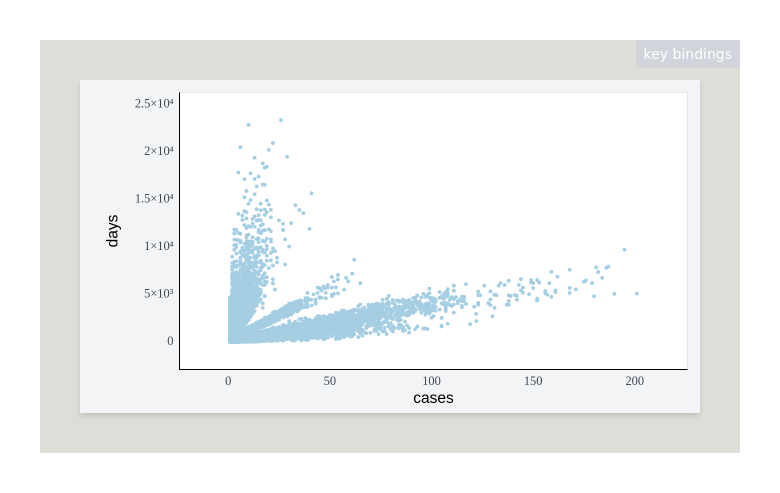
\includegraphics[width=1\linewidth,height=1\textheight]{./figures/example-cases-days} 

}

\caption{Relationship between the number of cases in a patient subgroup and the total number of days spent in care.}\label{fig:example-cases-days}
\end{figure}

Interestingly, the points did not show a simple linear trend. Instead, they seemed to cluster in three distinct ``leaflets'', each exhibiting a roughly linear trend. This suggests the presence of a pooling effect, such that the overall trend is the result of combining three distinct groups. Closer inspection of the data reveals that the \texttt{stay\_category} variable has three levels: short-term (\textless{} 3 months), medium-term (3-6 months), and long-term (6+ months) care. Color-coding the cases indeed confirms that the three levels of \texttt{stay\_category} correspond to the leaflets:

\begin{Shaded}
\begin{Highlighting}[]
\NormalTok{df }\SpecialCharTok{|\textgreater{}}
  \FunctionTok{create\_schema}\NormalTok{() }\SpecialCharTok{|\textgreater{}}
  \FunctionTok{add\_scatterplot}\NormalTok{(}\FunctionTok{c}\NormalTok{(}\StringTok{"cases"}\NormalTok{, }\StringTok{"days"}\NormalTok{)) }\SpecialCharTok{|\textgreater{}}
  \FunctionTok{add\_barplot}\NormalTok{(}\FunctionTok{c}\NormalTok{(}\StringTok{"stay\_category"}\NormalTok{, }\StringTok{"cases"}\NormalTok{)) }\SpecialCharTok{|\textgreater{}} \CommentTok{\# y{-}axis is weighted by cases}
  \FunctionTok{assign\_cases}\NormalTok{(}\FunctionTok{which}\NormalTok{(df}\SpecialCharTok{$}\NormalTok{stay\_category }\SpecialCharTok{==} \StringTok{"short"}\NormalTok{), }\DecValTok{1}\NormalTok{) }\SpecialCharTok{|\textgreater{}} \CommentTok{\# Mark short{-}term green}
  \FunctionTok{assign\_cases}\NormalTok{(}\FunctionTok{which}\NormalTok{(df}\SpecialCharTok{$}\NormalTok{stay\_category }\SpecialCharTok{==} \StringTok{"long"}\NormalTok{), }\DecValTok{2}\NormalTok{) }\SpecialCharTok{|\textgreater{}} \CommentTok{\# Mark long{-}term red}
  \FunctionTok{render}\NormalTok{()}
\end{Highlighting}
\end{Shaded}

\begin{figure}

{\centering \includegraphics[width=1\linewidth,height=1\textheight]{./figures/example-cases-stay-cat} 

}

\caption{The relationship between cases and days is subject to a pooling effect: while patient groups within each care duration category (short-term, medium-term, and long-term) exhibit a linear relationship individually, this does not hold when the groups are considered together.}\label{fig:example-cases-stay-cat}
\end{figure}

\begin{quote}
Click on the barplot bars to confirm there is a fairly minimal overlap between points belonging to the three categories (selected points will be brought to the foreground). To remove all selection, double-click the figure.
\end{quote}

However, the pooling effect does not itself explain the absence of points between the three leaflets. If the distribution of cases and days within each of the three \texttt{stay\_category} levels were uniform, we should expect to see more points in the gaps between the leaflets. This additionally suggests a potential selection process, where patients are less likely to be discharged at durations near the category boundaries. We can confirm this by plotting the average number of days spent in care:

\begin{Shaded}
\begin{Highlighting}[]
\CommentTok{\# Compute the average number of days spent in treatment}
\NormalTok{df}\SpecialCharTok{$}\NormalTok{avg\_days }\OtherTok{\textless{}{-}}\NormalTok{ df}\SpecialCharTok{$}\NormalTok{days }\SpecialCharTok{/}\NormalTok{ df}\SpecialCharTok{$}\NormalTok{cases }

\NormalTok{df }\SpecialCharTok{|\textgreater{}}  
  \FunctionTok{create\_schema}\NormalTok{() }\SpecialCharTok{|\textgreater{}}
  \FunctionTok{add\_scatterplot}\NormalTok{(}\FunctionTok{c}\NormalTok{(}\StringTok{"cases"}\NormalTok{, }\StringTok{"avg\_days"}\NormalTok{)) }\SpecialCharTok{|\textgreater{}}
  \FunctionTok{add\_barplot}\NormalTok{(}\FunctionTok{c}\NormalTok{(}\StringTok{"stay\_category"}\NormalTok{, }\StringTok{"cases"}\NormalTok{)) }\SpecialCharTok{|\textgreater{}}
  \FunctionTok{assign\_cases}\NormalTok{(}\FunctionTok{which}\NormalTok{(df}\SpecialCharTok{$}\NormalTok{stay\_category }\SpecialCharTok{==} \StringTok{"short{-}term"}\NormalTok{), }\DecValTok{1}\NormalTok{) }\SpecialCharTok{|\textgreater{}}
  \FunctionTok{assign\_cases}\NormalTok{(}\FunctionTok{which}\NormalTok{(df}\SpecialCharTok{$}\NormalTok{stay\_category }\SpecialCharTok{==} \StringTok{"long{-}term"}\NormalTok{), }\DecValTok{2}\NormalTok{) }\SpecialCharTok{|\textgreater{}}
  \FunctionTok{set\_scale}\NormalTok{(}\StringTok{"scatterplot1"}\NormalTok{, }\StringTok{"y"}\NormalTok{, }\CommentTok{\# Log{-}transform the y{-}axis}
            \AttributeTok{transformation =} \StringTok{"log10"}\NormalTok{, }\AttributeTok{default =} \ConstantTok{TRUE}\NormalTok{) }\SpecialCharTok{|\textgreater{}}
  \FunctionTok{render}\NormalTok{()}
\end{Highlighting}
\end{Shaded}

\begin{center}\includegraphics[width=1\linewidth,height=1\textheight]{./figures/example-cases-avg-days} \end{center}

Now we can clearly see the gaps between the three different distributions along the y-axis.

\begin{quote}
Try querying the points near the y-axis gaps by pressing the \texttt{Q} key and hovering over them. You should observe that the gaps roughly span the 60-90 day and 150-210 day ranges, corresponding to 2-3 months and 5-7 months, respectively.
\end{quote}

The trend we see in the scatterplot above strong indication of a selection process is at work. Specifically, it seems that patients who stay in treatment for more than two months are likely to be transferred to medium-term care and kept around for longer, and, likewise, those who stay in treatment for more than five months are likely to be moved to long-term care. There are likely administrative of health-insurance related reasons for this trend, nevertheless, it is still an interesting pattern to take note of.

\subsubsection{Number of cases over time}\label{number-of-cases-over-time}

A key question is how have the numbers of patients in treatment evolved over time. We can investigate this by plotting the same scatterplot as we did in the section above, as well as two barplots showing the total number of cases and the total number days in treatment, within each year. We can also include a histogram of the number of days, for a good measure:

\begin{Shaded}
\begin{Highlighting}[]
\NormalTok{schema }\OtherTok{\textless{}{-}}\NormalTok{ df }\SpecialCharTok{|\textgreater{}}
  \FunctionTok{create\_schema}\NormalTok{() }\SpecialCharTok{|\textgreater{}}
  \FunctionTok{add\_scatterplot}\NormalTok{(}\FunctionTok{c}\NormalTok{(}\StringTok{"cases"}\NormalTok{, }\StringTok{"days"}\NormalTok{)) }\SpecialCharTok{|\textgreater{}}
  \FunctionTok{add\_barplot}\NormalTok{(}\FunctionTok{c}\NormalTok{(}\StringTok{"year"}\NormalTok{, }\StringTok{"cases"}\NormalTok{)) }\SpecialCharTok{|\textgreater{}}
  \FunctionTok{add\_barplot}\NormalTok{(}\FunctionTok{c}\NormalTok{(}\StringTok{"year"}\NormalTok{, }\StringTok{"days"}\NormalTok{)) }\SpecialCharTok{|\textgreater{}}
  \FunctionTok{add\_histogram}\NormalTok{(}\FunctionTok{c}\NormalTok{(}\StringTok{"days"}\NormalTok{, }\StringTok{"days"}\NormalTok{)) }\SpecialCharTok{|\textgreater{}} \CommentTok{\# Again, make sure to weigh the y{-}axis}
  \FunctionTok{set\_parameters}\NormalTok{(}\StringTok{"histogram1"}\NormalTok{, }\AttributeTok{width =} \DecValTok{20}\NormalTok{) }\CommentTok{\# Set histogram binwidth to 20 days}

\NormalTok{schema }\SpecialCharTok{|\textgreater{}} \FunctionTok{render}\NormalTok{()}
\end{Highlighting}
\end{Shaded}

\begin{center}\includegraphics[width=1\linewidth,height=1\textheight]{./figures/example-cases-days-time} \end{center}

From the barplots, we can immediately see an interesting pattern: while the numbers of cases seem to have declined over time, the number of days patients spent in care seem to seems to have remained fairly constant. This suggest that while there are fewer patients over all, they are being hospitalized for longer.

We can confirm this interactively. Click on the bars corresponding to the year 2010 and 2022, in either of the two barplots (feel free to mark either of the bars by holding down the \texttt{1} or \texttt{2} keys and clicking them). You should see that, compared to 2010, there were more patients in long term care in 2022, and the relationship between the number of cases and the number of days in care was steeper.

On its own, the declining number of cases over time might appear as a positive development; however, the constant number days in treatment suggests a more worrying trend. Specifically, treatment facility placements are limited resource (\citeproc{ref-who2022}{Organization 2022}), and the fact that days in treatment have stayed constant while cases have declined may indicate that the Czech healthcare system is becoming burdened by patients in long-term care, reducing its capacity to serve new clients.

Another way we can scrutinize the trend more closely by zooming into the histogram:

\begin{Shaded}
\begin{Highlighting}[]
\NormalTok{schema }\SpecialCharTok{|\textgreater{}} 
  \FunctionTok{assign\_cases}\NormalTok{(}\FunctionTok{which}\NormalTok{(df}\SpecialCharTok{$}\NormalTok{year }\SpecialCharTok{==} \DecValTok{2010}\NormalTok{), }\DecValTok{1}\NormalTok{) }\SpecialCharTok{|\textgreater{}}
  \FunctionTok{assign\_cases}\NormalTok{(}\FunctionTok{which}\NormalTok{(df}\SpecialCharTok{$}\NormalTok{year }\SpecialCharTok{==} \DecValTok{2022}\NormalTok{), }\DecValTok{2}\NormalTok{) }\SpecialCharTok{|\textgreater{}}
  \FunctionTok{zoom}\NormalTok{(}\StringTok{"histogram1"}\NormalTok{, }\FunctionTok{c}\NormalTok{(}\SpecialCharTok{{-}}\DecValTok{100}\NormalTok{, }\DecValTok{0}\NormalTok{, }\FloatTok{3e03}\NormalTok{, }\FloatTok{1e05}\NormalTok{), }\AttributeTok{units =} \StringTok{"data"}\NormalTok{) }\SpecialCharTok{|\textgreater{}}
  \FunctionTok{render}\NormalTok{()}
\end{Highlighting}
\end{Shaded}

\begin{center}\includegraphics[width=1\linewidth,height=1\textheight]{./figures/example-cases-days-time-zoom} \end{center}

\begin{quote}
You can zoom into a plot in two ways: programmatically using the \texttt{zoom} function (as shown above), or manually by clicking and dragging to select a rectangular region and pressing the \texttt{Z} key. You can chain multiple zooms to magnify small regions of the plot. To undo zooming, press either the \texttt{X} to revert back one level of zoom, or \texttt{R} to reset the figure to its default state (including the default zoom level).
\end{quote}

By clicking on the two bars, you should be able to see that, compared to 2010, the 2022 distribution of days spent in treatment had a fatter tail, suggesting that there were more patients who spent very long time in care.

\subsubsection{Age and child and adolescent mental health}\label{age-and-child-and-adolescent-mental-health}

The global mental health decline affects adults and children alike, however, childhood mental health disorders are particularly concerning. If these disorders manifest during critical developmental periods, they can have serious, often life-long consequences, causing irreversible changes in brain physiology even with successful treatment (see e.g. \citeproc{ref-keeley2021}{Keeley 2021}). Children also have less agency than adults in managing their mental health, relying heavily on caregivers and schools for support. For these reasons and more, monitoring the mental health of children and adolescents is critical.

Fortunately, the overall proportion of children and adolescents in the data set was fairly low, amounting to \textless9\% of all cases and \textless6\% of the total number of days spent in treatment:

\begin{Shaded}
\begin{Highlighting}[]
\FunctionTok{aggregate}\NormalTok{(}\FunctionTok{cbind}\NormalTok{(cases, days) }\SpecialCharTok{\textasciitilde{}}\NormalTok{ care\_category, sum, }\AttributeTok{data =}\NormalTok{ df) }\SpecialCharTok{|\textgreater{}}
  \FunctionTok{lapply}\NormalTok{(}\ControlFlowTok{function}\NormalTok{(x) \{ }\ControlFlowTok{if}\NormalTok{ (}\FunctionTok{is.numeric}\NormalTok{(x)) }\FunctionTok{return}\NormalTok{(x }\SpecialCharTok{/} \FunctionTok{sum}\NormalTok{(x)) }\ControlFlowTok{else}\NormalTok{ x \}) }\SpecialCharTok{|\textgreater{}}
  \FunctionTok{data.frame}\NormalTok{()}
\end{Highlighting}
\end{Shaded}

\begin{verbatim}
##   care_category      cases       days
## 1         adult 0.91028915 0.94285172
## 2         child 0.08971085 0.05714828
\end{verbatim}

To investigate how these numbers evolved over time, we can make use of the following figure:

\begin{Shaded}
\begin{Highlighting}[]
\CommentTok{\# Create a figure layout with two small plots in the left}
\CommentTok{\# column, and one tall plot in the right column}
\NormalTok{layout }\OtherTok{\textless{}{-}} \FunctionTok{matrix}\NormalTok{(}\FunctionTok{c}\NormalTok{(}
  \DecValTok{1}\NormalTok{, }\DecValTok{3}\NormalTok{,}
  \DecValTok{2}\NormalTok{, }\DecValTok{3}
\NormalTok{), }\AttributeTok{nrow =} \DecValTok{2}\NormalTok{, }\AttributeTok{byrow =} \ConstantTok{TRUE}\NormalTok{)}

\NormalTok{df }\SpecialCharTok{|\textgreater{}}
  \FunctionTok{create\_schema}\NormalTok{() }\SpecialCharTok{|\textgreater{}}
  \FunctionTok{add\_barplot}\NormalTok{(}\FunctionTok{c}\NormalTok{(}\StringTok{"year"}\NormalTok{, }\StringTok{"cases"}\NormalTok{)) }\SpecialCharTok{|\textgreater{}}
  \FunctionTok{add\_barplot}\NormalTok{(}\FunctionTok{c}\NormalTok{(}\StringTok{"year"}\NormalTok{, }\StringTok{"days"}\NormalTok{)) }\SpecialCharTok{|\textgreater{}}
  \FunctionTok{add\_barplot}\NormalTok{(}\FunctionTok{c}\NormalTok{(}\StringTok{"care\_category"}\NormalTok{, }\StringTok{"cases"}\NormalTok{)) }\SpecialCharTok{|\textgreater{}}
  \FunctionTok{set\_layout}\NormalTok{(layout) }\SpecialCharTok{|\textgreater{}} \CommentTok{\# Set the layout}
  \FunctionTok{render}\NormalTok{() }
\end{Highlighting}
\end{Shaded}

\begin{center}\includegraphics[width=1\linewidth,height=1\textheight]{./figures/example-cases-days-children} \end{center}

So far, we have been using a fairly simple interactive workflow that could be easily recreated via code, taking only one or two interactive actions at a time. However, now it is time to see the full potential of interactivity by chaining several interactive actions together. To explore how the proportion of child and adolescent patients evolved over time, try taking the following steps:

\begin{quote}
\begin{enumerate}
\def\labelenumi{\arabic{enumi}.}
\tightlist
\item
  Mark the cases corresponding to children: click on the corresponding bar in the right barplot while holding down the \texttt{1} key.
\item
  Normalize the two leftmost barplots: click each of on the plots to activate it and press the \texttt{N} key while the plot is active (you can revert back to absolute counts by pressing the \texttt{N} key again).
\item
  Zoom into the regions of the leftmost barplots containing selected cases: click-and-drag to select a rectangular region and pressing the \texttt{Z} key.
\end{enumerate}
\end{quote}

By following these steps, you should end up with a figure similar to the one below:

\begin{Shaded}
\begin{Highlighting}[]
\NormalTok{df }\SpecialCharTok{|\textgreater{}}
  \FunctionTok{create\_schema}\NormalTok{() }\SpecialCharTok{|\textgreater{}}
  \FunctionTok{add\_barplot}\NormalTok{(}\FunctionTok{c}\NormalTok{(}\StringTok{"year"}\NormalTok{, }\StringTok{"cases"}\NormalTok{)) }\SpecialCharTok{|\textgreater{}}
  \FunctionTok{add\_barplot}\NormalTok{(}\FunctionTok{c}\NormalTok{(}\StringTok{"year"}\NormalTok{, }\StringTok{"days"}\NormalTok{)) }\SpecialCharTok{|\textgreater{}}
  \FunctionTok{add\_barplot}\NormalTok{(}\FunctionTok{c}\NormalTok{(}\StringTok{"care\_category"}\NormalTok{, }\StringTok{"cases"}\NormalTok{)) }\SpecialCharTok{|\textgreater{}}
  \FunctionTok{assign\_cases}\NormalTok{(}\FunctionTok{which}\NormalTok{(df}\SpecialCharTok{$}\NormalTok{care\_category }\SpecialCharTok{==} \StringTok{"child"}\NormalTok{)) }\SpecialCharTok{|\textgreater{}}
\NormalTok{  plotscaper}\SpecialCharTok{::}\FunctionTok{normalize}\NormalTok{(}\StringTok{"barplot1"}\NormalTok{) }\SpecialCharTok{|\textgreater{}}
\NormalTok{  plotscaper}\SpecialCharTok{::}\FunctionTok{normalize}\NormalTok{(}\StringTok{"barplot2"}\NormalTok{) }\SpecialCharTok{|\textgreater{}}
  \FunctionTok{zoom}\NormalTok{(}\StringTok{"barplot1"}\NormalTok{, }\FunctionTok{c}\NormalTok{(}\DecValTok{0}\NormalTok{, }\DecValTok{0}\NormalTok{, }\DecValTok{1}\NormalTok{, }\FloatTok{0.15}\NormalTok{)) }\SpecialCharTok{|\textgreater{}}
  \FunctionTok{zoom}\NormalTok{(}\StringTok{"barplot2"}\NormalTok{, }\FunctionTok{c}\NormalTok{(}\DecValTok{0}\NormalTok{, }\DecValTok{0}\NormalTok{, }\DecValTok{1}\NormalTok{, }\FloatTok{0.15}\NormalTok{)) }\SpecialCharTok{|\textgreater{}}
  \FunctionTok{set\_layout}\NormalTok{(layout) }\SpecialCharTok{|\textgreater{}}
  \FunctionTok{render}\NormalTok{() }
\end{Highlighting}
\end{Shaded}

\begin{figure}

{\centering \includegraphics[width=1\linewidth,height=1\textheight]{./figures/example-cases-days-children-marked} 

}

\caption{While the proportion of days spent in treatment by children and adolescent has declined, the proportion of cases that children and adolescents make up has increased.}\label{fig:example-cases-days-children-marked}
\end{figure}

Interestingly, the two barplots show the opposite trend. While the proportion of the treatment days used by children and adolescents has declined over time, the proportion of total cases they make up has increased. The relative increase in cases appears to be driven by an overall decline in patient numbers: in absolute counts, the number of child and adolescent patients has remained fairly constant between 2010 to 2022, while the total patient count has decreased.

We can also get a more granular breakdown by plotting the age category variable:

\begin{Shaded}
\begin{Highlighting}[]
\NormalTok{df }\SpecialCharTok{|\textgreater{}}
  \FunctionTok{create\_schema}\NormalTok{() }\SpecialCharTok{|\textgreater{}}
  \FunctionTok{add\_barplot}\NormalTok{(}\FunctionTok{c}\NormalTok{(}\StringTok{"age\_category"}\NormalTok{, }\StringTok{"cases"}\NormalTok{)) }\SpecialCharTok{|\textgreater{}}
  \FunctionTok{add\_barplot}\NormalTok{(}\FunctionTok{c}\NormalTok{(}\StringTok{"year"}\NormalTok{, }\StringTok{"cases"}\NormalTok{)) }\SpecialCharTok{|\textgreater{}}
  \FunctionTok{add\_barplot}\NormalTok{(}\FunctionTok{c}\NormalTok{(}\StringTok{"age\_category"}\NormalTok{, }\StringTok{"days"}\NormalTok{)) }\SpecialCharTok{|\textgreater{}}
  \FunctionTok{add\_barplot}\NormalTok{(}\FunctionTok{c}\NormalTok{(}\StringTok{"year"}\NormalTok{, }\StringTok{"days"}\NormalTok{)) }\SpecialCharTok{|\textgreater{}}
  \FunctionTok{render}\NormalTok{()}
\end{Highlighting}
\end{Shaded}

\begin{center}\includegraphics[width=1\linewidth,height=1\textheight]{./figures/example-cases-days-age} \end{center}

Again, if we interrogate the figure by employing interactive actions such as selection, zooming, and normalization, we can discover that one age category in which there has been steady growth in both the proportion of cases and days spend in treatment are 70-79 year olds. This aligns with the limited placement availability hypothesis: while these patients account for a relatively small fraction of the total cases, they represent a disproportionately large and increasing proportion of days in treatment. Later, we will also see evidence that many of these patients suffer from neurodegenerative diseases, which require intensive long-term care. It may be the case that, with increasing life-expectancy, the healthcare system is not able to handle the influx of older patients, limiting the availability of placements.

\subsubsection{Prevalence of diagnoses}\label{prevalence-of-diagnoses}

Another important information we can glean from the data set is the prevalence of different diagnoses and their demographic characteristics. The data set identifies mental disorders according to ICD-10, an internationally recognized disease classification system published by the World Health organization which organizes various diseases into categories based on aetiology (\citeproc{ref-icd2024a}{World Health Organization 2024a}).

It is first necessary to discuss the coding scheme of the diagnoses. The codes were directly translated from the Czech version of the data set (\citeproc{ref-soukupova2023}{Soukupová et al. 2023}). The vast majority diagnoses come from the F category, which represents mental and behavioral disorders, although there are also few references to the G category, which classifies diseases of the nervous system. Further, note that while some levels of the \texttt{diagnosis} variable represent a singular ICD-10 diagnosis (e.g.~\texttt{f10}), others represent a range of diagnoses (e.g.~\texttt{f11-f19}), a union (e.g.~\texttt{f0\ and\ g30}), or an exclusive difference (e.g.~\texttt{f4\ without\ f42}).

Importantly, some of the codes also represent a range of diagnoses \emph{implicitly}. For instance, whereas \texttt{f10} code refers to the F10 diagnosis (alcohol-use disorders), the part \texttt{f4} in \texttt{f4\ without\ f42} does \emph{not} refer to the F04 diagnosis (organic amnesic syndrome, not induced by alcohol and other psychoactive substances) but instead to the F40-F48 range of diagnoses (neurotic, stress-related and somatoform disorders, \citeproc{ref-icd2024a}{World Health Organization 2024a}). Likewise, \texttt{f2} represents F20-F29 (schizophrenia, schizotypal and delusional disorders), \texttt{f7} represents F70-F79 (mental retardation), and \texttt{f5} represents F50-F59 (behavioural syndromes associated with physiological disturbances and physical factors). I have confirmed this via personal communication with the data set's authors (\citeproc{ref-melicharova2025}{Melicharová 2025}).

Table \ref{tab:icd10} lists codes used in the data, in order of their prevalence (the number of all cases across all time), along with a short description based on the ICD-10 (\citeproc{ref-icd2024a}{World Health Organization 2024a}), and some clarifying notes in parentheses that I myself have added:

\begin{table}
\centering
\caption{\label{tab:icd10}The data diagnosis code and ICD-10 description}
\centering
\begin{tabular}[t]{l|l}
\hline
Code & Description\\
\hline
f10 & Mental and behavioural disorders due to use of alcohol\\
\hline
f2 & Schizophrenia, schizotypal and delusional disorders (f20-f29)\\
\hline
f0 and g30 & Dementia in Alzheimer’s disease (f0), Alzheimer’s disease (g30)\\
\hline
f4 without f42 & Neurotic, stress-related and somatoform disorders (f40-f48; includes e.g. specific phobias, generalized anxiety disorder, and post-traumatic stress disorder), without obsessive-compulsive disorder (f42)\\
\hline
f11-f19 & Mental and behavioural disorders due to psychoactive substance use (excluding alcohol use, f10)\\
\hline
f8–f9 & Disorders of psychological development (f80-f89), behavioural and emotional disorders with onset usually occurring in childhood and adolescence (f90-f98) and unspecified mental disorder (f99)\\
\hline
f32–f33 & Depressive episode (f32), recurrent depressive disorder (f33)\\
\hline
f60–f61 & Specific personality disorders (f60; includes e.g. paranoid, schizoid, histrionic, or anxious/avoidant personality disorders), mixed and other personality disorders (f61)\\
\hline
f7 & Mental retardation (f70-f79)\\
\hline
f3 without f32 \& f33 & Mood [affective] disorders (f30-f39) without depressive episode (f32) and recurrent depressive disorder (f33)\\
\hline
f62–f69 & Personality and behavioral disorders (includes things such as PTSD, habit and impulse disorders, sexual preference disorders, etc...)\\
\hline
f5 & Behavioural syndromes associated with physiological disturbances and physical factors (f50-f59; includes eating disorders, sleep disorders, sexual dysfunction disorders, and others)\\
\hline
other & \\
\hline
f42 & Obsessive-compulsive disorder\\
\hline
\end{tabular}
\end{table}

To explore the prevalence of the various diagnoses as well as their demographic characteristics, we create another interactive figure. For this figure, I decided to plot the following variables: \texttt{diagnosis}, \texttt{age\_category}, \texttt{sex}, and \texttt{reason\_for\_termination}. These seemed like the most interesting demographic variables. The \texttt{region} variable could also be an interesting choice, however, initial exploration did not reveal any interesting trends so I decided to omit it.

From now on, I will describe interesting features of the data in text rather than through individual figures. You are encouraged to verify these findings by interacting with the figures and using the techniques discussed so far.

\begin{Shaded}
\begin{Highlighting}[]
\CommentTok{\# Create ordering for barplots based on frequency}
\NormalTok{order\_df }\OtherTok{\textless{}{-}} \FunctionTok{aggregate}\NormalTok{(cases }\SpecialCharTok{\textasciitilde{}}\NormalTok{ diagnosis, sum, }\AttributeTok{data =}\NormalTok{ df)}
\NormalTok{order\_df }\OtherTok{\textless{}{-}}\NormalTok{ order\_df[}\FunctionTok{order}\NormalTok{(order\_df}\SpecialCharTok{$}\NormalTok{cases), ]}

\NormalTok{order\_df2 }\OtherTok{\textless{}{-}} \FunctionTok{aggregate}\NormalTok{(cases }\SpecialCharTok{\textasciitilde{}}\NormalTok{ reason\_for\_termination, sum, }\AttributeTok{data =}\NormalTok{ df)}
\NormalTok{order\_df2 }\OtherTok{\textless{}{-}}\NormalTok{ order\_df2[}\FunctionTok{order}\NormalTok{(order\_df2}\SpecialCharTok{$}\NormalTok{cases), ]}

\NormalTok{df }\SpecialCharTok{|\textgreater{}}
  \FunctionTok{create\_schema}\NormalTok{() }\SpecialCharTok{|\textgreater{}}
  \FunctionTok{add\_barplot}\NormalTok{(}\FunctionTok{c}\NormalTok{(}\StringTok{"diagnosis"}\NormalTok{, }\StringTok{"cases"}\NormalTok{)) }\SpecialCharTok{|\textgreater{}}
  \FunctionTok{add\_barplot}\NormalTok{(}\FunctionTok{c}\NormalTok{(}\StringTok{"age\_category"}\NormalTok{, }\StringTok{"cases"}\NormalTok{)) }\SpecialCharTok{|\textgreater{}}
  \FunctionTok{add\_barplot}\NormalTok{(}\FunctionTok{c}\NormalTok{(}\StringTok{"sex"}\NormalTok{, }\StringTok{"cases"}\NormalTok{)) }\SpecialCharTok{|\textgreater{}}
  \FunctionTok{add\_barplot}\NormalTok{(}\FunctionTok{c}\NormalTok{(}\StringTok{"reason\_for\_termination"}\NormalTok{, }\StringTok{"cases"}\NormalTok{)) }\SpecialCharTok{|\textgreater{}}
  \CommentTok{\# Sort the bars by prevalence (can also do interactively by pressing \textasciigrave{}O\textasciigrave{} key)}
  \FunctionTok{set\_scale}\NormalTok{(}\StringTok{"barplot1"}\NormalTok{, }\StringTok{"x"}\NormalTok{, }\AttributeTok{breaks =}\NormalTok{ order\_df}\SpecialCharTok{$}\NormalTok{diagnosis) }\SpecialCharTok{|\textgreater{}} 
  \FunctionTok{set\_scale}\NormalTok{(}\StringTok{"barplot4"}\NormalTok{, }\StringTok{"x"}\NormalTok{, }\AttributeTok{breaks =}\NormalTok{ order\_df2}\SpecialCharTok{$}\NormalTok{reason\_for\_termination) }\SpecialCharTok{|\textgreater{}} 
  \FunctionTok{render}\NormalTok{()}
\end{Highlighting}
\end{Shaded}

\begin{figure}

{\centering \includegraphics[width=1\linewidth,height=1\textheight]{./figures/example-cases-diagnosis} 

}

\caption{Majority of patient load was taken up by the top five most common disorders: alcohol-use disorders, schizophrenia, Alzheimer's disease, neurotic and stress-related disorders, and psychoactive substance disorders.}\label{fig:example-cases-diagnosis}
\end{figure}

The barplot in the top left panel of the Figure \ref{fig:example-cases-diagnosis} shows that the five most common disorders accounted for the majority of patient cases. Each of these disorders affected over 40,000 patients between 2010 and 2022, representing over 75\% of all cases (319,557 out of 414,242).

\begin{quote}
Press the \texttt{Q} key and hover over the bars in the top left panel of Figure \ref{fig:example-cases-diagnosis} to see what diagnosis each represents.
\end{quote}

In order of prevalence, the top five disorders were, were: alcohol-use disorders, schizophrenia, Alzheimer's disease, neurotic and stress-related disorders, and disorders caused by psychoactive substances (excluding alcohol). Overall, the high prevalence of these disorders is fairly, given that their high socio-economic impact is well-known to psychiatrists. Nevertheless, it may be illustrative to take a closer look at this data and examine demographic trends.

First, alcohol use disorders were the most common diagnosis. This is not surprising, since, globally, alcohol use disorders rank among the most common disorders and are associated with high mortality due to chronic health conditions and injury (\citeproc{ref-carvalho2019}{Carvalho et al. 2019}). In the data set, this diagnosis was about twice as common in men and showed a fairly symmetric, normal-shaped age distribution, occurring the most frequently in 40-49 and 50-59 year-olds (this can be seen by selecting the corresponding bar in the top-left panel of figure Figure \ref{fig:example-cases-diagnosis} and normalizing the age-category barplot).

The second most prevalent category of diagnoses were schizophrenia, schizotypal, and delusional disorders. While the individual lifetime prevalence of schizophrenia is not as high as some other disorders on this list, the reason for its high representation in the data set is likely its chronic and serious nature. Among those with mental illness, people with schizophrenia have one of the lowest life expectancies (see e.g. \citeproc{ref-chang2011}{C.-K. Chang et al. 2011}), and often require multi-year or even life-long hospitalization (\citeproc{ref-messias2007}{Messias, Chen, and Eaton 2007}). This debilitating nature of schizophrenia has prompted some experts to describe it as ``arguably one of the most severe health conditions affecting mankind'' (see e.g. \citeproc{ref-messias2007}{Messias, Chen, and Eaton 2007}; \citeproc{ref-tandon2024}{Tandon et al. 2024}). In the data set at hand, schizophrenic disorders had a fairly balanced sex ratio and a fairly flat age distribution.

Third most prevalent disorder categories was Alzheimer's disease. The high prevalence of this disorder is unfortunately also to be expected, as, in developed countries, Alzheimer's disease tends the leading cause of long-term psychiatric care in old age (see e.g. \citeproc{ref-cao2020}{Cao et al. 2020}; \citeproc{ref-langa2017}{Langa et al. 2017}). It also tends to be more prevalent in women. These patterns could be seen fairly well in the data set: the age distribution of Alzheimer's disease was strongly skewed, occurring much more frequently in older patients (and, in fact, making up the majority of \textgreater70 year-old patients), and the diagnosis was about \textasciitilde40\% more prevalent in women than in men. We can also see that Alzheimer's patient made up the vast majority of patients who had died in care, further reinforcing its status as a disease of old age.

The fourth most prevalent category of disorders were neurotic, stress-related, and somatoform disorders (excluding the obsessive-compulsive disorder, F42) which was classified as its own category in the data set. This category includes disorders such as specific phobias, generalized anxiety disorder, and the post-traumatic stress disorder (\citeproc{ref-icd2024a}{World Health Organization 2024a}). These disorders are known to be relatively common, occur roughly twice as often in women as in men, and have a generally even age distribution, with decline in prevalence in older age (\citeproc{ref-bandelow2015}{Bandelow and Michaelis 2015}). This pattern could be seen well in the data set, with women making up the majority of the cases and the age distribution being fairly uniform, until a drop-off starting at about 60-69 years of age. In fact, these disorders were the most common diagnosis for women under 40:

\begin{Shaded}
\begin{Highlighting}[]
\NormalTok{df}\SpecialCharTok{$}\NormalTok{age\_category\_n }\OtherTok{\textless{}{-}} \FunctionTok{as.numeric}\NormalTok{(}\FunctionTok{factor}\NormalTok{(df}\SpecialCharTok{$}\NormalTok{age\_category, }\AttributeTok{ordered =} \ConstantTok{TRUE}\NormalTok{))}
\NormalTok{under\_40 }\OtherTok{\textless{}{-}} \FunctionTok{unique}\NormalTok{(df}\SpecialCharTok{$}\NormalTok{age\_category\_n[df}\SpecialCharTok{$}\NormalTok{age\_category }\SpecialCharTok{==} \StringTok{"30–39"}\NormalTok{])}

\FunctionTok{subset}\NormalTok{(df, sex }\SpecialCharTok{==} \StringTok{"female"} \SpecialCharTok{\&}\NormalTok{ age\_category\_n }\SpecialCharTok{\textless{}=}\NormalTok{ under\_40) }\SpecialCharTok{|\textgreater{}}
\NormalTok{  (\textbackslash{}(x) }\FunctionTok{aggregate}\NormalTok{(cases }\SpecialCharTok{\textasciitilde{}}\NormalTok{ diagnosis, sum, }\AttributeTok{data =}\NormalTok{ x))() }\SpecialCharTok{|\textgreater{}}
\NormalTok{  (\textbackslash{}(x) x[}\FunctionTok{order}\NormalTok{(}\SpecialCharTok{{-}}\NormalTok{x}\SpecialCharTok{$}\NormalTok{cases), ])() }\SpecialCharTok{|\textgreater{}}
  \FunctionTok{head}\NormalTok{(}\DecValTok{5}\NormalTok{) }\SpecialCharTok{|\textgreater{}}\NormalTok{ knitr}\SpecialCharTok{::}\FunctionTok{kable}\NormalTok{(}\AttributeTok{align =} \StringTok{"ll"}\NormalTok{, }\AttributeTok{row.names =} \ConstantTok{FALSE}\NormalTok{)}
\end{Highlighting}
\end{Shaded}

\begin{tabular}{l|l}
\hline
diagnosis & cases\\
\hline
f4 without f42 & 12599\\
\hline
f2 & 11783\\
\hline
f11–f19 & 10722\\
\hline
f8–f9 & 6882\\
\hline
f10 & 6880\\
\hline
\end{tabular}

The fifth and final of the top five diagnoses were disorders due to use of psychoactive substances. This finding is also not particularly surprising, since, among European countries, Czechia ranks moderately high in consumption psychoactive substances, particularly ecstasy and cannabis (\citeproc{ref-mounteney2016}{Mounteney et al. 2016}). By contrast to some of the earlier categories, this diagnosis was significantly more common in males and in young people, showing a skewed age distribution with peak in the 20-29 category. Interestingly, the patients in this category also made up a fairly high proportion of those who had their care terminated early. It is hard to say what this means exactly (a more detailed coding schema for this variable is not available), however, other disorders with high proportion of early terminations included personality disorders (F60-F61 and F62-F69), suggesting that perhaps some patients may be released from care early because of serious behavioral problems.

Overall, the high prevalence of the top five diagnoses seemed to stem from their broad scope which encompassed a wide range of disorders. For instance, alcohol and other psychoactive substance use disorders can manifest in diverse symptoms, including dependence, psychosis, and amnesic syndrome (\citeproc{ref-icd2024a}{World Health Organization 2024a}). Similarly, as was mentioned above, the stress-related diagnosis covers a broad spectrum of conditions. Alzheimer's disease was one notable exception, representing a fairly specific diagnosis with well-established physiological markers such as the presence of amyloid plaques and neurofibrillary tangles (see e.g. \citeproc{ref-deture2019}{DeTure and Dickson 2019}). It could be the case that, under a different classification scheme, Alzheimer's disease would be the most prevalent disorder.

Regardless, the diagnoses which followed the top five tended to be more specific, generally encompassing only one or two ICD-10 codes. Such was the case, for example, for depressive episode and recurrent depressive disorder (F32-F33), specific and mixed personality disorders (F60-F61), and so on. While it could be the case that these disorders would rank higher if some of the top five diagnoses were more granular as well, it is also possible that these disorders require less long-term care due to being more amenable to outpatient treatment methods (see e.g. \citeproc{ref-roiser2012}{Roiser, Elliott, and Sahakian 2012}).

\subsubsection{Prevalence of diagnoses over time}\label{prevalence-of-diagnoses-over-time}

We can also scrutinize the prevalence of different mental disorders over time. Again, we need to distinguish between the number of cases versus the number of days patients spent in care. We can use the following figure:

\begin{Shaded}
\begin{Highlighting}[]
\NormalTok{df }\SpecialCharTok{|\textgreater{}}
  \FunctionTok{create\_schema}\NormalTok{() }\SpecialCharTok{|\textgreater{}}
  \FunctionTok{add\_barplot}\NormalTok{(}\FunctionTok{c}\NormalTok{(}\StringTok{"diagnosis"}\NormalTok{, }\StringTok{"cases"}\NormalTok{)) }\SpecialCharTok{|\textgreater{}}
  \FunctionTok{add\_barplot}\NormalTok{(}\FunctionTok{c}\NormalTok{(}\StringTok{"year"}\NormalTok{, }\StringTok{"cases"}\NormalTok{)) }\SpecialCharTok{|\textgreater{}}
  \FunctionTok{add\_barplot}\NormalTok{(}\FunctionTok{c}\NormalTok{(}\StringTok{"year"}\NormalTok{, }\StringTok{"days"}\NormalTok{)) }\SpecialCharTok{|\textgreater{}}
  \FunctionTok{set\_layout}\NormalTok{(}\FunctionTok{matrix}\NormalTok{(}\FunctionTok{c}\NormalTok{(}\DecValTok{1}\NormalTok{, }\DecValTok{1}\NormalTok{, }\DecValTok{2}\NormalTok{, }\DecValTok{3}\NormalTok{), }\AttributeTok{nrow =} \DecValTok{2}\NormalTok{, }\AttributeTok{byrow =} \ConstantTok{TRUE}\NormalTok{)) }\SpecialCharTok{|\textgreater{}}
  \FunctionTok{set\_scale}\NormalTok{(}\StringTok{"barplot1"}\NormalTok{, }\StringTok{"x"}\NormalTok{, }\AttributeTok{breaks =}\NormalTok{ order\_df}\SpecialCharTok{$}\NormalTok{diagnosis) }\SpecialCharTok{|\textgreater{}}
  \FunctionTok{render}\NormalTok{()}
\end{Highlighting}
\end{Shaded}

\begin{center}\includegraphics[width=1\linewidth,height=1\textheight]{./figures/example-cases-diagnosis-time} \end{center}

Overall, over time, the proportion of both cases and days in treatment the various diagnoses made up seemed to remain fairly constant, with perhaps a slight general decreasing trend in the number of cases. Of the top five diagnoses, the one which seemed to buck this trend was schizophrenia (F20-F29), which had a fairly marked increasing trend in the proportion of days. Furthermore, the number of cases related to psychoactive substance use disorders (excluding alcohol) seemed to also be rising slightly.

Of the rarer disorders, the one in which there seemed to be a significant relative rise in both the proportion of cases and days in treatment were mental and behavioral disorders associated with physiological disturbances and physical factors (F50-F59). This category includes disorders such as anorexia, bulimia, sleep disorders, and sexual dysfunction disorders. Given that this category was more prevalent in women and young people (as can be seen by interrogating Figure \ref{fig:example-cases-diagnosis}), the likely explanation for this trend is rise in the number of cases of anorexia and bulimia. There also seemed to be slight of a decrease in the number of days spent in treatment by patients with stress-related disorders (F40-F49 without F42) and depression disorders (F32 and F33).

We can quickly verify these findings by fitting simple linear regressions for each diagnosis. First, we can model the number of cases by year:

\begin{table}
\centering
\caption{\label{tab:cases-by-year}Simple linear regressions of the number of cases by year for each diagnosis}
\centering
\begin{tabular}[t]{l|>{}l|>{}l|>{}l|l}
\hline
diagnosis & beta & lower 95\% CI & upper 95\% CI & p-value\\
\hline
f10 & \textcolor{red}{-0.09} & \textcolor{red}{-0.16} & \textcolor{red}{-0.02} & 0.01\\
\hline
f2 & \textcolor{red}{-0.26} & \textcolor{red}{-0.34} & \textcolor{red}{-0.19} & < 0.001\\
\hline
f0 and g30 & \textcolor{red}{-0.12} & \textcolor{red}{-0.19} & \textcolor{red}{-0.05} & < 0.001\\
\hline
f4 without f42 & \textcolor{red}{-0.26} & \textcolor{red}{-0.35} & \textcolor{red}{-0.17} & < 0.001\\
\hline
f11–f19 & \textcolor{red}{-0.08} & \textcolor{red}{-0.14} & \textcolor{red}{-0.02} & 0.014\\
\hline
f8–f9 & \textcolor{black}{0.14} & \textcolor{red}{-0.22} & \textcolor{black}{0.49} & 0.449\\
\hline
f32–f33 & \textcolor{red}{-0.11} & \textcolor{red}{-0.15} & \textcolor{red}{-0.07} & < 0.001\\
\hline
f60–f61 & \textcolor{red}{-0.13} & \textcolor{red}{-0.18} & \textcolor{red}{-0.09} & < 0.001\\
\hline
f7 & \textcolor{red}{-0.10} & \textcolor{red}{-0.15} & \textcolor{red}{-0.05} & < 0.001\\
\hline
f3 without f32\&f33 & \textcolor{red}{-0.07} & \textcolor{red}{-0.10} & \textcolor{red}{-0.04} & < 0.001\\
\hline
f62–f69 & \textcolor{red}{-0.09} & \textcolor{red}{-0.12} & \textcolor{red}{-0.06} & < 0.001\\
\hline
f5 & \textcolor{black}{0.11} & \textcolor{black}{0.04} & \textcolor{black}{0.17} & 0.001\\
\hline
other & \textcolor{red}{-0.02} & \textcolor{red}{-0.04} & \textcolor{red}{-0.01} & < 0.001\\
\hline
f42 & \textcolor{black}{0.01} & \textcolor{black}{0.00} & \textcolor{black}{0.03} & 0.127\\
\hline
\end{tabular}
\end{table}

As we can see in Table \ref{tab:prevalence-over-time}, for most diagnoses, there seemed to be a decreasing trend in the number of cases over time. The only diagnosis for which the number of cases was significantly \emph{increasing} over time was F50-F59, confirming the observations made in the interactive figure.

We can do the same for the number of days by year:

\begin{table}
\centering
\caption{\label{tab:days-by-year}Simple linear regressions of the number of days by year for each diagnosis}
\centering
\begin{tabular}[t]{l|>{}l|>{}l|>{}l|l}
\hline
diagnosis & beta & lower 95\% CI & upper 95\% CI & p-value\\
\hline
f10 & \textcolor{black}{5.02} & \textcolor{black}{1.16} & \textcolor{black}{8.88} & 0.011\\
\hline
f2 & \textcolor{black}{41.70} & \textcolor{black}{32.02} & \textcolor{black}{51.39} & < 0.001\\
\hline
f0 and g30 & \textcolor{black}{27.48} & \textcolor{black}{19.94} & \textcolor{black}{35.02} & < 0.001\\
\hline
f4 without f42 & \textcolor{red}{-3.79} & \textcolor{red}{-6.44} & \textcolor{red}{-1.14} & 0.005\\
\hline
f11–f19 & \textcolor{black}{3.89} & \textcolor{black}{1.07} & \textcolor{black}{6.71} & 0.007\\
\hline
f8–f9 & \textcolor{black}{0.72} & \textcolor{red}{-17.25} & \textcolor{black}{18.69} & 0.937\\
\hline
f32–f33 & \textcolor{red}{-4.32} & \textcolor{red}{-6.41} & \textcolor{red}{-2.23} & < 0.001\\
\hline
f60–f61 & \textcolor{black}{1.00} & \textcolor{red}{-1.64} & \textcolor{black}{3.64} & 0.456\\
\hline
f7 & \textcolor{black}{21.70} & \textcolor{black}{15.50} & \textcolor{black}{27.89} & < 0.001\\
\hline
f3 without f32\&f33 & \textcolor{red}{-1.84} & \textcolor{red}{-4.08} & \textcolor{black}{0.40} & 0.107\\
\hline
f62–f69 & \textcolor{black}{26.18} & \textcolor{black}{19.37} & \textcolor{black}{32.99} & < 0.001\\
\hline
f5 & \textcolor{black}{6.40} & \textcolor{black}{3.32} & \textcolor{black}{9.47} & < 0.001\\
\hline
other & \textcolor{black}{16.54} & \textcolor{black}{9.69} & \textcolor{black}{23.40} & < 0.001\\
\hline
f42 & \textcolor{black}{3.23} & \textcolor{black}{0.19} & \textcolor{black}{6.26} & 0.037\\
\hline
\end{tabular}
\end{table}

Here, the situation was a bit more varied. For most diagnoses, the number of days patients spent in care seemed to increase, with particularly large increases being observed for schizophrenia (F20-F29), Alzheimer's disease (F02 and G30), mental retardation (F70-F79), and personality disorders (F62-F69). The two diagnosis for which the number of days in treatment actually decreased were, interestingly, stress-related disorders (F40-F49 without F42) and depression disorders (F32 and F33).

\subsubsection{Characteristics of patient cohorts over time}\label{characteristics-of-patient-cohorts-over-time}

One final things we are going to investigate are characteristics of patient cohorts. Specifically, given that each row of data represents one patient cohort within a given year, of a given sex, diagnosis, and so on, we can investigate whether there were any interesting patterns within the patient cohorts over time. One way we can do this is via the following figure:

\begin{Shaded}
\begin{Highlighting}[]
\NormalTok{df }\SpecialCharTok{|\textgreater{}}
  \FunctionTok{create\_schema}\NormalTok{() }\SpecialCharTok{|\textgreater{}}
  \FunctionTok{add\_barplot}\NormalTok{(}\FunctionTok{c}\NormalTok{(}\StringTok{"diagnosis"}\NormalTok{, }\StringTok{"cases"}\NormalTok{)) }\SpecialCharTok{|\textgreater{}}
  \FunctionTok{add\_barplot}\NormalTok{(}\FunctionTok{c}\NormalTok{(}\StringTok{"year"}\NormalTok{, }\StringTok{"cases"}\NormalTok{), }\FunctionTok{list}\NormalTok{(}\AttributeTok{reducer =} \StringTok{"max"}\NormalTok{)) }\SpecialCharTok{|\textgreater{}}
  \FunctionTok{add\_barplot}\NormalTok{(}\FunctionTok{c}\NormalTok{(}\StringTok{"year"}\NormalTok{, }\StringTok{"days"}\NormalTok{), }\FunctionTok{list}\NormalTok{(}\AttributeTok{reducer =} \StringTok{"max"}\NormalTok{)) }\SpecialCharTok{|\textgreater{}}
  \FunctionTok{set\_scale}\NormalTok{(}\StringTok{"barplot1"}\NormalTok{, }\StringTok{"x"}\NormalTok{, }\AttributeTok{breaks =}\NormalTok{ order\_df}\SpecialCharTok{$}\NormalTok{diagnosis) }\SpecialCharTok{|\textgreater{}}
  \FunctionTok{set\_layout}\NormalTok{(}\FunctionTok{matrix}\NormalTok{(}\FunctionTok{c}\NormalTok{(}\DecValTok{1}\NormalTok{, }\DecValTok{1}\NormalTok{, }\DecValTok{2}\NormalTok{, }\DecValTok{3}\NormalTok{), }\AttributeTok{nrow =} \DecValTok{2}\NormalTok{)) }\SpecialCharTok{|\textgreater{}}
  \FunctionTok{render}\NormalTok{()}
\end{Highlighting}
\end{Shaded}

\begin{figure}

{\centering \includegraphics[width=1\linewidth,height=1\textheight]{./figures/example-cases-diagnosis-max} 

}

\caption{While Alzheimer's patients accounted for the longest hospitalized cohorts prior to 2016, following 2016, the longest hospitalized cohorts tended to be schizophrenia patients.}\label{fig:example-cases-diagnosis-max}
\end{figure}

In Figure \ref{fig:example-cases-diagnosis-max}, I show plots of diagnoses, as well as a summary of days and cases over time. However, note that, whereas all barplots of days and cases over time shown before had sum (of cases and days) as the y-axis summary statistic, the two barplots in the lower half of figure Figure \ref{fig:example-cases-diagnosis-max} show maximum, not sum. These plots effectively tell us the size and the number of days in treatment for the largest/longest hospitalized patient cohort within a given year. Based on theory in Section \ref{problems}, we know that these plots will behave well under linked selection (with one selection group).

By investigating the diagnoses, we can discover some interesting trends in the patient cohorts. Specifically, by comparing the schizophrenia (F20-F29) and the Alzheimer's disease diagnoses (F0 and G30), we can see that they show a complementary trend in the maximum number of days hospitalized. Specifically, whereas Alzheimer's disease generally accounted for the longest-hospitalized patient cohorts up until 2016, schizophrenia accounted for the longest-hospitalized patient cohorts for five of the six years following 2016 (excluding 2020, where Alzheimer's disease narrowly beat it out). This occurred despite schizophrenia patient cohorts shrinking in size over time and the fact that Alzheimer's disease was more restricted in terms of age-range, so we would naturally expect larger cohorts (due to ``lumping''). On that note, developmental disorders (F80-F99), despite the making up only a small proportion of the total number cases, made up many of the largest patients cohorts year over year. This is understandable given that these patients came almost exclusively from the youngest age group and were otherwise relatively homogeneous.

\section{Summary}\label{summary}

I have used the Long-term Care data set (\citeproc{ref-soukupova2023}{Soukupová et al. 2023}) to demonstrate the typical data analytic workflow using \texttt{plotscaper}. By creating interactive figures and leveraging a suite of interactive features such as linked selection, representation switching, querying, and zooming and panning, we were able to quickly discover many interesting features about the data set, highlighting the usefulness of the package and interactive data visualization in general.

Some key take-away points were:

\begin{itemize}
\tightlist
\item
  Since 2010, the number of cases has generally decreased, while the number of treatment days has remained constant, suggesting that fewer individuals are receiving long-term psychiatric care, but for longer durations. This suggests a limited placement availability hypothesis, where the healthcare system may be struggling to accommodate new patients due to existing patient load.
\item
  The trend of decreasing number of cases and increasing number of days was reversed for children, who represented a growing proportion of patients but a smaller proportion of treatment days over time.
\item
  The proportion of treatment days represented by older patients (60-69 and 70-79 year olds) has increased over time, further supporting the limited placement hypothesis, since these patients often require longer care.
\item
  There were few patients staying in care for periods of between 2-3 months and 5-7 months, suggesting that there may be potential selection mechanisms influencing hospitalization duration (e.g.~administrative reasons).
\item
  The five most common diagnoses were, in order: alcohol use disorders, schizophrenia, Alzheimer's disease, stress-related disorders, and psychoactive substance use disorders. Patient demographics for these disorders showed some very strong trends which largely aligned with the existing literature.
\item
  One diagnostic category which actually shown a significant increase in the number of cases over time were behavioural syndromes associated with physiological disturbances and physical factors. Given that this category includes disorders like anorexia and bulimia, and that the majority of cases were young women, this suggests that, while rare, eating disorders may be on the rise, and should be given attention.
\item
  While initially, the longest hospitalized patient cohorts tended to be Alzheimer's patients, over time, schizophrenia patients became the longest hospitalized patient cohorts
\end{itemize}

\chapter{Discussion}\label{discussion}

Discussion will go here.

\chapter{Glossary}\label{glossary}

\subsubsection{API}\label{API}

The term ``API'' (application programming interface) is used in many different ways in many different contexts. However, in general, it tends to describe a bounded surface area that a program or service provides for interaction with other programs or services (see e.g. \citeproc{ref-bloch2006}{Bloch 2006}; \citeproc{ref-ofoeda2019}{Ofoeda, Boateng, and Effah 2019}). For instance, the set of objects that a package or library exports, and the way these exported objects are structured and organized, can be considered an API. However, the term API can also describe a protocol or a data format. The term is also sometimes used interchangeably with ``Web API,'' which refers to a set of rules for communicating with specific web servers, typically using the HTTP protocol.

\subsubsection{Array of Structs (AoS) vs.~Struct of Arrays (SoA)}\label{SoA}

Two-dimensional, tabular data is ubiquitous in data analytic workflows. However, since computer memory is fundamentally one-dimensional. Thus, when representing two-dimensional tables, we need to pick one of the dimensions as ``primary'' (and the other as ``secondary''). This leads to two fundamentally different data representations.

First, we can represent our data as an array of rows, also known as Array of Structs (AoS). In this representation, the rows of the data set are represented as heterogeneous key-value stores (structs/maps/dictionaries) and the entire data set is simply an array of these rows. For example, suppose we are storing a data set of users, such that, for each user, we record their name, age, and gender. Then the AoS way of representing this data (in TypeScript) would be:

\begin{Shaded}
\begin{Highlighting}[]
\KeywordTok{interface}\NormalTok{ User \{}
\NormalTok{  name}\OperatorTok{:} \DataTypeTok{string}\OperatorTok{;}
\NormalTok{  age}\OperatorTok{:} \DataTypeTok{number}\OperatorTok{;}
\NormalTok{  gender}\OperatorTok{:} \DataTypeTok{string}\OperatorTok{;}
\NormalTok{\}}

\KeywordTok{type}\NormalTok{ Users }\OperatorTok{=}\NormalTok{ User[]}\OperatorTok{;}
\end{Highlighting}
\end{Shaded}

Second, we can represent our data as a dictionary of columns, known also as the Struct of Arrays (SoA). In this representation, columns are stored as homogeneous arrays in a single key-value store, and rows are represented implicitly. For example, the way to represent the same data in the SoA format would be:

\begin{Shaded}
\begin{Highlighting}[]
\KeywordTok{interface}\NormalTok{ Users \{}
\NormalTok{  name}\OperatorTok{:} \DataTypeTok{string}\NormalTok{[]}\OperatorTok{;}
\NormalTok{  age}\OperatorTok{:} \DataTypeTok{number}\NormalTok{[]}\OperatorTok{;}
\NormalTok{  gender}\OperatorTok{:} \DataTypeTok{string}\NormalTok{[]}\OperatorTok{;}
\NormalTok{\}}
\end{Highlighting}
\end{Shaded}

The way how we choose to represent the data has an impact on various performance characteristics, primarily compute time and memory. The mechanisms underlying these differences are quite general and apply to both in-memory and on-disk data; hence why the topic is also studied in database design (see e.g. \citeproc{ref-abadi2013}{Abadi et al. 2013}). The SoA layout has (typically) smaller memory footprint and better performance in tight loops that operate on individual columns, thanks to cache locality (\citeproc{ref-abadi2013}{Abadi et al. 2013}; \citeproc{ref-acton2014}{Acton 2014}; \citeproc{ref-kelley2023}{Kelley 2023}). The AoS layout has arguably better developer ergonomics and can perform better when retrieving individual records (hence why it is more common in traditional Online Transaction Processing databases, \citeproc{ref-abadi2013}{Abadi et al. 2013}).

Generally, for data analytic workflows where we need to summarize values across many rows of data, the column-based SoA representation has the better performance characteristics, and hence why it is typically preferred in data analytic libraries, for example in base R's \texttt{data.frame} class or in the \texttt{pandas} \texttt{DataFrame} class (\citeproc{ref-r2024}{R Core Team 2024}; \citeproc{ref-pandas2024}{Pandas Core Team 2024}). However, this is not always the case: for example, in the popular JavaScript data visualization/transformation library D3, data sets are represented as arrays of (JSON) rows (\citeproc{ref-bostock2022}{Mike Bostock 2022}).

A possible objection to worrying about data layout in high-level interpreted languages like JavaScript and R is that these languages may represent data completely differently under the hood anyway. For example, JavaScript engines such as V8 utilize hidden classes to lay out data in memory more efficiently (\citeproc{ref-bruni2017}{Bruni 2017}; \citeproc{ref-veight2024}{V8 Core Team 2024}), such that even AoS data structures are backed by underlying arrays. However, despite this, there is still good evidence that packed arrays of plain values (such as integers and float), such as used in SoA, present better performance characteristics (\citeproc{ref-bruni2017}{Bruni 2017}; \citeproc{ref-stange2024}{Stange 2024}).

\subsubsection{JSON}\label{JSON}

Short for ``JavaScript Object Notation'', JSON is a flexible data format based on the JavaScript object type (\citeproc{ref-ecma2024}{Ecma International 2024}; see also e.g. \citeproc{ref-bourhis2017}{Bourhis et al. 2017}; \citeproc{ref-pezoa2016}{Pezoa et al. 2016}). On the top level, a JSON is a key-value store (also known as dictionary, object, struct, hash-table, or list in other languages) with string keys and values of any of the following types: string, number, boolean, null (an undefined/missing value), an array (which can contain any other valid JSON values), or another JSON object.

For example, the following is a valid JSON:

\begin{Shaded}
\begin{Highlighting}[]
\NormalTok{\{}
  \StringTok{"name"}\OperatorTok{:} \StringTok{"Adam"}\OperatorTok{,}
  \StringTok{"age"}\OperatorTok{:} \DecValTok{30}\OperatorTok{,}
  \StringTok{"friends"}\OperatorTok{:}\NormalTok{ [\{ }\StringTok{"name"}\OperatorTok{:} \StringTok{"Sam"}\OperatorTok{,} \StringTok{"age"}\OperatorTok{:} \DecValTok{30}\NormalTok{ \}}\OperatorTok{,}\NormalTok{ \{ }\StringTok{"name"}\OperatorTok{:} \StringTok{"Franta"}\OperatorTok{,} \StringTok{"age"}\OperatorTok{:} \DecValTok{26}\NormalTok{ \}]}\OperatorTok{,}
  \StringTok{"can drive"}\OperatorTok{:} \KeywordTok{true}\OperatorTok{,}
  \StringTok{"problems"}\OperatorTok{:} \DataTypeTok{null}
\NormalTok{\}}
\end{Highlighting}
\end{Shaded}

The JSON specification is more restrictive compared to the full JavaScript object type (as implemented in the browser and various JavaScript runtimes). JavaScript runtime objects are very flexible - they can contain non-string keys (numbers or symbols) and non-primitive values such as functions/methods. In contrast, JSON is a fairly ``simple'' format designed for declaring and transporting data. For this reason, JSON is often used as the medium for sending data to and from Web APIs (\citeproc{ref-bourhis2017}{Bourhis et al. 2017}; \citeproc{ref-pezoa2016}{Pezoa et al. 2016}) as well as for configuration documents.

The main advantages of JSON are that it is a simple, flexible, and human-readable format. Also, due to its recursive nature (JSON arrays and objects can contain other JSON arrays and objects), it can be used to express a wide variety of hierarchical data structures which would not be efficient to express in ``flat'' data formats such as CSV. However, this flexibility also comes with some disadvantages. The recursive nature of the format makes parsing JSON files inherently more time- and compute-intensive, and, since the values in a JSON can be of any type (as long as it is a valid JSON type), it is often necessary to validate JSON inputs (\citeproc{ref-pezoa2016}{Pezoa et al. 2016}).

\subsubsection{IDE}\label{ide}

An Integrated Development Environment (IDE) is a software application that streamlines software development by providing utilities and automation tools for various stages of the workflow, such as coding, testing, debugging, building, and version control. A core component is a text editor, which may be enhanced by various features such as syntax highlighting and code completion. IDEs may also include integrated debuggers, version control systems, and other tools. Some IDEs primarily focus on a single programming language (such as \citeproc{ref-rstudio2024}{Posit 2024}), whereas others offer full multi-language support (e.g.~Visual Studio Code, \citeproc{ref-microsoft2025}{Microsoft 2025}).

\subsubsection{SVG}\label{svg}

Short for ``Scalable Vector Graphics'', SVG is a flexible markup language for defining vector graphics (\citeproc{ref-mdn2024b}{MDN 2024e}). Based on XML, SVG graphics are specified as a hierarchy of elements enclosed by tags. These tags may be given attributes, further modifying their behavior.

For example, the following is a valid SVG:

\begin{verbatim}
<svg width="400" height="400">
  <circle cx="200" cy="200" r="50" fill="skyblue"></circle>
  <rect x="150" y="150" width="50" height="50" fill="firebrick"></rect>
</svg>
\end{verbatim}

And this is its output, as interpreted by a Web browser:

Compared to typical raster formats such as PNG or JPEG, in which the image is defined as an array of bytes (pixels), SVG's primary advantage is its lossless quality: images can be arbitrarily scaled or transformed without affecting the image's quality. SVG images can also be easily manipulated and animated by modifying the elements' attributes (for example, to move the red rectangle in the image above to the right, we could simply increment its ``x'' attribute). However, the main disadvantage of SVG is that the file size scales with the number of objects in the image. As such, SVG images with many small objects (such as points on a scatterplot) can become prohibitively large and slow to render.

\chapter{Appendix}\label{appendix}

\subsubsection{Encapsulation in DOP}\label{dop-encapsulation}

For example, here's how we can emulate private property access in JavaScript using Proxy. We create a namespace with a single constructor function that takes an object and a namespace and returns a proxy of the object which prevents access to the object fields outside of the namespace:

\begin{Shaded}
\begin{Highlighting}[]
\CommentTok{// Private.ts}
\ImportTok{export} \ImportTok{namespace} \DataTypeTok{Private}\NormalTok{ \{}
  \ImportTok{export} \KeywordTok{function} \KeywordTok{of}\OperatorTok{\textless{}}\NormalTok{T }\KeywordTok{extends} \BuiltInTok{Object}\OperatorTok{\textgreater{}}\NormalTok{(object}\OperatorTok{:}\NormalTok{ T}\OperatorTok{,}\NormalTok{ namespace}\OperatorTok{:} \BuiltInTok{Object}\NormalTok{) \{}
    \ControlFlowTok{return} \KeywordTok{new} \BuiltInTok{Proxy}\NormalTok{(}\KeywordTok{object}\OperatorTok{,}\NormalTok{ \{}
      \KeywordTok{get}\OperatorTok{:}\NormalTok{ (t}\OperatorTok{,}\NormalTok{ k}\OperatorTok{,}\NormalTok{ e) }\KeywordTok{=\textgreater{}}\NormalTok{ (e }\OperatorTok{===} \ImportTok{namespace}\NormalTok{ ? }\DataTypeTok{Reflect}\NormalTok{.}\DataTypeTok{get}\NormalTok{(}\DataTypeTok{t}\NormalTok{, }\DataTypeTok{k}\NormalTok{) : }\DataTypeTok{undefined}\NormalTok{),}
      \KeywordTok{set}\OperatorTok{:}\NormalTok{ (t}\OperatorTok{,}\NormalTok{ k}\OperatorTok{,}\NormalTok{ v}\OperatorTok{,}\NormalTok{ e) }\KeywordTok{=\textgreater{}}\NormalTok{ (e }\OperatorTok{===} \ImportTok{namespace}\NormalTok{ ? (}\DataTypeTok{Reflect}\NormalTok{.}\DataTypeTok{set}\NormalTok{(}\DataTypeTok{t}\NormalTok{, }\DataTypeTok{k}\NormalTok{, }\DataTypeTok{v}\NormalTok{), }\DataTypeTok{true}\NormalTok{) : }\DataTypeTok{true}\NormalTok{),}
\NormalTok{    \})}\OperatorTok{;}
\NormalTok{  \}}
\NormalTok{\}}
\end{Highlighting}
\end{Shaded}

We can then use this namespace in the constructor functions of data we want to make private:

\begin{Shaded}
\begin{Highlighting}[]
\ImportTok{import}\NormalTok{ \{ Private \} }\ImportTok{from} \StringTok{"./Private.ts"}

\CommentTok{// Data type {-} container for stateful data}
\KeywordTok{interface}\NormalTok{ User \{}
\NormalTok{  firstName}\OperatorTok{:} \DataTypeTok{string}\OperatorTok{;}
\NormalTok{  lastName}\OperatorTok{:} \DataTypeTok{string}\OperatorTok{;}
\NormalTok{\}}

\CommentTok{// Code module {-} consists of stateless functions}
\ImportTok{namespace} \DataTypeTok{User}\NormalTok{ \{}
  \CommentTok{// Constructor function}
  \ImportTok{export} \KeywordTok{function} \KeywordTok{of}\NormalTok{(firstName}\OperatorTok{:} \DataTypeTok{string}\OperatorTok{,}\NormalTok{ lastName}\OperatorTok{:} \DataTypeTok{string}\NormalTok{)}\OperatorTok{:}\NormalTok{ User \{}
    \ControlFlowTok{return}\NormalTok{ Private}\OperatorTok{.}\FunctionTok{of}\NormalTok{(\{firstName}\OperatorTok{,}\NormalTok{ lastName\}}\OperatorTok{,}\NormalTok{ User)}\OperatorTok{;}
\NormalTok{  \}}
  
  \CommentTok{// Internal getter function}
  \KeywordTok{function} \KeywordTok{get}\NormalTok{(user}\OperatorTok{:}\NormalTok{ User}\OperatorTok{,}\NormalTok{ key}\OperatorTok{:} \KeywordTok{keyof}\NormalTok{ User) \{}
    \ControlFlowTok{return} \BuiltInTok{Reflect}\OperatorTok{.}\FunctionTok{get}\NormalTok{(user}\OperatorTok{,}\NormalTok{ key}\OperatorTok{,}\NormalTok{ User)}\OperatorTok{;}
\NormalTok{  \}}
  \CommentTok{// We could do the same thing for a private setter}
  
  \ImportTok{export} \KeywordTok{function} \FunctionTok{getFullName}\NormalTok{(user}\OperatorTok{:}\NormalTok{ User) \{}
    \ControlFlowTok{return} \KeywordTok{get}\NormalTok{(user}\OperatorTok{,} \VerbatimStringTok{\textasciigrave{}firstName\textasciigrave{}}\NormalTok{) }\OperatorTok{+} \VerbatimStringTok{\textasciigrave{} \textasciigrave{}} \OperatorTok{+} \KeywordTok{get}\NormalTok{(user}\OperatorTok{,} \VerbatimStringTok{\textasciigrave{}lastName\textasciigrave{}}\NormalTok{)}\OperatorTok{;}
\NormalTok{  \}}
\NormalTok{\}}

\KeywordTok{const}\NormalTok{ user }\OperatorTok{=}\NormalTok{ User}\OperatorTok{.}\FunctionTok{of}\NormalTok{(}\VerbatimStringTok{\textasciigrave{}Adam\textasciigrave{}}\OperatorTok{,} \VerbatimStringTok{\textasciigrave{}Bartonicek\textasciigrave{}}\NormalTok{)}\OperatorTok{;}

\NormalTok{user}\OperatorTok{.}\AttributeTok{firstName} \OperatorTok{=} \VerbatimStringTok{\textasciigrave{}Bob\textasciigrave{}}
\BuiltInTok{console}\OperatorTok{.}\FunctionTok{log}\NormalTok{(user)}
\BuiltInTok{console}\OperatorTok{.}\FunctionTok{log}\NormalTok{(user}\OperatorTok{.}\AttributeTok{lastName}\NormalTok{)}\OperatorTok{;}
\BuiltInTok{console}\OperatorTok{.}\FunctionTok{log}\NormalTok{(User}\OperatorTok{.}\FunctionTok{getFullName}\NormalTok{(user))}\OperatorTok{;}
\end{Highlighting}
\end{Shaded}

\begin{verbatim}
## {
##   firstName: "Adam",
##   lastName: "Bartonicek",
## }
## undefined
## Adam Bartonicek
\end{verbatim}

Clearly, it is possible to encapsulate data while maintaining separation between data and code. Specifically, the data underpinning \texttt{User} is still a plain data object and can be inspected using \texttt{console.log}. However, we cannot access or modify its properties outside of the \texttt{User} code module.

\newcommand\thenb{⨾}

\chapter{Mathematical theory}\label{mathematical-theory}

This chapter provides an overview of essential concepts from category theory and abstract algebra, as well as more general mathematics. Starting with some foundational topics, such as functions, relations, and orders, it slowly builds up to more advanced concepts such as categories, monoids, and functors. Readers familiar these concepts may feel free to skip ahead. However, even the fundamental concepts will be used throughout the thesis, so a refresher might be beneficial.

The material follows primarily from Fong and Spivak (\citeproc{ref-fong2019}{2019}), Lawvere and Schanuel (\citeproc{ref-lawvere2009}{2009}), Baez (\citeproc{ref-baez2023}{2023}), Pinter (\citeproc{ref-pinter2010}{2010}), and Milewski (\citeproc{ref-milewski2018}{2018}). For an accessible introduction to the topic, interested readers are encouraged to consult these references, particularly Fong and Spivak (\citeproc{ref-fong2019}{2019}) and Lawvere and Schanuel (\citeproc{ref-lawvere2009}{2009}).

\subsubsection{Note on past applications of abstract algebra and category theory to data visualization}\label{note-on-past-applications-of-abstract-algebra-and-category-theory-to-data-visualization}

Category theory and abstract algebra have been applied to data visualization in the past. Handful of researchers have used these concepts to describe the broader philosophical aspects of data visualization. For example, Beckmann (\citeproc{ref-beckmann1995}{1995}), Hutchins (\citeproc{ref-hutchins1999}{1999}), and Vickers, Faith, and Rossiter (\citeproc{ref-vickers2012}{2012}) had used concepts such as categories, functors, and algebras to lay down a theoretical framework for what it means to visualize. Similarly, Kindlmann and Scheidegger (\citeproc{ref-kindlmann2014}{2014}) used functors to define valid perceptual representations of the data, and Hibbard, Dyer, and Paul (\citeproc{ref-hibbard1994}{1994}) used lattice theory to describe visualization in the presence of incomplete or approximate data (such as finite-precision floating-point numbers).

Other researchers have linked category theory and data visualization in a more applied context, by way of functional programming. Specifically, there have been a handful of functional libraries and domain-specific languages (DSLs) for data visualization developed over the recent years, which have used category theory as the foundational programming model. Examples include Yorgey (\citeproc{ref-yorgey2012}{2012}), Petricek (\citeproc{ref-petricek2021}{2021}), Smeltzer, Erwig, and Metoyer (\citeproc{ref-smeltzer2014}{2014}), and Smeltzer and Erwig (\citeproc{ref-smeltzer2018}{2018}).

This thesis leverages category theory in a different way, by using it to shed light on certain practical problems that arise during (interactive) data visualization, without introducing a specific functional programming model or DSL. Specifically, the goal is to use concepts from category theory to reason about combinations of graphics, statistical summaries, and interactive features. Ultimately, I argue that these algebraic concepts are essential for reasoning about the coherence of interactive graphics.

And now for the theory.

\subsection{Relations}\label{relations}

A relation is one of the simplest mathematical structures. Given two sets \(X\) and \(Y\), a relation \(R\) between \(X\) and \(Y\) is a subset of the Cartesian product of the two sets, \(R \subseteq X \times Y\). In other words, a relation can be thought of as the subset of pairs \((x, y) \in X \times Y\) for which the condition ``\(x\) and \(y\) relate'' holds. Note that \(X\) and \(Y\) can be the same set, such that \(R \subseteq X \times X\).

There are many different types of relations. One of the most fundamental relations is equality; in this case, ``\(x\) and \(y\) relate'' means that, for our purposes, \(x\) and \(y\) are the same, i.e.~\(x = y\). Other examples of relations include the usual order relations \(<\), \(\leq\), \(>\), or \(\geq\), and the divides operator \(\mid\) (\(x \mid y\) means ``\(x\) divides \(y\) without remainder'').

Since a relation is a subset of the product set \(X \times Y\), we can visualize it as a matrix, with values of \(X\) as rows, values of \(Y\) as columns, and the related pairs \((x, y)\) marked out in some specific way. For example, here's how we can display the order relation \(\leq\) on the set \(X = \{ 1, 2, 3 \}\):

\begin{figure}

{\centering \includegraphics[width=1\linewidth,height=1\textheight]{./figures/relations} 

}

\caption{A relation is a subset of the Cartesian product of two sets. The diagram shows the usual order relation $\leq$. We can see that 1 is less than or equal to every other element, 2 is less than or equal to 2 and 3, and 3 is less than or equal to 3 only. Note the symmetry between rows and columns - this is due to the fact that the same set ($X$) is display on both dimensions.}\label{fig:unnamed-chunk-130}
\end{figure}

A relation \(R\) can be signified with an infix symbol (such as \(\star\)), such that, if \(x\) and \(y\) relate, \((x, y) \in R\), then we write \(x \star_R y\) or \(x \star y\) (\(R\) implicit), for example, \(x = y\), \(x \leq y\), and so on. Alternatively, for less common types of relations, \(R\) can also be used as the infix symbol, such that \(x R y\) means ``\(x\) and \(y\) relate under \(R\)''. If two elements do not relate, \((x, y) \not \in R\), we typically do not write this out explicitly - the lack of relation is indicated by its absence.

Relations can have properties. For example, some types of relations are \emph{reflexive}, such that every element relates to itself: \(x \star x\) for all \(x \in X\). This is the case for equivalence relations. In fact, we can define equivalence relations using just three properties:

::: \{.definition name=``Equivalence relation''\} \{\#equivalence-relations\}
A relation \(\sim\) on \(X\) is called an equivalence relation if it is:

\begin{enumerate}
\def\labelenumi{\arabic{enumi}.}
\tightlist
\item
  \emph{Reflexive}: \(x \sim x\) for all \(x \in X\)
\item
  \emph{Symmetric}: \(x \sim y\) if and only if \(y \sim x\) for all \(x, y \in X\)
\item
  \emph{Transitive}: if \(x \sim y\) and \(y \sim z\), then \(x \sim z\)
  :::
\end{enumerate}

Equivalence relations encode the notion that two things are the same, \emph{for whatever our purpose is}. We can further use them to assign objects in \(X\) to \emph{equivalence classes}, which divide \(X\) into groups of equivalent objects:

\begin{definition}[Equivalence class]
Given a set \(X\) and an element \(a \in X\), an equivalence class of \(a\) is defined as follows:

\[[a] = \{ x \in X : x \sim a \}\]
\end{definition}

While relations might seem like very simple constructions, they are incredibly versatile. The next few sections will discuss three important examples of relations: functions, partitions, and preorders.

\subsection{Functions}\label{functions}

A function is a special kind of relation which encodes a mapping between two sets. More specifically, let \(S\) be the set of sources (also called the \emph{domain}) and \(T\) be the set of possible targets (also called the \emph{codomain}). Then, we can think of a function as a relation \(F \subseteq S \times T\) of valid source-target pairs \((s, t)\), such that for every \(s \in S\) in there exists a unique \(t \in T\) with \((s, t) \in F\) (see Figure \ref{fig:function-subset}). In other words, every source relates to exactly one target:

\begin{figure}

{\centering \includegraphics[width=1\linewidth,height=1\textheight]{./figures/functions-subset} 

}

\caption{A function is a type of relation. Specifically, it is a subset of the Cartesian product of its domain ($S$) and codomain ($T$), such that each element in the domain marks out exactly one element in the codomain (shown in red). The depicted function has the following characteristics: $F: \{ 1, 2, 3 \} \to \{ 1, 2, 3 \}$, such that $F(1) = 1$, $F(2) = 1$, and $F(3) = 2$. One possible example of a function which conforms to this diagram might be $f(x) = \lfloor x / 2 \rceil$ (divide $x$ by two and round to the nearest whole number). Note that, for any function, each source maps to exactly one target (exactly one dot in each column), however, some targets may not be reached from any source and others may be reachable from many sources (zero or multiple dots in any row).}\label{fig:function-subset}
\end{figure}

We can classify functions based on the shape of the relation between the domain and the codomain (see Figure \ref{fig:function-types}). If every target in the function's codomain has a path leading to it from some source, such that no target is unreachable, then we call the function \emph{surjective} or \emph{onto}. More formally:

\begin{definition}[Surjectivity]
A function \(f\) is surjective if, for all \(t \in T\), there exists a \(s \in S\) such that \(f(s) = t\).
\end{definition}

Alternatively, if each source in the function's domain leads to a unique target, such that no two sources map to the same target, then we call such a function \emph{injective} or \emph{one-to-one}. That is:

\begin{definition}[Injectivity]
A function is injective if, for all \(s_1, s_2 \in S\), if \(f(s_1) = t\) and \(f(s_2) = t\), then \(s_1 = s_2\).
\end{definition}

Finally, if a function is both surjective and injective, meaning that every target can be reached from, and only from, a unique source, then we call such a function \emph{bijective} or a \emph{bijection}.

\begin{definition}[Bijectivity]
A function is a bijection and only if it is both surjective and injective, which is also the case if and only if it is invertible.
\end{definition}

\begin{figure}

{\centering \includegraphics[width=1\linewidth,height=1\textheight]{./figures/functions-types} 

}

\caption{Types of functions. Left: in a *surjective* function, each target can be reached from some source. Middle: in an *injective* function, there is a unique source for each target. Right: in a *bijection*, each target can be reached from, and only from, a unique source.}\label{fig:function-types}
\end{figure}

\subsubsection{More on bijections}\label{bijections}

Bijections are special since they encode the idea of reversible transformations. Any bijective function \(f\) has an associated inverse \(f^{-1}\) such that \(f^{-1}(f(x)) = x\) and \(f(f^{-1}(y)) = y\) for all \(x\) and \(y\) in the function's domain and codomain, respectively. In other words, we can keep translating the value from the domain to codomain and back without losing any information. Later we will see that, when the elements \(x\) and \(y\) possess additional structure, we call a bijection that preserves this structure an \hyperref[isomorphism]{\emph{isomorphism}}.

To give an example of a bijection, suppose I have a group of friends \(x \in X\) that each went to one city \(y \in Y\) in Europe during the holiday. I can construct a function \(f: X \to Y\) that sends each friend to his or her holiday destination. If every city \(y \in Y\) was visited by at least one friend, then the function is surjective. If each friend went to a different destination, then the function is injective. If both are true - that is, if every city on our list was visited by exactly one friend - then the function is bijective.

In the context of this example, a bijection means that we can just as well use the names of cities \(y \in Y\) when we speak of friends \(x \in X\). If Sam went to Rome, and he is the only person who went to Rome, I can say ``the person who went to Rome'' and it will be clear who I am talking about. Thus, bijections apply interchangeability and reversibility. Conversely, a lack of bijection implies that a transformation may lead to information loss. If two people went to Rome and I say ``the person who went to Rome'', I am inevitably discarding the information about the identity of that person.

\subsubsection{Composition}\label{composition}

An important property of functions is that they can be composed. Specifically, if the domain of one function matches the codomain of another, the functions can be composed by piping the output of the first function as the input of the second. We then end up with a new, composite function:

\begin{definition}[Function composition]

Given two functions \(f: X \to Y\) and \(g: Y \to Z\), we can form a new function \(h: X \to Z\) by composing the two functions together such that:

\[h(x) = g(f(x))\]

There are several different ways to denote function composition. One is to write out the composition explicitly using the variable \(x\) as in the example above. However, mathematical texts often omit the explicit reference to the variable (\(x\)) and write the composition in one of several ways:

\begin{enumerate}
\def\labelenumi{\arabic{enumi}.}
\tightlist
\item
  \(h = g \circ f\) (read: ``apply \(g\) after \(f\)'')
\item
  \(h = gf\) (same as above)
\item
  \(h = f ⨾g\) (read ``apply \(f\) then \(g\)'')
\end{enumerate}

\end{definition}

Throughout this thesis, I will use the bracket notation (\(h(x) = g(f(x))\)) when explicitly referring to the variable, and the postfix/fat semicolon notation (\(h = f ⨾g\)) otherwise.

Surjectivity, injectivity, and bijectivity propagate through composition: composition of two surjective functions is surjective, composition of two injective functions is injective, and composition of two bijective functions is bijective. However, the converse does not necessarily hold: a bijective function does not have to be composed of two bijections:

\begin{figure}

{\centering \includegraphics[width=1\linewidth,height=1\textheight]{./figures/bijection-composition} 

}

\caption{A bijection does not necessarily have to be composed of bijections. The function $f$ is not surjective, and the function $g$ is not injective, nevertheless, their composition $f ⨾g$ yields a bijective function.}\label{fig:bijection}
\end{figure}

For other interesting examples of inverse function composition problems, see Lawvere and Schanuel (\citeproc{ref-lawvere2009}{2009}).

\subsubsection{The image and the pre-image}\label{the-image-and-the-pre-image}

There are other things we can do with functions. For example, given a subset of sources, we can ask about the \emph{image} - the set of targets we can reach from those sources:

\begin{definition}[Image]
For some subset \(S_i \subseteq S\), its image under \(f\) is defined as \(f_!(S_i) = \{ f(s) \in T \lvert s \in S_i \}\).
\end{definition}

Likewise, given a subset of targets, we can ask about the \emph{pre-image} - the set of sources that could have produced those targets. That is:

\begin{definition}[Pre-image]
For some subset \(T_i \subseteq T\), its pre-image under \(f\) is defined as \(f^*(T_i) = \{ s \in S \lvert f(s) \in T_i \}\).
\end{definition}

An important fact to note is that, although the pre-image \(f^*\) is also sometimes called the ``inverse image'', it is \emph{not} the inverse of the image \(f_!\), for most functions (ones which are not bijections). That is, by applying the pre-image after image or vice versa, we cannot expect to always come up with the same set as we started with. Specifically, if we have a non-injective function and apply the pre-image after the image, we may come up with \emph{more} sources that we started with, \(S_i \subseteq f^*(f_!(S_i))\) (equality if injective), and similarly, if we have a non-surjective function and apply the image after the pre-image, we might end up with \emph{fewer} targets than we started with, \(f_!(f^*(T_i)) \subseteq T_i\) (again, equality if surjective).

As an example, suppose again I have the function \(f\) which maps each friend to a holiday destination. The image of that function, \(f_!\), maps a set of friends to the set of all cities that at least one of them went to, and similarly, the pre-image, \(f^*\), maps a set of cities to the set of friends that went to them.\\
Now, suppose that Sam and Dominic went to Rome, and I ask:

\begin{quote}
\emph{``who went to {[}the city that Sam went to{]}?''}
\end{quote}

I will get both Sam and Dominic back, since:

\[f^*(f_!(\{ Sam \})) = f^*(\{ Rome \}) = \{ Sam, Dominic \}\]

That is, I will get back Sam and Dominic \emph{even though I had initially only asked about Sam}. Similarly, if no friends had visited Paris and I ask:

\begin{quote}
\emph{``what are the cities that {[}people who went to Paris or Rome{]} went to?''}
\end{quote}

then I will get Rome only, since

\[f_!(f^*(\{Paris, Rome \})) = f_!(\{ Sam, Dominic \}) = \{ Rome \}\]

This odd relationship between the the image and the pre-image is due to the fact that the image is actually something called \emph{left adjoint} (\citeproc{ref-baez2023}{Baez 2023}; \citeproc{ref-fong2019}{Fong and Spivak 2019}). Adjoints can be thought of as the ``best approximate answer to a problem that has no solution'' (no inverse, \citeproc{ref-baez2023}{Baez 2023}), and they come in pairs - a left and a right adjoint - with the left adjoint being more permissive or ``liberal'' and the right adjoint being more strict or ``conservative'' (\citeproc{ref-baez2023}{Baez 2023}). Proper treatment of adjoints is beyond the scope of this thesis, however.

\subsection{Partitions}\label{partitions}

Another interesting simple mathematical constructions are partitions. Like functions, partitions are a type of relation, and can in fact be constructed using functions. That is, if we have a ``labeling'' function \(f\), we can construct a partition as follows:

\begin{definition}[Partition as function]
Given some set \(X\), a set of part labels \(P\), and a surjective function \(f: X \to P\), we can partition \(A\) by assigning every element \(x \in X\) a part label \(p \in P\), by simply applying the function: \(f(x) = p\).
\end{definition}

We can also define partitions using equivalence classes. By taking any part label \(p \in P\), we can recover the corresponding subset of \(X\) by pulling out its pre-image: \(f^*(\{p\}) = X_p \subseteq X\). We can then define a partition without reference to \(f\):

\begin{definition}[Partition as equivalence class]
A partition of \(A\) consists of a set of part labels \(P\), such that, for all \(p \in P\), there is a non-empty subset \(A_p \subseteq A\) which forms an equivalence class on \(A\) and:

\[X = \bigcup_{p \in P} X_p \qquad \text{and} \qquad \text{if } p \neq q, \text{ then } X_p \cap X_q = \varnothing\]
I.e. the parts \(X_p\) jointly cover the entirety of \(X\) and parts cannot share any elements.
\end{definition}

We can rank partitions by their coarseness. For any set \(X\), the coarsest partition is one with only one part label \(P = \{ 1 \}\), such that each element of \(X\) gets assigned \(1\) as label. Conversely, the finest partition is one where each element gets assigned its own unique part label, such that \(\lvert X \lvert = \lvert P \lvert\).

Given two partitions, we can form a finer (or at least as fine) partition by taking their intersection, i.e.~by taking the set of all unique pairs of labels that co-occur for any \(x \in X\) as the new part labels. For example, suppose \(X = \{ 1, 2, 3 \}\) and partition 1 assigns part labels:

\[p_1(x) = \begin{cases} 
a & \text{if } x = 1 \text{ or } x = 2 \\
b & \text{if } x = 3
\end{cases}\]

and partition 2 assigns part labels the following way:

\[
p_2(a) = \begin{cases}
s & \text{if } x = 1 \\
t & \text{if } x = 2 \text{ or } x = 3
\end{cases}
\]

Then the intersection partition will have the following part labels \(P_3 = \{ (a, s), (a, t), (b, t) \}\) such that:

\[
p_3(a) = \begin{cases}
(a, s) & \text{if } x = 1 \\
(b, s) & \text{if } x = 2 \\ 
(b, t) & \text{if } x = 3
\end{cases}
\]

\subsection{Preorders}\label{preorders}

Another important class of relations are ones that have to do with order. Among these, one of the simplest constructions is a preorder:

\begin{definition}[Preorder]

A preorder is a set \(X\) equipped with a binary relation \(\leq\) that conforms to the following two properties:

\begin{enumerate}
\def\labelenumi{\arabic{enumi}.}
\tightlist
\item
  \emph{Reflexivity}: \(x \leq x\) for all \(x \in X\)
\item
  \emph{Transitivity}: if \(x \leq y\) and \(y \leq z\), then \(x \leq z\), for all \(x, y, z \in X\)
\end{enumerate}

\end{definition}

Simply speaking, this means that, if we pick any two elements in the set \(X\), they either relate and one element is ``less than or equal to'' the other (in whatever sense we care about), or they do not relate at all.

One simple example of a preorder is the family tree, see Figure \ref{fig:family-tree}. Here, the underlying set is the family: \(X = \{  \text{daughter, son, mother, father, grandmother, ...} \}\) and the binary relation is ancestry or familial relation. Thus, for example, \(\text{daughter} \leq \text{father}\), since the daughter is related to (is offspring of) the father, and \(\text{father} \leq \text{father}\), since a person is related to themselves (for the sake of this example). However, there is no relation (\(\leq\)) between \(\text{father}\) and \(\text{mother}\) since they are not related. Finally, since \(\text{daughter} \leq \text{father}\) and \(\text{father} \leq \text{grandmother}\), then, by reflexivity, \(\text{daughter} \leq \text{grandmother}\).

\begin{figure}

{\centering \includegraphics[width=1\linewidth,height=1\textheight]{./figures/family-tree} 

}

\caption{An example of a simple preorder: family tree ordered by familial relation.}\label{fig:family-tree}
\end{figure}

Another common example of a preorder is the set of natural numbers \(\mathbb{N}\), ordered by the usual order relation, or by the division relation: \(x \leq y\) iff \(x \mid y\) (\(x\) divides \(y\) without remainder).

\subsubsection{Specializing preorders}\label{specializing-preorders}

We can specialize preorders by imposing additional properties, such as:

\begin{enumerate}
\def\labelenumi{\arabic{enumi}.}
\setcounter{enumi}{2}
\tightlist
\item
  If \(x \leq y\) and \(y \leq x\), then \(x = y\) (anti-symmetry)
\item
  Either \(x \leq y\) or \(y \leq x\) (comparability)
\end{enumerate}

If a preorder conforms to property 3, we speak of a partially ordered set or \emph{poset}. If it conforms to both 3 and 4, then it is called a \emph{total order}.

\subsubsection{Structure preserving maps: Monotone maps}\label{structure-preserving-maps-monotone-maps}

Preorders are interesting because they give us a first taste of something will be discussed a lot throughout this thesis: structure-preserving maps. Specifically, if we have two preorders \((X, \leq_X)\) and \((Y, \leq_Y)\), and a function \(f: X \to Y\), we can classify this function based on whether it preserves the order in \((X, \leq_X)\) or not. That is, we call a function \(f\) order-preserving or a ``monotone map'', if:

\begin{definition}[Monotone map]
A monotone map \(f: X \to Y\) is a function between two preorders \((X, \leq_X)\) and \((Y, \leq_Y)\), such that, for all \(x_1, x_2 \in X\):

\[\text{if} \;\; x_1 \leq_X x_2 \;\; \text{then} \;\; f(x_1) \leq_Y f(x_2) \]
\end{definition}

For example, suppose we are interested in the set of functions \(\mathbb{R} \to \mathbb{R}\) mapping from and to the preorder of reals ordered by the usual order relation \(\leq\), \((\mathbb{R}, \leq)\). Then, the function \(f(x) = \log(x)\) is an example of a monotone map, since:

\[\text{if} \;\; x_1 \leq_{\mathbb{N}} x_2 \;\; \text{then} \;\; \log(x_1) \leq_{\mathbb{R}} \log(x_2)\]

Other examples of monotone maps \(\mathbb{R} \to \mathbb{R}\) include linear functions of the form \(y = ax + b\) where \(a \geq 0\). However, there are many other types of functions which do not preserve order, e.g.~\(g(x) = \sin(x)\) or \(h(x) = -x\). Finally, to give an example of a function with different domain and codomain from \(\mathbb{R}\), if we take as our domain the powerset of some set \(X\), ordered by inclusion relation, \((\mathcal{P}(X), \leq)\), then one simple order preserving map \(\mathcal{P}(X) \to \mathbb{N}\) is the function which simply returns the .

Monotone maps compose: if \(f: X \to Y\) is a monotone map, and \(g: Y \to Z\) is a monotone map, then their composite \(h: X \to Z\) is also a monotone map. Further, if there are two monotone maps \(f: X \to Y\) and \(g: Y \to X\) which are inverses to each other, then we speak of a order isomorphism. That is, if an bijective function \(f: X \to Y\) not only preserves the identity of the elements, but also the fundamental structure (order), then \((X, \leq)\) and \((Y, \leq)\) are in some sense interchangeable.

\subsection{Monoids}\label{monoids}

In the previous subsection, we discussed one example of taking a set and imposing some kind of structure on it: namely, we took a set and imposed an order relation on it and called the result a preorder. However, we can impose many other kinds of structure on collections of objects (sets). One such type of a structure is a monoid.

A monoid is an algebraic structure that represents a ``whole equal to the sum of its parts'', if we relax our idea about what it means to ``sum''. More formally:

\begin{definition}[Monoid]

A monoid is a tuple \((M, e, \otimes)\) consisting of:

\begin{itemize}
\tightlist
\item
  A set of objects \(M\)
\item
  A neutral element \(e\) called the \emph{monoidal unit}
\item
  A binary operation (function) \(\otimes: M \times M \to M\) called the \emph{monoidal product}
\end{itemize}

Such that the binary operation \(\otimes\) has the following properties:

\begin{enumerate}
\def\labelenumi{\arabic{enumi}.}
\tightlist
\item
  Unitality: \(m \otimes e = e \otimes m = m\) for all \(m \in M\)
\item
  Associativity: \(m_1 \otimes (m_2 \otimes m_3) = (m_1 \otimes m_2) \otimes m_3 = m_1 \otimes m_2 \otimes m_3\) for all \(m_1, m_2, m_3 \in M\)
\end{enumerate}

\end{definition}

In simple terms, when we have a monoid \((M, \otimes, e)\), we have some elements \(m \in M\) and a way to combine them, such that, when we combine the same group of elements, we always get back the same result, no matter in what order we do it in (associativity: brackets do not matter). We also have some neutral element \(e\) that, when combined with any other element, does nothing and simply yields back the original element.

\begin{theorem}[Uniqueness of the neutral element]
The neutral element in a monoid is always unique.
\end{theorem}

Proof: suppose \(e_1\) and \(e_2\) are elements in \(M\) that have the unital property. Then \(e_1 \otimes e_2 = e_1\) but also \(e_1 \otimes e_2 = e_2\) (treating either as ``the'' neutral element). So, \(e_1 = e_2\).

\subsubsection{Simple examples of monoids}\label{simple-examples-of-monoids}

One common example of a monoid is summation on natural numbers (including zero), \((\mathbb{N}, 0, +)\):

\begin{align}
1 + 0 = 0 + 1 = 1 & \qquad \text{(unitality)} \\
1 + (2 + 3) = (1 + 2) + 3 = 1 + 2 + 3 & \qquad \text{(associativity)}
\end{align}

Another example of a monoid are products of real numbers \((\mathbb{R}, 1, \times)\):

\begin{align} 
1 \cdot 2 = 2 \cdot 1 = 2 & \qquad \text{(unitality)} \\
2 \cdot (2 \cdot 3) = (1 \cdot 2) \cdot 3 = 1 \cdot 2 \cdot 3 & \qquad \text{(associativity)}
\end{align}

Even the maximum and minimum operators are monoids, as long as we take the extended real/natural numbers as our set \(M\). Here's an example with the maximum operator on the extended real number line, \((\mathbb{R}, -\infty, \max)\):

\begin{align}
\max(x, -\infty) = \max(-\infty, x) = x & \qquad \text{(unitality)} \\
\max(x, \max(y, z)) = \max(\max(x, y), z) & \qquad \text{(associativity)}
\end{align}

However, there are also many mathemamatical operators which do not conform to the definition of a monoid. One such counterexample is exponentiation. Exponentiation does not meet the definition of a monoid, since it is not associative:

\[x^{(y^z)} \neq (x^y)^z\]

and there is no two-sided neutral element:

\[x^1 = x \qquad \text{but} \qquad 1^x \neq x\]

Likewise, the operation of taking an average of two numbers is not associative:

\[\frac{\frac{x + y}{2} + z}{2} \neq \frac{x + \frac{y + z}{2}}{2} \\\]

And there is no neutral element since there is no number that we could average \(x\) with to get back the same value (that does not depend on \(x\)):

\[\not\exists c \; \text{s.t.} \; \frac{x + c}{2} = x\]

Therefore, the average operator is not a monoid either.

\subsubsection{Beyond numbers}\label{beyond-numbers}

However, the definition of a monoid is broader than just simple operations on numbers, and can extend to far more exotic structures. For example, multiplication of \(n \times n\) square matrices \((\mathbf{M}_{n \in \mathbb{Z}}, \mathbf{I}, \cdot)\), is a monoid. Also, the operation of appending a value to a vector and taking the Euclidean norm can too be recast as a monoid (\citeproc{ref-stepanov2009}{Stepanov and McJones 2009}):

\[||(||(x, y)||_2, z)||_2 = \sqrt{\bigg(\sqrt{(x^2 + y^2)}\bigg)^2 + z^2} = \sqrt{(x^2 + y^2) + z^2} = ||(x, y, z)||_2\]

Even completely non-number like entities can form monoids. For example, the operation of concatenating strings is a monoid, since it is associative and comes equipped with a neutral element (the empty string):

\begin{align}
\text{"hello"} + \text{""} = \text{""} + \text{"hello"} = \text{"hello"} & \qquad \text{(unitality)} \\ 
(\text{"quick"} + \text{"brown"}) + \text{"fox"} = \text{"quick"} + (\text{"brown"} + \text{"fox"}) & \qquad \text{(associativity)}
\end{align}

Likewise, the concatenation of lists or arrays also forms a monoid (see \citeproc{ref-milewski2018}{Milewski 2018}).

\subsubsection{Specializing monoids}\label{specializing-monoids}

As with \hyperref[Preorders]{preorders}, we can make more specialized version of monoids by imposing additional properties. One such property is commutativity:

\begin{enumerate}
\def\labelenumi{\arabic{enumi}.}
\setcounter{enumi}{2}
\tightlist
\item
  Commutativity: \(m_1 \otimes m_2 = m_2 \otimes m_1\) for all \(m_1, m_2 \in M\)
\end{enumerate}

Both associativity and commutativity can both be viewed as saying ``order does not matter'' in some sense, however, they are fundamentally different. While associativity is about the ``temporal'' order of operations, commutativity is about the ``spatial'' order of terms. Let's illustrate this on an example.

Suppose we have three wires of different colours \(\{ \text{red}, \text{green}, \text{blue} \}\). We can connect these wires, and let's call this operation our monoidal product. Let's also imagine that the \(\text{red}\) wire is connected to a power source and the \(\text{blue}\) wire is connected to a light bulb, and the \(\text{green}\) wire amplifies the current from the power source such that it is enough to power the light bulb. To turn on the lightbulb, we need to connect the wires in the following order: \(\text{red} \to \text{green} \to \text{blue}\). The temporal order in which we do this does not matter: we can connect \(\text{green} \to \text{blue}\) first and \(\text{red} \to \text{green}\) second or vice versa, either way we get the same result (the lightbulb turns on). However, the spatial order in which we connect the wires \emph{does} matter: if we connect \(\text{red} \to \text{blue}\), then the current will not be enough to power the light bulb. Hence, the operation is associative (temporal order does not matter) but not commutative (spatial order matters).

Further interesting kinds of structure can arise when the set \(M\) is itself a part of a preorder \((M, \leq)\). Then, we may want the monoidal product to be monotonic, such that it does not break the ordering imposed by \(\leq\):

\begin{enumerate}
\def\labelenumi{\arabic{enumi}.}
\setcounter{enumi}{3}
\tightlist
\item
  Monotonicity: \(m_1 \leq m_1 \otimes m_2\) and \(m_2 \leq m_1 \otimes m_2\) for all \(m_1, m_2 \in M\)
\end{enumerate}

This means that when we combine two things, we get back something that's at least as big as the bigger of the two things. Summation of natural numbers \((\mathbb{N}, \leq, 0, +)\) again works, but for example summation of integers \((\mathbb{Z}, 0, +)\) or multiplication of reals \((\mathbb{R}, \leq, 1, \times)\) does not.

Mathematicians tend to give these structures with different sets of properties different names. For example, the tuple \((M, \leq, e, \otimes)\), where the monoidal product \(\otimes\) has the properties of unitality, associativity, commutativity, and monotonicity is called a symmetric monoidal preorder (\citeproc{ref-fong2019}{Fong and Spivak 2019}). For our purposes here, I will not dive too deep into this taxonomy, however, interested reader should consult Fong and Spivak (\citeproc{ref-fong2019}{2019}) or \href{https://ncatlab.org/nlab/show/HomePage}{nLab}.

\subsubsection{Structure preserving maps: Monoid homomorphisms}\label{monoid-homomorphism}

As with preorders, when we have functions which map from one monoid to another, we can ask whether they preserve properties we care about. Before, this was order; now, we want the operations to preserve the fundamental properties of the monoidal product, unitality and associativity:

\begin{definition}[Monoid homomorphism]

Let \((M, e_M, \otimes_M)\) and \((N, e_N, \otimes_N)\) be monoids. A function \(f: M \to N\) is called a monoid homomorphism if it:

\begin{enumerate}
\def\labelenumi{\arabic{enumi}.}
\tightlist
\item
  Preserves product: \(f(m_1 \otimes_M m_2) = f(m_1) \otimes_N f(m_2)\)
\item
  Preserves unitality: \(f(e_M) = e_N\)
\end{enumerate}

\end{definition}

(technically, 2. can be deduced from 1., if we let \(m_1\) or \(m_2\) equal \(e_M\))

To give an example of a monoid homomorphism, suppose that our first monoid is string concatenation, \((String, "", ++)\) and the second is natural numbers with addition, \((\mathbb{N}, 0, +)\). Then, one simple monoid homomorphism \(f\) is simply counting the number of characters in a string:

\[10 = f(\text{"helloworld"}) = f(\text{"hello"} \text{++} \text{"world"}) = f(\text{"hello"}) + f(\text{"world"}) = 5 + 5\]
\[e_N = 0 = f("") = f(e_M)\]

Like monotone maps, monoid homomorphisms also compose. Proof: suppose \(f: X \to Y\) and \(g: Y \to Z\) are monoid homomorphisms. Then the composite function \(f ⨾g\) preserves the product:

\begin{align}
(f ⨾g)(x_1 \otimes x_2) & = g(f(x_1 \otimes_X x_2)) \\
& = g(f(x_1) \otimes_Y f(x_2)) \\
& = g(f(x_1)) \otimes_Z g(f(x_2)) \\
& = (f ⨾g)(x_1) \otimes_Z (f ⨾g)(x_2)
\end{align}

As well as the identity element:

\[(f ⨾g)(e_X) = g(f(e_X)) = g(e_Y) = e_Z\]

And again, as with monotone maps, if we have two monoid homomorphisms which form a bijection, we can speak of a monoid isomorphism. A famous example is the bijection between multiplication of real numbers \((\mathbb{R}, 1, \cdot)\) and the summation of real numbers \((\mathbb{R}, 0, +)\), where the monoid homomorphisms are \(f(x) = \log(x)\) and \(g(y) = e^y\).

\subsection{Groups}\label{groups}

Another well-known example of algebraic structures are groups. Groups are studied in group theory, and encode the idea of reversible transformations and symmetry. Despite the difference in term, groups are really just a monoid with one additional property:

\begin{definition}[Group]

A group is a monoid with an inverse operator. Specifically, as with a monoid, we have the tuple \((G, e, \otimes)\), which includes a set \(G\), a neutral element \(e\), and a product \(\otimes\), and the product fullfills the following properties:

\begin{enumerate}
\def\labelenumi{\arabic{enumi}.}
\tightlist
\item
  Unitality: \(g \otimes e = e \otimes g = g\), for all \(g \in G\)
\item
  Associativity: \(g_1 \otimes (g_2 \otimes g_3) = (g_1 \otimes g_2) \otimes g_3 = g_1 \otimes g_2 \otimes g_3\), for all \(g_1, g_2, g_3 \in G\)
\end{enumerate}

Additionally, the monoidal product \(\otimes\) has an inverse\footnote{Note, that in group theory, it is common to omit explicit references to the operator and write the group products without it, such that, e.g.~\(g \otimes h\) is written as \(gh\). In that case, instead of the inverse \emph{operator}, we speak of inverse \emph{elements}, such that, for each \(g \in G\) there is an \(g^{-1}\) such that \(g^{-1}g = gg^{-1} = e\). However, this really is a distinction without difference since we can easily define the inverse element using the inverse operator and the neutral element: \(g^{-1} = (e \otimes^{-1}g)\). Thus, for the sake of keeping with the notation in the previous sections, I will use the inverse operator explicitly.} \(\otimes^{-1}\), such that the following property holds:

\begin{enumerate}
\def\labelenumi{\arabic{enumi}.}
\setcounter{enumi}{2}
\tightlist
\item
  Invertibility: \(g \otimes^{-1} g = g^{-1} \otimes g = e\), for all \(g \in G\)
\end{enumerate}

\end{definition}

Invertibility implies that, when we take a product of any two elements, we can always recover either element by ``subtracting away'' the other via the inverse product. This means that the group transformations are, in a sense, ``lossless'' - after we apply a transformation, we can always revert back to the original state by applying the inverse.

\subsubsection{Simple examples of groups}\label{simple-examples-of-groups}

To give a concrete example, summation of integers \((\mathbb{Z}, 0, +)\) is a group\footnote{Again, in group theory, the unit and the product are often referred to only implicitly, so we would instead just speak of the ``group of integers \(\mathbb{Z}\)''}, since, when we sum two integers, we can always recover either summand by subtracting away the other from the result:

\[x + y = z \implies z - x = y \wedge z - y = x\]

Other popular examples of groups include the groups of symmetries of geometric objects, such as a rectangle and triangle (these are also called the dihedral groups of order 2 and 6 respectively, see \citeproc{ref-pinter2010}{Pinter 2010}). Other important class of groups are permutation groups, which are groups where the elements \(g \in G\) are permutations of some underlying set \(X\) and the group product is given by composition (in fact, as we will see below, every group is isomorphic to some permutation group).

To give some examples of structures which are not groups, we could use the same counterexamples as we did with monoids, of operations which are not associative and/or do not come equipped with a neutral element. However, far more interesting are monoids which without an inverse element. One such counterexample is the maximum operator \((\mathbb{R}, -\infty, \max)\).

Suppose \(\max(x, y) = x\). Is there any way to recover \(y\) from this formula, if we know \(x\)? No.~The monoidal product ``collapses'' the information contained in either element, and there is no way to revert this transformation.

\subsubsection{Structure preserving maps: Group homomorphisms}\label{group-homomorphism}

Like with monoids, groups can be transformed in ways that respect the group structure. Most of the setup is the same as it was for monoids, in Section \ref{monoid-homomorphism}, however, there is one more requirement on the function \(f: G \to H\):

\begin{definition}[Group homomorphism]

Group homomorphism is a \hyperref[monoid-homomorphism]{monoid homomorphism} where the product \(\otimes\) has one additional property:

\begin{enumerate}
\def\labelenumi{\arabic{enumi}.}
\setcounter{enumi}{2}
\tightlist
\item
  Preserves inverses\footnote{Alternatively, we can denote the same property without reference to the unit and the group product as: \(f(g^{-1}) = f(g)^{-1}\). Arguably, here it leads to a nicer definition, however, again, I decided to use the explicit formulation for sake of consistency.}: \(f(e_G \otimes^{-1} g) = e_H \otimes^{-1}f(g)\)
\end{enumerate}

\end{definition}

Again, like with monoids, if a group homomorphism \(f: G \to H\) is a bijection, then we speak of a group isomorphism.

\subsection{Categories}\label{categories}

While discussing mathematical structures like preorders, monoids, and groups, some common have been cropping up: namely, structure, equality, and structure-preserving maps. Now it is time to shift gears and define these common themes more generally. To do this, we can make use of one powerful concept: categories (\citeproc{ref-fong2019}{Fong and Spivak 2019}; \citeproc{ref-lawvere2009}{Lawvere and Schanuel 2009}).

\begin{definition}[Category]
To define a category \(\mathcal{C}\), we specify:

\begin{itemize}
\tightlist
\item
  A collection of objects \(\text{Ob}(\mathcal{C})\)
\item
  For every two objects \(c, d \in \text{Ob}(\mathcal{C})\), we define a set of morphisms (arrows) \(\mathcal{C}(c, d)\)
\item
  For any object \(c \in \text{Ob}(\mathcal{C})\), we define a special morphism \(\text{id}_c \in \mathcal{C}(c, c)\), called the identity morphism
\item
  For every three objects \(c_1, c_2, c_3 \in \text{Ob}(\mathcal{C})\) and two morphisms \(f \in \mathcal{C}(c_1, c_2)\) and \(g \in \mathcal{C}(c_2, c_3)\), we define a composite morphism \(f ⨾g \in \mathcal{C}(c_1, c_3)\)
\end{itemize}

Such that the composition operation is:

\begin{enumerate}
\def\labelenumi{\arabic{enumi}.}
\tightlist
\item
  Unital: \(\text{id}_{c_1} ⨾f = f\), and \(f ⨾\text{id}_{c_2}=f\)
\item
  Associative: \((f ⨾g) ⨾h = f ⨾(g ⨾h) = f ⨾g ⨾h\)
\end{enumerate}

(for all \(f \in \mathcal{C}(c_1, c2)\), \(g \in \mathcal{C}(c_2, c3)\), and \(f \in \mathcal{C}(c_3, c4)\), and \(c_1, c_2, c_3, c_4 \in \text{Ob}(\mathcal{C})\))
\end{definition}

In simple terms, when we have a category says, we have some objects \(c \in \text{Ob}(\mathcal{C})\) which relate to each other via the morphisms, and these morphisms obey some common sense properties. First, the morpshisms compose: if we can get from \(c_1\) to \(c_2\) and \(c_2\) to \(c_3\), we can get from \(c_1\) to \(c_3\). Second the composition is associative, meaning that the order in which we compose does not matter. Finally, we always have a way of ``staying in the same place'', which is the identity morphism.

To give a concrete example, here is a diagram of a simple category with two objects and a non-identity morphism, typically denoted as \(\underline{\textbf{2}}\):

\begin{center}\includegraphics[width=1\linewidth,height=1\textheight]{./figures/category-two} \end{center}

The properties of a category simply tells us that staying in one place before or after moving to a different place is that same as just moving, \(\text{id}_1 ⨾f = f ⨾\text{id}_2 = f\), and that how we choose to ``lump'' the different parts of our journey together does not matter, \((\text{id}_1 ⨾f) ⨾\text{id}_2 = \text{id}_1 ⨾(f ⨾\text{id}_2)\).

The power of categories is their flexibility. This lies in the definitions of ``objects'' and ``morphisms'', which are left vague on purpose. The result is that we can use categories to define a broad class of structures, even very simple, familiar one. For instance, we could define a category where the objects can be elements in a set, and the morphisms can serve as indicator of some kind of relationship. Then the category would encode a \hyperref[relations]{relation}.

However, there is nothing stopping us from defining categories with more complex objects and relations. For example, as we will see, it is possible to define categories where the objects themselves are other categories, and the morphisms are \hyperref[functors]{transformations between categories}.

\subsubsection{Isomorphisms within categories}\label{isomorphism}

Before we go on to discuss specific examples of categories, there is one more important concept we need to mention. So far, we have been speaking of isomorphisms in fairly vague terms, as bijections which ``preserve structure''. Now it is time to define what this structure-preserving bijection means, and categories provide one way of doing just this:

\begin{definition}[Isomorphism]
Within a category, a morphism \(f: x \to y\) is called an isomorphism if there exists another morphism \(g: y \to x\) such that:

\begin{itemize}
\tightlist
\item
  \(f ⨾g = \text{id}_X\)
\item
  \(g ⨾f = \text{id}_Y\)
\end{itemize}

\(f\) and \(g\) are then inverses to each other, such that \(f = g^{-1}\) and \(g = f^{-1}\), equivalently.
\end{definition}

Notice that the definition above is similar to that of a bijection, however, we are gently stripping away reference to specific elements, such as with \(g(f(x)) = x\) and are instead only referring to the morphisms \(f ⨾g = id_{x}\). While this difference might seem superficial, it is important, because it turns out we can encode more information in morphisms than we can in elements. Specifically, while before we talked about transformations which preserve the identity of elements \emph{and} some additional structure, defining isomorphisms purely in terms of morphisms allows us to do away with this distinction.

Note that I have mentioned that the definition above is \emph{one} way of defining isomorphisms, \emph{within a category}. Without getting ahead of ourselves too much, it turns out there is another way of defining isomorphisms, \emph{between categories}. This duality of definition of isomorphism does not cause problems, since, as was mentioned above, the definition of a category is broad enough such that the objects in a category can be other categories, and the morphisms can be transformations between categories. More on this later.

\subsubsection{Algebraic structures as categories}\label{algebraic-as-categories}

It might not seem that the broad, abstract definition of a category can buy us much. However, as we will see, it allows us to reason about all of the algebraic structures we have discussed so far. To start off:

\begin{proposition}
A preorder is a category where there is at most one morphism between any two objects.
\end{proposition}

Before, we defined a preorder as tuple consisting of a set and a relation, \((X, \leq)\). Further, we had to specify two additional properties that the relation has to uphold: namely, reflexivity and associativity.

It turns out, if we define preorder as a category with at most one morphism between each pair of objects, the properties of reflexivity and associativity automatically fall out of the definition. Specifically, let the elements \(x \in X\) be the objects in the category \(\mathcal{X}\) corresponding to the preorder \((X, \leq)\), and let the relation \(\leq\) be represented by presence of a morphism between two objects (of which can there be only one).

\begin{enumerate}
\def\labelenumi{\arabic{enumi}.}
\tightlist
\item
  Reflexity: \(x \leq x\) for all \(x \in X\). This is just the identity morphism \(\text{id}_x\), which always exists and is the only morphism in \(\mathcal{X}(x, x)\) for all \(x \in X = \text{Ob}(\mathcal{X})\)
\item
  Associativity: \(x \leq y\) and \(y \leq z\) \(\implies x \leq z\). This is the consequence of associativity of composition in categories: if there is a morphism \(x \to y\) and \(y \to z\), then we automatically get a morphism \(f ⨾g: x \to z\).
\end{enumerate}

The example above of casting a preorder as a category was fairly intuitive, since the elements \(x \in X\) mapped to objects and the relation \(\leq\) mapped to morphisms. However, with other types of algebraic structures, the mapping can be a bit more intricate. For example:

\begin{proposition}
A monoid is a category with a single object.
\end{proposition}

Here, we need to break away from the intuitive way of thinking of objects as elements in a set and morphisms as functions, and instead take a more creative approach. Specifically, we can take a monoid \((M, e, \otimes)\) and define it as a category with a single ``dummy'' object and morphisms to and from this object. For example, here's how we can define summation of natural numbers \((\mathbb{N}, 0, +)\) as a category:

\begin{center}\includegraphics[width=1\linewidth,height=1\textheight]{./figures/monoid-category} \end{center}

Here, the object in the category does not really represent anything, and all of the information is encoded in morphisms and their composition. Specifically, the identity morphism is equal to the monoidal unit zero, and the only other morphism, \(1\), represents the number one. Composition of morphisms represents addition. Then, any natural number \(n \in \mathbb{N}\) can be represented as a composition of arrows, \(1 = 1\), \(2 = 1 ⨾1\), \(3 = 1 ⨾1 ⨾1\), etc\ldots{} (this is in fact similar to Peano axiomatization of natural numbers, see \citeproc{ref-stepanov2014}{Stepanov and Rose 2014}).

\begin{proposition}
A group is a category with one object where every morphism is an isomorphism
\end{proposition}

\subsection{Functors}\label{functors}

Now it is time for a precise and general definition of structure preserving maps. This is what a functor is.

\begin{definition}[Functor]

Given two categories \(\mathcal{C}\) and \(\mathcal{D}\), to specify a functor \(F: \mathcal{C} \to D\), we define:

\begin{itemize}
\tightlist
\item
  For every object \(c \in \text{Ob}(\mathcal{C})\), an object \(F(c) \in \text{Ob}(\mathcal{D})\)
\item
  For every morphism \(f: c_1 \to c_2\) in \(\mathcal{C}(c_1, c_2)\), a morphism \(F(f): F(c_1) \to F(c_2)\)
\end{itemize}

Such the action of the functor \(F\) on the morphisms in \(\mathcal{C}\):

\begin{enumerate}
\def\labelenumi{\arabic{enumi}.}
\tightlist
\item
  Preserves identities: for every object \(c \in \text{Ob}(\mathcal{C})\), \(F(\text{id}_c) = \text{id}_{F(c)}\)
\item
  Preserves composition: for every three objects \(c_1, c_2, c_3 \in \text{Ob}(\mathcal{C})\) and two morphisms \(f: c_1 \to c_2\) and \(g: c_2 \to c_3\), \(F(f ⨾g) = F(f) ⨾F(g)\)
\end{enumerate}

\end{definition}

\chapter{References}\label{references}

\phantomsection\label{refs}
\begin{CSLReferences}{1}{0}
\bibitem[\citeproctext]{ref-abadi2013}
Abadi, Daniel, Peter Boncz, Stavros Harizopoulos, Stratos Idreos, Samuel Madden, et al. 2013. {``The Design and Implementation of Modern Column-Oriented Database Systems.''} \emph{Foundations and Trends{\textregistered} in Databases} 5 (3): 197--280.

\bibitem[\citeproctext]{ref-abbate1999}
Abbate, J. 1999. {``{Getting small: a short history of the personal computer}.''} \emph{Proc. IEEE} 87 (9): 1695--98. \url{https://doi.org/10.1109/5.784256}.

\bibitem[\citeproctext]{ref-abukhodair2013}
Abukhodair, Felwa A, Bernhard E Riecke, Halil I Erhan, and Chris D Shaw. 2013. {``Does Interactive Animation Control Improve Exploratory Data Analysis of Animated Trend Visualization?''} In \emph{Visualization and Data Analysis 2013}, 8654:211--23. SPIE.

\bibitem[\citeproctext]{ref-acton2014}
Acton, Mike. 2014. {``Data-Oriented Design and c++.''} \emph{Luento. CppCon}. \url{https://www.youtube.com/watch?v=rX0ItVEVjHc}.

\bibitem[\citeproctext]{ref-acton2019}
---------. 2019. {``Building a Data-Oriented Future.''} \emph{WeAreDevelopers}. \url{https://www.youtube.com/watch?v=u8B3j8rqYMw}.

\bibitem[\citeproctext]{ref-adam2017}
Adam, Elie M. 2017. {``Systems, Generativity and Interactional Effects.''} PhD thesis, Massachusetts Institute of Technology.

\bibitem[\citeproctext]{ref-allaire2024}
Allaire, JJ, and Christophe Dervieux. 2024. \emph{Quarto: R Interface to 'Quarto' Markdown Publishing System}. \url{https://CRAN.R-project.org/package=quarto}.

\bibitem[\citeproctext]{ref-alsallakh2013}
Alsallakh, Bilal, Wolfgang Aigner, Silvia Miksch, and Helwig Hauser. 2013. {``Radial Sets: Interactive Visual Analysis of Large Overlapping Sets.''} \emph{IEEE Transactions on Visualization and Computer Graphics} 19 (12): 2496--2505.

\bibitem[\citeproctext]{ref-alsallakh2014}
Alsallakh, Bilal, Luana Micallef, Wolfgang Aigner, Helwig Hauser, Silvia Miksch, and Peter Rodgers. 2014. {``Visualizing Sets and Set-Typed Data: State-of-the-Art and Future Challenges.''} \emph{Eurographics Conference on Visualization (EuroVis)}.

\bibitem[\citeproctext]{ref-asimov1985}
Asimov, Daniel. 1985. {``The Grand Tour: A Tool for Viewing Multidimensional Data.''} \emph{SIAM Journal on Scientific and Statistical Computing} 6 (1): 128--43.

\bibitem[\citeproctext]{ref-auguie2017}
Auguie, Baptiste. 2017. \emph{gridExtra: Miscellaneous Functions for "Grid" Graphics}. \url{https://CRAN.R-project.org/package=gridExtra}.

\bibitem[\citeproctext]{ref-bache2022}
Bache, Stefan Milton, and Hadley Wickham. 2022. \emph{Magrittr: A Forward-Pipe Operator for r}. \url{https://CRAN.R-project.org/package=magrittr}.

\bibitem[\citeproctext]{ref-backus1978}
Backus, John. 1978. {``The History of Fortran i, II, and III.''} \emph{ACM Sigplan Notices} 13 (8): 165--80.

\bibitem[\citeproctext]{ref-baez2023}
Baez, John. 2023. {``{Applied Category Theory Course}.''} \url{https://math.ucr.edu/home/baez/act_course}.

\bibitem[\citeproctext]{ref-bandelow2015}
Bandelow, Borwin, and Sophie Michaelis. 2015. {``Epidemiology of Anxiety Disorders in the 21st Century.''} \emph{Dialogues in Clinical Neuroscience} 17 (3): 327--35.

\bibitem[\citeproctext]{ref-batch2017}
Batch, Andrea, and Niklas Elmqvist. 2017. {``The Interactive Visualization Gap in Initial Exploratory Data Analysis.''} \emph{IEEE Transactions on Visualization and Computer Graphics} 24 (1): 278--87.

\bibitem[\citeproctext]{ref-bayliss2022}
Bayliss, Jessica D. 2022. {``The Data-Oriented Design Process for Game Development.''} \emph{Computer} 55 (5): 31--38.

\bibitem[\citeproctext]{ref-becker1987}
Becker, Richard A, and William S Cleveland. 1987. {``Brushing Scatterplots.''} \emph{Technometrics} 29 (2): 127--42.

\bibitem[\citeproctext]{ref-beckmann1995}
Beckmann, Peter E. 1995. {``On the Problem of Visualizing Point Distributions in High Dimensional Spaces.''} \emph{Computers \& Graphics} 19 (4): 617--29.

\bibitem[\citeproctext]{ref-beniger1978}
Beniger, James R, and Dorothy L Robyn. 1978. {``Quantitative Graphics in Statistics: A Brief History.''} \emph{The American Statistician} 32 (1): 1--11.

\bibitem[\citeproctext]{ref-bertin1967}
Bertin, Jacques. 1967. \emph{{Sémiologie Graphique: Les diagrammes, les réseaux, les cartes}}. Gauthier-Villars.

\bibitem[\citeproctext]{ref-bertin1983}
---------. 1983. \emph{Semiology of Graphics}. University of Wisconsin press.

\bibitem[\citeproctext]{ref-bishop2006}
Bishop, Christopher M, and Nasser M Nasrabadi. 2006. \emph{Pattern Recognition and Machine Learning}. Vol. 4. 4. Springer.

\bibitem[\citeproctext]{ref-black2013}
Black, Andrew P. 2013. {``Object-Oriented Programming: Some History, and Challenges for the Next Fifty Years.''} \emph{Information and Computation} 231: 3--20.

\bibitem[\citeproctext]{ref-bloch2006}
Bloch, Joshua. 2006. {``How to Design a Good API and Why It Matters.''} In \emph{Companion to the 21st ACM SIGPLAN Symposium on Object-Oriented Programming Systems, Languages, and Applications}, 506--7.

\bibitem[\citeproctext]{ref-flare2020}
Blokt. 2020. {``Flare {\(\vert\)} Data Visualization for the Web.''} \emph{Blokt - Privacy, Tech, Bitcoin, Blockchain {\&} Cryptocurrency}. \url{https://blokt.com/tool/prefuse-flare}.

\bibitem[\citeproctext]{ref-booch2008}
Booch, Grady, Robert A Maksimchuk, Michael W Engle, Bobbi J Young, Jim Connallen, and Kelli A Houston. 2008. {``Object-Oriented Analysis and Design with Applications.''} \emph{ACM SIGSOFT Software Engineering Notes} 33 (5): 29--29.

\bibitem[\citeproctext]{ref-bostock2011}
Bostock, Michael, Vadim Ogievetsky, and Jeffrey Heer. 2011. {``D\(^3\) Data-Driven Documents.''} \emph{IEEE Transactions on Visualization and Computer Graphics} 17 (12): 2301--9.

\bibitem[\citeproctext]{ref-bostock2022}
Bostock, Mike. 2022. {``D3.js - Data-Driven Documents.''} \url{https://d3js.org}.

\bibitem[\citeproctext]{ref-bouchet-valat2023}
Bouchet-Valat, Milan, and Bogumił Kamiński. 2023. {``DataFrames.jl: Flexible and Fast Tabular Data in Julia.''} \emph{Journal of Statistical Software} 107 (September): 1--32. \url{https://doi.org/10.18637/jss.v107.i04}.

\bibitem[\citeproctext]{ref-bourhis2017}
Bourhis, Pierre, Juan L Reutter, Fernando Suárez, and Domagoj Vrgoč. 2017. {``JSON: Data Model, Query Languages and Schema Specification.''} In \emph{Proceedings of the 36th ACM SIGMOD-SIGACT-SIGAI Symposium on Principles of Database Systems}, 123--35.

\bibitem[\citeproctext]{ref-bracsoveanu2017}
Braşoveanu, Adrian MP, Marta Sabou, Arno Scharl, Alexander Hubmann-Haidvogel, and Daniel Fischl. 2017. {``Visualizing Statistical Linked Knowledge for Decision Support.''} \emph{Semantic Web} 8 (1): 113--37.

\bibitem[\citeproctext]{ref-brasseur2005}
Brasseur, Lee. 2005. {``Florence Nightingale's Visual Rhetoric in the Rose Diagrams.''} \emph{Technical Communication Quarterly} 14 (2): 161--82.

\bibitem[\citeproctext]{ref-brehmer2013}
Brehmer, Matthew, and Tamara Munzner. 2013. {``A Multi-Level Typology of Abstract Visualization Tasks.''} \emph{IEEE Transactions on Visualization and Computer Graphics} 19 (12): 2376--85.

\bibitem[\citeproctext]{ref-brodbeck2009}
Brodbeck, Dominique, Riccardo Mazza, and Denis Lalanne. 2009. {``{Interactive Visualization - A Survey}.''} In \emph{{Human Machine Interaction}}, 27--46. Berlin, Germany: Springer. \url{https://doi.org/10.1007/978-3-642-00437-7_2}.

\bibitem[\citeproctext]{ref-bruni2017}
Bruni, Camilo. 2017. {``Fast Properties in V8.''} \url{https://v8.dev/blog/fast-properties}.

\bibitem[\citeproctext]{ref-buja1986}
Buja, Andreas, and Daniel Asimov. 1986. {``Grand Tour Methods: An Outline.''} In \emph{Proceedings of the Seventeenth Symposium on the Interface of Computer Sciences and Statistics on Computer Science and Statistics}, 63--67.

\bibitem[\citeproctext]{ref-buja1996}
Buja, Andreas, Dianne Cook, and Deborah F Swayne. 1996. {``Interactive High-Dimensional Data Visualization.''} \emph{Journal of Computational and Graphical Statistics} 5 (1): 78--99.

\bibitem[\citeproctext]{ref-byron2008}
Byron, Lee, and Martin Wattenberg. 2008. {``Stacked Graphs--Geometry \& Aesthetics.''} \emph{IEEE Transactions on Visualization and Computer Graphics} 14 (6): 1245--52.

\bibitem[\citeproctext]{ref-cairo2014}
Cairo, Alberto. 2014. {``Graphics Lies, Misleading Visuals: Reflections on the Challenges and Pitfalls of Evidence-Driven Visual Communication.''} In \emph{New Challenges for Data Design}, 103--16. Springer.

\bibitem[\citeproctext]{ref-cairo2016}
---------. 2016. \emph{The Truthful Art: Data, Charts, and Maps for Communication}. New Riders.

\bibitem[\citeproctext]{ref-cairo2019}
---------. 2019. \emph{How Charts Lie: Getting Smarter about Visual Information}. WW Norton \& Company.

\bibitem[\citeproctext]{ref-cao2020}
Cao, Qing, Chen-Chen Tan, Wei Xu, Hao Hu, Xi-Peng Cao, Qiang Dong, Lan Tan, and Jin-Tai Yu. 2020. {``The Prevalence of Dementia: A Systematic Review and Meta-Analysis.''} \emph{Journal of Alzheimer's Disease} 73 (3): 1157--66.

\bibitem[\citeproctext]{ref-carvalho2019}
Carvalho, Andre F, Markus Heilig, Augusto Perez, Charlotte Probst, and Jürgen Rehm. 2019. {``Alcohol Use Disorders.''} \emph{The Lancet} 394 (10200): 781--92.

\bibitem[\citeproctext]{ref-chambers2014}
Chambers, John M. 2014. {``Object-Oriented Programming, Functional Programming and r.''} \emph{Statistical Science} 29 (2): 167--80. \url{https://doi.org/10.1214/13-STS452}.

\bibitem[\citeproctext]{ref-chang2011}
Chang, Chin-Kuo, Richard D Hayes, Gayan Perera, Mathew TM Broadbent, Andrea C Fernandes, William E Lee, Mathew Hotopf, and Robert Stewart. 2011. {``Life Expectancy at Birth for People with Serious Mental Illness and Other Major Disorders from a Secondary Mental Health Care Case Register in London.''} \emph{PloS One} 6 (5): e19590.

\bibitem[\citeproctext]{ref-shiny2024}
Chang, Winston, Joe Cheng, JJ Allaire, Carson Sievert, Barret Schloerke, Yihui Xie, Jeff Allen, Jonathan McPherson, Alan Dipert, and Barbara Borges. 2024. \emph{Shiny: Web Application Framework for r}. \url{https://CRAN.R-project.org/package=shiny}.

\bibitem[\citeproctext]{ref-chen2008}
Chen, Chun-houh, Wolfgang Härdle, Antony Unwin, Dianne Cook, Andreas Buja, Eun-Kyung Lee, and Hadley Wickham. 2008. {``Grand Tours, Projection Pursuit Guided Tours, and Manual Controls.''} \emph{Handbook of Data Visualization}, 295--314.

\bibitem[\citeproctext]{ref-cheng2024}
Cheng, Joe, Winston Chang, Steve Reid, James Brown, Bob Trower, and Alexander Peslyak. 2024. \emph{Httpuv: HTTP and WebSocket Server Library}. \url{https://CRAN.R-project.org/package=httpuv}.

\bibitem[\citeproctext]{ref-chi2000}
Chi, Ed Huai-hsin. 2000. {``A Taxonomy of Visualization Techniques Using the Data State Reference Model.''} In \emph{IEEE Symposium on Information Visualization 2000. INFOVIS 2000. Proceedings}, 69--75. IEEE.

\bibitem[\citeproctext]{ref-clark2017}
Clark, Lin. 2017. {``A Crash Course in Just-in-Time (JIT) Compilers.''} \emph{Mozilla Hacks {\textendash} the Web Developer Blog}. \url{https://hacks.mozilla.org/2017/02/a-crash-course-in-just-in-time-jit-compilers}.

\bibitem[\citeproctext]{ref-clayton2021}
Clayton, Aubrey. 2021. \emph{Bernoulli's Fallacy: Statistical Illogic and the Crisis of Modern Science}. Columbia University Press.

\bibitem[\citeproctext]{ref-cleveland1985}
Cleveland, William S. 1985. \emph{The Elements of Graphing Data}. Wadsworth Publ. Co.

\bibitem[\citeproctext]{ref-cleveland1993}
---------. 1993. \emph{Visualizing Data}. Hobart press.

\bibitem[\citeproctext]{ref-cleveland1984}
Cleveland, William S, and Robert McGill. 1984. {``Graphical Perception: Theory, Experimentation, and Application to the Development of Graphical Methods.''} \emph{Journal of the American Statistical Association} 79 (387): 531--54.

\bibitem[\citeproctext]{ref-codd1970}
Codd, Edgar F. 1970. {``A Relational Model of Data for Large Shared Data Banks.''} \emph{Communications of the ACM} 13 (6): 377--87.

\bibitem[\citeproctext]{ref-conway2017}
Conway, Jake R, Alexander Lex, and Nils Gehlenborg. 2017. {``UpSetR: An r Package for the Visualization of Intersecting Sets and Their Properties.''} \emph{Bioinformatics} 33 (18): 2938--40.

\bibitem[\citeproctext]{ref-cook1995}
Cook, Dianne, Andreas Buja, Javier Cabrera, and Catherine Hurley. 1995. {``Grand Tour and Projection Pursuit.''} \emph{Journal of Computational and Graphical Statistics} 4 (3): 155--72.

\bibitem[\citeproctext]{ref-dalal1989}
Dalal, Siddhartha R, Edward B Fowlkes, and Bruce Hoadley. 1989. {``Risk Analysis of the Space Shuttle: Pre-Challenger Prediction of Failure.''} \emph{Journal of the American Statistical Association} 84 (408): 945--57.

\bibitem[\citeproctext]{ref-dang2010}
Dang, Tuan Nhon, Leland Wilkinson, and Anushka Anand. 2010. {``Stacking Graphic Elements to Avoid over-Plotting.''} \emph{IEEE Transactions on Visualization and Computer Graphics} 16 (6): 1044--52.

\bibitem[\citeproctext]{ref-dao2020}
Dao, Chau. 2020. {``The Nature and Evolution of JavaScript.''} Bachelor\textquotesingle s Thesis, Oulu University of Applied Sciences.

\bibitem[\citeproctext]{ref-dastani2002}
Dastani, Mehdi. 2002. {``The Role of Visual Perception in Data Visualization.''} \emph{Journal of Visual Languages \& Computing} 13 (6): 601--22.

\bibitem[\citeproctext]{ref-rmeta2024}
Data Science Meta. 2024. {``CRAN r Packages by Number of Downloads.''} \url{https://www.datasciencemeta.com/rpackages}.

\bibitem[\citeproctext]{ref-demiralp2014}
Demiralp, Çağatay, Michael S Bernstein, and Jeffrey Heer. 2014. {``Learning Perceptual Kernels for Visualization Design.''} \emph{IEEE Transactions on Visualization and Computer Graphics} 20 (12): 1933--42.

\bibitem[\citeproctext]{ref-deture2019}
DeTure, Michael A, and Dennis W Dickson. 2019. {``The Neuropathological Diagnosis of Alzheimer's Disease.''} \emph{Molecular Neurodegeneration} 14 (1): 32.

\bibitem[\citeproctext]{ref-dijkerman2007}
Dijkerman, H Chris, and Edward HF De Haan. 2007. {``Somatosensory Processing Subserving Perception and Action: Dissociations, Interactions, and Integration.''} \emph{Behavioral and Brain Sciences} 30 (2): 224--30.

\bibitem[\citeproctext]{ref-dijkstra1968}
Dijkstra, Edsger W. 1968. {``Letters to the Editor: Go to Statement Considered Harmful.''} \emph{Communications of the ACM} 11 (3): 147--48.

\bibitem[\citeproctext]{ref-dimara2019}
Dimara, Evanthia, and Charles Perin. 2019. {``What Is Interaction for Data Visualization?''} \emph{IEEE Transactions on Visualization and Computer Graphics} 26 (1): 119--29.

\bibitem[\citeproctext]{ref-dix1998}
Dix, Alan, and Geoffrey Ellis. 1998. {``{Starting simple: adding value to static visualisation through simple interaction}.''} In \emph{{AVI '98: Proceedings of the working conference on Advanced visual interfaces}}, 124--34. New York, NY, USA: Association for Computing Machinery. \url{https://doi.org/10.1145/948496.948514}.

\bibitem[\citeproctext]{ref-donoho1988}
Donoho, Andrew W, David L Donoho, and Miriam Gasko. 1988. {``MacSpin: Dynamic Graphics on a Desktop Computer.''} \emph{IEEE Computer Graphics and Applications} 8 (4): 51--58.

\bibitem[\citeproctext]{ref-ecma2024}
Ecma International. 2024. {``JSON.''} \url{https://www.json.org/json-en.html}.

\bibitem[\citeproctext]{ref-referendum2020}
Electoral Commission New Zealand. 2020. {``Official Referendum Results Released.''} \url{https://elections.nz/media-and-news/2020/official-referendum-results-released}.

\bibitem[\citeproctext]{ref-election2023}
---------. 2023. {``E9 Statistics - Overall Results.''} \url{https://www.electionresults.govt.nz/electionresults_2023/index.html}.

\bibitem[\citeproctext]{ref-elmqvist2011}
Elmqvist, Niklas, Andrew Vande Moere, Hans-Christian Jetter, Daniel Cernea, Harald Reiterer, and TJ Jankun-Kelly. 2011. {``Fluid Interaction for Information Visualization.''} \emph{Information Visualization} 10 (4): 327--40.

\bibitem[\citeproctext]{ref-vue2024}
Evan You and the Vue Core Team. 2024. {``Vue.js.''} \url{https://vuejs.org}.

\bibitem[\citeproctext]{ref-fabian2018}
Fabian, Richard. 2018. {``Data-Oriented Design.''} \emph{Framework} 21: 1--7.

\bibitem[\citeproctext]{ref-fienberg1992}
Fienberg, Stephen E. 1992. {``A Brief History of Statistics in Three and One-Half Chapters: A Review Essay.''} JSTOR.

\bibitem[\citeproctext]{ref-fisherkeller1974}
Fisherkeller, Mary Anne, Jerome H Friedman, and John W Tukey. 1974. {``An Interactive Multidimensional Data Display and Analysis System.''} SLAC National Accelerator Lab., Menlo Park, CA (United States).

\bibitem[\citeproctext]{ref-foley1990}
Foley, James D. 1990. {``Scientific Data Visualization Software: Trends and Directions.''} \emph{The International Journal of Supercomputing Applications} 4 (2): 154--57.

\bibitem[\citeproctext]{ref-fong2019}
Fong, Brendan, and David I Spivak. 2019. \emph{An Invitation to Applied Category Theory: Seven Sketches in Compositionality}. Cambridge University Press.

\bibitem[\citeproctext]{ref-fowlkes1969}
Fowlkes, EB. 1969. {``User's Manual for a System Fo Active Probability Plotting on Graphic-2.''} \emph{Tech-Nical Memorandum, AT\&T Bell Labs, Murray Hill, NJ}.

\bibitem[\citeproctext]{ref-frame2014}
Frame, Scott, and John W Coffey. 2014. {``A Comparison of Functional and Imperative Programming Techniques for Mathematical Software Development.''} \emph{Journal of Systemics, Cybernetics and Informatics} 12 (2): 1--10.

\bibitem[\citeproctext]{ref-franconeri2021}
Franconeri, Steven L, Lace M Padilla, Priti Shah, Jeffrey M Zacks, and Jessica Hullman. 2021. {``The Science of Visual Data Communication: What Works.''} \emph{Psychological Science in the Public Interest} 22 (3): 110--61.

\bibitem[\citeproctext]{ref-franconeri2003}
Franconeri, Steven L, and Daniel J Simons. 2003. {``Moving and Looming Stimuli Capture Attention.''} \emph{Perception \& Psychophysics} 65 (7): 999--1010.

\bibitem[\citeproctext]{ref-freedman1999}
Freedman, David. 1999. {``From Association to Causation: Some Remarks on the History of Statistics.''} \emph{Statistical Science} 14 (3): 243--58.

\bibitem[\citeproctext]{ref-friendly2006}
Friendly, Michael. 2006. {``A Brief History of Data Visualization.''} In \emph{Handbook of Computational Statistics: Data Visualization}, edited by C. Chen, W. Härdle, and A Unwin, III???--. Heidelberg: Springer-Verlag.

\bibitem[\citeproctext]{ref-friendly2021}
Friendly, Michael, and Howard Wainer. 2021. \emph{A History of Data Visualization and Graphic Communication}. Harvard University Press.

\bibitem[\citeproctext]{ref-gelman2013}
Gelman, Andrew, and Antony Unwin. 2013. {``Infovis and Statistical Graphics: Different Goals, Different Looks.''} \emph{Journal of Computational and Graphical Statistics} 22 (1): 2--28.

\bibitem[\citeproctext]{ref-goebel2004}
Goebel, Rainer, LARS Muckli, and Dae-Shik Kim. 2004. {``Visual System.''} \emph{The Human Nervous System Elsevier, San Diego}, 1280--1305.

\bibitem[\citeproctext]{ref-goethe2015}
Goethe, Johann Wolfgang. (1808) 2015. \emph{Faust}. Translated by Anthony S Kline. CreateSpace Independent Publishing Platform.

\bibitem[\citeproctext]{ref-gross2024}
Gross, Carson. 2024. {``The Grug Brained Developer.''} \url{https://grugbrain.dev}.

\bibitem[\citeproctext]{ref-hadar2013}
Hadar, Irit. 2013. {``When Intuition and Logic Clash: The Case of the Object-Oriented Paradigm.''} \emph{Science of Computer Programming} 78 (9): 1407--26.

\bibitem[\citeproctext]{ref-hand1996}
Hand, David J. 1996. {``Statistics and the Theory of Measurement.''} \emph{Journal of the Royal Statistical Society: Series A (Statistics in Society)} 159 (3): 445--73.

\bibitem[\citeproctext]{ref-harkonen2019}
Härkönen, Toni. 2019. {``Advantages and Implementation of Entity-Component-Systems.''}

\bibitem[\citeproctext]{ref-hauser2002}
Hauser, Helwig, Florian Ledermann, and Helmut Doleisch. 2002. {``Angular Brushing of Extended Parallel Coordinates.''} In \emph{IEEE Symposium on Information Visualization, 2002. INFOVIS 2002.}, 127--30. IEEE.

\bibitem[\citeproctext]{ref-head2015}
Head, Megan L, Luke Holman, Rob Lanfear, Andrew T Kahn, and Michael D Jennions. 2015. {``The Extent and Consequences of p-Hacking in Science.''} \emph{PLoS Biology} 13 (3): e1002106.

\bibitem[\citeproctext]{ref-heer2010}
Heer, Jeffrey, and Michael Bostock. 2010. {``Crowdsourcing Graphical Perception: Using Mechanical Turk to Assess Visualization Design.''} In \emph{Proceedings of the SIGCHI Conference on Human Factors in Computing Systems}, 203--12.

\bibitem[\citeproctext]{ref-heer2005}
Heer, Jeffrey, Stuart K. Card, and James A. Landay. 2005. {``{prefuse: a toolkit for interactive information visualization}.''} In \emph{{CHI '05: Proceedings of the SIGCHI Conference on Human Factors in Computing Systems}}, 421--30. New York, NY, USA: Association for Computing Machinery. \url{https://doi.org/10.1145/1054972.1055031}.

\bibitem[\citeproctext]{ref-heer2012}
Heer, Jeffrey, and Ben Shneiderman. 2012. {``Interactive Dynamics for Visual Analysis: A Taxonomy of Tools That Support the Fluent and Flexible Use of Visualizations.''} \emph{Queue} 10 (2): 30--55.

\bibitem[\citeproctext]{ref-hellerstein1999}
Hellerstein, J. M., R. Avnur, A. Chou, C. Hidber, C. Olston, and V. Raman. 1999. {``{Interactive data analysis: the Control project}.''} \emph{Computer} 32 (8): 51--59. \url{https://doi.org/10.1109/2.781635}.

\bibitem[\citeproctext]{ref-hibbard1994}
Hibbard, William L, Charles R Dyer, and Brian E Paul. 1994. {``A Lattice Model for Data Display.''} In \emph{Proceedings Visualization'94}, 310--17. IEEE.

\bibitem[\citeproctext]{ref-hickey2011}
Hickey, Rich. 2011. {``Simple Made Easy.''} \emph{Strange Loop}. \url{https://www.youtube.com/watch?v=LKtk3HCgTa8}.

\bibitem[\citeproctext]{ref-hickey2013}
---------. 2013. {``Design, Composition, and Performance.''} \emph{ETE Conference}. \url{https://www.youtube.com/watch?v=QCwqnjxqfmY}.

\bibitem[\citeproctext]{ref-hickey2018}
---------. 2018. {``Maybe Not.''} \emph{Clojure Conj}. \url{https://www.youtube.com/watch?v=YR5WdGrpoug}.

\bibitem[\citeproctext]{ref-highschartsboost2022}
Highsoft. 2022. {``Render Millions of Chart Points with the Boost Module {\textendash} Highcharts.''} \emph{Highcharts}. \url{https://www.highcharts.com/blog/tutorials/highcharts-high-performance-boost-module}.

\bibitem[\citeproctext]{ref-highcharts2024}
---------. 2024. {``Highcharts - Interactive Charting Library for Developers.''} \emph{Highcharts Blog {\(\vert\)} Highcharts}. \url{https://www.highcharts.com}.

\bibitem[\citeproctext]{ref-holtz2022}
Holtz, Yan. 2022. {``Barplot with Variable Width - Ggplot2.''} \url{https://r-graph-gallery.com/81-barplot-with-variable-width.html}.

\bibitem[\citeproctext]{ref-howard1995}
Howard, David, and Alan M MacEachren. 1995. {``Constructing and Evaluating an Interactive Interface for Visualizing Reliability.''} In \emph{Congresso Da Associa{ç}{ã}o Cartogr{á}fica Internacional--ICA}, 17:321--29.

\bibitem[\citeproctext]{ref-humphry2013}
Humphry, Stephen. 2013. {``Understanding Measurement in Light of Its Origins.''} \emph{Frontiers in Psychology} 4: 113.

\bibitem[\citeproctext]{ref-hutchins1999}
Hutchins, Matthew A. 1999. \emph{Modelling Visualisation Using Formal Algebra}. Australian National University.

\bibitem[\citeproctext]{ref-jankun2007}
Jankun-Kelly, TJ, Kwan-Liu Ma, and Michael Gertz. 2007. {``A Model and Framework for Visualization Exploration.''} \emph{IEEE Transactions on Visualization and Computer Graphics} 13 (2): 357--69.

\bibitem[\citeproctext]{ref-jordan2015}
Jordan, Howell, Goetz Botterweck, John Noll, Andrew Butterfield, and Rem Collier. 2015. {``A Feature Model of Actor, Agent, Functional, Object, and Procedural Programming Languages.''} \emph{Science of Computer Programming} 98: 120--39.

\bibitem[\citeproctext]{ref-kahn2005}
Kahn, Michael. 2005. {``An Exhalent Problem for Teaching Statistics.''} \emph{Journal of Statistics Education} 13 (2).

\bibitem[\citeproctext]{ref-kandel2012}
Kandel, Sean, Andreas Paepcke, Joseph M Hellerstein, and Jeffrey Heer. 2012. {``Enterprise Data Analysis and Visualization: An Interview Study.''} \emph{IEEE Transactions on Visualization and Computer Graphics} 18 (12): 2917--26.

\bibitem[\citeproctext]{ref-kay1996}
Kay, Alan C. 1996. {``The Early History of Smalltalk.''} In \emph{History of Programming Languages---II}, 511--98.

\bibitem[\citeproctext]{ref-keeley2021}
Keeley, Brian. 2021. {``The State of the World's Children 2021: On My Mind--Promoting, Protecting and Caring for Children's Mental Health.''} \emph{UNICEF}.

\bibitem[\citeproctext]{ref-kehrer2012}
Kehrer, Johannes, Roland N Boubela, Peter Filzmoser, and Harald Piringer. 2012. {``A Generic Model for the Integration of Interactive Visualization and Statistical Computing Using r.''} In \emph{2012 IEEE Conference on Visual Analytics Science and Technology (VAST)}, 233--34. IEEE.

\bibitem[\citeproctext]{ref-keim2002}
Keim, Daniel A. 2002. {``Information Visualization and Visual Data Mining.''} \emph{IEEE Transactions on Visualization and Computer Graphics} 8 (1): 1--8.

\bibitem[\citeproctext]{ref-kelleher2015}
Kelleher, Curran, and Haim Levkowitz. 2015. {``Reactive Data Visualizations.''} In \emph{Visualization and Data Analysis 2015}, 9397:263--69. SPIE.

\bibitem[\citeproctext]{ref-keller2024}
Keller, Mark S, Trevor Manz, and Nils Gehlenborg. 2024. {``Use-Coordination: Model, Grammar, and Library for Implementation of Coordinated Multiple Views.''} In \emph{2024 IEEE Visualization and Visual Analytics (VIS)}, 166--70. IEEE.

\bibitem[\citeproctext]{ref-kelley2023}
Kelley, Andew. 2023. {``A Practical Guide to Applying Data Oriented Design (DoD).''} \emph{Handmade Seattle}. \url{https://www.youtube.com/watch?v=IroPQ150F6c}.

\bibitem[\citeproctext]{ref-kerr1998}
Kerr, Norbert L. 1998. {``HARKing: Hypothesizing After the Results Are Known.''} \emph{Personality and Social Psychology Review} 2 (3): 196--217.

\bibitem[\citeproctext]{ref-kim2022}
Kim, Hyeok, Ryan Rossi, Fan Du, Eunyee Koh, Shunan Guo, Jessica Hullman, and Jane Hoffswell. 2022. {``Cicero: A Declarative Grammar for Responsive Visualization.''} In \emph{Proceedings of the 2022 CHI Conference on Human Factors in Computing Systems}, 1--15.

\bibitem[\citeproctext]{ref-kindlmann2014}
Kindlmann, Gordon, and Carlos Scheidegger. 2014. {``An Algebraic Process for Visualization Design.''} \emph{IEEE Transactions on Visualization and Computer Graphics} 20 (12): 2181--90.

\bibitem[\citeproctext]{ref-knudsen2020}
Knudsen, Eric I. 2020. {``Evolution of Neural Processing for Visual Perception in Vertebrates.''} \emph{Journal of Comparative Neurology} 528 (17): 2888--2901.

\bibitem[\citeproctext]{ref-kolmogorov2018}
Kolmogorov, Andrei Nikolaevich, and Albert T Bharucha-Reid. 2018. \emph{Foundations of the Theory of Probability: Second English Edition}. Courier Dover Publications.

\bibitem[\citeproctext]{ref-kosara2016}
Kosara, Robert. 2016. {``Presentation-Oriented Visualization Techniques.''} \emph{IEEE Computer Graphics and Applications} 36 (1): 80--85.

\bibitem[\citeproctext]{ref-krantz1971}
Krantz, David H, Patrick Suppes, Duncan R Luce, and Amos Tversky. 1971. \emph{Foundations of Measurement Volume 1: Additive and Polynomial Representations}. New York: Academic Press.

\bibitem[\citeproctext]{ref-kruskal1964}
Kruskal, J. B. 1965. {``{Multidimensional Scaling}.''} \url{https://community.amstat.org/jointscsg-section/media/videos}.

\bibitem[\citeproctext]{ref-krzywinski2013}
Krzywinski, Martin. 2013. {``Axes, Ticks and Grids.''} \emph{Nature Methods} 10 (February): 183. \url{https://doi.org/10.1038/nmeth.2337}.

\bibitem[\citeproctext]{ref-kunst2022}
Kunst, Joshua. 2022. \emph{Highcharter: A Wrapper for the 'Highcharts' Library}.

\bibitem[\citeproctext]{ref-kvasz2006}
Kvasz, Ladislav. 2006. {``The History of Algebra and the Development of the Form of Its Language.''} \emph{Philosophia Mathematica} 14 (3): 287--317.

\bibitem[\citeproctext]{ref-langa2017}
Langa, Kenneth M, Eric B Larson, Eileen M Crimmins, Jessica D Faul, Deborah A Levine, Mohammed U Kabeto, and David R Weir. 2017. {``A Comparison of the Prevalence of Dementia in the United States in 2000 and 2012.''} \emph{JAMA Internal Medicine} 177 (1): 51--58.

\bibitem[\citeproctext]{ref-lawvere2009}
Lawvere, F William, and Stephen H Schanuel. 2009. \emph{Conceptual Mathematics: A First Introduction to Categories}. Cambridge University Press.

\bibitem[\citeproctext]{ref-lederman2009}
Lederman, Susan J, and Roberta L Klatzky. 2009. {``Haptic Perception: A Tutorial.''} \emph{Attention, Perception, \& Psychophysics} 71 (7): 1439--59.

\bibitem[\citeproctext]{ref-ledoux2000}
LeDoux, Joseph E. 2000. {``Emotion Circuits in the Brain.''} \emph{Annual Review of Neuroscience} 23 (1): 155--84.

\bibitem[\citeproctext]{ref-ledoux2003}
---------. 2003. {``The Emotional Brain, Fear, and the Amygdala.''} \emph{Cellular and Molecular Neurobiology} 23: 727--38.

\bibitem[\citeproctext]{ref-lee2021}
Lee, Stuart. 2021. \emph{Liminal: Multivariate Data Visualization with Tours and Embeddings}. \url{https://CRAN.R-project.org/package=liminal}.

\bibitem[\citeproctext]{ref-lee2022b}
Lee, Stuart, Dianne Cook, Natalia da Silva, Ursula Laa, Nicholas Spyrison, Earo Wang, and H Sherry Zhang. 2022. {``The State-of-the-Art on Tours for Dynamic Visualization of High-Dimensional Data.''} \emph{Wiley Interdisciplinary Reviews: Computational Statistics} 14 (4): e1573.

\bibitem[\citeproctext]{ref-lee2022a}
Lee, Stuart, Ursula Laa, and Dianne Cook. 2022. {``Casting Multiple Shadows: Interactive Data Visualisation with Tours and Embeddings.''} \emph{Journal of Data Science, Statistics, and Visualisation} 2 (3).

\bibitem[\citeproctext]{ref-leeuw2004}
Leeuw, Jan de. 2004. {``On Abandoning Xlisp-Stat.''} \emph{Journal of Statistical Software} 13: 1--5.

\bibitem[\citeproctext]{ref-leman2013}
Leman, Scotland C, Leanna House, Dipayan Maiti, Alex Endert, and Chris North. 2013. {``Visual to Parametric Interaction (V2pi).''} \emph{PloS One} 8 (3): e50474.

\bibitem[\citeproctext]{ref-lex2014}
Lex, Alexander, Nils Gehlenborg, Hendrik Strobelt, Romain Vuillemot, and Hanspeter Pfister. 2014. {``UpSet: Visualization of Intersecting Sets.''} \emph{IEEE Transactions on Visualization and Computer Graphics} 20 (12): 1983--92.

\bibitem[\citeproctext]{ref-lisnic2024}
Lisnic, Maxim, Zach Cutler, Marina Kogan, and Alexander Lex. 2024. {``Visualization Guardrails: Designing Interventions Against Cherry-Picking in Interactive Data Explorers.''} \url{https://osf.io/preprints/osf/4j9nr}.

\bibitem[\citeproctext]{ref-lord1953}
Lord, Frederic M. 1953. {``On the Statistical Treatment of Football Numbers.''}

\bibitem[\citeproctext]{ref-luce1959}
Luce, R Duncan. 1959. {``On the Possible Psychophysical Laws.''} \emph{Psychological Review} 66 (2): 81.

\bibitem[\citeproctext]{ref-mackinlay1986}
Mackinlay, Jock. 1986. {``Automating the Design of Graphical Presentations of Relational Information.''} \emph{Acm Transactions On Graphics (Tog)} 5 (2): 110--41.

\bibitem[\citeproctext]{ref-mandler1982}
Mandler, George, and Billie J Shebo. 1982. {``Subitizing: An Analysis of Its Component Processes.''} \emph{Journal of Experimental Psychology: General} 111 (1): 1.

\bibitem[\citeproctext]{ref-mansfield2020}
Mansfield, Daniel F. 2020. {``Perpendicular Lines and Diagonal Triples in Old Babylonian Surveying.''} \emph{Journal of Cuneiform Studies} 72 (1): 87--99.

\bibitem[\citeproctext]{ref-mathematicalmathematics2024}
Martínez, Alejandro. 2024. {``Rustic OC Instead of Being Pr{[}o{]}du{[}c{]}tive.''} \url{https://www.facebook.com/photo/?fbid=8191809750834143&set=g.1567682496877142}.

\bibitem[\citeproctext]{ref-mcdonald1990}
McDonald, John Alan, Werner Stuetzle, and Andreas Buja. 1990. {``Painting Multiple Views of Complex Objects.''} \emph{ACM SIGPLAN Notices} 25 (10): 245--57.

\bibitem[\citeproctext]{ref-mcnutt2022}
McNutt, Andrew M. 2022. {``No Grammar to Rule Them All: A Survey of Json-Style Dsls for Visualization.''} \emph{IEEE Transactions on Visualization and Computer Graphics} 29 (1): 160--70.

\bibitem[\citeproctext]{ref-mdn2024a}
MDN. 2024a. {``EventTarget - Web APIs {\(\vert\)} MDN.''} \emph{MDN Web Docs}. \url{https://developer.mozilla.org/en-US/docs/Web/API/EventTarget}.

\bibitem[\citeproctext]{ref-mdn2024d}
---------. 2024b. {``Classes - JavaScript {\(\vert\)} MDN.''} \emph{MDN Web Docs}. \url{https://developer.mozilla.org/en-US/docs/Web/JavaScript/Reference/Classes}.

\bibitem[\citeproctext]{ref-mdn2024f}
---------. 2024c. {``Symbol - JavaScript {\(\vert\)} MDN.''} \emph{MDN Web Docs}. \url{https://developer.mozilla.org/en-US/docs/Web/JavaScript/Reference/Global_Objects/Symbol}.

\bibitem[\citeproctext]{ref-mdn2024e}
---------. 2024d. {``Functions - JavaScript {\(\vert\)} MDN.''} \emph{MDN Web Docs}. \url{https://developer.mozilla.org/en-US/docs/Web/JavaScript/Reference/Functions}.

\bibitem[\citeproctext]{ref-mdn2024b}
---------. 2024e. {``SVG: Scalable Vector Graphics {\(\vert\)} MDN.''} \emph{MDN Web Docs}. \url{https://developer.mozilla.org/en-US/docs/Web/SVG}.

\bibitem[\citeproctext]{ref-mdn2024c}
---------. 2024f. {``JavaScript Language Overview - JavaScript {\(\vert\)} MDN.''} \emph{MDN Web Docs}. \url{https://developer.mozilla.org/en-US/docs/Web/JavaScript/Language_overview}.

\bibitem[\citeproctext]{ref-mdn2024g}
---------. 2025. {``{WebSocket - Web APIs {\(\vert\)} MDN}.''} \emph{MDN Web Docs}. \url{https://developer.mozilla.org/en-US/docs/Web/API/WebSocket}.

\bibitem[\citeproctext]{ref-melicharova2025}
Melicharová, Hana. 2025. Personal email communication.

\bibitem[\citeproctext]{ref-messias2007}
Messias, Erick L, Chuan-Yu Chen, and William W Eaton. 2007. {``Epidemiology of Schizophrenia: Review of Findings and Myths.''} \emph{Psychiatric Clinics of North America} 30 (3): 323--38.

\bibitem[\citeproctext]{ref-react2024}
Meta. 2024. {``React.''} \url{https://react.dev}.

\bibitem[\citeproctext]{ref-meyer1997}
Meyer, Bertrand. 1997. \emph{Object-Oriented Software Construction}. Vol. 2. Prentice hall Englewood Cliffs.

\bibitem[\citeproctext]{ref-michell1986}
Michell, Joel. 1986. {``Measurement Scales and Statistics: A Clash of Paradigms.''} \emph{Psychological Bulletin} 100 (3): 398.

\bibitem[\citeproctext]{ref-michell2021}
---------. 2021. {``Representational Measurement Theory: Is Its Number Up?''} \emph{Theory \& Psychology} 31 (1): 3--23.

\bibitem[\citeproctext]{ref-microsoft2025}
Microsoft. 2025. {``{Visual Studio Code}.''} \url{https://code.visualstudio.com}.

\bibitem[\citeproctext]{ref-milewski2018}
Milewski, Bartosz. 2018. \emph{Category Theory for Programmers}. Blurb.

\bibitem[\citeproctext]{ref-moseley2006}
Moseley, Ben, and Peter Marks. 2006. {``Out of the Tar Pit.''} \emph{Software Practice Advancement (SPA)} 2006.

\bibitem[\citeproctext]{ref-mounteney2016}
Mounteney, Jane, Paul Griffiths, Roumen Sedefov, Andre Noor, Julián Vicente, and Roland Simon. 2016. {``The Drug Situation in Europe: An Overview of Data Available on Illicit Drugs and New Psychoactive Substances from European Monitoring in 2015.''} \emph{Addiction} 111 (1): 34--48.

\bibitem[\citeproctext]{ref-muller2023}
Müller, Kirill, and Hadley Wickham. 2023. \emph{Tibble: Simple Data Frames}. \url{https://CRAN.R-project.org/package=tibble}.

\bibitem[\citeproctext]{ref-murrell2005}
Murrell, Paul. 2005. \emph{R Graphics}. Chapman; Hall/CRC.

\bibitem[\citeproctext]{ref-nikolov2018}
Nikolov, Stoyan. 2018. {``OOP Is Dead, Long Live Data-Oriented Design.''} \emph{CppCon}. \url{https://www.youtube.com/watch?v=yy8jQgmhbAU&t=2810s}.

\bibitem[\citeproctext]{ref-nlab2024e}
nLab. 2025. {``Monoidal Preorder in nLab.''} \url{https://ncatlab.org/nlab/show/monoidal+preorder}.

\bibitem[\citeproctext]{ref-d3-scale2024}
Observable. 2024. {``D3-Scale {\(\vert\)} D3 by Observable.''} \url{https://d3js.org/d3-scale}.

\bibitem[\citeproctext]{ref-ofoeda2019}
Ofoeda, Joshua, Richard Boateng, and John Effah. 2019. {``Application Programming Interface (API) Research: A Review of the Past to Inform the Future.''} \emph{International Journal of Enterprise Information Systems (IJEIS)} 15 (3): 76--95.

\bibitem[\citeproctext]{ref-etymonline2024}
Online Etymology Dictionary. 2024. {``Statistics.''} \url{https://www.etymonline.com/word/statistics}.

\bibitem[\citeproctext]{ref-who2022}
Organization, World Health. 2022. \emph{World Mental Health Report: Transforming Mental Health for All}. World Health Organization.

\bibitem[\citeproctext]{ref-pandas2024}
Pandas Core Team. 2024. {``DataFrame {\ifmmode---\else\textemdash\fi} Pandas 2.2.3 Documentation.''} \url{https://pandas.pydata.org/docs/reference/frame.html}.

\bibitem[\citeproctext]{ref-parent2013}
Parent, Sean. 2013. {``Inheritance Is the Base Class of Evil.''} \emph{GoingNative}. Youtube. \url{https://www.youtube.com/watch?v=2bLkxj6EVoM&list=PLM5v5JsFsgP21eB4z2mIL8upkvT00Tw9B}.

\bibitem[\citeproctext]{ref-parent2015}
---------. 2015. {``Better Code: Data Structures.''} \emph{CppCon}. Youtube. \url{https://www.youtube.com/watch?v=sWgDk-o-6ZE&list=PLM5v5JsFsgP21eB4z2mIL8upkvT00Tw9B&index=5}.

\bibitem[\citeproctext]{ref-parihar2015}
Parihar, Raj. 2015. {``Branch Prediction Techniques and Optimizations.''} \emph{University of Rochester, NY, USA}.

\bibitem[\citeproctext]{ref-parlog2024}
Parlog, Nicolai. 2024. {``Data Oriented Programming in Java 21.''} Devoxx. \url{https://www.youtube.com/watch?v=8FRU_aGY4mY}.

\bibitem[\citeproctext]{ref-patel2018}
Patel, Vikram, Shekhar Saxena, Crick Lund, Graham Thornicroft, Florence Baingana, Paul Bolton, Dan Chisholm, et al. 2018. {``The Lancet Commission on Global Mental Health and Sustainable Development.''} \emph{The Lancet} 392 (10157): 1553--98.

\bibitem[\citeproctext]{ref-pedersen2024}
Pedersen, Thomas Lin. 2024. \emph{Patchwork: The Composer of Plots}. \url{https://CRAN.R-project.org/package=patchwork}.

\bibitem[\citeproctext]{ref-petricek2020}
Petricek, Tomas. 2020. {``Designing Composable Functional Libraries.''} \emph{Lambda Days}. \url{https://www.youtube.com/watch?v=G1Dp0NtQHeY}.

\bibitem[\citeproctext]{ref-petricek2021}
---------. 2021. {``Composable Data Visualizations.''} \emph{Journal of Functional Programming} 31: e13.

\bibitem[\citeproctext]{ref-pezoa2016}
Pezoa, Felipe, Juan L Reutter, Fernando Suarez, Martín Ugarte, and Domagoj Vrgoč. 2016. {``Foundations of JSON Schema.''} In \emph{Proceedings of the 25th International Conference on World Wide Web}, 263--73.

\bibitem[\citeproctext]{ref-pike2009}
Pike, William A, John Stasko, Remco Chang, and Theresa A O'connell. 2009. {``The Science of Interaction.''} \emph{Information Visualization} 8 (4): 263--74.

\bibitem[\citeproctext]{ref-pina2024}
Pina, Eduardo, José Ramos, Henrique Jorge, Paulo Váz, José Silva, Cristina Wanzeller, Maryam Abbasi, and Pedro Martins. 2024. {``Data Privacy and Ethical Considerations in Database Management.''} \emph{Journal of Cybersecurity and Privacy} 4 (3): 494--517.

\bibitem[\citeproctext]{ref-pinter2010}
Pinter, Charles C. 2010. \emph{A Book of Abstract Algebra}. Courier Corporation.

\bibitem[\citeproctext]{ref-plotly2022}
Plotly Inc. 2022. {``{Part 4. Interactive Graphing and Crossfiltering {\(\vert\)} Dash for Python Documentation {\(\vert\)} Plotly}.''} \url{https://dash.plotly.com/interactive-graphing}.

\bibitem[\citeproctext]{ref-plotly2023}
---------. 2023. {``{Plotly: Low-Code Data App Development}.''} \url{https://plotly.com}.

\bibitem[\citeproctext]{ref-plotly2024b}
---------. 2024. {``Webgl.''} \url{https://plotly.com/python/webgl-vs-svg}.

\bibitem[\citeproctext]{ref-rstudio2024}
Posit. 2024. {``{RStudio IDE}.''} \url{https://posit.co/products/open-source/rstudio}.

\bibitem[\citeproctext]{ref-crosstalk2025}
Posit (formerly RStudio Inc.). 2025. {``{Crosstalk}.''} \url{https://rstudio.github.io/crosstalk/index.html}.

\bibitem[\citeproctext]{ref-quadri2021}
Quadri, Ghulam Jilani, and Paul Rosen. 2021. {``A Survey of Perception-Based Visualization Studies by Task.''} \emph{IEEE Transactions on Visualization and Computer Graphics}.

\bibitem[\citeproctext]{ref-r2024}
R Core Team. 2024. \emph{R: A Language and Environment for Statistical Computing}. Vienna, Austria: R Foundation for Statistical Computing. \url{https://www.R-project.org/}.

\bibitem[\citeproctext]{ref-raghavan1998}
Raghavan, P., H. Shachnai, and M. Yaniv. 1998. {``Dynamic Schemes for Speculative Execution of Code.''} In \emph{Proceedings. Sixth International Symposium on Modeling, Analysis and Simulation of Computer and Telecommunication Systems (Cat. No.98TB100247)}, 24. IEEE. \url{https://doi.org/10.1109/MASCOT.1998.693711}.

\bibitem[\citeproctext]{ref-reda2018}
Reda, Khairi, Pratik Nalawade, and Kate Ansah-Koi. 2018. {``Graphical Perception of Continuous Quantitative Maps: The Effects of Spatial Frequency and Colormap Design.''} In \emph{Proceedings of the 2018 CHI Conference on Human Factors in Computing Systems}, 1--12.

\bibitem[\citeproctext]{ref-rentzsch2005}
Rentzsch, Jonathan. 2005. {``Data Alignment: Straighten up and Fly Right.''} \emph{IBM Developer}. \url{https://developer.ibm.com/articles/pa-dalign}.

\bibitem[\citeproctext]{ref-rheingans2002}
Rheingans, Penny. 2002. {``Are We There yet? Exploring with Dynamic Visualization.''} \emph{IEEE Computer Graphics and Applications} 22 (1): 6--10.

\bibitem[\citeproctext]{ref-svelte2024}
Rich Harris and the Svelte Core Team. 2024. {``Svelte.''} \url{https://svelte.dev}.

\bibitem[\citeproctext]{ref-roberts2000}
Roberts, Jonathan C, Rob Knight, Mark Gibbins, and Nimesh Patel. 2000. {``Multiple Window Visualization on the Web Using VRML and the EAI.''} In \emph{Proceedings of the Seventh UK VR-SIG Conference}, 149--57. SChEME.

\bibitem[\citeproctext]{ref-roiser2012}
Roiser, Jonathan P, Rebecca Elliott, and Barbara J Sahakian. 2012. {``Cognitive Mechanisms of Treatment in Depression.''} \emph{Neuropsychopharmacology} 37 (1): 117--36.

\bibitem[\citeproctext]{ref-rosling2011}
Rosling, Hans, and Zhongxing Zhang. 2011. {``Health Advocacy with Gapminder Animated Statistics.''} \emph{Journal of Epidemiology and Global Health} 1 (1): 11--14.

\bibitem[\citeproctext]{ref-ruiz2021}
Ruiz, Jenny, Estefanı́a Serral, and Monique Snoeck. 2021. {``Unifying Functional User Interface Design Principles.''} \emph{International Journal of Human--Computer Interaction} 37 (1): 47--67.

\bibitem[\citeproctext]{ref-rust2024}
Rust Foundation. 2024. {``Pub - Rust.''} \url{https://doc.rust-lang.org/std/keyword.pub.html}.

\bibitem[\citeproctext]{ref-saket2017}
Saket, Bahador, Arjun Srinivasan, Eric D Ragan, and Alex Endert. 2017. {``Evaluating Interactive Graphical Encodings for Data Visualization.''} \emph{IEEE Transactions on Visualization and Computer Graphics} 24 (3): 1316--30.

\bibitem[\citeproctext]{ref-sarikaya2018}
Sarikaya, Alper, Michael Correll, Lyn Bartram, Melanie Tory, and Danyel Fisher. 2018. {``What Do We Talk about When We Talk about Dashboards?''} \emph{IEEE Transactions on Visualization and Computer Graphics} 25 (1): 682--92.

\bibitem[\citeproctext]{ref-satyanarayan2016}
Satyanarayan, Arvind, Dominik Moritz, Kanit Wongsuphasawat, and Jeffrey Heer. 2016. {``Vega-Lite: A Grammar of Interactive Graphics.''} \emph{IEEE Transactions on Visualization and Computer Graphics} 23 (1): 341--50.

\bibitem[\citeproctext]{ref-satyanarayan2015}
Satyanarayan, Arvind, Ryan Russell, Jane Hoffswell, and Jeffrey Heer. 2015. {``Reactive Vega: A Streaming Dataflow Architecture for Declarative Interactive Visualization.''} \emph{IEEE Transactions on Visualization and Computer Graphics} 22 (1): 659--68.

\bibitem[\citeproctext]{ref-satyanarayan2014}
Satyanarayan, Arvind, Kanit Wongsuphasawat, and Jeffrey Heer. 2014. {``Declarative Interaction Design for Data Visualization.''} In \emph{Proceedings of the 27th Annual ACM Symposium on User Interface Software and Technology}, 669--78.

\bibitem[\citeproctext]{ref-self2018}
Self, Jessica Zeitz, Michelle Dowling, John Wenskovitch, Ian Crandell, Ming Wang, Leanna House, Scotland Leman, and Chris North. 2018. {``Observation-Level and Parametric Interaction for High-Dimensional Data Analysis.''} \emph{ACM Transactions on Interactive Intelligent Systems (TiiS)} 8 (2): 1--36.

\bibitem[\citeproctext]{ref-sharvit2022}
Sharvit, Yehonathan. 2022. \emph{Data-Oriented Programming: Reduce Software Complexity}. Simon; Schuster.

\bibitem[\citeproctext]{ref-sheth2016}
Sheth, Bhavin R, and Ryan Young. 2016. {``Two Visual Pathways in Primates Based on Sampling of Space: Exploitation and Exploration of Visual Information.''} \emph{Frontiers in Integrative Neuroscience} 10: 37.

\bibitem[\citeproctext]{ref-shneiderman2003}
Shneiderman, Ben. 2003. {``The Eyes Have It: A Task by Data Type Taxonomy for Information Visualizations.''} In \emph{The Craft of Information Visualization}, 364--71. Elsevier.

\bibitem[\citeproctext]{ref-sievert2020}
Sievert, Carson. 2020. \emph{Interactive Web-Based Data Visualization with r, Plotly, and Shiny}. Chapman; Hall/CRC.

\bibitem[\citeproctext]{ref-slingsby2009}
Slingsby, Aidan, Jason Dykes, and Jo Wood. 2009. {``Configuring Hierarchical Layouts to Address Research Questions.''} \emph{IEEE Transactions on Visualization and Computer Graphics} 15 (6): 977--84.

\bibitem[\citeproctext]{ref-smeltzer2018}
Smeltzer, Karl, and Martin Erwig. 2018. {``A Domain-Specific Language for Exploratory Data Visualization.''} In \emph{Proceedings of the 17th ACM SIGPLAN International Conference on Generative Programming: Concepts and Experiences}, 1--13.

\bibitem[\citeproctext]{ref-smeltzer2014}
Smeltzer, Karl, Martin Erwig, and Ronald Metoyer. 2014. {``A Transformational Approach to Data Visualization.''} In \emph{Proceedings of the 2014 International Conference on Generative Programming: Concepts and Experiences}, 53--62.

\bibitem[\citeproctext]{ref-soukupova2023}
Soukupová, J, H Melicharová, O Šanca, V Bartůněk, J Jarkovský, and M Komenda. 2023. {``{Dlouhodobá psychiatrická péče}.''} \emph{NZIP}. \url{https://www.nzip.cz/data/2060-dlouhodoba-psychiatricka-pece}.

\bibitem[\citeproctext]{ref-splechtna2018}
Splechtna, Rainer, Michael Beham, Denis Gračanin, María Luján Ganuza, Katja Bühler, Igor Sunday Pandžić, and Krešimir Matković. 2018. {``Cross-Table Linking and Brushing: Interactive Visual Analysis of Multiple Tabular Data Sets.''} \emph{The Visual Computer} 34 (6): 1087--98.

\bibitem[\citeproctext]{ref-spyrison2020}
Spyrison, Nicholas, and Dianne Cook. 2020. {``Spinifex: An r Package for Creating a Manual Tour of Low-Dimensional Projections of Multivariate Data.''} \emph{The R Journal} 12 (1): 243--57.

\bibitem[\citeproctext]{ref-stange2024}
Stange, Markus. 2024. {``Fast JavaScript with Data-Oriented Design.''} \emph{FOSDEM}. \url{https://archive.fosdem.org/2024/schedule/event/fosdem-2024-2773-fast-javascript-with-data-oriented-design}.

\bibitem[\citeproctext]{ref-stepanov2013}
Stepanov, Alexander A. 2013. {``Efficient Programming with Components.''} \emph{A9}. Youtube. \url{https://www.youtube.com/playlist?list=PLHxtyCq_WDLXryyw91lahwdtpZsmo4BGD}.

\bibitem[\citeproctext]{ref-stepanov2009}
Stepanov, Alexander A, and Paul McJones. 2009. \emph{Elements of Programming}. Addison-Wesley Professional.

\bibitem[\citeproctext]{ref-stepanov2014}
Stepanov, Alexander A, and Daniel E Rose. 2014. \emph{From Mathematics to Generic Programming}. Pearson Education.

\bibitem[\citeproctext]{ref-stevens1946}
Stevens, Stanley Smith. 1946. {``On the Theory of Scales of Measurement.''} \emph{Science} 103 (2684): 677--80.

\bibitem[\citeproctext]{ref-stevens1951}
---------. 1951. {``Mathematics, Measurement, and Psychophysics.''}

\bibitem[\citeproctext]{ref-swayne1998}
Swayne, Deborah F., Dianne Cook, and Andreas Buja. 1998. {``{XGobi: Interactive Dynamic Data Visualization in the X Window System}.''} \emph{J. Comput. Graph. Stat.} 7 (1): 113--30. \url{https://doi.org/10.1080/10618600.1998.10474764}.

\bibitem[\citeproctext]{ref-swayne2003}
Swayne, Deborah F., Duncan Temple Lang, Andreas Buja, and Dianne Cook. 2003. {``{GGobi: evolving from XGobi into an extensible framework for interactive data visualization}.''} \emph{Comput. Statist. Data Anal.} 43 (4): 423--44. \url{https://doi.org/10.1016/S0167-9473(02)00286-4}.

\bibitem[\citeproctext]{ref-tager1979}
Tager, Ira B, Scott T Weiss, Bernard Rosner, and Frank E Speizer. 1979. {``Effect of Parental Cigarette Smoking on the Pulmonary Function of Children.''} \emph{American Journal of Epidemiology} 110 (1): 15--26.

\bibitem[\citeproctext]{ref-tal2025}
Tal, Eran. 2025. {``Models and Measurement.''} \emph{The Routledge Handbook of Philosophy of Scientific Modeling}, 256--69.

\bibitem[\citeproctext]{ref-tandon2024}
Tandon, Rajiv, Henry Nasrallah, Schahram Akbarian, William T Carpenter Jr, Lynn E DeLisi, Wolfgang Gaebel, Michael F Green, et al. 2024. {``The Schizophrenia Syndrome, Circa 2024: What We Know and How That Informs Its Nature.''} \emph{Schizophrenia Research} 264: 1--28.

\bibitem[\citeproctext]{ref-polars2024}
Team, Polars Core. 2024. {``Index - Polars User Guide.''} \url{https://docs.pola.rs}.

\bibitem[\citeproctext]{ref-nytimes2025}
The New York Times Company. 2025. {``Graphics.''} \emph{The New York Times}. \url{https://www.nytimes.com/spotlight/graphics}.

\bibitem[\citeproctext]{ref-theus2002}
Theus, Martin. 2002. {``{Interactive Data Visualization using Mondrian}.''} \emph{J. Stat. Soft.} 7 (November): 1--9. \url{https://doi.org/10.18637/jss.v007.i11}.

\bibitem[\citeproctext]{ref-theus2008}
---------. 2008. {``High-Dimensional Data Visualization.''} In \emph{Handbook of Data Visualization}, 152--75. Springer Science \& Business Media.

\bibitem[\citeproctext]{ref-thudt2016}
Thudt, Alice, Jagoda Walny, Charles Perin, Fateme Rajabiyazdi, Lindsay MacDonald, Diane Vardeleon, Saul Greenberg, and Sheelagh Carpendale. 2016. {``Assessing the Readability of Stacked Graphs.''} In \emph{Proceedings of Graphics Interface Conference (GI)}.

\bibitem[\citeproctext]{ref-tierney1990}
Tierney, Luke. 1990. \emph{Lisp-Stat: An Object-Oriented Environment for Statistical Computing and Dynamic Graphics}. New York: Wiley-Interscience.

\bibitem[\citeproctext]{ref-tierney2023}
Tierney, Nicholas, and Dianne Cook. 2023. {``{Expanding Tidy Data Principles to Facilitate Missing Data Exploration, Visualization and Assessment of Imputations}.''} \emph{J. Stat. Soft.} 105 (February): 1--31. \url{https://doi.org/10.18637/jss.v105.i07}.

\bibitem[\citeproctext]{ref-treisman1985}
Treisman, Anne. 1985. {``Preattentive Processing in Vision.''} \emph{Computer Vision, Graphics, and Image Processing} 31 (2): 156--77.

\bibitem[\citeproctext]{ref-tufte2001}
Tufte, Edward R. 2001. \emph{The Visual Display of Quantitative Information}. Cheshire, Connecticut: Graphics Press LLC.

\bibitem[\citeproctext]{ref-tukey1962}
Tukey, John W. 1962. {``The Future of Data Analysis.''} \emph{The Annals of Mathematical Statistics} 33 (1): 1--67.

\bibitem[\citeproctext]{ref-tukey1977}
Tukey, John W et al. 1977. \emph{Exploratory Data Analysis}. Vol. 2. Reading, MA.

\bibitem[\citeproctext]{ref-tukey1986}
Tukey, John W. 1986. {``Data Analysis and Behavioral Science or Learning to Bear the Quantitative Man's Burden by Shunning Badmandments.''} \emph{The Collected Works of John W. Tukey} 3: 391--484.

\bibitem[\citeproctext]{ref-tukey1993}
---------. 1993. {``Graphic Comparisons of Several Linked Aspects: Alternatives and Suggested Principles.''} \emph{Journal of Computational and Graphical Statistics} 2 (1): 1--33.

\bibitem[\citeproctext]{ref-tversky1983}
Tversky, Amos, and Daniel Kahneman. 1983. {``Extensional Versus Intuitive Reasoning: The Conjunction Fallacy in Probability Judgment.''} \emph{Psychological Review} 90 (4): 293.

\bibitem[\citeproctext]{ref-unwin1999}
Unwin, Antony. 1999. {``{Requirements for interactive graphics software for exploratory data analysis}.''} \emph{Comput. Statist.} 14 (1): 7--22. \url{https://doi.org/10.1007/PL00022706}.

\bibitem[\citeproctext]{ref-unwin2000}
---------. 2000. {``Visualisation for Data Mining.''} In \emph{International Conference on Data Mining, Visualization and Statistical System, s{é}oul, Korea}. Citeseer.

\bibitem[\citeproctext]{ref-unwin2018}
---------. 2018. \emph{Graphical Data Analysis with r}. Chapman; Hall/CRC.

\bibitem[\citeproctext]{ref-unwin1996}
Unwin, Antony, George Hawkins, Heike Hofmann, and Bernd Siegl. 1996. {``Interactive Graphics for Data Sets with Missing Values---MANET.''} \emph{Journal of Computational and Graphical Statistics} 5 (2): 113--22.

\bibitem[\citeproctext]{ref-unwin2008}
Unwin, Antony, Martin Theus, and Wolfgang Härdle. 2008. {``Exploratory Graphics of a Financial Dataset.''} In \emph{Handbook of Data Visualization}, 832--52. Springer Science \& Business Media.

\bibitem[\citeproctext]{ref-unwin2006}
Unwin, Antony, Martin Theus, Heike Hofmann, and Antony Unwin. 2006. {``Interacting with Graphics.''} \emph{Graphics of Large Datasets: Visualizing a Million}, 73--101.

\bibitem[\citeproctext]{ref-urbanek2002}
Urbanek, Simon. 2002. {``Different Ways to See a Tree-KLIMT.''} In \emph{Compstat: Proceedings in Computational Statistics}, 303--8. Springer.

\bibitem[\citeproctext]{ref-urbanek2011}
---------. 2011. {``iPlots eXtreme: Next-Generation Interactive Graphics Design and Implementation of Modern Interactive Graphics.''} \emph{Computational Statistics} 26 (3): 381--93.

\bibitem[\citeproctext]{ref-urbanek2003}
Urbanek, Simon, and Martin Theus. 2003. {``iPlots: High Interaction Graphics for r.''} In \emph{Proceedings of the 3rd International Workshop on Distributed Statistical Computing}. Citeseer.

\bibitem[\citeproctext]{ref-urbanek2001}
Urbanek, Simon, and Antony R Unwin. 2001. {``Making Trees Interactive-KLIMT.''} In \emph{Proc. Of the 33th Symposium of the Interface of Computing Science and Statistics}. Citeseer.

\bibitem[\citeproctext]{ref-uzis2024}
ÚZIS. 2024. {``{About us - ÚZIS ČR}.''} \url{https://www.uzis.cz/index-en.php?pg=about-us}.

\bibitem[\citeproctext]{ref-veight2017}
V8 Core Team. 2017. {``Elements Kinds in V8 {\(\cdot\)} V8.''} \url{https://v8.dev/blog/elements-kinds}.

\bibitem[\citeproctext]{ref-veight2024}
---------. 2024. {``Maps (Hidden Classes) in V8.''} \url{https://v8.dev/docs/hidden-classes}.

\bibitem[\citeproctext]{ref-htmlwidgets2021}
Vaidyanathan, Ramnath, Yihui Xie, JJ Allaire, Joe Cheng, Carson Sievert, and Kenton Russell. 2021. \emph{Htmlwidgets: HTML Widgets for r}. \url{https://CRAN.R-project.org/package=htmlwidgets}.

\bibitem[\citeproctext]{ref-vaneerd2021}
Van Eerd, Tony. 2021. {``Keynote: SOLID, Revisited.''} \emph{CppNow}. Youtube. \url{https://www.youtube.com/watch?v=glYq-dvgby4}.

\bibitem[\citeproctext]{ref-vaneerd2023}
---------. 2023. {``Value Oriented Programming Part 1: You Say You Want to Write a Function.''} \emph{CppNow}. Youtube. \url{https://www.youtube.com/watch?v=b4p_tcLYDV0}.

\bibitem[\citeproctext]{ref-vaneerd2024}
---------. 2024. {``Value Oriented Programming Part v - Return of the Values.''} \emph{CppNow}. Youtube. \url{https://www.youtube.com/watch?v=sc1guyo5Rso}.

\bibitem[\citeproctext]{ref-van2003}
Van Essen, David C. 2003. {``Organization of Visual Areas in Macaque and Human Cerebral Cortex.''} \emph{The Visual Neurosciences} 1: 507--21.

\bibitem[\citeproctext]{ref-van2009}
Van Roy, Peter et al. 2009. {``Programming Paradigms for Dummies: What Every Programmer Should Know.''} \emph{New Computational Paradigms for Computer Music} 104: 616--21.

\bibitem[\citeproctext]{ref-vanderplas2020}
Vanderplas, Susan, Dianne Cook, and Heike Hofmann. 2020. {``Testing Statistical Charts: What Makes a Good Graph?''} \emph{Annual Review of Statistics and Its Application} 7: 61--88.

\bibitem[\citeproctext]{ref-vegalite2022}
Vega Project. 2022. {``{Example Gallery: Interactive}.''} \url{https://vega.github.io/vega-lite/examples/\#interactive}.

\bibitem[\citeproctext]{ref-vegalite2024b}
---------. 2024a. {``{Binding a Parameter}.''} \url{https://vega.github.io/vega-lite/docs/bind.html}.

\bibitem[\citeproctext]{ref-vega2024b}
---------. 2024b. {``Brushing Scatter Plots Example.''} \emph{Vega}. \url{https://vega.github.io/vega/examples/brushing-scatter-plots}.

\bibitem[\citeproctext]{ref-vegalite2024a}
---------. 2024c. {``{Dynamic Behaviors with Parameters}.''} \url{https://vega.github.io/vega-lite/docs/parameter.html}.

\bibitem[\citeproctext]{ref-vega2024a}
---------. 2024d. {``Vega and D3.''} \emph{Vega}. \url{https://vega.github.io/vega/about/vega-and-d3}.

\bibitem[\citeproctext]{ref-velleman1989}
Velleman, Paul F, and Pratt Paul. 1989. {``A Graphical Interface for Data Analysis.''} \emph{Journal of Statistical Computation and Simulation} 32 (4): 223--28.

\bibitem[\citeproctext]{ref-velleman1993}
Velleman, Paul F, and Leland Wilkinson. 1993. {``Nominal, Ordinal, Interval, and Ratio Typologies Are Misleading.''} \emph{The American Statistician} 47 (1): 65--72.

\bibitem[\citeproctext]{ref-vickers2012}
Vickers, Paul, Joe Faith, and Nick Rossiter. 2012. {``Understanding Visualization: A Formal Approach Using Category Theory and Semiotics.''} \emph{IEEE Transactions on Visualization and Computer Graphics} 19 (6): 1048--61.

\bibitem[\citeproctext]{ref-waddell2023}
Waddell, Adrian, and R. Wayne Oldford. 2023. \emph{Loon: Interactive Statistical Data Visualization}. \url{https://CRAN.R-project.org/package=loon}.

\bibitem[\citeproctext]{ref-ward2015}
Ward, Matthew O, Georges Grinstein, and Daniel Keim. 2015. \emph{Interactive Data Visualization: Foundations, Techniques, and Applications}. CRC Press.

\bibitem[\citeproctext]{ref-ware2019}
Ware, Colin. 2019. \emph{Information Visualization: Perception for Design}. Morgan Kaufmann.

\bibitem[\citeproctext]{ref-wickham2010}
Wickham, Hadley. 2010. {``A Layered Grammar of Graphics.''} \emph{Journal of Computational and Graphical Statistics} 19 (1): 3--28.

\bibitem[\citeproctext]{ref-wickham2011}
---------. 2011. {``The Split-Apply-Combine Strategy for Data Analysis.''} \emph{Journal of Statistical Software} 40: 1--29.

\bibitem[\citeproctext]{ref-wickham2013}
---------. 2013. {``Bin-Summarise-Smooth: A Framework for Visualising Large Data.''} \emph{Had. Co. Nz, Tech. Rep}.

\bibitem[\citeproctext]{ref-wickham2014}
Wickham, Hadley. 2014. {``{I'm Hadley Wickham, Chief Scientist at RStudio and creator of lots of R packages (incl. ggplot2, dplyr, and devtools). I love R, data analysis/science, visualisation: ask me anything! : r/dataisbeautiful}.''} \url{https://www.reddit.com/r/dataisbeautiful/comments/3mp9r7/comment/cvi19ly}.

\bibitem[\citeproctext]{ref-wickham2016}
Wickham, Hadley. 2016. \emph{Ggplot2: Elegant Graphics for Data Analysis (2e)}. Springer-Verlag New York. \url{https://ggplot2.tidyverse.org}.

\bibitem[\citeproctext]{ref-wickham2019}
---------. 2019. \emph{Advanced r}. Chapman; Hall/CRC.

\bibitem[\citeproctext]{ref-wickham2021}
---------. 2021. \emph{Mastering Shiny}. " O'Reilly Media, Inc.".

\bibitem[\citeproctext]{ref-ggplot2repo2024}
---------. 2024. {``Ggplot2.''} \emph{GitHub}. \url{https://github.com/tidyverse/ggplot2}.

\bibitem[\citeproctext]{ref-wickham2009}
Wickham, Hadley, Michael Lawrence, Dianne Cook, Andreas Buja, Heike Hofmann, and Deborah F Swayne. 2009. {``The Plumbing of Interactive Graphics.''} \emph{Computational Statistics} 24: 207--15.

\bibitem[\citeproctext]{ref-wickham2024}
Wickham, Hadley, and Danielle Navarro. 2024. \emph{Ggplot2: Elegant Graphics for Data Analysis (3e)}. \url{https://ggplot2-book.org}.

\bibitem[\citeproctext]{ref-wickham2023}
Wickham, Hadley, Thomas Lin Pedersen, and Dana Seidel. 2023. \emph{Scales: Scale Functions for Visualization}. \url{https://CRAN.R-project.org/package=scales}.

\bibitem[\citeproctext]{ref-wikipedia2022}
Wikipedia. 2022. {``{Duck test - Wikipedia}.''} \url{https://en.wikipedia.org/w/index.php?title=Duck_test&oldid=1110781513}.

\bibitem[\citeproctext]{ref-wilhelm2003}
Wilhelm, Adalbert. 2003. {``{User interaction at various levels of data displays}.''} \emph{Comput. Statist. Data Anal.} 43 (4): 471--94. \url{https://doi.org/10.1016/S0167-9473(02)00288-8}.

\bibitem[\citeproctext]{ref-wilhelm2008}
---------. 2008. {``Linked Views for Visual Exploration.''} In \emph{Handbook of Data Visualization}, 200--214. Springer Science \& Business Media.

\bibitem[\citeproctext]{ref-wilke2019}
Wilke, Claus O. 2019. \emph{Fundamentals of Data Visualization: A Primer on Making Informative and Compelling Figures}. O'Reilly Media.

\bibitem[\citeproctext]{ref-wilkinson2012}
Wilkinson, Leland. 2012. \emph{The Grammar of Graphics}. Springer.

\bibitem[\citeproctext]{ref-will2016}
Will, Brian. 2016. {``Object-Oriented Programming Is Bad.''} Youtube. \url{https://www.youtube.com/watch?v=QM1iUe6IofM}.

\bibitem[\citeproctext]{ref-wills2008}
Wills, Graham. 2008. {``Linked Data Views.''} In \emph{Handbook of Data Visualization}, 217--41. ch. II. 9. Springer Berlin/Heidelberg, Germany.

\bibitem[\citeproctext]{ref-wills2011}
---------. 2011. \emph{Visualizing Time: Designing Graphical Representations for Statistical Data}. Springer Science \& Business Media.

\bibitem[\citeproctext]{ref-wills2000}
Wills, Graham J. 2000. {``Natural Selection: Interactive Subset Creation.''} \emph{Journal of Computational and Graphical Statistics} 9 (3): 544--57.

\bibitem[\citeproctext]{ref-wirfs-brock2020}
Wirfs-Brock, Allen, and Brendan Eich. 2020. {``{JavaScript: the first 20 years}.''} \emph{Proc. ACM Program. Lang.} 4 (HOPL): 1--189. \url{https://doi.org/10.1145/3386327}.

\bibitem[\citeproctext]{ref-icd2024a}
World Health Organization. 2024a. {``{ICD-10 Version:2019}.''} \url{https://icd.who.int/browse10/2019/en}.

\bibitem[\citeproctext]{ref-icd2024b}
---------. 2024b. {``{International Classification of Diseases (ICD)}.''} \url{https://www.who.int/standards/classifications/classification-of-diseases}.

\bibitem[\citeproctext]{ref-wu2022}
Wu, Eugene. 2022. {``View Composition Algebra for Ad Hoc Comparison.''} \emph{IEEE Transactions on Visualization and Computer Graphics} 28 (6): 2470--85.

\bibitem[\citeproctext]{ref-wu2024}
Wu, Eugene, and Remco Chang. 2024. {``Design-Specific Transformations in Visualization.''} \emph{arXiv Preprint arXiv:2407.06404}.

\bibitem[\citeproctext]{ref-xie2018}
Xie, Yihui, Joseph J Allaire, and Garrett Grolemund. 2018. \emph{R Markdown: The Definitive Guide}. Chapman; Hall/CRC.

\bibitem[\citeproctext]{ref-xie2014}
Xie, Yihui, Heike Hofmann, and Xiaoyue Cheng. 2014. {``Reactive Programming for Interactive Graphics.''} \emph{Statistical Science}, 201--13.

\bibitem[\citeproctext]{ref-yi2007}
Yi, Ji Soo, Youn ah Kang, John Stasko, and Julie A Jacko. 2007. {``Toward a Deeper Understanding of the Role of Interaction in Information Visualization.''} \emph{IEEE Transactions on Visualization and Computer Graphics} 13 (6): 1224--31.

\bibitem[\citeproctext]{ref-yorgey2012}
Yorgey, Brent A. 2012. {``Monoids: Theme and Variations (Functional Pearl).''} \emph{ACM SIGPLAN Notices} 47 (12): 105--16.

\bibitem[\citeproctext]{ref-young2011}
Young, Forrest W, Pedro M Valero-Mora, and Michael Friendly. 2011. \emph{Visual Statistics: Seeing Data with Dynamic Interactive Graphics}. John Wiley \& Sons.

\bibitem[\citeproctext]{ref-ziemkiewicz2009}
Ziemkiewicz, Caroline, and Robert Kosara. 2009. {``Embedding Information Visualization Within Visual Representation.''} In \emph{Advances in Information and Intelligent Systems}, 307--26. Springer.

\bibitem[\citeproctext]{ref-zig2024}
Zig Software Foundation. 2024. {``Documentation - the Zig Programming Language.''} \url{https://ziglang.org/documentation/master}.

\end{CSLReferences}

\end{document}
